\documentclass[italian,twoside,headinclude,10pt,dvipsnames]{scrbook}
\usepackage{qrcode}
\usepackage{amsmath,amssymb,amsthm,thmtools}
\usepackage{mathtools} % per \MoveEqLeft
\usepackage{babel}
\usepackage{caption,subcaption}
\usepackage[nochapters,pdfspacing]{classicthesis}
%\usepackage{hyperref} % enable if classicthesis is disabled
%\usepackage{createspace/createspace}
\usepackage[paperwidth=7in,paperheight=10in,bindingoffset=0.625in,marginparwidth=53.3pt,top=70.7pt,bottom=70.7pt,marginparsep=11.9pt]{geometry}
\usepackage[utf8]{inputenc}
\usepackage{comment} % for the comment environment
\usepackage{graphicx}
\usepackage{tikz}
\usepackage{pgfplots} % per disegnare i grafici di funzione
\usepackage{pst-node}
\usetikzlibrary{cd,calc,backgrounds} % commutative diagrams
\usepackage{eucal}
\usepackage{sidenotes}
\usepackage{hyphenat}
\usepackage{marginnote}
\usepackage{mparhack} % fix margin notes (otherwise sometime they go to wrong margin!)
\usepackage{expl3} % per il comando \regex_replace_once
\usepackage{xifthen}
\usepackage{listings} % per il codice python
\usepackage{array} % per formattare le colonne di un tabular
\usepackage[type={CC},modifier={by-nc-sa},version={4.0},lang={en}]{doclicense}
%\usepackage{axessibility}

\AfterPreamble{\hypersetup{hidelinks=true,}}
\definecolor{Black}{gray}{0}

%\usepackage{showkeys}

\usepackage{makeidx} % glossario

\usetikzlibrary{arrows}

\graphicspath{{figures/}}

% patch del codice di ClassicThesis
% per evitare che i numeri dei capitoli a due
% cifre escano dai margini
\begin{comment} % disabilitato se ho solo 9 capitoli
\titleformat{\chapter}[display]%
{\relax}{\mbox{}\oldmarginpar{\vspace*{-3\baselineskip}\makebox[0pt]{\color{halfgray}\chapterNumber{\phantom{0}\thechapter}}}}{0pt}%
{\raggedright\spacedallcaps}[\normalsize\vspace*{.8\baselineskip}\titlerule]%
\end{comment}

\newcommand{\eps}{\varepsilon}
\renewcommand{\phi}{\varphi}
\newcommand{\loc}{\mathit{loc}}
\newcommand{\weakto}{\rightharpoonup}
\newcommand{\implied}{\Longleftarrow}
\let\subsetstrict\subset
\renewcommand{\subset}{\subseteq}
\renewcommand{\supset}{\supseteq}

% calligraphic letters
\newcommand{\A}{\mathcal A}
\newcommand{\B}{\mathcal B}
\newcommand{\C}{\mathcal C}
\newcommand{\D}{\mathcal D}
\newcommand{\E}{\mathcal E}
\newcommand{\F}{\mathcal F}
\newcommand{\FL}{\mathcal F\!\mathcal L}
\renewcommand{\H}{\mathcal H}
\newcommand{\K}{\mathcal K}
\renewcommand{\L}{\mathcal L}
\newcommand{\M}{\mathcal M}
\renewcommand{\P}{\mathcal P}
\renewcommand{\S}{\mathcal S}
\newcommand{\U}{\mathcal U} %% intorni

% blackboard letters
\newcommand{\CC}{\mathbb C}
\newcommand{\HH}{\mathbb H}
\newcommand{\KK}{\mathbb K}
\newcommand{\NN}{\mathbb N}
\newcommand{\QQ}{\mathbb Q}
\newcommand{\RR}{\mathbb R}
\newcommand{\TT}{\mathbb T}
\newcommand{\ZZ}{\mathbb Z}

\newcommand{\abs}[1]{{\left|#1\right|}}
\newcommand{\Abs}[1]{{\left\Vert #1\right\Vert}}
\newcommand{\enclose}[1]{{\left( #1 \right)}}
\newcommand{\Enclose}[1]{{\left[ #1 \right]}}
\newcommand{\ENCLOSE}[1]{{\left\{ #1 \right\}}}
\newcommand{\floor}[1]{\left\lfloor #1 \right\rfloor}
\newcommand{\ceil}[1]{\left\lceil #1 \right\rceil}
\newcommand{\openinterval}[2]{\left(#1,#2\right)}
\newcommand{\closeinterval}[2]{\left[#1,#2\right]}
\newcommand{\closeopeninterval}[2]{\left[#1,#2\right)}
\newcommand{\opencloseinterval}[2]{\left(#1,#2\right]}

\newcommand{\To}{\rightrightarrows}
\renewcommand{\vec}[1]{\boldsymbol #1}
\newcommand{\defeq}{:=}
\DeclareMathOperator{\divergence}{div}
\renewcommand{\div}{\divergence}
% \DeclareMathOperator{\ker}{ker}  %% already defined
\DeclareMathOperator{\Imaginarypart}{Im}
\renewcommand{\Im}{\Imaginarypart}
\DeclareMathOperator{\Realpart}{Re}
\renewcommand{\Re}{\Realpart}
%\DeclareMathOperator{\arg}{arg}
\DeclareMathOperator{\tg}{tg}
\DeclareMathOperator{\arctg}{arctg}
\DeclareMathOperator{\tgh}{tgh}
\DeclareMathOperator{\settsinh}{settsinh}
\DeclareMathOperator{\settcosh}{settcosh}
\DeclareMathOperator{\setttgh}{setttgh}
\DeclareMathOperator{\erf}{erf}
\DeclareMathOperator{\li}{li}
\DeclareMathOperator{\ei}{ei}
\DeclareMathOperator{\Si}{Si}
\DeclareMathOperator{\FresnelS}{S}
\DeclareMathOperator{\tr}{tr}
\DeclareMathOperator{\im}{im}
\DeclareMathOperator{\sgn}{sgn}
\DeclareMathOperator{\diag}{diag}

\declaretheoremstyle[
spaceabove=6pt, spacebelow=6pt,
headfont=\normalfont\bfseries\itshape,
notefont=\mdseries, notebraces={(}{)},
bodyfont=\normalfont,
postheadspace=1em,
qed=,
%shaded={rulecolor=pink!30,rulewidth=1pt,bgcolor=pink!10}
]{exercise_style}

\declaretheoremstyle[
spaceabove=6pt, spacebelow=6pt,
postheadspace=1em,
qed=,
%shaded={rulecolor=blue!20,rulewidth=1pt,bgcolor=blue!5}
]{theorem_style}

\declaretheoremstyle[
spaceabove=6pt, spacebelow=6pt,
postheadspace=1em,
qed=,
%shaded={rulecolor=yellow!50,rulewidth=1pt,bgcolor=yellow!5}
]{axiom_style}

\numberwithin{equation}{chapter}
\declaretheorem[name=Teorema,numberwithin=chapter]{theorem}
\declaretheorem[name=Lemma,sibling=theorem]{lemma}
\declaretheorem[name=Proposizione,sibling=theorem]{proposition}
\declaretheorem[name=Corollario,sibling=theorem]{corollary}
\declaretheorem[name=Paradosso,sibling=theorem]{paradox}
\declaretheorem[style=axiom_style,name=Assioma,sibling=theorem]{axiom}
\declaretheorem[name=Definizione,sibling=theorem]{definition}
\declaretheorem[style=exercise_style,name=Esempio,sibling=theorem]{example}
\declaretheorem[style=exercise_style,name=Esercizio,sibling=theorem]{exercise}
\declaretheorem[style=exercise_style,name=Osservazione,sibling=theorem]{remark}


%\newtheorem{theorem}{Teorema}[chapter]
%\newtheorem{lemma}[theorem]{Lemma}
%\newtheorem{exercise}[theorem]{Esercizio}
%\newtheorem{proposition}[theorem]{Proposizione}
%\newtheorem{corollary}[theorem]{Corollario}
%\newtheorem{example}[theorem]{Esempio}
%\newtheorem{definition}[theorem]{Definizione}
%\newtheorem{axiom}[theorem]{Assioma}

%% average integral, see https://tex.stackexchange.com/questions/759/average-integral-symbol
\def\Xint#1{\mathchoice
{\XXint\displaystyle\textstyle{#1}}%
{\XXint\textstyle\scriptstyle{#1}}%
{\XXint\scriptstyle\scriptscriptstyle{#1}}%
{\XXint\scriptscriptstyle\scriptscriptstyle{#1}}%
\!\int}
\def\XXint#1#2#3{{\setbox0=\hbox{$#1{#2#3}{\int}$ }
\vcenter{\hbox{$#2#3$ }}\kern-.6\wd0}}
\def\ddashint{\Xint=}
\def\dashint{\Xint-}

\ExplSyntaxOn
\newcommand\stripExclamation[1]{
\def\tmp{#1}
\regex_replace_all:nnN { "! } { 91848243 }\tmp
\regex_replace_all:nnN { ! } { \  }\tmp
\regex_replace_all:nnN { 91848243 } { ! }\tmp
\tmp}
\ExplSyntaxOff

\newcommand{\mymark}[1]{\reversemarginpar\marginnote{#1}\normalmarginpar}

\newcommand{\mynote}[1]{\marginnote{{\footnotesize\stripExclamation{#1}}}}
\newcommand{\mymargin}[1]{\mynote{#1}\index{#1}}
% utilizzo di myemph:
% \myemph[margin note]{emph and index}
\newcommand{\myemph}[2][dummy_not_defined]{%
  \emph{\stripExclamation{#2}}%
  \ifthenelse{\equal{#1}{dummy_not_defined}}%
    {\ifthenelse{\isempty{#2}}{}{\mynote{#2}}%
    \index{#2}}%
    {\mynote{#1}%
    \index{#2}}}%

\newwrite\myauxfile
\immediate\openout\myauxfile=AnalisiUno.myaux
\newcommand{\myaux}[1]{\write\myauxfile{#1}}

% #1 shorten url della pagina: l'url completo va messo in make-docs.sh
% #2 testo HTML da scrivere nel link della documentazione
\newcommand{\myurl}[2]{%
\marginnote{\qrcode[height=1.3cm]{http://paolini.github.io/AnalisiUno?#1}\\%
\scriptsize{(interagisci)}~}%
\write\myauxfile{<!--MYURL--><li><a href="?#1">#2</a> (pagina \thepage, capitolo \thechapter)</li>}%
}
% come \myurl ma con un offset verticale #3
\newcommand{\myurloff}[3]{%
\marginnote{\qrcode[height=1.3cm]{http://paolini.github.io/AnalisiUno?#1}\\%
\scriptsize{(interagisci)}~}[#3]%
\write\myauxfile{<!--MYURL--><li><a href="?#1">#2</a> (pagina \thepage, capitolo \thechapter)</li>}%
}
%
% #1: url della pagina
% #2: testo da scrivere sotto il qrcode
% #3: testo HTML da scrivere nel link della documentazione
%% negli URL i caratteri % vanno sostituiti con \%
\newcommand{\myqrcode}[3]{%
  \marginnote{\qrcode[height=1.7cm]{#1}\\%
  {\footnotesize #2}}%
  \myaux{<!--MYQRCODE--><li><a href="#1">#2 #3</a> (pagina \thepage)</li>}%
  }

\title{Appunti di\\Analisi Matematica Uno\\\mbox{}\\
\qrcode{https://paolini.github.io/AnalisiUno/}%
}
\author{E. Paolini}

\makeindex

%% per compilare un solo capitolo scommenta
%% una delle righe seguenti:
%\includeonly{chapters/AnalisiUno-00-introduzione}
%\includeonly{chapters/AnalisiUno-01-reali}
%\includeonly{chapters/AnalisiUno-02-successioni}
%\includeonly{chapters/AnalisiUno-03-serie}
%\includeonly{chapters/AnalisiUno-04-complessi}
%\includeonly{chapters/AnalisiUno-05-derivate}
%\includeonly{chapters/AnalisiUno-06-integrali}
%\includeonly{chapters/AnalisiUno-07-spazi}
%\includeonly{chapters/AnalisiUno-08-ricorrenza}
%\includeonly{chapters/AnalisiUno-09-edo}
%\includeonly{chapters/AnalisiUno-98-algebra}

\begin{document}
\maketitle
\mbox{}
\thispagestyle{empty}
\vfill
\doclicenseThis

\frontmatter

\chapter*{Introduzione}

%% questa parte di testo viene estratta dallo script make-docs.sh e
%% inserita nei files README.md e index.html
%% Le righe prese in considerazione sono quelle che terminano
%% con il commento README
%% lo script fa del suo meglio per convertire il LaTeX in mardown e HTML
%% i {comment} sono utilizzati per testo destinato solamente al README

Queste note sono nate come appunti per il corso di Analisi Matematica %% README
del corso di studi in Fisica dell'Università %% README
di Pisa negli anni accademici 2017/18, 2018/19, 2019/20 e 2020/21. %% README
 %% README

Le note (come il corso a cui fanno riferimento) %% README
riguardano l'analisi delle funzioni di una variabile %% README
reale. %% README
Gli argomenti trattati sono serie e successioni numeriche, %% README
il calcolo differenziale e il calcolo integrale. %% README
Viene anche introdotta la convergenza uniforme allo scopo di considerare, %% README
come ultimo argomento, lo studio delle equazioni differenziali ordinarie. %% README
Da subito vengono introdotti i numeri complessi che vengono utilizzati %% README
laddove possono aiutare a dare una visione più unitaria e concettualmente %% README
più semplice degli argomenti trattati (in particolare nello studio delle serie %% README
di potenze, nella definizione delle funzioni trigonometriche, nella risoluzione delle equazioni differenziali lineari). %% README
%% README

Le note sono estensive, non c'è alcun tentativo di concisione. %% README
L'obiettivo è quello di raccogliere tutti quei risultati che non sempre è %% README
possibile esporre in maniera dettagliata e rigorosa a lezione. %% README
Troveremo, ad esempio, %% README
definizioni equivalenti della funzione esponenziale e una definizione %% README
analitica (tramite serie di potenze) %% README
delle funzioni trigonometriche (e di $\pi$). %% README
Proponiamo la dimostrazione del teorema fondamentale dell'algebra, %% README
della formula di Stirling e di Wallis, %% README
e dell'irrazionalità di $e$ e di $\pi$. %% README
Viene proposta una definizione formale dei simboli di Landau %% README
$o$-piccolo e $O$-grande con i relativi teoremi per trattare queste espressioni. %% README
Lo stesso viene fatto per il simbolo di integrale indefinito. %% README
Vengono trattati quei risultati algebrici che permettono di %% README
giustificare gli algoritmi per il calcolo delle primitive %% README
delle funzioni razionali e per risolvere le equazioni differenziali %% README
lineari con il metodo di similarità. %% README
 %% README

I risultati più importanti sono marcati con degli asterischi sul margine %% README
della pagina: *** molto importante, ** importante, * rilevante. %% README
Il lettore è invitato a non perdere tempo sui risultati più marginali %% README
se i risultati importanti non sono del tutto chiari. %% README
Le figure non sono frequenti ma a margine di molte di esse  %% README
è presente un \emph{QR-code} (un quadrato formato da una nuvola di pixel) %% README
che permette di accedere alla figura  %% README
\emph{online} e modicarne i parametri.  %% README
Nella versione PDF il \emph{QR-code} è \emph{cliccabile}.  %% README
Nella versione cartacea si può usare la fotocamera del proprio %% README
\emph{smartphone} per scansionare il codice e visitare la pagina corrispondente. %% README
In alternativa si può visitare la pagina \url{https://paolini.github.io/AnalisiUno/}
dove sono inseriti tutti i collegamenti alle figure interattive.
\begin{comment}
Di seguito in questa pagina trovate l'elenco %% README
con i collegamenti alle figure interattive. %% README
\end{comment}
 %% README
\myqrcode{https://paolini.github.io/AnalisiUno/}{}{questa pagina web}
Queste note sono rese disponibili liberamente sia in formato PDF che %% README
in forma di sorgente %% README
\begin{comment}
LaTeX. %% README
\end{comment}
\LaTeX{}.
Un modo per sostenere questo progetto e mantenerlo disponibile liberamente 
per tutti, è quello di acquistarne una copia cartacea.

Il materiale è costantemente in evoluzione %% README
e certamente contiene errori e incoerenze. Ogni suggerimento o commento è %% README
benvenuto! %% README


\section*{contributi}

Ringrazio:
%
Valerio Amico,
Rico Bellani,
Fabio Bensch,
Jacopo Bernardini,
Elia Bonistalli,
Antonino Calderone,
Davide Campanella Galanti,
Alessandro Canzonieri,
Giulio Carlo,
Luca Casagrande,
Alessandro Casini,
Giulio Cianti,
Luca Ciceri,
Tommaso Ceccotti,
Giorgio Ciocca,
Luca Ciucci,
Francesco Debortoli,
Martino Dimartino,
Igor Di Tota,
Irene Iorio,
Marco Labella,
Davide Labrosciano,
Viviana Lippolis,
Luigina Mazzone,
Roberto Menta,
Michele Monti,
Elena Morano,
Aurora Mugnai,
Francesco Nagni,
Marco Nuti,
Ruben Pariente,
Daniele Pavarini,
Guglielmo Pellitteri,
Paolo Pennoni,
Davide Perrone,
Lorenzo Pierfederici,
Mattia Ripepe,
Francesco Rodriguez,
Elisa Sabadini,
Gabriele Scarci,
Maria Antonella Secondo,
Irene Silvestro,
Alessio Squilloni,
Antonio Tagliente,
Francesco Enrico Teofilo,
Federico Tettamanti,
Laura Toni,
Giacomo Trupiano,
Bianca Turini,
Francesco Vaselli,
Antoine Venturini,
Matteo Vilucchio,
Piero Viscone
%
che hanno segnalato errori e correzioni.

Ringrazio i colleghi Vincenzo Tortorelli e Pietro Majer
che mi hanno dato molti suggerimenti preziosi.

\section*{pronuncia delle lettere straniere}

\emph{inglesi:}
\begin{center}
\begin{minipage}{3cm}
$J$ $j$ gei (\emph{i} lunga) \index{j}\\
$K$ $k$ cappa (key) \index{k}\\
$W$ $w$ vu doppia \index{w}\\
$X$ $x$ ics \index{x}\\
$Y$ $y$ ipsilon (\emph{i} greca) \index{y}
\end{minipage}
\end{center}
%
\emph{greche:}
\begin{center}
\begin{minipage}{3cm}
$A$ $\alpha$ alfa \index{$\alpha$} \\
$B$ $\beta$ beta \index{$\beta$}\\
$\Gamma$ $\gamma$ gamma \index{$\gamma$} \\
$\Delta$ $\delta$ delta \index{$\delta$} \\
$E$ $\eps$ epsilon \index{$\eps$} \\
$Z$ $\zeta$ zeta\footnotemark[1] \\
$H$ $\eta$ eta  \\
$\Theta$ $\theta$ teta \index{$\theta$}
\end{minipage}%
\begin{minipage}{3cm}
$I$ $\iota$ iota  \\
$K$ $\kappa$ kappa\footnotemark[2]  \\
$\Lambda$ $\lambda$ lambda \index{$\lambda$} \\
$M$ $\mu$ mi (mu) \index{$\mu$} \\
$N$ $\nu$ ni (nu) \index{$\nu$} \\
$\Xi$ $\xi$ csi  \\
$O$ $o$ omicron  \\
$\Pi$ $\pi$ pi\footnotemark[3] \index{$\pi$}
\end{minipage}%
%
\begin{minipage}{3cm}
$P$ $\rho$ ro \index{$\rho$} \\
$\Sigma$ $\sigma$ sigma \index{$\sigma$} \index{$\Sigma$} \\
$T$ $\tau$ tau  \index{$\tau$}\\
$Y$ $\upsilon$ ipsilon\footnotemark[4]\\
$\Phi$ $\phi$ fi \index{$\phi$} \\
$X$ $\chi$ chi \index{$\chi$} \\
$\Psi$ $\psi$ psi \index{$\psi$} \\
$\Omega$ $\omega$ omega \index{$\omega$}
\end{minipage}
\end{center}
%
\emph{ebraiche:}
\begin{center}
\begin{minipage}{3cm}
$\aleph$ alef
\end{minipage}
\end{center}

\footnotetext[1]{pronunciato usualmente con la $z$ dolce per distinguerlo dalla $z$.}
\footnotetext[2]{in inglese si distingue la pronuncia tra $k$ \emph{key} e $\kappa$ \emph{kappa}.}
\footnotetext[3]{in italiano \emph{pi greco} in inglese \emph{pai}, per distinguere da $p$.}
\footnotetext[4]{si pronuncia \emph{upsilon} per distinguerla da $y$.}


\tableofcontents

\mainmatter

\chapter{numeri e funzioni}


\section{proposizioni e predicati}

Se, come diceva Galileo, la matematica è il linguaggio della scienza,
è importante che la matematica sia essa stessa espressa in un linguaggio
che risulti essere il più possibile oggettivo e non ambiguo.
La \emph{logica} è la disciplina matematica che si occupa
dello studio e della formalizzazione del linguaggio matematico.
In questo capitolo riassumiamo in maniera breve ed intuitiva
alcuni concetti che probabilmente sono noti e contemporaneamente
fissiamo le notazioni che verranno utilizzate nel seguito.
Per eventuali approfondimenti rimandiamo a \cite{appunti_logica}.

Una \myemph{proposizione}
è una frase (formalmente diremmo \emph{formula})
che assume un valore di verità ben
definito: vero oppure falso.
Un esempio di proposizione (falsa) è ``2+2=5''.

E' possibile combinare più proposizioni mediante
gli operatori logici. Se $P$ e $Q$ sono proposizioni
si può costruire la proposizione $P \land Q$
chiamata \myemph[congiunzione]{congiunzione logica}.
Tale proposizione
si può leggere ``$P$ e $Q$'' ed è una proposizione
che risulta essere vera solamente nel caso in cui sia
$P$ che $Q$ siano vere.
La \myemph[disgiunzione]{disgiunzione logica} denotata
con $P \lor Q$
si può leggere ``$P$ o $Q$'' ed è una proposizione che
è vera se almeno una tra $P$ e $Q$ è vera.
La \myemph[negazione]{negazione logica} denotata con $\lnot P$ è una
proposizione che si può leggere ``non $P$'' che
è vera quando $P$ è falsa ed è falsa quando $P$ è vera.

Operatori logici molto utilizzati sono le \myemph{implicazioni}.
La proposizione $P\Rightarrow Q$ si può leggere ``$P$ implica $Q$''
e significa che $Q$ è vera se $P$ è vera. Non si confonda
il valore di verità di $P\Rightarrow Q$ con il valore di verità
di $Q$. Se $P$ è vera allora $P\Rightarrow Q$ è vera o falsa
a seconda che $Q$ sia vera o falsa. Ma se $P$ è falsa allora
l'implicazione $P\Rightarrow Q$ è vera indipendentemente dal
valore di $Q$. In effetti $P\Rightarrow Q$ è equivalente a
$Q \lor \lnot P$ perché per la verità di $P\Rightarrow Q$
basta che $Q$ sia vera (quando $P$ è vera) oppure che $P$ sia falsa.

La freccia inversa $P\Leftarrow Q$ si può utilizzare per
invertire l'implicazione: è equivalente a $Q \Rightarrow P$.
Se valgono entrambe le implicazioni
$(P \Leftarrow Q) \land (P\Rightarrow Q)$
è facile convincersi che $P$ e $Q$ devono avere lo stesso
valore di verità: diremo quindi che sono equivalenti e
scriveremo $P \Leftrightarrow Q$.

Nella tabella~\ref{tab:verita_operatori_logici} sono riportati
tutti i valori di verità che si possono ottenere combinando
tra loro due proposizioni. Nella tabella~\ref{tab:operatori_logici}
sono riportate alcune proprietà di tali operatori: queste
proprietà possono essere capite interpretando il loro significato
ma possono anche essere dedotte meccanicamente tramite la tabella
di verità delle operazioni.

\begin{table}
\begin{center}
  \begin{tabular}{cc|cccccc}
    $P$ & $Q$ & $\neg P$ & $P\land Q$ & $P\lor Q$ & $P\Rightarrow Q$ &
    $P\Leftarrow Q$ & $P\Leftrightarrow Q$ \\\hline
    \texttt{V} & \texttt{V} & \texttt{F} & \texttt{V} & \texttt{V} & \texttt{V} & \texttt{V} & \texttt{V} \\
    \texttt{V} & \texttt{F} & \texttt{F} & \texttt{F} & \texttt{V} & \texttt{F} & \texttt{V} & \texttt{F} \\
    \texttt{F} & \texttt{V} & \texttt{V} & \texttt{F} & \texttt{V} & \texttt{V} & \texttt{F} & \texttt{F} \\
    \texttt{F} & \texttt{F} & \texttt{V} & \texttt{F} & \texttt{F} & \texttt{V} & \texttt{V} & \texttt{V} \\
    \end{tabular}
\end{center}
\caption{La tabella di verità degli operatori logici.}
\label{tab:verita_operatori_logici}
\end{table}

\begin{table}
\begin{tabular}{rcll}
                         $\neg \neg P$ & $\iff$ & $ P$                           & doppia negazione\\
                                    $P \land Q$ & $\iff$ & $ Q \land P$                   & simmetria\\
                                     $P \lor Q$ & $\iff$ & $ Q \lor P$                    & \\
                              $\neg (P\land Q)$ & $\iff$ & $ (\neg P) \lor (\neg Q)$      & formule di De Morgan\\
                               $\neg (P\lor Q)$ & $\iff$ & $ (\neg P) \land (\neg Q)$     & \\
                            $(P\land Q) \lor R$ & $\iff$ & $ (P\lor R) \land (Q \lor R)$  & proprietà distributiva\\
                            $(P\lor Q) \land R$ & $\iff$ & $ (P\land R) \lor (Q \land R)$ & \\
                            $(P \Rightarrow Q)$ & $\iff$ & $ (Q \Leftarrow P)$            & antisimmetria\\
                        $\neg (P\Rightarrow Q)$ & $\iff$ & $ P \land (\neg Q)$            & controesempio\\
                             $(P\Rightarrow Q)$ & $\iff$ & $ \lnot(P \land (\neg Q))$     & dimostrazione per assurdo\\
                             $(P\Rightarrow Q)$ & $\iff$ & $ (\neg Q\Rightarrow\neg P)$   & implicazione contropositiva
\end{tabular}
\caption{Alcune proprietà degli operatori logici.}
\label{tab:operatori_logici}
\end{table}

Un \myemph{predicato} è una proposizione che contiene
una o più variabili, il cui valore di verità, quindi,
può dipendere dal valore assegnato alle variabili.
Un esempio di predicato è $x+2=5$ che risulta essere vero se $x=3$
e falso altrimenti.

Se un predicato dipende da una o più variabili queste
si chiamano \myemph{variabili libere}. E' possibile
\emph{chiudere} una variabile libera mediante un quantificatore.
Il \myemph{quantificatore universale} denotato col simbolo
$\forall$ serve ad affermare che il predicato è vero
per ogni possibile valore della variabile quantificata.
Ad esempio la proposizione $\forall x\colon x+2=5$ significa:
``per ogni $x$ si ha $x+2=5$'' ed è una proposizione falsa.
Il quantificatore $\forall x$ rende \emph{muta} la variabile
$x$ del predicato $x+2=5$ nel senso che la proposizione
non dipende più dal valore di quella variabile, che non è
più una variabile libera.

Il \myemph{quantificatore esistenziale} denotato col simbolo
$\exists$ serve ad affermare che il predicato è vero per
almeno un valore della variabile quantificata.
Ad esempio la proposizione $\exists x\colon x+2=5$ significa:
``esiste almeno un $x$ per cui risulta $x+2=5$''.
Quello che si ottiene è una proposizione in cui la variabile
$x$ è muta. In questo caso la proposizione è vera in quanto
per $x=3$ il predicato è vero.

Un predicato può dipendere da più variabili ed è quindi
possibile inserire più quantificatori. In tal caso l'ordine
dei quantificatori può essere rilevante.
Delle seguenti proposizioni la prima è vera, la seconda
invece è falsa:
\begin{gather*}
\forall x\colon \exists y\colon x+2=y \\
\exists y\colon \forall x\colon x+2=y.
\end{gather*}

\begin{table}
\begin{center}
\begin{tabular}{lcl}
$\lnot \forall x \colon P(x)$ & $\iff$ & $\exists x \colon \lnot P(x)$\\
$\lnot \exists x \colon P(x)$ & $\iff$ & $\forall x \colon \lnot P(x)$\\
$\forall x \colon P(x)$ & $\Longrightarrow$ & $\exists x \colon P(x)$
\end{tabular}
\end{center}
\caption{Alcune proprietà dei quantificatori logici.}
\label{tab:proprieta_quantificatori}
\end{table}

Alcune proprietà dei quantificatori logici sono riportate
nella tabella~\ref{tab:proprieta_quantificatori}.


\section{teoria degli insiemi}
Nei paragrafi precedenti abbiamo visto che i predicati possono essere
combinati tra loro e quantificati.
Ma quali sono i predicati elementari che possiamo considerare?
La teoria degli insiemi ci fornisce la formalizzazione del concetto
di \emph{appartenenza}: il predicato di base (l'unico che ci servirà) è
un predicato della forma $x \in A$ che significa ``l'oggetto $x$ è un elemento
dell'insieme $A$''.
La teoria degli insiemi non spiega (né tantomento definisce)
cosa siano gli oggetti e cosa siano gli insiemi perché questi sono concetti
primitivi (come lo sono i \emph{punti} e le \emph{rette} per la geometria euclidea).
La teoria degli insiemi ci fornisce, semplicemente, le regole formali che
possono essere utilizzate per trattare i predicati della forma $x\in A$.
Ad esempio un \emph{assioma} della teoria degli insiemi è il seguente:
\[
  \exists A \colon \lnot \exists x\colon x \in A
\]
che significa: ``esiste un insieme $A$ che non contiene alcun elemento $x$''
ovvero stiamo dicendo che esiste l'\myemph{insieme vuoto} che normalmente viene
denotato con il simbolo $\emptyset$.
Altri opportuni assiomi della teoria degli insiemi garantiscono l'esistenza
dell'unione $A\cup B$, intersezione $A\cap B$ e differenza $A\setminus B$
di due insiemi qualunque $A$ e $B$. Tali operazioni
tra insiemi possono essere ricondotte alla relazione di appartenenza
e possono quindi essere definite come segue:
\begin{align*}
    x \in A \cup B &\iff (x\in A) \lor (x\in B)\\
    x \in A \cap B &\iff (x\in A) \land (x\in B)\\
    x \in A \setminus B &\iff (x\in A) \land \lnot (x \in B).
\end{align*}
La negazione dell'appartenenza $\lnot (x \in A)$ viene usualmente
abbreviata con $x \not \in A$.

Sempre utilizzando la semplice relazione di appartenenza possiamo definire
le relazioni di inclusione e uguaglianza tra insiemi:
$A \subset B$ si legge ``$A$ è un sottoinsieme di $B$''
e $A=B$ si legge ``$A$ è uguale a $B$''. Queste relazioni sono
definite dalle seguenti proprietà:
\begin{align*}
  A \subset B &\iff \forall x\colon (x\in A \implies x\in B)\\
  A = B &\iff \forall x\colon (x\in A \iff x \in B).
\end{align*}
Ovviamente la relazione $A \subset B$ può essere invertita: scriveremo
$A\supset B$ (che si può leggere: ``$A$ è un soprainsieme di $B$'')
per indicare $B \subset A$. Scriveremo anche $A \neq B$ per indicare
la relazione opposta dell'uguaglianza ovvero: $\lnot(A=B)$.

Risulta molto utile la possibilità di costruire insiemi di insiemi.
Per questo motivo la teoria degli insiemi usualmente non fa distinzione
tra oggetti e insiemi di oggetti. Nella relazione primitiva $x\in A$ anche
$x$ può essere un insieme. Possiamo allora immaginare che ogni oggetto del
nostro universo sia un insieme. In questo modo la relazione di uguaglianza $A=B$
che abbiamo definito sopra risulta ben definita per ogni coppia di oggetti
(o insiemi, che è lo stesso) $A$ e $B$.

Visto che gli elementi di un insieme $\mathcal A$ sono a loro volta insiemi,
è possibile considerare l'unione $\bigcup \mathcal A$
e l'intersezione $\bigcap \mathcal A$ di tutti gli elementi
di $\mathcal A$.
Questo estende il concetto di unione e intersezione anche a famiglie
eventualmente infinite:
\begin{align*}
  x \in \bigcup \mathcal A & \iff \exists A \in \mathcal A \colon x\in A, \\
  x \in \bigcap \mathcal A & \iff \forall A \in \mathcal A \colon x\in A.
\end{align*}

Un altro assioma della teoria degli insiemi garantisce che per ogni
$x$ esiste un insieme il cui unico elemento è $x$. Tale insieme
si chiama \emph{singoletto} e si denota con $\ENCLOSE{x}$. La proprietà
che definisce il singoletto è la seguente:
\[
  y \in \ENCLOSE{x} \iff y=x.
\]
Facendo l'unione di singoletti possiamo definire (per elencazione) insiemi che contengono
un numero finito di oggetti:
\begin{align*}
  \ENCLOSE{a,b} &= \ENCLOSE{a} \cup \ENCLOSE{b} \\
  \ENCLOSE{a, b, c} &= \ENCLOSE{a,b} \cup \ENCLOSE{c}\\
  \ENCLOSE{a, b, c, d} &= \ENCLOSE{a,b,c} \cup \ENCLOSE{d}\\
  &\quad\vdots
\end{align*}

Si faccia però attenzione: l'insieme $\ENCLOSE{a,b}$ contiene due elementi
solamente se $a\neq b$, infatti se $a=b$ si potrà facilmente verificare
che
\begin{equation}\label{eq:4775523}
\ENCLOSE{a,a} = \ENCLOSE{a}.
\end{equation}

\begin{exercise}
  Verificare \eqref{eq:4775523} utilizzando le definizioni formali date in precedenza.
\end{exercise}
\begin{proof}[Svolgimento.]
Utilizzando le definizioni di unione, di singoletto e di disgiunzione logica
si ha l'equivalenza dei seguenti
predicati:
\begin{gather*}
  x \in \ENCLOSE{a,a}  \\
  x \in \ENCLOSE{a} \cup \ENCLOSE{a}\\
  (x \in \ENCLOSE{a}) \lor (x \in \ENCLOSE{a})\\
  (x = a) \lor (x = a) \\
  x = a \\
  x \in \ENCLOSE{a}
\end{gather*}
e dunque $\ENCLOSE{a,a}=\ENCLOSE{a}$ per la definizione di uguaglianza tra insiemi.
\end{proof}

Se $P(x)$ è un predicato in una sola variabile $x$ vorremmo poter
definire l'insieme, denotato con $\ENCLOSE{x\colon P(x)}$
di tutti gli oggetti $x$ che rendono vero il predicato $P(x)$:
\[
  a \in \ENCLOSE{x\colon P(x)} \iff P(a).
\]
Sorprendentemente se inseriamo questo assioma nella teoria degli insiemi
si giunge ad un paradosso (paradosso di Russell, si veda \cite{appunti_logica})
e si ottiene quindi una teoria incoerente
(cioè una teoria in cui tutte le proposizioni sono vere). Per evitare
l'incoerenza è necessario limitare l'assioma (chiamato \emph{assioma di specificazione})
alla costruzione di sottoinsiemi di insiemi già costruiti.
Se $B$ è un insieme e $P(x)$ è un predicato possiamo considerare
l'insieme $\ENCLOSE{x\in B\colon P(x)}$ che è il sottoinsieme di
$B$ formato da tutti gli elementi di $B$
che soddisfano il predicato:
\[
  a \in \ENCLOSE{x\in B\colon P(x)} \iff (a \in B \land P(a)).
\]

Per completare la teoria degli insiemi introduciamo anche il concetto di
\myemph{insieme delle parti}. Un apposito assioma garantisce
che dato un qualunque insieme $A$ esiste l'insieme $\P(A)$ delle parti di $A$
che è l'insieme di tutti i sottoinsiemi di $A$:
\begin{equation}\label{eq:insieme_delle_parti}
  x \in P(A) \iff x \subset A.
\end{equation}

\begin{comment}
\section{numeri naturali}
%
La teoria degli insiemi prevede che ogni ``oggetto''
sia in effetti un insieme.
Possiamo ad esempio definire i numeri naturali partendo dall'insieme
vuoto e costruendo insiemi di insiemi, così:
\begin{align*}
  0 = \emptyset, \qquad
  1 = \ENCLOSE{0}, \qquad
  2 = \ENCLOSE{0,1}, \qquad
  3 = \ENCLOSE{0,1,2}, \qquad
  4 = \ENCLOSE{0,1,2,3}, \\
  5 = \ENCLOSE{0,1,2,3,4}, \qquad
  6 = \ENCLOSE{0,1,2,3,4,5}, \qquad
  7 = \ENCLOSE{0,1,2,3,4,5,6}, \\
  8 = \ENCLOSE{0,1,2,3,4,5,6,7}, \qquad
  9 = \ENCLOSE{0,1,2,3,4,5,6,7,8}.
\end{align*}
Risulta quindi che l'$n$-esimo numero naturale coincide
con l'insieme dei primi $n$ numeri naturali.
Ovviamente potremmo andare avanti: se $n$ è un numero naturale
il successivo non è altro che $n\cup \ENCLOSE{n}$.
\end{comment}

\section{relazioni e funzioni}

Grazie agli assiomi precedenti è possibile definire il prodotto cartesiano
di due insiemi: sarà questo un concetto molto importante nel seguito.
Innanzitutto dobbiamo definire il concetto di \myemph{coppia}: dati
$a,b$ definiamo la coppia $(a,b)$ con primo elemento $a$ e secondo elemento $b$
come un oggetto che ha questa proprietà:
\[
  (a, b) = (a', b') \iff (a=a') \land (b=b').
\]
Stiamo cioè richiedendo che una coppia viene identificata dai due
elementi che la compongono in cui, però, è importante anche l'ordine in
cui vengono elencati (a differenza dell'insieme $\ENCLOSE{a,b}$, in cui
l'ordine degli elementi è irrilevante).

Il \emph{prodotto cartesiano} $A\times B$ di due insiemi $A$ e $B$
è l'insieme di tutte le coppie il cui primo elemento sta in $A$ e
il secondo elemento sta in $B$:
\[
  (a, b) \in A \times B \iff (a\in A \land b\in B).
\]
Coppia e prodotto cartesiano possono essere definiti tramite gli
assiomi precedenti (si veda, al solito, \cite{appunti_logica})
ma non è veramente rilevante il modo in cui questo può essere fatto.

Se rappresentiamo gli elementi di $A$ come dei punti su una retta
orizzontale (asse delle $x$) e gli elementi di $B$ come dei punti
su una retta verticale (asse delle $y$) gli elementi di $A\times B$
possono essere rappresentati come i punti del piano che proiettati sull'asse
delle $x$ vanno in $A$ e proiettati sull'asse delle $y$ vanno in $B$.

\begin{figure}
  \hfill
  \begin{tikzpicture}[x=0.8cm]
  	\draw[->] (0,0) -- (4,0);
  	\draw[->] (0,0) -- (0,3);
  	\node at (4.3,0) {$A$};
  	\node at (0,3.3) {$B$};

      \draw (0.8,0) -- +(0,0.1) node [label=below:$a_1$]{};
      \draw (1.6,0) -- +(0,0.1) node [label=below:$a_2$]{};
      \draw (2.4,0) -- +(0,0.1) node [label=below:$a_3$]{};
      \draw (3.2,0) -- +(0,0.1) node [label=below:$a_4$]{};

      \draw (0,0.8) -- +(0.1,0) node [label=left:$b_1$]{};
      \draw (0,1.6) -- +(0.1,0) node [label=left:$b_2$]{};
      \draw (0,2.4) -- +(0.1,0) node [label=left:$b_3$]{};

  	\draw[dotted] (0.8,0) -- (0.8,0.8) -- (0,0.8);
  	\draw[dotted] (1.6,0) -- (1.6,2.4) -- (0,2.4);
  	\draw[dotted] (2.4,0) -- (2.4,1.6) -- (0,1.6);
  	\draw[dotted] (3.2,0) -- (3.2,2.4) -- (0,2.4);

  	\fill (0.8,0.8) circle (2pt) node[above] {$\scriptstyle (a_1,b_1)$};
  	\fill (1.6,2.4) circle (2pt) node[above] {$\scriptstyle (a_2,b_3)$};
  	\fill (2.4,1.6) circle (2pt) node[above] {$\scriptstyle (a_3,b_2)$};
  	\fill (3.2,2.4) circle (2pt) node[above] {$\scriptstyle (a_4,b_3)$};
  \end{tikzpicture}
%
  \hfill
%
  \begin{tikzpicture}[x=1cm,y=0.8cm]
  \fill (1,4) circle (2pt) node (a1) [label=left:$a_1$]{};
  \fill (0.8,3) circle (2pt) node (a2) [label=left:$a_2$]{};
  \fill (1.2,2) circle (2pt) node (a3) [label=left:$a_3$]{};
  \fill (1,1) circle (2pt) node (a4) [label=left:$a_4$]{};

  \fill (4,3.5) circle (2pt) node (b1) [label=right:$b_1$] {};
  \fill (3.7,2.5) circle (2pt) node (b2) [label=right:$b_2$] {};
  \fill (4,1.5) circle (2pt) node (b3) [label=right:$b_3$] {};

  \draw[->] (a1) edge (b1);
  \draw[->] (a2) edge (b3);
  \draw[line width=3pt,white] (a3) edge (b2);
  \draw[->] (a3) edge (b2);
  \draw[->] (a4) edge (b3);

  \draw[draw=gray](1,2.5) ellipse (1cm and 2cm);
  \draw[draw=gray](4,2.5) ellipse (1cm and 1.5cm);
  \node at (1,5.5) {$A$};
  \node at (4,5) {$B$};
  \node at (2.5,4.5) {$f$};
  \end{tikzpicture}
  \hfill
  \mbox{}
  \caption{La funzione $f\colon A\to B$,
  $f=\ENCLOSE{a_1\mapsto b_1,\ a_2 \mapsto b_3,\ a_3 \mapsto b_2,\ a_4 \mapsto b_3}$
  rappresentata tramite grafico e
  tramite diagrammi di Venn.}
\end{figure}

Una \myemph{relazione} $R$ tra gli elementi di un insieme $A$ e gli elementi
di un insieme $B$ non è altro che un sottoinsieme di $A\times B$.
Per una relazione $R\subset A\times B$ si userà la notazione infissa
$aRb$ per indicare $(a,b)\in R$.
Ad esempio se prendo $A=B=\ENCLOSE{1,2,3}$ e considero la relazione $R=\ENCLOSE{(1,2),(1,3),(2,3)}$
il predicato $aRb$ rappresenta l'usuale relazione d'ordine $a<b$ sui
tre numeri considerati.

Per introdurre il concetto di \emph{funzione} è utile
utilizzare una notazione alternativa per la coppia: invece di denotarla
con $(a,b)$ useremo la notazione $a \mapsto b$ e penseremo intuitivamente
alla coppia come ad una \emph{freccia} che collega l'oggetto $a$
all'oggetto $b$. Dunque il prodotto cartesiano
$A\times B$ risulta essere l'insieme di tutte le frecce che partono dagli
elementi di $A$ e arrivano agli elementi di $B$.

Una funzione $f\colon A \to B$ è un insieme di frecce che mandano
ogni punto di $A$ in modo univoco in un punto di $B$. Formalmente
$f$ è quindi un sottoinsieme di $A\times B$
(ed è quindi una relazione) con la proprietà che
per ogni $a\in A$ c'è una ed una sola freccia uscente da $a$:
esiste cioè un unico $b\in B$ tale che $(a,b)\in f$.
Invece di scrivere $(a,b)\in f$ potremo scrivere in modo più espressivo
$a\stackrel f \mapsto b$.
Dato $a\in A$ esiste dunque un unico $b\in B$ tale che
$a\stackrel f \mapsto b$: chiameremo $f(a)$ tale oggetto $b$.
Si avrà dunque
\[
 b=f(a) \iff a\stackrel f \mapsto b.
\]
L'insieme di tutte le funzioni $f\colon A\to B$ viene usualmente denotato con $B^A$.

L'insieme $A$ viene chiamato \myemph{dominio} della funzione $f$,
l'insieme $B$ viene chiamato \myemph{codominio}.
La funzione $f$ rappresenta quindi un modo di assegnare in maniera univoca
ad ogni elemento del dominio un elemento del codominio.
Da un punto di vista informatico potremmo dire che $A$ è l'insieme
dei possibili \emph{input} e $B$ è l'insieme dei possibili \emph{output}
della funzione $f$.

Sebbene abbiamo costruito il concetto di \emph{funzione} utilizzando la teoria
degli insiemi, nel seguito non assumeremo mai che le funzioni siano state definite
in questo modo, ma useremo solamente le loro proprietà senza andare ad indagare
quale sia esattamente la loro costruzione interna.
Quindi invece di scrivere $(a,b)\in f$ scriveremo sempre $f(a)=b$.
Sarà comunque molto importante
considerare l'insieme che rappresenta $f$ ma questo verrà chiamato
\myemph{grafico} di $f$, $G_f$ e potrà essere definito in questo modo:
\[
  G_f = \ENCLOSE{(x,y)\in A \times B\colon f(x)=y}.
\]
Nella nostra costruzione risulta effettivamente $G_f = f$.
Anticipiamo fin da subito che lo studio dei grafici delle funzioni reali è
uno degli argomenti principali di questo corso.

Capita molto spesso che un fenomeno possa essere modellizzato matematicamente
tramite una funzione: si sa che ad un certo \emph{input} $a$ corrisponde
un \emph{output} $b=f(a)$. Molto spesso il problema da risolvere è
quello di determinare l'\emph{input} giusto $a$ per ottenere l'\emph{output}
voluto $b$. Questo problema corrisponde ad \emph{invertire} la funzione $f$:
dato $b\in B$ determinare $x\in A$ tale che $f(x) = b$.

Una funzione $f\colon A \to B$ si dice essere \myemph{surgettiva} (o \emph{suriettiva})
se per ogni $b\in B$ esiste almeno un $x\in A$ per cui $f(x)=b$. Questo
significa che il problema dell'inversione ha almeno una soluzione, qualunque
sia $b\in B$.
Una funzione $f\colon A \to B$ si dice essere \myemph{iniettiva}
se non esistono due punti distinti $a,a' \in A$, $a\neq a'$ tali
che $f(a) = f(a')$. Questo significa che il problema dell'inversione
$f(x)=b$ ha al più una soluzione (la soluzione, se esiste, è unica).
Una funzione $f\colon A \to B$ si dice essere \emph{bigettiva}
\mymargin{bigettiva\\invertibile}%
\index{bigettiva}%
\index{funzione!bigettiva}%
\index{invertibile}%
\index{funzione!invertibile}%
o
\emph{invertibile}%
\footnote{Attenzione: in alcuni testi (tra cui~\cite{Giusti}) si considerano
invertibili le funzioni iniettive, anche se non suriettive.}
se è sia iniettiva che surgettiva. Questo significa
che il problema dell'inversione $f(x)=b$ ha una unica soluzione $x\in A$
qualunque sia $b\in B$. In particolare, se $f$ è invertibile, per ogni $b\in B$ esiste
un unico $a\in A$ per cui $f(a)=b$.
Chiamato $a=g(b)$ l'unico $a\in A$ per cui $f(a)=b$
si ottiene dunque una funzione $g\colon B\to A$ con le proprietà:
\[
  \forall a\in A\colon g(f(a)) = a, \qquad
  \forall b\in B\colon f(g(b)) = b.
\]
Una funzione $g$ con queste proprietà viene chiamata \myemph{funzione inversa}
di $f$ e viene usualmente denotata con il simbolo $f^{-1}$.

Se $f\colon A \to B$ e $g\colon B \to C$ sono due funzioni in cui
il codominio della prima coincide con il dominio della seconda, allora
definiamo la \myemph{funzione composta} $f\circ g\colon A \to C$
che si ottiene applicando prima $f$ e poi $g$:
\[
  (f\circ g)(x) = g(f(x)).
\]
Si faccia attenzione: in molti testi i due operandi dell'operatore
di composizione $\circ$ vengono scambiati per mantenere
lo stesso ordine che si ha nella scrittura $g(f(x))$.
Noi preferiamo (anche se non ha alcuna rilevanza in questo testo)
mantenere l'ordine con cui vengono applicate
le funzioni. Se il codominio di $f$ non coincide col dominio
di $g$ è possibile dare comunque senso alla funzione $f\circ g$
che risulta però definita solamente nei punti del dominio di
$f$ che vengono mandati, tramite $f$ nel dominio di $g$.

Introduciamo ora delle notazioni che sarà comodo utilizzare nel seguito.
Se $f\colon A \to B$ è una funzione e se $C\subset A$ definiamo
\[
  f(C) = \ENCLOSE{f(a)\colon a \in C} = \ENCLOSE{b\in B\colon \exists a\in C\colon b=f(a)}.
\]
L'insieme $f(C)\subset B$ si chiama \myemph[insieme!immagine]{immagine}
\index{immagine!insieme}%
di $C$ (tramite $f$) ed è formato
da tutti i punti che si ottengono applicando $f$ agli elementi di $C$.
L'immagine $f(A)$ dell'intero dominio $A$ si chiama immagine di $f$.
Si noti che $f$ è surgettiva se e solo se $f(A)=B$ (cioè se l'immagine coincide
col codominio).
Anche se $f\colon A \to B$ non fosse iniettiva,
per ogni $C\subset B$ possiamo definire
\[
  f^{-1}(C) = \ENCLOSE{a\in A\colon f(a) \in C}.
\]
L'insieme $f^{-1}(C)\subset A$ si chiama \emph{preimmagine}
o \myemph[insieme!controimmagine]{controimmagine}
\index{controimmagine!insieme}%
di $C$ (tramite $f$)
ed è formato da tutti i punti di $A$ che applicando $f$ vanno in $C$.
Si noti che se $b\in B$ l'insieme $f^{-1}(\ENCLOSE{b})$ non è altro che
l'insieme delle soluzioni dell'equazione $f(x)=b$. Come abbiamo
già visto tale insieme contiene almeno un elemento se $f$ è suriettiva,
contiene al più un elemento se $f$ è iniettiva e contiene esattamente
un elemento $f^{-1}(\ENCLOSE{b}) = \ENCLOSE{f^{-1}(b)}$ se $f$ è bigettiva.

La notazione $f(C)$ appena introdotta è formalmente ambigua in quanto
potrebbe non essere chiaro se $C$ è un elemento oppure un sottoinsieme
del dominio di $f$.
In pratica il contesto dovrebbe rendere chiaro cosa si intende.

Più in generale ci capiterà di estendere questo abuso di notazione non solo
alle funzioni, ma anche alle relazioni e alle operazioni.
Ad esempio se $A$ e $B$ sono insiemi di numeri ci capiterà di scrivere $A\le B$
per indendere che ogni elemento di $A$ è minore o uguale ad ogni elemento di $B$
oppure $A+B$ per intendere l'insieme di tutti i numeri che si ottengono sommando
un numero di $A$ ad un numero di $B$.

\section{insiemi infiniti}

La teoria degli insiemi è stata introdotta da Cantor (e poi formalizzata
da Whitehead e Russel) per definire rigorosamente come possono essere
manipolati gli insiemi infiniti. Bisogna però innanzitutto assicurarsi
di avere almeno un insieme infinito perché altrimenti, con gli assiomi
che abbiamo introdotto fin'ora, non c'è nessuna garanzia che tali insiemi esistano.

Tipicamente si assume l'esistenza dell'insieme $\NN$ dei numeri naturali: $0,1,2,3,\dots$
Una volta assunta l'esistenza dell'insieme $\NN$ si potrà costruire l'insieme
$\ZZ$ dei numeri interi (che comprendono anche i numeri negativi) quindi
l'insieme $\QQ$ dei numeri razionali (le frazioni) e poi,
l'insieme $\RR$ dei numeri reali.
Siccome queste costruzioni sono molto faticose
e richiederebbero molto tempo per essere fatte in modo rigoroso, noi
assumeremo da subito (nella sezione~\ref{sec:reali})
l'esistenza dei numeri reali $\RR$ e da lì costruiremo,
come sottoinsiemi di $\RR$ gli insiemi $\NN$, $\ZZ$ e $\QQ$.

\begin{definition}[cardinalità]
Diremo che gli insiemi $A$ e $B$ hanno la stessa \myemph{cardinalità}
e scriveremo $\# A = \# B$
se esiste una funzione bigettiva $f\colon A \to B$.
Diremo che l'insieme $A$ ha cardinalità minore o uguale a quella di $B$
e scriveremo $\#A \le \#B$ se esiste una funzione iniettiva $f\colon A \to B$.
Se invece non esiste una funzione iniettiva $f\colon A \to B$ scriveremo
$\#A > \#B$.

Un insieme $A$ per cui risulta $\#A \le \#\NN$ si dice essere \emph{numerabile}
(perché ad ogni elemento di $A$ può essere associato, in modo univoco, un numero
naturale).
\end{definition}

Come suggerito dalla notazione utilizzata si può verificare (cosa non ovvia)
che se $\#A \le \#B$ e $\#B \le \#C$ allora $\#A \le \#C$
\cite[teorema di Cantor-Bernstein]{appunti_logica}.
Vale anche la seguente proprietà

\begin{theorem}[primo metodo diagonale di Cantor]
\label{th:Cantor_primo}%
\index{Cantor!primo metodo diagonale}%
  L'insieme $\NN \times \NN$ ha la stessa cardinalità di $\NN$. Di conseguenza
  \[
    \# \NN = \# \ZZ = \# \QQ.
  \]
\end{theorem}
%
\begin{proof}
L'idea è di numerare le caselle di una scacchiera infinita
come in Figura~\ref{fig:cantor1}.
\end{proof}

\begin{figure}
  \begin{tabular}{c|ccccccc}
   $m$ & $\ddots$\\
   $\vdots$ & $\ddots$ & $\ddots$\\
   3 & 9 & $\nwarrow$ & $\ddots$ \\
   2 & 5 & 8 & 12 & $\ddots$ \\
   1 & 2 & 4 & 7 & 11 & $\ddots$ \\
   0 & 0 & 1 & 3 & 6 & 10 & $\ddots$ \\ \hline
     & 0 & 1 & 2 & 3 & 4 & $\dots$ & $n$
  \end{tabular}
  \caption{
    La numerazione diagonale delle caselle
    di una scacchiera infinita. Si potrebbe verificare
    che il numero presente nella casella di coordinate $(n,m)$
    si scrive come $f(n,m) = \frac{(n+m+1)(n+m)}{2}+m$
    ed è una funzione biettiva $f\colon \NN\times\NN \to\NN$.}
  \label{fig:cantor1}
\end{figure}

Dunque gli insiemi $\ZZ$ e $\QQ$ sono numerabili e, dal punto di vista della cardinalità,
non sono più grandi dell'insieme $\NN$.
A questo punto si potrebbe pensare che
tutti gli insiemi infiniti siano numerabili.
Invece preso un qualunque insieme (anche infinito)
esiste un insieme con cardinalità strettamente maggiore.
%
\begin{theorem}[Cantor]
  Se $A$ è un qualunque insieme allora $\# \mathcal P(A)> \# A$.
\end{theorem}
Per le dimostrazioni si veda~\cite{appunti_logica}.
%
Vedremo inoltre, nel teorema~\ref{th:cantor_secondo}
che l'insieme $\RR$, a cui dedicheremo il nostro studio,
è un insieme non numerabile: $\#\RR > \#\NN$.

\section{la retta dei numeri reali}
\label{sec:reali}

L'insieme $\RR$ dei numeri reali è un modello della retta geometrica che,
a sua volta, viene utilizzata per modellizzare tutte le quantità che si ottengono
da misure fisiche.
In effetti l'esistenza di un insieme $\RR$ con le proprietà
che andremo ad elencare nella sezione seguente
può essere intuitivamente giustificata dal processo con cui
si costruisce (fisicamente!) un righello. Presa una retta si inizia col segnare
su di essa un punto di riferimento che chiamiamo $0$. Dopodiché osserviamo che
il punto $0$ (come ogni altro punto) divide la retta in due parti. In modo arbitrario
chiamiamo positivi i punti che si trovano da una parte e negativi i punti che
si trovano dall'altra parte. Sulla semiretta dei numeri positivi scegliamo, arbitrariamente,
un punto $1$. Il segmento compreso tra i punti $0$ e $1$ sarà la nostra unità di
misura.

L'addizione viene definita utilizzando i movimenti rigidi.
Dati due punti qualunque $x$ e $y$ sarà possibile
traslare la retta lungo se stessa
(fisicamente utilizzando un secondo righello che possa essere sovrapposto al primo)
in modo da mandare il punto $0$ nel punto $x$. Il punto $y$ andrà allora nel
punto $x+y$.

Per definire la moltiplicazione utilizzeremo il riscalamento, che può
essere ottenuto, fisicamente, utilizzando ad esempio un pantografo.
Dati i punti $x$ e $y$ sulla retta consideriamo il riscalamento (o dilatazione)
che lasciando fissato il punto $0$ manda il punto $1$ nel punto $x$. Il punto $y$
andrà allora nel punto $x\cdot y$.

Con questa interpretazione tutte le proprietà che di seguito vengono assunte come
valide possono essere interpretate geometricamente (o fisicamente).
Ad esempio la proprietà distributiva:
\[
  x \cdot (y +z) = x \cdot y + x \cdot z.
\]
si giustifica con il fatto (fisicamente ovvio) che se prendo due segmenti
li riscalo e poi li affianco ottengo un segmento sovrapponibile a quello che
si ottiene prima affiancando i due segmenti e poi riscalandoli.

\begin{comment}

\begin{definition}[gruppo]
Un insieme $X$ su cui è definita una \emph{operazione}\footnote{%
una operazione su $X$ è una funzione $f\colon X\times X \to X$ per la quale
si usa la notazione infissa: $x*y = f(x,y)$.}
$*$ si dice essere un \myemph{gruppo} se l'operazione
ha le seguenti proprietà:
\begin{enumerate}
  \item associativa: $\forall x,y,z\in X\colon (x*y)*z = x*(y*z)$;
  \item esistenza elemento neutro: $\exists e\in X\colon \forall x\in X \colon e*x=x*e = x$;
  \item esistenza inverso: $\forall x\in X\colon \exists y\in X\colon x*y=y*x=e$.
\end{enumerate}
Inoltre il gruppo si dice essere \myemph[gruppo!abeliano]{abeliano} o \emph{commutativo}
se vale la proprietà:
\begin{enumerate}
  \item[4.] commutativa: $\forall x,y\in X\colon x*y = y*x$.
\end{enumerate}
\end{definition}

\begin{definition}[relazione d'ordine]
Una relazione\footnote{%
Una relazione $R$ su un insieme $X$ è un sottoinsieme
dell'insieme $X\times X$ per cui si usa la notazione infissa:
$xRy$ per indicare $(x,y)\in R$}
$\le$ su un insieme $X$ viene detta
\myemph{relazione d'ordine}
se soddisfa le seguenti proprietà (per ogni $x,y,z\in X$):
\begin{enumerate}
  \item[1.] riflessiva: $x\le x$;
  \item[2.] antisimmetrica: $x\le y \land y\le x \implies x=y$;
  \item[3.] transitiva: $x\le y \land y\le z \implies x\le z$.
\end{enumerate}
Si dice inoltre che la relazione d'ordine $\le$
è una \myemph{relazione d'ordine totale} se vale
\begin{enumerate}
  \item[4.] dicotomia: $x\le y \lor y\le x$.
\end{enumerate}

Se $\le$ è un ordinamento su $X$ si intende che
$x\ge y$ quando $y\le x$, $x < y$ quando $x\le y \land x\neq y$
e $x>y$ quando $y<x$.

Un ordinamento $\le$ si dice essere
\myemph[ordinamento!denso]{denso} se esistono sempre punti intermedi:
\begin{enumerate}
  \item[5.] densità: $\forall x,y\in X\colon x<y \implies \exists z \in X\colon x < y < z$.
\end{enumerate}

Un ordinamento $\le$ si dice essere
\myemph[ordinamento!continuo]{continuo}
(o \myemph{Dedekind-completo}) se vale la seguente proprietà:
\begin{enumerate}
  \item[6.] continuità: se $A,B$ sono due sottoinsiemi non vuoti di $X$
  per cui si ha $\forall a\in A, b\in B\colon a\le b$
  (nel seguito scriveremo più concisamente $A\le B$)
\end{enumerate}
\end{definition}


\begin{theorem}[isomorfismo gruppi lineari]
Sia $G$ un insieme su cui su cui è definita
una relazione d'\emph{ordine totale} $<$ cioè una relazione
che soddisfa le seguenti proprietà:
\begin{gather*}
  a < b \land b < c \implies a < c, \\
  (a < b) \lor (b < a) \lor (a=b), \\
  \lnot ((a < b) \land (b < a)).
\end{gather*}
Scriveremo $a\le b$ per intendere $a< b \lor a = b$.
Supponiamo inoltre che l'ordine sia \emph{denso}
cioè che per ogni $a,b\in G$ se $a < b$
allora esiste $x\in G$ tale che $a < x < b$ (significa:
$a < x \land x < b$) e \emph{continuo} cioè
dati $A,B$ sottoinsiemi non vuoti di $G$ se $A\le B$
allora esiste $x\in G$ tale che $A\le x \le B$.

Supponiamo inoltre sia definita su $G$
una operazione $+$ \emph{associativa} e \emph{commutativa}
$+$ cioè tale che per ogni $a,b,c\in G$ si abbia
\begin{align*}
  a + (b+c) = (a+b)+c,\\
  a + b = b + a.
\end{align*}
Supponiamo che esista un elemento neutro
cioè un elemento $0_G \in G$ tale che
\[
  \forall a\in A: 0_G + a = a.
\]
Supponiamo infine che l'operazione rispetti l'ordine cioè che
se $a,b\in G$ con $a\ge 0_G$ e $b\ge 0_G$ allora $a+b\ge 0_G$.

Sia $H$ un altro insieme totalmente ordinato con le stesse proprietà:
un ordine $\le$, una operazione $+$ e un elemento neutro $0_H\in H$.

Allora dato $u\in G$ con $u>0_G$ e dato $v\in H$
con $v>0_H$ esiste una unica funzione $f\colon G \to H$ tale che
\begin{gather}
  f(u) = v  \label{eq:49932}\\
  f(x+y) = f(x)+f(y) \label{eq:4882824}\\
  x\ge y \implies f(x) \ge f(y).
\end{gather}
Inoltre tale funzione $f$ risulta essere bigettiva
ed è dunque un isomorfismo delle due strutture.
\end{theorem}
%
\begin{proof}
Andremo a definire $f$ per gradi. Innanzitutto
dovrà essere $f(u)=v$ per soddisfare~\eqref{eq:49932}.
Poi dovrà essere $f(u+u) = f(u)+f(u) = v+v$,
$f(u+u+u) = f(u+u)+f(u) = v+v+v$
per soddisfare~\eqref{eq:4882824}.
In generale, dato $n\in \NN$ possiamo definire
i multipli $nx$ di un numero $x\in G$ con la seguente
definizione ricorsiva:
\[
 \begin{cases}
 0x = 0_G, \\
 (n+1) x = nx + x.
 \end{cases}
\]
....
\end{proof}
\end{comment}

% \section{assiomi dei numeri reali}

Introduciamo ora le proprietà caratterizzanti dei numeri reali.

\begin{definition}[campo]\label{def:field}
\label{def:campo}%
Si dice \myemph{campo}
un insieme su cui sono definite le operazioni di addizione $+$ e
moltiplicazione $\cdot$ che soddisfano le seguenti proprietà
valide per ogni $x,y,z$:
\begin{enumerate}
\item associativa: $(x+y)+z = x + (y+z)$, $(x\cdot y)\cdot z = x \cdot (y \cdot z)$;
\item commutativa: $x+y=y+x$, $x\cdot y = y \cdot x$;
\item distributiva: $x\cdot (y+z) = x\cdot y + x \cdot z$;
\item esistenza degli elementi neutri: esistono $0$ e $1$
tali che $0\neq 1$, $0+x = x$, $1\cdot x = x$;
\item esistenza dell'opposto: per ogni $x$ esiste $y$ tale che $x+y = 0$;
\item esistenza del reciproco: per ogni $x\neq 0$ esiste $y$ tale che $x \cdot y = 1$.
\end{enumerate}
\end{definition}

\begin{definition}[ordine totale]
\label{def:order}
Si dice \myemph{ordine!totale}
una relazione $\le$ con le seguenti proprietà
\mymargin{$\le$}
\begin{enumerate}
\item dicotomica: $x \le y$ o $y \le x$;
\item riflessiva: $x \le x$;
\item antisimmetrica: se $ x\le y$ e $y \le x$ allora $x=y$;
\item transitiva: se $x\le y $ e $ y \le z$ allora $x\le z$.
\end{enumerate}
Un insieme su cui è definita una relazione di
ordine totale si dice essere \emph{totalmente ordinato}.
\end{definition}

Dalla relazione $\le$ possono essere definite di conseguenza
le relazioni $\ge$, $<$ e $>$ tramite le seguenti naturali definizioni:
\mymargin{$\ge$ $<$ $>$}%
\begin{align*}
  x \ge y &\iff y \le x \\
  x < y & \iff (x\le y) \land (x \neq y)\\
  x > y & \iff y< x.
\end{align*}
Grazie alla proprietà dicotomica risulta anche che
$x<y$ è la negazione logica di $x \ge y$ e, analogamente,
$x>y$ è la negazione di $x \le y$.

\begin{definition}[campo ordinato]
\label{def:campo_ordinato}%
Un campo su cui è definito un ordinamento totale
si dice essere un \myemph{campo!ordinato}
se le operazioni e l'ordinamento sono compatibili
nel senso che
valgono le seguenti proprietà:
\begin{enumerate}
\item positività: se $x\ge 0$ e $y \ge 0$ allora $x+y \ge 0$ e $x\cdot y\ge 0$;
\item monotonia: se $x \ge y$ allora $x+z \ge y+z$.
\end{enumerate}
\end{definition}

Nel modello intuitivo di retta geometrica a cui abbiamo accennato
all'inizio di questa sezione, c'è l'idea che se spezziamo la retta in due
parti $A$ e $B$ in modo che ogni punto di $A$ si trovi
a sinistra di ogni punto di $B$, ci deve essere un punto $x$ in
cui avviene il taglio. Questo motiva la seguente definizione.

\begin{definition}[proprietà di Dedekind o continuità]
\label{def:dedekind}
\index{ordine!continuo}
\mymark{***}
Diremo che un insieme totalmente ordinato è
\emph{continuo} o \myemph{Dedekind-completo}
se
dati comunque due sottoinsiemi non vuoti $A$ e $B$ se $A \le B$
(cioè: per ogni $a \in A$ e per ogni $b\in B$ vale $a\le b$) allora esiste
$x$, elemento del campo, tale che $A\le x \le B$ (cioè per ogni $a\in A$ e per ogni $b\in B$
risulta $a\le x \le b$).
\end{definition}

\begin{axiom}[esistenza dei numeri reali]
Supponiamo
\mymargin{$\RR$}%
che esista un insieme $\RR$
chiamato insieme dei
\myemph[reali]{numeri!reali}
\index{reali}%
su cui sono definite le
operazioni $+$ (addizione) e $\cdot$ (moltiplicazione)
e la relazione d'ordine $\le$ che
lo rendono un \emph{campo ordinato continuo} cioè
un insieme che soddisfa tutte le proprietà enunciate
nelle definizioni~\ref{def:campo},
\ref{def:order}, \ref{def:campo_ordinato} e \ref{def:dedekind}.
Gli elementi di tale insieme vengono chiamati \myemph{numeri reali}.
\end{axiom}

\begin{theorem}
\label{th:campo_ordinato}%
In un campo ordinato
valgono le seguenti
familiari proprietà:
\begin{enumerate}
  \item l'opposto e il reciproco sono unici
  (denotiamo con $-x$ l'unico opposto di $x$ e con $x^{-1}$ l'unico inverso di $x\neq 0$);
  \item $-(-x) = x$, $\enclose{x^{-1}}^{-1}$;
  \item $x \cdot 0 = 0$;
  \item $x\ge 0 \iff -x \le 0$;
  \item $(-x)\cdot y = -(x\cdot y)$;
  \item $(-1)\cdot x = -x$;
  \item $(-1)\cdot(-1) = 1$;
  \item $x\cdot x \ge 0$;
  \item $1 > 0$;
  \item se $x\cdot y = 0$ allora $x = 0$ o $y = 0$;
  \item se $x>0$ e $y>0$  allora $x\cdot y > 0$;
  \item se $x\ge y\ge 0$ e $z\ge 0$ allora $x\cdot z \ge y \cdot z$.
\end{enumerate}
\end{theorem}
%
\begin{proof}
\begin{enumerate}
\item
Supponiamo $y$ e $z$ siano due opposti di $x$ cioè $x+y=0$, $x+z=0$.
Allora da un lato $x+y+z = 0+z = z$, dall'altro $x+y+z = y+x+z= y+ 0 = y$.
Dunque $y=z$. Dimostrazione analoga si può fare per il reciproco.

\item
Se $x$ è opposto di $y$ allora $y$ è opposto di $x$ in quanto la somma
è commutativa. Dunque l'opposto di $-x$ è $x$ cioè $-(-x)=x$. Lo stesso
vale per il reciproco.

\item
Si ha
\[
x\cdot 0 = x \cdot 0 + x + (-x) %= x\cdot 0 + x\cdot 1 + (-x)
=x\cdot(0+1) + (-x) = x + (-x) = 0.
\]

\item
Se $x\ge 0$ sommando ad ambo i membri $-x$ si ottiene $x+(-x) \ge 0 + (-x)$
cioè $0 \ge -x$. Sommando $x$ ad ambo i membri si riottiene $x\ge 0$.


\item
Osserviamo che $(-x)\cdot y + x\cdot y = ((-x)+x)\cdot y = 0$ dunque $(-x)\cdot y$ è l'opposto di $x\cdot y$.

\item
Dunque $(-1)\cdot x = - (1 \cdot x) = - x$

\item
e per $x=-1$ si ottiene $(-1)\cdot(-1) = -(-1) = 1$.

\item
Si ha
\[
(-x)\cdot(-x) = (-1)\cdot x \cdot (-1)\cdot x = x\cdot x.
\]
Dunque se $x\ge 0$ per assioma di positività
abbiamo $x\cdot x\ge 0$ e se $x\le 0$ abbiamo $-x\ge 0$ e quindi
$x\cdot x = (-x)\cdot(-x) \ge 0$.

\item
In particolare per $x=1$ otteniamo $1\ge 0$.
Essendo inoltre per assioma $0\neq 1$ otteniamo $1> 0$.

\item
Se fosse $x\cdot y = 0$ e $x\neq 0$ allora $x$ avrebbe inverso $x^{-1}$
e avremmo:
\[
  y = x^{-1} \cdot x \cdot y = x^{-1}\cdot 0 = 0.
\]
Dunque o $x=0$ oppure $y=0$.

\item
Se $x>0$ e $y>0$ allora $x\ge 0$ e $y\ge 0$ da cui $x\cdot y\ge 0$.
Se fosse $x\cdot y=0$ uno dei due fattori si dovrebbe annullare
cosa che abbiamo escluso per ipotesi.

\item
Basta osservare che $x\ge y$ è equivalente
(sommando $-y$ ad ambo i membri) a $x-y\ge 0$
dunque essendo anche $z\ge 0$ per la positività
del prodotto si ottiene:
\[
xz - yz = (x-y)z \ge 0
\]
e si conclude sommando $yz$ ad ambo i membri.
\end{enumerate}
\end{proof}

\begin{definition}[valore assoluto]
\mymark{***}
Definiamo il \myemph{valore assoluto} $\abs{x}$ di un numero $x\in \RR$ nel seguente modo
\[
\abs{x} =
\begin{cases}
  x & \text{se $x\ge 0$}, \\
  -x & \text{se $x<0 $}.
\end{cases}
\]
\end{definition}

\begin{proposition}[proprietà del valore assoluto]
\mymark{**}
Si ha
\begin{enumerate}
\item $\abs{x}\ge 0$ (positività)
\item $\big\lvert\abs{x}\big\rvert = \abs{x}$ (idempotenza)
\item $\abs{-x} = \abs{x}$ (simmetria)
\item $\abs{x\cdot y} = \abs{x}\cdot \abs{y}$ (omogenità)
\item $\abs{x+y} \le \abs{x} + \abs{y}$ (convessità)
\item $\abs{x-y} \le \abs{x-z} + \abs{z-y}$ (disuguaglianza triangolare)
\item $\big\lvert\abs{x}-\abs{y}\big\rvert \le \abs{x-y}$ (disuguaglianza triangolare inversa)
\end{enumerate}
Useremo inoltre spesso la seguente equivalenza (valida
anche con $<$ al posto di $\le$). Se $r\ge 0$ allora
\[
 \abs{x-y} \le r
 \iff
 y - r \le x \le y + r.
\]
\end{proposition}
%
\begin{proof}
\mymark{*}
Le prime quattro proprietà sono immediate conseguenze della definizione.

Dimostriamo innanzitutto l'ultima osservazione.
Se $x\ge y$ allora $x-y\ge 0$ e quindi $\abs{x-y} \le r$ è
equivalente a $x-y\le r$ cioè $x\le y+r$.
Se $x<y$ allora $x-y<0$ e quindi $\abs{x-y} \le r$ è
equivalente a $y-x \le r$ cioè $x\ge y-r$.
Viceversa se $y-r \le x \le y+r$ allora vale sia $x-y \le r$ che $y-x \le r$ e dunque $\abs{x-y}\le r$.

Osserviamo allora che per la precedente osservazione applicata
a $\abs{x-0} \le \abs{x}$ si ottiene
\[
  -\abs{x} \le x \le \abs{x}
\]
e sommando la stessa disuguaglianza con $y$ al posto di $x$ si
ottiene
\[
  -(\abs{x} + \abs{y}) \le x + y \le \abs{x} + \abs{y}
\]
che è equivalente alla proprietà di convessità:
\[
  \abs{x+y} \le \big\lvert\abs{x} + \abs{y}\big\rvert = \abs{x} + \abs{y}.
\]

Ponendo $y=z-x$ nella disuguaglianza precedente, si ottiene
\[
  \abs{z} \le \abs{x} + \abs{z-x}
\]
da cui
\[
  \abs{z} - \abs{x} \le \abs{z-x}.
\]
Scambiando $z$ con $x$ si ottiene la disuguaglianza opposta
e mettendole assieme si ottiene
la disuguaglianza triangolare inversa:
\[
\big\lvert \abs{z}-\abs{x} \big\rvert  \le \abs{z-x}.
\]

La disuguaglianza triangolare segue dalla convessità:
\[
 \abs{x-y} = \abs{x-z + z-y} \le \abs{x-z} + \abs{z-y}.
\]
\end{proof}

Osserviamo che dal punto di vista geometrico
$\abs{x-y}$ rappresenta la \emph{distanza} tra i punti
$x$ e $y$ sulla retta reale.

\section{i numeri naturali, interi, razionali}

\begin{definition}[numeri naturali]
\label{def:naturali}%
\mymargin{numeri!naturali}%
\index{naturali}%
Un sottoinsieme $A\subset \RR$ si dice essere \emph{induttivo}
se valgono le due proprietà:
\begin{gather*}
  0 \in A, \\
  n\in A \implies n+1 \in A.
\end{gather*}
La famiglia di tutti i sottoinsiemi induttivi di $\RR$ non è vuota
in quanto $\RR$ stesso è induttivo. Definiamo $\NN$ come l'intersezione
di tutti i sottoinsiemi induttivi di $\RR$ (ovvero: il più piccolo sottoinsieme induttivo di $\RR$).
\mymargin{$\NN$}
\end{definition}

A partire da $\NN$ si può definire l'insieme $\ZZ$ dei
\myemph[interi]{numeri!interi}%
\index{interi}%
come l'insieme di tutte le possibili
differenze di numeri naturali
e l'insieme $\QQ$ dei
\myemph[razionali]{numeri!razionali}%
\index{razionali}
come l'insieme di tutte le frazioni:
\begin{align*}
  \ZZ
  \mymargin{$\ZZ$}
    &= \NN -\NN
    = \ENCLOSE{n-m \colon n,m\in\NN } \\
  \QQ
  \mymargin{$\QQ$}
    &= \frac{\ZZ}{\ZZ\setminus\ENCLOSE{0}}
    = \ENCLOSE{\frac p q \colon p\in \ZZ, q\in \ZZ, q\neq 0}.
\end{align*}

Risulta immediato dimostrare che l'insieme $\NN$ così definito
soddisfa gli assiomi di Peano (si veda \cite{appunti_logica})
in particolare vale il seguente.

\begin{theorem}[principio di induzione]
Se $P(n)$ è un predicato nella variabile $n\in \NN$ tale che:
\begin{enumerate}
\item $P(0)$ è vero;
\item per ogni $n\in \NN$ se $P(n)$ è vero allora anche $P(n+1)$ è vero.
\end{enumerate}
Allora $P(n)$ è vero per ogni $n\in \NN$.
\end{theorem}
%
\begin{proof}
Si consideri l'insieme $I = \ENCLOSE{n \in \NN\colon P(n) \text{ è vera}}$.
Le ipotesi del principio di induzione garantiscono che $I$ sia induttivo
(definizione~\ref{def:naturali})
e quindi che $\NN \subset I$. Dunque $P(n)$ è vera per ogni $n\in \NN$.
\end{proof}

\begin{theorem}[definizione per induzione]
\label{th:induzione}%
Sia $X$ un insieme, sia $\alpha\in X$ e sia $g\colon X\to X$ una funzione.
Allora esiste una unica funzione $f\colon \NN \to X$ tale che
\begin{equation}\label{eq:4835628}
  \begin{cases}
    f(0) = \alpha, \\
    f(n+1) = g(f(n)).
  \end{cases}
\end{equation}
Si avrà dunque
\[
  f(0) = \alpha,\quad
  f(1) = g(\alpha),\quad
  f(2) = g(g(\alpha)),\quad
  f(3) = g(g(g(\alpha)))\dots
\]
La funzione $f(n)$ rappresenta l'$n$-esima iterazione di $g$
calcolata nel punto $\alpha$ e si denota a volte con $g^n(\alpha)$.

Più in generale se abbiamo $\alpha\in X$ e una funzione $g\colon \NN \times X \to X$
esisterà una unica funzione $f\colon \NN \to X$ tale che
%
\begin{equation}
  \begin{cases}
    f(0) = \alpha, \\
    f(n+1) = g(n, f(n)).
  \end{cases}
\end{equation}
\end{theorem}
%
\begin{proof}
Si rimanda agli appunti di logica \cite{appunti_logica}
per una dimostrazione formale.
Informalmente sarà possibile definire una
funzione $f_n$ sull'insieme dei primi $n+1$ numeri naturali
che soddisfi le proprietà richieste. Bisognerà poi
fare l'unione delle funzioni $f_n$ per ottenere una funzione
definita su tutto $\NN$.
\end{proof}

Si avrà dunque $\NN \subset \ZZ \subset \QQ \subset \RR$.

\begin{definition}[iterata]
  Sia $f\colon A \to A$ una funzione definita su un insieme $A$ qualunque.
  Definiamo allore le iterate di $f$ come segue:
  \[
    f^0(x) = x, \quad f^1(x) = f(x), \quad
    f^2(x) = f(f(x)), \quad f^3(x) = f(f(f(x))), \dots
  \]
  Formalmente possiamo definire l'iterata $n$-esima
  come la funzione $f^n\colon A \to A$ che soddisfa
  per ogni $x\in A$ la
  seguente definizione ricorsiva
  \[
   \begin{cases}
       f^0(x) = x,\\
       f^{n+1}(x) = f(f^n(x)).
   \end{cases}
  \]
\end{definition}


%\section{potenza intera, fattoriale, coefficiente binomiale}

Utilizzando il principio di induzione non è difficile mostrare che
la somma e il prodotto di numeri naturali è un numero naturale,
somma, prodotto e differenza
di numeri interi è un numero intero e che l'insieme dei numeri
razionali è un campo ordinato.
Nel capitolo \ref{sec:radice_quadrata}
vedremo però che $\QQ$ non soddisfa l'assioma di continuità.

\begin{definition}[potenza intera]
\label{def:potenza_intera}%
\mymargin{potenza intera}%
Dato $x \in \RR$ (ma più in generale $x\in A$ con $A$ un insieme qualunque su
cui è definita una operazione di moltiplicazione associativa e con elemento
neutro) possiamo definire la potenza $x^n$ per ogni
$n\in \NN$ come l'iterazione della moltiplicazione
ovvero utilizzando
\mymargin{$x^n$}
la seguente definizione per induzione
\[
\begin{cases}
  x^0 = 1\\
  x^{n+1} = x\cdot x^n.
\end{cases}
\]
Per $x\in \RR\setminus\ENCLOSE{0}$ possiamo anche definire $x^{-n}$ con $n\in \NN$
come
\[
x^{-n} = \frac{1}{x^n}.
\]
Risulta quindi che $x^n$ è definito per ogni $n\in \ZZ$ se $x\neq 0$.
\end{definition}

In base alla definizione si ha $x^0 = 1$, $x^1=x$, $x^2=x\cdot x$,
$x^3=x\cdot x \cdot x$ e così via. Dunque in generale
$x^n$ è il prodotto di $n$ fattori tutti uguali a $x$.
Si osservi in particolare che abbiamo definito $0^0=1$.
In alcuni testi si preferisce lasciare indefinito $0^0$
ma vedremo che questa definizione risulterà
molto utile e naturale.

Si osservi che la notazione
$x^{-1}$ appena introdotta coincide
con l'inverso moltiplicativo che, per questo motivo, avevamo già denotato
con $x^{-1}$.

\begin{theorem}[proprietà delle potenze intere]
Per ogni $x,y\in \RR$, e per ogni $n,m \in \NN$
valgono le seguenti proprietà:
\begin{enumerate}
  \item  $x^{n+m} = x^n \cdot x^m$;
  \item $(x^n)^m = x^{n\cdot m}$;
  \item $(x\cdot y)^n = x^n \cdot y^n$;
  \item $\displaystyle \enclose{\frac{x}{y}}^n = \frac{x^n}{y^n}$ se $y\neq 0$.
\end{enumerate}
Le stesse proprietà valgono per $n,m \in\ZZ$ se $x\neq 0$, $y\neq 0$.
\end{theorem}
%
\begin{proof}
Dimostriamo, come esempio, solamente la prima proprietà: $x^{n+m} = x^n \cdot x^m$.
Fissato $m\in \NN$ procediamo per induzione su $n$.
Se $n=0$ si ha $x^{0+m} = x^m = x^m \cdot 1 = x^m \cdot x^0$.
Supponendo la proprietà sia stata verificata per $n$, verifichiamo
che vale anche con $n+1$ al posto di $n$. Si ha infatti
\[
 x^{(n+1)+m} = x^{n+m+1} = x \cdot x^{n+m} = x \cdot x^n \cdot x^m
  = x^{n+1} \cdot x^m.
\]
\end{proof}

\begin{exercise}
Utilizzando il principio di induzione
si dimostri che $2^n > n$ per ogni $n\in \NN$.
\end{exercise}

\begin{definition}[fattoriale]
Possiamo definire il \myemph{fattoriale} di un numero $n$, indicato con $n!$, come il prodotto
dei numeri naturali da $1$ a $n$:
\[
  n!  = 1 \cdot 2 \cdot 3 \cdots n.
\]
Se $n=0$ il prodotto è vuoto e quindi $0!=1$, l'elemento neutro del prodotto.
La definizione formale si ottiene mediante una definizione per induzione:
\[
  \begin{cases}
    0! = 1 \\
    (n+1)! = (n+1) \cdot n!
  \end{cases}
\]

\begin{table}
\begin{center}
\begin{tabular}{r|>{\small}r>{\small}r>{\small}r>{\small}r>{\small}r}
$n$       & 0 & 1 & 2 & 3 & 4 \\
\footnotesize $n+5$     & 5 & 6 & 7 & 8 & 9 \\ \hline
$2^n$     & 1 & 2 & 4 & 8 & 16 \\
\footnotesize $2^{5+n}$ & 32 & 64 & 128 & 256 & 512 \\
\footnotesize $2^{10+n}$ & 1024 & 2048 & 4096 & 8192 & 16384 \\
\footnotesize $2^{15+n}$ & 32768 & 65536 & 131072 & 262144 & 524288 \\
\footnotesize $2^{20+n}$ & 1048576 & 2097152 & 4194304 & 8388608 & 16777216 \\  \hline
$3^n$                    & 1 & 3 & 9 & 27 & 81 \\
\footnotesize $3^{5+n}$  & 243 & 729 & 2187 & 6561 & 19683 \\  \hline
$n!$      & 1 & 1 & 2 & 6 & 24 \\
\footnotesize $(5+n)!$  & 120 & 720 & 5040 & 40320 & 362880 \\
\footnotesize $(10+n)!$  & 3628800 & 39916800 & 479001600 & 6227020800 & 87178291200
\end{tabular}
\end{center}
\caption{I primi valori di alcune delle sequenze che abbiamo definito.}
\end{table}

A volte sarà utile considerare anche i prodotti di solamente i numeri
pari o i numeri dispari fino ad un certo numero $n$. Questo
si chiama \myemph{doppio fattoriale} e si indica con $n!!$:
\begin{align*}
  (2n)!! &= 2 \cdot 4 \cdot 6 \cdots (2n) \\
  (2n+1)!! &= 1 \cdot 3 \cdot 5 \cdots (2n+1).
\end{align*}
\end{definition}

\begin{remark}
\label{rem:doppio_fattoriale}%
Si osservi che risulta
\[
  (2n)!! = (2\cdot 1) \cdot (2\cdot 2) \cdot (2\cdot 3) \cdots (2\cdot n)
        = 2^n \cdot n!
\]
mentre
\[
  (2n+1)!! = 1 \cdot \frac{2}{2} \cdot 3 \cdot \frac{4}{4}
\cdot 5 \cdot \frac{6}{6} \dots \frac{2n}{2n} \cdot (2n+1)
= \frac{(2n+1)!}{(2n)!!}
 = \frac{(2n+1)!}{2^n \cdot n!}.
\]
Queste formule permettono di esprimere il doppio fattoriale utilizzando
il fattoriale (singolo) e le potenze.
\end{remark}

\begin{exercise}
Si dia una definizione per induzione del doppio fattoriale
(separatamente per i pari e per i dispari)
e si dimostrino, per induzione, le formule nell'osservazione precedente.
\end{exercise}

In generale è possibile introdurre una notazione per ripetere le operazioni
di somma e prodotto un numero arbitrario (ma finito) di volte:
\begin{align*}
  \sum_{k=1}^n f(k) &= f(1) + f(2) + \dots + f(n) \\
  \prod_{k=1}^n f(k) &= f(1) \cdot f(2) \cdots f(n).
\end{align*}
Formalmente questo può essere fatto tramite una definizione per induzione,
osservando che ogni somma (o prodotto) di $n$ numeri si ottiene mediante
la somma dei primi $n-1$ a cui si aggiunge (o si moltiplica) l'ultimo numero.

\begin{definition}[somme e prodotti]
\label{def:sommatoria}%
\mymargin{sommatoria}%
Se $a,b\in \ZZ$, $a\le b$ e $f\colon \ENCLOSE{a, a+1, a+2, \dots, b}\to X$
è una funzione a valori in un insieme $X$ in cui è definita una
operazione $+$ di addizione (ad esempio $\RR$)
si definisce
\[
  \sum_a^b f
  \qquad \text{ovvero} \qquad
  \sum_{k=a}^b f(k).
\]
tramite la definizione per induzione:
\[
    \displaystyle \sum_a^a f = f(a), \qquad
    \displaystyle \sum_{a}^{n+1} f = \enclose{\sum_a^n f} + f(n+1).
\]
Analogamente si definisce
\[
  \prod_a^b f
  \qquad\text{ovvero}\qquad
  \prod_{k=a}^b f(k)
\]
quando su $X$ è definita una operazione di moltiplicazione,
ponendo:
\[
    \displaystyle \prod_{a}^a f = f(a), \qquad
    \displaystyle \prod_{a}^{n+1} f = \enclose{\prod_a^n f} \cdot f(n+1).
\]
\end{definition}

La definizione precedente ci permette, ad esempio, di definire le potenze e il fattoriale
come prodotti ripetuti, almeno quando $n\ge 1$:
\[
  x^n = \prod_{k=1}^n x, \qquad
  n! = \prod_{k=1}^n k.
\]

\begin{definition}[coefficiente binomiale]
\label{def:binomiale}
\mymark{***}
Definiamo per ogni $n\in \NN$ e per ogni $k\in \NN$, $k\le n$
il \myemph{coefficiente binomiale}
\[
{n \choose k}
=\frac{n!}{k!(n-k)!}.
\]
Per convenzione può essere utile porre
${n \choose k}=0$ se $k\in \ZZ$ con $k< 0$ o $k>n$.
Questa definizione verrà estesa nella definizione~\ref{def:binomiale_reale}.
\end{definition}
%
Si osservi che risulta
\begin{align*}
\frac{n!}{(n-k)!} &= \frac{n (n-1) \cdots (n-k+1)(n-k) \cdots 2\cdot 1}{(n-k) \cdots 2\cdot 1}\\
 &= n (n-1) \cdots (n-k+1) = \prod_{j=1}^k (n+1-j)
\end{align*}
e questo permette in pratica di calcolare il coefficiente binomiale ${n \choose k}$
svolgendo solamente $k$ prodotti a numeratore e a denominatore, indipendentemente
da quanto è grande $n$.

\begin{theorem}[triangolo di Tartaglia]
\mymark{*}
Per ogni $n\in \NN$ e $k \in \NN$ con $1 \le k \le n$ si ha
\[
  {n+1 \choose k} =
      {n \choose k-1} + {n \choose k}
\]
mentre
\[
  {n+1 \choose 0} = 1 = {n+1 \choose n+1}
\]
\end{theorem}
%
\begin{proof}
La seconda parte si ottiene direttamente dalla definizione.
Per la prima parte si ha:
\begin{align*}
{n \choose k-1} + {n \choose k}
&= \frac{n!}{(k-1)!(n-k+1)!} + \frac{n!}{k!(n-k)!} \\
&= \frac{k\cdot n! + (n-k+1)\cdot n!}{k!(n-k+1)!} \\
&= \frac{(n+1)\cdot n!}{k!(n+1-k)!}
= {n+1 \choose k}.
\end{align*}
\end{proof}

In base al teorema precedente i coefficienti binomiali si possono
elencare come nella tabella~\ref{tab:binomiali}:
ogni riga inizia e finisce con il numero $1$
e ogni termine intermedio coincide con la somma dei
due termini nella riga precedente sopra e
a sinistra del numero considerato.

\begin{table}
\begin{tabular}{c|ccccccccc}
$\displaystyle{n \choose k}$& 0 & 1 & 2 & 3 & 4 & 5 & 6 & $k$ &\\ \hline
  0 & 1 &   &   &   &   &   &   & &\\
  1 & 1 & 1 &   &   &   &   &   & &\\
  2 & 1 & 2 & 1 &   &   &   &   & &\\
  3 & 1 & 3 & 3 & 1 &   &   &   & &\\
  4 & 1 & 4 & 6 & 4 & 1 &   &   & &\\
  5 & 1 & 5 & 10& 10& 5 & 1 &   & &\\
  6 & 1 & 6 & 15& 20& 15& 6 & 1 & &\\
$n$ &$\vdots$&&   &   &   &   &   & $\ddots$ &
\end{tabular}
\caption{Il triangolo di Tartaglia (o di Pascal).}
\label{tab:binomiali}
\end{table}

\begin{theorem}[sviluppo binomiale]
\label{th:sviluppo_binomiale}%
\mymark{***}%
Se $a,b\in \RR$ e $n\in \NN$ si ha:
\begin{equation}
\label{eq:sviluppo_binomiale}
(a+b)^n = \sum_{k=0}^n {n \choose k} a^k \cdot b^{n-k}.
\end{equation}
\end{theorem}
%
\begin{proof}
Lo dimostriamo per induzione su $n$.
Per $n=0$ l'uguaglianza è soddisfatta per verifica diretta (ambo i membri sono uguali ad $1$).

Supponendo valida l'uguaglianza per un certo $n\in \NN$ proviamo a verificarla
per $n+1$:
\begin{align*}
(a+b)^{n+1}
&= (a+b)\cdot (a+b)^n
 = (a+b) \sum_{k=0}^n {n \choose k} a^k \cdot b^{n-k}\\
&= \sum_{k=0}^n {n \choose k} a^{k+1}\cdot b^{n-k}
   + \sum_{k=0}^n {n \choose k} a^k \cdot b^{n-k+1} \\
&= \sum_{k=1}^{n+1} {n \choose k-1} a^k \cdot b^{n-k+1}
   + \sum_{k=0}^n {n \choose k}a^k \cdot b^{n-k+1} \\
&= \sum_{k=0}^{n+1} \enclose{{n \choose k-1} + {n \choose k}} a^k \cdot b^{n+1-k}.
\end{align*}
Nell'ultimo passaggio abbiamo sfruttato il fatto che per $k<0$ e per $k>n$ il coefficiente binomiale è nullo.
Sfruttando la relazione del triangolo di Tartaglia si ottiene infine,
come volevamo dimostrare
\[
  = \sum_{k=0}^{n+1}{n+1 \choose k} a^k \cdot b^{n+1-k}.
\]
\end{proof}

\begin{exercise}[interpretazione combinatoria del coefficiente binomiale]
Il numero di sottoinsiemi di $k$ elementi di un insieme con $n$ elementi
è ${n\choose k}$.
\end{exercise}

\begin{exercise}
Provare che
\[
 \sum_{k=0}^n {n \choose k} = 2^n.
\]
\end{exercise}

Si osservi che risulta, per ogni $n\in \NN$:
\[
  {n\choose 0} = {n \choose n} = 1,
  \qquad
  {n \choose 1} = {n \choose n-1} = n.
\]
Allora lo sviluppo del binomio~\eqref{sviluppo_binomiale}
ci consente di affermare
che per ogni $x\ge 0$ si ha:
\[
  (1+x)^n = 1 + nx + \sum_{k=2}^n {n\choose k} x^k
  \ge 1 + nx.
\]
Nel seguito ci servirà sapere che questa
disuguaglianza è vera, più in generale,
se $x > -1$.

\begin{theorem}[disuguaglianza di Bernoulli]
\label{th:disuguaglianza_bernoulli}%
\mymark{**}%
\mynote{disuguaglianza di Bernoulli}%
\index{Bernoulli}%
\index{disuguaglianza!di Bernoulli}%
Se $x > -1$ e $n\in \NN$ si ha
\begin{equation}
\label{eq:bernoulli}
(1+x)^n \ge 1 + nx.
\end{equation}
\end{theorem}
%
\begin{proof}
\mymark{**}
Dimostriamo che vale~\eqref{eq:bernoulli}
per induzione su $n$.
Per $n=0$ la disequazione \eqref{eq:bernoulli} diventa $1\ge 1$
ed è quindi verificata.
Se~\eqref{eq:bernoulli}
è verificata per un certo $n$
moltiplicando ambo i membri per $1+x > 0$ si ottiene
\[
(1+x)^{n+1} \ge (1+x) (1+nx) = 1 + (n+1)x + n x^2
\ge 1 + (n+1)x
\]
che è proprio la disuguaglianza~\eqref{eq:bernoulli}
con $n+1$ al posto di $n$.
\end{proof}

\section{radice quadrata}
\label{sec:radice_quadrata}

\begin{theorem}[irrazionalità di $\sqrt 2$, Pitagora]
\mymark{**}%
\label{th:pitagora}
L'equazione $x^2=2$ non ha soluzioni in $\QQ$.
\end{theorem}
%
\begin{proof}
\mymark{*}%
Supponiamo $x\in \QQ$ sia una soluzione di $x^2=2$.
Allora si potrà scrivere $x=p/q$ con $p\in \ZZ$ e $q\in \NN$, $q\neq 0$.
Possiamo anche supporre che la frazione $p/q$ sia ridotta ai minimi
termini cioè che $p$ e $q$ non abbiano fattori in comune.
Moltiplicando l'equazione
$(p/q)^2=2$ per $q^2$ si ottiene $p^2 = 2 q^2$.
Risulta quindi che $p^2$ è pari.
Ma allora anche $p$ è pari (perché il quadrato di un dispari è dispari).
Ma se $p$ è pari allora $p^2$ è multiplo di quattro.
Ma allora anche $2q^2$ è multiplo di quattro e quindi $q^2$ è pari.
Dunque anche $q$ è pari. Ma avevamo supposto che $p$ e $q$ non avessero
fattori in comune quindi questo non può accadere.
\end{proof}

Come applicazione dell'assioma di continuità possiamo mostrare l'esistenza
della \myemph{radice!quadrata} in $\RR$.
Più avanti, con qualche strumento in più, rivedremo più in generale
e in maniera più semplice, la costruzione della radice $n$-esima.
Denotiamo con $x^2$ (leggi: ``$x$ alla seconda'' o ``$x$ quadro'') il prodotto di $x$ con se stesso: $x^2 = x\cdot x$.

\begin{theorem}[radice quadrata]
\label{th:radice_quadrata}%
\index{radice!quadrata}%
\mymark{***}%
Dato $y\ge 0$ esiste un unico $x\ge 0$ tale che $x^2=y$.
Tale $x$ verrà denotato con $\sqrt y$, \emph{radice quadrata} di $y$.
\mymargin{$\sqrt{\cdot}$}
\end{theorem}
\begin{proof}
\mymark{*}
Se $y=0$ allora è facile verificare che $x^2=y$ ha come unica soluzione $x=0$.
Supponiamo allora $y>0$ e
consideriamo i seguenti due insiemi
\[
  A = \ENCLOSE{x\ge 0 \colon x^2 \le y},\qquad
  B = \ENCLOSE{x\ge 0 \colon x^2 \ge y}
\]
e verifichiamo che soddisfino le ipotesi dell'assioma di continuità.
Innanzitutto $0\in A$ e quindi $A$ non è vuoto.
Neanche $B$ è vuoto in quanto $y+1\in B$,
infatti essendo $y+1\ge 1$ si ha
$(y+1)^2 \ge y+1$. Verifichiamo inoltre che $A \le B$.
Preso $a\in A$ e $b\in B$ si ha $a^2 \le y \le b^2$.
Se fosse $a>b$ dovremmo avere $a^2>b^2$, dunque $a \le b$.

Dunque possiamo applicare l'assioma di continuità
che ci garantisce l'esistenza di $z\in \RR$ tale che $A \le z \le B$.
Vogliamo ora verificare che $z^2 = y$.

Ci servirà innanzitutto sapere che $z>0$. Se $y\ge 1$ si avrebbe $1\in A$
e dunque $z\ge 1$ essendo $z\ge A$. Se $y<1$ allora $y^2 < y$ e dunque $y^2 \in A$
da cui si ottiene $z\ge y^2 > 0$.

Se fosse $z^2 < y$ vorremmo dimostrare che esiste $\eps>0$ tale che
$(z+\eps)^2 \le y$.
Questo succede se $(z+\eps)^2 = z^2 + 2 \eps z + \eps^2 \le y$
e si può ottenere, ad esempio,
imponendo che sia $2\eps z \le (y-z^2)/2$ e $\eps^2 \le (y-z^2)/2$.
Cioè (ricordiamo che $z>0$) se $\eps \le (y-z^2)/(4z)$ e $\eps \le 1$
(in modo che $\eps^2 \le \eps$)
e $\eps \le (y-z^2)/2$. Dunque possiamo
trovare $\eps>0$
tale che
\[
\eps \le 1, \qquad
\eps \le \frac{y-z^2}{4z}, \qquad
\eps \le \frac{y-z^2}2
\]
(basta prendere il più piccolo dei tre numeri)
si osserva allora
che vale $(z+\eps)^2\le y$.
Dunque $z+\eps \in A$ e dunque non può essere $z\ge A$.

Se fosse $z^2 > y$ vorremmo dimostrare che esiste $\eps>0$ tale che
$(z-\eps)^2 \ge y$.
Questo succede se $(z-\eps)^2 = z^2 - 2\eps z + \eps^2 \ge y$.
E' quindi sufficiente che sia $z^2 - 2 \eps z \ge y$ ovvero basta scegliere
\[
  \eps = \frac{z^2-y}{2z}.
\]
Ma allora se $(z-\eps)^2\ge y$ si ha $z-\eps \in B$ e dunque non può
essere $z \le B$.

Rimane dunque l'unica possibilità che sia $z^2 = y$, come volevamo dimostrare.

Se ci fosse un altro $w\ge 0$ tale che $w^2 = y$ si avrebbe $w^2 - z^2=0$ ovvero
$(w-z)(w+z)=0$ da cui (ricordando che $z>0$ e quindi $w+z\neq 0$)
si ottiene $w-z=0$. Dunque $w=z$.
\end{proof}

Abbiamo quindi dimostrato che $\sqrt{2} \in \RR \setminus \QQ$
(diremo che $\sqrt 2$ è
\myemph{irrazionale}%
\index{numero!irrazionale}%
) e dunque $\RR \neq \QQ$.
Questo significa che $\QQ$ è un esempio di campo ordinato che però
non soddisfa l'assioma di continuità infatti se consideriamo i due insiemi:
\[
 A = \ENCLOSE{x\in \QQ \colon x\ge 0, x^2 \le 2},\qquad
 B = \ENCLOSE{x\in \QQ \colon x\ge 0, x^2 \ge 2}
\]
si può verificare che $A$ e $B$ sono non vuoti e che $A \le B$,
come abbiamo fatto nel teorema precedente.
E' quindi chiaro che in $\RR$ l'unico elemento di separazione
è $\sqrt 2$ e visto che $\sqrt 2\not \in \QQ$ (teorema~\ref{th:pitagora})
deduciamo che in $\QQ$ questi due insiemi non hanno elemento di separazione.

\section{estremo superiore}

\begin{definition}
\mymark{***}
Siano $x \in \RR$ e $A \subset \RR$.
Se $x \ge A$ (ovvero $x \ge a$ per ogni $a\in A$)
diremo che $x$ è un \myemph{maggiorante} di $A$.
Se $x \le A$ diremo invece che $x$ è un \myemph{minorante} di $A$.
Se $A$ ammette un maggiorante diremo che $A$ è \emph{superiormente limitato},
se $A$ ammette un minorante diremo che $A$ è \emph{inferiormente limitato},
\index{superiormente limitato}
\index{inferiormente limitato}
\index{limitato!superiormente}
\index{limitato!inferiormente}
se $A$ ammette sia maggiorante che minorante diremo che $A$ è \myemph{limitato}.

Se $x\ge A$ e $x\in A$ diremo che $x$ è il massimo di $A$,
se $x\le A$ e $x\in A$ diremo che $x$ è il minimo di $A$

Se $x$ è minimo dei maggioranti di $A$ diremo che $x$ è
\myemph[estremo superiore e inferiore]{estremo!superiore}
di $A$ se invece $x$ è massimo dei minoranti diremo che $x$ è
\myemph[]{estremo!inferiore} di $A$.
\end{definition}

Massimo e minimo di un insieme $A$, se esistono, sono unici.
Infatti se $x$ e $y$ fossero due minimi di $A$ si avrebbe $x\le y$ in
quanto $x\le A$ e $y\in A$. Analogamente si avrebbe $y\le x$ e
quindi $x=y$. Ragionamento analogo se $x$ e $y$ fossero due massimi.
Anche l'estremo superiore e l'estremo inferiore se esistono sono
unici in quanto sono essi stessi un minimo ed un massimo
(rispettivamente dei maggioranti e dei minoranti).

Useremo quindi le notazioni:
\mynote{$\max$ $\min$ $\sup$ $\inf$}%
\index{sup}%
\index{inf}%
\index{max}%
\index{min}%
\index{$\sup$}%
\index{$\inf$}%
\index{$\max$}%
\index{$\min$}%
\[
 \max A, \qquad
 \min A, \qquad
 \sup A, \qquad
 \inf A
\]
per denotare univocamente (quando esistono) il massimo, il minimo,
l'estremo superiore e l'estremo inferiore di un insieme $A$.

Osserviamo che se l'insieme $A$ è finito e non vuoto,
il massimo e il minimo esistono
sempre.
Se, ad esempio, non esistesse il massimo di $A$ significa che scelto
$x_k\in A$ esisterebbe sempre $x_{k+1}\in A$ con $x_{k+1} > x$ e quindi l'insieme
$A$ dovrebbe contenere infiniti punti $x_0,x_1, \dots, x_k,\dots $
Insiemi infiniti, invece, potrebbero non avere massimo/minimo.
Un esempio di insieme che non ha né massimo né minimo è
l'insieme $A = \ENCLOSE{x\in \RR\colon 0<x<1}$ infatti per ogni
$x\in A$ si ha $\frac x 2<x$, $\frac{1+x}{2}>x$
con $\frac x 2\in A$ e $\frac{1+x}{2}\in A$,
dunque nessun $x\in A$ può essere
massimo o minimo. L'insieme $B=\ENCLOSE{x\in \RR \colon 0\le x \le 1}$
ha invece massimo $\max B= 1$ e minimo $\min B=0$.

\begin{theorem}[esistenza del $\sup$]
\label{th:sup}
\mymark{**}
Se $A$ è un insieme non vuoto,
superiormente limitato, allora esiste l'estremo superiore di $A$.
Tale numero $x=\sup A$ è caratterizzato dalle seguenti proprietà
\begin{enumerate}
\item $\forall a\in A\colon x \ge a$;
\item $\forall \eps>0\colon \exists a\in A \colon x < a + \eps$.
\end{enumerate}

Risultato analogo vale per l'estremo inferiore.
\end{theorem}
%
\begin{proof}
\mymark{*}
Consideriamo l'insieme dei maggioranti
\[
B = \ENCLOSE{ b\in \RR \colon b \ge A}.
\]
Per ipotesi $B$ è non vuoto e per come è definito risulta $A\le B$.
Dunque dall'assioma di continuità deduciamo l'esistenza di un numero $x\in \RR$
tale che $A\le x \le B$. La prima disuguaglianza $A\le x$ ci dice che $x$ è un
maggiorante e quindi $x\in B$, la seconda $x\le B$ ci dice che $x$ è il minimo
di $B$ e quindi concludiamo che $x$ è l'estremo superiore di $A$.

La prima delle due proprietà caratterizzanti il $\sup$ traduce la condizione
che $x$ sia un maggiorante di $A$. La seconda delle due proprietà esprime il
fatto che $x$ sia il minimo dei maggioranti, infatti se $x$ è il minimo
dei maggioranti significa che nessun numero minore di $x$ è un maggiorante, ovvero
che ogni $x-\eps$ con $\eps>0$ non è un maggiorante, ovvero
che esiste $a\in A$ tale che $a > x-\eps$.
\end{proof}

Nella precedente dimostrazione abbiamo utilizzato per l'ultima volta
l'assioma di continuità dei numeri reali.
D'ora in poi non utilizzeremo più tale assioma ma useremo invece
le operazioni $\sup$ e $\inf$.
In effetti è molto semplice verificare che l'esistenza del $\sup$
è una condizione equivalente all'assioma di continuità
(basta osservare che se $A\le B$ allora $\sup A$ è )
un elemento di separazione).

La seguente proprietà dei numeri reali esprime il fatto
che non esistono gli \emph{infinitesimi} ovvero numeri reali positivi
che siano più piccoli di ogni $1/n$ con $n\in \NN$.

\begin{theorem}[proprietà archimedea dei numeri reali]
\mymark{**}
\mymargin{proprietà!archimedea}
Dato $x\in \RR$ esiste $n\in \NN$ tale che $n > x$.
E se $x>0$ esiste $m\in \NN$ tale che $1/m < x$.
\end{theorem}
%
\begin{proof}
\mymark{*}
Se esistesse $x\in \RR$ tale che $x \ge \NN$
allora $\NN$ sarebbe superiormente limitato.
Dunque avrebbe un estremo superiore $m= \sup \NN$.
Siccome $m$ è il minimo dei maggioranti di $\NN$
e $m-1$ è più piccolo di $m$, allora $m-1$ non è un maggiorante
di $\NN$. Dunque deve esistere $n\in \NN$ tale che $n>m-1$.
Ma allora $n+1 > m$ ed essendo $n+1\in \NN$ troviamo che $m$
non poteva essere un maggiorante di $\NN$.

Dunque per ogni $y\in \RR$ esiste $n\in \NN$ tale che $n>y$.
Se $x\in \RR$ e $x>0$ allora posto $y=1/x$ possiamo trovare
$n\in \NN$ con $n>y = 1/x$ da cui $x > 1/n$.
\end{proof}

\begin{theorem}[parte intera]
\mymark{*}
Dato $x\in \RR$ esiste un unico $m\in \ZZ$ tale che $m-1 \le x < m$.
\end{theorem}
%
\begin{proof}
Supponiamo per un attimo che sia $x\ge 1$.
In tal caso consideriamo l'insieme $A=\ENCLOSE{n\in \NN\colon n > x}$.
Per la proprietà archimedea tale insieme non può essere vuoto e,
per il buon ordinamento di $\NN$ (si vedano gli appunti di logica),
deve avere un minimo $m$.
Dunque $m>x$ (in quanto $m\in A$) e $m\ge 1$ (in quanto $x\ge 1$).
Quindi necessariamente $m-1 \le x$ altrimenti avremmo che $m-1\in A$ e $m$
non poteva essere il minimo. Si ottiene dunque $m-1\le x < m$ come volevamo
dimostrare.

Nel caso fosse $x<1$ possiamo trovare un $N\in \NN$ (sempre per la proprietà archimedea) per cui $x+N \ge 1$. Applicando il ragionamento precedente a $x+N$ si trova comunque il risultato desiderato.
\end{proof}

\begin{definition}[parte intera]
\mymark{**}
\mymargin{parte!intera}
Dato $x\in \RR$ denotiamo con $\lfloor x\rfloor$ l'unico intero
che soddisfa
\mynote{$\lfloor\cdot\rfloor$} %% *** non viene bene nell'indice!
\[
  x - 1 < \lfloor x \rfloor \le x
\]
e denotiamo con $\lceil x \rceil = - \lfloor -x \rfloor$ l'unico intero che soddisfa (verificare!)
\mynote{$\lceil\cdot\rceil$} %% *** non viene bene nell'indice!
\[
  x \le \lceil x \rceil < x + 1.
\]
Si ha dunque
\[
  \lfloor x \rfloor \le x \le \lceil x \rceil
\]
con entrambe le uguaglianze che si realizzano quando $x\in \ZZ$.
I due interi $\lfloor x \rfloor$ e $\lceil x \rceil$
sono la migliore approssimazione intera di $x$ rispettivamente
per difetto e per eccesso.
L'intero più vicino ad $x$ (approssimazione per \myemph{arrotondamento})
è
\[
  \left\lfloor x + \frac 1 2 \right\rfloor
\quad \text{ossia} \quad
  \left\lceil x-\frac 1 2 \right\rceil
\]
(le due espressioni differiscono solamente quando $x$ si trova nel punto medio tra due interi consecutivi, nel qual caso la prima approssima per eccesso e la seconda per difetto).
\end{definition}
In alcuni testi si usa la notazione $[x]$ per denotare la parte intera $\lfloor x \rfloor$ e si definisce
anche la \emph{parte frazionaria}
\[
   \ENCLOSE{x} = x - [x].
\]
Per evitare ambiguità con il normale utilizzo delle parentesi
noi preferiremo evitare queste notazioni.

\begin{theorem}[densità di $\QQ$ in $\RR$]
\label{th:densita_Q}%
\mymark{*}%
\mymargin{densità di $\QQ$}%
Dati $x,y \in \RR$ con $x<y$ esiste $q\in \QQ$ tale che $x<q<y$.
\end{theorem}
%
\begin{proof}
Per la proprietà archimedea dei numeri reali essendo $y-x>0$
deve esistere $n\in \NN$ tale che $y-x > 1/n$ così si avrà
\[
    nx + 1 < ny.
\]
Prendiamo allora $m=\lfloor nx + 1\rfloor$ cosicché si abbia
\[
  nx < m \le nx + 1.
\]
Mettendo insieme le due disuguaglianze e dividendo per n si ottiene,
come volevamo dimostrare,
\[
 x < \frac{m}{n} < y.
\]
\end{proof}

\section{numeri decimali}
%
Le frazioni il cui denominatore è una potenza
di $10$ si chiamano frazioni decimali:
\[
  x = \frac{p}{10^d}, \qquad p\in \ZZ, d\in \NN.
\]
Tali frazioni si possono rappresentare
scrivendo il numero
intero $p$ e segnando un punto\footnote{%
in Italia si preferisce utilizzare la virgola, ma
ci rassegnamo alla notazione anglosassone che ormai è
ubiqua in tutta la strumentazione elettronica.
}
di separazione
prima della $d$-esima cifra a partire da destra.
Ad esempio scriveremo:
\[
  1.4142 = \frac{14142}{10^4}.
\]
In generale una frazione $\frac{p}{q}\in \QQ$
può essere scritta in forma decimale solamente
se, quando ridotta ai minimi termini,
risulta che $q$ non ha fattori primi diversi
da $2$ e $5$ (in quanto le potenze di dieci
hanno solo questi fattori).
In ogni caso le frazioni decimali sono dense in $\RR$
in quanto dato $x\in \RR$ per ogni $\eps>0$ esiste
$d\in \NN$ tale che $10^{-d}\le\eps$ e quindi
posto $p=\lfloor 10^d\cdot x + \frac 1 2\rfloor$
si avrà
\[
    \abs{\frac{p}{10^d} - x} \le \frac{1}{2\cdot 10^d} < \eps.
\]
In tal caso scriveremo
\mymargin{$\approx$}
\[
  x \approx \frac{p}{10^d}.
\]
Ad esempio scriveremo
\[
  \sqrt 2 \approx 1.4142
\]
per intendere
\begin{equation}\label{eq:approx_rad2}
\abs{\sqrt 2 - \frac{14142}{10^4}}<\frac{1}{10^4}.
\end{equation}

Le frazioni non decimali si possono scrivere con uno sviluppo
decimale \emph{periodico}. Non useremo mai questa notazione
che ricordiamo solamente con un esempio.
Il numero
\[
  x = 12.34\overline{567}
    = 12.34567\overline{567}
\]
è la frazione che risolve l'equazione
\[
  \frac{100x - 1234}{1000}
  = 100x-1234.567
  \qquad
\enclose
{\frac{0.\overline{567}}{1000}
= 0.000\overline{567} }
\]
ovvero
\[
  1234567 - 1234 = 99900 \cdot x,
  \qquad x = \frac{1234567-1234}{99900}.
\]

\begin{exercise}
Dimostrare che vale~\eqref{eq:approx_rad2}.
\end{exercise}

\section{reali estesi}

%%%%%%%%%%%%%%%%%%%
%%%%%%%%%%%%%%%%%%%
%%%%%%%%%%%%%%%%%%%

\begin{definition}[reali estesi]
\mymargin{$\bar{\RR}$}
Denotiamo con $\bar \RR=\RR \cup \ENCLOSE{+\infty, -\infty}$ l'insieme dei numeri reali
\mymargin{$+\infty$, $-\infty$}
a cui vengono aggiunti due ulteriori \emph{quantità} che chiameremo
\emph{infinite} e che denotiamo con $+\infty$ e $-\infty$.
Diremo che $x\in \bar \RR$ è \emph{finito} se $x\in \RR$.
\end{definition}


Estendiamo la relazione d'ordine imponendo che valga
\[
  -\infty \le x \le +\infty, \qquad \forall x \in \bar\RR.
\]

Estendiamo anche la addizione e moltiplicazione
tra reali estesi imponendo che valga per ogni $x\in \bar \RR$
\begin{gather*}
  x + (+\infty) = +\infty, \qquad \text{se $x\neq -\infty$}\\
  x + (-\infty) = -\infty, \qquad \text{se $x\neq +\infty$}\\
  x \cdot (+\infty) = +\infty, \qquad
  x \cdot (-\infty) = -\infty, \qquad \text{se $x>0$} \\
  x \cdot (+\infty) = -\infty, \qquad
  x \cdot (-\infty) = +\infty, \qquad \text{se $x<0$}.
\end{gather*}

Si definiscono anche:
\[
 -(+\infty) = -\infty, \qquad
 -(-\infty) = +\infty, \qquad
 \frac{1}{+\infty} = \frac{1}{-\infty}=0
\]
facendo però attenzione che
questi formalmente non sono \emph{opposto}
e \emph{reciproco} in quanto
su $\bar \RR$ non sono più garantite
le regole: $x + (-x) = 0$ e $x \cdot (1/x) = 1$.
Infatti
le operazioni $(+\infty) + (-\infty)$ e $+\infty \cdot 0$ vengono
lasciate indefinite.

Definiamo anche il valore assoluto: $\abs{+\infty} = \abs{-\infty} = +\infty$.

Possiamo infine definire la sottrazione e la divisione tramite
addizione e moltiplicazione:
\[
  x - y = x + (-y), \qquad \frac{x}{y} = x \cdot \frac{1}{y}.
\]

Possiamo definire gli operatori $\sup$ e $\inf$
anche sugli insiemi illimitati ponendo:
\begin{align*}
  \sup A = +\infty \qquad \text{se $A$ non è superiormente limitato}\\
  \inf A = -\infty \qquad \text{se $A$ non è inferiormente limitato}.
\end{align*}
Osserviamo infatti che su $\bar \RR$ la quantità $+\infty$
è maggiorante di qualunque insieme e $-\infty$ è minorante, dunque
queste definizioni mantengono su $\bar \RR$ le proprietà caratterizzanti:
l'estremo superiore è il minimo dei maggioranti e
l'estremo inferiore è il massimo dei minoranti.
Definiamo infine
\begin{align*}
  \sup \emptyset = -\infty\\
  \inf \emptyset = +\infty.
\end{align*}
Queste ultime definizioni possono essere comprese da un punto di vista
strettamente logico: ogni numero reale è sia maggiorante che minorante
dell'insieme vuoto, dunque il minimo dei maggioranti non esiste in $\RR$
ma in $\bar \RR$ è $-\infty$
e il massimo dei minoranti è $+\infty$.

\section{intervalli}

\begin{definition}[intervallo]
\label{def:intervallo}%
\mymargin{intervallo}%
Un insieme $I\subset \bar\RR$ si dice essere un \emph{intervallo}
se contiene tutti i punti intermedi:
\[
  \text{se $x, y \in I$ e $x<z<y$ allora $z \in I$.}
\]
\end{definition}
%
\begin{theorem}[caratterizzazione intervalli di $\RR$]
Sia $I\subset \RR$ un intervallo e siano $a=\inf I$, $b=\sup I$
i suoi estremi. Allora
$z\in I$ se $a < z < b$.
\end{theorem}
%
\begin{proof}
Se $I=\emptyset$ si ha $a>b$ e quindi nessuno $z$ verifica $a<z<b$.
Supponiamo $I\neq \emptyset$ e
sia $a < z < b$.
Visto che $a$ è il massimo dei minoranti di $I$
il numero $z$ non è un minorante dunque
deve esistere $x \in I$ tale
che $x < z$. Analogamente dovrebbe esistere $y\in I$
con $z<y$.
Ma allora, per definizione di intervallo, anche $z\in I$.
\end{proof}

Il teorema precedente ci dice che una volta identificati i due estermi
di un intervallo, tutti i punti intermedi devono stare nell'intervallo.
Gli estremi, invece, possono essere o non essere inclusi nell'intervallo.
Punti esterni agli estremi non possono invece essere elementi dell'intervallo.
Possiamo quindi caratterizzare tutti gli intervalli di $\RR$
introducendo le seguenti notazioni. Dati $a,b\in \bar \RR$ con $a\le b$
tutti i possibili intervalli con estremi $a$ e $b$ sono i seguenti:
\begin{equation}\label{eq:499494}
\begin{aligned}
[a,b] &= \ENCLOSE{x\in \bar \RR\colon a \le x \le b} \\
[a,b) &= \ENCLOSE{x\in \bar \RR\colon a \le x < b} \\
(a,b] &= \ENCLOSE{x\in \bar \RR\colon a < x \le b}\\
(a,b) &= \ENCLOSE{x\in \bar \RR\colon a < x < b}.
\end{aligned}
\end{equation}
Abbiamo utilizzato le parentesi quadre per indicare che gli estremi
sono inclusi e le parentesi tonde per indicare che gli estremi sono esclusi.
Osserviamo che in alcuni testi si usano le parentesi quadre rovesciate al posto
delle parentesi tonde.

Noi considereremo per lo più intervalli di $\RR$ (non di $\bar \RR$): in tal
caso gli estremi infiniti non potranno mai essere inclusi nell'intervallo.

\begin{comment}
Finora abbiamo sempre supposto $a \le b$.
Se invece $a>b$ potremmo definire per convenzione:
\begin{equation}\label{eq:488364}
  [a,b] = [b,a], \quad
  [a,b) = (b,a], \quad
  (a,b] = [b,a), \quad
  (a,b) = (b,a).
\end{equation}
Si faccia però attenzione che in altri testi gli intervalli con gli estremi
scambiati non vengono definiti oppure vengono considerati vuoti.

La convenzione può essere utile perché in generale se $\vec a, \vec b$ sono
elementi di uno spazio vettoriale reale $V$ allora ha senso
definire:
\begin{align*}
    [\vec a,\vec b] &= \ENCLOSE{(1-t)\vec a + t \vec b\colon t\in [0,1]},\\
    [\vec a,\vec b) &= \ENCLOSE{(1-t)\vec a + t \vec b\colon t\in [0,1)},\\
    (\vec a,\vec b] &= \ENCLOSE{(1-t)\vec a + t \vec b\colon t\in (0,1]},\\
    (\vec a,\vec b) &= \ENCLOSE{(1-t)\vec a + t \vec b\colon t\in (0,1)}.
\end{align*}
L'intervallo $[\vec a,\vec b]$ è quindi il segmento di estremi
$\vec a$ e $\vec b$ e può essere definito anche se sullo spazio
vettoriale non è dato un ordinamento.
Ma questo rimane coerente con la definizione~\eqref{eq:499494}
data sopra solamente se adottiamo la convenzione~\eqref{eq:488364}.
\end{comment}

%%%%%%%%%%%%%%%%%%%

\section{funzioni reali}

Lo scopo principale di questo corso è quello di studiare le
funzioni con dominio e codominio nei numeri reali:
\[
  f \colon A \subset \RR \to \RR.
\]
Ad esempio per ogni $n\in \ZZ$ abbiamo già definito la funzione
potenza:
\[
  f(x) = x^n.
\]
Se $n\ge 0$ si ha $f\colon \RR \to \RR$ (la funzione è definita
per ogni $x\in \RR$), se invece $n<0$ si ha
$f\colon \RR\setminus\ENCLOSE{0}\to \RR$ in quanto le potenze
con esponente negativo non sono definite se la base è $0$.

Se $f\colon A \subset \RR\to \RR$ è una funzione, un modo molto
utile di rappresentarla graficamente è quello di disegnarne il
grafico, ovvero la curva del piano cartesiano:
\[
   G_f = \ENCLOSE{(x,y)\in A\times \RR\colon y = f(x)}.
\]
Molte proprietà della funzione potranno essere riconosciute
geometricamente guardandone il grafico.

\begin{definition}[simmetrie]
Sia $f\colon A \subset \RR \to \RR$ una funzione.
Diremo che $f$ è:
\begin{enumerate}
\item \myemph{pari}
\index{funzione!pari}%
se $A=-A$ (significa che se $x\in A$ allora anche $-x\in A$) e
\[
  f(-x) = f(x);
\]
\item \myemph{dispari}
\index{funzione!dispari}%
se $A=-A$ e
\[
  f(-x) = -f(x);
\]
\item \myemph{periodica}
\index{funzione!periodica}%
di periodo $T$ se $A+T=A$
(significa che $x\in A \iff x+T \in A$)
se per ogni $x\in A$ si ha
\[
  f(x+T)=f(x)
\]
\end{enumerate}
\end{definition}

Ad esempio se $n\in \ZZ$ la funzione $f(x)=x^n$
è pari se $n$ è pari ed è dispari se $n$ è dispari.
Il grafico di una funzione dispari ha una simmetria
centrale, in quanto se $(x,f(x))\in G_f$ allora
anche $(-x,-f(x)) = (-x,f(-x))\in G_f$.
Il grafico di una funzione pari ha invece una
simmetria rispetto all'asse delle ordinate $x=0$
infatti se $(x,f(x))\in G_f$ allora $(-x,f(x)) = (-x,f(-x)) \in G_f$.

La funzione $f(x) = x - \lfloor x\rfloor$ (la parte frazionaria di $x$)
è un esempio di funzione periodica di periodo $T=1$. Infatti
è chiaro che $\lfloor x+1\rfloor = \lfloor x \rfloor +1$ e quindi
$f(x+1)=f(x)$.

Si osservi che \emph{dispari} per le funzioni non è la negazione
di \emph{pari}.
La funzione $f(x) = x+1$ non è né pari, né dispari, né periodica
(verificare).

\begin{definition}[zeri]
  Se $f\colon A\subset \RR \to \RR$ è una funzione diremo che
  $x\in A$ è uno \emph{zero} di $f$ se $f(x)=0$.
  L'\myemph{insieme!degli zeri}
  \index{zeri!di una funzione}%
  è quindi dato da
  \[
    f^{-1}(\ENCLOSE{0}) = \ENCLOSE{x\in \RR\colon f(x) = 0}.
  \]
\end{definition}

\begin{definition}[funzioni monotòne]
\label{def:monotonia}%
\mymark{***}%
\mynote{funzioni monotòne}%
\index{funzione!monotòna}%
\index{monotonia}%
Una funzione $f\colon A \to \RR$ con $A\subset \RR$, si
dice essere
\begin{enumerate}
\item \myemph{crescente} se $x \le y \implies f(x) \le f(y)$;
\item \myemph{decrescente} se $x \le y \implies f(x) \ge f(y)$;
\item \myemph{monotòna} se crescente o decrescente;
\item \myemph{costante} se crescente e decrescente;
\item \myemph{strettamente crescente} se $x<y \implies f(x) < f(y)$;
\item \myemph{strettamente decrescente} se $x<y \implies f(x) > f(y)$;
\item \myemph{strettamente monotòna} se strettamente crescente o strettamente decrescente.
\end{enumerate}
\end{definition}

Si osservi che se $f\colon A \to \RR$ è costante allora esiste $c$ tale che
$f(x)=c$ per ogni $x\in A$. Si osservi anche che ogni funzione strettamente monotona è anche iniettiva. Si osservi infine (fare un esempio!) che esistono funzioni che non rientrano in nessuna delle categorie sopra elencate (cioè che non sono né crescenti né decrescenti).

Si faccia attenzione alla terminologia.
In alcuni testi (in particolare nei testi anglosassoni) si utilizza il termine
\emph{crescente} con il significato di \emph{strettamente crescente} e si usa la dizione \emph{non decrescente} per indicare il concetto che noi abbiamo definito con \emph{crescente}. In
effetti con le nostre definizioni una funzione crescente può essere costante
e quindi non crescere affatto!
E' questo uno dei casi in cui il termine utilizzato nelle definizioni non corrisponde esattamente alla dizione utilizzata
nel linguaggio comune.

Dal punto di vista grafico una funzione $f$ è crescente
se preso qualunque punto $(x,f(x))$ sul grafico della funzione
e tracciati gli assi paralleli agli assi cartesiani, passanti
per il punto fissato, si osserva che il grafico della funzione
è tutto contenuto nel primo e terzo quadrante determinati
dagli assi traslati.

E' facile verificare che la funzione $f\colon [0,+\infty)\to \RR$
definita da $f(x)=x^n$
è strettamente crescente se $n$ è un intero positivo.
Se però consideriamo la funzione definita su tutto
$\RR$: $f\colon \RR \to \RR$,
$f(x)=x^n$ allora solo se $n$ è dispari la funzione rimane
strettamente crescente
(le funzioni pari non possono mai essere strettamente crescenti se
il loro dominio contiene almeno due punti distinti).

\begin{exercise}
Verificare che la composizione di funzioni monotone è una
funzione monotona e la composizione di funzioni strettamente
monotone è strettamente monotona.
Quando è che la funzione composta risulta crescente?
Quando decrescente?
\end{exercise}

\begin{exercise}
Si dimostri che applicando una funzione strettamente crescente ai due
membri di una equazione o disequazione (stretta o larga che sia)
si ottiene una equazione o disequazione equivalente.
Ovviamente è necessario che la funzione sia definita dove viene applicata.

Lo stesso vale per le funzioni strettamente decrescenti se però si cambia il verso della disequazione.
\end{exercise}

\begin{definition}[funzioni limitate, massimo/minimo]
\label{def:funzione_limitata}%
Se $f\colon A \to \RR$ è una funzione allora definiamo
l'estremo superiore di $f$ come l'estremo superiore
dell'immagine di $f$:
\[
  \sup f = \sup_{x\in A} f(x) = \sup f(A).
\]
In maniera analoga si definiscono l'estremo inferiore $\inf f$,
il massimo $\max f$ e il minimo $\min f$.

Dunque il massimo di una funzione è (se esiste) il valore massimo
che la funzione può assumere. I punti $x$ in cui
la funzione assume il valore massimo $f(x)$ vengono chiamati
\emph{punti di massimo}.
\mymargin{punto di massimo/minimo}%
\index{punto!di massimo}%
\index{punto!di minimo}%
Analogamente i punti in cui la funzione
assume il valore minimo (sempre che esistano) vengono
chiamati \emph{punti di minimo}.

Diremo che la funzione $f$ è
\myemph[funzione!superiormente limitata]{superiormente limitata}
se $\sup f<+\infty$
ovvero se esiste $M\in \RR$ tale che
\[
\forall x\in A \colon f(x) \le M.
\]
Diremo che la funzione $f$ è
\myemph[funzione!inferiormente limitata]{inferiormente limitata}
se $\inf f > -\infty$ ovvero se esiste $M\in \RR$ tale che
\[
 \forall x \in A \colon f(x) \ge M.
\]
Diremo che la funzione $f$ è \myemph[funzione!limitata]{limitata}
se è sia superiormente che inferiormente limitata ovvero
se $\sup\abs{f}<+\infty$ cioè se esiste $M\in \RR$ tale che
\[
\forall x \in A \colon \abs{f(x)}\le M.
\]
\end{definition}

Nel seguente esercizio abbiamo un esempio di funzione limitata.
\begin{exercise}
Si consideri la funzione $f\colon \RR\to\RR$
\[
 f(x) = \frac{1}{1+x^2}.
\]
Verificare che $\max f = \sup f = 1$, che $0$ è l'unico punto di massimo,
che $\inf f = 0$ e che $\min f$ non esiste.
\end{exercise}

\section{funzioni lineari}

\begin{figure}
  \begin{center}
    \begin{tikzpicture}[x=1.0cm,y=1.0cm]
    	\draw[->] (-1,0) -- (4,0);
      \draw[->] (0,-1) -- (0,3);
      % y = (3/5)*x + 1/5
      \fill[fill=lightgray,draw] (1,0.8) -- (2,0.8) node [midway,below]{$\Delta x$} -- (2,1.4) node [midway,right]{$\Delta f(x)$};
      \draw[thick] (-1,-0.4) -- (4,2.6);
      \draw[->] (1,0) node[below]{$x_1$} -- (1,0.8)
      -- (0,0.8) node[left]{$f(x_1)$};
      \draw[->] (2,0) node[below]{$x_2$} -- (2,1.4)
      -- (0,1.4) node[left]{$f(x_2)$};
      \fill (1,0.8) circle[radius=1.5pt];
      \fill (2,1.4) circle[radius=1.5pt];
      \node[left] at (3.0,2.5) {$y=mx+q$};
    \end{tikzpicture}
  \end{center}
  \caption{Il grafico di una funzione lineare.}
  \label{fig:funzione_lineare}
\end{figure}

Le \myemph[funzione!lineare]{funzioni lineari}
$f\colon \RR \to \RR$ sono le funzioni per le quali
esistono $m,q\in\RR$ tali che
\[
  f(x) = mx + q.
\]
Attenzione: nell'ambito dell'algebra lineare queste
funzioni verrebbero chiamate \emph{affini}, mentre
le funzioni lineari dovrebbero sempre avere $q=0$.
Noi invece (come spesso accade nell'ambito dell'analisi)
chiameremo lineari queste funzioni e chiameremo
\emph{lineari omogenee} quelle con $q=0$.

Se prendiamo due punti $(x_1,f(x_1))$
e $(x_2,f(x_2))$ sul grafico di una funzione lineare
possiamo osservare che si ha
\[
  \frac{f(x_2) - f(x_1)}{x_2 - x_1} = m.
\]
Il coefficiente $m$, dunque, rappresenta la pendenza del
grafico di $f$, ovvero il rapporto tra la variazione
dei valori della funzione $\Delta f = f(x_2) - f(x_1)$
e la variazione della variabile in ingresso
$\Delta x = x_2 - x_1$.
Geometricamente questo è il rapporto tra i due cateti
(base e altezza) che formano un triangolo rettangolo la
cui ipotenusa è il segmento che congiunge i due punti sul grafico.
Il fatto che questo rapporto sia costante significa,
in base al teorema di Talete, che i punti del grafico sono
allineati ovvero che il grafico di una funzione lineare è una retta.

Si osservi che per $m>0$ la funzione è strettamente crescente,
per $m=0$ la funzione è costante e per $m<0$ la funzione è
strettamente decrescente.

\section{funzioni quadratiche}

\begin{figure}
  \begin{center}
    \begin{tikzpicture}[x=1.0cm,y=1.0cm]
      \clip(-1,-1) rectangle (4,3);
    	\draw[->] (-1,0) -- (4,0);
      \draw[->] (0,-1) -- (0,3);
      % y = (3/5)*x + 1/5
      \draw[dashed] (1.75,-1) -- (1.75,4);
      \node[right] at (1.75,2.5){$x=-\frac b {2a}$};
      \draw[domain=-1.0:4.0,smooth,variable=\x,thick] plot
      ({\x}, {0.5*(\x-0.5)*(\x-3.0)});
      \fill (0.5,0.0) node[below]{$x_1$} circle[radius=1.5pt];
      \fill (3,0.0) node[below]{$x_2$} circle[radius=1.5pt];
      \node at (1.8,1) {$y=ax^2+bx+c$};
    \end{tikzpicture}
  \end{center}
  \caption{Il grafico di una funzione quadratica.}
  \label{fig:funzione_lineare}
\end{figure}

Le funzioni espresse mediante un \myemph{polinomio!di secondo grado}
\begin{equation}\label{eq:funzione_quadratica}
  f(x) = ax^2 + bx +c
\end{equation}
con $a,b,c\in \RR$, $a\neq 0$, si possono chiamare
\myemph{funzioni quadratiche}.

Il modello di funzione quadratica è la funzione
$f(x) = x^2$ che (come tutte le potenze di esponente positivo e pari)
risulta essere una funzione pari, strettamente crescente
sull'intervallo $[0,+\infty)$ e strettamente decrescente
su $(-\infty,0]$. La funzione assume solamente valori non negativi
e si annulla solo per $x=0$.
Dunque l'equazione
\[
  x^2 = b
\]
non ha soluzione se $b<0$ ed ha come unica soluzione $x=0$ se $b=0$.
Se $b>0$ grazie al teorema~\ref{th:radice_quadrata} sappiamo che
questa equazione ha una unica soluzione positiva $x_1 = \sqrt{b}$
e, per simmetria, ha anche una soluzione negativa $x_2 = -\sqrt{b}$.
Sintetizzando si usa scrivere $x_{1,2} = \pm \sqrt{b}$
per unire in una unica riga le due definizioni.

La generica funzione quadratica~\eqref{eq:funzione_quadratica}
può essere ricondotta al caso modello tramite un cambio
di variabile lineare. In pratica si cerca di comporre il quadrato
di un binomio con un procedimento chiamato
\myemph{completamento del quadrato}:
\begin{equation}\label{eq:24589}
\begin{aligned}
f(x) = ax^2+bx+c
  &= a \Enclose{x^2+\frac b a x + \frac c a}\\
  &= a \Enclose{x^2+2 \frac{b}{2a} x + \frac{b^2}{4a^2} - \frac{b^2}{4a^2} + \frac c a}\\
  &= a \Enclose{\enclose{x+\frac{b}{2a}}^2 - \frac{b^2-4ac}{4a^2}} \\
  &= a\enclose{x+\frac b{2a}}^2  - \frac{b^2-4ac}{4a}.
\end{aligned}
\end{equation}

Ponendo $X=x+\frac b{2a}$ e $Y=y+\frac{b^2-4ac}{4a}$
l'equazione $y=ax^2+bx+c$ diventa quindi $Y=aX^2$. Significa
che il grafico della funzione quadratica~\eqref{eq:funzione_quadratica}
si ottiene traslando la curva $y=a x^2$ che, dal punto di vista
geometrico, si può facilmente
dimostrare essere una parabola con fuoco
nel punto di coordinate $\enclose{0,\frac 1 {4a}}$
e asse la retta di equazione $x=0$.

Ricordando le proprietà di monotonia della funzione $X\mapsto X^2$
possiamo dedurre che se $a>0$ la funzione $f(x)$ è strettamente
decrescente se ristretta all'intervallo $\left(-\infty,-\frac b {2a}\right]$ ed è invece strettamente crescente sull'intervallo $\left[-\frac b{2a},+\infty\right)$. Ha dunque un punto di minimo in $x=-\frac{b}{2a}$.
Inoltre (sempre se $a>0$) la funzione è superiormente illimitata.
Viceversa se $a<0$ la funzione è inferiormente illimitata ed ha un massimo nel punto $x=-\frac{b}{2a}$.

E' molto importante saper risolvere equazioni e disequazioni
quadratiche. Grazie a~\eqref{eq:24589} l'equazione
\[
 a x^2 + bx + c = 0
\]
risulta equivalente a
\[
  \enclose{x+\frac{b}{2a}}^2 = \frac{b^2-4ac}{4a^2}.
\]
Dunque se $b^2-4ac<0$ l'equazione $ax^2+bx+c=0$ non ha soluzioni.
Se $b^2-4ac=0$ l'equazione ha una unica soluzione $x=-\frac{b}{2a}$.
Infine se $b^2-4ac>0$ si ottiene
\[
  x+\frac b{2a} = \pm \frac{\sqrt{b^2-4ac}}{2a}
\]
da cui la famosa formula risolutiva
\mymark{***}
\begin{equation}\label{eq:secondo_grado}
  x_{1,2} = \frac{-b \pm \sqrt{b^2-4ac}}{2a}.
\end{equation}

Risolvendo le disequazioni allo stesso modo, si trova
che la funzione $ax^2+bx+c$ quando $a>0$ è positiva
nei punti esterni alle soluzioni dell'equazione
(in tutti i punti se le soluzioni non esistono) ed
è negativa nei punti interni alle due soluzioni.
Viceversa se $a<0$ la funzione è positiva all'interno
delle due soluzioni e negativa all'esterno.

\section{continuità}
\label{sec:continuita}

Il concetto di \emph{continuità} è centrale
nei corsi di analisi matematica.
Intuitivamente una funzione continua ha la proprietà
che se in un punto $x_0$ assume un valore $y_0=f(x_0)$ allora
in punti abbastanza vicini ad $x_0$ i valori assunti
non potranno essere molto distanti dal valore $y_0$.
Nella definizione seguente questo viene formalizzato:
fissato il punto $x_0$ e scelto un errore $\eps>0$
che siamo disposti ad avere sui valori della funzione
esiste un errore $\delta>0$ per cui nei punti
che differiscono da $x_0$ per meno di $\delta$ il valore
della funzione differisce da $y_0$ per meno di $\eps$.

\begin{definition}[continuità su $\RR$]
\label{def:continua}%
\index{funzione!continua}%
\index{continuità}%
Sia $f\colon A \subset \RR \to \RR$ una funzione. Diremo che
$f$ è \myemph{continua nel punto} $x_0\in A$ se
\begin{equation}\label{eq:continuita}
\forall \eps>0 \colon \exists \delta>0 \colon
\forall x\in A\colon
\abs{x-x_0} < \delta \implies \abs{f(x)-f(x_0)} < \eps.
\end{equation}

Diremo che $f\colon A \to \RR$ è \myemph{continua} se è continua
in ogni punto $x_0 \in A$.
\end{definition}

Attenzione: la funzione $f(x)=\frac{1}{x}$
assume vicino a $x=0$ valori molto diversi tra loro (ad esempio $f(0.01)-f(-0.01)=200$)
ma nonostante questo è una funzione continua in quanto il punto
$x=0$ non appartiene al dominio e quindi,
in base alla definizione precedente, non ha senso e non ha importanza
verificare se la funzione è continua in tale punto.

\begin{theorem}[continuità del reciproco]
\label{th:cont_reciproco}%
La funzione $f(x)\colon \RR\setminus\ENCLOSE{0}\to \RR$ definita
da $f(x)=\frac 1 x$ è una funzione continua.
\end{theorem}
%
\begin{proof}
Siano $x,x_0\neq 0$.
Se prendiamo $\delta < \frac{\abs{x_0}}2$
e se $\abs{x-x_0} < \delta$ si avrà,
per disuguaglianza triangolare,
$\abs{x} > \frac{\abs{x_0}}2$. Dunque
\[
\abs{\frac 1 x - \frac 1 {x_0}}
= \frac{\abs{x-x_0}}{\abs{x\cdot x_0}}
\le \frac{2\delta}{\abs{x_0}^2}.
\]
Si ottiene quindi la condizione $\abs{f(x)-f(x_0)}<\eps$
se si sceglie $\delta$ in modo che
risulti anche $\delta < \frac{\abs{x_0}^2\cdot \eps}{2}$.
\end{proof}

\begin{example}
La \myemph{funzione segno} $\sgn\colon \RR \to \RR$ definita da
\[
  \sgn(x) = \begin{cases}
  1 & \text{se $x> 0$}\\
  0 & \text{se $x=0$}\\
  -1 & \text{se $x<0$}
  \end{cases}
\]
è un esempio di funzione non continua.
\end{example}
%
\begin{proof}
Verifichiamo che la funzione non è continua
nel punto $x_0=0$.
Infatti se $x\neq 0$ si ha
\[
\abs{\sgn(x)-\sgn(x_0)} = \abs{\sgn(x)} = 1
\]
e quindi se scegliamo $\eps<1$ non è possibile
trovare $\delta>0$ per cui valga la condizione
di continuità~\eqref{eq:continuita}
nel punto $x_0=0$.
\end{proof}

\begin{exercise}
Dimostrare che le funzioni $f(x) = x$ e $g(x)=\abs{x}$ sono continue.
Dimostrare che le funzioni $h(x) = \lfloor x\rfloor$ e $k(x)=\lceil x \rceil$
non sono continue (ma sono continue in ogni punto
$x_0\in \RR \setminus \ZZ$).
\end{exercise}

Nella dimostrazione del teorema~\ref{th:radice_quadrata}
abbiamo sostanzialmente dimostrato che la funzione
$f(x)=x\cdot x$ è continua.
Più in generale possiamo dimostrare che
a parte la funzione segno e le funzioni parte intera,
le altre operazioni che abbiamo visto fin'ora
mantengono la continuità delle funzioni.

\begin{definition}[operazioni sulle funzioni]
Sia $A \subset \RR$ e siano $f,g$ funzioni $A \to \RR$.
Possiamo allora definire
$f+g$, $-f$, $f-g$, $f\cdot g$, $\abs f$, $f^n$ (con $n\in \NN$)
e (se $g(x)\neq 0$ per ogni $x\in A$) anche $f/g$
come funzioni $A \to \RR$ mediante le seguenti ovvie
definizioni
\begin{gather*}
(f+g)(x) = f(x) + g(x), \qquad
(f-g)(x) = f(x) - g(x), \\
(f\cdot g)(x) = f(x) \cdot g(x), \qquad
(f/g)(x) = f(x) / g(x), \\
(-f)(x) = -(f(x)), \qquad
\abs f(x) = \abs{f(x)}, \qquad
f^n(x) = (f(x))^n.
\end{gather*}

Se $f\colon A \to B$ e $g\colon B\to C$ ricordiamo
che abbiamo definito la funzione composta
$f\circ g\colon A \to C$:
\[
  (f\circ g)(x) = g(f(x)).
\]

Se $c\in \RR$ è un numero considereremo a volte $c\colon A \to \RR$
come una funzione \emph{costante}.
Risulta quindi inteso che se $c\in \RR$ e $f\colon A \to \RR$
allora $c\cdot f$ è la funzione definita da
$(c\cdot f)(x) = c\cdot (f(x))$.
La somma e il prodotto per costante rendono l'insieme $\RR^A$
delle funzioni $A \to \RR$ uno spazio vettoriale sul campo $\RR$.
\end{definition}

\begin{theorem}[composizione di funzioni continue]
\label{th:continuita_composizione}%
Se $f$ e $g$ sono funzioni definite e continue
in uno stesso punto $x_0$
allora anche
\[
  f+g, \qquad
  f\cdot g, \qquad
  f-g, \qquad
  \abs{f}, \qquad
  f^n\ \text{(con $n\in \NN$)}
\]
sono funzioni definite e continue nel punto $x_0$.
Se inoltre $g(x_0)\neq 0$ anche la funzione
$f/g$
è definita e continua nel punto $x_0$.

Se $f\colon A\subset \RR \to \RR$ è una funzione continua
nel punto $x_0\in A$ e
$g\colon B\subset \RR \to \RR$ è una funzione
continua nel punto $y_0=f(x_0)\in B$ allora la funzione $f\circ g$
definita in $f^{-1}(B)$ è continua nel punto $x_0$.
\end{theorem}
%
\begin{proof}
Mostriamo prima di tutto la continuità
della composizione $f\circ g$.
Per la continuità di $f$ in $x_0$ e di $g$ in $y_0=f(x_0)$
si ha che per ogni $\eps>0$ esiste un $\gamma>0$
e per ogni $\gamma>0$ esiste un $\delta>0$ per cui
\begin{align*}
 \abs{x-x_0}< \delta &\implies \abs{f(x)-f(x_0)}<\gamma,\\
 \abs{y-y_0}< \gamma & \implies \abs{g(y)-g(y_0)}<\eps
\end{align*}
da cui
\[
\abs{x-x_0}< \delta
\implies \abs{f(x)-f(x_0)}< \gamma
\implies \abs{g(f(x))-g(f(x_0))} < \eps
\]
che non è altro che la condizione di
continuità~\eqref{eq:continuita} per $f\circ g$.

Se $f$ e $g$ sono continue nel punto $x_0$
allora per ogni $\eps'>0$ esistono $\delta_1$
e $\delta_2$ tali che
\begin{align*}
 \abs{x-x_0} < \delta_1 &\implies \abs{f(x)-f(x_0)} < \eps',
 \\
 \abs{x-x_0} < \delta_2 &\implies \abs{g(x)-g(x_0)} < \eps'.
\end{align*}
In particolare scegliendo $\delta = \min\ENCLOSE{\delta_1,\delta_2}$
se $\abs{x-x_0} < \delta$ valgono contemporaneamente
entrambe le stime:
\[
 \abs{f(x)-f(x_0)}< \eps', \qquad
 \abs{g(x)-g(x_0)}< \eps'.
\]

Dunque per la somma osserviamo che se $\abs{x-x_0}<\delta$
si ha
\begin{align*}
 \abs{(f+g)(x) - (f+g)(x_0)}
  &= \abs{f(x)+g(x)-f(x_0)-g(x_0)}\\
  &\le \abs{f(x)-f(x_0)} + \abs{g(x)-g(x_0)}
  \le 2 \eps'.
\end{align*}
Dato $\eps>0$ basterà quindi scegliere $\eps' = \eps / 2$
e $\delta$ come sopra per ottenere la condizione di continuità.

Per il prodotto si ha
\begin{align*}
  \MoveEqLeft \abs{f(x)g(x)-f(x_0)g(x_0)}\\
  &= \abs{f(x)g(x) - f(x_0)g(x) + f(x_0)g(x) - f(x_0)g(x_0)}\\
  &\le \abs{f(x)-f(x_0)}\cdot\abs{g(x)} + \abs{f(x_0)}\cdot \abs{g(x)-g(x_0)} \\
  &\le \eps' \abs{g(x)} + \abs{f(x_0)} \eps'.
\end{align*}
Osserviamo ora che $\abs{g(x)}\le \abs{g(x)-g(x_0)} + \abs{g(x_0)}$
e quindi $\abs{g(x)}\le \abs{g(x_0)}+\eps'$ da cui:
\begin{align*}
  \abs{f(x)g(x)-f(x_0)g(x_0)}
  &\le \eps' \enclose{\abs{g(x_0)}+\eps'} + \abs{f(x_0)} \eps' \\
  &= \eps' \cdot(\abs{f(x_0)} + \abs{g(x_0)} + \eps').
\end{align*}
Possiamo facilmente rendere questa quantità inferiore a
qualunque $\eps>0$: basterà prendere $\eps'<1$ e
\[
  \eps' < \frac{\eps}{\abs{f(x_0)} + \abs{g(x_0)} + 1}.
\]

La funzione $f^n$ è continua per induzione su $n$
in quanto prodotto di funzioni
continue: $f^{n+1} = f^{n} \cdot f$.

Abbiamo già visto che la funzione $h(x) = \frac{1}{x}$ è continua,
dunque se $g$ è continua anche la funzione $\frac{1}{g(x)} = g\circ h$
è continua essendo composizione di funzioni continue. Di conseguenza anche la funzione $\frac{f}{g} = f \cdot \frac{1}{g}$
è continua, essendo il prodotto di funzioni continue.

Analogamente la funzione $f-g$ è la somma di $f$ con $-g$ e
la funzione $-g$ è la composizione di $g$ con $h(x)=-x$.
E' immediato verificare che la funzione $h(x)=-x$ è continua
e dunque anche la differenza $f-g$ è continua.
Lo stesso vale per la funzione $\abs f$ che è la composizione
di $f$ con la funzione $h(x) = \abs{x}$.
\end{proof}

Il precedente teorema è molto importante ed utile in quanto
garantisce che ogni funzione definita tramite una espressione
che coinvolge solamente le funzioni e le operazioni
elencate nell'enunciato del teorema, risulta certamente
essere una funzione continua. Come nel seguente.

\begin{example}
La funzione
\[
f(x) = \frac{(x-3)\cdot x -\frac{1}{x+x^2}}{\abs{x-\frac{1-x^3}{x}}}
\]
è continua.

Si intende che tale funzione è definita sull'insieme degli $x\in \RR$
per cui tutte le operazioni coinvolte sono definite ovvero
$f\colon D \subset \RR \to \RR$
con
\[
  D = \ENCLOSE{x\in \RR \colon x+x^2 \neq 0,\ x\neq 0,\ \abs{x-\frac{1-x^3}{x}}\neq 0}.
\]

Per convincersi che questa funzione $f$ è continua
si nota che le funzioni $x$ e le costanti $3$ e $1$ sono
funzioni continue.
Ma allora, per il teorema~\ref{th:continuita_composizione},
anche le funzioni $x-3$ e $x^2=x\cdot x$ sono continue.
Dunque anche $(x-3)\cdot x$, $x+x^2$ e $x^3$ e $1-x^3$ sono continue.
Di conseguenza sono continue pure $\frac 1{1+x^2}$ e $\frac{1-x^3}{x}$.
E poi saranno continue anche $(x-3)\cdot x - \frac 1{1+x^2}$ e $x-\frac{1-x^3}{x}$
e quindi $x-\frac{1-x^3}{x}$ e pure $\abs{x-\frac{1-x^3}{x}}$. Infine sarà
dunque continua $f(x)$.
\end{example}
%%%%%%%%%%%%%%%%%%%

Osserviamo ora che il teorema~\ref{th:radice_quadrata}
in cui dimostravamo l'esistenza della radice quadrata
può essere ripetuto (sostanzialmente utilizzando la stessa
dimostrazione) per invertire qualunque funzione
strettamente monotona e continua.

\begin{theorem}[continuità della funzione inversa]
\label{th:inversa_continua}%
\mymark{*}%
\mymargin{continuità funzione inversa}%
Sia $f\colon I\to \RR$ una funzione strettamente monotona
e continua definita su un intervallo $I$.
Allora $J=f(I)$ è un intervallo, la funzione $f\colon I \to J$
è invertibile e l'inversa $f^{-1}\colon J\to I$
è strettamente monotona e continua.
\end{theorem}
%
\begin{proof}
Senza perdere di generalità possiamo supporre che $f$
sia strettamente crescente.
Siano $y_1, y_2 \in J$ e sia $y\in \RR$
con $y_1 < y < y_2$.
Vogliamo dimostrare che $y\in J$ cioè che esiste $x\in I$
tale che $f(x)=y$.
Sappiamo che esistono $x_1,x_2$ in $I$ tali che
$f(x_1) = y_1$ e $f(x_2) = y_2$.
Dovrà essere $x_1<x_2$ perché $f(x_1)<f(x_2)$ e
$f$ è strettamente crescente.
Definiamo:
\[
 x = \sup A
\qquad
\text{con } A=\ENCLOSE{t\in I\colon f(t)<y},
\]
e dimostriamo che $f(x)=y$.

Se fosse $f(x)<y$ scelto $\eps = y-f(x)$
per la definizione di limite dovrebbe esistere
$\delta>0$ tale che per ogni $t\in I$ con $\abs{t-x}<\delta$
si abbia $\abs{f(t)-f(x)}<\eps$.
In particolare scelto $t=x+\frac \delta 2$
si avrebbe, usando anche la stretta monotonia:
\[
   f(x) < f(x+\delta) < f(x) + \eps = y.
\]
Ma allora $t\in A$ che è assurdo in quanto
$\sup A = x < t$.

Se fosse invece $f(x)>y$ posto $\eps = f(x)-y$
dalla continuità di $f$ in $x$ sappiamo
esistere $\delta>0$ tale che per ogni $t\in I$
con $\abs{t-x}<\delta$ si abbia $\abs{f(t)-f(x)}<\eps$.
In particolare essendo $f$ strettamente crescente
per ogni $t\in (x-\delta,x]$
si avrebbe $f(t)>f(x)-\eps = y$ e
quindi a maggior ragione
$f(t) > y$ per ogni $t>x-\delta$.
Significa che per ogni $t>x-\delta$
$t$ è un maggiorante di $A$ e questo è
assurdo perchè $x=\sup A$ è il minimo dei maggioranti.

Abbiamo quindi mostrato che $f(x)=y$ e dunque
che $J=f(I)$ è un intervallo.
Essendo strettamente crescente $f\colon I \to J$
è iniettiva e dunque è bigettiva visto che $J=f(I)$
per definizione.
Mostriamo che l'inversa $f^{-1}\colon J \to I$
è strettamente crescente.
Presi $y_1,y_2\in J$
con $y_1<y_2$ posto
$x_1=f^{-1}(y_1)$, $x_2 = f^{-1}(y_2)$
si ha $f(x_1)=y_1$ e $f(x_2)=y_2$
Se fosse $x_1 \ge x_2$ si avrebbe $y_1 \ge y_2$
perché $f$ è crescente. Dunque $x_1<x_2$
e dunque $f^{-1}$ è strettamente crescente.

Rimane da mostrare che $f^{-1}\colon J \to I$
è continua.
Prendiamo un generico punto $y_0\in J$, $y_0=f(x_0)$
con $x_0\in I$.
Per ogni $\eps>0$
scegliamo $x_1,x_2\in I$ con
\[
 x_0-\eps < x_1 < x_0 < x_2 < x_0+\eps
\]
(se fosse $x_0=\max I$ si considera il solo punto $x_1<x_0$
mentre se fosse $x_0 = \min I$ si considera il solo punto
$x_2>x_0$).
Per la monotonia di $f$ scelti $y_1=f(x_1)$ e $y_2=f(x_2)$
si avrà $y_1 < y_0 < y_2$.
Scelto quindi $\delta = \min\ENCLOSE{y_0-y_1,y_2-y_0}$
risulta che se $\abs{y-y_0}<\delta$ si avrà
$y\in(y_1,y_2)$ e per la monotonia di $f^{-1}$
sarà $f^{-1}(y)\in(x_1,x_2)$ da cui $\abs{f^{-1}(y)-x_0}<\eps$.
Abbiamo quindi dimostrato che $f^{-1}$ è continua
in qualunque punto $y_0$ del suo dominio.
\end{proof}

\begin{corollary}[zeri delle funzioni monotone]
  \label{th:zeri_monotona}%
  Se $f\colon [a,b]\to \RR$ è una funzione
  continua,
  strettamente crescente e tale che $f(a)\le 0$
  e $f(b)\ge 0$ allora esiste un unico punto $x\in [a,b]$
  tale che $f(x) = 0$.
  Lo stesso accade se $f$ è continua, strettamente
  decrescente e tale che $f(a)\ge 0$ e $f(b)\le 0$.
\end{corollary}
%
\begin{proof}
L'immagine $J=f([a,b])$ è un intervallo che contiene
$f(a)\le 0$ e $f(b)\ge 0$.
Dunque contiene tutti i punti intermedi tra $f(a)$
e $f(b)$, in particolare contiene $0$.
Significa che esiste $x\in [a,b]$ tale che $f(x)=0$.
Tale $x$ è unico in quanto la funzione $f$ essendo
strettamente monotona è iniettiva.

Se $f$ è strettamente decrescente allora si rimpiazza
$f$ con $-f$ per ricondursi al caso precedente.
\end{proof}

\begin{exercise}\label{ex:inversa_monotona}
Sia $f\colon I\to J$ una funzione continua
e bigettiva tra due
intervalli $I\subset \RR$ e $J\subset \RR$.
Dimostrare che $f$ è strettamente
monotona (e quindi $f^{-1}$ è continua).
\end{exercise}

\begin{theorem}[invertibilità della funzione potenza]
\mymark{*}%
\mymargin{invertibilità della funzione potenza}%
Per ogni $n\in \NN\setminus\ENCLOSE{0}$, la funzione
\begin{align*}
  f\colon [0,+\infty) &\to [0,+\infty)\\
   x &\mapsto x^n
\end{align*}
è continua, strettamente crescente e biettiva.
Inoltre, se $n$ è dispari, la funzione
\begin{align*}
  f\colon \RR & \to \RR\\
    x &\mapsto x^n
\end{align*}
è continua, strettamente crescente e biettiva.
\end{theorem}
%
\begin{proof}
Dimostriamo per induzione su $n$
che la funzione $f(x)=x^n$, $n>0$
su $[0,+\infty)$ è continua e strettamente crescente.
Se $n=1$ si ha $f(x)=x$ che è banalmente continua e strettamente crescente.
Supponendo di sapere che $x^n$ è continua e
strettamente crescente per $x\ge 0$,
si osserva che $x^{n+1} = x^n \cdot x$ è il prodotto
di due funzioni continue, strettamente crescenti e non negative.
Allora anche il prodotto è una funzione continua
(teorema~\ref{th:continuita_composizione}).
Grazie all'assioma di monotonia del prodotto di numeri reali si
osserva che
\[
  x>y\ge 0
  \implies x^n>y^n
  \implies x^n \cdot x > y^n \cdot x > y^n \cdot y
\]
e quindi $f(x)=x^{n+1}$ è strettamente crescente.

Per il teorema~\ref{th:inversa_continua}
$J=f([0,+\infty))$
è un intervallo.
Certamente $0=f(0)\in J$ e dunque $\min J=0$.
Inoltre $J$ non è superiormente limitato
perché per ogni $x>1$ si ha $x^n>x\in J$.
Dunque $J=[0,+\infty)$ e
$f\colon [0,+\infty)\to [0,+\infty)$
è una funzione continua, strettamente crescente e
bigettiva.

Se $n$ è dispari si ha $(-x)^n = -(x^n)$.
In particolare per $x<0$ si ha $x^n<0$.
Dunque se $x> y \ge 0$ si
ha $-x < -y \le 0$ e
\[
  (-x)^n = -x^n < -y^n \le 0.
\]
E' quindi facile verificare che per $n$ dispari
la funzione $x^n$
risulta continua, strettamente crescente e bigettiva su tutto $\RR$.
\end{proof}

\begin{definition}[radice $n$-esima]
\mymark{***}
\mymargin{radice $n$-esima}
Se $n\in \NN$ è pari, $n\neq 0$
chiamiamo $\sqrt[n]{x}$ la funzione
inversa di $x^n$ come funzione $[0,+\infty)\to [0,+\infty)$.
Se $n\in \NN$ è dispari chiamiamo $\sqrt[n]{x}$
la funzione inversa di $x^n$ come funzione $\RR \to \RR$.
\end{definition}

Se ricordiamo come era stata definita la radice quadrata $\sqrt x$ nel
teorema~\ref{th:radice_quadrata} ci rendiamo conto che
$\sqrt {x} = \sqrt[2]{x}$.
La radice seconda viene usualmente chiamata radice quadrata e
analogamente la radice terza viene usualmente chiamata \emph{radice cubica}.

\begin{theorem}[proprietà della radice $n$-esima]
\mymargin{proprietà!della radice}
Per $n\in \NN$, $n>0$ pari la funzione $\sqrt[n]{x}$
è definita per ogni $x\ge 0$ e risulta $\sqrt[n]{x}\ge 0$.
Per $n\in \NN$, $n$ dispari la funzione $\sqrt[n]{x}$
è definita per ogni $x\in \RR$ e risulta $\sqrt[n]{x}\ge 0$
se $x\ge 0$ e $\sqrt[n]{-x} =-\sqrt[n]{x}$
(è una funzione dispari).


Per ogni $n,m \in \NN\setminus\ENCLOSE{0}$, $a\ge 0$, $b>0$ si ha:
\begin{enumerate}
\item $\sqrt[n]{a^n} = a$;
\item $\displaystyle \sqrt[nm]{a} = \sqrt[n]{\sqrt[m]{a}}$;
\item $\displaystyle \sqrt[n]{a\cdot b} = \sqrt[n]{a}\sqrt[n]{b}$;
\item $\displaystyle \sqrt[n]{\frac a b} = \frac{\sqrt[n]{a}}\cdot {\sqrt[n]{b}}$;
\item la funzione $x\mapsto \sqrt[n]{x}$ è continua e strettamente crescente.
\end{enumerate}
\end{theorem}

\begin{proof}
Le proprietà della radice vengono dedotte dalle corrispondenti proprietà
della potenza intera, sfruttando il fatto che la radice
ne è la funzione inversa.
L'ultima proprietà discende dal teorema~\ref{th:inversa_continua}.
\end{proof}

\section{la funzione esponenziale}

In questo capitolo vogliamo definire la potenza $a^x$
con esponente $x\in \RR$ e base $a>0$.
Tale funzione verrà prima definita per $x\in \QQ$ e poi
estesa per continuità ad ogni $x \in \RR$.
Per fare ciò avremo bisogno di alcuni strumenti preliminari.

\begin{lemma}[unicità dell'estensione continua]
\label{lm:unicita_continua}%
Siano $f\colon \RR\to\RR$ e $g\colon \RR\to\RR$
due funzioni continue tali che
\[
  f(x) = g(x) \qquad \forall x\in \QQ.
\]
Allora $f(x)=g(x)$ per ogni $x\in \RR$.
\end{lemma}
%
\begin{proof}
Consideriamo la funzione $h(x)=f(x)-g(x)$.
Per ipotesi sappiamo che $h(x)=0$ per ogni $x\in \RR$
e $h$ è una funzione continua in quanto somma di funzioni continue (teorema~\ref{th:continuita_composizione}).
Supponiamo per assurdo che esista $x_0\in \RR$
tale che $\abs{h(x_0)}= \eps > 0$. Visto che $h$
è continua nel punto $x_0$ deve esistere $\delta>0$
tale che per ogni $x\in (x_0-\delta,x_0+\delta)$
si abbia $\abs{h(x)-h(x_0)}<\eps$.
Per disuguaglianza triangolare inversa
si ha allora per ogni $x$ in tale intervallo:
\[
  \abs{h(x)} \ge \abs{h(x_0)} - \abs{h(x)-h(x_0)}
  > \eps - \eps = 0.
\]
Dunque $h(x)\neq 0$.
Ma per il teorema~\ref{th:densita_Q} di densità dei
numeri razionali, in tale intervallo, per quanto piccolo, esistono dei numeri $x$ razionali su cui si
dovrebbe invece avere $h(x)=0$: assurdo!
\end{proof}

\begin{definition}[uniforme continuità]
Sia $A\subset \RR$ e $f\colon A \to \RR$ una funzione.
Diremo che $f$ è \myemph{uniformemente continua}
se
\begin{equation}\label{eq:346963}
 \forall \eps>0\colon \exists \delta>0 \colon
 \forall x,y\in A\colon
 \abs{x-y}<\delta \implies \abs{f(x)-f(y)}<\eps.
\end{equation}
\end{definition}

Confrontando l'uniforme continuità con la continuità
si deduce immediatamente che ogni funzione
uniformemente continua è anche continua.
Si tratta infatti di invertire due quantificatori:
\[
  \forall \eps \colon \exists \delta \colon \forall x,y
  \colon P(x,y,\eps,\delta)
  \implies \forall y \colon \forall \eps \colon \exists \delta
  \colon\forall x\colon P(x,y,\eps,\delta).
\]

Non è invece vero il contrario come mostrato nel seguente.

\begin{example}[funzione continua non uniformemente continua]
Si consideri la funzione $f\colon \RR\to\RR$, $f(x)=x^2$.
Sappiamo che $f$ è continua. Se $f$ fosse uniformemente continua scelto $\eps=1$ dovrebbe esistere $\delta>0$ tale
che se $\abs{x-y}<\delta$ allora $\abs{x^2-y^2}<1$.
Ma invece possiamo sempre scegliere $x=\frac 1 \delta$
e $y=x+\frac \delta 2$ e osservare che nonostante
si abbia $\abs{x-y}=\frac \delta 2 < \delta$ risulta
\[
 \abs{x^2-y^2} = y^2-x^2 = 1 + \frac{\delta^2}{4} > 1.
\]
\end{example}

\begin{lemma}[estensione delle funzioni monotone]
\label{lm:estensione_monotona}%
Sia $f\colon \QQ\to \RR$ una funzione
strettamente crescente
tale che per ogni $M\in \RR$ la funzione
$f$ ristretta all'insieme
$\QQ \cap (-\infty,M]$ risulti essere uniformemente
continua.
Allora esiste una unica funzione crescente
$g\colon \RR\to\RR$
tale che $g(x)=f(x)$ per ogni $x\in \QQ$.
Inoltre tale funzione $g$ risulta essere continua
e strettamente crescente su tutto $\RR$.
\end{lemma}
%
\begin{proof}
Definiamo
\begin{equation}\label{eq:16775}
  g(x) = \sup A_x,
  \qquad \text{dove }
  A_x = \ENCLOSE{f(q)\colon q\in \QQ,\ q\le x}.
\end{equation}
Visto che $f$ è crescente è chiaro che se $x\in\QQ$
allora $g(x) = \max A_x = f(x)$. Inoltre per ogni $x\in \RR$
esiste $q\in \QQ$, $q>x$, da cui
$g(x)\le f(q)<+\infty$
dunque $g\colon \RR\to\RR$ è una estensione di $f$.

Verifichiamo ora che $g$ è strettamente crescente.
Se $x,y\in \RR$ con $x<y$ allora,
grazie alla densità di $\QQ$,
esisteranno $q,s\in \QQ$ tali che $x<q<s<y$.
Ma allora dalla definizione~\eqref{eq:16775}
si verifica immediatamente che $g(x)\le f(q)$
(perché $f(q)$ è un maggiorante di $A_x$)
e $g(y)\ge f(s)$ (perché $f(s)\in A_y$).
Essendo $f(s)>f(q)$
concludiamo quindi che $g(y)> g(x)$.

Mostriamo ora che se $g$ è una qualunque
estensione crescente di $f$ allora $g$
è continua.
Fissato $x_0\in \RR$ prendiamo $M>x_0$.
Per ipotesi sappiamo che la funzione $f$
è uniformemente continua su $(-\infty,M]\cap \QQ$
dunque per ogni $\eps>0$ possiamo
scegliere $\delta>0$
che verifichi la condizione~\eqref{eq:346963}.
Possiamo eventualmente rimpicciolire $\delta$
in modo che valga anche la condizione $x_0+\delta < M$.
Se ora prendiamo $x\in \RR$ tale che $\abs{x-x_0}<\frac\delta 2$
possiamo sempre trovare dei razionali $q,s\in \QQ\cap\enclose{x_0-\frac \delta 2,x_0+\frac \delta 2}$
tali che si abbia:
\[
  q < x_0 < s
  \qquad \text{e}\qquad
  q < x < s.
\]
Ma allora, per la monotonia di $g$:
\[
  \abs{g(x)-g(x_0)} \le g(s)-g(q) = f(s)-f(q)
\]
ed essendo $\abs{s-q} < \delta$ dalla uniforme
continuità di $f$ possiamo dedurre
\[
  \abs{g(x)-g(x_0)} \le f(s)-f(q) < \eps.
\]
Era quello che volevamo dimostrare.

L'unicità dell'estensione discende direttamente
applicando lemma~\ref{lm:unicita_continua}
in quanto abbiamo mostrato che
ogni estensione crescente è anche continua
ma ci può essere una unica estensione continua.
\end{proof}

Possiamo ora enunciare il teorema
che garantisce l'esistenza della funzione
esponenziale.

\begin{theorem}[funzione esponenziale]
\label{th:esponenziale}%
\mynote{funzione esponenziale}%
\index{funzione!esponenziale}%
Per ogni $a>1$ esiste una unica funzione $f\colon \RR \to \RR$
con le seguenti proprietà:
\begin{enumerate}
\item $f(1) = a$;
\item per ogni $x,y\in \RR\colon f(x+y) = f(x)\cdot f(y)$;
\item $f(x)$ è monotòna.
\end{enumerate}
Tale funzione risulta inoltre essere positiva
continua, strettamente crescente,
soddisfa la relazione $f(-x)= 1/f(x)$ e
se $p\in \ZZ$ e $q\in \NN\setminus\ENCLOSE{0}$ risulta
\[
  f\enclose{\frac p q} = \sqrt[q]{a^p}.
\]
\end{theorem}
%
\begin{proof}
Mostriamo innanzitutto che $f$, se esiste,
non si può annullare mai.
Infatti per ogni $x\in \RR$
\[
   a = f(1) = f(x+1-x) = f(x)\cdot f(1-x)
\]
e dunque se fosse $f(x)=0$ si avrebbe $a=0$ che abbiamo escluso per ipotesi.
Possiamo anzi dire che $f$ non è mai negativa in quanto
\[
  f(x) = f(x/2 + x/2) = f(x/2)^2 \ge 0.
\]
Osserviamo anche che
\[
  f(0) = f(0+0) = f(0)\cdot f(0)
\]
da cui, dividendo per $f(0)$ si ottiene $f(0)=1$.
E' anche facile verificare, per induzione, che
per ogni $n\in \NN$ si deve avere
\[
 f(nx) = (f(x))^n
\]
infatti $f((n+1)x) = f(nx+x)=f(nx)\cdot f(x)$.
In particolare se $n\in \NN$ si ha
\[
  f(n) = f(1)^n = a^n.
\]
Ma poi
\[
1=f(0) = f(x-x) = f(x)\cdot f(-x)
\]
e quindi $f(-x)=1/f(x)$ e $f(nx) = (f(x))^n$ per ogni $n\in \ZZ$.
In particolare se $p\in \ZZ$ e $q \in \NN\setminus\ENCLOSE{0}$
si dovrà avere
\[
 a^p = f(p) = f(q\cdot p/q) = (f(p/q))^q
\]
da cui
\begin{equation}\label{eq:def_pow_0}
 f(p/q) = \sqrt[q]{a^p}.
\end{equation}

Dunque la funzione $f(x)$, se esiste, è univocamente determinata
per ogni $x\in \QQ$.
Osserviamo che, per le proprietà delle radici, se $p/q = n/m$ allora
\[
 \sqrt[m]{a^n}
 = \sqrt[mp]{a^{np}}
 = \sqrt[nq]{a^{np}}
 = \sqrt[q]{a^p}
\]
e questo significa che $f$ può effettivamente essere univocamente
definita su tutto $\QQ$ tramite
la \eqref{eq:def_pow_0}.

Supponiamo d'ora in poi che sia $a>1$
e verifichiamo che in tal caso $f$ deve essere strettamente
crescente su $\QQ$.
Se $x,y \in \QQ$
con $x<y$ si avra $x=p/q$, $y=n/m$ con $pm < nq$ allora
$a^{pm} < a^{nq}$ e quindi
\[
f(x)
= \sqrt[q]{a^p}
= \sqrt[qm]{a^{pm}}
< \sqrt[qm]{a^{nq}}
= \sqrt[m]{a^n}
= f(y).
\]

Vogliamo ora estendere $f$ ad tutto $\RR$
utilizzando il lemma~\ref{lm:estensione_monotona}.
Occorre quindi dimostrare che per ogni $M\in \RR$
la funzione $f\colon(-\infty,M]\to \RR$ è
uniformemente continua.
Dato $M$ prendiamo $N\in \NN$ con $N>M$
e dato $\eps>0$ prendiamo $n\in \NN$
in modo che risulti $n> \frac{a^{N+1}}{\eps}$
e prendiamo $\delta = \frac 1 n$.

Siano $q,s \in (-\infty,M]\cap \QQ$
 con $\abs{q-s}<\delta$.
 Senza perdita di generalità
 possiamo supporre che sia $s<q$
 e quindi $0<q-s<\frac{1}{n}$.
Dalle proprietà di $f$
 risulta quindi:
\begin{align*}
f(s) - f(q)
&= f(q)\cdot\enclose{\frac{f(s)}{f(q)}-1}
= f(q)\cdot\enclose{f(s-q)-1}\\
&< f(N)\cdot\enclose{f\enclose{\frac 1 n}-1}
= a^N\cdot(\sqrt[n]{a}-1).
\end{align*}
Posto $x=\sqrt[n]{a}-1$
la disuguaglianza di Bernoulli~\eqref{eq:bernoulli}
\[
  (1+x)^n \ge 1 + nx
\]
ci dà
\[
  \sqrt[n]{a}-1 = x
  \le \frac{(1+x)^n-1}{n}
  = \frac{a}{n}.
\]
Dunque
\[
\abs{f(s)-f(q)} < a^N \cdot \frac{a}{n} < \eps
\]
come volevamo dimostrare.

Possiamo quindi applicare il lemma
per ottenere una (unica) estensione
strettamente crescente $f\colon \RR\to\RR$.

Rimane da dimostrare che $f(x+y)=f(x)\cdot f(y)$
per ogni $x,y\in \RR$. Ma basta osservare che
fissato $q\in \QQ$ le due funzioni
\[
  x \mapsto f(q+x), \qquad x \mapsto f(q)\cdot f(x)
\]
sono due funzioni continue che coincidono
per ogni $x\in \QQ$.
Dunque, per il lemma~\ref{lm:unicita_continua}
le due funzioni coincidono per ogni $x\in \RR$.
Dunque fissato $x\in \RR$ le funzioni
\[
 y\mapsto f(x+y), \qquad y \mapsto f(y)\cdot f(x)
\]
sono funzioni continue che coincidono per
ogni $y\in \QQ$. Di nuovo concludiamo che
devono coincidere per ogni $y\in \RR$.
Questo conclude la dimostrazione.
\end{proof}

\begin{definition}[potenze con esponente reale]
\label{def:potenza_reale}%
\index{potenza!con esponente reale}%
\mymargin{$a^x$}
Sia $a\in \RR$, $a>0$ e $x\in \RR$.
Se $a>1$ definiamo la potenza $a^x = f(x)$ come
l'unica funzione definita dal teorema~\ref{th:esponenziale}.
Se $a=1$ definiamo $1^x=1$ per ogni $x\in \RR$.
Per $0<a<1$ definiamo
$a^x = \enclose{\frac{1}{a}}^{-x}$.
\end{definition}

Osserviamo che abbiamo dato due diverse definizioni di potenza
$x^y$.
La prima è quella delle potenze intere (definizione~\ref{def:potenza_intera}),
valida se $x\in \RR$ e $y\in \ZZ$
(con $x\neq 0$ quando $y<0$).
La seconda, quella delle potenze con esponente
reale è valida per $x>0$ e $y\in \RR$.
Per il teorema~\ref{th:esponenziale} e la
definizione~\ref{def:potenza_reale}
sappiamo che le due definizioni coincidono quando
$x>0$ e $y\in \ZZ$.

In alcuni testi si pone $x^{\frac pq}=\sqrt[q]{x^p}$
anche quando $x<0$, se $p$ e $q$ non hanno fattori in comune
e $p$ è pari oppure $q$ è dispari.
Noi preferiamo non farlo, perché tale definizione
è raramente utile e non soddisfa le proprietà
elencate nel seguente teorema.

\begin{theorem}[proprietà dell'esponenziale]
\label{th:proprieta_potenze_reali}%
\mynote{proprietà esponenziale}%
\index{potenza!proprietà}%
\index{esponenziale!proprietà}%
\index{proprietà!delle potenze}%
Sia $a>0$, $x,y\in \RR$. Allora:
\begin{enumerate}
 \item $a^0=1$, $a^1=a$;
 \item $a^{x+y} = a^x\cdot a^y$;
 \item $a^{x\cdot y} = \enclose{a^x}^y$;
 \item la funzione $f(x)=a^x$
 è strettamente crescente se $a>1$,
 è costante se $a=1$ ed è strettamente
 decrescente se $0<a<1$.
\end{enumerate}

Se $a\neq 1$ la funzione $f(x)=a^x$, $f\colon \RR \to \RR$
ha immagine $f(\RR)=(0,+\infty)$.
\end{theorem}
%
\begin{proof}
Se $a>1$ le prime due proprietà e la monotonia
vengono direttamente
dal teorema~\ref{th:esponenziale}.
Se $a=1$ sono banali. Se $a<1$ si riconducono al caso
$a>1$ considerando $\frac{1}{a}$ al posto di $a$.

Per la terza proprietà fissato $y\in\RR$
consideriamo la funzione $f(x) = a^{x\cdot y}$
e osserviamo che $f(1)=a^y$ e $f(y+z)=a^{xy + zy}
=f(y)\cdot f(z)$.
Inoltre se $x>0$ la funzione $f$ è strettamente
crescente e dunque, per il teorema~\ref{th:esponenziale}
deve essere $f(x) = \enclose{a^y}^x$. Se $x=0$
si ha ovviamente $f(0) = 1 = \enclose{a^y}^0$
e se $x<0$ si ha $f(x) = \frac{1}{a^{(-x)\cdot y}}
= \frac{1}{\enclose{a^y}^{-x}} = \enclose{a^y}^x$.

L'immagine $J=f(\RR)$ della funzione $f(x) = a^x$
è un intervallo (teorema~\ref{th:inversa_continua})
contenuto in $(0,+\infty)$ in quanto sappiamo che $a^x>0$.

Grazie alla disuguaglianza di Bernoulli sappiamo che
per $n\in \NN$ sia ha
\[
f(n) = a^n = (1+(a-1))^n \ge 1 + n(a-1)
\]
dunque $\sup J \ge \sup \ENCLOSE{1+n(a-1)\colon n\in \NN} = +\infty$.
Ma se $\sup J = +\infty$ dovrà essere $\inf J = 0$
in quanto $a^{-x} = \frac{1}{a^x}$ risulta arbitrariamente piccolo
quando $a^x$ è sufficientemente grande. Dunque $J=(0,+\infty)$.
\end{proof}

\section{il logaritmo}

Se $a> 1$ la funzione $f(x) = a^x$,
$f\colon \RR\to(0,+\infty)$
è strettamente crescente, bigettiva, continua
con inversa continua.
Se $a<1$ sappiamo che $a^x = \frac{1}{a^{-x}}$ e dunque
in questo caso $f\colon \RR \to (0,+\infty)$ è
strettamente decrescente, bigettiva, continua con inversa
continua.

\begin{definition}[logaritmo]
Per $a>0$, $a\neq 1$ definiamo $\log_a\colon (0,+\infty)\to \RR$,
chiamato \emph{logaritmo in base $a$}\mymargin{logaritmo},
la funzione inversa di $a^x$.
Si ha dunque
\[
  \log_a x = y \iff a^y = x.
\]
\end{definition}

\begin{theorem}[proprietà del logaritmo]
\mymargin{proprietà!del logaritmo}
Se $a>0$, $a\neq 1$
\begin{enumerate}
  \item $\log_a(a^x) = x$;
  \item $\log_a(x\cdot y)= \log_a x + \log_a y$;
  \item $\log_a(x^y) = y \log_a (x)$;
  \item $\log_a(1) = 0$, $\log_a(a)=1$;
  \item  $\displaystyle  \log_a x = \frac{\log_b x}{\log_b a}$
  (qualunque sia $b>0$, $b\neq 1$);
  \item se $a>1$ la funzione $\log_a(x)$ è strettamente crescente,
  se $0<a<1$ è strettamente decrescente;
  \item $\log_a(x)$ è una funzione continua;
\end{enumerate}
%
\begin{proof}
Tutte queste proprietà si ricavano direttamente dalle analoghe proprietà
dell'esponenziale.
\end{proof}
\end{theorem}

\section{i numeri complessi}

Dal punto di vista geometrico l'insieme $\CC$ dei \myemph{numeri!complessi}
\index{$\CC$}
può essere visto come un modello del piano euclideo.
Fissiamo arbitrarimente un punto $0$ in modo da ottenere uno spazio
vettoriale e fissiamo, arbitrariamente, una base $e_1$, $e_2$.
Identifichiamo ogni punto del piano con i corrispondenti vettori
applicati in $0$. La retta generata dal vettore $e_1$ la identifichiamo
con la retta $\RR$ dei numeri reali e quindi poniamo $1=e_1$.
La retta ortogonale generata dal vettore $e_2$ verrà chiamata
retta dei \emph{numeri immaginari} e definiamo $i=e_2$.

Un generico punto $z$ del piano $\CC$ potrà essere scritto in
maniera univoca nella base scelta: $z = x e_1 + y e_2$ ovvero,
per come abbiamo chiamato $e_1$ ed $e_2$:
\[
z = x + i y.
\]
Tale $z$ viene chiamato
\emph{numero complesso} con parte reale $x$ e parte immaginaria $y$.
Questa rappresentazione del numero complesso $z$ viene
chiamata \myemph{rappresentazione cartesiana} in quanto definisce
il punto $z$ del piano complesso tramite le sue coordinate cartesiane
$x$ e $y$.
I numeri reali sono \emph{immersi} nei complessi, nel senso che se
$x\in \RR$ allora $z= x + i\cdot 0 = x$ è anche un numero complesso.
Il numero complesso $i = 0 + i\cdot 1$ viene chiamata \myemph{unità immaginaria}
e i numeri complessi della forma $iy$ sono chiamati \emph{immaginari}.
\index{numeri!immaginari}
\index{immaginario}
Un numero
complesso $z = x+iy$ è quindi una somma tra un numero reale ed un numero
immaginario. Il numero reale $x$ viene chiamato \emph{parte reale}
\index{parte!reale}
di $z$ e
si denota con $x=\Re z$.
\mymargin{$\Re z$}
Il numero reale $y$ viene chiamato
\emph{parte immaginaria}
\index{parte!immaginaria}
di $z$ e si denota con $y=\Im z$
\mymargin{$\Im z$}
(osserviamo che la parte immaginaria di un numero complesso è un numero
reale, non immaginario). Dunque $z= \Re z + i \Im z$.

L'insieme $\CC$, per come
è stato costruito, è uno spazio vettoriale reale di dimensione $2$.
Abbiamo quindi già definite la \myemph{addizione}
\index{complessi!addizione}
tra elementi di $\CC$ e la moltiplicazione
tra elementi di $\CC$ ed elementi di $\RR$,
se $a,b,c,d,t\in \RR$ si ha:
\begin{gather*}
 (a+ib) + (c+id) = (a+c) + i (b+d), \\
 t(a+ib) = ta + itb.
\end{gather*}

Vogliamo estendere la \myemph{moltiplicazione} a tutte le coppie di numeri complessi.
\index{complessi!moltiplicazione}
Imponendo (arbitrariamente) che valga $i\cdot i = -1$ e che rimanga
valida la proprietà distributiva, si ottiene
questa definizione:
\[
   (a+ib) \cdot (c+id) = (ac-bd) + i(ad+bc).
\]

Si può verificare che questa moltiplicazione estende quella ``scalare'' definita
in precedenza.
E' anche facile verificare che addizione e moltiplicazione soddisfano
le proprietà commutativa associativa e distributiva,
che $0$ è elemento neutro per la addizione, che $1$ è elemento neutro
della moltiplicazione.
Si osservi che se $z=x+iy$ non è nullo, allora
\[
  (x+iy) \cdot \frac{x-iy}{x^2+y^2} = 1.
\]
Significa che ogni $z\neq 0$ ammette inverso moltiplicativo e quindi $\CC$
risulta essere un campo.

Osserviamo che su $\CC$ non si definisce una relazione d'ordine perché
in effetti non è possibile definire un ordine ``compatibile'' con le operazioni
appena definite.\footnote{%
Se $\CC$ fosse un campo ordinato per assurdo
si dovrebbe avere,
per il Teorema~\ref{th:campo_ordinato},
che $z^2\ge 0$ per ogni $z\in \CC$. Ma
allora $-1 =i^2 \ge 0$ cioè $1\le 0$ che è in contraddizione
con la proprietà $0<1$ valida in ogni
campo ordinato.
}

Su $\CC$ definiamo delle ulteriori operazioni.
Il \myemph{coniugato}
\index{complessi!coniugio}
di un numero complesso $z=x+iy$ è il numero
$\bar z = x - iy$. Geometricamente l'operazione di coniugio è una simmetria
rispetto alla retta reale. I numeri reali sono in effetti punti fissi del
coniugio (il coniugato di un numero reale è il numero stesso).
E' un semplice esercizio verificare che il coniugio ``attraversa''
somma e prodotto:
\[
\overline{z+w} = \bar z + \bar w, \qquad
\overline{z\cdot w} = \bar z \cdot \bar w.
\]
Ovviamente risulta $\overline {\bar z} = z$.
E' anche utile osservare che si ha:
\begin{equation}\label{eq:re_im}
  \Re z = \frac{z+\bar z}{2}, \qquad
  \Im z = \frac{z-\bar z}{2i}
\end{equation}
e
\[
z \cdot \bar z = (x+iy)(x-iy) = x^2-i^2y^2 = x^2+y^2.
\]

Possiamo allora definire il
\myemph{modulo}
\index{complessi!modulo}
 di un numero complesso $z=x+iy$
come il numero reale
\[
\abs{z} = \sqrt{z\cdot\bar z} = \sqrt{x^2+y^2}.
\]
Geometricamente tale quantità rappresenta la distanza del punto $z$
dal punto $0$ e quindi la distanza tra due numeri complessi $z$ e
$w$ si potrà rappresentare con $\abs{z-w}$.

Osserviamo che se $z = x \in \RR \subset \CC$ il modulo di $z$ coincide
con il valore assoluto: $\abs{z} = \sqrt{x^2} = \abs{x}$ e per questo
motivo non distinguiamo, nelle notazioni, il modulo dal valore assoluto.
Più in generale risulta per ogni $z\in \CC$ (la verifica è immediata):
\[
  \abs{\Re z} \le \abs{z}, \qquad
  \abs{\Im z} \le \abs{z}.
\]

Possiamo a questo punto trovare una utile formula per calcolare
il reciproco di un numero complesso. Essendo infatti
$z\cdot \bar z = \abs{z}^2$ si osserva che
\[
  \frac{1}{z}
  = \frac{\bar z}{ \bar z \cdot z}
  = \frac{\bar z}{\abs{z}^2}.
\]

\begin{theorem}
Il modulo di un numero complesso soddisfa (come il valore assoluto)
le seguenti proprietà
\begin{enumerate}
\item $\big\lvert\abs{z}\big\rvert = \abs{z}$,
\item $\abs{-z} = \abs{z}$ = $\abs{\bar z}$,
\item $\abs{z\cdot w} = \abs{z}\cdot\abs{w}$.
\item $\abs{z+w} \le \abs{z}+\abs{w}$ (convessità),
\item $\abs{z-w} \le \abs{z-v} + \abs{v-w}$ (disuguaglianza triangolare),
\end{enumerate}
\end{theorem}
%
\begin{proof}
La prima proprietà è ovvia in quanto il valore assoluto di un numero reale
non negativo è il numero stesso.

La seconda proprietà viene immediatamente dalla definizione.

Per la terza proprietà sia $z=x+iy$, $w=a+ib$.
Allora:
\begin{align*}
\abs{z\cdot w}
&= \abs{(x+iy)\cdot(a+ib)}
=\abs{xa - y b+ i(xb + ay)} \\
&= \sqrt{(xa-yb)^2 + (xb+ay)^2}\\
&=\sqrt{x^2 a^2 + y^2b^2 - 2xayb + x^2b^2+a^2y^2+2xbay} \\
&=\sqrt{x^2 a^2 + y^2 b^2 + x^2 b^2 + a^2 y^2}\\
&=\sqrt{x^2(a^2+b^2) + y^2(a^2+b^2)}\\
&=\sqrt{(x^2+y^2)(a^2+b^2)}
=\abs{x+iy} \cdot \abs{a+ib}\\
&=\abs{z}\cdot\abs{w}.
\end{align*}

Per la quarta disuguaglianza osserviamo che si ha
\[
  \abs{z+w}^2 = (z+w)\cdot(\bar z + \bar w)
  = \abs{z}^2 + \abs{w}^2 + z\cdot \bar w + \bar z \cdot w
\]
e visto che
\[
  z\cdot \bar w + \bar z \cdot w
  = z \cdot \bar w + \overline{z \cdot \bar w}
  = 2 \Re(z\bar w)
  \le 2 \abs {z\bar w}
  = 2 \abs{z}\cdot\abs{\bar w}
  = 2 \abs{z}\cdot\abs{w}
\]
otteniamo
\[
 \abs{z+w}^2 \le \abs{z}^2+\abs{w}^2 + 2 \abs{z}\cdot\abs{w}
 =\enclose{\abs z + \abs w}^2
\]
che è equivalente alla disuguaglianza di convessità.

La disuguaglianza triangolare è conseguenza immediata della convessità, infatti
\[
  \abs{z-w} = \abs{(z-v) + (v-w)}
  \le \abs{z-v} + \abs{v-w}.
\]
\end{proof}

\begin{figure}
  \begin{center}
    \begin{tikzpicture}[x=0.5cm,y=0.5cm]
    	\draw[->] (-1,0) -- (9,0);
      \draw[->] (0,-1) -- (0,8);
      %
      \draw[thick] (0,0) -- (6,0);
      \draw[thick] (0,0) -- (6,3);
      \draw[thick] (0,0) -- (4,7);
      \draw[thick] (6,0) -- (6,3);
      \draw[thick] (6,3) -- (4,7);
      %
      \draw[dashed] (4,0) -- (4,7);
      \draw[dashed] (4,3) -- (6,3);
      %
      \draw (1,0) arc (0:{atan(1/2)}:1);
      \draw (6,3)+(-1,0) arc (180:{180+atan(1/2)}:1);
      \draw (4,7)+(0,-1) arc (-90:{-90+atan(1/2)}:1);
      %
      \node[below] at (3,0) {$a$};
      \node[right] at (6,1.5) {$b$};
      \node[above] at (3,1.5) {$\alpha$};
      \node[right] at (5,5) {$\beta$};
      \node[above] at (5,3) {$s$};
      \node[left] at (4,4.5) {$t$};
      \node[right] at (6,3) {$z$};
      \node[above] at (4,7) {$u$};
      \node[above] at (8.5,0) {$x$};
      \node[left] at (0,7.5) {$y$};
      \node[below left] at (0,0) {$0$};
    \end{tikzpicture}
  \end{center}
  \caption{Consideriamo i numeri complessi $z=a+ib$ e $w=\alpha+i\beta$
  e supponiamo che sia $\alpha^2 = a^2+b^2$.
  Si consideri il punto $u$ che si ottiene ruotando il punto $w$ dell'angolo
  individuato dal punto $z$. Si avrà allora $u=a-s + i(b+t)$ dove $s$ e $t$
  sono i cateti del triangolo rettangolo con ipotenusa $\beta$.
  Grazie alle proprietà di similitudine dei triangoli si ha
  $\frac{s}{\beta} = \frac{b}{\alpha}$ e $\frac{t}{\beta} = \frac{a}{\alpha}$
  da cui si ottiene quindi $u = a-\frac{b\beta}{\alpha}+i(b+\frac{a\beta}{\alpha})$
  ovvero $\alpha u = (a\alpha - b \beta) + i (b\alpha + a \beta) = z\cdot w$.
  Significa che il numero complesso $z\cdot w$ si trova sulla semiretta
  che individua un angolo che è la somma degli angoli individuati
  dai numeri complessi $z$ e $w$.
  }
  \label{fig:prodotto_complesso}
\end{figure}

Possiamo ora dare una interpretazione geometrica del prodotto $z\cdot w$
tra due numeri complessi. In primo luogo sappiamo che $\abs{z\cdot w} = \abs{z} \cdot \abs{w}$ e dunque il punto del piano che rappresenta il prodotto $z\cdot w$ si trova ad una distanza dall'origine che è pari al prodotto delle distanze
dei punti $z$ e $w$. Inoltre l'angolo individuato da $z\cdot w$ rispetto
all'asse delle $x$ positive risulta uguale alla somma
degli angoli individuati dai punti $z$ e $w$ come mostrato in figura~\ref{fig:prodotto_complesso}.

Anche il piano dei numeri complessi può essere esteso aggiungendoci
un punto all'\myemph{infinito}.
A differenza dei reali, su cui era presente un ordinamento che era utile conservare,
nel caso dei numeri complessi è più usuale utilizzare un unico punto infinito
che si denota con \myemph{$\infty$}.
Definiamo lo piano dei complessi estesi $\bar \CC$ come
\[
\bar \CC = \CC \cup \ENCLOSE{\infty}.
\]
Definiamo
\begin{align*}
  z + \infty &= \infty \qquad \forall z \in \CC\\
  z - \infty &= \infty \qquad \forall z \in \CC\\
   z\cdot \infty &= \infty \qquad \forall z \in \bar\CC\setminus\ENCLOSE{0} \\
   z / \infty &= 0 \qquad \forall z \in \CC \\
   z / 0 &= \infty \qquad \forall z \in \bar \CC \setminus\ENCLOSE{0}\\
   \abs{\infty} &= +\infty \in \bar \RR.
\end{align*}
Si noti che abbiamo definito la divisione per zero di numeri complessi
(e quindi anche reali) diversi da zero. Il risultato è $\infty$ e quindi
rimane confermato che la divisione per zero non è una operazione valida
se vogliamo un risultato finito.
Una quantità $z\in \bar \CC$ sarà detta \emph{finita} se $z\in \CC$.

La definizione di continuità per le funzioni complesse di variabile complessa
è formalmente identica a quella già data per le funzioni reali.
Si tratta semplicemente di sostituire il valore assoluto con il modulo complesso.
%
\begin{definition}[continuità in $\CC$]
Una funzione $f\colon A \subset \CC \to \CC$ è
continua nel punto $z_0\in A$ se
\[
\forall \eps>0\colon \exists \delta>0 \colon \forall z\in A\colon
\abs{z-z_0}<\delta \implies \abs{f(z)-f(z_0)} < \eps.
\]

La funzione $f$ si dice essere \emph{continua} se
è continua in ogni punto $z_0\in A$.
\end{definition}

Anche i teoremi sulla continuità della composizione di funzioni
continue valgono identici e con la stessa dimostrazione
se le funzioni hanno variabile e valori complessi.
Osserviamo che questo vale
in particolare anche per funzioni complesse di variabile reale
$f\colon \RR\to \CC$ e per funzioni reali di variabile complessa
$f\colon \CC \to \RR$.

%%%%%%%%%%%%%%%%%%%
%%%%%%%%%%%%%%%%%%%
%%%%%%%%%%%%%%%%%%%


\chapter{successioni}
\label{ch:successioni}

Una \myemph{successione} in un insieme $X$ è una
funzione\footnote{%
Utilizziamo il grassetto per evidenziare il fatto
che $\vec a$ è una \emph{lista} (o vettore) di numeri.
Nella scrittura a mano non è possibile usare il grassetto, ma potremmo
sottolineare il nome della variabile scrivendo $\underline a$ invece che $\vec a$.
In alternativa si potrebbe scrivere $\stackrel{\rightarrow}a$ oppure evitare
qualunque distinzione e scrivere più semplicemente $a$.}
$\vec a\colon \NN \to X$.
L'insieme delle funzioni $\NN \to X$ viene usualmente indicato
con $X^\NN$ e potremmo dunque scrivere $\vec a \in X^\NN$. In effetti una successione $\vec a$ può essere interpretata
come una sequenza infinita di elementi di $X$:
\[
  \vec a = (a_0, a_1, a_2, \dots, a_n, \dots )
\]
dove si intende
\[
   a_n = \vec a(n).
\]
Le componenti $a_n$ si chiamano \emph{termini} della successione.
I numeri $n$ si chiamano, invece, \emph{indici}.
L'intera
successione $\vec a$ può essere indicata con $(a_n)_{n=0}^\infty$
oppure $(a_n)_n$ oppure,
più semplicemente, con $a_n$ quando sia chiaro che si intende l'intera
successione $\vec a$ e non un singolo termine della stessa.%
\footnote{In alcuni testi le successioni vengono indicate
con la notazione $\ENCLOSE{a_n}$ che però è fuorviante in quanto
una successione in $X$ non è semplicemente un sottoinsieme di $X$:
l'ordine in cui vengono presi gli elementi è rilevante.}

Per noi il caso più interessante sarà quello delle \emph{successioni reali}
$a_n\in \RR$ cioè il caso $X=\RR$. Considereremo però anche il caso di
\emph{successioni complesse} $a_n\in \CC$ (dunque $X=\CC$) perché questo
potrà essere utile in alcune situazioni.

Le successioni vengono usualmente
considerate nei procedimenti di approssimazione.
Spesso infatti siamo interessati a capire qual è il numero (se esiste) a cui
la successione si avvicina al crescere di $n$.

\begin{definition}[successione convergente]
\mymark{***}
Diremo che una successione $a_n\in \RR$ converge
\mymargin{convergenza}
\index{successione!convergente}
ad un numero $\ell \in \RR$
e scriveremo:
\[
  a_n \to \ell \qquad\text{(per $n\to +\infty$)}
  \mymargin{$a_n\to \ell$}
\]
se scelto comunque un errore $\eps>0$ ogni termine della successione,
da un certo punto in poi, si trova a distanza inferiore di $\eps$
dal punto limite $\ell$. Formalmente:
\begin{equation}\label{eq:limite_successione}
\forall \eps>0\colon \exists N\in\NN \colon \forall n\in \NN\colon
n>N \implies \abs{a_n - \ell}
< \eps.
\end{equation}
Il valore $\ell$ verrà in tal caso chiamato \emph{limite} della successione.

La stessa definizione è valida per le successioni complesse
$a_n \in \CC$ dove il simbolo $\abs{\cdot}$ rappresenta il modulo complesso
invece che il valore assoluto. Si ottiene che $a_n\to \ell\in \CC$ se e solo se
$\abs{a_n-\ell}\to 0$ (si osservi che $\abs{a_n-\ell}$ è una successione reale).
\end{definition}

\begin{example}
La successione $a_n = \frac{n}{n+1}$ converge a $\ell=1$:
\[
  \frac{n}{n+1}\to 1 \qquad \text{per $n\to +\infty$}.
\]
\end{example}
%
Possiamo intuitivamente capire che la successione
$a_n = \frac{n}{n+1}$
tende a $1$ scrivendone i primi valori:
\begin{center}
\begin{tabular}{l|rrrrrrrrrrr}
$n$ & $0$ & $1$ & $2$ & $3$ & $4$ & $5$ & $6$ & $7$ & $8$ & $9$ & $\dots$ \\ \hline
$a_n $ \rule{0pt}{3ex} & $0$ &
$ \frac{1}{2} $ &
$ \frac{2}{3} $ &
$ \frac{3}{4} $ &
$ \frac{4}{5} $ &
$ \frac{5}{6} $ &
$ \frac{6}{7} $ &
$ \frac{7}{8} $ &
$ \frac{8}{9} $ &
$ \frac{9}{10} $ &
$ \dots $
\end{tabular}
\end{center}
Vogliamo però dare una dimostrazione formale.
%
\begin{proof}
Dato $\eps>0$ ci chiediamo quali siano gli indici $n$
per i quali risulta $\abs{a_n -1}<\eps$ e troviamo
che devono valere due disequazioni:
\[
  1- \eps < \frac{n}{n+1} < 1+\eps.
\]
Facilmente possiamo osservare che $n/(n+1)<1$ per ogni $n$, dunque
la seconda disequazione è sempre verificata. La prima disequazione
si riconduce a
\[
 n + 1 > \frac{1}{\eps}.
\]
Dunque qualunque sia $\eps>0$, scelto $N = \lceil 1 / \eps\rceil$
sappiamo che per ogni $n>N$
si ha $n+1 > n > N \ge \frac{1}{\eps}$ e quindi $1-\eps < a_n$.
Inoltre la disuguaglianza $a_n < 1 < 1+\eps$ è verificata per ogni $n$.
Abbiamo quindi verificato che vale la condizione che definisce
la convergenza.
\end{proof}

\begin{exercise}
Una successione complessa $z_n\in \CC$ potrà essere scritta
nella forma $z_n = x_n + i y_n$ dove $x_n$ e $y_n$ sono successioni
reali. Si può allora verificare che $z_n\to z$ per $z\in \CC$ se e solo se
$x_n\to x$ e $y_n\to y$ dove $z=x+ iy$ con $x,y\in \RR$.
\end{exercise}

Le successioni convergenti sono quelle che approssimano un
certo numero finito.
Vogliamo ora catturare l'idea di successioni che vanno verso i
punti all'infinito.

\begin{definition}[successione divergente]
\mymark{***}
\mymargin{divergente}
\index{successione!divergente}
Una successione $a_n\in \RR$ si dice avere limite $+\infty$
o divergere a $+\infty$
\mymargin{$a_n\to +\infty$}
\[
  a_n \to +\infty \qquad\text{(per $n\to +\infty$)}
\]
se comunque si scelga un numero reale, anche molto grande,
ogni termine della successione, da un certo punto in poi,
risulta essere maggiore di tale numero scelto. Formalmente
\begin{equation}\label{eq:limite_infinito_successione}
  \forall M\in \RR\colon \exists N\in \NN \colon \forall n\in \NN\colon
  n>N \implies a_n >M.
\end{equation}
Definizione analoga si ha per il limite $-\infty$. Scriveremo
\mymargin{$a_n\to -\infty$}
\[
  a_n \to -\infty \qquad \text{(per $n\to +\infty$)}
\]
se $-a_n\to +\infty$ ovvero se
\begin{equation}\label{eq:limite_meno_infinito_successione}
  \forall M\in \RR\colon \exists N\in \NN \colon \forall n\in \NN\colon
  n>N\implies a_n < -M.
\end{equation}

Un successione reale $a_n$ si dirà essere \emph{divergente}
se $a_n\to +\infty$ o $a_n\to -\infty$.

Se invece $a_n$ è una successione complessa diremo che $a_n$ diverge e scriveremo
$a_n \to \infty$
se
\[
  \forall M\in \RR\colon \exists N \in \NN \colon \forall n\in \NN \colon
  n>N \implies \abs{a_n} > M
\]
che, è equivalente a richiedere che $\abs{a_n}\to +\infty$
(si osservi infatti che $\abs{a_n}$ è una successione reale).
\end{definition}

\begin{example}
Si ha
\[
  1000-n^2 \to -\infty.
\]
\end{example}
%
\begin{proof}
Per dimostrare che $1000-n^2\to -\infty$ sarà
necessario trovare per ogni $M\in \RR$
dei valori di $n$ per i quali si abbia $1000-n^2 < -M$.
Questo avviene se $n^2 > 1000 + M$. Visto che per ogni $n\in \NN$
si ha $n^2 \ge n$ (verificare!) sappiamo che se $n> 1000+M$ allora
anche $n^2 > 1000+M$. Dunque per ogni $M$ sarà sufficiente considerare
un numero intero $N \ge 1000 + M$
(ad esempio si potrebbe scegliere $N = \max\ENCLOSE{0, \lceil 1000 + M\rceil}$)
cosicché per ogni $n>N$ si avrebbe:
\[
 a_n = 1000 - n^2 \le 1000 - n < 1000 - N \le 1000 - (1000  + M) = -M
\]
come richiesto dalla definizione di limite $-\infty$.
\end{proof}

\begin{definition}[carattere di una successione]
\mymark{***}
Sia $a_n$ una successione a valori reali o complessi.
Se $a_n$ ammette limite (finito o infinito)
diremo che la successione $a_n$ è \emph{regolare}.
\index{successione!regolare}%
\index{regolare!successione}%
\mynote{successione regolare / indeterminata}%
Se $a_n$ non ammette limite
si dice anche che $a_n$ è \emph{irregolare}
\index{successione!irregolare}%
o \emph{indeterminata}
\index{successione!indeterminata}%
(si intende che è indeterminato il suo limite!)
Abbiamo dunque le seguenti alternative
\begin{enumerate}
 \item la successione è convergente (ha limite finito);
 \item la successione è divergente (ha limite infinito);
 \item la successione è indeterminata (non ha limite).
\end{enumerate}
Determinare il \emph{carattere}
\mynote{carattere di una successione}%
\index{carattere!di una successione}%
di una successione
significa specificare a quale delle tre categorie appartiene.
\end{definition}

Si faccia attenzione al fatto che una successione $a_n\in \RR \subset \CC$
può essere interpretata sia come successione reale che come successione complessa.
Le condizioni di convergenza in $\RR$ o $\CC$ sono allora equivalenti. Ma
se $a_n \to \infty$ (in $\bar \CC$) significa che $\abs{a_n}\to +\infty$
e può capitare che $a_n$ non abbia limite né $+\infty$
né $-\infty$ in quanto potrebbe frequentemente cambiare di segno
(un esempio è $a_n = (-n)^n$).
In alcuni testi si usa il simbolo $\pm \infty$ per indicare
il limite $\infty$ nel contesto dei numeri reali. Si faccia però
attenzione che se consideriamo come possibili valore di un limite
sia $\pm\infty$ che $+\infty$ e $-\infty$ non si avrà più l'unicità
del limite in quanto una successione che tende a $+\infty$
tende anche a $\pm \infty$.

\begin{theorem}[unicità del limite]
\mymargin{unicità del limite}%
\index{limite!unicità}%
\index{unicità!del limite}%
Sia $a_n$ una successione a valori reali e siano $\ell_1,\ell_2\in \bar \RR$
tali che
\[
  a_n \to \ell_1, \qquad
  a_n \to \ell_2.
\]
Allora si ha $\ell_1=\ell_2$ (il limite, se esiste, è unico).
Lo stesso vale per le successioni a valori complessi che hanno limite
$\ell_1, \ell_2 \in \bar \CC$.
\end{theorem}
%
\begin{proof}
Supponiamo per assurdo che sia $\ell_1\neq \ell_2$.
Senza perdita di generalità possiamo anzi supporre
che sia $\ell_2 > \ell_1$. Ma allora certamente
esiste un numero $M\in \RR$ tale che $\ell_1 < M < \ell_2$.
Ora consideriamo la condizione $a_n\to \ell_1$.
Se $\ell_1=-\infty$ sappiamo che esiste $N_1\in\NN$
tale che per ogni $n> N_1$ si ha $a_n < M$.
Se $\ell_1\in \RR$ scegliamo $\eps = M-\ell_1$
cosicché dalla definizione di limite otteniamo comunque
che esiste $N_1\in \NN$ per cui per ogni $n>N_1$ si
ha $a_n < \ell_1+\eps = M$. Chiaramente non può essere
$\ell_1=+\infty$ in quanto abbiamo supposto che fosse
$\ell_1 < \ell_2$.

In maniera analoga dalla condizione $a_n\to \ell_2$
sia che $\ell_2$ sia finito sia che sia infinito
possiamo affermare che esiste un $N_2\in \NN$ tale
che per ogni $n>N_2$ si ha $a_n > M$.

Dunque, posto $N=\max\ENCLOSE{N_1,N_2}$ si ha,
per ogni $n>N$, $a_n < M < a_n$ che è palesemente assurdo.

Nel caso $a_n\in \CC$ consideriamo innanzitutto
il caso $\ell_1,\ell_2 \in \CC$. In questo
caso scegliamo $\eps = \frac{\abs{\ell_1-\ell_2}}{2}$.
Se per assurdo fosse $\ell_1\neq \ell_2$ avremmo $\eps>0$
e dunque dalle condizioni $a_n\to \ell_1$
e $a_n \to \ell_2$ troveremmo $N_1$ e $N_2$
tali che per $n>N_1$ si abbia $\abs{a_n-\ell_1}<\eps$
e per $n>N_2$ si abbia $\abs{a_n -\ell_2}<\eps$. Ma allora
per $n>\max\ENCLOSE{N_1,N_2}$ si avrebbe
\[
  2\eps
  = \abs{\ell_1-\ell_2}
  \le \abs{\ell_1-a_n} + \abs{a_n-\ell_2}
  < \eps + \eps
\]
che è assurdo!

Se invece fosse $\ell_1\in \CC$ e $\ell_2=\infty$
fissato $\eps=1$ esisterebbe $N_1\in \NN$
tale che $\abs{a_n-\ell_1}<
\eps$ per $n>N_1$ e fissato $M=\abs{\ell_1}+\eps$
esisterebbe $N_2\in \NN$ tale che $\abs{a_n} > M$ per $n>N_2$.
Avremmo allora che per $n>\max\ENCLOSE{N_1,N_2}$ si avrebbe
\[
  M
  <\abs{a_n}
  \le \abs{a_n-\ell_1}+\abs{\ell_1}
  \le \eps + \abs{\ell_1} = M
\]
che è pure assurdo.
\end{proof}

Osserviamo che non è detto che un limite esista, come si vede dal seguente esempio.

\begin{example}
Sia $a_n = (-1)^n$. Non esiste $\ell \in \bar \RR$
tale che $a_n \to \ell$.
\end{example}
\begin{proof}
Supponiamo per assurdo che si abbia $a_n\to \ell\in \bar \RR$.
Se fosse $\ell=+\infty$ mettendo $M=0$ nella definizione~\eqref{eq:limite_infinito_successione}
troveremmo che esiste $N\in \NN$ tale che per ogni $n>N$
si abbia $a_n>0$. Questo è assurdo in quanto sappiamo che se
$n$ è dispari si ha $a_n = (-1)^n = -1$.
Se fosse $\ell\in[0,+\infty)$ scegliendo $\eps=\frac 1 2$  nella definizione~\eqref{eq:limite_successione} troveremmo che
esiste $N\in \NN$ tale che per ogni $n>N$ si abbia $a_n > \ell-\eps \ge -\frac 1 2$. Anche questo è assurdo come nel caso precedente.

Se fosse $\ell=-\infty$ oppure $\ell\in (-\infty,0)$ si ragiona
in maniera: dalla definizione di limite si scopre che da un certo punto
in poi la successione deve assumere valori negativi o comunque inferiori a $\frac 1 2$ e questo contrasta con il fatto che la
successione assume il valore $1$ su tutti i termini di indice pari.
\end{proof}

Abbiamo dunque osservato che in generale il limite di una successione può
non esistere ma se esiste è unico.
Questo ci permette di definire l'operatore $\lim$
(limite) che associa ad ogni successione regolare
il suo (unico) limite in $\bar \RR$
(o in $\bar \CC$ per le sottosuccessioni complesse).
Dunque se $a_n \to \ell$ scriveremo
\mymargin{$\lim a_n$}
\[
  \lim a_n = \ell.
\]
Per evidenziare il fatto che nella precedente formula
$n$ compare come variabile muta potremo scrivere
in maniera più espressiva
\[
   \lim_{n\to+\infty} a_n = \ell
   \qquad\text{oppure}\qquad
   \lim_n a_n = \ell.
\]

\section{definizione topologica di limite}

Volendo esprimere il concetto di limite in maniera uniforme
(senza dover distinguere limiti finiti e infiniti) possiamo
rendere la definizione un poco più astratta introducendo il concetto
di \emph{intorno}.
La condizione $\abs{a_n - \ell}< \eps$ può essere scritta in
modo equivalente come
$a_n \in (\ell-\eps, \ell+\eps)$. L'insieme $B_\eps(\ell) = (\ell-\eps, \ell+\eps)$
si chiama \myemph{intorno simmetrico} di raggio $\eps$ centrato in $\ell$.
Possiamo quindi considerare la famiglia
di tutti questi intorni del punto $\ell$:
\[
 \B_\ell = \ENCLOSE{B_\eps(\ell)\colon \eps>0 }.
\]
Questa famiglia di insiemi si chiama \myemph{base di intorni} del punto $\ell$.
La definizione
di limite finito si può dunque riscrivere così:
\begin{equation}\label{eq:034333}
  a_n\to \ell
  \qquad \iff \qquad
  \forall B \in \B_\ell\colon \exists N\in \NN\colon \forall n>N\colon a_n\in B.
\end{equation}
Il vantaggio di questa \emph{astrazione} è che ora possiamo definire
gli intorni di $+\infty$ e di $-\infty$ nel modo seguente:
\begin{align*}
  \B_{+\infty} &= \ENCLOSE{ (M,+\infty]\colon M\in \RR}\\
  \B_{-\infty} &= \ENCLOSE{ [-\infty, -M)\colon M \in \RR}
\end{align*}
e la definizione~\eqref{eq:034333} risulta valida anche nel
caso in cui $\ell$ sia infinito.
Potremmo in realtà andare oltre, osservando che la condizione
$\exists N\in \NN \colon \forall n>N$ può essere rimpiazzata
da $\exists U\in \mathcal B_{+\infty}\colon \forall n\in U$
arrivando quindi alla definizione equivalente \
\[
\forall B\in \mathcal B_l\colon \exists U\in \mathcal B_{+\infty}\colon
\forall n\in \NN \colon n\in U \implies a_n\in B.
\]
Se ora ci ricordiamo che $a_n = \vec a(n)$ con $\vec a\colon \NN \to \RR$
possiamo infine arrivare alla seguente definizione equivalente
\[
\forall B\in \mathcal B_l\colon \exists U\in \mathcal B_{+\infty}\colon
\vec a(U)\subset B.
\]

In generale se per ogni punto $x$ di un insieme $X$ specifichiamo quale
sia una base di intorni $\B_x$ di $x$, potremo definire i limiti delle successioni
a valori in $X$.
Nel caso $X=\CC$ gli intorni di un punto $z_0\in \CC$ sono gli insiemi
(palle) della forma:
\[
  B_\rho(z_0) = \ENCLOSE{z\in \CC \colon \abs{z-z_0}<\rho}
\]
e dunque $\B_{z} = \ENCLOSE{B_\rho(z)\colon \rho>0}$. Se $X=\bar \CC$ dovremo
definire anche gli intorni di $\infty$:
\[
  \B_\infty = \ENCLOSE{ \ENCLOSE{z\in \CC\colon \abs{z}>\rho} \colon \rho>0}.
\]
Con queste definizioni la condizione~\eqref{eq:034333} è valida
anche per le successioni complesse.

\section{proprietà frequenti e definitive}

\begin{definition}[proprietà frequenti e definitive]
Sia $P(n)$ un predicato dipendente da un numero naturale $n\in \NN$.
Diremo che $P(n)$ vale \myemph{definitivamente} (in $n$) se
\[
  \exists N\in \NN \colon \forall n>N\colon P(n).
\]
Diremo che $P(n)$ vale \myemph{frequentemente} (in $n$) se
\[
  \forall N\in \NN \colon \exists n>N \colon P(n).
\]
\end{definition}

Chiaramente se una proprietà vale definitivamente vale anche frequentemente.
E dire che vale frequentemente è equivalente a dire che
l'insieme $\ENCLOSE{n\in \NN\colon P(n)}$ è infinito (cioè la proprietà vale per infiniti
valori di $n\in \NN$).

Le due proprietà sono complementari nel senso che vale la seguente
relazione:
\[
  \text{non frequentemente $P(n)$} \iff
  \text{definitivamente non $P(n)$}
\]

Se due proprietà $P(n)$ e $Q(n)$ valgono definitivamente allora anche
$P(n)\land Q(n)$ vale definitivamente. Se invece valgono entrambe
frequentemente allora anche $P(n) \lor Q(n)$ vale frequentemente.

\begin{example}
La proprietà
\[
  \text{$n$ è un numero pari}
\]
vale frequentemente in $n$. La proprietà
\[
 \text{$n! > 2^n$}
\]
vale definitivamente in $n$.
\end{example}

La definizione di limite $a_n \to \ell$ potrebbe quindi enunciarsi così:
per ogni intorno $B$ di $\ell$ si ha $a_n\in B$ definitivamente.
E la sua negazione è: esiste un intorno $B$ di $\ell$ per cui
frequentemente $a_n\not\in B$.

\begin{comment}
%%
%% unicita del limite usando le definizioni topologiche
%% tramite proprieta' di separazione
%%
\begin{theorem}[proprietà di separazione di $\bar \RR$ e $\bar \CC$]
\label{th:separazione_R_e_C}
Punti distinti $\ell_1 \neq \ell_2$ in $\bar \RR$ o in $\bar \CC$
ammettono intorni disgiunti $B_1 \in \B_{\ell_1}$, $B_2\in \B_{\ell_2}$,
$B_1 \cap B_2 = \emptyset$.
\end{theorem}
\begin{proof}
Consideriamo innanzitutto $\ell_1,\ell_2\in \bar \RR$.
Se $\ell_1$ ed $\ell_2$ sono entrambi finiti, è sufficiente
considerare $\eps = \abs{\ell_2-\ell_1}/2$.
Dall'interpretazione
geometrica risulta chiaro
che gli intorni $B_1=B_\eps(\ell_1)$ e
$B_2=B_\eps(\ell_2)$
sono disgiunti. Algebricamente questo si ottiene applicando
opportunamente la disuguaglianza triangolare per il valore assoluto.

Se $\ell_1$ ed $\ell_2$ sono entrambi infiniti e sono diversi,
possiamo supporre $\ell_1=-\infty$ e $\ell_2=+\infty$. In tal caso gli
intorni $B_1= [-\infty,0)$ e $B_2=(0,+\infty]$ sono disgiunti.
Se $\ell_1$ è finito e $\ell_2 = +\infty$, basterà prendere
$B_1 = (\ell_1-1, \ell_1+1)$ ed $B_2 = (\ell_1+1,+\infty]$ per avere due
intorni disgiunti. Analogamente si procederà nel caso $\ell_2=-\infty$.

Per $\ell_1,\ell_2 \in \bar \CC$ la dimostrazione si fa in maniera del tutto analoga:
per due punti in $\CC$ si può prendere come $\eps=\abs{\ell_2-\ell_1}/2$
metà della distanza tra i due
punti: la disuguaglianza triangolare del modulo garantirà che
$B_\rho(\ell_1)\cap B_\rho(\ell_2)=\emptyset$.
 Se uno dei due punti è $\ell_2=+\infty$ e l'altro è $\ell_1\in \CC$
si potrà prendere $B_1(\ell_1)$  come intorno di raggio unitario di $\ell_2$ e
$\ENCLOSE{z\colon \abs{z}>\abs{\ell_2}+1 }$
come intorno del punto $\infty$. La disuguaglianza triangolare ci assicura
che questi due intorni sono disgiunti, come ovvio da una interpretazione geometrica.
\end{proof}
%
%
\begin{theorem}[unicità del limite]
\mymargin{unicità del limite}
Sia $a_n$ una successione a valori reali e siano $\ell_1,\ell_2\in \bar \RR$
tali che
\[
  a_n \to \ell_1, \qquad
  a_n \to \ell_2.
\]
Allora si ha $\ell_1=\ell_2$ (il limite, se esiste, è unico).
Lo stesso vale per le successioni a valori complessi che hanno limite
$\ell_1, \ell_2 \in \bar \CC$.
\end{theorem}
%
\begin{proof}
Questo risultato discende direttamente dalla proprietà enunciata nel
teorema~\ref{th:separazione_R_e_C}. Se una successione avesse due limiti
diversi allora potrei trovare due intorni disgiunti dei due punti limite
e la definizione di limite mi direbbe che la successione deve stare
definitivamente in ognuno dei due intorni. Questo è impossibile.
\end{proof}
%%
%%
\end{comment}

\section{criteri di confronto}

\begin{theorem}[criteri di confronto]
\label{th:confronto_successioni}%
\index{teorema!del confronto (successioni)}%
\index{limite!successione!confronto}%
\index{teorema!dei due carabinieri (successioni)}%
\mymark{***}%
Siano $a_n$, $b_n$ e $c_n$ successioni a valori reali%
\footnote{Non è possibile fare confronti tra valori complessi, visto che
sui numeri complessi non abbiamo un ordinamento}.
\mymargin{confronto tra limiti}
\begin{enumerate}
\item
Se per ogni $n\in \NN$ si ha
\[
a_n \le b_n
\]
e se entrambe le successioni ammettono limite: $a_n \to a$ e $b_n \to b$
allora
\[
a \le b.
\]

\item
Se per ogni $n$ si ha:
\[
a_n \le b_n
\]
e se $a_n\to +\infty$ allora anche $b_n \to +\infty$.
Viceversa se $a_n \le b_n$ e $b_n \to -\infty$ allora anche $a_n \to -\infty$.

\item
(teorema dei carabinieri)
\mynote{teorema dei carabinieri}
\index{teorema!dei carabinieri}
Se per ogni $n$ vale
\[
a_n \le b_n \le c_n
\]
 e se le due
successioni $a_n$ e $c_n$ hanno lo stesso limite: $a_n \to \ell$ e $c_n\to \ell$
allora anche $b_n \to \ell$.
\end{enumerate}
\end{theorem}
%
\begin{proof}
\mymark{**}
\begin{enumerate}
\item
Se per assurdo fosse $a > b$ esisterebbero degli intorni disgiunti $B_a\in \B_a$
e $B_b \in \B_b$.
Inoltre si avrebbe $B_a > B_b$ (cioè: ogni punto di $B_a$ sarebbe maggiore
di ogni punto di $B_b$) visto che $a>b$.
Ma, dalla definizione di limite,
si dovrebbe avere che definitivamente $a_n\in B_a$ e $b_n\in B_b$ il che
è assurdo se $a_n\le b_n$ e $B_a > B_b$.

\item
Se $a_n \to +\infty$ per ogni $M\in \RR$
si ha $a_n > M$ definitivamente.
Ma se $b_n>a_n$ si ha anche $b_n >M$.
Questo è vero per ogni $M\in \RR$ e quindi
si ottiene la definizione di limite $b_n \to +\infty$.
Dimostrazione analoga si ottiene nel caso $b_n \to -\infty$.

\item
Se $a_n$ e $c_n$ hanno lo stesso limite $\ell$ significa che per ogni
$B \in \B_\ell$
si ha $a_n\in B$ e $c_n\in B$ definitivamente.
Ma allora anche $b_n\in B$ definitivamente. Essendo questo
vero per ogni $B\in \B_\ell$ si ottiene la definizione di limite
$b_n \to \ell$.
\end{enumerate}
\end{proof}

\begin{theorem}[successioni che differiscono su un numero finito di termini]
\mymark{**}%
\mynote{successioni definitivamente uguali}%
\index{successioni!che differiscono su un numero finito di termini}%
\index{successioni!definitivamente uguali}%
Se $a_n$ e $b_n$ sono due successioni
che differiscono solamente per un numero finito di termini
(significa l'insieme $\ENCLOSE{n\in \NN\colon a_n \neq b_n}$ è finito)
allora $a_n$ e $b_n$ hanno lo stesso carattere e se non
sono indeterminate hanno lo stesso limite.
\end{theorem}
%
\begin{proof}
Due successioni che differiscono su un numero finito
di termini sono definitivamente uguali.
Avere limite $\ell$ significa che per ogni $B$ intorno di $\ell$
la successione sta definitivamente in $B$ e dunque la condizione
è equivalente se le successioni sono definitivamente uguali.
Significa che hanno lo stesso carattere e lo stesso limite.
\end{proof}

Il teorema precedente è molto utile perché ci permette di applicare
i criteri di confronto anche nel caso in cui le ipotesi siano violate
su un numero finito di termini, come nel seguente esempio.

\begin{example}
Sapendo che la successione $a_n = n$ tende a $+\infty$ dimostrare
che anche la successione $b_n = n^2-10$ tende a $+\infty$.
\end{example}
%
\begin{proof}
E' sufficiente osservare che $n^2-10 > n$ se $n\ge 4$ infatti
se $n\ge 4$ si ha
\[
n^2 - 10 \ge 4 n -10 = n + 3n - 10 \ge n + 12 -10 \ge n+2 > n.
\]
Dunque se consideriamo la successione $c_n$ ottenuta da $b_n$
modificando i primi quattro termini (ponendo ad esempio $c_0 = a_0$,
$c_1=a_1$, $c_2=a_2$ e $c_3=a_3$) si ottiene $c_n\ge a_n$ per ogni $n$.
Ma allora $c_n \to +\infty$ (per confronto con $a_n$) ma visto che
$b_n$ differisce da $c_n$ solo nei primi 4 termini anche $b_n\to +\infty$.
\end{proof}

Il teorema precedente garantisce inoltre
che per quanto riguarda lo studio del limite possiamo considerare
successioni che siano definite solamente da un certo indice in poi.
Ad esempio è molto frequente considerare successioni il cui primo indice sia
$n=1$ invece che $n=0$. Questo non cambia nulla per quanto riguarda il limite
della successione.

\begin{example}
La successione $a_n = 1/n$ è definita per $n\in \NN$ ma $n\neq 0$.
Ciò non toglie che possiamo studiarne il limite come qualunque altra
successione. Per evidenziare il fatto che il primo indice è $n=1$
si potrà usare la notazione $(a_n)_{n=1}^\infty$.
Per la cronaca: $1/n \to 0$.
\end{example}


\begin{corollary}[permanenza del segno]
\mymark{***}%
\mynote{permanenza del segno}%
\index{permanenza del segno (successioni)}%
\index{teorema!della permanenza del segno (successioni)}%
Sia $a_n$ una successione e $c\in \RR$.

Se per ogni $n\in \NN$ si ha $a_n \ge c$ e se $a_n$ ha limite $\ell \in \bar \RR$
allora $\ell \ge c$.
In particolare se una successione regolare ha tutti i valori non negativi,
allora il limite è non negativo.

Viceversa, se
$a_n \to a > c$ allora si avrà $a_n>c$ definitivamente
(cioè per tutti gli $n\in \NN$ tranne al più un numero finito
di termini).
Risultato analogo vale se $a_n \to a < c$: si avrà
definitivamente $a_n < c$.
\end{corollary}
%
\begin{proof}
\mymark{**}
Per la prima parte
è sufficiente considerare la successione costante $c_n = c$
cosicché si ha $c_n \le a_n$ per ogni $n$. Ma ovviamente
la successione $c_n$ ha limite $c$ e dunque,
per confronto (teorema~\ref{th:confronto_successioni}),
deve essere $c\le \ell$.

Seconda parte. Se $a>c$ e $a\in \RR$
per definizione di limite scelto $\eps = a-c$ esiste $N$
tale che per ogni $n>N$ si ha $a_n > a-\eps = c$.
Dunque solo per un numero finito di termini
(quelli con indice inferiore a $N$)
si può avere $a_n \le c$.
Se $a=+\infty$ il ragionamento
si ripete a maggior ragione sapendo che esiste $N$
tale che $a_n>c$ per $n>N$.
Dimostrazione analoga (invertendo opportunamente le disuguaglianze)
si ottiene per $a<c$.
\end{proof}

Si presti molta attenzione al fatto che se $a_n$ è a termini positivi
non è detto che il limite sia positivo, possiamo solo affermare
che non è negativo. Ad esempio $a_n = \frac{1}{n+1}>0$
ma $a_n \to 0$ (verificare!).
In generale se una successione ha valori in un intervallo il suo limite,
se esiste, deve essere un punto del corrispondente intervallo chiuso.

Se una successione ha limite $0$ può avere infiniti termini
positivi e infiniti termini negativi, come nel caso
della successione $a_n = 1/(-2)^n$.

\section{limitatezza}

Data una successione $a_n$ potremo considerare l'\emph{insieme
dei suoi valori}: $\ENCLOSE{a_n\colon n\in \NN}$.
Si tratta dell'immagine della funzione $n\mapsto a_n$
e a volte si chiama \myemph{supporto} della successione.
Si faccia attenzione al fatto che l'insieme dei valori
non descrive completamente la successione perché
viene persa l'informazione sull'ordine in cui vengono elencati
i termini della successione e sulla loro molteplicità (ogni valore
potrebbe essere assunto su molti indici diversi). Ad esempio
l'insieme dei valori della successione $a_n = (-1)^n$ è l'insieme $\ENCLOSE{-1, 1}$. Ma anche la successione
\[
 b_n = \begin{cases}
   -1 & \text{se $n\le 42$}\\
   1  & \text{altrimenti}
 \end{cases}
\]
ha lo stesso insieme dei valori.
Si osservi però
che la prima successione è indeterminata
mentre la seconda è convergente (verificare!).

Ricordandoci che una successione reale $a_n$ non è altro che
una funzione $\vec a \colon \NN \to \RR$
ha senso applicare alle successioni gli operatori
$\sup$, $\inf$, $\max$ e $\min$
(si veda la definizione~\ref{def:funzione_limitata}).
Queste operazioni potrebbero essere sensibili anche ai primi termini della
successione (a differenza dell'operazione di limite) dunque potrebbe
essere necessario, per chiarezza, specificare qual è il primo indice
da cui si intende cominciare a considerare i valori. Ad esempio
se la successione $a_n$ è definita sui naturali tranne lo zero
si avrà:
\[
  \sup a_n = \sup_{n=1}^\infty a_n = \sup\ENCLOSE{a_n \colon n \in \NN, n \ge 1}.
\]

\begin{example}
Si consideri $a_n = \frac{1}{n+1}$ definita per $n\in \NN$.
Allora
\[
  \sup a_n = \max a_n = 1, \qquad
  \inf a_n = 0, \qquad \text{non esiste }\min a_n.
\]
\end{example}
\begin{proof}
Per ogni $n \in \NN$ si ha $n+1\ge 1$ e quindi $a_n = 1/(n+1) \le 1$.
Visto poi che $a_0 = 1$ si ottiene immediatamente che $\max a_n = 1$
e di conseguenza $\sup a_n = 1$.

Per verificare che $\inf a_n = 0$ dobbiamo verificare innanzitutto
che $0$ è minorante, e questo è vero in quanto $a_n = 1/(n+1)> 0$ essendo $n+1\ge 1 \ge 0$.
Inoltre dobbiamo verificare che per ogni $\eps >0$ esiste $n\in \NN$ tale
che $a_n < 0 + \eps = \eps$. Questo succede se $1/(n+1) < \eps$ ovvero
se $n > 1/\eps -1$ ad esempio per $n=\lceil 1/\eps\rceil$.
Abbiamo dunque verificato che $\inf a_n = 0$.
Il minimo di $a_n$ non esiste perché se esistesse dovrebbe essere uguale
all'estremo inferiore cioè dovrebbe essere $0$. Ma questo è impossibile
perché per ogni $n\in \NN$ si ha $a_n = 1/(n+1)\neq 0$.
\end{proof}

Sempre considerando la definizione~\ref{def:funzione_limitata}
una successione $a_n$ risulta essere
\emph{superiormente limitata}
\mymargin{successione limitata}%
\index{successione!superiormente limitata}%
se $\sup a_n < +\infty$
ovvero:
\[
  \exists M\in \RR\colon \forall n \in \NN\colon a_n \le M.
\]
In maniera analoga si dice che la successione $a_n$ è
\emph{inferiormente limitata}
\index{successione!inferiormente limitata}%
quando $\inf a_n > -\infty$
ed è \emph{limitata}
\index{successione!limitata}%
\index{limitato!successione}%
quando $\sup \abs{a_n}< +\infty$.

Per le successioni di numeri complessi non potremo parlare di
limitatezza superiore e inferiore in quanto sui complessi non c'è
un ordinamento.
Diremo però comunque che la successione
$a_n\in \CC$ è limitata se vale $\sup \abs{a_n} < +\infty$.

\begin{theorem}[limitatezza delle successioni convergenti]
\mymark{**}
\mymargin{limitatezza delle successioni convergenti}
Sia $a_n\in\RR$ una successione.
Se $a_n$ è convergente allora $a_n$ è limitata.
Se $a_n\to +\infty$ allora $a_n$ è inferiormente limitata.
Se $a_n\to -\infty$ allora $a_n$ è superiormente limitata.

Anche nel caso complesso:
se $a_n\in \CC$ è una successione convergente allora è
limitata.
\end{theorem}
%
\begin{proof}
Sia $\ell \in \RR$ il limite di $a_n$.
Se $\ell$ è finito,
dalla definizione di limite (ponendo $\eps=1$) sappiamo che esiste $N\in \NN$
tale che per ogni $n> N$ si ha $\ell -1 < a_n < \ell+ 1$.
Prendiamo allora $M=\max\ENCLOSE{a_0, a_1, \dots, a_N, \ell +1}$
e $m =\min \ENCLOSE{a_0, a_1, \dots, a_N, \ell-1}$. Si avrà allora
che per ogni $n\in \NN$ vale
\[
  m \le a_n \le M
\]
e dunque $a_n$ è limitata.

Se $a_n \to +\infty$ allora, per definizione di limite, deve esistere un $N$
tale che per ogni $n>N$ si abbia $a_n \ge 0$ (abbiamo scelto arbitrariamente
$M=0$ nella definizione). Ma allora ponendo $K=\min\ENCLOSE{a_0, a_1, \dots, a_N, 0}$
si avrà che $a_n\ge K$ per ogni $n\in \NN$ dunque $a_n$ è inferiormente
limitata.

Dimostrazione analoga si fa nel caso $a_n \to -\infty$.

Se $a_n\in \CC$ e $a_n\to a\in \CC$, allora $\abs{a_n}\to \abs{a}\in \RR$.
Dunque la successione reale $\abs{a_n}$ è limitata che significa (per definizione)
che la successione complessa $a_n$ è limitata.
\end{proof}

\section{operazioni con i limiti}

\begin{theorem}[continuità sequenziale]%
\label{th:cont_sequenziale}%
\index{continuità!sequenziale}%
\index{funzione!sequenzialmente continua}%
Sia $f\colon A \subset \RR \to \RR$ una funzione e $a\in A$.
Allora $f$ è continua nel punto $a$ se e solo se per ogni successione
$a_n\in A$, $a_n\to a$ risulta
\[
   f(a_n) \to f(a).
\]
\end{theorem}
%
\begin{proof}
Supponiamo che $f$ sia continua nel punto $a$ e sia $a_n\in A$
una successione tale che
$a_n \to a$. Scriviamo di seguito la definizione di continuità nel punto $a$
e la definizione di convergenza $a_n \to a$:
\begin{align*}
  \forall \eps>0 \colon \exists \delta>0\colon
  \abs{x-a}< \delta \implies \abs{f(x)-f(a)}< \eps \\
  \forall \delta>0 \colon \exists N\in \NN \colon
  n>N \implies \abs{a_n-a} < \delta.
\end{align*}
Scegliendo nella seconda condizione lo stesso $\delta$ dato dalla prima
condizione si ottiene $n>N \implies \abs{a_n-a}< \delta \implies \abs{f(a_n)-f(a)}
<\eps$ da cui si ottiene esattamente la definizione di limite $f(a_n)\to f(a)$:
\[
  \forall \eps>0\colon \exists N\in \NN\colon
  n>N\implies \abs{f(a_n)-f(a)} < \eps.
\]

Viceversa supponiamo che per ogni $a_n\to a$, $a_n\in A$
si abbia $f(a_n)\to f(a)$ e supponiamo,
per assurdo, che $f$ non sia continua in $a$. Allora negando la
condizione di continuità in $a$ si ottiene:
\[
  \exists \eps>0 \colon \forall \delta>0 \colon \exists x\in A\colon
  \abs{x-a}<\delta \land \abs{f(x)-f(a)}\ge \eps.
\]
Fissato $\eps$ possiamo dunque porre $\delta = 1/n$ per ogni $n\in \NN$.
Si ottiene allora che esiste $x_n$ che soddisfa le due condizioni:
\[
  \abs{x_n-a}<\frac 1 n, \qquad \abs{f(x_n)-f(a)}\ge \eps.
\]
La prima condizione garantisce che si abbia $a_n \to a$.
Ma la seconda condizione impedisce che si abbia $f(x_n)\to a$.
Abbiamo quindi trovato un assurdo.
\end{proof}

\begin{theorem}[limite del valore assoluto]
\mymark{**}
\mymargin{limite!del valore assoluto}
\label{th:limite_abs}
Se $a_n\in \RR$ è una successione regolare $a_n \to a \in \bar \RR$
allora
\[
  \abs{a_n} \to \abs{a}.
\]
Viceversa se $\abs{a_n} \to 0$ allora $a_n \to 0$.

Lo stesso vale per le successioni $a_n\in \CC$ che hanno limite
$a_n\to a\in \bar \CC$ (rimpiazzando il valore assoluto
con il modulo).
\end{theorem}
%
\begin{proof}
Se $a\in \RR$ è sufficiente applicare il teorema~\ref{th:cont_sequenziale}
alla funzione $f(x)=\abs{x}$ che sappiamo essere una funzione continua.
Quando $a$ è infinito la condizione $a_n\to a$ implica chiaramente
$\abs{a_n}\to +\infty$ in quanto sia la condizione $a_n>M$
che la condizione
$a_n < -M$ implicano $\abs{a_n}>M$ quando $M>0$.

Per la seconda parte è sufficiente osservare che essendo
$\big\lvert\abs{x}\big\rvert
 = \abs{x}$ la definizione di limite $a_n\to 0$ è equivalente a
 $\abs{a_n-0}=\abs{a_n}\to 0$.

 La stessa identica dimostrazione è valida anche per le successioni di numeri complessi.
\end{proof}

\begin{theorem}[limite della somma]
\label{th:limite_somma}%
\mymark{***}%
\mymargin{limite!della somma}%
Siano $a_n \to a$ e $b_n \to b$ successioni reali con $a,b\in \bar \RR$.
Se $a$ e $b$ non sono
infiniti di segno opposto
allora
\[
    a_n + b_n \to a+b.
\]
Se $a$ e $b$ non sono infiniti con lo stesso segno allora
\[
   a_n - b_n \to a-b.
\]

Lo stesso risultato vale per successioni complesse con $a,b\in \bar \CC$
supponendo che $a$ e $b$ non siano entrambi $\infty$.
\end{theorem}
%
\begin{proof}
\mymark{**}
Consideriamo inizialmente il caso in cui $a,b$ siano entrambi limiti finiti.
Allora per ogni $\eps>0$ esiste un $N$ (che, al solito, sarà il massimo tra un $N_a$ ed un $N_b$) tale per cui per ogni $n> N$ si ha
$\abs{a_n -a} < \eps/2$ e $\abs{b_n - b} < \eps/2$.

Risulta allora che per ogni $n> N$ si ha
\[
  \abs{(a_n + b_n) - (a+b)} \le \abs{a_n -a} + \abs{b_n -b} < \eps/2 + \eps/2 = \eps.
\]
Cioè $a_n+b_n \to a+b$, come volevamo dimostrare.

Se $a =+\infty$ e $b\neq -\infty$ allora la successione $b_n$ è inferiormente
limitata cioè esiste $K\in \RR$ tale che $b_n \ge K$ per ogni $n$ e quindi
$a_n+b_n \ge a_n + K$.
Visto che $a_n \to +\infty$ sappiamo che per ogni $M\in \RR$ esiste
$N\in \NN$ tal che per $n>N$ si ha $a_n > M - K$.
Ma allora $a_n + b_n >M$ da cui si ottiene la validità della definizione
di limite $a_n + b_n \to +\infty$.

Per completare la dimostrazione osserviamo che se $a_n\to \ell$ con $\ell \in
\bar \RR$, allora $-a_n \to -\ell$. Si tratta semplicemente di cambiare i segni
nella definizione di limite.

Dunque se $a=-\infty$ e $b\neq +\infty$ possiamo cambiare segno a entrambe
le successioni e ricondurci al caso precedente. Questo completa la prima
parte della dimostrazione.

Per dimostrare la seconda parte (il limite della differenza è uguale alla differenza dei limiti) ci si riconduce alla prima parte, ricordando che la
differenza è la somma con l'opposto.

Per quanto riguarda le successioni complesse, se $a$ e $b$ sono finiti ci si
riconduce al caso reale in quanto la convergenza sul piano complesso si riconduce
alla convergenza di parte reale e parte immaginaria.
Se $a=\infty$ e $b\in \CC$ allora significa che $\abs{a_n}\to +\infty$ e
basta
utilizzare la disuguaglianza triangolare inversa per ottenere che:
\[
  \abs{a_n+b_n} \ge \abs{a_n} - \abs{b_n} \to +\infty - b = +\infty
\]
da cui $a_n+b_n\to \infty$. Analogo il caso $a\in \CC$, $b=\infty$.
\end{proof}

\begin{theorem}[prodotto di limitata per infinitesima]
\mymark{**}
\mymargin{prodotto limitata per infinitesima}
Se $a_n$ è una successione limitata e $b_n\to 0$ allora
$a_n\cdot b_n \to 0$.
Il risultato è valido sia per le successioni reali
che per le successioni complesse.
\end{theorem}
%
\begin{proof}
  Se $a_n$ è limitata significa che esiste $M>0$ tale che $\abs{a_n}\le M$ per
  ogni $n\in \NN$.
  Per la definizione di limite applicata a $b_n\to 0$, per ogni $\eps>0$
  esiste $N\in \NN$ tale che per ogni $n>N$ si ha $\abs{b_n -0}=\abs{b_n} < \eps / M$.
  Allora per ogni $n>N$ si ha
  \[
    \abs{a_n\cdot b_n - 0} = \abs{a_n\cdot b_n} \le M \cdot \abs{b_n}
    < M \cdot \frac \eps M = \eps.
  \]
  Dunque è verificata la definizione di limite $a_n \cdot b_n \to 0$.
\end{proof}
\begin{theorem}[limite del prodotto]
\label{th:limite_prodotto}
\mymark{***}
\mymargin{limite!del prodotto}
Siano $a_n\in \RR$ e $b_n\in \RR$ successioni
che ammettono limite $a_n \to a\in \bar \RR$ e $b_n \to b\in \bar \RR$.
Se escludiamo il caso in cui uno dei due limiti
è zero e l'altro è infinito
allora risulta
\[
  a_n \cdot b_n \to a\cdot b.
\]

Lo stesso risultato vale per successioni $a_n,b_n\in \CC$ con limite in $\bar \CC$.
\end{theorem}
\begin{proof}
\mymark{**}
Se $a$ e $b$ sono entrambi finiti si osserva che
\begin{align*}
  \abs{a_n \cdot b_n - a\cdot b}
  &= \abs{a_n \cdot b_n - a_n \cdot b + a_n \cdot b - a\cdot b}\\
  &\le \abs{a_n} \cdot\abs{b_n - b} + \abs{a_n -a} \cdot \abs{b}.
\end{align*}
Sappiamo che $b_n - b \to 0$ e $a_n - a \to 0$ (limite della differenza)
e sappiamo che $a_n$ è limitata e ovviamente la successione costante $b$ è anch'essa limitata.
Dunque (prodotto di limitata per infinitesima) si ha $a_n(b_n-b)\to 0$ e $(a_n-a)b\to 0$. E ancora applicando il limite della somma si ottiene
infine che $a_n b_n - ab\to 0$ il che è equivalente (sommo $ab$) ad $a_n b_n\to ab$, come volevamo dimostrare.

Se $a = +\infty$ e $b>0$ allora per la definizione di limite applicata a $b_n$
esiste $N_b\in \NN$ tale che per ogni $n>N_b$ si ha $b_n > b/2$. La definizione
di limite applicata ad $a_n$ ci dice invece che per ogni $M\in \RR$
esiste $N_a\in \NN$ tale che per ogni $n>N_a$ si ha $a_n > 2M/b$.
Deduciamo che per ogni $n> N=\max\ENCLOSE{N_a, N_b}$ si ha
\[
  a_n\cdot b_n > \frac{2M}{b}\frac{b}{2} = M.
\]
Si ottiene dunque la validità della definizione di limite $a_n b_n\to +\infty$.
Se $a= +\infty$ e $b<0$ oppure $a=-\infty$ e $b>0$ si può cambiare segno
ad una delle due successioni e ricondursi al caso precedente.
\end{proof}

\begin{theorem}[limite del reciproco]
\label{th:limite_reciproco}
\mymark{**}
\mymargin{limite!del reciproco}
Sia $a_n\in \RR$ una successione regolare: $a_n \to a\in \bar \RR$.
Se $a\neq 0$ allora
\[
  \frac{1}{a_n} \to \frac{1}{a}.
\]
Se $a = 0$ ma $a_n>0$ per ogni $n\in \NN$ allora
\[
  \frac{1}{a_n} \to +\infty.
\]
Se $a=0$ ma $a_n<0$ per ogni $n\in \NN$ allora
\[
  \frac{1}{a_n} \to -\infty.
\]

Nel caso complesso non ci sono eccezioni.
Se $a_n\to a \in \bar \CC$ allora $1/a_n \to 1/a\in \bar \CC$.
\end{theorem}
%
\begin{proof}
\mymark{*}
Nel caso $a$ sia finito e $a\neq 0$ abbiamo già dimostrato
che la funzione $f(x)=1/x$ è continua nel punto $a$
(teorema~\ref{th:cont_reciproco}) dunque
il risultato segue dal
teorema~\ref{th:cont_sequenziale}: $f(a_n)\to f(a)$.

Se $a$ è infinito allora
(che sia $a=+\infty$ o $a=-\infty$)
per ogni $\eps > 0$ esiste $N\in \NN$ tale che per ogni $n>N$ si ha
$\abs{a_n} > 1/\eps$. E dunque per ogni $n>N$
\[
\abs{\frac{1}{a_n}} < \eps
\]
che significa che $1/a_n \to 0$, come volevamo dimostrare.

Consideriamo il caso $a=0$ con $a_n>0$ per ogni $n\in \NN$. In tal caso
dalla definizione di limite $a_n \to 0$ sappiamo che
per ogni $M>0$ esiste $N\in \NN$ tale che per $n>N$ si ha
$a_n = \abs{a_n} < 1/M$. Dunque per $n>N$ si ha $1/a_n > M$ ed
abbiamo ottenuto la validità della definizione di limite $1/a_n \to +\infty$.

Il caso $a=0$ con $a_n<0$ si riconduce al precedente cambiando
segno ad $a_n$.
\end{proof}

\begin{theorem}[limite del rapporto]
\label{th:limite_rapporto}
\mymark{**}
\mymargin{limite!del rapporto}
Se $a_n \to a$ e $b_n\to b$ allora
\[
  \frac{a_n}{b_n} \to \frac{a}{b}
\]
escludendo il caso in cui $a$ e $b$ siano entrambi infiniti o entrambi nulli.
\end{theorem}
%
\begin{proof}
\mymark{*}
Possiamo ricondurci ai teoremi precedenti osservando che
\[
   \frac{a_n}{b_n} = a_n \cdot \frac{1}{b_n}.
\]
\end{proof}

Si osservi che
per come abbiamo definito le operazioni
su $\bar \RR$
i teoremi precedenti si possono riassumere dicendo
che ognuna delle uguaglianze
\begin{align*}
\lim (a_n + b_n)
&= \lim a_n + \lim b_n \\
\lim (a_n - b_n)
&= \lim a_n - \lim b_n \\
\lim (a_n \cdot b_n)
&= \lim a_n \cdot \lim b_n \\
\lim \frac {a_n}{b_n}
&= \frac{\lim a_n}{\lim b_n}
\end{align*}
è valida ogni volta che l'espressione sul lato destro è definita.
%
\begin{example}
Si calcoli
\[
\lim_{n\to +\infty} \frac{2+n^2-n^3}{(n^2-n+2)^2}.
\]
\end{example}
\begin{proof}[Svolgimento.]
Per $n\to +\infty$ per il teorema sul limite del
prodotto sappiamo che $n^2\to +\infty$ e
$n^3\to +\infty$.
Per il teorema sulla somma dei limiti
sappiamo che $2+n^2\to +\infty$ ma
a priori non possiamo applicare tale teorema
al limite di $(2+n^2)-n^3$ in quanto
$(+\infty)-(+\infty)$ è una forma indeterminata
(non rientra nelle ipotesi di quel teorema).
Bisogna allora intuire che le potenze di $n$
con esponente maggiore sono preponderanti e vanno
quindi messe in evidenza tramite
manipolazioni algebriche. L'espressione
di cui vogliamo calcolare il limite
si può quindi riscrivere in questo modo:
\begin{align*}
\frac{2+n^2-n^3}{(n^2-n+2)^2}
&= \frac{n^3 \enclose{\frac 2 {n^3}+\frac{1}{n}-1}}{n^4\enclose{1-\frac 1 n + \frac{2}{n^2}}^2}
= \frac{1}{n}\cdot \frac{\frac 2 {n^3}+\frac{1}{n}-1}{\enclose{1-\frac 1 n + \frac{2}{n^2}}^2}.
\end{align*}
A questo punto l'espressione non presenta più forme indeterminate.
Applicando i teoremi precedenti possiamo allora affermare che
si ha
\begin{align*}
\lim_{n\to+\infty}\frac{1}{n}\cdot \frac{\frac 2 {n^3}+\frac{1}{n}-1}{\enclose{1-\frac 1 n + \frac{2}{n^2}}^2}
&= \frac{1}{+\infty} \cdot \frac{\frac 2 {(+\infty)^3}+\frac{1}{+\infty}-1}{\enclose{1-\frac 1 {+\infty} + \frac{2}{(+\infty)^2}}^2}\\
&= 0 \cdot \frac{0+0-1}{(1-0+0)^2} = 0\cdot (-1) = 0.
\end{align*}
L'aver definito le operazioni sulle quantità infinite
risulta in effetti comodo nello svolgimento dei limiti.
Bisogna però essere consapevoli che $\bar \RR$ non è un campo
e quindi le operazioni con i simboli $+\infty$ e $-\infty$
non rispettano molte delle regole che siamo abituati
ad avere sui numeri finiti.
Sarà quindi opportuno ricondursi immediatamente ad una espressione
che abbia senso in $\RR$, sulla quale potremo
applicare le manipolazioni algebriche con più tranquillità.
Per questo motivo in molti testi l'espressione intermedia con
i simboli $+\infty$ e $-\infty$ non è ritenuta valida
e si richiede di scrivere direttamente il risultato senza
quel passaggio intermedio.
\end{proof}

%%%%%%%%%%%%%
%%%%%%%%%%%%%
%%%%%%%%%%%%%

\begin{theorem}[limite di esponenziale e logaritmo]
\label{th:limite_esponenziale}%
\mynote{esponenziale e logaritmo}%
\index{limite!esponenziale}%
\index{limite!logaritmo}%
Sia $a>1$.
%Sia $a>1$ e $b>0$.
\begin{enumerate}
\item se $x_n \to +\infty$ allora $a^{x_n} \to +\infty$;
\item se $x_n \to -\infty$ allora $a^{x_n} \to 0$;
% \item se $a_n \to +\infty$ allora $(a_n)^b \to +\infty$;
\item se $x_n \to +\infty$ allora $\log_a(x_n)\to +\infty$;
\item se $x_n \to 0$, $x_n>0$ allora $\log_a(x_n)\to -\infty$.
\end{enumerate}
\end{theorem}
%
\begin{proof}
Per il teorema~\ref{th:proprieta_potenze_reali}
sappiamo che $f(x)=a^x$, $f\colon \RR \to (0,+\infty)$
è strettamente crescente e bigettiva.
Dunque la successione $a^n$ è strettamente crescente
ed ha limite $\lim a_n = \sup a_n = +\infty$.
Ma allora se $x_n \to +\infty$
\[
  a^{x_n} \ge a^{\lfloor x_n \rfloor}
  \ge 1 + \lfloor x_n \rfloor (a-1)
  \ge 1 + (x_n-1)\cdot(a-1)
  \to +\infty.
\]
Se $x_n \to -\infty$ allora $-x_n \to +\infty$ ed essendo
$a^{-x_n} = 1/ a^{x_n}$ si ottiene il risultato voluto.

Per il logaritmo si procede in modo analogo.
\end{proof}


Per completezza enunciamo il seguente teorema che però
probabilmente non conviene memorizzare.
L'idea veramente rilevante, che si usa nella dimostrazione,
è il fatto che quando in una potenza variano sia la base
che l'esponente conviene riscrivere la potenza fissando
una base $c>1$ qualunque
tramite la seguente identità:
\[
  a^b = c^{b\cdot \log_c a}.
\]
In questo modo la base rimane fissata e quello
che varia è solo l'esponente.

\begin{theorem}[limite della potenza]
\mymargin{limite!della potenza}
Siano $a_n$ e $b_n$ successioni
Se $a_n\to a$ e $b_n \to b$
sono successioni convergenti e $a>0$
allora
\[
  (a_n)^{b_n} \to a^b.
\]
Inoltre se $a_n \to a$, $a_n>0$, $b_n \to b$:
\begin{enumerate}
\item se $a<1$ e $b=+\infty$ allora ${a_n}^{b_n} \to 0$;
\item se $a<1$ e $b=-\infty$ allora ${a_n}^{b_n} \to +\infty$;
\item se $a>1$ e $b=+\infty$ allora ${a_n}^{b_n} \to +\infty$;
\item se $a>1$ e $b=-\infty$ allora ${a_n}^{b_n} \to 0$;
\item se $a=+\infty$ e $b>0$ allora ${a_n}^{b_n} \to +\infty$.
\end{enumerate}

\end{theorem}
%
\begin{proof}
Scelto un qualunque numero $c>1$ (ad esempio $c=2$)
si ha
\[
  a_n^{b_n} = c^{\log_c a_n^{b_n}}
   = c^{b_n \cdot \log_c a_n}.
\]

Per la continuità del logaritmo si ha $\log_c a_n \to \log_c a$
(oppure $\log_c a_n \to +\infty$ se $a=+\infty$),
per il teorema sul limite del prodotto si ha $b_n\cdot \log_c a_n \to b\cdot \log_c a$
e infine, per la continuità dell'esponenziale si ottiene
\[
  c^{b_n \cdot \log_c a_n} \to c^{b\log_c a} = a^b.
\]

Negli altri casi si procede con la stessa dimostrazione
e si osserva che il prodotto $b_n \cdot \log a_n$ non risulta essere
una forma indeterminata.
\end{proof}

Rimangono esclusi i seguenti casi (forme indeterminate):
\begin{enumerate}
\item $a=0$, $b=0$ forma indeterminata ``$0^0$'';
\item $a=1$, $b=+\infty$ forma indeterminata ``$1^{+\infty}$'';
\item $a=1$, $b=-\infty$ forma indeterminata ``$1^{-\infty}$'';
\item $a=+\infty$, $b=0$ forma indeterminata ``$(+\infty)^0$''.
\end{enumerate}










\section{successioni estratte}

Le successioni sono funzioni $\NN \to \RR$ dunque possiamo
utilizzare la definizione~\ref{def:monotonia} per dire
se una successione è (strettamente) crescente/decrescente.
Per le successioni, tuttavia, si possono dare delle definizioni
equivalenti utilizzando il principio di induzione,
come viene esplicitato nel seguente
teorema.

\begin{theorem}[successioni monotòne]
\mymark{***}
Una successione $a_n$ è
\begin{enumerate}
\item \emph{crescente}: se per ogni $n\in \NN$ si ha $a_{n+1} \ge a_n$;
\item \emph{decrescente}: se per ogni $n\in \NN$ si ha $a_{n+1} \le a_n$;
\item \emph{strettamente crescente}: se per ogni $n\in \NN$ si ha $a_{n+1}>a_n$;
\item \emph{strettamente decrescente}: se per ogni $n\in \NN$ si ha
$a_{n+1}<a_n$;
\end{enumerate}
\end{theorem}
%
\begin{proof}
  Consideriamo ad esempio la prima condizione (funzione crescente).
Ovviamente se $a_n$ è crescente si ha $a_{n+1}\ge a_n$ in quanto $n+1 > n$.
Viceversa supponiamo che per ogni $n\in \NN$ si abbia $a_{n+1}\ge a_n$.  Allora
chiaramente $a_1\ge a_0$, $a_2\ge a_1 \ge a_0$, $a_3 \ge a_2 \ge a_1 \ge a_0$...
Per induzione si può quindi dimostrare che  $a_n \ge a_{n-1} \ge \dots \ge a_2
\ge a_1$.

Gli altri casi si svolgono in maniera analoga.
\end{proof}

\begin{theorem}[limite di successioni monotòne]
\mymark{***}
\mymargin{limite!di successioni monotòne}
Ogni successione monotòna è regolare.
Più precisamente: se $a_n$ è crescente allora $\lim a_n = \sup a_n$,
se $a_n$ è decrescente allora $\lim a_n = \inf a_n$.
\end{theorem}
%
\begin{proof}
\mymark{***}
Supponiamo sia $a_n$ crescente e sia $\ell = \sup a_n$.
Se $\ell$ è finito sappiamo che (caratterizzazione del $\sup$)
per ogni $\eps>0$ esiste $N\in \NN$ tale che $a_N> \ell -\eps$.
Ma siccome $a_n$ è crescente si avrà che per ogni $n>N$ vale
$a_n \ge a_N > \ell-\eps$.
D'altra parte sappiamo anche che $\ell\ge a_n$ per ogni $n\in \NN$
e dunque, mettendo insieme le due cose, si ottiene
\[
  \forall \eps>0 \colon \exists N\in \NN \colon \forall n\in \NN\colon
   n>N \implies \ell-\eps < a_n \le \ell < \ell + \eps.
\]
Abbiamo dunque verificato la definizione di limite $a_n \to \ell$.

Se  $\ell=+\infty$ sappiamo che $a_n$ non è superiormente limitata, cioè per ogni $M\in \RR$ esiste $N\in \NN$ tale che $a_N \ge M+1 > M$.
Essendo però $a_n$ crescente otteniamo anche che per ogni $n>N$ si
 ha $a_n \ge a_N > M$. Dunque si ottiene
 \[
 \forall M\in \RR\colon\exists N\in \NN\colon \forall n \in \NN\colon
  n>N \implies a_n > M
 \]
 che è la definizione di limite $a_n \to +\infty$.

Non può essere $\ell = -\infty$ in quanto il $\sup a_n \ge a_0 > -\infty$.
\end{proof}

\begin{definition}[sottosuccessione]
\mymark{*}
Se $a_n$ è una successione e $n_k$ è una successione strettamente crescente i cui valori sono numeri naturali, allora la successione
$b_k = a_{n_k}$ si dice essere una \myemph{sottosuccessione} di $a_n$
(o anche \emph{successione estratta} da $a_n$).
\end{definition}

Ricordando che una successione $a_n$ non è altro che una funzione
$\vec a\colon \NN \to \RR$, la successione $n_k$ corrisponde ad una funzione
$\vec n\colon \NN \to \NN$ e la sottosuccessione $a_{n_k}$ corrisponde alla
funzione composta $\vec a \circ \vec n$.

Si osservi che nella definizione precedente la variabile $n$ rappresenta
una variabile muta quando scriviamo la successione $a_n$, ma
rappresenta anche il nome della successione fissata $n_k$.
Questo sovraccarico
di significato è voluto e se usato correttamente rende più semplice
le notazioni, in quanto la successione $n_k$ viene sostituita alla
variabile $n$, con lo stesso nome, nella successione $a_n$.
La sottosuccessione $a_{n_k}$ risulta essere una successione nella variabile $k$, non nella variabile $n$.

\begin{example}
Sia $a_n = n^2$ la successione dei quadrati perfetti:
\begin{center}
\begin{tabular}{l|rrrrrrrrr}
$n$   & $0$ & $1$ & $2$ & $3$ & $4$  & $5$  & $6$  & \dots \\ \hline
$a_n$ & $0$ & $1$ & $4$ & $9$ & $16$ & $25$ & $36$ & \dots
\end{tabular}
\end{center}
Consideriamo la successione dei numeri pari $n_k = 2k$.
la corrispondente sottosuccessione dei quadrati perfetti
$b_k = a_{n_k}$
rappresenta la successione dei quadrati dei numeri pari:
\begin{center}
\begin{tabular}{l|rrrrrrrrr}
$k$       & $0$ & $1$ & $2$ & $3$ & $4$  & $5$  & $6$  & \dots \\ \hline
$n_k$ & $0$ & $2$ & $4$ & $6$ & $8$ & $10$ & $12$ & \dots \\
$a_{n_k}$ & $0$ & $4$ & $16$ & $36$ & $64$ & $100$ & $144$ & \dots
\end{tabular}
\end{center}
Si ha in pratica
  $b_k = a_{n_k} = a_{2k} = (2k)^2$.

Abbiamo in effetti \emph{estratto} alcuni dei termini della successione
originaria.
\end{example}

\begin{example}
Se $a_n = (-1)^n$ e $n_k=2k$ allora $a_{n_k} = 1$.
Vediamo quindi che una successione irregolare
può contenere una sottosuccessione regolare.
\end{example}

Osserviamo che se $\vec n\colon \NN\to \NN$ è una
funzione strettamente crescente
(cioè $n_k=\vec n(k)$ è una successione strettamente crescente di indici)
allora posto $A=\vec n(\NN)=\ENCLOSE{n_k\colon k\in \NN}$ si ha che
$\vec n \colon \NN \to A$ è una bigezione. Quindi $A$ è un insieme infinito.
Viceversa dato un qualunque insieme infinito $A\subset \NN$ esiste una
unica successione $\vec n\colon \NN \to A$ bigettiva e strettamente crescente:
basterà porre, per induzione,
$n_0 = \min A$, $n_1 = \min \ENCLOSE{n\in A \colon n > n_0}$
e, in generale,
 $n_{k+1} = \min\ENCLOSE{ n\in A \colon n > n_k}$.

Dunque possiamo identificare le sottosuccessioni di una successione
$\vec a \colon \NN \to \RR$ con le restrizioni ai sottoinsiemi infiniti di $\NN$.
Nell'esempio precedente, si è considerata la sottosuccessione
di tutti i termini con indice pari $n_k=2k$ per ottenere la sottosuccessione
$a_{n_k} = a_{2k}$. Si può equivalentemente pensare di prendere l'insieme di
tutti i numeri pari $A=2\NN$ e considerare la successione ristretta ai soli
indici pari:
\[
  a_0, a_2, a_4, \dots
\]
Se rinumeriamo gli indici pari usando tutti i numeri naturali otteniamo
la sottosuccessione $b_k=a_{n_k}$:
\[
  b_0 = a_0,\ b_1 = a_2,\ b_2 = a_4,\ \dots,\ b_k = a_{n_k},\ \dots
\]


\begin{theorem}[cambio di variabile nei limiti]
\mymargin{cambio di variabile nei limiti}
Se $n_k$ è una successione di numeri naturali con $n_k\to +\infty$
e se $a_n$ è una qualunque successione regolare
allora
\begin{equation}\label{eq:472454}
  \lim_k a_{n_k} = \lim_n a_n.
\end{equation}

Se $a_{n_k}$ è una sottosuccessione di $a_n$ allora in particolare $n_k\to +\infty$
e quindi anche in questo caso vale~\eqref{eq:472454}.
\end{theorem}
%
\begin{proof}
Le definizioni di $a_n \to \ell$ e $n_k \to +\infty$ sono le seguenti
(usiamo la notazione con gli intorni per non dover distinguere
i casi di $\ell$ finito / infinito ma si potrebbe ugualmente
procedere con le definizioni usuali).
Se indichiamo con $\vec a(n)=a_n$ e con $\vec n(k)=n_k$
le condizioni  $a_n\to \ell$ e $n_k\to +\infty$ si possono
esprimere come segue:
\begin{gather*}
 \forall U \in \B_\ell \colon \exists V \in \B_{+\infty} \colon
  \vec a (V) \subset U,\\
 \forall V \in \B_{+\infty} \colon \exists W \in \B_{+\infty} \colon
  \vec n(W) \subset V.
\end{gather*}
Mettendo insieme le due definizioni si ottiene
\[
  \forall U \in \B_\ell \colon
  \exists V \in \B_{+\infty} \colon
  \exists W \in \B_{+\infty} \colon
  \vec n(W) \subset V \text{ e }
  \vec a(V) \subset U
\]
e dunque
\[
  \forall U \in \B_\ell \colon \exists W \in \B_{+\infty} \colon
  \vec a(\vec n(W)) \subset U
\]
che corrisponde esattamente alla definizione di limite $a_{n_k} = a(n(k)) \to \ell$.

Per la seconda parte è sufficiente verificare che se $n_k$
è strettamente crescente
e a valori in $\NN$, deve necessariamente essere $n_k\to +\infty$.
Notiamo infatti che $\vec n\colon \NN\to \NN$
è iniettiva (per la stretta monotonia) e dunque rappresenta una
corrispondenza biunivoca tra il suo dominio $\NN$ e l'insieme dei
suoi valori $\ENCLOSE{n_k \colon k \in \NN}$. Significa dunque che l'insieme
dei valori è un insieme infinito di numeri naturali che quindi non può che
essere illimitato. Dunque $\sup n_k = +\infty$ e dalla monotonia
otteniamo $\lim n_k = \sup n_k = +\infty$.
\end{proof}



\begin{theorem}[Bolzano-Weierstrass]\label{th:Bolzano}
\mymark{***}%
\mymargin{Bolzano-Weierstrass}%
\index{teorema!di Bolzano-Weierstrass}%
Se $a_n$ è limitata allora esiste una sottosuccessione
$a_{n_k}$ convergente. Il teorema è valido sia per successioni reali
che complesse.
\end{theorem}
%
\begin{proof}
Facciamo dapprima il caso $a_n\in \RR$.
\mymark{***}
Sia $A_0=\inf a_n$ e $B_0=\sup a_n$. Essendo $a_n$ limitata
sia $A_0$
che $B_0$ sono finiti e ogni termine della successione sta
nell'intervallo $[A_0,B_0]$. Definiamo $n_0=0$: ovviamente si avrà $a_{n_0} = a_0 \in [A_0, B_0]$.

Consideriamo il punto medio $M_0 = (A_0+B_0)/2$ dell'intervallo $[A_0,B_0]$ e consideriamo i due mezzi intervalli $[A_0,M_0]$ e $[M_0,B_0]$. Tutti i termini della successione stanno in almeno
uno di questi due intervalli.
Se consideriamo gli indici $n\in \NN$ della successione $a_n$, uno dei due sotto-intervalli deve contenere termini
della successione per infiniti indici.
Chiamiamo $[A_1, B_1]$
tale sottointervallo,
chiamiamo $n_1$ il più piccolo naturale maggiore di $n_0=0$
per cui $a_{n_1} \in [A_1,  B_1]$.

Ripetiamo il procedimento.
Consideriamo il punto medio $M_1$ dell'intervallo $[A_1,B_1]$.
Per costruzione l'intervallo contiene termini della successione
per infiniti indici dunque uno dei due sotto-intervalli $[A_1,M_1]$
o $[M_1,B_1]$ deve anche lui
contenere termini della successione per infiniti indici. Chiamiamo
$[A_2, B_2]$ tale intervallo e definiamo $n_2$ come il più piccolo
naturale maggiore di $n_1$ per cui $a_{n_2}\in [A_2, B_2]$.

Si può procedere così all'infinito (formalmente: tramite una definizione per induzione)
e ottenere quindi le successioni $A_k$, $B_k$ e $n_k$ che soddisfano le seguenti proprietà (da verificare con il principio di induzione):
\begin{enumerate}
\item $A_k$ è crescente, $B_k$ è decrescente, $A_k \le B_k$;
\item $B_k - A_k = (B_0-A_0)/2^k$;
\item $a_{n_k} \in [A_k, B_k]$.
\end{enumerate}

Essendo $A_k$ monotona sappiamo che esiste $\ell = \lim A_k$. Essendo poi $A_0 \le A_k \le B_k \le B_0$ sappiamo che $A_k$ è limitata, quindi $\ell$ è finito.
Inoltre
\[
 \lim B_k = \lim A_k + \frac{B_0-A_0}{2^k} = \lim A_k = \ell
 \]
 e dunque
passando al limite nelle disuguaglianze
\[
   A_k \le a_{n_k} \le B_k
\]
si ottiene (teorema dei carabinieri)
\[
  a_{n_k} \to \ell.
\]
Questo conclude la dimostrazione per le successioni reali.

Se $a_n$ è una successione di numeri complessi, si potrà scrivere
$a_n = x_n + i y_n$ con
$x_n$ e $y_n$ successioni reali. Se $a_n$ è limitata significa che $\abs{a_n}$
è superiormente limitata. Ma risulta $\abs{x_n} \le \abs{a_n}$ e
$\abs{y_n}\le \abs{a_n}$ quindi se $a_n$ è limitata anche la parte reale
$x_n$ e la parte immaginaria $y_n$ sono successioni limitate.
Allora $x_n$ ammette una sotto-successione convergente $x_{n_k}$.
Ma $y_{n_k}$ è anch'essa limitata e quindi anch'essa ammette una
sotto-sotto-successione $y_{n_{k_j}}$ convergente.
Dunque la sotto-sotto-successione $a_{n_{k_j}}$ è convergente.
\end{proof}

\begin{corollary}\label{cor:Bolzano}
  Sia $a_n$ una successione reale o complessa.
  Allora esiste
  una sottosuccessione $a_{n_k}$ regolare (cioè $a_{n_k}$ ha limite in $\bar \RR$ o in $\bar \CC$).

  Più precisamente se la successione è limitata allora ammette una estratta convergente,
  se è reale e superiormente illimitata allora ammette
  una estratta con limite $+\infty$,
  se è reale e inferiormente illimitata ammette
  una estratta con limite $-\infty$,
  se è complessa e illimitata ammette
  una estratta con limite $\infty$.
\end{corollary}
%
\begin{proof}
  Se $a_n$ è limitata il risultato segue dal teorema di Bolzano-Weierstrass.

  Se $a_n$ è reale e non è superiormente limitata
  possiamo definire per induzione la successione di indici $n_k$:
  \[
  \begin{cases}
      n_0 = 0 \\
      n_{k+1} = \min\ENCLOSE{n \in \NN \colon n>n_k, a_n > k+1}.
  \end{cases}
  \]
  L'insieme di cui si prende il minimo non può essere vuoto,
  perché se per un certo $k$ tale insieme fosse vuoto
  risulterebbe che $a_n\le k+1$ per ogni $n>N_k$ e quindi
  la successione $a_n$ sarebbe superiormente limitata.

  In modo analogo si svolge il caso in cui $a_n$ si inferiormente illimitata.

  Se $a_n$ è una successione illimitata complessa allora significa che
  $\abs{a_n}$ è superiormente illimitata e quindi, per quanto detto sopra,
  esiste una sottosuccessione tale che $\abs{a_{n_k}}\to +\infty$.
  Ma questo significa che $a_{n_k} \to \infty$.
\end{proof}

Il seguente teorema è molto importante dal punto di vista
culturale, ma non verrà utilizzato nella teoria seguente.

\begin{theorem}[Cantor: secondo metodo diagonale]
\label{th:cantor_secondo}%
\mymargin{non numerabilità dei reali}%
\index{secondo metodo diagonale di Cantor}%
\index{Cantor}%
\index{teorema!di Cantor}%
L'insieme dei numeri reali non è numerabile: $\#\RR > \#\NN$.
\end{theorem}
%
\begin{proof}
E' sufficiente dimostrare che $\#[0,1] > \#\NN$ in quanto
chiaramente $\#\RR \ge \#[0,1]$.
Supponiamo per assurdo che esista una funzione biettiva $a\colon \NN \to [0,1]$.
Questa funzione corrisponde dunque ad una successione $a_n$.
Consideriamo l'intervallo $[0,1]$ e dividiamolo in tre intervalli  di lunghezza $1/3$: $[0,1/3]$, $[1/3,2/3]$, $[2/3,1]$. Il punto $a_0$ non può stare in tutti e tre questi intervalli. Sia $[A_0,B_0]$ un intervallo (dei tre) che non contiene $a_0$: $a_0 \not \in [A_0,B_0]$.
Dividiamo anche $[A_0,B_0]$ in tre intervalli di lunghezza $1/9$.
Almeno uno di questi tre intervalli, che chiamiamo $[A_1,B_1]$,
non contiene $a_1$: $a_1 \not \in [A_1,B_1]$.
Procediamo così all'infinito in maniera simile al teorema precedente.
Otterremo due successioni $A_n$, $B_n$ che soddisfano queste proprietà:
\begin{enumerate}
\item $A_n$ crescente, $B_n$ decrescente;
\item $0\le A_n \le B_n \le 1$;
\item $a_n \not \in [A_n, B_n]$;
\item $B_n - A_n = 1/3^{n+1}$.
\end{enumerate}

Essendo $A_n$ monotona e limitata, essa ha limite finito $\lim A_n = \ell$.
Fissato $n$ osserviamo che per ogni $k\ge n$ si ha
\[
  A_n \le A_k \le b_k \le B_n
\]
passando al limite in $k$ (con $n$ fissato) si ottiene
\[
  A_n \le \ell \le B_n
\]
che significa che $\ell \in [A_n, B_n]$ per ogni $n\in \NN$
(in particolare $\ell \in [0,1]$).
Visto che invece $a_n \not \in [A_n, B_n]$ risulta che per
ogni $n\in \NN$ si ha $\ell \neq a_n$.
Dunque il numero $\ell$ non è un termine della successione $a_n$
ovvero la funzione $a\colon \NN \to [0,1]$ non è suriettiva.
\end{proof}

Il seguente lemma
non verrà usato in seguito ma può essere interessante di per sé.
Si osservi che tale lemma fornisce una dimostrazione alternativa
del teorema di Bolzano-Weierstrass in quanto ogni sottosuccessione monotona
è regolare.

\begin{lemma}[estratte monotone]
Ogni successione $a_n\in \RR$ ammette una estratta monotona.
\end{lemma}
%
\begin{proof}
Consideriamo l'insieme $P$ dei punti di ``picco'', ovvero degli indici
di quei termini della successione che sono maggiori o uguali a tutti i termini
seguenti:
\[
  P = \ENCLOSE{n\in \NN\colon m\ge n \implies a_n\ge a_m}.
\]
Se $P$ è finito significa che esiste un indice $n_1\in \NN$ tale
che non ci sono picchi da $n_1$ in poi. In particolare $n_1$ non è un punto di
picco
quindi deve esistere $n_2>n_1$ tale che $a_{n_1}<a_{n_2}$.
Ma neanche $n_2$ è un punto di picco quindi deve esistere $n_3>n_2$ tale
che $a_{n_2}<a_{n_3}$... procedendo induttivamente si riesce quindi a definire
una successione $n_k$ di indici tali che $a_{n_k}$ risulta essere strettamente
crescente.

Se, viceversa, $P$ è infinito allora elencando in ordine i suoi elementi otterremo
una successione $n_1 < n_2 < n_3, \dots$ di indici ognuno dei quali corrisponde ad un valore
di picco. Se $j>k$ si ha dunque $n_j>n_k$ ed essendo $n_k\in P$ significa che
$a_{n_j} \le a_{n_k}$. Dunque la successione $a_{n_k}$ risulta essere decrescente.
\end{proof}


\section{punti limite}

\begin{proposition}[proprietà caratteristica della convergenza]
  \label{prop:convergenza}
Sia data una successione e un candidato punto limite $\ell$.
Se da ogni sottosuccessione è possibile estrarre una sotto-sottosuccessione
che ha limite $\ell$ allora l'intera successione ha limite $\ell$.
\end{proposition}
%
\begin{proof}
  Sia $a_n$ la successione.

  Se per assurdo non fosse $a_n \to \ell$
  esisterebbe un intorno $B\in \B_\ell$
  per cui frequentemente $a_n \not \in B$.
  Questo significa che esiste una sottosuccessione
  $a_{n_k} \not \in B$. Formalmente
  la successione di indici $n_k$ può essere definita
  ricorsivamente:
  \[
    \begin{cases}
      n_0 = \min \ENCLOSE{n\in \NN \colon a_n \not \in B}, \\
      n_{k+1} = \min \ENCLOSE{n\in \NN \colon n>n_k, a_n \not \in B}.
    \end{cases}
  \]
  Ma allora da $a_{n_k}$
  non è possibile estrarre una sotto-sottosuccessione
  che abbia limite $\ell$, e questo è contrario alle
  ipotesi.
\end{proof}

\begin{definition}[punti limite, limite superiore, limite inferiore]
Sia $a_n$ una successione.
Una quantità $\ell\in \bar\RR$ si dice essere
un \myemph{punto!limite} di $a_n$ se esiste una sottosuccessione
$a_{n_k}$ che ha limite $\ell$. Se chiamiamo $L\subset \bar\RR$ l'insieme
dei punti limite possiamo definire il \emph{limite superiore} e il
\emph{limite inferiore}
\mymargin{limite!superiore/inferiore}
rispettivamente come
\[
\limsup_{n\to +\infty} a_n = \sup L, \qquad
\liminf_{n\to +\infty} a_n = \inf L.
\]
Potremo anche scrivere più brevemente $\limsup_n a_n$ o anche $\limsup a_n$
al posto di $\displaystyle \limsup_{n\to +\infty} a_n$.
Lo stesso vale per il $\liminf$.
\end{definition}

\begin{example}
La successione $a_n=(-1)^n$ ha due punti limite:
\[
  \limsup_{n\to +\infty}(-1)^n = 1, \qquad \liminf_{n\to+\infty} (-1)^n = -1.
\]
Infatti la sottosuccessione dei termini con indice pari è costante $1$ mentre
quella dei termini di indice dispari è costante $-1$.
\end{example}
%
\begin{example}
  Visto che $\#\QQ=\#\NN$ esiste una funzione $\vec a \colon \NN \to \QQ$
  surgettiva. Utilizzando la proprietà di densità dei numeri razionali
  si può dimostrare che l'insieme dei punti limite della corrispondente successione
  $a_n = \vec a(n)$ è tutto $\bar \RR$.
\end{example}
%
\begin{theorem}[proprietà del limite superiore/inferiore]
Sia $a_n$ una successione reale e sia $L$ l'insieme dei suoi punti
limite. Allora
\begin{enumerate}
  \item $L\neq \emptyset$

  \item $\limsup a_n \ge \liminf a_n$;

  \item se $\limsup a_n = \liminf a_n = \ell$ allora $\lim a_n = \ell$;

  \item
  l'insieme dei punti limite è chiuso per passaggio al limite:
  se $x_k\in L$ e $x_k \to \ell$ per qualche $\ell \in \bar \RR$ allora $\ell \in L$;

  \item
  esiste una sottosuccessione $a_{n_k}$ tale che
  $a_{n_k} \to \limsup a_n$ (idem per quanto riguarda
  il $\liminf$);

  \item $a_n$ è superiormente limitata se e solo se $\limsup a_n < +\infty$;
  $a_n$ è inferiormente limitata se e solo se $\liminf a_n > -\infty$;

  \item la condizione
  $\limsup a_n = \ell$ è equivalente a
  \begin{align*}
   \forall \ell' > \ell &\colon a_n < \ell' \text{ definitivamente} \\
   \forall \ell' < \ell &\colon a_n > \ell' \text{ frequentemente}
  \end{align*}
  e la condizione $\liminf a_n = \ell$ è equivalente a
  \begin{align*}
  \forall \ell' > \ell &\colon a_n < \ell' \text{ frequentemente} \\
  \forall \ell' < \ell &\colon a_n > \ell' \text{ definitivamente}
  \end{align*}

  \item $\displaystyle \limsup_{n\to +\infty} a_n = \lim_{n\to +\infty} \enclose{\sup_{k\ge n} a_k}$,
  $\quad\displaystyle \liminf_{n\to +\infty} a_n = \lim_{n\to +\infty} \enclose{\inf_{k\ge n} a_k}$.

 \end{enumerate}
\end{theorem}
%
\begin{proof}
  Per il punto 1.\
  il corollario~\ref{cor:Bolzano} garantisce che sia $L\neq \emptyset$ e
  quindi $\sup L \ge \inf L$ da cui discende il punto 2.

  Per il punto 3.\ se $\limsup = \liminf = \ell$ significa che $L=\ENCLOSE{\ell}$
  ha un solo elemento. Ma per il corollario al teorema di Bolzano Weierstrass
  sappiamo che da ogni sottosuccessione è possibile estrarre una sotto-sottosuccessione
  regolare. Per definizione di $L$ tale limite deve essere in $L$
  e quindi non può che essere $\ell$. Allora per la proposizione~\ref{prop:convergenza}
  deduciamo che l'intera successione ha limite $\ell$.

  Per il punto 4.\ sia $x_k\in L$ una successione di punti limite
  e sia $\ell\in \bar \RR$ tale che $x_k \to \ell$ per $k\to +\infty$.
  Se $\ell = +\infty$ basta dimostrare che $a_n$ non può essere superiormente
  limitata. Ma questo è chiaro, perché se fosse $a_n \le M$ per qualche $M\in \RR$
  allora si avrebbe $x_k\le M$ (per i teoremi di confronto) e quindi non potrebbe
  essere $x_k \to \ell=+\infty$. Discorso analogo vale se $\ell = -\infty$.
  Supponiamo allora che sia $\ell \in \RR$.
  Per dimostrare che
  $\ell \in L$ dobbiamo trovare una sottosuccessione $a_{n_k}$ di $a_n$ tale
  che $a_{n_k}\to \ell$ per $k\to +\infty$.

  Basterà trovare una successione strettamente crescente
  di indici $n_k$ tale
  che si abbia $\abs{a_{n_k} - x_k}<\frac 1 {k}$ per ogni
  $k\ge 1$.
  Ma questo è sempre possibile farlo perché per ogni $k$
  il punto $x_k\in L$ è limite di una sottosuccessione di
  $a_n$ e quindi fissato $k$ si ha $\abs{a_n-x_k}<\frac 1 k$
  frequentemente in $n$.
  Dunque è possibile definire $n_k$ ricorsivamente
  \[
   \begin{cases}
    n_0 = 0,\\
    n_{k+1} = \min\ENCLOSE{n\in \NN \colon n>n_k, \abs{a_n-x_{k+1}}<\frac{1}{k+1}}.
   \end{cases}
  \]
  Ma allora si ha ovviamente
  \[
    \abs{a_{n_k} - \ell}
    \le \abs{a_{n_k} - x_k} + \abs{x_k -\ell}
    \le \frac 1 k + \abs{x_k-\ell} \to 0+0 = 0.
  \]

  Il punto 5.\ si può esprimere dicendo che $\sup L\in L$ e $\inf L \in L$.
  Visto che $L\neq \emptyset$ la caratterizzazione del $\sup$
  garantisce che esista una successione $x_n\in L$ tale che $x_n \to \sup L$.
  Ma allora per il punto precedente si deve avere $\sup L \in L$.
  Lo stesso per l'$\inf$.

  Il punto 6.\ segue dal corollario~\ref{cor:Bolzano}: se una successione
  non è limitata superiormente (o inferiormente)
  esiste una estratta che tende a $+\infty$ (o a $-\infty$) e quindi
  $\limsup  = +\infty$ (o $\liminf = -\infty$).
  Viceversa se $\limsup = +\infty$ (o se $\liminf = -\infty$)
  per il punto 3.\ sappiamo esistere
  una sottosuccessione che tende a $+\infty$ (o a $-\infty$)
  quindi né la sottosuccessione
  né l'intera successione può essere superiormente (o inferiormente) limitata.

  Per il punto 7.\ facciamo la dimostrazione per il $\limsup$ (per il $\liminf$
  sarà analogo). Se $\limsup a_n = \ell$ e se fosse frequentemente
  $a_n \ge \ell' > \ell$ allora esisterebbe una sottosuccessione $a_{n_k}\ge \ell'$.
  Tale sottosuccessione avrebbe una sotto-sottosuccessione regolare
  che ha limite $\ge \ell'> \ell$.
  Ma questo è assurdo perché essendo $\ell=\sup L$ nessuna sottosuccessione
  può avere limite maggiore di $\ell$.
  Dunque definitivamente deve essere $a_n < \ell'$ per ogni $\ell'>\ell$.
  Se invece fosse definitivamente $a_n \le \ell' < \ell$ ogni
  sottosuccessione dovrebbe avere limite non superiore ad $\ell'$
  e questo è assurdo in quanto essendo $\sup L = \ell > \ell'$
  devono esistere successioni che hanno limite maggiore di $\ell'$.

  Viceversa se per ogni $\ell'>\ell$ si ha $a_n<\ell'$ definitivamente
  significa che per ogni sottosuccessione $a_{n_k}$ si ha
  $a_{n_k} < \ell'$ definitivamente e quindi se tale sottosuccessione
  è regolare si deve avere $\lim a_{n_k} \le \ell'$. Dunque
  ogni $\ell'>\ell$ è un maggiorante di $L$ e quindi $\sup L\le \ell$.
  Se poi per ogni $\ell'<\ell$ si ha $a_n>\ell'$ frequentemente
  significa che esiste una sottosuccessione $a_{n_k}$ che
  ha limite $\ge \ell'$. Dunque per ogni $\ell'<\ell$ risulta
  $\sup L \ge \ell'$ da cui $\sup L \ge \ell$. Dunque $\sup L=\ell$
  come volevamo dimostrare.

  Per il punto 8.\ facciamo la dimostrazione per il $\limsup$ (per il $\liminf$
  sarà analogo).
  Posto $A_n = \sup_{k\ge n} a_k$ osserviamo che $A_n$ è decrescente
  in quanto all'aumentare di $n$ l'insieme
  $\ENCLOSE{k\colon k \ge n}$ decresce (nel senso dell'inclusione insiemistica)
  e quindi
  il $\sup$ non aumenta.
  Dunque $\ell=\lim A_n$ esiste certamente in $\bar \RR$.
  Inoltre per definizione di limite per ogni $\ell'>\ell$
  si dovrà avere $A_n < \ell'$ definitivamente e quindi
  (essendo ovviamente $a_n \le A_n$) si avrà
  anche $a_n < \ell'$ definitivamente.
  Viceversa preso $\ell'<\ell$ si avrà definitivamente
  $A_n > \ell'$. Ma questo significa che esiste $k>n$
  per cui si ha $a_k > \ell'$ e quindi
  risulta $a_n > \ell'$ frequentemente.
  Per il punto precedente si può quindi concludere che
  $\ell = \limsup a_n$.
\end{proof}

\begin{theorem}[operazioni con $\limsup$ e $\liminf$]
Siano $a_n$ e $b_n$ due successioni reali. Si ha:
\begin{enumerate}
  \item
  $\limsup (-a_n) = -\liminf a_n$, $\qquad\liminf (-a_n) = -\limsup a_n$;

  \item
    se $\lambda \ge 0$ allora
    \[
    \limsup (\lambda \cdot a_n) = \lambda \cdot \limsup a_n, \qquad
    \liminf (\lambda \cdot a_n) = \lambda \cdot \liminf a_n;
    \]

  \item
  si ha
  \begin{gather*}
  \limsup (a_n + b_n) \le \limsup a_n + \limsup b_n,
  \\
  \liminf (a_n + b_n) \ge \liminf a_n + \liminf b_n;
  \end{gather*}

  \item
  se $a_n \ge b_n$ allora
  \[
   \limsup a_n \ge \limsup b_n, \qquad \liminf a_n \ge \liminf b_n.
  \]

\end{enumerate}
\end{theorem}
%
\begin{proof}
  Per il punto 1.\ basti osservare che se la successione $a_n$ ha $L$ come
  insieme dei punti limite allora la successione $-a_n$ ha $-L$ come punti
  limite. Quindi $\sup (-L) = -\inf L$ e $\inf(-L) = -\sup L$.

  Per il punto 2.\ si osservi che se $L$ è l'insieme dei punti limite
  di $a_n$ allora l'insieme dei punti limite di $\lambda a_n$ è $\lambda L$.
  Se $\lambda \ge 0$ si ha dunque $\sup \lambda L = \lambda \sup L$
  e $\inf \lambda L = \lambda \inf L$ (se $\lambda<0$ invece $\inf$ e $\sup$
  si scambiano, come nel punto 1).

  Per il punto 3.\ consideriamo il caso del $\limsup$ (per il $\liminf$ sarà analogo).
  Se $\ell = \limsup(a_n+b_n)$ significa che esiste una sottosuccessione
  di $a_n+b_n$ che ha limite $\ell$. Ma posso estrarre una sotto-sottosuccessione
  tale che anche il primo addendo $a_n$ abbia limite. E poi posso estrarre
  una sotto-sotto-sottosuccesione in modo che anche il secondo addendo $b_n$
  abbia limite. Dunque, a meno di sottosuccessioni, avremo $a_n \to a$, $b_n \to b$
  con $a+b=\ell$.
  Ma allora per definizione di $\limsup$ si avrà $\limsup a_n \ge a$
  e $\limsup b_n \ge b$ da cui $\limsup a_n + \limsup b_n \ge a+b = \ell$.

  Per il punto 4.\ si osserva che se $\ell = \limsup a_n$ allora
  per ogni $ell'>\ell$ si ha definitivamente
    $a_n<\ell'$ e di conseguenza anche $b_n < \ell'$ definitivamente.
    Dunque $\limsup b_n \le \ell$.
    Se invece poniamo $\ell = \liminf b_n$ allora
    per ogni $\ell'<l$ si ha definitivamente $b_n \ge \ell'$ ma
    allora anche $a_n \ge \ell'$ defitiviamente e quindi
    $\liminf a_n \ge \ell$.
\end{proof}

\section{la costante di Nepero}

\begin{figure}
  \begin{center}
    \begin{tikzpicture}[x=4.0cm,y=1.8cm]
    	\draw[thick,->] (-0.5,0) -- (1.2,0);
      \draw[thick,->] (0,-0.2) -- (0,3.0);
      %
      \draw[domain=-0.5:1.05,smooth,variable=\x,thick,blue] plot
      ({\x}, {exp(\x)});
      \draw[blue] (1.0,-0.05) -- (1.0,{exp(1.0)})
      -- (-0.5, {exp(1.0)}) node[left]{$e^q$};
      \draw (-0.5,1) node[left]{$1$} -- (0,1);
      \draw (0.2,-0.05) node[below]{$\frac 1 n$} -- (0.2,1.2)
      -- (-0.05,1.2) node[left]{$1+\scriptsize \frac q n$};
      \draw (0.4,-0.05) node[below]{$\frac 2 n$} -- (0.4,1.44)
      -- (-0.5,1.44) node[left]{$\enclose{1+\scriptsize\frac q n}^2$};
      \draw (0.6,-0.05) node[below]{$\frac 3 n$} -- (0.6,1.738)
      -- (-0.05,1.738) node[left]{$\enclose{1+\scriptsize\frac q n}^3$};
      \draw (0.8,-0.05) node[below]{$\rule{0mm}{2mm}\dots$} -- (0.8,2.0736)
      -- (-0.5,2.0736) node[left]{$\vdots$};
      \draw (1.0,-0.05) node [below] {$1$} -- (1.0,2.48832)
      -- (-0.05,2.48832) node[left]{$\enclose{1+\scriptsize\frac q n}^n$};
      \draw[thick] (0,1) -- (0.2,1.2)
      -- (0.4,1.44) -- (0.6,1.738)
      -- (0.8,2.0736) -- (1.0,2.48832);
    \end{tikzpicture}
  \end{center}
  \caption{L'interesse composto.
  Se dividiamo l'intervallo $[0,1]$
  in $n$ parti (in figura $n=5$), al passo zero
  partiamo con un capitale pari ad $1$ e ad ogni
  passo di ampiezza $\frac 1 n$ moltiplichiamo
  il nostro capitale per $1+\frac q n$ (supponendo
  di avere un interesse pari a $q$ che
  nel tempo $\frac 1 n$ ci paga quindi $\frac q n$
  volte il nostro capitale).
  Dopo
  $n$ passi, cioè al tempo $1$, avremo
  un capitale pari a $\enclose{1+\frac q n}^n$.
  Se $n\to+\infty$ questa quantità tende ad $e^q$.}
  \label{fig:nepero}
\end{figure}


La funzione esponenziale è legata ad un modello di crescita che si trova spesso
in natura: la \myemph{crescita esponenziale}.
Prendiamo come esempio una popolazione di batteri che cresce senza
limitazioni di spazio e di nutrimento oppure
alla crescita di un capitale dovuto ad una rendita finanziaria.

Supponiamo che una popolazione che al tempo $t_0=0$
ammonta ad un certo numero $c$ di batteri, al tempo
$t>0$ raggiunga una numerosità $q(t,c)$.
Se lascio crescere la popolazione per un ulteriore
tempo $s>0$ troverò al tempo $t+s$ la stessa
popolazione che avrei al tempo $s$ se al tempo
zero fossi partito con la popolazione $q(t)$:
\[
  q(t+s,c) = q(s,q(t,c)).
\]
L'equazione precedente si chiama proprietà
di \emph{semigruppo}
\index{semigruppo}%
continuo.
Ma fissato $t$ la popolazione $q(t,c)$ deve
essere proporzionale a $c$ perché ogni batterio
ha la sua discendenza indipendentemente dalla numerosità
totale della popolazione. In pratica
si deve avere $q(t,c) = k(t) \cdot c$ per una opportuna
funzione $k(t)$ che non dipende da $c$.
Dunque
\[
  q(t+s,c)
  = q(s,q(t,c))
  = k(s) \cdot q(t,c)
  = k(s) \cdot k(t) \cdot c
\]
da cui
\[
  k(t+s) = k(s) \cdot k(t).
\]
In base al teorema~\ref{th:esponenziale}
possiamo affermare
che $k(t)$ è una funzione esponenziale $k(t)=a^t$
per una qualche costante $a$.
La costante $a$ può essere determinata mediante la formula:
\[
  a = k(1) = \frac{q(1,c)}{c}
\]
ma questa espressione non ha un preciso significato fisico in quanto
dipende dall'unità di tempo scelta.

La costante a cui possiamo dare significato è invece l'aumento relativo
istantaneo della popolazione. Possiamo infatti supporre che
se lasciamo la popolazione crescere per un tempo $\Delta t$ molto piccolo,
si otterrà un aumento di popolazione proporzionale al tempo $\Delta t$
(stiamo qui anticipando il concetto di derivata) e alla popolazione:
\begin{equation}\label{eq:488464}
  q(\Delta t,c) = c + r c \Delta t = (1+r \Delta t) c.
\end{equation}
La costante $r$ rappresenta quindi l'aumento
relativo istantaneo della popolazione (nel caso dell'investimento
$r$ sarebbe il tasso di interesse istantaneo).
Questa definizione ha senso
quando $\Delta t$ è piccolo in quanto non tiene conto del fatto che
nell'intervallo di tempo $[t,t+\Delta t]$ la popolazione che si
è aggiunta genera anch'essa nuova popolazione (ovvero l'interesse
accumulato genera anch'esso interesse\footnote{%
In effetti la scoperta della costante $e$
è dovuta a Jacob Bernoulli nel 1683.
Bernoulli si chiedeva qual è l'interesse annuo effettivo
che si ottiene da un capitale che dia una rendita
giornaliera (interesse composto).
Se un capitale è investito ad un tasso di interesse $r$,
si intende che ogni giorno il capitale
viene aumentato di un fattore $1+r/365$
e quindi dopo un anno il fattore moltiplicativo è $(1+r/365)^365$.
}).

Per calcolare l'aumento della popolazione su tempi ``grandi'' possiamo
suddividere gli intervalli temporali in $n$ intervallini di ampiezza
$\Delta t$ e applicare in ognuno di essi la relazione \eqref{eq:488464}.
Si trova:
\begin{align*}
 q(\Delta t,c) &= c(1+r\Delta t) \\
 q(2\Delta t,c) &= q(\Delta t,c) (1+r\Delta t)  = c(1+r\Delta t)^2\\
 &\vdots \\
 q(n\Delta t) &= c(1+r\Delta t)^n.
\end{align*}
Dunque, ponendo $\Delta t=t/n$ si ha
\[
  q(t,c) = c\enclose{1+r\frac{t}{n}}^n
\]
in particolare per $t=1/r$ si ottiene:
\[
  q(1/r,c) = c\enclose{1+\frac{1}{n}}^n
\]
e ricordando che $q(t,c)=c a^t$ otteniamo:
\[
  a^{\frac 1 r} = \enclose{1+\frac{1}{n}}^n.
\]
Se per $n\to +\infty$ (che corrisponde a $\Delta t \to 0$)
la quantità sul lato destro tende ad un numero $e$ (che chiameremo costante
di Nepero) avremo allora
\[
  a = e^r, \qquad q(t,c) = c e^{rt}
\]
che è la relazione che lega le due costanti $a$ e $r$ che definiscono
la crescita esponenziale.

Risulta in effetti valido il seguente.

\begin{theorem}[costante di Nepero]
\mymark{**}%
\label{th:5767684}
La successione
\[
  a_n = \enclose{1+\frac 1 n}^n
\]
è crescente e limitata, dunque è convergente.
\end{theorem}
%
Per dimostrare il teorema precedente ci serve 
preliminarmente il seguente risultato.
%
\begin{theorem}[disuguaglianza di Bernoulli]
  \label{th:disuguaglianza_bernoulli}%
  \mymark{**}%
  \mynote{disuguaglianza di Bernoulli}%
  \index{Bernoulli}%
  \index{disuguaglianza!di Bernoulli}%
  Se $x > -1$ e $n\in \NN$ si ha
  \begin{equation}
  \label{eq:bernoulli}
  (1+x)^n \ge 1 + nx.
  \end{equation}
  \end{theorem}
  %
  \begin{proof}
  \mymark{**}
  Dimostriamo che vale~\eqref{eq:bernoulli}
  per induzione su $n$.
  Per $n=0$ la disequazione \eqref{eq:bernoulli} diventa $1\ge 1$
  ed è quindi verificata.
  Se~\eqref{eq:bernoulli}
  è verificata per un certo $n$
  moltiplicando ambo i membri per $1+x > 0$ si ottiene
  \[
  (1+x)^{n+1} \ge (1+x) (1+nx) = 1 + (n+1)x + n x^2
  \ge 1 + (n+1)x
  \]
  che è proprio la disuguaglianza~\eqref{eq:bernoulli}
  con $n+1$ al posto di $n$.
  \end{proof}
%
\begin{proof}[Dimostrazione del teorema~\ref{th:5767684}]
Dimostriamo innanzitutto che $a_n$ è crescente, cioè che
per ogni $n\ge 2$ si ha $a_n \ge a_{n-1}$.
E' chiaro che $a_n>0$ per ogni $n$,
quindi ci riconduciamo a
verificare che $\frac{a_n}{a_{n-1}} \ge 1$.

Si ha
\begin{align*}
\frac{a_n}{a_{n-1}}
&= \frac{\enclose{1+\frac 1 n}^n}{\enclose{1+\frac 1 {n-1}}^{n-1}}
= \frac{\enclose{\frac{n+1}{n}}^n}{\enclose{\frac{n}{n-1}}^{n-1}}\\
&= \enclose{\frac{n+1}{n}\cdot\frac{n-1}{n}}^n \cdot \frac{n}{n-1}
= \enclose{\frac{n^2- 1}{n^2}}^n \cdot \frac{n}{n-1}
\end{align*}
Osserviamo ora che la disuguaglianza di Bernoulli, 
teorema~\ref{th:disuguaglianza_bernoulli},
garantisce
\[
  \enclose{\frac{n^2 -1}{n^2}}^n
  = \enclose{1-\frac{1}{n^2}}^n
  \ge 1 - \frac{n}{n^2} = 1 - \frac{1}{n} = \frac{n-1}{n}
\]
da cui si ottiene, come volevamo, $a_n / a_{n-1} \ge 1$ cioè
$a_n$ è crescente.

Se ora consideriamo la successione
\[
  b_n = \enclose{1+\frac 1 n}^{n+1}
\]
osserviamo che si ha
\[
  b_n = \enclose{1+\frac 1 n}^n \cdot \enclose{1+\frac 1 n}
   = a_n\cdot \enclose{1+\frac 1 n} > a_n.
\]
Per dimostrare che $a_n$ è limitata sarà quindi sufficiente dimostrare
che $b_n$ è superiormente limitata. Vedremo ora che $b_n$ è decrescente (e quindi $a_n \le b_n \le b_1$ è superiormente limitata).

Procediamo in maniera analoga a quanto fatto per $a_n$:
\begin{align*}
\frac{b_{n-1}}{b_n}
& = \frac{\enclose{1+\frac{1}{n-1}}^n}{\enclose{1+\frac{1}{n}}^{n+1}}
  = \frac{\enclose{\frac{n}{n-1}}^n}{\enclose{\frac{n+1}{n}}^{n+1}}
  = \enclose{\frac{n}{n-1}\cdot\frac{n}{n+1}}^{n+1}\cdot\frac{n-1}{n} \\
& = \enclose{\frac{n^2}{n^2-1}}^{n+1} \cdot \frac{n-1}{n}
  = \enclose{1 + \frac{1}{n^2-1}}^{n+1} \cdot \frac{n-1}{n}.
\end{align*}
In base alla disuguaglianza di Bernoulli otteniamo
\[
  \enclose{1 + \frac{1}{n^2-1}}^{n+1}
  \ge 1 + (n+1) \cdot \frac{1}{n^2-1}
  \ge 1 + \frac{1}{n-1} = \frac{n}{n-1}.
\]
Mettendo insieme le due stime si ottiene dunque $b_{n-1}/b_n \ge 1$
che è quanto ci rimaneva da dimostrare.
\end{proof}

E' quindi giustificata la seguente.

\begin{definition}[costante di Nepero]
\mymark{***}
Definiamo la \emph{costante di Nepero}%
\mynote{costante di Nepero}%
\index{costante!di Nepero}%
\index{$e$}%
\footnote{Nepero è l'italianizzazione del nome del
matematico scozzese John Napier (1550-1617).
Il nome $e$ è stato introdotto da Eulero (Leonhard Euler 1707-1783)
%http://eulerarchive.maa.org//docs/originals/E853.pdf
}
\[
  e = \lim_{n\to +\infty} \enclose{1+\frac 1 n}^n.
\]
\end{definition}

Sapendo che
\[
  \enclose{1+\frac 1 n}^n \le e \le \enclose{1+\frac 1 n}^{n+1}
\]
e ponendo $n=1$ otteniamo $2\le e \le 4$.

\begin{exercise}\label{ex:4876765}
Posto $a_n = \frac{n^n}{n!}$ mostrare che $\frac{a_{n+1}}{a_n} \to e$.
\end{exercise}

\begin{theorem}[limiti che si riconducono al numero $e$]
\mymargin{limiti che si riconducono al numero $e$}
Se $a_k \to 0$, $a_k\neq 0$ allora, per $k\to +\infty$,
\[
  \enclose{1+a_k}^{\frac 1 {a_k}} \to e.
\]
\end{theorem}
%
\begin{proof}
Caso 1. Se $a_k > 0$ allora consideriamo la successione di naturali
$n_k = \lfloor 1/a_k \rfloor$ cosicché
\[
  n_k \le \frac{1}{a_k} \le n_k + 1
\qquad
\text{e}
\qquad
 \frac{1}{n_k+1} \le a_k \le \frac 1 {n_k}.
\]
dunque
\[
\enclose{1+\frac 1 {n_k+1} }^{n_k}
  \le \enclose{1+a_k}^{\frac 1 {a_k}}
  \le \enclose{1+\frac 1 {n_k}}^{n_k + 1}.
\]
Osserviamo ora che essendo che per $k\to +\infty$ anche
$n_k \to +\infty$ si deve
avere (in base al teorema di cambio di variabile nei limiti)
\[
 \lim_k \enclose{1 + \frac{1} {n_k}}^{n_k+1}\!\!\!
 = \lim_n \enclose{1+ \frac 1 n}^{n+1}\!\!\!
 = \lim_n \enclose{1+ \frac 1 n}^n\!\cdot\enclose{1+\frac 1 n}
 = e
\]
ed essendo anche $n_k + 1 \to +\infty$
\[
  \lim_k \enclose{1 + \frac 1 {n_k+1}}^{n_k}
  = \lim_n \enclose{1+\frac 1 n}^{n-1}
  = \lim_n \frac{\enclose{1+\frac 1 n}^{n}}{1+\frac 1 n}
  = e.
\]
Dunque, per confronto tra i limiti, si ottiene $(1+a_k)^{\frac 1 {a_k}}\to e$.

Caso 2. Se $a_k<0$ possiamo scrivere $a_k = -\abs{a_k}$ da cui
\[
  \enclose{1+a_k}^{\frac 1 {a_k}}
  = \frac{1}{\enclose{1-a_k}^{\frac 1{a_k}}}
\]
e, procedendo come nel caso precedente, ci si riconduce al limite
\[
  \lim_n \frac{1}{\enclose{1-\frac 1 n}^n}.
\]
Per quest'ultimo osserviamo che si ha
\[
 \frac{1}{\enclose{1-\frac 1 n}^n}
 = \frac{1}{\enclose{\frac{n-1}{n}}^n}
 = \enclose{\frac{n}{n-1}}^n
 = \enclose{1 + \frac{1}{n-1}}^n
\]
che per quanto visto in precedenza (mettendo $n+1$ al posto di $n$)
ha anch'esso limite $e$.

Caso generale. Se $a_k$ ha segno variabile posso considerare
le due sottosuccessione dei termini di segno positivo e dei termini di segno
negativo. Per quanto visto nei casi precedenti entrambe le successioni
convergono ad $e$ e quindi è immediato verificare che l'intera
successione converge ad $e$.
\end{proof}

\begin{corollary}%
\label{cor:limite_notevole_ex}%
\mymark{**}%
Per ogni $x\in \RR$ si ha
\[
  \lim_{n\to +\infty} \enclose{1+ \frac x n}^n = e^x.
\]
\end{corollary}
%
\begin{proof}
Infatti, per il teorema precedente, posto $a_n = x/n$ si ha
\[
\lim_{n\to +\infty}\enclose{1+\frac x n}^{\frac n x} = e.
\]
Ma allora
\[
\enclose{1+ \frac x n}^n = \enclose{\enclose{1+\frac x n}^{\frac n x}}^x
\to e^x
\]
\end{proof}

\begin{definition}[logaritmi naturali]
Vedremo che il numero $e$ risulta essere una base naturale per la funzione
esponenziale e di conseguenza per il logaritmo. Il logaritmo in base
$e$ viene chiamato \myemph{logaritmo naturale} e viene indicato con $\ln = \log_e$.
\end{definition}

In alcuni testi si utilizza l'operatore $\log$, indicato senza una base esplicita,
ma la definizione non è completamente condivisa.
In certi testi (per lo più in ambito matematico)
si definisce $\log  = \ln = \log_e$,
in altri testi si considera $\log = \log_{10}$.

\begin{corollary}[limiti notevoli]\label{cor:limite_notevole_e}
\mymark{*}%
Se $a_n \to 0$, $a_n>0$ allora
\begin{gather}
 \lim_{n\to +\infty} \frac{\ln \enclose{1+ a_n}}{a_n} = 1; \\
 \lim_{n\to +\infty} \frac{e^{a_n}-1}{a_n} = 1.
\end{gather}
\end{corollary}
%
\begin{proof}
Per quanto riguarda il logaritmo ci si riconduce al teorema precedente
osservando che:
\[
  \frac{\ln(1+a_n)}{a_n}
  = \ln \enclose{(1+a_n)^{\frac 1 {a_n}}}.
\]
Per quanto riguarda l'esponenziale ci si riconduce al logaritmo
osservando che posto
\[
  b_n = e^{a_n}-1
\]
se $a_n\to 0$ anche $b_n\to 0$ e quindi si ha:
\[
\frac{e^{a_n}-1}{a_n} = \frac{b_n}{\ln(1+b_n)} \to 1.
\]

\end{proof}

\begin{exercise}
Mostrare che
\begin{gather*}
  \lim_{n\to+\infty} n^n\cdot \enclose{\frac{n+1}{n^2+1}}^n = e; \\
  \lim_{n\to+\infty} n\cdot \ln\enclose{1 + \frac 1 n} = 1; \\
  \lim_{n\to+\infty} \enclose{1-\frac{n+1}{n!}}^{(n-1)!} = \frac 1 e; \\
  \lim_{n\to+\infty} n \cdot \enclose{\sqrt[n]{2}-1} = \ln 2.
\end{gather*}
\end{exercise}

%%%%%%%%%%%%%%%%%%%
%%%%%%%%%%%%%%%%%%%
%%%%%%%%%%%%%%%%%%%
%%%%%%%%%%%%%%%%%%%
\section{criteri del rapporto e della radice}

Succede spesso di dover determinare il limite
del rapporto di due successioni che tendono entrambe a infinito
oppure entrambe a zero.
In queste situazioni il teorema del limite del rapporto non
si applica in quanto siamo di fronte ad una forma indeterminata.
Dovremo quindi capire quale delle due successioni
tende a infinito o a zero ``più velocemente''.

I teoremi che seguono si basano (in maniera più o meno implicita)
sull'andamento della successione geometrica:
\[
  a_n = q^n
\]
dove $q>0$ è una costante fissata.
Grazie al teorema~\ref{th:limite_esponenziale}
sappiamo che se $q>1$ si ha $q^n\to \infty$.
Se $q=1$ chiaramente $q^n=1\to 1$
e se $q<1$ si ha $q^{-1}>1$ e quindi $q^{-n} \to +\infty$
da cui $q^n \to 0$.

\begin{theorem}[criterio del rapporto]
\label{th:criterio_rapporto}
\index{criterio!del rapporto per le successioni}
\index{rapporto!criterio del}
  Sia $a_n$ una successione reale a termini non negativi
  $a_n \ge 0$ tale che esista il limite del rapporto di due termini consecutivi:
  \[
     \frac{a_{n+1}}{a_n} \to \ell \in [0,+\infty].
  \]
  Se $\ell < 1$ allora $a_n \to 0$, se $\ell >1$ allora $a_n \to +\infty$.
\end{theorem}
%
\begin{comment}
\begin{proof}\footnote{%
  la dimostrazione di questo teorema si potrebbe fare in maniera
  molto simile alla dimostrazione del teorema~\ref{th:criterio_radice}
  senza tirare in ballo il teorema~\ref{th:criterio_cesaro} che è decisamente più complesso.
  }
Grazie al teorema~\ref{th:criterio_cesaro} sappiamo
che $\sqrt[n]{a_n}\to \ell$ e quindi il risultato
segue direttametne dal teorema~\ref{th:criterio_radice}.
\end{proof}
\end{comment}

\begin{proof}
Supponiamo sia $\ell<1$. Posto $q=(1+\ell)/2$ si ha $\ell < q < 1$ e posto $\eps=q-\ell>0$ per la definizione di limite $\frac{a_{n+1}}{a_n}\to \ell$ dovrà esistere un $N\in \NN$ tale
che per ogni $n\ge N$ si abbia:
\[
  \frac{a_{n+1}}{a_n} < \ell + \eps = q
\]
ovvero $a_{n+1} < q \cdot a_n$. In particolare si avrà:
\begin{align*}
  a_{N+1} &< q \cdot a_N \\
  a_{N+2} &< q \cdot a_{N+1} < q^2\cdot a_N \\
  a_{N+3} &< q \cdot a_{N+2} < q^3\cdot a_N \\
  \vdots
\end{align*}
ed è chiaro che per induzione potremo dimostrare che per
ogni $k\in \NN$ si ha
\[
  a_{N+k} < q^k\cdot a_N.
\]
Osserviamo però che $q^k \cdot a_N \to 0$ per $k\to +\infty$
in quanto $q<1$ e quindi $q^k \to 0$. Dunque, tolti i primi $N$ termini, la successione $a_n$ tende a zero. Ma i primi $N$ termini non influenzano né il carattere né il limite della successione e quindi l'intera successione $a_n$ tende a zero.

Il caso $\ell>1$ si fa in maniera analoga. Si sceglie $q$ tale
che $1<q<\ell$ e si trova, in maniera analoga al caso precedente,
che per un certo $N\in \NN$ e per ogni $k\in \NN$ si ha
\[
  a_{N+k} > q^k \cdot a_N \to +\infty.
\]
\end{proof}

Osserviamo che, nel teorema precedente (ma anche nel criterio della radice teorema~\ref{th:criterio_radice}),
non si può concludere alcunché nel
caso in cui sia $\ell = 1$.
Ad esempio le due successioni $a_n = 1/n$ e $b_n = n$
hanno limiti diversi ($a_n \to 0$, $b_n\to +\infty$) ma per entrambe
il limite del rapporto di termini consecutivi tende ad $\ell=1$.

\begin{exercise}
Mostrare che
\begin{gather*}
  \lim \frac{n!}{n^n} = 0 \\
  \lim \frac{(2n)!}{(2n)^n} = +\infty
\end{gather*}
\end{exercise}

\begin{theorem}[criterio della radice]
\label{th:criterio_radice}%
\mymark{***}%
\mynote{criterio della radice}%
\index{criterio!della radice per successioni}%
Sia $a_n$ una successione a termini positivi tale che
\[
  \sqrt[n]{a_n} \to \ell
\]
con $\ell \in \bar \RR$.
Allora se $\ell<1$ si ha $a_n \to 0$ se invece $\ell > 1$ si ha $a_n \to +\infty$.
\end{theorem}
%
\begin{comment}
\begin{proof}
\mymark{**}
Consideriamo prima il caso $\ell < 1$.
Se $\lim \sqrt[n]{a_n} = \ell$ significa che per ogni $\eps>0$ la successione
$\sqrt[n]{a_n}$ risulta definitivamente minore di $\ell +\eps$.
Scegliendo opportunamente $\eps$ (ad esempio $\eps = (1-\ell)/2$) si potrà
avere $q = \ell+\eps < 1$. Dunque avremo definitivamente $\sqrt[n]{a_n}< q$
ovvero $a_n < q^n$. Per ipotesi $a_n\ge 0$
e quindi, tolto un numero finito di termini, si ottiene $0 \le a_n < q^n \to 0$
da cui $a_n \to 0$ (in quanto l'aver tolto un numero finito di termini non
cambia né il carattere né il limite della successione).

Se $\ell>1$ si potrà procedere in maniera analoga. Esisterà $q$ con $1 < q < \ell$ tale che definitivamente $\sqrt[n]{a_n} > q$ da cui $a_n > q^n \to +\infty$.
\end{proof}
\end{comment}

\begin{proof}
  Si può osservare che
  \[
    a_n = \enclose{\sqrt[n]{a_n}}^n
     = e^{n \cdot \ln \sqrt[n]{a_n}}.
  \]
  Se $\ell <1$ allora il logaritmo tende ad un numero negativo,
  l'argomento dell'esponenziale tende a $-\infty$ e quindi l'esponenziale tende a zero (teorema~\ref{th:limite_esponenziale}).

  Se invece $\ell>1$ il logaritmo tende ad un numero positivo e quindi l'esponenziale tende a $+\infty$.
\end{proof}

\begin{theorem}[convergenza alla Cesàro]
\label{th:criterio_cesaro}%
\mymark{*}%
\mymargin{Cesàro}%
\index{criterio!del rapporto alla Cesàro}%
\index{somma!di Cesàro}%
Sia $a_n$ una successione a termini positivi.
\begin{enumerate}
\item
  Se
  $   a_n \to \ell \in \bar \RR$
  allora
  \[
  \frac{a_1 + \dots + a_n}{n} \to \ell.
  \]

\item
  Se $a_n>0$,
  $\displaystyle\frac{a_{n+1}}{a_n} \to \ell \in [0,+\infty]$
  allora
  $\displaystyle \sqrt[n]{a_n}\to \ell$.
\end{enumerate}
\end{theorem}
%
\begin{proof}
Dimostriamo il primo punto.
Se $\ell\in \RR$ possiamo scrivere
\begin{align*}
b_n &= \abs{\frac{a_1 + \dots + a_n}{n} - \ell}
  = \abs{\frac{(a_1-\ell) + \dots + (a_n-\ell)}{n}}\\
  &\le \frac{\abs{a_1-\ell} + \dots + \abs{a_n-\ell}}{n}.
\end{align*}
Sapendo che $a_n\to \ell$ per ogni $\eps>0$
esiste $N\in \NN$ tale che per ogni $n>N$ si ha
$\abs{a_n-\ell}<\eps$.
Dunque continuando le disuguaglianze precedenti,
se $n>N$
si ha
\[
b_n \le \frac{\abs{a_1-\ell} + \dots + \abs{a_N-\ell}}{n}
    + \frac{(n-N)\cdot\eps}{n}.
\]
Fissati $\eps$ e $N$ possiamo
passare al $\limsup$ per $n\to +\infty$
\[
\limsup_{n\to+\infty} b_n
\le 0 + \eps.
\]
Ma ovviamente il $\liminf b_n \ge 0$ e
dunque abbiamo mostrato che per ogni $\eps >0$ si ha
\[
0 \le \liminf_{n\to+\infty} b_n \le \limsup_{n\to+\infty} b_n \le \eps.
\]
Significa che $\limsup b_n = \liminf b_n = \lim b_n = 0$.

Se $a_n\to \ell=+\infty$ si ragiona in maniera simile.
Per ogni $M\in \RR$ esiste $N$ tale che per $n>N$ si ha $a_n>M$.
Dunque:
\[
  \frac{a_1+\dots + a_n}{n}
  \ge \frac{a_1 + \dots + a_N}{n} + \frac{(n-N)M}{n}
\]
e passando al $\liminf $ per $n\to +\infty$ si trova
\[
 \liminf_{n\to+\infty} \frac{a_1 + \dots + a_n}{n}
 \ge M
\]
che ci porta al risultato desiderato.
In maniera del tutto analoga si dimostra il caso $\ell=-\infty$.

Il punto 2 si può ricondurre all'1.
Infatti
\[
  \ln \sqrt[n]{a_n}
  = \ln \sqrt[n]{a_0\cdot \frac{a_1}{a_0} \cdots \frac{a_n}{a_{n-1}}}
  = \frac{\ln a_0 + \ln \frac{a_1}{a_0} + \dots + \ln \frac{a_n}{a_{n-1}}}{n}.
\]
Posto $x_n = \ln \frac{a_n}{a_{n-1}}$
se $\frac{a_n}{a_{n-1}}\to \ell$
si ha $x_n\to \ln \ell$ (intendendo $\ln 0 = -\infty$ e $\ln (+\infty)=+\infty$) e dunque
\[
  \ln \sqrt[n]{a_n} = \frac{\ln a_0}{n} + \frac{x_1 + \dots + x_n}{n}
  \to \ln \ell.
\]
Facendo l'esponenziale di ambo i membri si trova il risultato desiderato.
\end{proof}

\begin{exercise}
Si applichi il risultato precedente per
verificare che
\[
   \lim \sqrt[n]{n} = 1
\]
e
\[
  \lim \frac{n}{\sqrt[n]{n!}} = e.
\]
\end{exercise}

\begin{exercise}
Si consideri la successione
\[
a_n =
\begin{cases}
   2^n &\text{se $n$ pari},\\
   n\cdot 2^n &\text{se $n$ dispari}.
\end{cases}
\]
Verificare che alla successione $a_n$
si può applicare il criterio della radice ma
non il criterio del rapporto.
Usare questo esempio per mostrare che le implicazioni
enunciate nel teorema~\ref{th:criterio_cesaro} non
possono essere invertite.
\end{exercise}

%%%%%
%%%%%
\section{ordini di infinito, equivalenza asintotica}
%%%%%
%%%%%

\begin{definition}[ordine di infinito/infinitesimo]
\label{def:ordine_infinito}
\mymark{***}%
\mymargin{ordine di infinito/infinitesimo}%
\index{ordine!di infinito}%
\index{infinito}%
\index{infinitesimo}%
Siano $a_n$ e $b_n$ successioni a termini positivi.
\begin{enumerate}
\item
Diremo che
per $n\to +\infty$ la successione $a_n$ è \emph{molto più piccola}
della successione $b_n$ e scriveremo $a_n \ll b_n$ se vale
\mymargin{$\ll$}
\[
\frac{a_n}{b_n} \to 0
\]
diremo invece che $a_n$ è \emph{molto più grande}
di $b_n$ e scriveremo $a_n \gg b_n$ se
\mymargin{$\gg$}
\[
\frac{a_n}{b_n} \to +\infty.
\]
\item
Diremo invece che $a_n$ e $b_n$
sono \myemph[equivalenza asintotica]{asintoticamente equivalenti}
\mymargin{equivalenza!asintotica}%
per $n\to+\infty$
e scriveremo $a_n \sim b_n$ se
\[
\mymargin{$\sim$}
\frac{a_n}{b_n} \to 1.
\]
\end{enumerate}
\end{definition}

Ad esempio è facile verificare che se $\alpha > \beta > 0$
allora $n^\alpha \gg n^\beta$ per $n\to +\infty$
e se $a>b>1$ allora $a^n\gg b^n$ per $n\to +\infty$.

E' molto facile verificare che le relazioni
$\ll$ e $\gg$ sono una l'inversa dell'altra
e soddisfano la proprietà transitiva
mentre la relazione $\sim$ soddisfa la proprietà simmetrica
e la proprietà transitiva.

\begin{theorem}[ordini di infinito]
\label{th:ordine_infinito}%
\mymargin{ordini di infinito}%
\mymark{***}%
Per ogni $a>1$, $\alpha>0$ si ha, per $n\to +\infty$
\[
\log_a n \ll n^\alpha \ll a^n \ll n! \ll n^n.
\]
Più in generale se $x_n \to +\infty$
è una qualunque successione si ha,
per $n\to+\infty$
\[
\log_a(x_n) \ll (x_n)^\alpha \ll a^{x_n}.
\]
\end{theorem}
%
\begin{proof}
\mymark{**}
Cominciamo col mostrare che $a^n \ll n!$
applicando il criterio del rapporto alla successione $\frac{a^n}{n!}$:
\[
\frac{\displaystyle \frac{a^{n+1}}{(n+1)!}}{\displaystyle \frac{a^n}{n!}}
= \frac{a^{n+1}}{a^n}\cdot \frac{n!}{(n+1)!}
= a \cdot \frac {1}{n + 1} \to 0 < 1.
\]
Dunque si ha, come richiesto $a^n / n! \to 0$.
Si procede in modo analogo per mostrare che $n! \ll n^n$:
\begin{align*}
\frac{(n+1)!}{n!}\cdot \frac{n^n}{(n+1)^{n+1}}
&= (n+1) \cdot \enclose{\frac{n}{n+1}}^n \frac {1}{n+1}\\
&= \frac{1}{\enclose{1+\frac 1 n}^n} \to \frac 1 e < 1.
\end{align*}

Per dimostrare che
$n^\alpha \ll a^n$
si può procedere con il criterio del rapporto, come nei casi precedenti:
\[
\frac{(n+1)^\alpha}{n^\alpha}\cdot \frac{a^n}{a^{n+1}}
= \frac 1 a \cdot \enclose{\frac{n+1}{n}}^\alpha \to \frac 1 a \cdot 1^\alpha = \frac 1 a < 1
\]
da cui $n^\alpha / a^n \to 0$.

Se ora $x_n\to +\infty$ è qualunque
cerchiamo di ricondurci ad una successione a valori interi.
Osserviamo che si ha
\[
\lfloor x_n \rfloor
\le x_n
\le \lfloor x_n \rfloor + 1
\]
da cui, per monotonia,
\[
\lfloor x_n \rfloor^\alpha
\le x_n^\alpha
\le (\lfloor x_n \rfloor + 1)^\alpha
= \lfloor x_n \rfloor^\alpha \enclose{1+ \frac{1}{\lfloor x_n \rfloor}}^\alpha
\]
e
\[
a^{\lfloor x_n \rfloor}
\le a^{x_n}
\le a^{\lfloor x_n \rfloor + 1}
= a \cdot a^{\lfloor x_n \rfloor}.
\]
Dunque
\[
\frac{\lfloor x_n \rfloor^\alpha}{a \cdot a^{\lfloor x_n \rfloor}}
\le \frac{x_n^\alpha}{a^{x_n}}
\le \frac{\lfloor x_n \rfloor^\alpha \enclose{1+ \frac{1}{\lfloor x_n \rfloor}}^\alpha}
    {a^{\lfloor x_n \rfloor}}.
\]
Ma ora, se $n\to +\infty$ sapendo che $\lfloor x_n\rfloor \to +\infty$ si ha
che (per il teorema di sostituzione del limite)
\[
\lim \frac{\lfloor x_n \rfloor^\alpha}{a^{\lfloor x_n \rfloor}} = 0
\qquad
\text{e}
\qquad
\lim \frac{\lfloor x_n \rfloor^\alpha }
    {a^{\lfloor x_n \rfloor}} = 0
\]
da cui segue che $\frac{x_n^\alpha}{a^{x_n}}\to 0$.

Per dimostrare l'ultima relazione, $\log_a(x_n)\ll (x_n)^\alpha$,
consideriamo la successione $y_n = \alpha \cdot \log_a x_n$
cosicché $a^{y_n} = x_n^\alpha$.
Notiamo che se $x_n\to +\infty$
anche $y_n \to +\infty$.
Dunque, per le proprietà precedenti,
sappiamo che $y_n \ll a^{y_n}$ e dunque
\[
\frac{\log_a x_n}{x_n^\alpha}
= \frac{1}{\alpha}\cdot\frac{y_n}{a^{y_n}} \to 0.
\]
\end{proof}

Le notazioni e gli
ordini di infinito individuati nel teorema precedente
sono strumenti molto utili nel calcolo dei limiti.

L'equivalenza asintotica
si mantiene per prodotto e rapporto:
se $a_n\sim A_n$ e $b_n\sim B_n$ allora
\[
 a_n \cdot b_n \sim A_n \cdot B_n,
 \qquad
 \frac{a_n}{b_n} \sim \frac{A_n}{B_n}.
\]
Osserviamo inoltre che se
$a_n \sim b_n$ e se $a_n\to \ell$ allora
anche $b_n\to \ell$.
Se poi $\ell\in(0,+\infty)$
la relazione $a_n\sim \ell$ è equivalente ad $a_n\to \ell$.

Per quanto riguarda la somma
è facile verificare che se $a_n\ll b_n$ allora
$a_n+b_n \sim b_n$ in quanto
\[
  \frac{a_n + b_n}{b_n} = \frac{a_n}{b_n} + 1 \to 1.
\]

In un limite in cui compaiono somme di termini
di ordini diversi potremo allora raccogliere i termini di ordine
massimo per individuare il limite, come facciamo
nel seguente.

\begin{example}
Calcolare il limite
\[
\lim_{n\to+\infty}
\frac{2n^4 + 3^n - 3 \ln n}{n! - 3\sqrt n}.
\]
\end{example}
\begin{proof}[Svolgimento.]
Si ha
\[
\frac{2n^4 + 3^n - 3 \ln n}{n! - 3\sqrt{n}}
= \frac
{3^n \cdot \enclose{2\frac{n^4}{3^n}+ 1 - 3\frac{\ln n}{3^n}}}
{n!\cdot \enclose{1-3\frac{\sqrt n}{n!}}}
\]
e ricordando che risulta (teorema~\ref{th:ordine_infinito})
\[
n^4 \ll 3^n, \qquad
\ln n \ll 3^n, \qquad
\sqrt n \ll n!, \qquad
3^n \ll n!
\]
avremo
\[
\frac{2n^4 + 3^n - 3 \ln n}{n! - 3\sqrt{n}}
\sim \frac{3^n}{n!} \to 0.
\]
\end{proof}


\begin{exercise}
Calcolare i seguenti limiti
\begin{gather*}
  \lim_{n\to +\infty} \frac{\displaystyle \ln\sqrt{n^2+n^n}}
  {\displaystyle e^{1 + \ln n}\cdot \ln(n^2-n\sqrt n)}, \qquad
  \lim_{n\to +\infty} \frac{\sqrt{n! + 2^n}}{3^n}, \\
  \lim_{n\to +\infty} \frac{\sqrt{(2n)!}}{n^n}, \qquad
  \lim_{n\to +\infty} \sqrt[n]{e^n + \sqrt{10^n}}.
\end{gather*}
\end{exercise}

\section{il teorema degli zeri}

\begin{theorem}[degli zeri]
\mymark{***}%
\mynote{teorema degli zeri}%
\index{teorema!degli zeri}%
\label{th:zeri}%
Sia $I\subset \RR$ un intervallo, $f\colon I \to \RR$ una funzione
continua, $a,b\in I$ tali che $f(a)\le 0$ e $f(b)\ge 0$.
Allora esiste $c\in I$ tale che $f(c)=0$.
\end{theorem}

\begin{proof}
\mymark{***}
La dimostrazione che adottiamo è di particolare rilevanza in quanto
non solo permette di dimostrare l'esistenza del punto $c$ che risolve
$f(x)=0$
ma ci presenta
un algoritmo, il \myemph{metodo!di bisezione},
\index{bisezione!metodo di}
che può essere effettivamente utilizzato per approssimare
tale soluzione.

Possiamo supporre senza perdere di  generalità che sia $a<b$.
Poniamo $A_0 = a$, $B_0= b$ e consideriamo il punto medio $C_0 = (A_0+B_0)/2$.
Scegliamo tra i due intervalli $[A_0, C_0]$ e $[C_0,B_0]$ quello per cui
il segno ai due estremi è discorde (o, caso fortunato, nullo).
Più precisamente se $f(C_0)\ge 0$ poniamo $[A_1,B_1] = [A_0,C_0]$ altrimenti
scegliamo $[A_1,B_1] = [C_0,B_0]$ così si ha, in ogni caso,
$f(A_1)\le 0$, $f(B_1)\ge 0$.

Consideriamo il punto medio $C_1$ del nuovo intervallo $[A_1,B_1]$ e ripetiamo
il procedimento indefinitamente. Quello che otteniamo sono due successioni
$A_n$, $B_n$ con queste proprietà (che potrebbero essere dimostrate per induzione):
\begin{enumerate}
\item $A_n < B_n$, $B_n - A_n = (b-a)/2^n$;
\item $A_n$ è crescente, $B_n$ è decrescente;
\item $f(A_n)\le 0$, $f(B_n)\ge 0$.
\end{enumerate}

Essendo $A_n$ monotòna sappiamo che $A_n$ converge $A_n\to c$.
Inoltre visto che $A_n \in [a,b]$ anche $c\in [a,b]$ (per la permanenza del
segno delle successione $A_n-a$ e $b-A_n$).
Passando al limite nell'uguaglianza $B_n = A_n + (b-a)/2^n$
si ottiene che anche $B_n \to c$. Essendo $f$ continua
avremo
\[
f(A_n) \to f(c), \qquad
f(B_n) \to f(c).
\]
Ma $f(A_n)\le 0$ e quindi per la permanenza del segno anche $f(c)\le 0$.
D'altra parte $f(B_n) \ge 0$ e quindi $f(c)\ge 0$.
Si ottiene dunque $f(c) = 0$, come volevamo dimostrare.
\end{proof}

\begin{example}\label{ex:75445}
Si voglia risolvere l'equazione
\[
  x^5-x-1=0.
\]
Posto $f(x) = x^5-x-1$ è chiaro che la funzione $f\colon \RR\to \RR$
è continua (in quanto composizione di funzioni continue).
Osserviamo che $f(0) = -1$ e $f(2)=29$, dunque la funzione
soddisfa le ipotesi del teorema degli zeri sull'intervallo $[0,2]$.
Sappiamo quindi che l'equazione in questione ha almeno una soluzione
in tale intervallo.

Utilizzando il metodo di bisezione possiamo determinare una soluzione
con precisione arbitraria. Posto $A_0=0$, $B_0=2$ abbiamo verificato che
$f(A_0)<0$ e $f(B_0)>0$.
Prendiamo il punto
medio $C_0=1$ e calcoliamo la funzione: $f(C_0)=-1 < 0$. Sappiamo
allora che una soluzione deve essere compresa nell'intevallo
$[A_1,B_1] = [C_0,B_0] = [1,2]$ perché anche in tale intervallo valgono le ipotesi
del teorema degli zeri.
Il punto medio di tale intervallo è $C_1=3/2 = 1.5$
e risulta $f(3/2) = 163/32>0$ dunque l'intervallo successivo
che andremo a considerare è $[A_2,B_2]=[1,3/2]$.
Per non dover lavorare con troppe cifre decimali invece di suddividere
esattamente a metà quest'ultimo intervallo consideriamo un punto
intermedio $C_2 = 6/5 = 1.2$ dove si ha $f(C_2)=901/3125>0$.
Sappiamo allora che una soluzione è compresa nell'intervallo
$[A_3,B_3] = [1,1.2]$. Prendiamo il punto medio $C_3=11/10=1.1$
e troviamo $f(C_3) = -48949/10^5 <0$. Abbiamo quindi ottenuto
che esiste $x\in (1.1,1.2)$ tale che $f(x)=0$. Sappiamo quindi
che $\abs{x-1.15} < 0.05$ cioè abbiamo trovato $x$ con un errore
inferiore a $0.05$.

Con molta pazienza si può procedere
con il metodo di bisezione fino ad arrivare a verificare
che $f(116/10^2)$ $=$ $-596583424/10^{10}<0$ e $f(117/10^2)=224480357/10^{10}>0$ da cui
si ottiene che una soluzione è compresa tra $1.16$ e $1.17$ con un errore
inferiore a $0.005$.
Con il calcolatore (si veda ad esempio il codice a pagina \pageref{code:bisection})
si possono ottenere più cifre significative: $x=1.1673039782614187\ldots$
\end{example}

\begin{table}
\begin{center}
\begin{tabular}{r}
$\sqrt 2 \approx $ 1.\small
4142135623 7309504880 1688724209 6980785696 7187537694 \\ \small
8073176679 7379907324 7846210703 8850387534 3276415727 \\
% 3501384623 0912297024 9248360558 5073721264 4121497099 \\ \small
% 9358314132 2266592750 5592755799 9505011527 8206057147 \\ \small
% 0109559971 6059702745 3459686201 4728517418 6408891986 \\ \small
% 0955232923 0484308714 3214508397 6260362799 5251407989 \\ \small
% 6872533965 4633180882 9640620615 2583523950 5474575028 \\ \small
% 7759961729 8355752203 3753185701 1354374603 4084988471 \\ \small
% 6038689997 0699004815 0305440277 9031645424 7823068492 \\ \small
% 9369186215 8057846311 1596668713 0130156185 6898723723 \\ \small
% 5288509264 8612494977 1542183342 0428568606 0146824720 \\ \small
% 7714358548 7415565706 9677653720 2264854470 1585880162 \\ \small
% 0758474922 6572260020 8558446652 1458398893 9443709265 \\ \small
% 9180031138 8246468157 0826301005 9485870400 3186480342 \\ \small
% 1948972782 9064104507 2636881313 7398552561 1732204024 \\ \small
% 5091227700 2269411275 7362728049 5738108967 5040183698 \\ \small
% 6836845072 5799364729 0607629969 4138047565 4823728997 \\ \small
% 1803268024 7442062926 9124859052 1810044598 4215059112 \\ \small
% 0249441341 7285314781 0580360337 1077309182 8693147101 \\ \small
% 7111168391 6581726889 4197587165 8215212822 9518488472 \\
\\
$\sqrt 3 \approx$ 1.\small
7320508075 6887729352 7446341505 8723669428 0525381038 \\ \small
0628055806 9794519330 1690880003 7081146186 7572485757 \\
\\
$\phi = \frac{\sqrt 5+1}{2} \approx $ 1.\small
6180339887 4989484820 4586834365 6381177203 0917980576 \\ \small
2862135448 6227052604 6281890244 9707207204 1893911375
  \end{tabular}
\end{center}
\caption{Le prime 100 cifre decimali di alcune
costanti calcolate con il metodo di bisezione usato nella dimostrazione
del teorema~\ref{th:zeri}.
Si veda il codice a pagina~\pageref{code:bisection}.}
\label{fig:cifre_sqrt2}
\index{$\sqrt 2$!cifre decimali}
\index{cifre!$\sqrt 2$}
\end{table}

\begin{corollary}[proprietà dei valori intermedi]
\mymark{**}
\mymargin{proprietà!dei valori intermedi}
Sia $I\subset \RR$ un intervallo e $f\colon I \to \RR$ una
funzione continua.
Allora se $f$ assume due valori $y_1$ e $y_2$ allora $f$
assume anche tutti i valori intermedi tra $y_1$ e $y_2$.
Detto altrimenti: una funzione continua
manda intervalli in intervalli.
\end{corollary}
%
\begin{proof}
Se $y_1$ e $y_2$ sono valori assunti da $f$ significa
che esistono $x_1,x_2 \in I$ tali che $f(x_1)= y_1$ e $f(x_2)=y_2$.
Allora scelto $y$ si consideri la funzione $g(x) = f(x)-y$.
Se $y$ è intermedio tra $y_1$ e $y_2$ la funzione $g$ assumerà
segni opposti in $x_1$ e $x_2$ e dunque, per il teorema degli zeri,
dovrà esserci un punto $x$ in cui $g$ si annulla. In tale punto
si avrà dunque $f(x)=y$, come volevamo dimostrare.
\end{proof}

\begin{lemma}
Se $I$ è un intervallo di $\RR$ ogni funzione $f\colon I \to \RR$
iniettiva e continua è strettamente monotona.
\end{lemma}
%
\begin{proof}
Si può osservare che una funzione è strettamente monotona se mantiene i valori
intermedi cioè se dati tre punti
$x<y<z$ risulta sempre che $f(y)$ è un valore intermedio tra $f(x)$ e $f(z)$:
\[
  f(x)< f(y) <f(z) \qquad\text{oppure} \qquad f(x)> f(y) > f(z).
\]
Se ciò non accadesse, ad esempio se fosse $f(y)>f(z)>f(x)$ con $x<y<z$
allora per la continuità di $f$ dovrebbe esistere un valore intermedio
tra $x$ e $y$ in cui la funzione assume il valore $f(z)$. Ma allora la funzione
non sarebbe iniettiva.
\end{proof}

%%%%%%%%%%%%%%%%%%%%%%%%
%%%%%%%%%%%%%%%%%%%%%%%%
%%%%%%%%%%%%%%%%%%%%%%%%
%%%%%%%%%%%%%%%%%%%%%%%%
\section{il teorema di Weierstrass}

Ricordiamo che nella definizione~\ref{def:funzione_limitata}
abbiamo definito i concetti di massimo, minimo, estremo superiore
e inferiore di una funzione a valori reali.

\begin{lemma}[successioni minimizzanti/massimizzanti]
\mynote{successioni mi\-ni\-miz\-zan\-ti/mas\-si\-miz\-zan\-ti}
\index{successioni!minimizzanti}
\index{successioni!massimizzanti}
Sia $A$ un insieme non vuoto e
sia $f\colon A \to \RR$ una funzione. Allora esistono
due successioni $a_n$ e $b_n$ di punti di $A$ tali che
\[
  \lim_{n\to +\infty} f(a_n) = \inf f(A), \qquad
  \lim_{n\to +\infty} f(b_n) = \sup f(A).
\]
\end{lemma}
%
\begin{proof}
Ricordiamo che $f(A) = \ENCLOSE{f(x)\colon x \in A}$ è l'immagine
della funzione $f$. Facciamo la dimostrazione per l'estremo inferiore,
risultato analogo si potrà ottenere per l'estremo superiore.

Sia $m=\inf f(A)$.
Se $m=-\infty$ significa che $f(A)$ non è inferiormente limitato,
in particolare per ogni $n\in \RR$ esiste $a_n$ tale che
$f(a_n) < - n$.
Dunque (per confronto) $f(a_n) \to -\infty$
come volevamo dimostrare.

Se $m\in \RR$ per le proprietà caratterizzanti l'estremo inferiore
sappiamo che per ogni $\eps>0$ esiste $a\in A$ tale che
$f(a) < m + \eps$.
Per ogni $n\in\NN$ possiamo scegliere $\eps=1/n$ e ottenere quindi
una successione $a_n$ tale che $f(a_n) < m + 1/n$.
D'altra parte essendo $m$ un minorante di $f(A)$ sappiamo che
$m \le f(a_n)$.
Abbiamo dunque $m \le f(a_n) < m+ 1/n$ e per il teorema dei
carabinieri possiamo quindi concludere che $f(a_n) \to m$
per $n\to +\infty$.
\end{proof}

\begin{theorem}[Weierstrass]%
\mymark{***}%
\mynote{teorema di Weierstrass}%
\index{teorema!di Weierstrass}%
\footnote{%
Probabilmente già dal IX secolo a.C.\ era noto ai greci che la circonferenza, tra tutte le figure piane che racchiudono una area prefissata, è quella di lunghezza minima. Dimostrare questa proprietà del cerchio (chiamata proprietà isoperimetrica) non è semplice ma può essere fatto con gli strumenti classici della geometria euclidea (si veda anche il problema di Didone, raccontato da Virgilio nella fondazione di Cartagine).
\index{isoperimetrico!problema}%
\index{problema!isoperimetrico}%
\index{problema!di Didone}%
L'analogo problema si può formulare nello spazio ovvero: tra tutte le regioni dello spazio di un certo volume prefissato determinare quella la cui frontiera ha superficie di area minima.
Anche in questo caso fin dai tempi antichi si è ipotizzato che la soluzione
di questo problema fosse la sfera, ma una dimostrazione è mancata fino agli inizi del 1800. Eulero (Leonhard Euler 1707--1783)
\index{Euler!Leonhard}%
\index{Eulero}%
pensò di aver
trovato una dimostrazione
che si fondava su questo risultato:
presa una qualunque superficie chiusa nello spazio,
se questa non è una sfera è possibile
farne una piccola modifica in modo da ottenere una nuova superficie
che racchiude lo stesso volume ma che ha area strettamente inferiore.
Fu proprio Karl Weiestrass (1815--1897)
\index{Weiestrass!Karl}%
ad accorgersi che quanto dimostrato da Eulero non è sufficiente a garantire la minimalità della sfera. Infatti Eulero
dimostra che non ci può essere un minimo che non sia la sfera, ma non dimostra che il minimo esiste e quindi non è detto che la sfera sia il minimo: potrebbero esserci infinite superfici $S_1, S_2, \dots, S_n, \dots$ ognuna con area minore di quella della sfera e ognuna con area maggiore della successiva: $A(S_{n+1})< A(S_n)$. Per concludere il ragionamento di Eulero era necessario dimostrare che in una situazione del genere le superifici $S_n$ debbano, in qualche senso, tendere alla superficie sferica e che le loro aree debbano
tendere all'area della sfera. In astratto questo è quanto viene enunciato nel teorema che porta il suo nome.
Dunque Weiestrass completò la dimostrazione della proprietà isoperimetrica
della sfera in dimensione $n=3$.
La dimostrazione dello stesso risultato in dimensione qualunque $n>3$ è invece
ancora più recente e si deve a Ennio De Giorgi (1928--1996)
\index{De Giorgi!Ennio}%
che formalizzò il concetto di perimetro introdotto
da Renato Caccioppoli (1904--1959).%
\index{Caccioppoli!Renato}%
\index{Caccioppoli!perimetro}%
}
Siano $a,b\in \RR$ con $a\le b$
e sia $f\colon [a,b]\to \RR$ una funzione continua.
Allora
esistono punti di massimo e di minimo per $f$ su $[a,b]$.
\end{theorem}
%
\begin{proof}
\mymark{***}
Dimostriamo solamente che $f$ ha minimo, per il massimo la dimostrazione procede
infatti in maniera del tutto analoga.

Sia $m= \inf f([a,b])$.
Per il lemma precedente sappiamo che esiste una successione $a_n$ minimizzante ovvero tale che
$a_n \in A$ e $f(a_n)\to m$ per $n\to +\infty$.

Per il teorema di Bolzano-Weierstrass dalla successione $a_n$ possiamo estrarre una sottosuccessione $a_{n_k}$ convergente: $a_{n_k} \to x_0$.
Visto che $a_{n_k} \in [a,b]$ si avrà, per il teorema della permanenza del segno, anche $x_0 \in [a,b]$ (si applichi la permanenza del segno alle successioni $a_{n_k}-a$ e $b-a_{n_k}$).

Dunque abbiamo una successione $a_{n_k}\to x_0$ con $a_{n_k}\in [a,b]$ e
$x_0 \in [a,b]$. Essendo $f$ continua si avrà dunque $f(a_{n_k}) \to f(x_0)$.
Ma noi sapevamo che $f(a_n)\to m$ e dunque anche $f(a_{n_k}) \to m$.
Concludiamo quindi che $f(x_0) = m$ cioè $m$, l'estremo inferiore,
è un valore assunto dalla funzione ed è quindi un minimo.
Dal canto suo $x_0$ è un punto di minimo assoluto.
\end{proof}

\begin{corollary}[limitatezza delle funzioni continue]
Sia $f\colon [a,b]\to \RR$ una funzione continua. Allora $f$ è limitata.
\end{corollary}
\begin{proof}
Visto che $f$ ha massimo $M$ e minimo $m$ si ha $f(x)\in [m,M]$ per ogni $x\in[a,b]$.
Ovviamente $m>-\infty$ e $M<+\infty$ in quanto $m$ e $M$ sono valori della funzione $f$.
\end{proof}

%%%%%%%%%%%%%%%%%
%%%%%%%%%%%%%%%%%
%%%%%%%%%%%%%%%%%
%%%%%%%%%%%%%%%%%

\section{successioni ricorsive}

Le successioni ricorsive sono le successioni
definite per induzione (tramite il teorema~\ref{th:induzione}):
\[
 \begin{cases}
   a_0 = \alpha \\
   a_{n+1} = f(a_n).
 \end{cases}
\]
Si rimanda al capitolo~\ref{ch:successioni_ricorsive}
per uno studio approfondito di questo tipo di successioni.
La prima parte di quel capitolo è infatti accessibile con le nozioni
che sono state sviluppate finora.
La seconda parte richiederà invece degli strumenti più avanzati.


%%%%%%%%%%%%%%%%%%%
%%%%%%%%%%%%%%%%%%%
%%%%%%%%%%%%%%%%%%%
%%%%%%%%%%%%%%%%%%%
\chapter{serie}

Data una successione $a_n$ di numeri reali o complessi
possiamo considerare la successione
delle cosiddette \myemph{somme!parziali}
\[
  S_n = \sum_{k=0}^{n} a_k.
\]
Potremo scrivere più concisamente $S_n = \sum a_n$.
Intuitivamente si intende sommare i termini della successione $a_k$
per $k$ che parte da $0$ fino a $k=n$:
\[
  \sum_{k=0}^n a_k = a_0 + a_1 + a_2 + \dots + a_n.
\]
Formalmente la somma $S_n=\displaystyle \sum_{k=0}^n a_k$
è definita ricorsivamente
dalle seguenti relazioni:
\[
  \begin{cases}
    S_0 = a_0, \\
    S_{n+1} = S_n + a_{n+1}.
  \end{cases}
\]

I numeri $a_n$ si chiamano \myemph{termini} della serie.
\index{termini!di una serie}\index{serie!termini}%
Se la successione delle somme parziali ammette limite il limite viene chiamato
\myemph{somma}
\index{somma!di una serie}\index{serie!somma}%
della serie e si indica con
\[
  \sum_{k=0}^{+\infty} a_k = \lim_{n\to +\infty} S_n = \lim_{n\to+\infty} \sum_{k=0}^n a_k.
\]

La terminologia già introdotta per le successioni si applica anche alle
serie che sono in effetti anch'esse delle successioni.
In particolare una serie può essere convergente, divergente o indeterminata.
Questo è il \emph{carattere della serie}.
\mynote{carattere}%
\index{carattere!di una serie}%
\index{serie!carattere}%

Più in generale si potrà considerare la somma che parte da un certo
indice $m\in \ZZ$.
Fissato $m$ si potrà ad esempio considerare la serie:
\[
  S_n = \sum_{k=m}^n a_k
\]
che risulta definita per ogni $n\in\NN$, $n\ge m$
come
\[
  S_n = a_m + a_{m+1} + \dots + a_n.
\]

\begin{example}
Consideriamo la serie $S_n$ definita
come la somma dei numeri naturali da $1$ a $n$:
\[
  S_n = \sum_{k=1}^n k = 1 + 2 + \dots + n.
\]
Si può dimostrare facilmente per induzione che si ha
\[
  S_n = \frac{n(n+1)}{2}.
\]
E mediante la definizione di limite si può verificare che
risulta $S_n \to +\infty$.

Questo si esprime dicendo che la serie $\sum n$ è divergente:
\[
     \sum_{k=1}^{+\infty} k = +\infty.
\]
\end{example}

\begin{example}[la serie geometrica]
Fissato $q \in \RR$ o $q\in \CC$ alla successione
$  a_n = q^n$
di termini
\[
  a_0 = 1,\qquad
  a_1 = q,\qquad
  a_2 = q^2,\qquad
  a_3 = q^3, \dots
\]
è associata la
\emph{serie geometrica}%
\mynote{serie geometrica}%
\index{serie!geometrica}
$\sum q^n$
le cui somme parziali sono
\[
  S_0 = 1, \qquad
  S_1 = 1 + q, \qquad
  S_2 = 1 + q + q^2, \qquad
  \dots
\]
\end{example}

Il seguente teorema ci mostra come per diversi valori di $q$
la serie geometrica assume
tutti i possibili caratteri:
convergente, divergente, indeterminato.

\begin{theorem}[somma della serie geometrica]
\mymark{***}
\mymargin{somma!della serie geometrica}
Sia $q\in \CC$. Se $q\neq 1$ si ha
\[
 \sum_{k=0}^n q^k  = \frac{1-q^{n+1}\!\!\!\!\!\!}{1-q}.
\]
Se $\abs{q} < 1$ la serie geometrica converge:
\[
 \sum_{k=0}^{+\infty} q^k = \frac{1}{1-q}.
\]

Se $\abs{q}\ge 1$ la serie non converge
ma dobbiamo distinguere se la serie
si considera a valori reali o complessi
per determinarne il carattere.

Se consideriamo la serie a valori reali
(quindi $q\in \RR$) se $q\ge 1$ la serie
diverge a $+\infty$,
se $q\le -1$ la serie è indeterminata.

Se consideriamo la serie a valori complessi
$q\in \CC$, se $\abs{q}>1$ la serie diverge
a $\infty$, lo stesso succede se $q=1$.
Se $\abs{q}=1$ ma $q\neq 1$ la serie
è indeterminata.
\end{theorem}
%
\begin{proof}
Il primo risultato riguarda una somma finita.
Si ha
\[
  (1-q)\cdot \sum_{k=0}^n q^k
  = \sum_{k=0}^n q^k - q \cdot \sum_{k=0}^n q^k
  = \sum_{k=0}^n q^k - \sum_{k=1}^{n+1} q^k
  = 1 - q^{n+1}
\]
da cui si ottiene, se $q\neq 1$, il risultato voluto.

Passando al limite per $n\to +\infty$, se $\abs{q} < 1 $
si nota che $\abs{q^{n+1}} = \abs{q}^{n+1} \to 0$
e la serie converge a $\frac 1{1-q}$.

Consideriamo ora la serie a valori reali.
Se $q>1$ osserviamo che
$q^n\to +\infty$ e quindi la serie diverge a $+\infty$
(infatti in questo caso $1-q$ è negativo).
Se $q=1$ si ha $q^k=1$ e quindi
$\displaystyle\sum_{k=0}^n q^k = n+1 \to +\infty$.

Per gli altri casi osserviamo che si ha
\[
  \sum_{k=0}^n q^k = \frac{1-q^{k+1}}{1-q}
  = \frac{1}{1-q} - \frac{q}{1-q}\cdot q^k
\]
e dunque il carattere della serie coincide
con il carattere della successione $q^k$.
Se consideriamo la successione a valori
complessi e se $\abs{q}>1$ la serie è divergente
a $\infty$ in quanto
$\abs{q^k}=\abs{q}^k\to +\infty$.
Se invece consideriamo la serie a valori reali
e $q<1$ (il caso $q\ge 1$ l'abbiamo già considerato)
la serie risulta indeterminata in quanto
in valore assoluto tende a $+\infty$ ma
il segno dei termini pari è opposto al segno dei termini
dispari.

Ci rimane da considerare il caso $\abs{q}=1$, $q\neq 1$.
Se $q$ è reale c'è solo il caso $q=-1$ e sappiamo
che $(-1)^k$ è indeterminata.
Anche se $q$ è complesso vogliamo dimostrare
che la successione $q^k$ è indeterminata:
se non lo fosse si avrebbe $q^k\to \ell$
con $\abs{\ell}=1$ in quanto $\abs{q^k}=1$.
e passando al limite nell'uguaglianza
\[
  q^{k+2} = q\cdot q^{k+1}
\]
si avrebbe $\ell = q\cdot \ell$ da cui
(dividendo per $\ell$) otteniamo $q=1$.
Dunque se $q\neq 1$ la successione $q^k$
è indeterminata e così è la serie
geometrica.
\end{proof}

\begin{theorem}[linearità della somma]
\mymargin{linearità della somma infinita}
Se $\sum a_n$ e $\sum b_n$ sono convergenti
allora per ogni $\lambda,\mu\in \CC$
anche $\sum (\lambda a_n + \mu b_n)$ è convergente
e si h
\[
 \sum_{k=0}^{+\infty} (\lambda a_n + \mu b_n)
 = \lambda \sum_{k=0}^{+\infty} a_n  + \mu \sum_{k=0}^{+\infty} b_n.
\]
\end{theorem}
%
\begin{proof}
Se $S_n$ e $R_n$ sono le somme parziali delle serie $\sum a_n$ e $\sum b_n$
allora le somme parziali della serie $\sum (\lambda a_n + \mu b_n)$ sono
$\lambda S_n + \mu R_n$ (in quanto sulle somme finite vale la proprietà distributiva e commutativa). Ma se $S_n \to S$ e $R_n \to R$ allora
$\lambda S_n + \mu R_n \to \lambda S + \mu R$.
\end{proof}

Osserviamo che le serie (così come le successioni) formano uno spazio
vettoriale in cui le operazioni di somma e prodotto per scalare vengono
eseguite termine a termine: $\sum a_n + \sum b_n = \sum (a_n + b_n)$,
$\lambda \sum a_n = \sum (\lambda a_n)$.
Il teorema precedente ci dice allora che le serie (così come le successioni)
convergenti sono un sottospazio vettoriale e che la somma della serie (così come il limite della successione) è un'operatore lineare definito su tale sottospazio.

\begin{theorem}[condizione necessaria per la convergenza]
\mymark{***}
\mymargin{condizione necessaria per la convergenza}
Se la serie $\sum a_n$ converge allora $a_n \to 0$.
\end{theorem}
%
\begin{proof}
\mymark{***}
Se la serie $\sum a_n$ converge significa che le somme parziali
$S_n = \sum_{k=0}^n a_k$ convergono: $S_n \to S$. Ma allora
\[
  a_n = S_n - S_{n-1} \to S - S = 0.
\]
\end{proof}

\begin{theorem}[stabilità del carattere]%
\index{carattere!di una serie}%
\index{stabilità!del carattere}%
\index{serie!stabilità del carattere}%
\index{serie!che differiscono su un numero finito di termini}%
Se le due successioni $a_n$ e $b_n$ differiscono solo su un numero finito
\mynote{stabilità del carattere}%
di termini, allora le serie corrispondenti $\sum a_n$ e $\sum b_n$ hanno lo stesso carattere.
\end{theorem}
%
\begin{proof}
Se le successioni differiscono su un numero finito di termini significa
che esiste un $N\in \NN$ tale che per ogni $k>N$ si ha $a_k=b_k$.
Dunque se indichiamo con $S_n = \sum_{k=0}^n a_k$ e $R_n = \sum_{k=0}^n b_k$
le corrispondenti successioni delle somme parziali, si avrà per ogni $n>N$
\[
  S_n - R_n
    = \sum_{k=0}^n a_k - \sum_{k=0}^n b_k
    = \sum_{k=0}^N (a_k - b_k) = C
\]
dove $C$ è una costante indipendente da $n$. Dunque
\[
  S_n = R_n + C.
\]
Se il limite di $R_n$ non esiste allora non esiste neanche il limite
di $S_n$ (altrimenti essendo $R_n = S_n -C$ anche il limite di $R_n$ dovrebbe esistere). Se il limite di $R_n$ è infinito allora il limite di $S_n$ è uguale
al limite di $R_n$. E se il limite di $R_n$ è finito anche il limite di $S_n$ è finito.

Dunque il carattere della successione $S_n$ è lo stesso della successione $R_n$
cioè le due serie hanno lo stesso carattere.
\end{proof}

Se una serie ha
primo termine con un indice diverso da $0$
ci si potrà sempre ricondurre (con un cambio di variabile)
ad una serie il cui indice parte da zero. Ad esempio
(facendo il cambio di variabile $j=k-1$ da cui $j=0$ quando $k=1$
e ricordando che l'indice utilizzato nelle somme delle
serie è una variabile muta):
\[
 \sum_{k=1}^{+\infty} \frac{1}{2^k}
 = \sum_{j=0}^{+\infty} \frac{1}{2^{j+1}}
 = \sum_{k=0}^{+\infty} \frac{1}{2^{k+1}}.
\]

Si osservi inoltre che in base al teorema precedente quale sia il primo indice
da cui si comincia a sommare non è rilevante per quanto riguarda il carattere della serie.
Se però la serie è convergente la sua somma può variare, ad esempio:
\[
 \sum_{k=1}^{+\infty} \frac{1}{2^k}
 = \enclose{\sum_{k=0}^{+\infty} \frac{1}{2^k}} - 2^0.
\]

Nota bene: in molti libri si scrive $\infty$ al posto di $+\infty$.
Risulta quindi molto comune omettere il segno $+$ davanti a $\infty$
nella terminologia delle serie (e anche delle successioni) visto
che gli indici si intendono numeri naturali e quindi $-\infty$ non avrebbe
senso.

Ci sono però casi in cui può essere utile usare anche gli indici negativi,
ad esempio
se $a_k$ è definita per ogni $k\in \ZZ$
si potrebbe definire (ma non lo faremo):
\[
  \sum_{k=-\infty}^{+\infty} a_k
  = \sum_{k=0}^{+\infty} a_k +
  \sum_{k=1}^{+\infty} a_{(-k)}
\]
richiedendo che entrambe le serie al lato destro
dell'uguaglianza esistano e non abbiano somme infinite di segno opposto.

\begin{theorem}[coda di una serie convergente]
\label{th:coda}
\mymark{*}
Sia $\sum a_n$ una serie convergente. Allora
\[
  \lim_{n\to +\infty} \sum_{k=n+1}^{+\infty} a_k = 0.
\]
\end{theorem}
%
\begin{proof}
\mymark{*}
Posto
\[
  S_n = \sum_{k=0}^n a_k,
\]
per definizione di serie convergente sappiamo che esiste $S$ finito
tale che $S_n \to S$. Osserviamo allora che
\[
  \sum_{k=n+1}^{+\infty} a_k = \lim_{N\to+\infty} \sum_{k=n+1}^N a_k
   = \lim_{N\to +\infty} S_N - S_n = S - S_n
\]
e, per $n\to +\infty$ si ha ovviamente $S - S_n \to S - S = 0$.
\end{proof}

\section{serie telescopiche}

Una serie scritta nella forma
% $\Sigma \Delta \vec a$ cioè
% del tipo:
\[
  \sum (a_{k} - a_{k+1})
\]
viene detta \emph{telescopica}
\mynote{serie telescopica}%
\index{serie!telescopica}
in quanto i singoli termini della somma (come i tubi di un cannocchiale),
si semplificano uno con l'altro (permettendo al cannocchiale di chiudersi):
\[
  S_n = \sum_{k=0}^n (a_{k} - a_{k+1})
  = \sum_{k=0}^{n} a_k - \sum_{k=1}^{n+1} a_k
  = a_0 - a_{n+1}.
\]

In linea teorica ogni serie può essere scritta in forma telescopica, basta infatti scegliere $a_0=0$, $a_n = -S_{n-1}$, affinché valga la relazione precedente. Scrivere una serie in forma telescopica è quindi equivalente a determinare la successione delle somme parziali.

\begin{example}[serie di Mengoli]
\mymark{**}
Si ha
\[
  \sum_{n=1}^{+\infty} \frac{1}{n(n+1)} = 1.
\]
\end{example}
%
\begin{proof}
\mymark{**}
Infatti
\[
  \sum_{k=1}^n \frac{1}{k(k+1)}
  = \sum_{k=1}^n \enclose{\frac{1}{k} - \frac{1}{k+1}}
  = \sum_{k=1}^n \frac{1}{k} - \sum_{k=2}^{n+1} \frac{1}{k}
  = 1 - \frac{1}{n+1} \to 1.
\]
\end{proof}

\section{serie a termini positivi}

\index{serie!a termini positivi}
Nel seguito considereremo serie i cui termini sono numeri reali
positivi (o almeno non negativi).
Quando scriveremo $a_n >0$ (o $a_n \ge 0$) sarà sempre
sottointeso che $a_n\in \RR$ visto che per i numeri complessi non
reali non abbiamo definito la relazione d'ordine.

\begin{theorem}[carattere delle serie a termini positivi]\label{th:serie_positiva}
\mymark{***}%
\mynote{carattere delle serie a termini positivi}%
\index{carattere!di una serie a termini positivi}%
Se $a_n\ge 0$
la serie $\sum a_n$ è regolare:
o converge oppure diverge a $+\infty$.
\end{theorem}
%
\begin{proof}
\mymark{***}
Se $a_n \ge 0$ essendo $a_n = S_n - S_{n-1}$ significa che
la successione $S_n$ delle somme parziali è crescente.
Dunque il limite delle $S_n$ esiste e non può essere negativo.
\end{proof}

\begin{theorem}[criterio del confronto]
\mymark{**}
\mynote{criterio del confronto}
\index{criterio!del confronto per serie}
Siano $\sum a_n$ e $\sum b_n$ serie a
termini positivi che si confrontano: $0\le a_n\le b_n$.
Allora
\[
  \sum_{k=0}^{+\infty} a_n \le \sum_{k=0}^{+\infty} b_n.
\]
In particolare se $\sum b_n$ converge anche $\sum a_n$ converge
e se $\sum a_n$ diverge anche $\sum b_n$ diverge.

Quest'ultimo risultato vale anche se $0 \le a_n \ll b_n$.
\end{theorem}
%
\begin{proof}
\mymark{*}
Se $S_n$ sono le somme parziali di $\sum a_n$ e $R_n$ sono le somme
parziali di $\sum b_n$ si ha $S_n \le R_n$ e il risultato
si riconduce al confronto tra successioni.

Nel caso in cui $a_n \ll b_n$ per definizione sappiamo che $\frac{a_n}{b_n}\to 0$
e quindi dalla definizione di limite sappiamo che
esiste $N$ tale che per ogni $n>N$ si ha (avendo scelto $\eps=1$)
\[
  \frac{a_n}{b_n} < 1.
\]
Dunque si ottiene $a_n \le b_n$ per tutti gli $n$ tranne al più un numero
finito. Sapendo che il carattere della serie non cambia se si modifica
la serie su un numero finito di termini ci si riconduce al caso precedente.
\end{proof}

\begin{example}\label{ex:52573}
\mymark{***}
La serie
\begin{equation}\label{eq:296453}
 \sum_{k=1}^{+\infty} \frac{1}{k^2}
\end{equation}
è convergente.
Infatti osservando che si ha per ogni $n>0$
\[
  \frac{1}{(n+1)^2} \le \frac{1}{n(n+1)}
\]
possiamo affermare che
\[
  \sum_{k=1}^{+\infty} \frac{1}{k^2}
  = 1 + \sum_{k=1}^{+\infty} \frac{1}{(k+1)^2}
  \le 1+ \sum_{k=1}^{+\infty} \frac{1}{k(k+1)}
  = 2
\]
in quanto ci siamo ricondotti alla
serie telescopica di Mengoli che ha somma pari a $1$.

Sappiamo quindi che la serie~\eqref{eq:296453} è convergente
senza sapere esattamente quale sia la sua somma.
Possiamo però trovare numericamente delle approssimazioni
della somma, facendo la somma dei primi termini
e stimando l'errore tramite la serie di Mengoli,
di cui sappiamo calcolare la somma.
Infatti se $S_N$ è la somma parziale dei primi
$N$ termini e $S = \lim S_N$ è la somma della serie,
essendo $1/(k+1)^2 \le 1/(k^2+k)$ si ha
\[
S_N
\le S
\le S_N + \sum_{k=N}^{+\infty} \frac{1}{k(k+1)}
\le S_N + \frac{1}{N}.
\]
Per calcolare le prime 6 cifre decimali esatte basterà
quindi sommare il primo milione di termini della serie.
Lo si può fare, ad esempio, con il codice riportato
a pagina~\pageref{code:series}, ottenendo $S=1.644934\ldots$

Utilizzando strumenti molto più avanzati
Eulero \index{Eulero}
(Leonard Euler, 1707--1783) è
riuscito ad esprimere la somma di questa serie mediante costanti matematiche fondamentali
(noi lo faremo con un metodo diverso nell'esercizio~\ref{ex:Basilea}).
\end{example}

\begin{corollary}[criterio del confronto asintotico]
\mymark{*}
\mynote{criterio del confronto asintotico}
\index{criterio!del confronto asintotico}
Se $a_n$ e $b_n$ sono successioni a termini positivi,
asintoticamente equivalenti (definizione~\ref{def:ordine_infinito}),
allora le serie corrispondenti $\sum a_n$ e $\sum b_n$
hanno lo stesso carattere.
\end{corollary}
%
\begin{proof}
\mymark{*}
Le serie a termini positivi non possono essere indeterminate
quindi è sufficiente verificare che se una serie converge, converge anche l'altra.
Essendo $a_n / b_n$ convergente tale rapporto deve anche essere
limitato, quindi esiste $C\in \RR$ tale che
\[
   a_n \le C \cdot b_n.
\]
Se la serie $\sum b_n$ converge anche $\sum C \cdot b_n$ converge e, per confronto,
converge anche $\sum a_n$.

Viceversa, scambiando il ruolo di $a_n$ e $b_n$ si verifica che se $a_n$
converge, converge anche $b_n$.
\end{proof}

\begin{example}
La serie
\[
\sum_n \frac{n^2+2n+3}{2n^4-n^3+n+1}
\]
è convergente. Infatti si può facilmente verificare che
\[
   \frac{n^2+2n+3}{2n^4-n^3+n+1} \sim \frac{1}{2n^2}.
\]
Ma sappiamo che la serie $\sum 1/n^2$ è convergente, di conseguenza
anche la serie $\sum 1/(2n^2)$ lo è (per linearità della somma)
e quindi, per confronto
asintotico, anche la serie data è convergente.
\end{example}

\begin{theorem}[criterio della radice]
\mynote{criterio della radice}
\index{criterio!della radice}
Sia $\sum a_n$ una serie a termini non negativi
(cioè $a_n\ge 0$) tale che
\mymark{***}
$\sqrt[n]{a_n} \to \ell \in [0,+\infty]$.
Se $\ell<1$ allora la serie converge.
Se $\ell>1$ allora la serie diverge.

Più in generale il risultato è valido con
\[
  \ell = \limsup \sqrt[n]{a_n}
\]
anche nel caso in cui il limite di $\sqrt[n]{a_n}$ non dovesse esistere.
\end{theorem}
%
\begin{proof}
\mymark{***}
Nel caso $\ell < 1$
prendiamo $q$ con $\ell < q < 1$ e poniamo $\eps = q-\ell$.
Per la definizione di limite $\sqrt[n]{a_n}\to \ell$
(ma basta che sia $\limsup \sqrt[n]{a_n}=\ell$)
sappiamo
esistere $N$ tale che per ogni $n > N$ si abbia
\[
  \sqrt[n]{a_n} < \ell + \eps = q
\]
cioè
\[
   a_n < q^n.
\]
Sapendo che $\sum q^n$ converge, sapendo anche che il carattere
della serie non cambia modificando un numero finito di termini,
per confronto possiamo concludere che anche la serie $\sum a_n$ converge.

Se $\ell>1$ si ha che $\sqrt[n]{a_n}>1$ e quindi $a_n>1$ per infiniti valori di $n$. La successione $a_n$ non è infinitesima e quindi la serie non può convergere.
\end{proof}

\begin{example}
La serie
\[
  \sum_k 2^{(\ln k) - k}
\]
è convergente. Infatti si ha
\[
 \sqrt[k]{2^{\ln k - k}}
 = 2^{\frac{\ln k - k}{k}}
 = 2^{\frac{\ln k }k - 1}
 \to 2^{-1}
 = \frac{1}{2}
 < 1.
\]
\end{example}

\begin{theorem}[criterio del rapporto]
\mymark{***}
\mynote{criterio del rapporto}
\index{criterio!del rapporto per serie}
Sia $\sum a_n$ una serie a termini non negativi
($a_n\ge 0$)
tale che $a_{n+1} / a_n \to \ell \in [0,+\infty]$.
Se $\ell <1$ allora la serie converge.
Se $\ell > 1$ la serie diverge.
\end{theorem}
%
\begin{proof}
\mymark{*}
Non sarebbe difficile fare una dimostrazione diretta, simile alla dimostrazione fatta per il criterio della radice.
Possiamo però osservare che
per il criterio di convergenza alla Cesàro (teorema~\ref{th:criterio_cesaro}) si ha $\sqrt[n]{a_n} \to \ell$
quindi ci riconduciamo al criterio della radice senza dover fare ulteriori dimostrazioni.
\end{proof}

\begin{example}
\mymark{***}
Per ogni $x\ge 0$ la serie
\[
  \sum \frac{x^n}{n!}
\]
converge.
\end{example}
%
\begin{proof}
Applichiamo il criterio del rapporto.
Posto $a_n = x^n / n!$ si ha
\[
\frac{a_{n+1}}{a_n}
= \frac{x^{n+1}}{(n+1)!}\cdot \frac{n!}{x^n}
= \frac{x}{n+1} \to 0 < 1.
\]
Dunque la serie converge.
\end{proof}

\subsection{associatività della somma di una serie}

\begin{example}
Posto $a_k = (-1)^k$ sappiamo che la serie corrispondente:
\[
  1 - 1 + 1 - 1 + 1 \dots
\]
è indeterminata perché le somme parziali sono
\[
  S_n = \sum_{k=0}^n (-1)^k
  = \begin{cases}
   1 & \text{se $n$ pari}\\
   0 & \text{se $n$ è dispari.}
  \end{cases}
\]
Se però associamo i termini a due a due otteniamo la serie
\[
  (1-1) + (1-1) + (1-1) \dots = 0 + 0 + 0 + \dots = 0
\]
che è convergente.
Il motivo è che la successione delle somme
parziali di questa nuova serie è una particolare estratta (quella
con gli indici pari) della successione delle somme parziali della
serie originale. Quindi non ci dovrebbe sorprendere il fatto che
nonostante la serie originale fosse indeterminata è possibile
associare i termini della serie in modo da ottenere una serie
regolare (in questo caso convergente).
In effetti per il teorema~\ref{th:bolzano_weierstrass} 
di Bolzano-Weierstrass sappiamo che
è sempre possibile estrarre una sottosuccessione regolare (convergente o divergente)
da qualunque successione.
Anche quando da una serie indeterminata si estrae una serie
convergente la somma della serie può dipendere da come i termini
vengono associati.
Se ad esempio nella serie precedente prendessimo
solamente le somme di indice dispari
otterremmo:
\[
  1 + (-1+1) + (-1+1) + \dots = 1.
\]
\end{example}

L'esempio precedente ci mostra che associando i termini di una
serie indeterminata è possibile ottenere serie con carattere
e somma diversi.
Il seguente teorema ci dice che questo fenomeno \emph{cattivo}
può solo avvenire quando si parte da una serie indeterminata.
Se la serie è regolare allora possiamo associarne i termini
senza modificarne né il carattere né la somma.
In particolare questo è vero per le serie a termini positivi.

\begin{theorem}[associatività delle serie regolari]%
\label{th:serie_associativa}%
Se $\sum a_k$ è una serie, scelta comunque
una successione crescente $k_n$ con $k_0=0$
possiamo considerare la serie $\sum b_n$
i cui termini
\[
  b_n = \sum_{j=k_n}^{k_{n+1}-1} a_j
\]
si ottengono associando i termini di $a_k$ a gruppi
consecutivi delimitati dalla successione di indici
$k_n$.

Se la serie $\sum a_k$ è regolare (convergente o divergente)
allora anche la serie $\sum b_n$ è regolare e si ha
\[
\sum_{n=0}^{+\infty} b_n
= \sum_{k=0}^{+\infty} a_k.
\]

In particolare questo vale se la serie $\sum a_k$ è a termini
positivi.
\end{theorem}
%
\begin{proof}
Siano $S_k = \sum_{j=0}^k a_j$ le somme parziali della
serie $\sum a_j$. Allora le somme parziali della serie $\sum b_n$
non sono altro che la sottosuccessione $S_{k_n}$.
Dunque se $S_k$ converge anche ogni sua sottosuccessione
converge allo stesso limite.

Il teorema~\ref{th:serie_positiva} ci dice
che le serie a termini positivi sono regolari e quindi
soddisfano le ipotesi del teorema.
\end{proof}

\subsection{la serie armonica}

Osserviamo che il criterio del rapporto non si applica alla
\emph{serie armonica}%
\mynote{serie armonica}%
\index{serie!armonica}%
\[
  \sum_k \frac{1}{k}
\]
in quanto
\[
 \frac{\frac{1}{k+1}}{\frac{1}{k}}
 = \frac{k}{k+1} \to 1.
\]

Per capire se la serie armonica converge o diverge presentiamo il metodo
di \emph{condensazione} che verrà enunciato in generale nel prossimo teorema
ma che può essere meglio compreso se applicato al caso particolare
della serie armonica.

Mostreremo che la serie armonica diverge.
L'idea è semplicemente quella di associare gli addendi della serie armonica
in gruppi di lunghezza potenze di due e stimare la somma di ogni gruppo dal basso
con il termine più piccolo (cioè l'ultimo) di ogni gruppo:
\begin{align*}
 \sum_{k=1}^{+\infty} \frac{1}{k}
 & = 1 + \frac 1 2
     + \enclose{\frac 1 3 + \frac 1 4}
     + \enclose{\frac 1 5 + \frac 1 6 + \frac 1 7 + \frac 1 8}
     + \dots\\
 & > 1 + \frac 1 2 + 2 \cdot \frac 1 4 + 4 \cdot \frac 1 8 + \dots \\
   & = 1 + \frac 1 2 + \frac 1 2 + \frac 1 2 + \dots
    = +\infty.
\end{align*}

\begin{theorem}[criterio di condensazione di Cauchy]%
\mymark{**}%
\mynote{criterio di condensazione di Cauchy}%
\index{criterio!di condensazione di Cauchy}%
Sia $a_n$ una successione decrescente di numeri reali non negativi:
$a_n \ge 0$.
Allora la serie $\sum a_k$ converge se e solo se converge
la serie
\[
  \sum 2^k a_{2^k}.
\]
\end{theorem}
%
\begin{proof}
\mymark{**}
Supponiamo per comodità che le somme partano da $k=1$.
Si tratta di raggruppare i termini $a_k$ in gruppi di potenze di due:
\begin{align*}
  b_0 & = a_1, \\
  b_1 &= a_2 +  a_3, \\
  b_2 &= a_4 +  a_5 +  a_6 +  a_7, \\
  b_3 &= a_8 +  a_9 +  a_{10} + \dots + a_{15}, \\
  &\vdots\\
  b_n &= a_{2^n} +  a_{2^{n}+1} + \dots + a_{2^{n+1}-1},\\
  &\vdots
\end{align*}
Grazie al teorema~\ref{th:serie_associativa} sulla associatività
delle serie a termini positivi sappiamo che
  \[
  \sum_{k=1}^{+\infty} a_k = \sum_{n=0}^{+\infty} b_n.
  \]
Ogni termine $b_n$ è la somma di $2^n$ termini della
successione $a_k$ che, essendo la successione decrescente,
possono essere stimati dall'alto e dal basso con il primo
e l'ultimo termine di ogni somma, dunque:
\[
  2^n a_{2^{n+1}-1} \le b_n \le 2^n a_{2^{n}}.
\]
Per ipotesi la serie $\sum 2^n a_{2^n}$ è convergente
dunque per confronto anche la serie $\sum b_n$ è convergente.

Viceversa se la serie $\sum 2^n a_{2^n}$ è divergente
anche la serie $\sum 2^{n+1} a_{2^{n+1}}$ è divergente
e sapendo che $b_n\ge 2^n a_{2^{n+1}-1}\ge \frac 1 2 2^{n+1} a_{2^{n+1}}$
otteniamo, per confronto, che anche la serie $\sum b_n$ è divergente.
\end{proof}

\begin{corollary}[serie armonica generalizzata]
\mymark{***}
\mynote{serie armonica generalizzata}%
\index{serie!armonica!generalizzata}
La serie
\[
 \sum_n \frac{1}{n^\alpha}
\]
converge se $\alpha>1$,
diverge se $0\le \alpha\le 1$.
\end{corollary}
%
\begin{proof}
\mymark{***}
Applichiamo il criterio di condensazione. Posto $a_n = \frac 1{n^\alpha}$ Si ha
\[
  \sum_n 2^n a_{2^n} = \sum_n 2^n \frac{1}{(2^n)^\alpha}
  = \sum_n 2^{n(1-\alpha)}
  = \sum_n \enclose{2^{(1-\alpha)}}^n
\]
che è una serie geometrica di ragione $q=2^{1-\alpha}$.
Se $\alpha>1$ allora $q<1$ e la serie armonica è convergente
se invece $\alpha \le 1$ allora $q\ge 1$ e la serie
armonica è divergente.
\end{proof}

\begin{exercise}
Utilizzare il criterio di condensazione per dimostrare che la serie
\[
  \sum \frac{1}{n \cdot \ln n}
\]
diverge.
\end{exercise}

\begin{exercise}
  Per quali valori dei parametri $\alpha\in \RR$ e $\beta\in \RR$
  la serie
  \[
    \sum n^\alpha (\ln n)^\beta
  \]
  converge?
\end{exercise}

%%%
%%%
\section{rappresentazione posizionale dei numeri reali}
%%%
%%%
Quando scriviamo $\frac{3}{8} = 0.375$ intendiamo che vale 
\[
\frac 3 8 = \frac{3}{10} + \frac{7}{10^2} + \frac{5}{10^3}.  
\]
Più in generale data una base $d\in \NN$, $d\ge 2$, ($d=10$ nel 
caso della rappresentazione decimale)
consideriamo l'insieme $\Enclose{d} = \ENCLOSE{0,1,2,\dots, d-1}$ 
delle cifre in base $d$.
Una sequenza infinita di cifre sarà quindi un elemento 
$\vec a \in \Enclose{d}^\NN$, $\vec a = (a_0,a_1,\dots, a_n, \dots)$
con $a_k\in \Enclose{d}$.
Potremo quindi considerare il numero ``$0.a_0 a_1 a_2 \ldots$'' rappresentato 
dalla sequenza di cifre $\vec a$:
\[
  r(\vec a) = \sum_{k=0}^{+\infty} \frac{a_k}{d^{k+1}}.
\]
Chiaramente $r(\vec a)\in [0,1]$ in quanto essendo $0\le a_k\le d-1$ 
risulta
\begin{equation}\label{eq:10445934}
 0 \le r(\vec a) \le \sum_{k=0}^{+\infty} \frac{d-1}{d^{k+1}}
  = \frac{d-1}{d}\sum_{k=0}^{+\infty}\frac 1 {d^k}
  = \frac{d-1}{d}\cdot \frac{1}{1-\frac 1 d} = 1.
\end{equation}

Ogni numero $x\in [0,1)$ ammette una rappresentazione in cifre $x=r(\vec a)$ 
con $\vec a \in \Enclose{d}^\NN$. 
Infatti per ogni $N\in \NN$ possiamo scrivere 
\[
  \lfloor x\cdot 10^N \rfloor= \sum_{k=0}^{N-1} a_k 10^{N-1-k}
\]
e al crescere di $N$ otteniamo una sequenza di cifre $a_k\in \Enclose{d}$ 
tali che 
\[
  \abs{x \cdot d^N - \sum_{k=0}^{N-1} a_k \cdot d^{N-1-k}} \le 1
\]
da cui 
\[
  \abs{x - \sum_{k=0}^{N-1} \frac{a_k}{d^{k+1}}} \le \frac{1}{d^{N}}
\]
che, facendo tendere $N\to +\infty$, significa $r(\vec a) = x$.
Il numero $x=1$ può essere anch'esso rappresentato, basta prendere 
$a_k=d-1$ per ogni $k\in \NN$ cosicché si ottiene l'uguaglianza 
nel lato destro di \eqref{eq:10445934}. 
In base $d=10$ questo si esprime dicendo che 
\[
 0.999\ldots = 1.  
\]

Ci possiamo chiedere se è possibile che lo stesso numero 
abbia due rappresentazioni in cifre distinte.
Supponiamo quindi che esistano $\vec a,\vec b\in \Enclose{d}^\NN$
con $\vec a \neq \vec b$ 
tali che $r(\vec a) = r(\vec b)$. 
Sia $m = \min\ENCLOSE{n\in\NN\colon a_n\neq b_n}$ la posizione 
della prima cifra diversa tra $\vec a$ e $\vec b$.
Si ha allora 
\[
 r(b) - r(a) = \sum_{k=0}^{+\infty}\frac{b_k - a_k}{d^{k+1}}
 = \frac{b_m - a_m}{d^{m+1}} + \sum_{k=m+1}^{+\infty} \frac{b_k - a_k}{d^{k+1}}
 = A+B
\]
con 
\[
\abs{A} = \abs{\frac{b_m - a_m}{d^{m+1}}} \ge \frac{1}{d^{m+1}}  
\]
e 
\begin{align*}
\abs{B} &= \abs{\sum_{k=m+1}^{+\infty} \frac{b_k - a_k}{d^{k+1}}}
        \le \sum_{k=m+1}^{+\infty} \frac{d-1}{d^{k+1}}\\
        &= \frac{d-1}{d^{m+2}}\sum_{k=0}^{+\infty}\frac{1}{d^k}
        = \frac{d-1}{d^{m+2}}\cdot \frac{1}{1-\frac 1 d} = \frac{1}{d^{m+1}}.
\end{align*}
Dunque, per disuguaglianza triangolare inversa,
\[
0 = \abs{r(b)-r(a)}\ge \abs{A} - \abs{B} \ge 0.  
\]
Significa che tutte le disuguaglianze sono in realtà uguaglianze
e quindi deve essere $\abs{b_m-a_m}=1$ 
e per ogni $k>m$ deve essere $\abs{b_k-a_k}=d-1$. 
Supponendo che sia $b_m=a_m+1$ (l'altro caso è analogo)
per $k>m$ dovrà necessariamente essere $b_k=0$ e $a_k=d-1$.

Ad esempio se $d=10$, $\vec a = (1,2,3,9,9,9,9,\dots )$ 
e $\vec b = (1,2,4,0,0,0,0,\dots)$ si avrà 
$r(\vec a) = r(\vec b) = 0.124$.

\begin{theorem}[Cantor]
  \label{th:cantor_secondo}
Fissata una base $d>2$ l'insieme 
\[
  C = \{r(\vec a)\colon \vec a \in \ENCLOSE{0,2}^\NN\}
\]
ha cardinalità
\[
\# C = \# \mathcal P(\NN).
\]
In particolare $\#\RR > \#\NN$.
\end{theorem}
%
\begin{proof}
Vogliamo verificare che $r\colon \ENCLOSE{0,2}^\NN \to \closeinterval{0}{1}$
è iniettiva.
Abbiamo già visto in generale che $r(\vec a) = r(\vec b)$ solamente 
se la prima cifra diversa in $\vec a$ e $\vec b$ differisce di una unità.
Ma siccome tutte le cifre di $\vec a$ e $\vec b$ per ipotesi sono $0$ oppure 
$2$, non differiscono di una unità e quindi $r$ è iniettiva.
Dunque $\# C = \#\ENCLOSE{0,2}^\NN$.
D'altra parte $\#\ENCLOSE{0,2}^\NN = \#\mathcal P(\NN)$ in quanto 
ogni $\vec a \in \ENCLOSE{0,2}^\NN$ può essere messo in corrispondenza 
biunivoca con l'insieme $\vec a^{-1}(\ENCLOSE{0})$ degli indici $k\in \NN$
per cui $a_k=0$.

Dal teorema~\ref{th:Cantor} deduciamo che $\# C \#\mathcal P(\NN) > \#\NN$ 
e visto che $C\subset \RR$ a maggior ragione $\# \RR \ge \# C >\#\NN$.

D'altra parte possiamo mostrare che $\#\RR \le \# \mathcal P(\NN)$
in quanto possiamo costruire una funzione $f\colon \RR \to \mathcal P(\QQ)$
in questo modo:
\[
f(x) = \ENCLOSE{q\in \QQ\colon q<x}.
\]
Per la densità di $\QQ$ in $\RR$ sappiamo che se $x<y$ 
esiste $q\in \QQ$ con $x<q<y$ e dunque $q\in f(y)\setminus f(x)$ 
da cui $f(x)\neq f(y)$. 
Dunque $f$ è iniettiva, che significa $\#\RR\le \# \mathcal P(\QQ)$
Ma $\#\NN = \#\QQ$ dunque $\#\mathcal P(\QQ) = \#\mathcal P(\NN)$ 
e la dimostrazione è conclusa.
\end{proof}

L'insieme $C$ definito nella precedente dimostrazione con $d=3$ 
è lo stesso \myemph{insieme!di Cantor}
\index{Cantor!insieme di}% 
considerato nell'esempio~\ref{ex:insieme_Cantor}.
Infatti si potrebbe mostrare facilmente che 
$C=\frac 1 3 C \cup (\frac 2 3 + \frac 1 3 C)$.

%%%%%%%%%%%%%
%%%%%%%%%%%%%
\section{convergenza assoluta}

Per le serie a termini positivi abbiamo molti criteri di convergenza
che invece, in generale, non si applicano alle serie di segno qualunque
o alle serie di numeri complessi.
La convergenza di queste ultime, però, può a volte ricondursi
facilmente
alla
convergenza delle serie a termini positivi, passando al modulo
ogni termine.

\begin{definition}[convergenza assoluta]
\mymark{***}
Diremo che una serie (a termini reali o complessi) $\sum a_n$
è \myemph{assolutamente convergente} se la serie $\sum \abs{a_n}$
è convergente.
\end{definition}

\begin{theorem}[convergenza assoluta]\label{th:convergenza_assoluta}
\mymark{***}%
Se una serie $\sum a_n$ (reale o complessa)
è assolutamente convergente allora è convergente e vale
\[
  \abs{\sum_{k=0}^{+\infty} a_k} \le \sum_{k=0}^{+\infty} \abs{a_k}.
\]
\end{theorem}
%
\begin{proof}
\mymark{*}
Supponiamo inizialmente che gli $a_n$ siano numeri reali.
Definiamo $a_n^+ = \max\ENCLOSE{0, a_n}$ e $a_n^- = -\min \ENCLOSE{0, a_n}$.
Cioè se $a_n\ge 0$ si ha $a_n^+ = a_n$ e $a_n^-=0$ se invece $a_n\le 0$
si ha $a_n^+ =0$ e $a_n^- = -a_n$.
Dunque $a_n^+\ge 0$, $a_n^-\ge 0$,
\[
   a_n = a_n^+  - a_n^-
   \qquad\text{e}\qquad
   \abs{a_n} = a_n^+ + a_n^-.
\]
Allora se $\sum \abs{a_n}$ converge,
per confronto anche $\sum a_n^+$ e $\sum a_n^-$ convergono.
Dunque, per il teorema sulla somma dei limiti,
$\sum a_n = \sum a_n^+ - \sum a_n^-$
e quindi anche $\sum a_n$ converge.

Se abbiamo una successione di complessi $a_n = x_n + i y_n$
e se
$\sum \abs{a_n}$ converge allora, per confronto,
anche $\sum \abs{x_n}$ e $\sum\abs{y_n}$ convergono
(si osservi infatti che $\abs{x} \le \abs{x+iy}$ e $\abs{y}\le \abs{x+iy}$).
Dunque $\sum x_n$ e $\sum y_n$ convergono per quanto
già dimostrato sulle serie a termini reali.
Ma allora anche $\sum i y_n$ e $\sum a_n = \sum (x + iy_n)$ convergono.

Poniamo ora
\[
  S_n  = \sum_{k=0}^n a_k.
\]
Per la subadditività
del modulo sappiamo che per le somme finite si ha
\[
 \abs{S_n} =\abs{\sum_{k=0}^n a_k}
 \le \sum_{k=0}^n \abs{a_k} \le \sum_{k=0}^{+\infty} \abs{a_k}.
\]
E per continuità del modulo, posto $S= \lim S_n$ si ha
\[
  \abs{\sum_{k=0}^{+\infty} a_k}
  = \abs{S}
  = \lim_{n\to +\infty} \abs{S_n}
  \le \sum_{k=0}^{+\infty} \abs{a_k}.
\]
\end{proof}

\begin{theorem}[convergenza incondizionata]%
\label{th:convergenza_incondizionata}%
\mymark{*}%
\index{convergenza!incondizionata}%
Se $\sum a_n$ è una serie assolutamente convergente e $\sigma\colon \NN \to \NN$
è una qualunque funzione biettiva (permutazione dei numeri naturali)
si ha
\[
  \sum_{n=0}^{+\infty} a_n = \sum_{n=0}^{+\infty} a_{\sigma(n)}.
\]
\end{theorem}
%
\begin{proof}
Basta mostrare che
\begin{equation}
\label{eq:487464}
\lim_{n\to +\infty} \Enclose{\sum_{k=0}^n a_k
 - \sum_{j=0}^n a_{\sigma(j)}} = 0.
\end{equation}
Visto che la serie $\sum a_k$ è assolutamente convergente
per il teorema~\ref{th:coda} sappiamo
che per ogni $\eps>0$ esiste $N_\eps\in \NN$ tale che
\[
  \sum_{k=N_\eps}^{+\infty} \abs{a_k} < \eps.
\]
Inoltre visto che $\sigma\colon \NN \to \NN$ è suriettiva
deve esistere $M_\eps \in \NN$ per cui risulti
\[
 \ENCLOSE{\sigma(0), \sigma(1), \dots, \sigma(M_\eps-1)}
 \supset \ENCLOSE{0,1,\dots, N_\eps - 1}
\]
ovvero per ogni $k<N_\eps$ esiste $j<M_\eps$ tale
che $\sigma(j)=k$.
Necessariamente deve essere $M_\eps\ge N_\eps$.
Per ogni $n>M_\eps$ consideriamo
la differenza tra le somme parziali:
\[
\sum_{k=0}^n a_k - \sum_{j=0}^n a_{\sigma(j)}
\]
e osserviamo che se $j\le n$ e $k=\sigma(j)\le n$ allora
i termini $a_k$ e $a_{\sigma(j)}$ si elidono.
I termini che non si elidono sono gli $a_k$ della prima somma
in cui $\sigma^{-1}(k)>n$ e gli $a_{\sigma(j)}$
della seconda somma in cui $\sigma(j)>n$.
In ogni caso tali termini hanno indice maggiore
o uguale a $N_\eps$ e quindi la loro somma
può essere stimata con la somma dei loro moduli
che a sua volta può essere stimata con la somma
dei moduli di tutti i termini con indice
non inferiore a $N_\eps$:
\begin{align*}
  \abs{\sum_{k=0}^n a_k - \sum_{j=0}^n a_{\sigma(j)}}
  \le 2 \sum_{k=N_\eps}^{+\infty} \abs{a_k} \le 2\eps.
\end{align*}
Questo garantisce la validità dell'equazione~\eqref{eq:487464} in base
alla definizione di limite.
\end{proof}

%% \begin{comment}
%% \begin{theorem}%
%% \label{th:somma_Cauchy}%
%% Sia $c_{k,j}$ una successione (reale o complessa)
%% a due indici $k,j\in \NN$.
%% Se
%% \[
%%   \sum_{m=0}^{+\infty} \sum_{k=0}^m \abs{c_{k,m-k}}
%% \]
%% è assolutamente convergente
%% allora per ogni $k$ la serie $\sum_j c_{k,j}$ è
%% assolutamente convergente e risulta
%% \[
%%   \sum_{k=0}^{+\infty} \sum_{j=0}^{+\infty} c_{k,j}
%%   = \sum_{m=0}^{+\infty} \sum_{k=0}^m c_{k,m-k}.
%% \]
%% \end{theorem}
%% 
%% Per dimostrare il teorema utilizzeremo questo
%% lemma leggermente più generale.
%% 
%% \begin{lemma}
%% Sia $\sigma\colon \NN\times\NN\to \NN$ una bigezione.
%% Se $\displaystyle\sum_n a_n$ è una serie
%% assolutamente convergente  (reale o complessa) allora si ha:
%% \begin{equation}\label{eq:582095}
%%   \sum_{k=0}^{+\infty} a_n
%%   = \sum_{k=0}^{+\infty} \sum_{j=0}^{+\infty} a_{\sigma(k,j)}.
%% \end{equation}
%% \end{lemma}
%% %
%% %
%% \begin{proof}
%% Per ogni $k$ la serie
%% \[
%%   \sum_{j=0}^{+\infty} \abs{a_{\sigma(k,j)}}
%% \]
%% è convergente in quanto per ogni $L\in \NN$,
%% visto che $j \mapsto \sigma(k,j)$ è iniettiva,
%% esiste $H\in \NN$ per cui si ha
%% \[
%%   \sum_{j=0}^L \abs{a_{\sigma(k,j)}}
%%   \le \sum_{n=0}^{H} \abs{a_n}
%%   \le \sum_{n=0}^{+\infty} \abs{a_n} < +\infty.
%% \]
%% 
%% Dunque per ogni $k\in\NN$ sappiamo che la somma
%% \[
%%   b_k = \sum_{j=0}^{+\infty} a_{\sigma(k,j)}
%% \]
%% è assolutamente.
%% Fissato $\eps>0$ per il teorema~\ref{th:coda} (della coda)
%% deve esistere $N\in\NN$ tale che
%% \[
%%   \sum_{n=N+1}^{+\infty} \abs{a_n} < \eps.
%% \]
%% Per lo stesso motivo
%% per ogni $k\in \NN$ deve esistere $J_k\in \NN$ tale che
%% \[
%%   \sum_{j=0}^{J_k+1} \abs{a_{\sigma(k,j)}} < \frac{\eps}{2^k}.
%% \]
%% Eventualmente aumentando $J_k$ possiamo anche supporre
%% che per ogni $j>J_k$ si abbia $\sigma(k,j)>N$
%% (l'insieme $\ENCLOSE{j\in \NN \colon \sigma(k,j)\le N}$ è finito
%% in quanto $\sigma$ è iniettiva).
%% 
%% Scegliamo ora $M\in \NN$ tale che
%% per ogni $k>M$ e ogni $j\in \NN$ si abbia $\sigma(k,j)>N$
%% (l'insieme $\ENCLOSE{(k,j)\in \NN\times\NN \colon \sigma(k,j)\le N}$
%% è finito).
%% Per ottenere l'uguaglianza~\eqref{eq:582095} è sufficiente
%% mostrare che per ogni $m>M$ si ha
%% \begin{equation}\label{eq:93655}
%%   \abs{\sum_{k=0}^m b_k - \sum_{n=0}^{+\infty} a_n}
%%   < 5 \eps.
%% \end{equation}
%% 
%% Ma per ogni $m>M$ si ha
%% \begin{equation}\label{eq:58382}
%% \begin{aligned}
%% \sum_{k=0}^m b_k - \sum_{n=0}^{+\infty} a_n
%% &=\sum_{k=0}^m \enclose{\sum_{j=0}^{J_k} a_{\sigma(k,j)} +
%% \sum_{j=J_k+1}^{+\infty} a_{\sigma(k,j)}} - \sum_{n=0}^N a_n - \sum_{n=N+1}^{+\infty} a_n \\
%% &= \enclose{\sum_{k=0}^M \sum_{j=0}^{J_k} a_{\sigma(k,j)} - \sum_{n=0}^N a_n}
%% - \sum_{n=N+1}^{+\infty} a_n \\
%% \qquad &
%% + \sum_{k=M+1}^{m} \sum_{j=0}^{J_k} a_{\sigma(k,j)}
%% + \sum_{k=0}^{m} \sum_{j=J_k+1}^{+\infty} a_{\sigma(k,j)}.
%% \end{aligned}
%% \end{equation}
%% Stimiamo separatamente gli addendi sul lato destro.
%% Per il primo si ha:
%% \[
%%  \abs{\sum_{k=0}^M \sum_{j=0}^{J_k} a_{\sigma(k,j)} - \sum_{n=0}^N a_n}
%%  \le \sum_{n=N+1}^{+\infty} \abs{a_n} < \eps.
%% \]
%% in quanto tutti gli addendi della seconda somma si semplificano
%% (per come abbiamo scelto $M$ e $J_k$)
%% e rimangono solamente gli addendi $a_{\sigma(k,j)}$
%% della prima somma (finita) che
%% hanno indice $\sigma(k,j)>N$.
%% 
%% Per il secondo addendo si ha (teorema~\ref{th:convergenza_assoluta})
%% \[
%%  \abs{\sum_{n=N+1}^{+\infty} a_n}
%%  \le \sum_{n=N+1}^{+\infty} \abs{a_n} < \eps.
%% \]
%% 
%% Il terzo addendo è una somma (finita) di termini
%% $a_{\sigma(k,j)}$ con $k> M$ e dunque $\sigma(k,j)>N$.
%% Dunque anche in questo caso si ha
%% \[
%% \abs{\sum_{k=M+1}^{m} \sum_{j=0}^{J_k} a_{\sigma(k,j)}}
%% \le\sum_{n=N+1}^{+\infty} \abs{a_n}<\eps.
%% \]
%% 
%% Per il quarto addendo, grazie a come è stato definito $J_k$:
%% \[
%%  \abs{\sum_{j=J_k+1}^{+\infty} a_{\sigma(k,j)}}
%%  \le \sum_{j=J_k+1}^{+\infty} \abs{a_{\sigma(k,j)}}
%%  < \frac{\eps}{2^k}
%% \]
%% e dunque
%% \[
%% \abs{\sum_{k=0}^{M}\sum_{j=J_k+1}^{+\infty} a_{\sigma(k,j)}}
%% \le \sum_{k=0}^{M} \frac{\eps}{2^k}
%% \le \eps \sum_{k=0}^{+\infty}\frac{1}{2^k} = 2\eps.
%% \]
%% 
%% Abbiamo quindi dimostrato~\eqref{eq:93655}.
%% \end{proof}
%% 
%% \begin{proof}[Dimostrazione del teorema~\ref{th:somma_Cauchy}]
%% Sia $\sigma\colon \NN\times \NN\to \NN$ la bigezione utilizzata
%% nel primo metodo diagonale di Cantor (teorema~\ref{th:Cantor_primo})
%% e poniamo $a_n = c_{\sigma^{-1}(n)}$ cosicché
%% $a_{\sigma(k,j)} = c_{k,j}$.
%% Allora le somme parziali
%% \[
%%   \sum_{n=0}^N \sum_{k=0}^n c_{k,n-k}
%% \]
%% sono una sottosuccessione delle somme parziali della serie
%% $\sum a_n$.
%% In particolare se vale l'ipotesi del teorema la serie
%% $\sum a_n$ è assolutamente convergente e si può applicare
%% il lemma precedente da cui si ottiene il risultato desiderato.
%% \end{proof}
%% \end{comment}

%%%%%%%%%%%
%%%%%%%%%%%
\section{serie a segno variabile}
\index{serie!a segni alterni}

La serie $\sum \frac{(-1)^k}{k+1}$ la cui somma si può scrivere come
\mymargin{serie!armonica!a segni alterni}%
\[
1 - \frac{1}{2} + \frac{1}{3} - \frac{1}{4} +  \frac{1}{5} \dots
\]
non è assolutamente convergente
(in quanto la serie $\sum \frac 1 {k+1}$ è divergente) ma ha il termine generico
infinitesimo. Non abbiamo quindi nessun criterio che ci permetta di
determinarne il carattere.
Possiamo però sfruttare il fatto che i segni sono \emph{alterni} cioè
che i termini di indice pari hanno segno opposto ai termini di indice dispari. Si nota infatti che posto
\[
  S_n = \sum_{k=0}^n \frac{(-1)^k}{k+1}
\]
si ha
\begin{align*}
S_{2n+2}
  &= S_{2n+1} + \frac{1}{2n+3}
  = S_{2n} - \frac{1}{2n+2} + \frac{1}{2n+3}
  < S_{2n}\\
S_{2n+3}
  &= S_{2n+2} - \frac{1}{2n+4}
  = S_{2n+1} + \frac{1}{2n+3} - \frac{1}{2n+4}
  > S_{2n+1} \\
\end{align*}
Dunque la successione delle somme parziali di indice pari è decrescente mentre
sui termini di indice dispari è crescente. Avremo quindi che entrambe
le sottosuccessioni hanno limite: $S_{2n} \to S$, $S_{2n+1} \to R$.

Ma
\[
  S - R = \lim_{n\to +\infty} (S_{2n} - S_{2n+1}) = \lim_{n\to+\infty}\frac{1}{2n+2} = 0.
\]
Dunque $S=R$ e l'intera successione ha limite $S$. 
D'altra parte $S \le S_0$ in quanto $S_{2n}$ è decrescente e $S\ge S_1$ in quanto $S_{2n+1}$ è crescente. 
Concludiamo che $S$ è finito e dunque la serie è convergente.%
\marginnote{%
Per determinare il valore della somma di questa serie ci serviranno degli strumenti più avanzati.
Si veda l'equazione~\ref{eq:serie_ln2}.
}

Questa dimostrazione può essere resa più in generale nel seguente.

\begin{theorem}[serie a segni alterni: criterio di Leibniz]
\label{th:Leibniz}%
\mymark{***}%
\mynote{criterio di Leibniz}%
\index{criterio!di Leibniz}%
\index{teorema!di Leibniz}%
\index{Leibniz!criterio di}%
Sia $b_n$ una successione monotòna e infinitesima. Allora
la serie
\[
  \sum (-1)^{n} b_n
\]
è convergente.

Più precisamente se $\displaystyle S_n = \sum_{k=0}^n (-1)^k b_k$
sono le somme parziali,
si osserva che la somma della serie $S= \lim S_n$ è sempre compresa
tra due termini consecutivi della successione $S_n$:
\[
  S \in [\min\{S_n, S_{n+1}\}, \max\{S_n, S_{n+1}\}].
\]
\end{theorem}
%
\begin{proof}
\mymark{***}
Senza perdere di generalità possiamo supporre che la successione $b_n$ sia decrescente e quindi $b_n \ge 0$ (visto che il limite è zero).
Posto
\[
 S_n = \sum_{k=0}^n (-1)^k b_k
\]
si ha
\begin{align*}
  S_{2n+2} &= S_{2n} - b_{2n+1} + b_{2n+2} \\
  S_{2n+3} &= S_{2n+1} + b_{2n+2} - b_{2n+3}.
\end{align*}
Essendo $b_n$ decrescente si ha $b_{2n+2} < b_{2n+1}$ e $b_{2n+3} < b_{2n+2}$ da cui
\[
  S_{2n+2} < S_{2n}, \qquad S_{2n+3} > S_{2n+1}.
\]
Dunque le successioni $S_{2n}$ e $S_{2n+1}$ sono monotone e di conseguenza
hanno limite:
\[
  S_{2n} \to S, \qquad S_{2n+1} \to R
\]
con $S, R  \in [-\infty, +\infty]$.
D'altronde, essendo $b_n$ infinitesima
\[
  S - R
  = \lim_{n\to +\infty} S_{2n} - S_{2n+1}
  = \lim_{n\to +\infty} b_{2n+1} = 0.
\]
Dunque $S=R$. Inoltre essendo $S_{2n}$ decrescente si ha
$S \le S_0$ ed essendo $S_{2n+1}$ crescente si ha $S\ge S_1$.
Dunque $S$ è finito e la serie converge.

Abbiamo anche ottenuto che
$S_{2n-1} \le S \le S_{2n}$ e $S_{2n+1} \le S \le S_{2n}$
dunque è verificata anche la seconda parte dell'enunciato.
\end{proof}

Abbiamo dunque un esempio, la serie $\sum (-1)^k / k$ di una serie convergente ma non assolutamente convergente.
Il seguente teorema ci dice che per le serie di questo tipo non è mai garantito che riordinando i termini la somma si conservi.

\begin{theorem}[convergenza condizionata]%
\label{th:convergenza_condizionata}%
\index{convergenza!condizionata di una serie}%
\mynote{convergenza condizionata}%
Sia $\sum a_k$ una serie convergente ma non assolutamente convergente a termini reali.
Allora fissato qualunque $x \in [-\infty , +\infty]$ esiste un riordinamento
$\sigma \colon \NN \to \NN$ biettivo tale che
\[
  \sum_{k=0}^{+\infty}  a_{\sigma(k)} = x.
\]
\end{theorem}
%
\begin{proof}
Dividiamo i termini della successione $a_k$ in termini maggiori o uguali a zero
e in termini negativi. Sia $a^+_k$ la sottosuccessione dei termini non negativi
e $-a^-_k$ la sottosuccessione degli opposti
dei termini negativi (quindi $a^+_k\ge 0$ e $a^-_k > 0$). Si avrà
\begin{align*}
  \sum_{k=0}^n a_k &= \sum_{k=0}^{n^+} a^+_k - \sum_{k=0}^{n^-} a^-_k \\
  \sum_{k=0}^n \abs{a_k} &= \sum_{k=0}^{n^+} a^+_k + \sum_{k=0}^{n^-} a^-_k
\end{align*}
dove $n^+ +1$ e $n^-+1$ sono rispettivamente
il numero di termini non-negativi e negativi
tra i primi $n+1$ termini della successione $a_k$.

Osserviamo ora che dovrà essere
\[
\sum_{k=0}^{+\infty} a_k^+ = +\infty \qquad \text{e} \qquad
\sum_{k=0}^{+\infty} a_k^- = +\infty.
\]
Innanzitutto le somme esistono perché le serie sono a termini non negativi.
Se entrambe queste somme fossero finite allora la serie $\sum\abs{a_k}$ sarebbe convergente, ma per ipotesi abbiamo assunto che $\sum a_k$ non fosse
assolutamente convergente.
Quindi almeno una delle due somme è infinita. Se la somma dei termini positivi
fosse infinita e quella dei termini negativi fosse finita potremmo però
concludere che anche la somma della serie $\sum a_k$ sarebbe infinita.
Viceversa se la somma dei termini positivi fosse finita e quella dei termini
negativi fosse infinita la somma $\sum a_k$ sarebbe $-\infty$. Ma per ipotesi
abbiamo richiesto che la serie $\sum a_k$ fosse convergente.

Fissato $x\in \RR$ possiamo quindi cominciare a sommare i termini positivi
$a^+_k$ finché non si raggiunge o si supera il valore $x$. A quel punto cominciamo a sommare i termini negativi finché non torniamo sotto al valore $x$.
Poi continuiamo a sommare i termini positivi finché non si torna a superare $x$
e di nuovo poi continuiamo con i termini negativi finché non si torna a scendere
sotto $x$. Intermezzando opportunamente termini positivi e termini negativi
riusciamo quindi ad ottenere delle somme parziali che oscillano intorno al valore 
di $x$ e si avvicinano sempre di più a $x$ in quanto ad ogni cambio di ``rotta'' 
la distanza da $x$ è inferiore al valore assoluto dell'ultimo termine sommato 
e la successione dei termini $a_k$ è infinitesima in quanto la serie $\sum a_k$ è convergente.

Stessa cosa si può fare per ottenere una somma $x=+\infty$. Fissata una qualunque
successione $x_n \to +\infty$ comincio a sommare i termini positivi finché non supero il valore $x_1+a_1^-$. 
Poi sommo un solo termine negativo, $-a_1^-$ e ottengo una somma maggiore di $x_1$. 
Poi sommo tanti positivi finché non supero $x_2+a_2^-$. 
Poi sommo un altro unico termine negativo e così via. 
Chiaramente le somme tenderanno a $+\infty$.

Il caso $x=-\infty$ si tratta in maniera analoga.
\end{proof}

\section{somme multiple}

\begin{theorem}[somme alla Cauchy]
  \label{th:somma_Cauchy}%
Sia $a_{k,j}\in \CC$ una successione a due indici $k\in \NN$, $j\in\NN$.
Se 
\[
  \sum_{k=0}^{+\infty} \sum_{j=0}^{+\infty} \abs{a_{k,j}} < +\infty
\]  
allora 
\[
  \sum_{k=0}^{+\infty} \sum_{j=0}^{+\infty} a_{k,j}
   = \sum_{n=0}^{+\infty} \sum_{k=0}^{n} a_{k,n-k}.
\]
\end{theorem}
%
\begin{proof}
Poniamo 
\[
  b_k = \sum_{j=0}^{+\infty} a_{k,j},\qquad
  c_n = \sum_{k=0}^{n} a_{k,n-k}.
\]
Se immaginiamo i termini $a_{k,j}$ come i termini di una matrice 
infinita dove $k$ è l'indice di riga e $j$ è l'indice di colonna,
osserviamo che $b_k$ rappresenta la somma dei termini sulla riga 
$k$-esima e la successione $c_n$ rappresenta la somma (finita)
dei termini sulla diagonale $k+j=n$. 
L'idea è che sommare i termini lungo le righe oppure lungo le diagonali 
ci deve dare lo stesso risultato. 
L'ipotesi è infatti una sorta di assoluta convergenza della serie di tutti 
i termini $a_{k,j}$.

La tesi del teorema è
\[
\sum_{k=0}^{+\infty} b_k = \lim_{N\to +\infty} \sum_{n=0}^N c_n  
\]
cioè per ogni $\eps>0$ dobbiamo trovare $\alpha\in \NN$ tale che per 
ogni $N > \alpha$ si abbia
\[
  \abs{\sum_{n=0}^N c_n - \sum_{k=0}^{+\infty} b_k} < 4\eps.  
\]
Fissato $\eps>0$ applicando la proprietà della coda 
(teorema~\ref{th:coda}) alla serie convergente data per ipotesi,
si ottiene che esiste $K$ tale che:
\[
  \sum_{k=K+1}^{+\infty} \sum_{j=0}^{+\infty} \abs{a_{k,j}} < \frac{\eps} 2.
\]
Sempre grazie alla proprietà della coda applicata ai singoli termini 
della serie convergente per ipotesi possiamo affermare che per ogni 
$k\in \ENCLOSE{0,1,\dots, K}$ esiste un indice $J_k$ tale che 
\[
  \sum_{j=J_k+1}^{+\infty} \abs{a_{k,j}} \le \frac{\eps}{2^{k+2}}.
\]
Poniamo $J=\max\ENCLOSE{J_0,J_1, \dots, J_K}$ e $\alpha = J + K$.
Se $N\ge \alpha$ si ha allora 
\begin{align*}
  \abs{\sum_{n=0}^N c_n - \sum_{k=0}^{+\infty} b_k}
  &\le \abs{\sum_{n=0}^N c_n - \sum_{k=0}^{K} b_k} + \eps \\
\end{align*}
Osserviamo ora che i termini che vengono sommati nella serie 
$\sum_{n=0}^N c_n$ sono tutti i termini $a_{k,j}$ tali che $k+j\le N$,
mentre i termini che vengono sommati in $\sum_{k=0}^K b_k$ 
sono tutti i termini $a_{k,j}$ con $k\le K$. 
Quindi i termini in comune alle due somme si cancellano e rimangono solamente 
i termini della prima somma che non compaiono nella seconda e i termini 
della seconda somma che non compaiono nella prima. 
Non ci interessa il segno di questi termini quindi possiamo stimare la somma 
di tutti questi termini residui facendone la somma dei valori assoluti:
\begin{align*}
  \abs{\sum_{n=0}^N c_n - \sum_{k=0}^{K} b_k}
  & \le \sum_{k=K+1}^N \sum_{j=0}^{N-k} \abs{a_{k,j}}
   + \sum_{k=0}^{K}\sum_{j=N-K}^{+\infty} \abs{a_{k,j}}\\ 
  & \le \sum_{k=K+1}^{+\infty}\sum_{j=0}^{+\infty} \abs{a_{k,j}}
   + \sum_{k=0}^K \sum_{j=J_k+1}^{+\infty} \abs{a_{k,j}} \\ 
  & \le \frac\eps 2 + \sum_{k=0}^{+\infty} \frac{\eps}{2^{k+2}}
   = \eps.
\end{align*}
\end{proof}

\begin{comment}
\begin{corollary}[scambio delle somme]
Sia $a_{k,j}\in \CC$ una successione a due indici $k\in \NN$, $j\in\NN$.
Se 
\[
  \sum_{k=0}^{+\infty} \sum_{j=0}^{+\infty} \abs{a_{k,j}} < +\infty
\]  
allora 
\[
  \sum_{k=0}^{+\infty} \sum_{j=0}^{+\infty} a_{k,j}
  \sum_{j=0}^{+\infty} \sum_{k=0}^{+\infty} a_{k,j}
\]
\end{corollary}
%
\begin{proof}
L'ipotesi 
\[
  \sum_{k=0}^{+\infty} \sum_{j=0}^{+\infty} \abs{a_{k,j}} = S < 
\]  


data garantisce che vale anche 
\[
  \sum_{j=0}^{+\infty} \sum_{k=0}^{+\infty} \abs{a_{k,j}} < +\infty
  \]
  in quanto 
\end{proof}
\end{comment}

\section{somma per parti}
\begin{theorem}[somma per parti]
\label{th:somma_per_parti}%
Siano $a_k$ e $B_k$ successioni (reali o complesse).
Posto
\[
  A_n = \sum_{k=0}^{n-1} a_k, \qquad
  b_n = B_{n+1} - B_n
\]
si ha
\mymargin{somma!per parti}%
\begin{equation}\label{eq:somma_per_parti}
 \sum_{k=m}^{n-1} a_k B_k = A_n B_n - A_m B_m - \sum_{k=m}^{n-1} A_{k+1}b_k.
\end{equation}
\end{theorem}
%
\begin{proof}
Osserviamo che $a_n = A_{n+1}-A_n$ dunque
\begin{align*}
  A_n B_n - A_m B_m
  &= \sum_{k=m}^{n-1} (A_{k+1}B_{k+1}-A_k B_k)\\
  &= \sum_{k=m}^{n-1} (A_{k+1}B_{k+1}-A_{k+1}B_k + A_{k+1}B_k - A_k B_k)\\
  &= \sum_{k=m}^{n-1} A_{k+1}b_k + \sum_{k=m}^{n-1} a_k B_k.
\end{align*}
\end{proof}

Se prendiamo $a_k=(-1)^k$ si può osservare che $A_n = \sum_{k=0}^{n-1} (-1)^k$
è una successione limitata in quanto $A_n = 1$ se $n$ è dispari mentre
$A_n=0$ se $n$ è pari.
Se invece scegliamo una successione $B_n$ è positiva,
decrescente e infinitesima
e poniamo $b_n = B_{n+1}-B_n$
si ha
\[
  \sum_{k=0}^{+\infty} \abs{b_k}
  = \lim_{n\to+\infty}\sum_{k=0}^{n-1} (B_k-B_{k+1})
  = \lim_{n\to +\infty} (B_0 - B_n) = B_0 < +\infty.
\]
Dunque il seguente teorema è una estensione del criterio
di Leibniz per le serie a segni alterni.

\begin{theorem}[criterio di Dirichlet]%
\label{th:dirichlet}%
Siano $a_n$ e $B_n$ successioni (reali o complesse)
e poniamo $\displaystyle A_n = \sum_{k=0}^{n-1} a_k$,
$b_n = B_{n+1} - B_n$.
Se $A_n$ è limitata,
$B_n\to 0$
e $\sum \abs{b_n} < +\infty$
allora la serie $\sum a_k B_k$ è convergente.
\end{theorem}
%
\begin{proof}
Per la formula di somma per parti~\eqref{eq:somma_per_parti}
 si ha
\begin{equation}\label{eq:3498954}
 \sum_{k=0}^{n-1} a_k B_k
 = A_n B_n - A_0 B_0 - \sum_{k=0}^{n-1} A_{k+1}b_k.
\end{equation}
Il primo addendo $A_n B_n$ tende a zero per $n\to +\infty$
in quanto prodotto di una successione limitata per una infinitesima.
Il secondo addendo è costante.
La serie $\sum A_{k+1} b_k$ è assolutamente convergente
in quanto essendo $\abs{A_n}\le L$ limitata
e $\sum b_n$ assolutamente convergente si ha
\[
  \sum \abs{A_{k+1}} \cdot \abs{b_k}
  \le L \cdot \sum \abs{b_k} < +\infty.
\]

Dunque il limite della somma sul lato destro converge e quindi
la somma sul lato sinistro
dell'equazione~\eqref{eq:3498954}
è convergente per $n\to +\infty$.
\end{proof}

\begin{exercise}
Fissato $z\in \CC$, $\abs{z} \le 1$, $z\neq 1$ la serie
\[
  \sum_{k=1}^{+\infty} \frac{z^k}{k}
\]
è convergente.
\end{exercise}
\begin{proof}
Si noti che per $\abs{z}<1$ si può facilmente applicare
il criterio del rapporto o della radice.
Ma per $\abs{z}=1$ quei criteri non si applicano e
bisogna invece utilizzare il teorema~\ref{th:dirichlet}.

Posto $a_k=z^k$ si osserva che $\sum a_k$ è una
serie geometrica e (essendo $z\neq 1$) si ha
\[
  A_n = \sum_{k=0}^{n-1} z^k = \frac{1-z^n}{1-z}
\]
che è limitata, infatti:
\[
  \abs{A_n} = \frac{\abs{1-z^n}}{\abs{1-z}} \le \frac{1+\abs{z^n}}{\abs{1-z}}
  = \frac{2}{\abs{1-z}}.
\]
Mentre posto $B_n = 1/n$ è chiaro che, essendo $B_n$ reale,
decrescente si ha
\begin{align*}
\sum_{k=1}^{+\infty} \abs{B_{k+1}-B_{k}}
&= \lim_{n\to +\infty}\sum_{k=1}^{n-1} (B_k-B_{k+1})
= \lim_{n\to +\infty}(B_1 - B_n)\\
&= \lim_{n\to +\infty}\enclose{1 - \frac{1}{n}} = 1
< +\infty.
\end{align*}
Si applica quindi il teorema~\ref{th:dirichlet}
per ottenere la convergenza
della serie data.

Si osservi che se $\abs{z}>1$ la serie in questione non
converge perché il termine generico $z^k/k$ non è infinitesimo.
Per $z=1$ si ottiene la serie armonica, che pure non converge.
\end{proof}

\begin{comment}
\section{somme su insiemi qualunque}

La teoria che abbiamo visto finora ci permette di definire
la somma di una sequenza di numeri $\vec a \colon \NN\to \RR$
(o $\vec a \colon \NN \to \CC$).
In questo capitolo daremo una definizione di somma che può
essere applicata a una funzione definita su un insieme di indici qualunque, non necessariamente l'insieme $\NN$ dei
numeri naturali.

Scopriremo che la definizione che stiamo introducendo se
applicata al caso $A=\NN$ corrisponde esattamente alla convergenza assoluta.

\begin{definition}[funzioni sommabili]
Sia $A$ un insieme qualunque.
Sia $A_n$ una successione di sottoinsiemi finiti di $A$.
Diremo che $A_n$ tende ad $A$ e scriveremo
\[
  A_n \to A
\]
se per ogni insieme finito $B\subset A$ esiste $N\in \NN$
tale che per ogni $n\ge N$ si ha $A_n\supset B$.

Sia ora $f$ una funzione reale (o complessa) definita
su $A$: $f\colon A \to \RR$ (oppure $f\colon A \to \CC$).

Se $A = \ENCLOSE{a_1, a_2, \dots, a_m}$ è finito si può definire
\[
  \sum_{a \in A} f(a) = f(a_1) + f(a_2) + \dots + f(a_m).
\]
(la definizione può essere formalizzata mediante una
induzione sulla cardinalità dell'insieme finito $A$).

Se invece $A$ è infinito scriveremo
\[
  \sum_{a\in A} f(a) = S
\]
con $S\in \bar \RR$ (oppure $S\in \bar \CC$)
se per ogni successione di sottoinsiemi finiti $A_n \to A$
si ha
\begin{equation}\label{eq:589421}
  \lim_{n\to +\infty}\sum_{a\in A_n}f(a) = S.
\end{equation}

In tal caso diremo che esiste la somma di $f$ su $A$.
Se tale somma $S$ è finita diremo che $f$ è sommabile su $A$.
\end{definition}

\begin{theorem}[invarianza per permutazioni]
  Sia $f$ una funzione definita su un insieme $A$
  a valori reali o complessi. Sia $\sigma\colon A \to A$
  una qualunque funzione bigettiva.
  Allora la funzione $f$ ha somma su $A$ se e solo se
  la funzione $f\circ \sigma$ ha somma su $A$ e in tal
  caso le somme coincidono:
  \[
    \sum_{x\in A} f(x) = \sum_{x\in A} f(\sigma(x)).
  \]
\end{theorem}
%
\begin{proof}
  Basta osservare che se $A_n$ è una qualunque successione
  di sottoinsiemi finiti di $A$ tale che $A_n\to A$
  allora anche $B_n=\sigma(A_n)$ è una successione
  di sottoinsiemi finiti di $A$ tale che $B_n\to A$.
  E viceversa.
  Dunque le definizione di somma per $f$ e per $\sigma\circ f$ sono equivalenti.
\end{proof}

\begin{theorem}[collegamento tra serie e somme arbitrarie]
Sia $a_k$ con $k\in \NN$, una successione numerica (reale o complessa).

Se $S$ è un numero finito (reale o complesso)
sono equivalenti:
\begin{enumerate}
  \item la funzione $f(k)=a_k$ è sommabile su $\NN$ e
\begin{equation}\label{eq:488484}
  \sum_{k\in \NN} a_k = S;
\end{equation}
\item la serie $\sum_k a_k$ è assolutamente
convergente e
\begin{equation}\label{eq:497494}
  \sum_{k=0}^{+\infty} a_k = S.
\end{equation}
\end{enumerate}

Se $a_k\ge 0$ (dunque reale) allora anche
\[
  \sum_{k\in \NN} a_k = +\infty
\qquad
\text{e}
\qquad
\sum_{k=0}^{+\infty} a_k = +\infty
\]
sono equivalenti.
\end{theorem}
%
\begin{proof}
  Se vale \eqref{eq:488484} allora per ogni successione
  di insiemi finiti $A_n \to \NN$ si deve avere
  \[
    S_n = \sum_{k\in A_n} a_k  \to S.
  \]
  In particolare se scegliamo $A_k=\ENCLOSE{0,1,2, \dots, n}$
  risulta che $S_n$ non è altro che la successione delle somme parziali della serie $\sum a_k$ 
  e dunque deve valere \eqref{eq:497494}.
  Ma più in generale se prendiamo qualunque permutazione $\sigma$
  si dovrà avere $\sum_k a_{\sigma(k)} = S$
  e quindi la serie deve convergere assolutamente altrimenti 
  si violerebbe il teorema~\ref{th:convergenza_condizionata} 
  di convergenza condizionata.

  Viceversa supponiamo che $\sum a_n$ sia una serie assolutamente convergente e poniamo
  \[
    S = \sum_{k=0}^{\infty} a_k.
  \]
  Dovremo dimostrare che per ogni successione
  $A_n\to A$ di sottoinsiemi finiti vale~\eqref{eq:589421}.
  Cioè dovremo dimostrare che per ogni $\eps>0$
  esiste $N\in \NN$ tale che per ogni $n>N$ si ha
  \begin{equation}\label{eq:4389567}
    \abs{\sum_{k\in A_n} a_k - S} < \eps.
  \end{equation}
  Dato $\eps>0$ per il teorema~\ref{th:coda} esiste $M\in \NN$
  tale che
  \[
    \sum_{k=M+1}^{+\infty} \abs{a_k} < \eps.
  \]
  Ma visto che $A_n \to A$ deve esistere $N\in \NN$
  tale che per ogni $n\ge N$ si ha $A_n \supset \ENCLOSE{0,1,2,\dots ,M}$
  e allora per ogni $n\ge N$
  \[
    \sum_{k \in A_n} a_k - S = \sum_{k=0}^M a_k + \sum_{k\in A_n, k>M} a_k - \sum_{k=0}^{+\infty} a_k
    = \sum_{k\in A_n, k>M} a_k - \sum_{k=M+1}^{+\infty} a_k
  \]
  ma è chiaro che
  \[
    \abs{\sum_{k\in A_n, k>M} a_k - \sum_{k=M+1}^{+\infty} a_k}
    \le \sum_{k=M+1}^{+\infty} \abs{a_k} < \eps
  \]
  da cui si ottiene, come voluto, \eqref{eq:4389567}.
\end{proof}

\end{comment}
\begin{comment}
\begin{theorem}[somme più che numerabili]
  Sia $f$ una funzione definita su un insieme $A$
  a valori reali o complessi. Se $f$ è sommabile
  su $A$ allora l'insieme
  \[
    \ENCLOSE{x\in A\colon f(x)\neq 0}
  \]
  è al più numerabile.
\end{theorem}
%
\begin{proof}
Supponiamo dapprima che $f$ abbia valori reali.
Se l'insieme $\ENCLOSE{f\neq 0}$ fosse più che numerabile almeno uno dei due insiemi $\ENCLOSE{f>0}$ o $\ENCLOSE{f<0}$
sarebbe più che numerabile.
Senza perdita di generalità possiamo supporre che sia
il primo cioè che $A_+ = \ENCLOSE{x \in A\colon f(x)>0}$
sia più che numerabile. Considero allora per ogni $n\in \NN$
gli insiemi $A_n = \ENCLOSE{x\in A\colon \frac 1 {f(x)} \in (n,n+1]}$. Almeno uno di questi insiemi
deve essere infinito perché se gli $A_n$ fossero
tutti finiti allora l'insieme $A=\bigcup_n A_n$ sarebbe
numerabile. Dunque esiste $N\in \NN$ tale che $A_N$ è infinito.
Posto $\eps = \frac{1}{N+1}>0$
esistono dunque $x_0,x_1, \dots, x_k, \dots$ infiniti punti di $A$ tali che $f(x_k) \ge \eps$.

***DUBBIO*** Se $A$ è più che numerabile
esiste $A_n$ finito tale che $A_n\to A$?
\end{proof}
\end{comment}
\begin{comment}

\begin{theorem}[somme iterate]
Sia $f$ una funzione definita su un insieme $A$ a
valori reali o complessi. Supponiamo che sia
\[
  A = \bigcup_{k\in K} A_k
\]
dove $K$ è un arbitrario insieme di indici e
$A_k$ sono sottoinsiemi di $A$ a due a due disgiunti.
Allora
\[
  \sum_{x\in A} f(x) = \sum_{k\in K} \sum_{x\in A_k} f(x)
\]
se almeno uno dei due lati dell'uguaglianza esiste.
\end{theorem}
\end{comment}

%%%
\section{prodotti infiniti}
%%%
\index{prodotti infiniti}

Così come abbiamo fatto la teoria per le somme infinite si potrebbe fare
la teoria dei prodotti infiniti ponendo
\[
  \prod_{k=0}^{+\infty} a_k = \lim_{n\to +\infty} \prod_{k=0}^n a_k
  = \lim_{n\to +\infty} a_0 \cdot a_1 \cdots a_n.
\]

Supporremo sempre $a_k>0$ altrimenti il segno del prodotto difficilmente
sarebbe definito.
Allora, utilizzando il logaritmo (che trasforma prodotti in somme) possiamo
ricondurre i prodotti infiniti
alle serie:
\[
  \prod_{k=0}^{+\infty} a_k = \lim_{n\to +\infty} e^{\sum_{k=0}^n \ln a_k}.
\]

Osserviamo che se la serie dei logaritmi diverge a $-\infty$ il prodotto infinito
ha limite $0$. Avendo richiesto che i termini $a_k$ siano tutti positivi il prodotto
non potrà mai essere minore di zero. Per mantenere l'analogia con le serie diremo
che il prodotto infinito converge se il limite dei prodotti parziali è finito e positivo.
Diremo che diverge se il limite è $+\infty$ oppure $0$.

Dunque potremo dire che il prodotto infinito converge se e solo se la serie dei logaritmi converge.

Osserviamo quindi che condizione necessaria affinché un prodotto infinito
$\prod a_k$ sia convergente
dovrà essere $\ln a_k\to 0$ ovvero $a_k \to 1$. In tal caso visto che
\[
  \ln a_k = \ln (1+(a_k-1)) \sim a_k - 1
\]
si osserva che se $a_k\to 1$ il prodotto infinito $\prod a_k$ converge
se e solo se converge la serie $\sum (a_k-1)$.

\begin{example}[somma dei reciproci dei primi]
\index{primi!somma dei reciproci}%
\index{somma!dei reciproci dei primi}%
Possiamo utilizzare i prodotti infiniti per dimostrare che la somma
dei reciproci dei numeri primi è divergente.
Sia $p_k$ la successione dei numeri
primi ($p_1=2$, $p_2=3$, $p_3=5$, $\dots$ stiamo dando per scontato che i numeri
primi sono infiniti). Allora vogliamo dimostrare che
\begin{equation}\label{eq:489467523}
  \sum_{k=1}^{+\infty} \frac{1}{p_k} = \sum_{n=1}^{+\infty} \frac{1}{n} = +\infty.
\end{equation}

Questo risultato ha una certa rilevanza nell'ambito della teoria dei numeri
in quanto ci dice che $p_k$ non può andare all'infinito come una
potenza $k^\alpha$ con $\alpha>1$ in quanto la serie $\sum 1/k^\alpha$
è convergente.

Mostriamo quindi che vale~\eqref{eq:489467523}.
Si noti che per ogni $n\in \NN$ il termine $\frac 1 n$
può essere decomposto come il prodotto di
potenze dei reciproci dei numeri primi. Dunque:
\begin{equation}\label{eq:8834884}
\begin{aligned}
\sum_{n=1}^{+\infty} \frac{1}{n}
&= (1 + \frac 1 2 + \frac 1 {2^2} + \dots) \cdot
  (1 + \frac 1 3 + \frac 1 {3^2} + \dots) \\
  &\quad \cdot(1 + \frac 1 5 + \frac 1 {5^2} + \dots) \cdots \\
  &= \prod_{k=1}^{+\infty} \sum_{j=0}^{+\infty} \enclose{\frac{1}{p_k}}^j
  = \prod_{k=1}^{+\infty} \frac{1}{1-\frac 1 {p_k}}.
\end{aligned}
\end{equation}

Nei passaggi precedenti abbiamo sfruttato il fatto che nelle serie a termini
positivi possiamo riordinare e associare i termini in qualunque modo.
Una serie a termini positivi è convergente oppure divergente e la convergenza
assoluta coincide con la convergenza semplice.
Visto che riordinando i termini di una serie assolutamente convergente non
si può ottenere una serie divergente, significa che riordinando i termini di una
serie divergente (a termini positivi) si ottiene sempre una serie divergente.

Ora possiamo utilizzare il fatto che il prodotto infinito ottenuto
in \eqref{eq:8834884} ha lo stesso carattere
della seguente serie
\[
  \sum_{k=1}^{+\infty} \enclose{\frac{1}{1-\frac 1 {p_k}}-1}
  = \sum_{k=1}^{+\infty} \frac{\frac 1 {p_k}}{1-\frac{1}{p_k}}
\]
ma visto che $1/p_k\to 0$ si ha
\[
  \frac{\frac 1 {p_k}}{1-\frac{1}{p_k}}
  \sim \frac 1 {p_k}
\]
e dunque, per il criterio del confronto asintotico, la serie precedente ha
lo stesso carattere della serie
\[
\sum_{k=1}^{+\infty} \frac{1}{p_k}
\]
che quindi è divergente.
\end{example}

%%%
\section{le serie di potenze}
%%%

Se $a_k$ è una successione di numeri complessi, la serie
\[
 \sum a_k z^k
\]
dipendente dal parametro $z\in \CC$ si chiama
\emph{serie di potenze}%
\mynote{serie di potenze}%
\index{serie!di potenze}
di coefficienti $a_k$.
Se chiamiamo $A\subset \CC$ l'insieme dei numeri complessi $z$
per i quali la serie di potenze converge
\[
A= \ENCLOSE{z\in \CC \colon \sum a_k z^k \text{ è convergente}}
\]
la somma della serie risulta essere una funzione
$f \colon A \to \CC$ definita da
\[
  f(z) = \sum_{k=0}^{+\infty} a_k z^k.
\]
L'insieme $A$ si chiama \myemph{insieme!di convergenza}
(o \emph{dominio di convergenza}) della serie
di potenze $\sum a_k z^k$.

Come al solito ci potrà capitare di considerare serie
di potenze con l'indice $k$ che parte da $1$ invece che da $0$
(o da qualunque altro numero naturale).
Ciò non è rilevante, potremo sempre considerare $a_k=0$ per i termini
che non partecipano alla sommatoria.

Osserviamo anche che per $k=0$ il termine corrispondente della serie è
$a_0 \cdot 0^0 = a_0$ in
quanto abbiamo definito $0^0=1$. Dunque potremo anche scrivere:
\[
  \sum_{k=0}^{+\infty} a_k z^k = a_0 + a_1 z + a_2 z^2 + \dots + a_n z^n + \dots.
\]
Le serie di potenze assomigliano quindi a dei polinomi, ma con infiniti termini.

\begin{example}[la serie geometrica]
La serie di potenze di coefficienti $a_k=1$ è la
serie geometrica $\sum z^k$.
L'insieme di convergenza è il cerchio
$A=\ENCLOSE{z\in \CC \colon \abs{z}<1}$.
Per $z\in A$ si ha
\[
 f(z) = \sum_{k=0}^{+\infty} z^k  = \frac{1}{1-z}.
\]
Se $\abs{z}\ge 1$ la serie non può convergere perché il termine $z^k$ non è
infinitesimo: $\abs{z^k} = \abs{z}^k \ge 1$.
\end{example}

\begin{example}
\label{ex:477474}
La serie di potenze $\sum \frac{z^n}{n^n}$ (ottenuta ponendo $a_n=1/n^n$)
ha come insieme di convergenza $A=\CC$
in quanto
\[
\sqrt[n]{\abs{\frac{z^n}{n^n}}} = \frac{\abs{z}}{n} \to 0 < 1
\]
e quindi per il criterio della radice la serie in questione converge assolutamente
qualunque sia $z\in \CC$.
\end{example}

\begin{theorem}[convergenza delle serie di potenze]
\mymark{***}
Se la serie di potenze $\sum a_k z^k$ converge in un punto $z\in \CC$
(anzi, basta che la successione $a_k z^k$ sia limitata)
allora la serie
converge assolutamente per ogni $w\in \CC$ tale che $\abs{w}< \abs{z}$.
Viceversa, se la serie non converge in un punto $z\in \CC$
allora
non  converge in nessun $w$ tale che $\abs{w} > \abs{w}$ (anzi la successione
$a_n w^n$ non è nemmeno limitata e tantomento infinitesima).
\end{theorem}
%
\begin{proof}
\mymark{*}
Se la serie $\sum a_k z^k$ converge significa che la successione
$a_k z^k$ è infinitesima e in particolare è limitata.
Esiste dunque $M$ tale che per ogni $k\in \NN$
\[
 \abs{a_k z^k} \le M.
\]
Se $z=0$ non c'è niente da dimostrare.
Se $z\neq 0$ si ha
\[
 \abs{a_k} \le \frac{M}{\abs{z}^k}.
\]
Scelto ora qualunque $w\in \CC$ con $\abs{w} < \abs{z}$ si ha
\[
  \abs{a_k w^k} = \abs{a_k}\cdot \abs{w}^k \le M \frac{\abs{w}^k}{\abs{z}^k}
  \le M q^k
\]
avendo posto $q = \frac{\abs{w}}{\abs{z}}$.
Essendo $q<1$ la serie geometrica $\sum q^k$ converge e, per confronto,
anche la serie $\sum \abs{a_k w^k}$ converge.
Dunque la serie $\sum a_k w^k$ converge assolutamente.

Viceversa supponiamo che $\sum a_k z^k$ non converga
e prendiamo $w$ con $\abs{w} > \abs{z}$.
Allora $\sum a_k w^k$ non può convergere,
ansi $a_k w^k$ non può neanche essere limitata perché
se lo fosse allora, scambiando i ruoli di $z$ e $w$,
per il punto precedente la serie $\sum a_k z^k$ dovrebbe convergere.
\end{proof}

\begin{corollary}[l'insieme di convergenza è circolare]%
\mymark{**}
\label{cor:insieme_convergenza}%
Sia $\sum a_k z^k$ una serie di potenze e sia $A$ il suo insieme di convergenza.
Allora $A$ non è vuoto e posto
\[
  R= \sup \ENCLOSE{\abs{z}\colon z\in A}.
\]
risulta che $R\in[0,+\infty]$ e $A$ coincide con il cerchio centrato in $0$
e di raggio $R$ a meno dei punti di bordo, nel senso che:
\begin{equation}\label{eq:48463}
   \ENCLOSE{z\in \CC \colon \abs{z} < R}
   \subset A
   \subset \ENCLOSE{z\in \CC \colon \abs{z}\le R}.
\end{equation}
Inoltre la serie converge assolutamente in ogni $z\in \CC$ con $\abs{z}<R$
mentre
il termine generico $a_k z^k$ non è nemmeno limitato (e quindi la serie non converge)
quando $\abs{z}>R$.
\end{corollary}
%
\begin{proof}
Se $\abs{z}<R$ significa che esiste $z_0\in A$ tale che $\abs{z_0} > \abs{z}$.
Ma visto che la serie converge in $z_0$ (per definizione di $A$) grazie al teorema
precedente possiamo affermare che la serie converge, anzi, converge assolutamente
in $z$. Dunque si ottiene la prima inclusione in~\eqref{eq:48463}.

Se invece prendiamo $z\in \CC$ con $\abs{z}>R$ allora
certamente la serie non converge in $z$ altrimenti (per come è definito $R$)
avremmo $R\ge \abs{z}$.
Inoltre possiamo certamente considerare un punto $z_1\in\CC$
tale che $R < \abs{z_1} \le \abs{z}$ e la serie
di potenze non può convergere neanche in $z_1$.
Ma allora, per il teorema precedente,
deduciamo che $a_k z^k$ non è nemmeno limitata.

Abbiamo quindi mostrato l'esistenza di $R\in \bar \RR$ che soddisfa \eqref{eq:48463}.
Chiaramente risulta $R\ge 0$ perché $A$ è un insieme non vuoto
(per ogni serie di potenze si ha $0\in A$).
\end{proof}

\begin{definition}[raggio di convergenza]
\mymark{**}
Il \myemph{raggio di convergenza} di una serie di potenze $\sum a_k z^k$
è il valore $R\in[0,+\infty]$
dato dal corollario~\ref{cor:insieme_convergenza}:
\begin{align*}
  R &= \sup \ENCLOSE{\abs{z}\colon z\in \CC,\ \sum a_k z^k \text{ è convergente}}.
\end{align*}
\end{definition}

\begin{theorem}[calcolo del raggio di convergenza]
\mymark{***}
\label{th:calcolo_raggio_convergenza}
Sia $\sum a_n z^n$ una serie di potenze. Se esiste il limite
\begin{equation}\label{eq:9267345623}
  \lim_{n\to+\infty}\sqrt[n]{\abs{a_n}} =\ell
\end{equation}
allora $R=1/\ell$ è il raggio di convergenza della serie
(dove si intende $R=+\infty$ se $\ell = 0$ e $R=0$ se $\ell=+\infty$).

Lo stesso accade se esiste il limite
\[
  \lim_{n\to +\infty} \frac{\abs{a_{n+1}}}{\abs{a_n}} = \ell.
\]

Più in generale risulta $R=1/\ell$ se poniamo
\[
   \ell = \limsup_{n\to +\infty} \sqrt[n]{a_n}.
\]
anche nel caso in cui il limite in~\eqref{eq:9267345623}
non dovesse esistere.
\end{theorem}
%
\begin{proof}
\mymark{***}
Prendiamo $r\ge 0$.
Applicando il criterio della radice alla serie $\sum \abs{a_n} r^n$ si ha
\[
  \sqrt[n]{\abs{a_n} r^n}
  = r \sqrt[n]{\abs{a_n}} \to r\ell.
\]
Dunque se scegliamo un $r < 1/\ell$ si ha $r \ell<1$ e la serie
$\sum a_n z^n$ converge
assolutamente per $z=r$.
Dunque per ogni $r<1/\ell$
troviamo che $r\in A$: ne consegue che $R\ge 1/\ell$.
Se invece scegliamo $r > 1/\ell$ si ha $r \ell > 1$ e dunque
$\abs{a_n} r^n \to +\infty$ e la serie non può essere convergente
in $z=r$. Significa che $R\le 1/\ell$.

Il criterio della radice si applica anche nel caso in cui $\ell$ è definito
tramite $\limsup$.

Nel caso esista il limite del rapporto $\abs{a_{n+1}} / \abs{a_n}$
sappiamo (grazie al criterio di convergenza alla Cesàro teorema~\ref{th:criterio_cesaro}) che
il limite della radice coincide con il limite del rapporto e quindi
ci si riconduce al caso precedente (oppure si può ripetere la dimostrazione
utilizzando il criterio del rapporto invece del criterio della radice).
\end{proof}

\begin{example}
Nell'esempio~\ref{ex:477474} abbiamo visto
che l'insieme di convergenza della serie di potenze
\[
  \sum_{k=1}^{+\infty} \frac{z^k}{k}
\]
è
\[
  A = \ENCLOSE{ z\in \CC \colon \abs{z}\le 1, z\neq 1}.
\]
Il raggio di convergenza dovrà quindi essere $R=1$ e questo può essere
facilmente verificato con uno dei criteri precedenti. Ad esempio:
\[
  \lim_{n\to+\infty} \frac{\frac{1}{n+1}}{\frac{1}{n}}
  = \lim_{n\to+\infty} \frac{n}{n+1} = 1
\]
da cui $R=1/1=1$.
Si osservi dunque che nessuna delle due inclusioni in \eqref{eq:48463}
è, in questo caso, una uguaglianza.
\end{example}

\begin{theorem}[stabilità del raggio di convergenza]
\label{th:raggio_serie_derivate}
Le serie di potenze $\sum a_k z^k$ e $\sum k a_k z^k$ hanno
lo stesso raggio di convergenza.
\end{theorem}
%
\begin{proof}
  Sia $R$ il raggio di convergenza della serie $\sum a_k z^k$ 
  e $r$ il raggio di convergenza della serie $\sum k a_k z^k$.
  
  Visto che per $k>0$ si ha $\abs{a_k z^k} \le \abs{k a_k z^k}$
  la serie $\sum a_k z^k$ converge assolutamente nei punti 
  in cui converge assolutamente la serie $\sum k a_k z^k$.
  Questo significa che $R\ge r$.

  Preso ora un punto $w$ con $\abs{w}<R$ consideriamo un
  qualunque punto $z$ con $\abs{w}<\abs{z}<R$.
  La serie $\sum a_k z^k$ converge assolutamente in $z$ 
  quindi $\abs{a_k z^k}$ è infinitesima e limitata.
  Esiste quindi $M$ per cui $\abs{a_k z^k}\le M$ 
  che significa $\abs{a_k} \le \frac{M}/{\abs{z}^k}$.
  Ma allora 
  \[
    \abs{k a_k w^k} 
    \le k \abs{a_k} \frac{\abs{w}^k}
    \le k M \frac{\abs{w}^k}{\abs{z}^k}
  \]
  da cui, posto $q=\frac{\abs w}{\abs z}$, si ottiene 
  $\abs{k a_k w^k} \le k M q^k$. 
  Visto che $q<1$ sappiamo che la serie $\sum k M q^k$ 
  è convergente e dunque, per confronto, anche la 
  serie $\sum k a_k w^k$ è assolutamente convergente.
  Siccome questo è vero per ogni $w$ con $\abs{w}<R$
  significa che $r\ge R$ e questo conclude la dimostrazione.
\end{proof}
%
\begin{proof}[Dimostrazione alternativa]
Visto che $\sqrt[k]{k}\to 1$ si ha
\[
  \limsup \sqrt[k]{k a_k} = \limsup \sqrt[k]{a_k}.
\]
Per il teorema~\ref{th:calcolo_raggio_convergenza} si ottiene
che le due corrispondenti serie di potenze hanno lo stesso raggio di convergenza.
\end{proof}

\begin{theorem}(continuità delle serie di potenze)
\label{th:continuita_somma_serie}%
\mynote{continuità delle serie di potenze}%
\index{continuità!delle serie di potenze}%
Sia $\sum a_k z^k$ una serie di potenze con raggio di convergenza $R$.
Allora posto $B=\ENCLOSE{z\in \CC\colon \abs{z}<R}$ la funzione $f\colon B \to \CC$
definita da
\[
 f(z) = \sum_{k=0}^{+\infty} a_k z^k
\]
è continua (su $B$).
\end{theorem}
%
\begin{proof}
Supponiamo $R>0$ altrimenti non c'è niente da dimostrare.
Fissiamo $r<R$ e consideriamo due punti $z,w\in \CC$ 
con $\abs{z}<r$ e $\abs{w}<r$.
Ricordiamo che si ha 
\[
  z^n - w^n = (z-w)\cdot(z^{n-1} + wz^{n-2} + \dots + w^{n-2}z + w^{n-1}).
\]
Osservando che per ogni addendo sul lato destro si ha 
$\abs{w^k z^{n-k-1}}\le r^{n-1}$, essendoci $n$ addendi si ottiene 
\[
  \abs{z^n - w^n} \le \abs{z-w}\cdot n\cdot  r^{n-1}.
\]
Dunque 
\begin{align*}
  \abs{f(z)-f(w)} 
  &= \abs{\sum_{n=0}^{+\infty} a_n z^n - \sum_{n=0}^{+\infty} a_n w^n}
   = \abs{\sum_{n=0}^{+\infty} a_n (z^n - w^n)} \\
& \le \sum_{n=0}^{+\infty} \abs{a_n} \cdot \abs{z^n - w^n}
\le \abs{z-w}\sum_{n=0}^{+\infty} \abs{a_n} n r^{n-1}.
\end{align*}
Ma noi sappiamo che la serie $\sum n a_n z^n$ 
ha lo stesso raggio di convergenza $R$ della serie originaria 
(per il teorema~\ref{th:raggio_serie_derivate})
dunque la serie $\sum n a_n r^n$ è assolutamente convergente e, 
dividendo per $r$, 
scopriamo che anche la serie $\sum n a_n r^{n-1}$
è convergente. 
Posto $L = \sum_{n=0}^{+\infty} n \abs{a_n} r^{n-1}$
per quanto scritto sopra possiamo concludere che 
\[
\abs{f(z)-f(w)} \le L\cdot \abs{z-w}.
\]
Dunque per ogni $\eps>0$ scelto $\delta = \frac{\eps}{L}$
se $\abs{z-w}<\delta$ risulta $\abs{f(z)-f(w)}\le \eps$.
Significa che la funzione $f$ è continua nel punto $z$ e 
questo è vero per ogni $z$ con $\abs{z}<R$.
\end{proof}

Il teorema precedente ci garantisce che la somma di una serie di potenze
è una funzione continua all'interno del raggio di convergenza.
Nei punti che si trovano esattamente sulla frontiera del raggio di convergenza
la funzione $f$ potrebbe non essere continua.
Ma se la serie converge in un
punto di frontiera, la somma della serie è continua se mi avvicino al punto di
convergenza lungo il raggio del disco di convergenza, come enunciato nel seguente teorema.

\begin{theorem}[lemma di Abel]
\mymark{*}
\label{th:lemma_abel}
Sia
\[
  f(z) = \sum_{k=0}^{+\infty} a_k z^k
\]
la somma di una serie di potenze. Se la serie converge in un punto $z_0\in \CC$, $z_0\neq 0$, allora la serie converge per ogni $z=t z_0$ con $t\in [0,1]$ inoltre la funzione
\[
  t \mapsto f(tz)
\]
è continua nel punto $t=1$.
\end{theorem}
%
\begin{proof}
Senza perdita di generalità possiamo supporre che sia $f(z_0)=0$ infatti basterà sostituire il primo termine della serie, $a_0$, con $a_0' = a_0 - f(z_0)$ e dimostrare il teorema per la serie modificata.
Dunque posto
\[
  A_n = \sum_{k=0}^{n-1} a_k z_0^k
\]
si ha che $A_n \to f(z_0) = 0$ e, per definizione, $A_0 = 0$.
Utilizzando la formula \eqref{eq:somma_per_parti} di somma per parti, preso $t\in [0,1)$
si avrà
\begin{align*}
\sum_{k=0}^n a_k \cdot (tz_0)^k
= \sum_{k=0}^n a_k z_0^k \cdot t^k
= A_{n+1} \cdot t^{n+1} + \sum_{k=0}^n A_{k+1}\cdot (t^k - t^{k+1})
\end{align*}
e per $n\to +\infty$ si ottiene
\[
  f(t\cdot z_0) = f(z_0)\cdot 0 + \sum_{k=0}^{+\infty}A_{k+1}(t^k-t^{k+1})
  = (1-t)\sum_{k=0}^{+\infty} A_{k+1} t^k.
\]
Visto che $A_n \to 0$ per ogni $\eps>0$ esiste $m$ tale che per ogni $k > m$ si ha $\abs{A_k} \le  \eps$. Dunque, per ogni $t\in [0,1)$, si ha
\begin{align*}
\abs{f(t\cdot z_0)}
 &\le (1-t)\sum_{k=0}^{m-1} \abs{A_{k+1}} t^k
  + (1-t)\sum_{k=m}^{+\infty} \abs{A_{k+1}} t^k \\
 &\le (1-t)\cdot \sum_{k=0}^{m-1}\abs{A_{k+1}} + (1-t)\cdot \eps \cdot \frac{t^{m}}{1-t} \\
 &\le (1-t)\sum_{k=0}^{m-1}\abs{A_{k+1}} + \eps.
\end{align*}
Scelto $\delta \le \frac{\eps} {\sum_{k=0}^{m-1} \abs{A_{k+1}}}$ se $\abs{1-t}<\delta$ si avrà
dunque
\[
  \abs{f(t\cdot z_0)-f(z_0)} = \abs{f(t\cdot z_0)} < 2\eps
\]
che significa che $t\mapsto f(t\cdot z_0)$ è continua nel punto $t=1$.
\end{proof}


\section{la serie esponenziale}

Definiamo la funzione $\exp \colon \CC \to \CC$
\mymargin{$\exp z$}
tramite la serie di potenze
\begin{equation}\label{eq:def_exp}
\exp(z) = \sum_{k=0}^{+\infty} \frac{z^k}{k!}.
\end{equation}
La funzione è definita su tutto $\CC$ in quanto (grazie al criterio del rapporto)
è facile verificare che il raggio di convergenza di questa serie è $R=+\infty$
e dunque l'insieme di convergenza è tutto $\CC$.

I teoremi seguenti ci permetteranno di affermare che la funzione $\exp(z)$,
definita
per ogni $z\in \CC$ è una
estensione della funzione $e^x$ già definita per $x\in \RR$.

\begin{theorem}[proprietà dell'esponenziale complesso]
\label{th:exp_complesso}%
Si ha:
\begin{enumerate}
\item
$\displaystyle \exp(0) = 1$;

\item
$\displaystyle \exp(\bar z) = \overline{\exp(z)}$;

\item
per ogni $z,w \in \CC$
\[
  \exp(z+w) = \exp(z) \cdot \exp(w);
\]

\item
per ogni $z\in \CC$ si ha $\exp(z) \neq 0$ e
\[
 \exp(-z) = \frac{1}{\exp(z)};
\]

\item la funzione $\exp\colon \CC \to \CC$ è continua.

\item Se $z_n\to 0$ allora
\begin{equation}\label{eq:limite_exp_complesso}
   \lim_{n\to +\infty}\frac{\exp(z_n)-1}{z_n} = 1.
\end{equation}
\end{enumerate}
\end{theorem}
%
\begin{proof}
\mymark{*}
\begin{enumerate}
\item
La proprietà $\exp(0)=1$ si ottiene per verifica diretta (ricordiamo che $0^0=1$
e $0!=1$).

\item La proprietà $\exp(\bar z) = \overline{\exp z}$ si ottiene
passando al limite la seguente uguaglianza tra le somme parziali
che sfrutta le proprietà del coniugio di somma e prodotto:
\[
\sum_{k=0}^{n} \frac{\bar z^k}{k!} = \overline{\sum_{k=0}^n \frac{z^k}{k!}}.
\]


\item
Consideriamo la matrice infinita
\[
m_{k,j}  = \frac{z^k}{k!} \cdot \frac{w^j}{j!}.
\]
Allora da un lato
\begin{align*}
 \exp(z+w)
 &= \sum_{n=0}^{+\infty} \frac{(z+w)^n}{n!}\\
 &= \sum_{n=0}^{+\infty} \frac{1}{n!}\sum_{k=0}^n \frac{n!}{k!(n-k)!} z^k\cdot w^{n-k}\\
 &= \sum_{n=0}^{+\infty} \sum_{k=0}^n m_{k, n-k}
\end{align*}
e dall'altro
\begin{align*}
 \exp(z) \cdot \exp(w)
 &= \sum_{k=0}^{+\infty}\frac{z^k}{k!} \sum_{j=0}^{+\infty}\frac{w^j}{j!}
 = \sum_{k=0}^{+\infty}\sum_{j=0}^{+\infty}\frac{z^k}{k!} \frac{w^j}{j!} \\
 &= \sum_{k=0}^{+\infty}\sum_{j=0}^{+\infty} m_{k,j}.
\end{align*}

Il risultato segue dunque dal teorema~\ref{th:somma_Cauchy}.

\item
Visto che
\[
  1 = \exp( 0) = \exp(z-z) = \exp(z) \cdot \exp(-z)
\]
ricaviamo che $\exp(z)\neq 0$ e $\exp(-z) =  1 / \exp(z)$.

\item
La continuità discende dal risultato generale sulla continuità della
somma di una serie di potenze: teorema~\ref{th:continuita_somma_serie}.

\item
Direttamente dalla definizione~\eqref{eq:def_exp}
si ottiene
\[
 \exp(z) - 1 = \sum_{k=1}^{+\infty} \frac{z^k}{k!}
 = z \cdot \sum_{k=0}^{+\infty} \frac{z^k}{(k+1)!}.
\]
Osserviamo ora che la serie $\sum \frac{z^k}{(k+1)!}$ ha raggio di
convergenza infinito e quindi è assolutamente convergente per ogni $z\in \CC$.
In particolare la somma di tale serie è continua e
quindi se $z_n \to 0$ si ha
\[
\lim_{n\to+\infty }\frac{\exp(z_n) - 1}{z_n}
   =  \lim_{n\to+\infty} \sum_{k=0}^{+\infty} \frac{z_n^k}{(k+1)!}
   = \sum_{k=0}^{+\infty}\frac{0^k}{(k+1)!} = 1.
\]
\end{enumerate}
\end{proof}

\begin{theorem}[collegamento tra le due definizioni di esponenziale]%
\label{th:exp=ex}%
\index{funzione!esponenziale}%
\mymark{***}%
Per ogni $x\in \RR$ si ha
\[
  \exp(x) = e^x.
\]
\end{theorem}
%
\begin{proof}\mymark{**}
Vogliamo applicare il teorema~\ref{th:estensione_additiva}.
Posto $f(x)=\exp(x)$, $f\colon \RR\to\RR$ sappiamo,
per il teorema precedente, che $f(x+y)=f(x)\cdot f(y)$.
Dobbiamo verificare che $f$ è crescente.
Innanzitutto notiamo che se $x> 0$ la serie che definisce
$\exp(x)$ è a termini positivi e il primo termine è $1$.
Dunque per ogni $x> 0$ si ha $\exp(x)>1$.
In particolare posto $a=f(1)$ si ha $a>1$.
Inoltre se $y>x$ si ha $f(y-x)>1$ e dunque
\[
 f(y) = f(x+y-x) = f(x)\cdot f(y-x) > f(x).
\]
La funzione è quindi strettamente crescente. 
Dunque è un omomorfismo monotono dal gruppo additivo $\RR$ al 
gruppo moltiplicativo $(0,+\infty)$.
Fissato $a=f(1)$ sappiamo,
per quanto visto nella sezione~\ref{sec:esponenziale},
che c'è una unica funzione con queste proprietà e dunque 
deve essere: 
\[
  f(x)= a^x.
\]
Non ci rimane che dimostrare che $a=e$.
Ma grazie al teorema~\ref{th:exp_complesso}
appena dimostrato sappiamo che per $x\to 0$ si ha
\[
  \frac{f(x)-1}{x}\to 1.
\]
D'altra parte sappiamo che $f(x)=a^x$ e quindi
per il limite notevole (corollario~\ref{cor:limite_notevole_e})
\[
\frac{f(x)-1}{x} = \frac{a^{x}-1}{x}
= \frac{e^{x \ln a}-1}{x \ln a} \cdot \ln a
\to \ln a.
\]
Deduciamo quindi che $\ln a= 1$ ovvero che $a=e$.
\end{proof}

Aver distinto le due definizioni di $e^x$ (tramite funzione potenza) e di $\exp(x)$ (tramite somma della serie esponenziale) è puramente strumentale.
C'è una unica funzione esponenziale che può essere definita in
un modo o nell'altro. Non ci si fissi quindi con l'identificare
le due diverse notazioni $e^x$ ed $\exp(x)$ con le due diverse definizioni.
Ogni testo avrà una sua definizione di funzione esponenziale che può
essere per certi versi arbitraria salvo poi ritrovare le proprietà
caratterizzanti di tale funzione.

Come già detto d'ora in poi scriveremo, per ogni $z\in \CC$
\[
  e^z = \exp z
\]
considerando quindi $\exp z$ l'estensione a tutto il piano complesso
della funzione esponenziale già definita
sulla retta reale.

In analogia con il corollario~\ref{cor:limite_notevole_ex}
si ha il seguente risultato che fornisce anche un 
modo alternativo per dimostrare il teorema~\ref{th:exp=ex}.

\begin{theorem}[limite notevole esponenziale complesso]%
\label{th:limite_notevole_esponenziale_complesso}%
\mymark{*}%
Per ogni $z\in \CC$ risulta
\[
  \lim_{n \to +\infty} \enclose{1+\frac z n}^n  
  = \sum_{k=0}^{+\infty} \frac{z^k}{k!}.
\]
\end{theorem}
%
\begin{proof}
\mymark{*}
Utilizzando lo sviluppo del binomio osserviamo che si ha
\[
 \enclose{1+\frac z n}^n
 = \sum_{k=0}^n \binom{n}{k} \frac{z^k}{n^k}
 = \sum_{k=0}^n \frac{z^k}{k!} \cdot \frac{n!}{n^k\cdot (n-k)!}.
\]
Posto per ogni $k\le n$
\begin{align*}
 c(n,k)
  &= \frac{n!}{n^k\cdot (n-k)!}
  = \frac{n \cdot (n-1) \cdot \ldots \cdot(n-k+1)}{n^k} \\
  &= \frac{n}{n}\cdot {\frac {n-1} n} \cdot \frac {n-2} {n} \cdot \ldots \cdot \frac{n-k+1}{n}
\end{align*}
osserviamo che $0\le c(n,k)\le 1$ in quanto
prodotto di numeri non negativi minori o uguali ad $1$.
Inoltre, fissato $k$, si ha $c(n,k)  \to 1$ per $n\to +\infty$
in quanto ogni fattore $\frac{n-j}{n}$ tende
a $1$ per $n\to +\infty$ (si noti che a $k$ fissato il numero di fattori $k$ è
fissato).


Sia $z\in \CC$ fissato e sia
\[
  S = \sum_{k=0}^{+\infty} \frac{\abs{z}^k}{k!}.
\]
Sappiamo che la serie esponenziale è assolutamente convergente
per ogni $z\in \CC$ (in quanto il raggio di convergenza è $+\infty$)
quindi $S$ è un numero reale (finito).
Dunque per il teorema \ref{th:coda} (della coda) sappiamo che per ogni $\eps>0$
esiste $M$ tale che
\[
   \sum_{k=M+1}^{+\infty} \frac{\abs{z}^k}{k!} < \eps.
\]

Fissato $k\le M$ visto che $c(n,k)\to 1$
esiste $N_k > M$ tale che per ogni $n>N_k$
si abbia $1-c(n,k) < \eps$
(ricordiamo che $c(n,k)\le 1$).
Prendiamo allora
\[
  N=\max\ENCLOSE{N_k\colon k\le N}
\]
cosicchè per ogni $n>N$ e per ogni $k\le M$ si avrà $0 \le 1-c(n,k) < \eps$.
Allora, per ogni $n>N$, possiamo spezzare la somma da $0$ a $n$ nelle due
somme da $0$ a $M$ e da $M+1$ a $n$:
\begin{align*}
\abs{\sum_{k=0}^n \frac{z^k}{k!} - \enclose{1+\frac z n}^n}
&= \abs{\sum_{k=0}^n \enclose{\frac{z^k}{k!} - c(n,k)\frac{z^k}{k!}}}
= \abs{\sum_{k=0}^n  (1-c(n,k))\frac{z^k}{k!}} \\
&\le \sum_{k=0}^n  (1-c(n,k))\frac{\abs{z}^k}{k!} \\
  &= \sum_{k=0}^{M} (1-c(n,k)) \frac{\abs{z}^k}{k!}
   + \sum_{k=M+1}^n (1-c(n,k)) \frac{\abs{z}^k}{k!} \\
&\le \sum_{k=0}^{M} \eps \frac{\abs{z}^k}{k!}
   + \sum_{k=M+1}^n \frac{\abs{z}^k}{k!} \\
&\le  \eps \sum_{k=0}^{+\infty} \frac{\abs{z}^k}{k!}
    + \eps \\
&\le \eps S + \eps
= \eps (S+1).
\end{align*}

Visto che $\eps>0$ era arbitrario abbiamo verificato
tramite la definizione che
\[
\sum_{k=0}^n \frac{z^k}{k!} - \enclose{1+\frac z n}^n \to 0
\]
cioè
\[
\lim_{n\to +\infty} \enclose{1+\frac z n}^n = \sum_{k=0}^{+\infty} \frac{z^k}{k!}.
\]

Se $x\in \RR$ abbiamo già visto che
\[
  \lim_{n\to +\infty}\enclose{1+\frac x n}^n = e^x
\]
e quindi il teorema precedente ci assicura che
\[
  \exp(x) = e^x.
\]
\end{proof}

\begin{table}
\begin{center}
\begin{tabular}{r}
\ttfamily\footnotesize 2.7182818284 5904523536 0287471352 6624977572 4709369995 \\
\ttfamily\footnotesize   9574966967 6277240766 3035354759 4571382178 5251664274 \\
\ttfamily\footnotesize   2746639193 2003059921 8174135966 2904357290 0334295260 \\
\ttfamily\footnotesize   5956307381 3232862794 3490763233 8298807531 9525101901 \\
\ttfamily\footnotesize   1573834187 9307021540 8914993488 4167509244 7614606680 \\
\ttfamily\footnotesize   8226480016 8477411853 7423454424 3710753907 7744992069 \\
\ttfamily\footnotesize   5517027618 3860626133 1384583000 7520449338 2656029760 \\
\ttfamily\footnotesize   6737113200 7093287091 2744374704 7230696977 2093101416 \\
\ttfamily\footnotesize   9283681902 5515108657 4637721112 5238978442 5056953696 \\
\ttfamily\footnotesize   7707854499 6996794686 4454905987 9316368892 3009879312 \\
\ttfamily\footnotesize   7736178215 4249992295 7635148220 8269895193 6680331825 \\
\ttfamily\footnotesize   2886939849 6465105820 9392398294 8879332036 2509443117 \\
\ttfamily\footnotesize   3012381970 6841614039 7019837679 3206832823 7646480429 \\
\ttfamily\footnotesize   5311802328 7825098194 5581530175 6717361332 0698112509 \\
\ttfamily\footnotesize   9618188159 3041690351 5988885193 4580727386 6738589422 \\
\ttfamily\footnotesize   8792284998 9208680582 5749279610 4841984443 6346324496 \\
\ttfamily\footnotesize   8487560233 6248270419 7862320900 2160990235 3043699418 \\
\ttfamily\footnotesize   4914631409 3431738143 6405462531 5209618369 0888707016 \\
\ttfamily\footnotesize   7683964243 7814059271 4563549061 3031072085 1038375051 \\
\ttfamily\footnotesize   0115747704 1718986106 8739696552 1267154688 9570350354
\end{tabular}
\end{center}
\caption{Le prime 1000 cifre decimali del numero $e$
calcolate con il metodo utilizzato nella dimostrazione
del teorema~\ref{th:approx_e}.
Si veda il codice a pagina~\pageref{code:compute_e}.}
\label{fig:cifre_e}
\index{$e$!cifre decimali}
\index{cifre!$e$}
\end{table}

\begin{theorem}[approssimazione dell'esponenziale]
  \label{th:approx_exp}%
  \label{th:approx_e}%
  \index{$\exp$!approssimazione}%
  \index{approssimazione!di $\exp$}%
  Se $\abs{z}\le 1$ si ha 
  \begin{equation}\label{eq:stima_exp}
    \abs{\exp(z) - \sum_{k=0}^n \frac{z^k}{k!}}
    \le \frac{\abs{z}^{n+1}}{n\cdot n!}.
  \end{equation}
  In particolare ponendo $z=1$ si trova
  \begin{equation}\label{eq:stima_e}
     0 < e - \sum_{k=0}^n \frac{1}{k!} \le \frac{1}{n \cdot n!}.
  \end{equation}
  e per $n=5$ si ottiene
  \begin{equation}
    2.716 < e < 2.719
  \end{equation}
  \end{theorem}
  %
  \begin{proof}
  La coda della serie esponenziale può essere stimata 
  tramite la somma di una serie geometrica:
  \begin{align*}
    \abs{\exp z - \sum_{k=0}^n \frac 1 {k!}}
    & \le \sum_{k=n+1}^{+\infty} \frac{\abs{z}^k}{k!} 
     = \sum_{k=0}^{+\infty}\frac{\abs{z}^{n+k+1}}{(n+k+1)!} \\
    & \le \sum_{k=0}^{+\infty}\frac{\abs{z}^{n+1+k}}{(n+1)^{k+1}\cdot n!}
     = \frac{\abs{z}^{n+1}}{n!}\sum_{k=0}^{+\infty} \enclose{\frac{\abs{z}}{(n+1)}}^k \\
    & = \frac{\abs{z}^{n+1}}{(n+1)\cdot n!} \cdot \frac{1}{1-\frac{\abs{z}}{(n+1)}} 
     = \frac{\abs{z}^{n+1}}{(n+1-\abs{z})\cdot n!}.
  \end{align*}
  Se $\abs{z}\le 1$ si ottiene quindi la stima~\eqref{eq:stima_exp}.
  Se $z=1$ la serie esponenziale è a termini positivi e dunque 
  approssima $e$ per difetto: si ottiene dunque~\eqref{eq:stima_e}.
  Per $n=5$ si ha
  \[
   \sum_{k=0}^5 \frac{1}{k!} = 1 + 1 + \frac 1 2 + \frac{1}{6} + \frac {1}{24} + \frac{1}{120}
   = \frac{326}{120}
  \]
  Dunque da un lato
  \[
    e \ge \frac{326}{120} \ge 2.716
  \]
  e dall'altro
  \[
   e \le \frac{326}{120} + \frac{1}{5\cdot 5!}
     \le 2.717 + 0.002 = 2.719
  \]
\end{proof}
  
\begin{theorem}[irrazionalità di $e$]
\mymargin{$e\not\in \QQ$}%
\mymark{**}%
\index{irrazionalità!di $e$}%
\index{$e$!è irrazionale}%
Il numero $e$ è irrazionale.
\end{theorem}
%
\begin{proof}
Supponiamo per assurdo che sia $e=p/q$ con $p\in \ZZ$ e $q \in \NN$.
Possiamo supporre $q>1$
(non importa che la frazione sia ridotta ai minimi termini).

Per ogni $n\in \NN$ si ha 
\[
  n! e = \sum_{k=0}^{+\infty} \frac{n!}{k!}
   = \sum_{k=0}^n \frac{n!}{k!} + n!\sum_{k=n+1}^{+\infty} \frac{1}{k!}.
\]
Il primo addendo nella somma precedente è intero
in quanto se $k\le n$ il rapporto $n!/k!$ è intero.
Grazie al teorema~\ref{th:approx_e}
per il secondo addendo se $n>1$ si ha:
\[
0 < n! \sum_{k=n+1}^{+\infty} \frac{1}{k!}
\le \frac{1}{n} < 1.
\]
Risulta dunque che per ogni $n\ge 2$ il numero $n! e$
è strettamente compreso tra due interi consecutivi e quindi non 
è mai intero. Dunque $e$ non può essere razionale perché 
se fosse $e=\frac p q$ si avrebbe $n! e \in \ZZ$ per ogni 
$n>q$.
\end{proof}


\section{le funzioni trigonometriche}
Se $t\in \RR$ il numero complesso $e^{it}$ è unitario (ha modulo uno)
in quanto, per le proprietà dell'esponenziale complesso, si ha
\[
\abs{e^{it}}^2 
  = e^{it}\cdot \overline{e^{it}}  
  = e^{it}\cdot e^{-it} = e^{it-it} = e^0 = 1.
\]
Ci ricordiamo che il prodotto di due numeri unitari $e^{it}$,
$e^{is}$
è un numero unitario che geometricamente identifica un angolo 
che è la somma degli angoli identificati dai due fattori.
Visto che si ha $e^{it}\cdot e^{is} = e^{i(t+s)}$ significa 
che l'angolo identificato dal numero complesso $e^{i(t+s)}$
è la somma degli angoli geometrici identificati da $e^{it}$ e da $e^{is}$.
Essendo inoltre $e^{it}$ una funzione continua dobbiamo 
dedurre che dal punto di vista geometrico il parametro $t$ 
misura l'ampiezza dell'angolo identificato da $e^{it}$ 
sulla circonferenza unitaria. 
Più precisamente possiamo osservare che se $\Delta t\to 0$ 
grazie al limite notevole dell'esponenziale complesso otteniamo 
\[
\lim_{\Delta t\to 0 }\frac{e^{i(t+\Delta t)} - e^{it}}{\Delta t}
= i e^{it} \lim_{t\to 0}\frac{e^{i\Delta t} - 1}{i \Delta t}
= i e^{it}.
\]
Significa che se interpretiamo $t\mapsto e^{it}$ come la legge oraria 
di un punto che si muove sulla circonferenza unitaria, 
la velocità del punto, al tempo $t$, è rappresentata dal 
vettore (numero complesso) $v = ie^{it}$ che non è altro che il ruotato 
di $e^{it}$ di un angolo retto in senso antiorario.
Dunque il punto $e^{it}$ si muove di moto circolare uniforme 
in senso antiorario sulla circonferenza unitaria 
con velocità di modulo unitario.
Scopriamo quindi che il punto $e^{it}$ ha percorso dal tempo $t=0$ 
un arco di lunghezza pari a $t$.

La definizione seguente dunque può essere interpretata geometricamente 
dicendo che le funzioni $\cos t$ e $\sin t$ sono le coordinate 
$x$ e $y$ del punto sulla circonferenza unitaria $x^2+y^2=1$ 
che identifica un arco di lunghezza $t$ misurato in senso antiorario 
a partire dal punto di coordinate $(1,0)$. 
La lunghezza di un arco unitario sulla circonferenza unitaria 
si chiama \myemph{radiante} e diremo quindi che $t$
è la misura in radianti dell'angolo identificato dal punto $e^{it}$
di coordinate $(\cos t, \sin t)$ sul piano complesso.

\index{funzioni!trigonometriche}

\begin{definition}[funzioni trigonometriche]%
\label{def:sincos}%
\index{$\cos$}%
\index{$\sin$}%
\index{funzioni!trigonometriche}%
\index{funzioni!circolari}%
\index{trigonometria!funzioni elementari}%
Per ogni $x\in \RR$ si potrà definire
\[
  \cos x = \Re \enclose{e^{ix}}, \qquad
  \sin x = \Im \enclose{e^{ix}}
\]
cosicché valga la
\myemph{formula!di Eulero}
\index{Eulero!formula di}%
\[
  \mymark{***}%
  e^{ix} = \cos x + i \sin x.
\]
\end{definition}

\begin{theorem}[proprietà delle funzioni seno e coseno]
\index{proprietà!delle funzioni seno e coseno}%
\mymark{***}%
Le funzioni $\sin$ e $\cos$
soddisfano le seguenti proprietà.
\begin{enumerate}
\item
$\displaystyle
\cos(x) = \frac{e^{ix}+e^{-ix}}{2}$,
$\displaystyle
\sin(x) = \frac{e^{ix}-e^{-ix}}{2i}$;
\item
$\sin(-x) = -\sin x$ (la funzione $\sin$ è dispari),
$\cos(-x) = \cos x$ (la funzione $\cos$ è pari);
\item identità fondamentale della trigonometria:
\index{trigonometria!identità fondamentale}%
\index{identità!fondamentale della trigonometria}%
\index{formula!fondamentale della trigonometria}%
\[
\cos^2 x + \sin^2 x = 1;
\]
\item
formule di addizione:
\index{formula!di addizione}%
\index{trigonometria!formule di addizione}%
\index{addizione!formule della trigonometria}%
\begin{gather*}
\cos(\alpha+\beta) = \cos \alpha \cos \beta - \sin \alpha \sin \beta,\\
\sin(\alpha+\beta) = \sin \alpha \cos \beta + \cos \alpha \sin \beta;
\end{gather*}
\item
le funzioni $\cos\colon \RR\to\RR$ e $\sin \colon \RR \to \RR$
sono continue;
\item si ha
\index{sviluppo in serie!coseno}%
\index{sviluppo in serie!seno}%
\index{$\cos$!sviluppo in serie}%
\index{$\sin$!sviluppo in serie}%
\begin{align}
\label{eq:serie_cos}
\cos x &= \sum_{k=0}^{+\infty} (-1)^k\frac{x^{2k}}{(2k)!}
  = 1 - \frac{x^2}{2} + \frac{x^4}{4!} - \frac{x^6}{6!} + \dots
\\
\label{eq:serie_sin}
\sin x &= \sum_{k=0}^{+\infty} (-1)^k\frac{x^{2k+1}}{(2k+1)!}
  = x - \frac{x^3}{6} + \frac{x^5}{5!} - \frac{x^7}{7!} + \dots
\end{align}
\item
vale il seguente limite notevole
\[
 \lim_{x\to 0} \frac{\sin x}{x} = 1
 \qquad\text{e}\qquad
 \lim_{x\to 0} \frac{1-\cos x}{x^2} = \frac 1 2.
\]
\end{enumerate}
\end{theorem}
%
\newsavebox{\qrfigtrigo}\sbox{\qrfigtrigo}{\myurlhere{figtrigo}{funzioni trigonometriche}}%
\begin{figure}
  \centering%
  \begin{tikzpicture}[scale=0.75]
  \draw[->] (-6,0) -- (6,0) node[right] {$x$};
  \draw[->] (0,-3) -- (0,3) node[above] {$y$};
  \foreach \x/\xtext in
    {{pi/2}/{\frac \pi 2}, {pi}/{\pi}, {3*pi/2}/{\frac{3}{2}\pi},
    {-pi/2}/{-\frac \pi 2}, {-pi}/{-\pi}, {-3*pi/2}/{-\frac{3}{2}\pi}} {
    \draw[shift={(\x,0)},lightgray] (0,-3) -- (0,3);
    \draw[shift={(\x,0)}] (0pt,2pt) -- (0pt,-2pt) node[below] {$\xtext$};
  }
  \foreach \y in {1, -1} {
    \draw[shift={(0,\y)},lightgray] (-6,0) -- (6,0);
  }
  \draw (0,1) node [above right] {1};
  \draw (0,-1) node [right] {-1};
  \draw[domain=-rad(atan(3)):rad(atan(3)),smooth,variable=\x,brown,thick] plot ({\x},{tan(deg(\x))});
  \draw[domain=pi-rad(atan(3)):pi+rad(atan(3)),smooth,variable=\x,brown,thick] plot ({\x},{tan(deg(\x))});
  \draw[domain=-pi-rad(atan(3)):-pi+rad(atan(3)),smooth,variable=\x,brown,thick] plot ({\x},{tan(deg(\x))});
  \draw[domain=-6:-2*pi+rad(atan(3)),smooth,variable=\x,brown,thick] plot ({\x},{tan(deg(\x))});
  \draw[domain=2*pi-rad(atan(3)):6,smooth,variable=\x,brown,thick] plot ({\x},{tan(deg(\x))});
  \draw[domain=-6:6,smooth,variable=\x,blue,thick] plot ({\x},{cos(deg(\x))});
  \draw[domain=-6:6,smooth,variable=\x,red,thick] plot ({\x},{sin(deg(\x))});
  \draw (3.7,-1) node[blue,below] {$y=\cos x$};
  \draw (2,0.9)  node[red,above] {$y=\sin x$};
  \draw (1.3,2.5) node[brown,right] {$y=\tg x$};
  \end{tikzpicture}
  \caption{%
  I grafici delle funzioni $\sin$, $\cos$ e $\tg$.\\\\
  \usebox{\qrfigtrigo}
  }
\end{figure}

%
\begin{proof}
\mymark{*}
\begin{enumerate}
\item
Essendo $\overline{e^{ix}} = e^{\overline{ix}} = e^{-ix}$
discende dalla formula~\eqref{eq:re_im} per il calcolo
di parte reale ed immaginaria.

\item
Si verifica direttamente con le formule precedenti.

\item
Per $x\in \RR$ si ha da un lato
\[
  \abs{\exp (ix)}^2 = \exp(ix)\cdot \overline{\exp(ix)}
  = \exp(ix)\cdot \exp(-ix)
  = \exp(0) = 1
\]
e dall'altro
\[
  \abs{\exp(ix)}^2 = \abs{\cos x + i \sin x}^2
    = \cos^2 x + \sin^2 x.
\]

\item
Grazie alla formula che esprime l'esponenziale
della somma:
\begin{align*}
\cos(\alpha+\beta) + i \sin(\alpha + \beta)
&= \exp(i(\alpha + \beta))
= \exp(i\alpha) \cdot \exp(i\beta) \\
&= (\cos \alpha + i \sin \alpha) \cdot (\cos \beta + i \sin \beta)\\
&= \cos \alpha \cos \beta - \sin \alpha \sin \beta \\
&\quad + i (\sin \alpha \cos \beta + \cos \alpha \sin \beta)
\end{align*}
e uguagliando parte reale e parte immaginaria si ottengono le formule
di addizione.

\item
Visto che la funzione $\exp\colon \CC \to \CC$ è continua
anche la sua restrizione all'asse immaginario lo è.
E dunque anche parte reale (coseno) e parte immaginaria (seno) lo sono.

\item
Sia $x\in \RR$.
Osservando che $i^{2k} = (i^2)^k = (-1)^k$ e $i^{2k+1}= i \cdot i^{2k}
= i\cdot(-1)^k$ suddividendo i termini pari e dispari
della serie che definisce l'esponenziale si ha:
\begin{align*}
  \exp(ix)
  &= \sum_{k=0}^{+\infty} \frac{i^k x^k}{k!}
  = \sum_{k=0}^{+\infty}\frac{i^{2k} x^{2k}}{(2k)!}
    + \sum_{k=0}^{+\infty}\frac{i^{2k+1} x^{2k+1}}{(2k+1)!}\\
  &= \sum_{k=0}^{+\infty}\frac{(-1)^k x^{2k}}{(2k)!}
    +  i \sum_{k=0}^{+\infty}\frac{(-1)^k x^{2k+1}}{(2k+1)!}.
\end{align*}
Osserviamo ora che le due serie che compaiono a destra dell'uguaglianza
sono a termini reali e quindi la loro somma è reale.
Dunque queste due serie coincidono con la parte reale e la parte immaginaria di $\exp(ix) = \cos x + i \sin x$.

\item
Per la corrispondente proprietà dell'esponenziale
sappiamo che per $x \to 0$ si ha
\[
  \frac{e^{i x}-1}{i x} \to 1.
\]
Ma
\[
  \frac{e^{ix}-1}{i x}
  = \frac{\cos x - 1 + i \sin x}{i x}
  = \frac{\sin x}{x} + i\frac{1- \cos x}{x}.
\]
Scopriamo dunque che
\[
  \frac{1-\cos x}{x} \to 0
  \qquad\text{e}\qquad
  \frac{\sin x}{x} \to 1.
\]
D'altra parte si ha
\begin{align*}
  \frac{1-\cos x}{x^2}
  &=\frac{(1-\cos x)\cdot(1+\cos x)}{x^2(1+\cos x)}
  = \frac{1-\cos^2 x}{x^2} \cdot \frac{1}{1+\cos x}\\
  &= \enclose{\frac{\sin x}{x}}^2\cdot \frac 1{1+\cos x}
  \to 1 \cdot \frac 1 {1+\cos 0} = \frac 1 2.
\end{align*}

\end{enumerate}
\end{proof}

Definiamo $\pi$ come la misura in radianti dell'angolo piatto, 
cioè dell'angolo identificato dal numero $e^{i\pi} = -1$ 
sul piano complesso.

\begin{theorem}[definizione di $\pi$]
\index{$\pi$!definizione}%
\index{$\tau$!definizione}%
\label{th:pi}%
\mynote{$\pi$}%
Definiamo $\pi$ come il più piccolo numero reale
positivo in cui si annulla la funzione $\sin x$.
Si ha $\pi \in [2.8,4]$.
Le funzioni $e^{ix}$, $\sin x$ e $\cos x$ sono
periodiche di periodo $\tau = 2\pi$:
\mynote{$\tau$}%
\[
  e^{ix+2\pi} = e^{ix}, \qquad
  \cos(x + 2\pi) = \cos x, \qquad
  \sin(x + 2\pi) = \sin x.
\]
La funzione $\sin x$ è strettamente crescente nell'intervallo
$\closeinterval{-\frac \pi 2}{\frac \pi 2}$ e strettamente 
mentre la funzione $\cos x$ è strettamente decrescente 
nell'intervallo $\closeinterval{0}{\pi}$.
Si ha infine:
\begin{align*}
\sin(\pi + x) =_ -\sin x, \qquad 
\cos(\pi + x) = -\cos x.
\end{align*}

Vale inoltre la celeberrima formula di Eulero:
\index{Eulero!formula di}%
\index{formula!di Eulero}%
\[
  e^{i\pi} + 1 = 0.
\]
\end{theorem}
%%
%%
\begin{proof}
Il teorema~\ref{th:approx_exp} ci permette di approssimare la 
funzione esponenziale $e^{ix}$ per $x\in [0,1]$. 
Ci proponiamo quindi di determinare l'andamento delle funzioni 
$\sin x$ e $\cos x$ in tale intervallo e definire in tale intervallo 
il valore di $\alpha=\frac \pi 4$.
Tramite tale valore $\alpha$ e tramite le formule di addizione riusciremo 
a determinare l'andamento delle funzioni $\sin$ e $\cos$ su tutta la 
retta reale.

Se $x\in[0,1]$ grazie al teorema~\ref{th:approx_exp} applicato 
con $n=3$ sappiamo che 
\begin{align*}
  \abs{e^{ix} - \enclose{1 + ix  + \frac{(ix)^2}{2} + \frac{(ix)^3}{6}}}
  \le \frac{\abs{ix}^4}{18}
\end{align*}
sviluppando
\begin{align*}
  \abs{\cos x + i \sin x - 1 - ix + \frac{x^2}{2} + i\frac{x^3}{6}}
  \le \frac{x^4}{18}.
\end{align*}
Il valore assoluto delle parti reale e immaginaria di un numero 
complesso sono minori del modulo del numero complesso.
Dunque si ottiene:
\begin{align}\label{eq:86035}
    \abs{\cos x - 1 + \frac{x^2}{2}} \le \frac{x^4}{18}\smallskip
    \qquad\text{e}\qquad
    \abs{\sin x - x + \frac{x^3}{6}} \le \frac{x^4}{18}.
\end{align}
Per la funzione $\sin x$ si ha dunque
\begin{align*}
    x - \frac{x^3}{6} - \frac{x^4}{18}
    \le \sin x 
    \le x - \frac{x^3}{6} + \frac{x^4}{18}
\end{align*}
e sapendo che $0<x<1$ possiamo affermare che 
\[
  x - \frac{x^3}{6} - \frac{x^4}{18}
  \ge x - \frac{x}{6} - \frac{x}{18}
  = \frac{7}{9} x
\]
e 
\[
  x - \frac{x^3}{6} + \frac{x^4}{18}
  \le x - \frac{x^3}{6} + \frac{x^3}{18}
  \le x.
\]
Dunque se $x\in[0,1]$ si ha 
\begin{equation}\label{eq:4757614}
  \frac{7}{9} x \le \sin x \le x.
\end{equation}
Per il coseno da un lato osserviamo che da~\eqref{eq:86035}
si ottiene, se $x\in [0,1]$:
\[
\cos x 
  \ge 1 - \frac{x^2}{2} -\frac{x^4}{18}   
  \ge 1 - \frac{1}{2} - \frac{1}{18}
  = \frac 4 9 > 0.
\]
Dall'altro lato si ha
\[
\cos x 
\le 1 - \frac{x^2}{2} + \frac{x^4}{18}
= 1 - \frac{x^2}{2} + \frac{x^2}{18}
\le 1 - \frac{4}{9} x^2.
\]

Vogliamo ora dimostrare che la funzione $\cos x$ 
è strettamente decrescente sull'intervallo $[0,1]$.
Infatti se $x\in[0,1]$ e $t\in(0,1]$ si ha 
\begin{align*}
  \cos(x+t) 
  = \cos x \cos t - \sin x \sin t
  \le \cos x \cos t < \cos x
\end{align*}
in quanto $\sin x\ge 0$, $\sin t \ge 0$ 
e $\cos t < 1 - \frac{5}{9}t^2 < 1$ se $t>0$.
Dunque la funzione $\cos x$ è strettamente 
decrescente su $[0,1]$. 
Visto che $\cos^2 x + \sin^2 x = 1$ 
deduciamo che la funzione $\sin^2 x$ 
è strettamente crescente in $[0,1]$.
Inoltre $\sin x$ è positiva su tale 
intervallo e dunque anche $\sin x$
è strettamente crescente in $[0,1]$.

Vogliamo ora dimostrare che esiste 
$\alpha \in [0,1]$ tale per cui 
$\sin \alpha = \frac{\sqrt 2}{2}$.
Visto che $\sin x$ è una funzione continua, 
e $\sin 0 = 0$, per utilizzare 
il teorema~\ref{th:zeri} dei valori intermedi 
basterà verificare che $\sin 1 > \frac{\sqrt 2}{2}$.
E infatti si ha:
\[
\sin 1 \ge \frac 7 9 > \frac{\sqrt 2}{2}.
\]
Dunque esiste un unico $\alpha\in [0,1]$ 
tale che $\sin \alpha = \frac{\sqrt 2}{2}$.
Allora anche $\cos \alpha = \frac{\sqrt 2}{2}$ 
(in quanto $\sin^2 + \cos^2 = 1$)
e quindi
\[
  e^{2i\alpha} 
  = \enclose{\frac{\sqrt 2}{2} \enclose{1+i}}^2
  = \frac 1 2 \enclose{1+2i-1} = i.
\]
Dunque $\alpha$ è la misura in radianti di metà 
angolo retto.

Se poniamo $\pi = 4\alpha$ scopriamo dunque che 
\[
  e^{i\pi} 
  = \enclose{e^{2i\alpha}}^2
  = i^2 = -1
\]
da cui $\sin \pi = 0$ e $\cos \pi = -1$.
Analogamente da $e^{2i\alpha}=i$ 
troviamo che $\sin \frac \pi 2 = 1$
$\cos \frac \pi 2 = 0$.

Dalla stima~\eqref{eq:4757614} si ottiene 
\[
  \frac 7 9 \alpha 
  \le \frac{\sqrt 2}{2}
  \le \alpha
\]
da cui $\pi=4\alpha \in [2.8, 4]$.

Abbiamo verificato che sull'intervallo 
$\closeinterval{0}{\frac \pi 4}$ la funzione $\sin x$ è strettamente 
crescente mentre $\cos x$ è strettamente decrescente.
Dalle formule di addizione possiamo quindi dedurre che 
$\sin\enclose{\frac \pi 2 - x} = \cos x$ 
e $\cos\enclose{\frac \pi 2 -x} = \sin x$.
Dunque anche sull'intervallo $\closeinterval{\frac \pi 4}{\frac \pi 2}$ 
la funzione $\sin x$ è crescente e $\cos x$ è decrescente.
Ancora, tramite le formula di addizione troviamo che 
$\sin(\pi - x)=\sin x$ e $\cos(\pi - x) = -\cos x$ 
da cui possiamo dedurre che sia la funzione $\sin x$ 
che la funzione $\cos x$ sono strettamente decrescenti 
sull'intervallo $\closeopeninterval{\frac \pi 2}{\pi}$.
Possiamo dunque affermare che $\sin x>0$ se $0<x<\pi$ 
e dunque $\pi$ è il più piccolo reale positivo in cui 
la funzione $\sin$ si annulla.

Visto che $\sin(\pi+x) = -\sin x$ e $\cos(\pi+x)=-\cos x$
possiamo stabilire l'andamento delle funzioni $\sin$ e $\cos$
anche sull'intervallo $\closeinterval{\pi}{2\pi}$.
Infine essendo $e^{2i\pi} = 1$ si osserva che la funzione 
$e^{2ix}$ e di conseguenza le funzioni $\sin x$ e $\cos x$
sono periodiche di periodo $2\pi$.
\end{proof}

\begin{exercise}
  Utilizzando il teorema~\ref{th:approx_e} dimostrare che
  \[
  \lim_{n\to +\infty} n \sin(2\pi e\, n!) = 2\pi.
  \]
\end{exercise}

%%%%
%%%%
%%%%

\section{funzioni trigonometriche inverse}
La funzione $\sin\colon[-\pi/2,\pi/2]\to [-1,1]$ risulta essere strettamente crescente. Inoltre essendo una funzione continua e visto che $\sin(-\pi/2)=-1$
e $\sin(\pi/2) = 1$ per il  teorema dei valori intermedi
la funzione assume tutti i valori in $[-1,1]$.
Dunque restringendo il dominio all'intervallo $[-\pi/2, \pi/2]$
e il codominio all'intervallo $[-1,1]$ la funzione risulta invertibile.
La funzione inversa
\[
  \arcsin\colon[-1,1]\to [-\pi/2, \pi/2]
\]
si chiama \emph{arco seno}. Per definizione di funzione inversa si ha
\[
  \arcsin(\sin x) = x, \qquad \forall x \in [-\pi/2, \pi/2]
\]
e
\[
  \sin(\arcsin x) = x, \qquad \forall x \in [-1, 1].
\]

La funzione $\cos \colon[0,\pi] \to [-1,1]$ risulta essere strettamente
decrescente e, analogamente a quanto visto per la funzione $\sin$
possiamo verificare che ristretta a tali intervalli è una funzione invertibile.
La funzione inversa
\[
  \arccos\colon[-1,1] \to [0,\pi]
\]
si chiama \emph{arco coseno}. Per definizione si ha
\[
  \arccos(\cos x) = x, \qquad \forall x \in [0,\pi]
\]
e
\[
    \cos(\arccos x) = x, \qquad \forall x \in [-1,1].
\]

La funzione
\index{tangente!funzione trigonometrica}
\mymargin{$\tg x$}
\[
\tg x = \frac{\sin x}{\cos x}
\]
è definita quando $\cos x\neq 0$ ovvero:
\[
  \tg \colon \RR \setminus\ENCLOSE{\frac \pi 2+ k\pi\colon k\in \ZZ} \to \RR.
\]
Se restringiamo la funzione all'intervallo $\enclose{-\pi/2, \pi/2}$ possiamo
facilmente osservare che la funzione $\tg\colon(-\pi/2,\pi/2)\to \RR$ è strettamente crescente. Inoltre se $a_n \to \pi/2$, $a_n<\pi/2$ si ha $\cos(a_n)\to 0$ (per continuità del coseno) e $\sin(a_n)\to 1$ dunque $\tg a_n\to +\infty$. Analogamente per $a_n \to -\pi/2$ si trova $\tg a_n \to -\infty$. Dunque per il teorema dei valori intermedi possiamo affermare che la funzione $\tg\colon(-\pi/2,\pi/2)\to \RR$ è suriettiva. E' quindi invertibile
e la funzione inversa
\[
  \arctg \colon \RR \to (-\pi/2,\pi/2)
\]
si chiama \emph{arco tangente}. Per definizione si ha
\[
  \arctg \tg x = x, \qquad \forall x \in (-\pi/2, \pi/2)
\]
e
\[
  \tg\arctg x = x, \qquad \forall x \in \RR.
\]

Grazie al teorema~\ref{th:monotona_continua}%
visto che quest funzioni sono monotone e bigettive
possiamo affermare che
le funzioni $\arcsin$, $\arccos$ e $\arctg$ sono funzioni continue.

\begin{exercise}
Dimostrare che per ogni $x>0$ si ha
\[
  \arctg \frac 1 x = \frac \pi 2 - \arctg x.
\]
\end{exercise}

\begin{exercise}
La serie
\[
  \sum_{k=1}^{+\infty} \frac{\sin k}{k}
\]
è convergente.
\end{exercise}
\begin{proof}
Applichiamo il teorema~\ref{th:dirichlet}.
Posto $a_k = \sin k$ e $B_k=1/k$
si ha
\[
  A_n = \sum_{k=0}^{n-1} \sin k = \Im \sum_{k=0}^{n-1} e^{ik}.
\]
Osserviamo allora che $e^{ik}=(e^i)^k$ e dunque $A_n$ è la parte immaginaria
della somma di una serie geometrica. 
Si può quindi calcolare esplicitamente
\[
  A_n = \Im \frac{1-(e^i)^n}{1-e^i}
\]
da cui
\[
  \abs{A_n} \le \abs{\frac{1-e^{in}}{1-e^i}} \le \frac{1+\abs{e^{in}}}{\abs{1-e^i}}
  = \frac{2}{\abs{1-e^i}}
\]
e dunque $A_n$ è limitata.

D'altro canto posto $B_k = 1/k$ è chiaro che $B_k$ è
decrescente e infinitesima.
\end{proof}

\begin{exercise}
Determinare il carattere delle seguenti serie
\[
  \sum_n \enclose{\frac 1 n - \sin \frac 1 n},\qquad
  \sum_n \sin\enclose{\pi n + \frac 1 n}
\]
\end{exercise}

\section{funzioni iperboliche}

\begin{definition}[funzioni iperboliche]
Le funzioni
\emph{coseno iperbolico} e \emph{seno iperbolico}
sono definite, per ogni $x\in \RR$,
come segue:
\mymargin{$\sinh$, $\cosh$}%
\index{funzioni!iperboliche}%
\index{seno!iperbolico}%
\index{coseno!iperbolico}%
\index{$\sinh$}%
\index{$\cosh$}%
\begin{equation}
\label{eq:sinh_cosh}
  \cosh x = \frac{e^x + e^{-x}}{2},
  \qquad
  \sinh x = \frac{e^x - e^{-x}}{2}.
\end{equation}
\end{definition}

\begin{theorem}[proprietà delle funzioni iperboliche]
Valgono le seguenti proprietà.
\begin{enumerate}
\item
la funzione $\sinh$ è dispari, $\cosh$ è pari:
\[
\sinh(-x) = -\sinh(x),
\qquad
\cosh(-x) = \cosh(x);
\]

\item
i punti del piano con coordinate $(\cosh x, \sinh x)$
per $x\in \RR$
sono disposti su un ramo di iperbole in quanto vale:
\[
  \cosh^2 x - \sinh^2 x = 1;
\]

\item formule di addizione:
\begin{align*}
  \cosh(\alpha+\beta) &= \cosh \alpha \cosh \beta + \sinh \alpha \sinh \beta,\\
  \sinh(\alpha+\beta) &= \sinh \alpha \cosh \beta + \cosh \alpha \sinh \beta;
\end{align*}

\item si ha
\begin{align*}
  \cosh x
  &= \sum_{k=0}^{+\infty} \frac{x^{2k}}{(2k)!}
  = 1 + \frac{x^2}{2} + \frac{x^4}{4!} + \frac{x^6}{6!} + \dots \\
  \sinh x
  &= \sum_{k=0}^{+\infty} \frac{x^{2k+1}}{(2k+1)!}
  = x + \frac{x^3}{6} + \frac{x^5}{5!} + \frac{x^7}{7!} + \dots
\end{align*}

\item
la funzione $\sinh$ è strettamente crescente su tutto $\RR$,
la funzione $\cosh$
è strettamente crescente sull'intervallo
$[0,+\infty)$ e strettamente decrescente
nell'intervallo $(-\infty,0]$;

\item per $x\to +\infty$ si ha $\sinh x \to +\infty$, $\cosh x \to +\infty$, 
per $x\to -\infty$ si ha $\sinh x \to -\infty$, $\cosh x \to +\infty$.

\end{enumerate}
\end{theorem}

\newsavebox{\qrfigiperb}\sbox{\qrfigiperb}{\myurlhere{figiperb}{funzioni iperboliche}}%
\begin{figure}
  \centering%
  \begin{tikzpicture}[scale=0.75]
  \draw[->] (-6,0) -- (6,0) node[right] {$x$};
  \draw[->] (0,-3) -- (0,3) node[above] {$y$};
  \foreach \y in {1, -1} {
    \draw[shift={(0,\y)},lightgray] (-6,0) -- (6,0);
  }
  \draw (0,1) node [above right] {$1$};
  \draw (0,-1) node [below right] {$-1$};
  \draw[domain=-6:6,smooth,variable=\x,brown,thick] plot ({\x},{tanh(\x)});
  \draw[domain=-1.75:1.75,smooth,variable=\x,blue,thick] plot ({\x},{cosh(\x)});
  \draw[domain=-1.75:1.75,smooth,variable=\x,red,thick] plot ({\x},{sinh(\x)});
  \draw (-2.5,2) node[blue,below] {$y=\cosh x$};
  \draw (2.7,1.5)  node[red,above] {$y=\sinh x$};
  \draw (5,1) node[brown,above] {$y=\tgh x$};
  \end{tikzpicture}
  \caption{%
    I grafici delle funzioni $\sinh$, $\cosh$ e $\tgh$.\\\\
    \usebox{\qrfigiperb}%
  }
\end{figure}

\begin{proof}
I primi tre punti si dimostrano facilmente per verifica diretta,
utilizzando la definizione~\eqref{eq:sinh_cosh}.

Gli sviluppi in serie si ottengono anch'essi sostituendo
gli sviluppi dell'esponenziale nella definizione.
Nel $\cosh$ i termini di grado dispari si cancellano, nel $\sinh$ si cancellano
i termini di grado pari.

Per quanto riguarda la monotonia si osserva che se $x\ge 0$ ogni
addendo delle due serie esposte nel punto 4 è strettamente crescente
(in quanto i coefficienti sono tutti positivi) e dunque le somme delle serie,
cioè la funzione $\cosh$ e la funzione $\sinh$ sono strettamente crescenti
sull'intervallo $[0,+\infty)$. La funzione $\sinh$, essendo dispari,
risulta inoltre crescente anche sull'intervallo $(-\infty,0]$ e quindi
è crescente su tutto $\RR$.

Per l'ultima proprietà basterà usare la definizione~\eqref{eq:sinh_cosh}
e ricordare che (teorema~\ref{th:ordine_infinito})
se $x\to +\infty$ allora
$e^x\to +\infty$ ed $e^{-x}=\frac{1}{e^{x}} \to 0$.
\end{proof}

Osserviamo che $\cosh 0 = 1$ e, per le proprietà di monotonia viste nel teorema
precedente si ha $\cosh x \ge \cosh 0 = 1 > 0$. Dunque $\cosh x$ non si annulla
mai e si può definire per ogni $x\in \RR$ la \emph{tangente iperbolica}
\index{tangente!iperbolica}%
\mymargin{$\tgh$}%
\[
    \tgh x = \frac{\sinh x}{\cosh x}.
\]

La funzione $\sinh\colon \RR\to\RR$ è iniettiva in quanto strettamente crescente ed
è surgettiva in quanto è continua e quindi assume tutti i valori compresi tra
$\lim_{x\to+\infty} \sinh(x) = +\infty$ e $\lim_{x\to -\infty} \sinh(x) = -\infty$. 
Dunque $\sinh\colon \RR \to \RR$
è invertibile e la funzione inversa si chiama \emph{settore di seno iperbolico}
e si denota con
\mymargin{$\settsinh$}
\index{settore!di seno iperbolico}
\[
    \settsinh \colon \RR \to \RR.
\]
Analogamente la funzione ristretta $\cosh\colon [0,+\infty)\to [1,+\infty)$ è
iniettiva in quanto strettamente crescente ed è surgettiva in quanto
è continua e assume su $[0,+\infty)$ tutti i valori compresi tra $\cosh(0)=1$ e
$\lim_{x\to +\infty} \cosh x = +\infty$.
Dunque la funzione $\cosh x$ ristretta a $[0,+\infty)\to [1,+\infty)$
è invertibile e la funzione inversa si chiama \emph{settore di coseno iperbolico}
\mymargin{$\settcosh$}
\index{settore!di coseno iperbolico}
\[
    \settcosh \colon [1,+\infty)\to [0,+\infty).
\]

La funzione $\tgh x$ è strettamente crescente su tutto $\RR$ e assume tutti i valori strettamente compresi tra $-1$ e $1$.
La funzione inversa si chiama $\setttgh$.

\begin{exercise}
Fissato $y\in \RR$ si risolva l'equazione
\[
    \frac{e^x - e^{-x}}{2} = y
\]
riconducendola ad una equazione di secondo grado nella variabile $t=e^x$.
Si dimostri quindi che vale
\[
    \settsinh x = \ln\enclose{x + \sqrt{x^2 + 1}}.
\]
In modo analogo si dimostri che vale
\[
    \settcosh x = \ln\enclose{x + \sqrt{x^2 - 1}}
\]
e
\[
    \setttgh x = \ln \sqrt{\frac{1+x}{1-x}}.
\]
\end{exercise}


\section{esercizi}
\begin{exercise}
Determinare il carattere delle seguenti serie
\[
    \sum_n \frac{n^2-n^3}{3^n}, \qquad
    \sum_n \frac{(n!)^2}{(2n)!}
\]
\[
\sum_n \frac{(-1)^n}{\ln\abs{n^7 - 10n^5 + 3}},  \qquad
\sum_n \frac{n-10}{n^2+10}
\]
\end{exercise}
  

\chapter{i numeri complessi}
%%%%%%%%%%%%%%%%%%%%%%%%
%%%%%%%%%%%%%%%%%%%%%%%%
%%%%%%%%%%%%%%%%%%%%%%%%
%%%%%%%%%%%%%%%%%%%%%%%%

Nel capitolo precedente abbiamo introdotto l'esponenziale complesso ed
abbiamo osservato che la funzione $f\colon \RR \to \CC$ definita da
$f(t) = e^{it}$ ha valori sulla circonferenza unitaria in quanto
$\abs{e^{it}}=1$. Tramite la definizione~\ref{def:sincos}
abbiamo introdotto le funzioni seno e coseno in
modo che risulti $f(t) = \cos t + i \sin t$.
Sappiamo che $f(0) = e^0 = 1$ e, per come abbiamo definito $\pi$,
sappiamo che $f(\pi/2) = i$.

\section{rappresentazione polare dei numeri complessi}

I numeri complessi di modulo uno vengono chiamati \emph{unitari}.
\mynote{complessi unitari}%
\index{complessi!unitari}%
\index{unitario}%
Geometricamente i numeri complessi unitari sono i punti della circonferenza
unitaria centrata nell'origine del piano complesso.
Se $z=x+iy$ è unitario si ha $x^2+y^2=1$.
I prodotti e i
reciproci dei numeri complessi unitari sono anch'essi unitari,
risulta quindi che tali numeri formano un \emph{sottogruppo moltiplicativo}%
\footnote{
Un \emph{gruppo} è un insieme su cui è definita una operazione
(spesso denotata con il simbolo della moltiplicazione) che sia associativa,
che abbia elemento neutro e tale che ogni elemento abbia un inverso.
}
del gruppo dei numeri complessi.

Ogni numero complesso $z$ potrà essere scritto nella forma
\[
  z = \rho \cdot u
\]
con $\rho\in \RR$, $\rho>0$ e $u\in\CC$ unitario.
Basta infatti
definire $\rho = \abs{z}$ e $u = z / \abs{z}$ (se $z\neq 0$, altrimenti
si potrà scegliere arbitrariamente $u=1$).

\begin{theorem}[argomento]
\index{fase}%
Sia $z\in \CC$ un numero complesso non nullo. Allora esiste un
unico $\theta\in [0,2\pi)$ tale che
\[
z = \abs{z} e^{i\theta}.
\]
Denoteremo tale valore di $\theta$ come l'\myemph{argomento} 
(o \emph{fase}) di $z$
e scriveremo
\[
  \theta = \arg z.
\]
Se $z=0$ porremo per convenzione $\arg z=0$.
\end{theorem}
%
\begin{proof}
Sia $z\in \CC$, $z\neq 0$ e poniamo $u = z/\abs{z}$.
Posto $u=x+iy$ con $x,y\in \RR$ si ha $\abs{u}^2 = x^2+y^2=1$.

Se $y\ge 0$ se vogliamo che $y=\sin \theta$ con $\theta\in [0,2\pi)$
dovrà necessariamente essere $\theta \in [0,\pi]$
(altrimenti si avrebbe $\sin \theta<0$).
E se vogliamo che sia $x=\cos \theta$ basterà (e si dovrà) scegliere
$\theta = \arccos x$.
Visto che $\sin^2 \theta + \cos^2\theta = 1 = x^2 + y^2$
sapendo che $\cos \theta = x$
si avrà
$\sin^2 \theta = y^2$ cioè $\abs{\sin \theta}=\abs y$.
Ma visto che $y\ge 0$ e $\sin \theta\ge 0$
avremo, come voluto, $\sin \theta = y$.
Se $y<0$ poniamo $\theta = 2\pi - \arccos x$
cosicché si avrà $\theta \in (\pi, 2\pi)$
e, come prima (verificare!),
$x=\cos \theta$, $y=\sin \theta$.

In ogni caso per ogni $z\neq 0$ abbiamo quindi trovato l'unico
$\theta\in [0,2\pi)$ tale che
\[
  u
  = x + i y
  = \cos \theta + i\sin \theta
  = e^{i\theta}.
\]
da cui
\[
  z = \abs{z}\cdot e^{i\theta}.
\]
\end{proof}

Per ogni $z\in \CC$ posto
\[
  \rho = \abs{z}, \qquad \theta = \arg z
\]
si avrà quindi la \emph{rappresentazione esponenziale} o \emph{polare}
\[
  z = \rho e^{i\theta} = \rho \cdot \enclose{\cos \theta
  + i \sin \theta}.
\]
Se $z=x+iy$ è la \emph{rappresentazione cartesiana}, si avranno
le seguenti formule di conversione:
\[
\begin{cases}
  x = \rho \cos \theta\\
  y = \rho \sin \theta
\end{cases}
\qquad
\begin{cases}
 \rho = \sqrt{x^2+y^2}\\
 \theta = \arg z
\end{cases}
\]
con
\[
  \arg z =
  \begin{cases}
%   \arctg \frac y x & \text{se $x>0$,} \\
   \frac \pi 2 - \arctg \frac x y & \text{se $y>0$,} \\
   \frac 3 2 \pi- \arctg \frac x y & \text{se $y<0$,} \\
   \pi & \text{se $y=0$ e $x<0$,} \\
   0 & \text{se $y=0$ e $x\ge 0$.}
   \end{cases}
\]

\section{interpretazione geometrica}
\label{sec:radianti}

Vogliamo ora interpretare geometricamente $\theta = \arg z$ come la misura
di un angolo. Per fare ciò dobbiamo però capire cosa si intende per angolo
e come si misura un angolo.
In questa sezione ragioneremo in maniera intuitiva in quanto le proprietà
formali analitiche delle operazioni sui numeri complessi
sono già state determinate e quello
che vogliamo fare è darne una interpretazione geometrica.
Daremo quindi per scontate le proprietà geometriche del piano euclideo.

Un \emph{angolo},
geometricamente, è la regione piana delimitata da due semirette
uscenti da uno stesso punto. Le due semirette si chiamano \emph{lati}
dell'angolo e il punto in comune si chiama \emph{vertice}.

Due angoli $\alpha,\beta$ si dicono congruenti se è possibile traslare e ruotare uno dei
due angoli (diciamo $\alpha$) in modo che si sovrapponga all'altro.
In particolare sarà sempre possibile trovare una traslazione
che manda il vertice dell'angolo $\alpha$ sul vertice dell'angolo $\beta$
e sarà possibile trovare una rotazione che fa coincidere uno dei due lati
in modo che uno dei due angoli copra interamente l'altro.
Sia $\alpha'$ la roto-traslazione di $\alpha$ così individuata.
Se $\alpha'=\beta$ diremo che i due angoli sono congruenti,
altrimenti se
$\alpha' \supset \beta$ diremo che $\alpha$ è maggiore di $\beta$ e se
invece $\alpha' \subset \beta$ diremo che $\alpha$ è minore di $\beta$.
Con un procedimento simile è in genere possibile sommare due angoli:
si sposta uno dei due tramite una roto-traslazione in modo da far coincidere
il vertice e un lato dei due angoli e in modo
che i due angoli non si sovrappongano
(questo non è sempre possibile perché se gli angoli sono troppo grandi
si sovrapporranno sempre).
La loro unione sarà un angolo
che chiamiamo somma degli angoli dati.

Misurare un angolo significa associare ad ogni angolo un numero (reale positivo)
in modo che
si abbiano le seguenti proprietà: angoli congruenti hanno la stessa misura,
angoli maggiori hanno misure maggiori (proprietà di monotonia)
e la misura della somma di due angoli è la somma delle misure
(additività).
Si può intuire che una volta scelto quale angolo ha misura $1$
(l'unità di misura) la misura di ogni altro angolo sarà univocamente determinata
da queste proprietà. Infatti la misura dei multipli e dei sottomultipli
dell'unità è determinata dalla additività della misura e la misura
degli angoli incommensurabili si potrà ottenere per approssimazione
sfruttando la monotonia.

Se ora identifichiamo il piano euclideo con il piano complesso ogni angolo
potrà essere traslato e ruotato in modo che uno dei due lati vada
a coincidere con la semiretta dei reali positivi e in modo che l'angolo si
estenda al di sopra di tale semiretta e sia delimitato da una seconda
semiretta passante per un punto $u$ a distanza $1$ dall'origine
ovvero con $\abs{u}=1$. Vogliamo giustificare il fatto che $\theta = \arg u$
può essere scelto come misura dell'angolo.
Studiando la monotonia delle funzioni $\cos$ e $\sin$ si può verificare facilmente
che $\theta$ è crescente con l'angolo. Più rilevante è chiedersi se
$\theta$ è additivo.
Siano $u,v\in \CC$ due numeri complessi unitari che rappresentino due diversi
angoli. Sia $\theta = \arg u$ e $\phi=\arg v$ da cui
$u=e^{i\theta}$ e $v=e^{i\phi}$.
Consideriamo la trasformazione $R_\theta(z) = e^{i\theta}\cdot z$.
Si nota che $R_\theta$ è una trasformazione rigida del piano ovvero
una trasformazione che mantiene la distanza tra i punti
(una \emph{isometria})
in quanto essendo $\abs{e^{i\theta}}=1$ si ha
\[
\abs{R_\theta(z)-R_\theta(w)} = \abs{e^{i\theta}z-e^{i\theta}w}
= \abs{e^{i\theta}}\cdot\abs{z-w} = \abs{z-w}.
\]
Inoltre $R_\theta(0)=0$ e $R_\theta(1)=u$ significa che $R_\theta$ non è altro che una
rotazione che tiene fissa l'origine e manda la semiretta dei reali
positivi nella semiretta uscente da $0$ e passante per $u=e^{i\theta}$.
Dunque $R_\theta$ è la trasformazione che rende l'angolo identificato
dal numero complesso unitario $v$ in un angolo adiacente a quello
identificato da $u$. Quindi la somma (geometrica) degli angoli
$u$ e $v$ è identificata dal numero complesso unitario
$R_\theta(v) = u\cdot v$.
Ma, per la proprietà additiva dell'esponenziale complesso,
\[
 u\cdot v = e^{i\theta} \cdot e^{i\phi} = e^{i(\theta+\phi)}
\]
e dunque se $\theta+\phi<2\pi$ si ha
\[
 \arg(u\cdot v) = \theta + \phi = \arg(u) + \arg(v)
\]
che corrisponde alla proprietà additiva della misura degli angoli.

L'angolo unitario identificato dal numero complesso $e^i$
si chiama \myemph{radiante} ed è l'unità di misura che abbiamo scelto
per gli angoli.
L'angolo retto sarà identificato dal numero complesso $i=e^{i\frac \pi 2}$
e avrà una misura pari a $\frac \pi 2$ radianti. L'angolo piatto sarà identificato
dal numero complesso $-1 = e^{i\pi}$ e avrà una misura di $\pi$ radianti.
Geometricamente la misura degli angoli può essere data dalla lunghezza
dell'arco di raggio unitario identificato dall'angolo. Dunque la definizione
geometrica di $\pi$ (rapporto tra lunghezza della circonferenza e diametro)
corrisponde a richiedere che la semicirconferenza unitaria abbia misura
$\pi$ radianti.
Questo significa che la definizione analitica di $\pi$ che abbiamo
dato (teorema~\ref{th:pi}) si riconcilia con la definizione geometrica.

Possiamo riconciliare definizione analitica e geometrica di $\pi$ anche
con delle osservazioni dirette.

\begin{remark}[lunghezza della circonferenza tramite moto circolare uniforme]
Si considera la curva $t\mapsto e^{it}$
come l'equazione oraria del moto di un punto
che si muove nel piano complesso. Visto che $\abs{e^{it}}=1$
tale punto si muove sulla circonferenza unitaria.
Possiamo determinare la velocità istantanea del punto considerando
la variazione della posizione:
\[
  \frac{e^{i(t+\Delta t)}-e^{it}}{\Delta t}
  = e^{it}\cdot \frac{e^{i\Delta t}-1}{\Delta t}.
\]
Prendendo un incremento temporale $\Delta t = \eps /n$ con $n\to +\infty$
si osserva che il modulo della velocità è dato da
\[
 v = \lim_{n\to +\infty} \abs{e^{it}}\cdot \abs{\frac{e^{i\frac \eps n}-1}{\frac \eps n}}
\]
e visto che $\abs{e^{it}}=1$ ricordando il limite notevole~\eqref{eq:limite_exp_complesso}
(teorema~\ref{th:exp_complesso}) si ottiene che la velocità è pari ad $1$.
Significa che il punto $e^{it}$ si muove sulla circonferenza unitaria
con velocità unitaria e quindi la lunghezza della curva percorsa risulta
numericamente uguale al tempo trascorso.
Visto che per $t$ che varia da $0$ a $2\pi$
il punto compie un giro completo attorno alla circonferenza unitaria
significa che la lunghezza della circonferenza unitaria è $2\pi$.
\end{remark}

\begin{remark}[lunghezza della circonferenza tramite approssimazione con poligonali]
\label{rem:pi}
Possiamo
calcolare la lunghezza della circonferenza unitaria come il limite dei perimetri dei poligoni
di $N$ lati iscritti nella circonferenza.
Fissato $N$
consideriamo per $k=0, \dots, N$ i punti
\[
  u_k = e^{i\frac{2\pi k}{N}}.
\]
Osserviamo che
\[
  \abs{u_{k+1}-u_k}
  = \abs{e^{i\frac{2\pi (k+1)} N}-e^{i\frac{2\pi k} N}}
  = \abs{e^{i\frac{2\pi k}{N}}} \cdot \abs{e^{i\frac{2\pi}{N}}-1}
  = \abs{e^{i\frac{2\pi}{N}}-1}
\]
cioè i punti $u_k$ sono equidistanti tra loro.
Si noti che $u_0=u_N=1$
e quindi i punti $u_1,\dots, u_N$ sono gli $N$ vertici
di un poligono regolare di $N$ lati iscritto nella
circonferenza unitaria. Il perimetro del poligono è quindi
dato da
\[
P_N = N \cdot \abs{e^{i\frac{2\pi}{N}}-1}
\]
e per $N\to +\infty$ si ha,
sempre utilizzando il limite notevole~\eqref{eq:limite_exp_complesso}
\[
P_N = 2 \pi \cdot \abs{\frac{e^{i\frac{2\pi}{N}}-1}{\frac{2\pi}{N}}}
  \to 2\pi.
\]
\end{remark}

\begin{remark}[matrici di rotazione]
Fissato $\theta\in \RR$
consideriamo, come prima, la funzione $R_\theta\colon \CC \to \CC$,
$R_\theta(z) = e^{i\theta}\cdot z$.
Un altro modo per convincerci che $R_\theta$
rappresenta una rotazione di $\theta$ radianti è
quello di guardare la matrice associata.
Se identifichiamo il piano complesso $\CC$ con $\RR^2$ la trasformazione
$R_\theta$ può essere rappresentata
da una matrice $M_\alpha$ che ha come
colonne le coordinate di $R_\theta(1) = e^{i\theta} = \cos \theta + i \sin \theta$
e le coordinate di $R_\theta(i) = e^{i\theta}\cdot i = -\sin \theta + i \cos \theta$:
\[
  M_\alpha =
  \begin{pmatrix}
  \cos \alpha & -\sin \alpha \\
  \sin \alpha & \cos \alpha
  \end{pmatrix}.
\]
\end{remark}

\begin{remark}[interpretazione geometrica del prodotto di numeri complessi]
Possiamo ora dare una interpretazione geometrica del prodotto tra
due numeri complessi $z,w\in \CC$.
Se $z\neq 0$ possiamo scrivere $z = \abs{z} \cdot e^{i\theta}$
con $\theta= \arg z$, cosicché:
\[
  z \cdot w = \abs{z} \cdot R_\theta(w).
\]
Si capisce quindi che il numero complesso $z\cdot w$ si ottiene ruotando
$w$ dell'angolo identificato da $z$ con l'asse dei reali positivi, e quindi
riscalando il punto ottenuto di un fattore $\abs{z}$.
Se poniamo $\psi = \arg w$ possiamo interpretare la moltiplicazione complessa
in coordinate polari:
\[
  z \cdot w = \abs{z}e^{i\theta}\cdot \abs{w} e^{i\psi}
   = \abs{z} \cdot \abs{w} \cdot e^{i(\theta + \psi)}.
\]
Dunque il prodotto di due numeri complessi è quel numero complesso
che ha come modulo il prodotto dei moduli e come argomento
la somma (a meno di multipli di $2\pi$) degli argomenti.
\end{remark}


\begin{remark}[interpretazione geometrica dell'esponenziale complesso]
Ricordiamo che (teorema~\ref{th:limite_notevole_esponenziale_complesso})
\[
  e^{iy} = \lim_{n\to +\infty} \enclose{1+\frac{iy}{n}}^n.
\]

Possiamo osservare che se $y\in \RR$
i punti $(1+iy/n)^k$ per $k=1\dots n$
sono i vertici di una spezzata
formata da $n$ segmenti
di lunghezza
\begin{align*}
 \abs{\enclose{1+\frac{iy}n}^{k+1}\!\!\! - \enclose{1+ \frac{iy}n}^k}
 &= \abs{\enclose{1+\frac{iy}n}^k\cdot \enclose{1+\frac{iy}n -1}}\\
 &= \enclose{\sqrt{1+\frac{y^2}{n^2}}}^{\!\!k} \cdot \frac{\abs y}{n}
 \le \enclose{1+\frac{y^2}{n^2}}^{\frac n 2}\cdot \frac{\abs{y}}{n}.
\end{align*}
In particolare la lunghezza totale della spezzata $\ell_n$ può essere stimata
come segue
\[
  \abs{y}
  \le \ell_n
  \le \enclose{1+\frac{y^2}{n^2}}^{\frac n 2} \cdot \abs{y}
\]
da cui osservando che
\[
 \enclose{1+\frac{y^2}{n^2}}^{\frac n 2} \to 1
\]
e utilizzando il criterio del confronto
si ottiene $\ell_n \to \abs{y}$.

Si osserva anche che i punti di tale spezzata si avvicinano
sempre di più alla circonferenza unitaria, infatti:
\[
  1
  \le \abs{\enclose{1 + \frac i n}^k}
  \le \abs{1+\frac i n}^n
  = \enclose{1 + \frac 1 {n^2}}^{\frac n 2}
  \to 1.
\]

E' dunque sensato pensare che il punto $e^{iy}$ sia il punto
della circonferenza unitaria che identifica un arco di lunghezza $\abs y$
a partire dal punto $1$ sull'asse reale.
Se $y>0$ l'arco è misurato in senso antiorario, altrimenti in senso orario.
Avremo dunque $\arg\enclose{e^{iy}} = y$ essendo $y$ la lunghezza dell'arco
ovvero la misura in radianti dell'angolo corrispondente.
\end{remark}

\section{radici complesse $n$-esime}

Sia $c\in \CC$ un numero
complesso $c\neq 0$.
Ci poniamo il problema di determinare le soluzioni complesse
dell'equazione
\[
  z^n = c.
\]
Tali soluzioni saranno chiamate \myemph{radici $n$-esime} di $c$.

Scriviamo $c$ e $z$ in forma esponenziale:
\[
  c = r e^{i\alpha}, \qquad
  z = \rho e^{i\theta}.
\]
Si avrà allora
\[
  z^n = \rho^n (e^{i\theta})^n = \rho^n e^{i n \theta}.
\]
Affinche sia $z^n = c$ si dovrà avere l'uguaglianza dei moduli, cioè $\rho^n = r$ e l'uguaglianza a meno di multipli interi di $2\pi$ degli argomenti:
$n \theta = \alpha + 2 k \pi$ con $k\in \ZZ$.
Dunque si trova
\[
  \theta = \frac{\alpha}{n} + k\frac{2\pi}{n}
\qquad k \in \ZZ.
\]
Osserviamo ora che per $k=0,\dots, n-1$ il secondo addendo
$k 2\pi /n$ assume $n$ valori distinti compresi in $[0,2\pi)$.
Per gli altri valori di $k$ si ottengono degli angoli che differiscono
da questi di un multiplo di $2\pi$ e quindi non si trovano
altre soluzioni.

Dunque l'equazione $z^n = c$ per $c\neq 0$ ha $n$ soluzioni distinte date
da
\[
z_k = \sqrt[n]{r} \cdot e^{i\alpha/n + 2k\pi i /n},
\qquad k=0,1, \dots, n-1
\]
dove $\alpha = \arg(c)$ e $r = \abs{c}$.
Dal punto di vista geometrico si osserva che
$z_0$ è il numero complesso con modulo la radice $n$-esima del numero
dato $c$ e argomento pari ad un $n$-esimo dell'argomento di $c$.
Tutte le altre soluzioni si trovano sulla circonferenza centrata in $0$
e passante per $z_0$ e risultano essere, insieme ad $z_0$, i vertici
di un $n$-agono regolare.

In particolare nel caso $c=1$ si osserva che le radici $n$-esime dell'unità
si rappresentano geometricamente come i vertici dell'$n$-agono regolare iscritto
nella circonferenza unitaria e con un vertice in $z_0=1$.

\begin{exercise}
Si trovino le soluzioni $z \in \CC$ delle seguenti equazioni.
Scrivere le soluzioni in forma polare e cartesiana.
\begin{gather*}
   z^4 = -4 \\
   z^6 = i\\
   z^3 = -8i \\
   z^4 = z\\
   z^2 + 1 = i\sqrt{3} \\
   (z-i)^4 = 1\\
   1 + z + z^2 + z^3 = 0\\
   z^{14} - z^6 - z^8 + 1 = 0
\end{gather*}
\end{exercise}

\section{ancora polinomi}
\label{ch:ancora_polinomi}
Proseguiamo la trattazione dei polinomi 
che abbiamo iniziato nel capitolo~\ref{ch:polinomi}.

\begin{theorem}[divisione di Euclide]
  \label{th:divisione_polinomi}%
  \index{divisione tra polinomi}%
  \index{polinomio!divisione}%
  \index{polinomio!algoritmo di Euclide}%
  \index{Euclide!algoritmo di divisione}%
  \index{algoritmo!di Euclide}%
  Se $\KK$ è un campo,
  dati due polinomi $P$ e $S$ in $\KK[x]$ con $S\neq 0$ è possibile
  trovare, in modo unico, due polinomi $Q$ (quoziente)
  e $R$ (resto) in $\KK[x]$ con $\deg R < \deg S$
  tali che:
  \[
    P = Q \cdot S + R.
  \]
  \end{theorem}
  %
  \begin{proof}
  \emph{Passo 1:} supponiamo che sia $\deg P < \deg S$.
  In questo caso basta prendere $Q=0$ e $R=P$.
  
  \emph{Passo 2:} supponiamo che sia $\deg P \ge \deg S$.
  Poniamo $N=\deg P$ e $M=\deg S$.
  Sia $a_N\neq 0$ il coefficiente del termine di grado massimo
  di $P$ e $b_M\neq 0$ il coefficiente di grado massimo
  del polinomio $S$.
  E' allora facile verificare che il polinomio
  \[
  \frac{a_N}{b_M} \cdot x^{N-M}\cdot S
  \]
  ha lo stesso grado di $P$ e il suo coefficiente di grado
  massimo è uguale ad $a_N$ in quanto è il prodotto di
  $a_N/b_M$ per $b_M$.
  Dunque il polinomio
  \[
   P_1 = P - \frac{a_N}{b_M} \cdot x^{N-M}\cdot S
  \]
  ha grado strettamente inferiore a $P$.
  Possiamo ora supporre, mediante un ragionamento induttivo
  su $\deg P - \deg S$
  che per il polinomio $P_1$ il risultato del teorema sia
  valido cioè
  che esistano, dei polinomio $Q_1$ e $R$
  con $\deg R < \deg S$ tali che
  \[
    P_1 = Q_1 \cdot S + R.
  \]
  Il caso base del ragionamento induttivo,
  $\deg P = \deg S$, è garantito dal passo 1.
  Avremo allora:
  \begin{align*}
    P &= P_1 + \frac{a_N}{b_M} x^{N-M}\cdot S\\
      &= Q_1 \cdot S + R_1 + \frac{a_N}{b_M} x^{N-M}\cdot S\\
      &= (\frac{a_N}{b_M} x^{N-M} + Q_1) \cdot S + R_1.
  \end{align*}
  Posto quindi
  \[
   Q = \frac{a_N}{b_N} x^{N-M} + Q_1
  \]
  il risultato è dimostrato.
  
  \emph{Passo 3:} dimostriamo che $Q$ e $R$ sono unici. Se infatti avvessimo 
  \[
    P = Q_1 S + R_1 = Q_2 S + R_2   
  \]
  con $\deg R_1<\deg S$ e $\deg R_2 < \deg S$ si avrebbe 
  \[
  (Q_2 - Q_1) S = R_1 - R_2.    
  \]
  Se fosse $Q_2 \neq Q_1$ il polinomio al lato sinistro avrebbe grado non inferiore al grado di 
  $S$ mentre il lato destro ha certamente grado minore di $S$.
  Dunque $Q_2=Q_1$ ma allora il lato sinistro è nullo e quindi anche il lato destro deve 
  esserlo: $R_2=R_1$.
  \end{proof}
  
  La dimostrazione del teorema precedente fornisce anche un
  algoritmo, chiamato \emph{algoritmo di Euclide},
  per eseguire la divisione (con resto) tra polinomi.
  Lo sperimentiamo nel seguente esercizio.
  
  \begin{exercise}
  Sia $P = x^4-3 x^2 + 2x + 1$ e $S = x^2-1$.
  Eseguire la divisione con resto cioè:
  trovare $Q$ ed $R$ con $\deg R < \deg S$ tali che
  \[
  P = Q \cdot S + R.
  \]
  \end{exercise}
  %
  \begin{proof}[Svolgimento.]
  Il rapporto tra i termini di grado massimo di
  $P$ e $S$ è $x^4/x^2 = x^2$.
  Dunque consideriamo come primo monomio $x^2$.
  Si ha
  \begin{align*}
    P_1
    &= P - x^2 \cdot S
    = x^4-3x^2+2x+1 - x^4+x^2 \\
    &= -2x^2+2x+1.
  \end{align*}
  Ripetiamo il procedimento con $P_1$ al posto di $P$.
  Il rapporto tra i termini di grado massimo di $P_1$ e $S$
  è il monomio $-2$. Si ha
  \[
    P_2 = P_1 - (-2) S = -2x^2 + 2x + 1 + 2x^2 - 2 = 2x -1.
  \]
  Visto che $\deg P_2 < \deg S$ la divisione termina e
  si pone $R = 2x-1$.
  Si ha quindi $Q = x^2 - 2$ (la somma dei monomi trovati)
  e risulta:
  \[
    P = (x^2 - 2)\cdot S + 2x -1.
  \]
  \end{proof}
  
  Dato un polinomio $P\in \KK[x]$ e un numero $a\in \KK$
  è possibile prendere l'espressione rappresentata da
  $P$ e sostiture alla variabile $x$ il valore $a$.
  E' chiaro allora che svolgendo le operazioni di somma
  e moltiplicazione si ottiene un valore in $\KK$
  che denoteremo con $P(a)$.
  Ogni polinomio $P\in \KK[x]$ identifica quindi una funzione
  $P\colon \KK \to \KK$, $x\mapsto P(x)$ che chiameremo
  \myemph{funzione polinomiale} associata a $P$.
  
  \begin{theorem}[Ruffini]
  \label{th:Ruffini}%
  \index{teorema!di Ruffini}%
  \index{Ruffini}%
  Sia $P\in \KK[x]$ un polinomio non nullo.
  Se $x_0 \in \KK$ è tale che $P(x_0)=0$
  allora esiste un polinomio $Q$ con $\deg Q = (\deg P) - 1$
  tale che
  \[
    P = (x-x_0)\cdot Q.
  \]
  \end{theorem}
  %
  \begin{proof}
  In base al teorema precedente si può fare la divisione tra
  $P$ e $S = x - x_0$ per ottenere un polinomio $Q$ e un resto
  $R$ con $\deg R < 1$ tali che
  \[
    P = (x-x_0)\cdot Q + R.
  \]
  Siccome $\deg R < 1$ si ha in effetti che $R=c\in \KK$
  è un polinomio costante e dunque
  \[
    P = (x-x_0) \cdot Q + c
  \]
  ma valutando $P$ in $x=x_0$ si scopre che
  \[
   P(x_0) = 0\cdot Q(x_0) + c = c
  \]
  dunque $c=P(x_0) = 0$.
  \end{proof}
  
  Possiamo ora chiederci se polinomi diversi corrispondono
  a funzioni polinomiali diverse.
  In generale questo non è vero, se ad esempio prendessimo
  come campo $\KK=\ZZ_2 = \ENCLOSE{0,1}$, un campo finito
  in cui poniamo $1+1=0$ scopriremmo che la funzione polinomiale
  $P(x) = x^2+x$ è identicamente nulla in quanto $0^2+0=0$
  e $1^2+1=1+1=0$ in questo campo.
  Ma nei casi che interessano a noi $\KK=\RR$ o $\KK=\CC$
  questo problema non si presenta e si potrà quindi identificare
  ogni polinomio con la corrispondente funzione polinomiale.
  Per avere questa garanzia ci servono i seguenti risultati.
  
  \begin{theorem}[principio di annullamento dei polinomi]
  \label{th:annullamento_polinomi}%
  \index{principio di annullamento dei polinomi}%
  Sia $P\in \KK[x]$ un polinomio non nullo di grado $n$.
  Allora la funzione polinomiale associata a $P$
  si annulla in al più $n$ punti distinti di $\KK$.
  
  In particolare se un polinomio si annulla in infiniti
  punti distinti allora tale polinomio è certamente nullo.
  \end{theorem}
  %
  \begin{proof}
  Dimostriamo per induzione su $n$ che se un polinomio
  $P$ di grado non superiore a $n$ si annulla in $n+1$
  punti distinti $x_1, \dots, x_{n+1}\in \KK$ allora
  $P=0$.
  
  Se $n=0$ il polinomio $P$ è costante ma si annulla
  in un punto e quindi è il polinomio nullo.
  Se $n>0$ per il teorema di Ruffini applicato al
  punto $x_{n+1}$ sappiamo che esise un polinomio $Q$
  di grado inferiore ad $n$ per cui si ha
  \[
    P = (x-x_{n+1}) \cdot Q
  \]
  sostituendo $x=x_k$ con $k\le n$ si ha $x_k-x_{n+1}\neq 0$
  e quindi
  \[
    Q(x_k) = \frac{P(x_k)}{x_k-x_{n+1}} = 0.
  \]
  Dunque $Q$ si annulla nei punti $x_1, \dots, x_n$
  e, per ipotesi induttiva, scopriamo che $Q$ deve
  essere nullo. Di conseguenza anche $P$ è nullo.
  \end{proof}
  
  Se $\KK$ è un insieme infinito (come nei casi $\KK=\RR$ o $\KK=\CC$)
  si trova che
  se a due polinomi $P$, $Q$ corrisponde
  la stessa funzione polinomiale:
  \[
    P(x) = Q(x) \qquad \text{per ogni $x\in \KK$}
  \]
  allora $P$ e $Q$ sono lo stesso polinomio $P=Q$
  in quanto la differenza $P-Q$ si annulla in tutti i punti
  di $\KK$ e qualunque sia il suo grado, se $\KK$ è infinito,
  questo ci dice che $P-Q=0$. 
  
  Questo corollario viene spesso enunciato come segue.
  \begin{theorem}[principio di identità dei polinomi]
    Siano $a_k$ e $b_k$ coefficienti nel campo $\KK=\RR$ o $\KK=\CC$.
    Se per ogni $x\in \KK$ si ha 
    \[
       \sum_{k=1}^n a_k x^k = \sum_{k=1}^m b_k x^k
    \]
    allora $m=n$ e $a_k=b_k$ per ogni $k=0, \dots, n$.
  \end{theorem}
  %
  \begin{proof}
  Facendo la differenza dei due lati dell'uguaglianza si ottiene 
  che una espressione polinomiale si annulla identicamente. 
  Allora per il teorema~\ref{th:annullamento_polinomi} tale espressione 
  rappresenta il polinomio nullo e di conseguenza tutti i coefficienti, 
  che sono dati dalla differenza $a_k-b_k$, devono essere nulli.
  \end{proof}
  
\section{il teorema fondamentale dell'algebra}

Il teorema fondamentale dell'algebra afferma che ogni polinomio non costante 
si annulla in almeno un punto del piano complesso.

La formula risolutiva per determinare le radici di un polinomio di secondo grado 
era già nota ai Babilonesi e sebbene i numeri complessi non erano noti 
(e neanche i numeri negativi) la stessa formula si applica 
nel caso generale e fornisce le radici complesse.

Lo studio delle equazioni di grado superiore al secondo si sviluppa invece 
nel 1500 ad opera dei matematici italiani Scipione del Ferro, 
Gerolamo Cardano, Niccolò Tartaglia e Lodovico Ferrari.
Essi determinano le formule risolutive per determinare le radici 
dei polinomi di terzo e quarto grado. 
Nell'applicare la formula risolutiva per l'equazione di terzo grado 
può capitare di dover calcolare la radice quadrata di un numero negativo
anche in situazioni in cui tutte le soluzioni alla fine risultano reali.
Ed è proprio in questo contesto che nascono i numeri complessi, come 
mero artificio matematico utilizzato per portare a termine il conto.

Successivamente Paolo Ruffini (1765-1822) e Niels Abel (1802-1829) dimostrarono che le equazioni 
di grado maggiore del quarto non ammettono una formula risolutiva 
esprimibile mediante radicali. 
Il criterio per determinare se un polinomio
ammette o meno formule risolutive è dovuto al matematico francese Évariste Galois
(1811-1832) che è considerato il fondatore della teoria dei gruppi.

Il teorema fondamentale dell'algebra, e cioè l'esistenza di radici 
complesse per polinomi di grado qualunque, viene dimostrato dal 
matematico tedesco Carl Friedrich Gauss (1777--1855). 
Questo teorema opera una svolta nel pensiero matematico in quanto 
per la prima volta si dà rilevanza ad un risultato astratto di esistenza 
slegato da una formula risolutiva.

Per dimostrare il teorema fondamentale dell'algebra dobbiamo estendere il teorema 
di Weierstrass alle funzioni di una variabile complessa.
Nel teorema di Weierstrass reale la funzione per ipotesi è definita su un intervallo
chiuso e limitato. 
Nel piano complesso non esiste il concetto di \emph{intervallo} in quanto non abbiamo 
un ordinamento ma vedremo che comunque il teorema di Weierstrass rimane valido per 
le funzioni continue definite su insiemi chiusi e limitati secondo le seguenti definizioni.

\begin{definition}[chiusura sequenziale]
Un insieme $A\subset \CC$ si dice
essere \myemph{sequenzialmente chiuso}
se presa una qualunque successione
di punti $a_n\in A$ se $a_n \to a$ per qualche $a\in \CC$
allora $a\in A$.
\end{definition}

\begin{definition}[limitatezza]
Un insieme $A\subset \CC$ si dice essere \myemph{limitato}
se
\[
  \sup \ENCLOSE{ \abs{z}\colon z \in A} < +\infty.
\]

Una successione $z_n\in \CC$ si dice essere limitata se l'insieme
$\ENCLOSE{z_n\colon n\in \NN}$ è limitato ovvero se
\[
  \sup_{n\in \NN} \abs{z_n} < +\infty.
\]
\end{definition}

\begin{comment} 
  %% il concetto di disco non viene piu' utilizzato nella dimostrazione 
  %% del teorema fondamentale dell'algebra.
\begin{definition}[disco]
Dato $R\ge 0$ si può definire il disco complesso di raggio $R$ come
l'insieme $D_R\subset \CC$ definito da
\[
  D_R = \ENCLOSE{z\in \CC\colon \abs{z} \le R}.
\]
Geometricamente si tratta di un cerchio pieno di raggio $R$ centrato in $0$.
\end{definition}

\begin{theorem}[il disco è chiuso e limitato]
Per ogni $R\in [0,+\infty)$ il disco $D_R$ è un sottoinsieme di $C$ non vuoto, chiuso e limitato.
\end{theorem}
%
\begin{proof}
Per ogni $R\ge 0$ si ha $0\in D_R$ e quindi $D_R$ non è mai vuoto.

Che $D_R$ sia limitato è pure ovvio,
in quanto dato $z\in D_R$ si ha per
definizione $\abs{z}\le R$ e dunque $\sup_{z\in D_R} \abs{z} = R < +\infty$.

Per dimostrare che $D_R$ è chiuso consideriamo una qualunque successione $a_n \in D_R$. Sappiamo dunque che $\abs{a_n} \le R$
cioè $R-\abs{a_n} \ge 0$ per ogni $n\in \NN$.
Per la continuità del modulo sappiamo che $R-\abs{a_n}\to R-\abs{a}$
e per il teorema della permanenza del segno possiamo concludere che $R-\abs{a}\ge 0$ cioè che $\abs{a}\le R$ ovvero $a \in D_R$. Come volevamo dimostrare.
\end{proof}
\end{comment}

\begin{theorem}[Bolzano-Weierstrass complesso]
Se $z_n\in \CC$ è una successione limitata allora
è possibile estrarre una sottosuccessione $z_{n_k}$ convergente:
$z_{n_k} \to z$ con $z\in \CC$.
\end{theorem}
%
\begin{proof}
Siano $x_n$ e $y_n$ la parte reale ed immaginaria di $z_n$: $z_n = x_n + i y_n$. Visto che $\abs{x_n} =\sqrt{x_n^2}\le \sqrt{x_n^2+y_n^2} = \abs{z_n}$ e, allo stesso modo $\abs{y_n} \le \abs{z_n}$,
possiamo affermare che entrambe le successioni $x_n$ e $y_n$ sono limitate (ma stavolta in $\RR$).
Dunque possiamo applicare il teorema di Bolzano-Weierstrass (reale) alla successione $x_n$ per trovare una sottosuccessione $x_{n_j}\to x$ convergente. E possiamo applicare di nuovo il teorema di Bolzano-Weierstrass alla sottosuccessione $y_{n_j}$ per trovare una sotto-sottosuccessione $y_{n_{j_k}}\to y$ anch'essa convergente.
Posto $n_k = n_{j_k}$ avremo dunque trovato una sottosuccessione $z_{n_k} = x_{n_k} + i y_{n_k} \to x+iy$ convergente.
\end{proof}

\begin{theorem}[Weierstrass complesso]
Sia $A\subset \CC$ un insieme non vuoto, sequenzialmente chiuso e limitato e sia $f\colon A \to \RR$ una funzione continua.
Allora $f$ ha massimo e minimo su $A$.
\end{theorem}
%
\begin{proof}
Dimostriamo l'esistenza del minimo: per il massimo la dimostrazione è perfettamente analoga.
Sia $m=\inf f(A)$.
Essendo $A$ non vuoto, per il lemma sull'esistenza delle successioni minimizzanti sappiamo esistere una successione $z_n \in A$ tale che $f(z_n) \to m$.
Essendo $A$ limitato possiamo applicare il teorema di Bolzano-Weierstrass per trovare $z\in \CC$ e una sottosuccessione $z_{n_k} \to z$. Essendo $A$ sequenzialmente chiuso possiamo quindi affermare che $z\in A$. Essendo $f$ continua concludiamo che
\[
f(z) = \lim_{k\to+\infty} f(z_{n_k}) = m
\]
e dunque $z$ è un punto di minimo per $f$.
\end{proof}

\begin{theorem}[esistenza del minimo per funzioni coercive]
Sia $f\colon \CC \to \RR$ una funzione continua tale che per ogni
successione $z_n \to \infty$ (ovvero $\abs{z_n}\to +\infty$)
si abbia $f(z_n) \to +\infty$.
Allora $f$ ha minimo.
\end{theorem}
%
\begin{proof}
Consideriamo l'insieme
\[
  A = \ENCLOSE{z \in \CC \colon f(z) \le f(0)}.
\]
Chiaramente $0\in A$ e quindi $A$ non è vuoto.
L'insieme $A$ è anche sequenzialmente chiuso in quanto se $z_k\in A$ allora $f(0) - f(z_k)\ge 0$,
per continuità $f(0)-f(z_k)\to f(0)-f(z)$
e per il teorema della permanenza del segno si ottiene $f(0)-f(z) \ge 0$ cioè $z \in A$.
Dimostriamo ora che $A$ è anche limitato. Se non lo fosse esisterebbe, per assurdo, una successione $z_n \in A$ tale che $\abs{z_n}\to +\infty$ cioè $z_n \to \infty$. Ma allora, per ipotesi su $f$, si avrebbe $f(z_n)\to +\infty$ che contraddice la condizione $f(z_n) \le f(0)$. Essendo $A$ non vuoto, sequenzialmente chiuso e limitato ed essendo $f\colon A \to \RR$ continua, possiamo applicare il teorema di Weierstrass complesso per dedurre che $f$ ha minimo su $A$ in un punto $w \in A$. Ma essendo $0\in A$ si avrà sicuramente $f(w)\le f(0)$ e per ogni $z\in \CC \setminus A$ si ha invece $f(z) > f(0)$ per come è stato definito $A$. Dunque $w$ è minimo di $f$ su tutto $\CC$, non solo su $A$.
\end{proof}

\begin{theorem}[teorema fondamentale dell'algebra]
\label{th:fondamentale_algebra}
\mynote{teorema fondamentale dell'algebra}%
\index{teorema!fondamentale dell'algebra}%
Sia $f(z)$ un polinomio di grado $N\ge 1$ a coefficienti complessi:
\[
  f(z) = \sum_{j=0}^N a_j \cdot z^j
\]
con $a_j\in \CC$ per $j=0,\dots,N$ e $a_N \neq 0$.
Allora esiste $w\in \CC$ tale che $f(w) = 0$.
\end{theorem}
%
\begin{comment}
  %% questa dimostrazione e' stata riscritta 
  %% in modo da risultare piu' diretta.
  %% se vuoi mostrare questa dimostrazione dovrai anche 
  %% mostrare la definizione di disco e la dimostrazione che i dischi sono chiusi e limitati

\begin{proof}
Osserviamo innanzitutto che $\abs{f(z)}$ è coerciva cioè che
se $z_n \to \infty$ allora $\abs{f(z_n)}\to +\infty$.
Infatti si ha
\begin{align*}
  \abs{f(z_n)}
  &= \abs{\sum_{j=0}^N a_j z_n^j}
  = \abs{a_N z_n^N  + \sum_{j=0}^{N-1} a_j z_n^j}\\
  &= \abs{z_n}^N \cdot \abs{a_N + \sum_{j=0}^{N-1} \frac{a_j}{z_n^{N-j}}}
  \to +\infty
\end{align*}
se $z_n \to \infty$.

Sappiamo che tutti i polinomi sono funzioni continue in quanto somme di prodotti di funzioni continue e il modulo è anch'esso una funzione continua dunque $\abs{f(z)}$ è certamente una funzione continua.

Dunque possiamo applicare il teorema di esistenza del minimo per le funzioni coercive: esiste $w\in \CC$ tale che $\abs{f(w)}$ è minimo.

Per concludere il teorema basterà dimostrare che $f(w)=0$.
L'idea che vogliamo sviluppare è che i polinomi complessi se assumono un valore
$f(w)$ in un punto $w\in \CC$ allora assumono anche tutti i valori vicini
ad esso in quanto \emph{localmente} il polinomio assomiglia ad una potenza $z^n$
e l'equazione $z^n=c$ ha sempre soluzione, come abbiamo già visto.
Dunque vicino a $w$ ci saranno dei punti in cui $f$ assume valori che in modulo sono minori a $f(w)$: a meno che non sia proprio $f(w)=0$, nel qual caso ovviamente non è possibile avere numeri con modulo inferiore a $0$.
Per semplificare la notazione andremo a traslare e riscalare il polinomio $f$ in modo che il punto di minimo vada in $0$ e il valore con modulo minimo diventi $1$.

Supponiamo per assurdo che sia $f(w)\neq 0$ e consideriamo il polinomio ausiliario
\[
  g(z) = \frac{f(w+z)}{f(w)}.
\]
Andremo a dimostrare che esiste uno $z\neq 0$ tale che $\abs{g(z)}<1$:
questo ci porterà all'assurdo in quanto si avrebbe
\[
\abs{f(w+z)} = \abs{f(w)} \cdot \abs{g(z)} < \abs{f(w)}
\]
e quindi $w$ non sarebbe un punto di minimo per $\abs{f}$.

Il polinomio $g$ si può scrivere, al solito, come somma di monomi
\[
  g(z) = b_0 + b_1 z + \dots + b_N z^N.
\]
Essendo $g(0)=1$ si ha $b_0=1$. Vicino a $z=0$ il comportamento del polinomio è dominato dai termini di grado più basso.
Sia $k\ge 1$ il primo indice per cui $b_k\neq 0$. Osserviamo che tale $k$ esiste perché se tutti i coefficienti $b_k$ fossero nulli per $k\ge 1$
allora
il polinomio $g$ sarebbe costante e allora anche $f$ sarebbe costante, cosa che abbiamo escluso richiedendo per ipotesi che $f$ abbia grado $N\ge 1$.
Il polinomio $g$
si potrà dunque scrivere nella forma:
\begin{align*}
  g(z) &= 1 + b_k z^k + b_{k+1} z^{k+1}+\dots + b_N z^n \\
       &= 1 + b_k z^k + z^{k+1}\enclose{b_{k+1} + b_{k+2}z + \dots + b_N
       z^{n-k-1}}\\
       &= 1 + b_k z^k + z^{k+1} \cdot q(z)
\end{align*}
dove $q(z)$ è un polinomio di grado $n-k-1$.

Se scriviamo $b_k$ e $z$ in forma esponenziale:
\[
  b_k = r e^{i\alpha}, \qquad
  z = \rho e^{i\theta}
\]
scegliendo $\theta = (\pi - \alpha)/k$ otteniamo che $b_k z^k$ sia un numero reale negativo, in particolare:
\begin{align*}
  \abs{g(\rho e^{i\theta})}
    &= \abs{1 + r e^{i\alpha} \rho^k e^{ik\theta}
    +  \rho^{k+1} e^{i(k+1)\theta} q (\rho e^{i\theta})} \\
    & \le  \abs{1 + r \rho^k e^{i\pi}} + \rho^{k+1} \abs{q(\rho e^{i\theta})} \\
    &= \abs{1 - r \rho^k} + \rho^{k+1} \abs{q(\rho e^{i\theta})}.
\end{align*}

Essendo $q(z)$ una funzione continua sappiamo, per il teorema di Weierstrass complesso, 
che $\abs{q(z)}$ ha massimo $M<+\infty$
su $D_1$.
Ovvero per ogni $z\in \CC$ con $\abs{z} \le 1$ si ha $\abs{q(z)} \le M$.
In particolare nel nostro caso $\abs{z}=\rho$ e quindi se $\rho \le 1$ possiamo affermare che $\abs{q(\rho e^{i\theta})} \le M$.

Dunque, proseguendo la stima fatta in precedenza, si ha, per ogni $\rho \le 1$
\[
\abs{g(\rho e^{i\theta})} \le \abs{1-r \rho^k} + M\cdot \rho^{k+1}.
\]
Se ora imponiamo anche che sia $\rho < 1/\sqrt[k]{r}$ possiamo togliere il valore assoluto e
richiedendo inoltre che sia $\rho < r/M$ (ricordiamo che $r>0$ in quanto $b_k \neq 0$) si ottiene
\[
\abs{g(\rho e^{i\theta})}
\le 1-r \rho^k + M\cdot \rho^{k+1}
< 1 - r \rho^k + r \rho^k = 1.
\]
E' dunque possibile determinare un valore di $\rho$ abbastanza piccolo, ma non nullo,
in modo che posto $z= \rho e^{i\theta}$, si abbia $\abs{g(z)} < 1$ e la dimostrazione è completata.
\end{proof}
\end{comment}
\begin{proof}
  Osserviamo innanzitutto che $\abs{f(z)}$ è coerciva cioè che
  se $z_n \to \infty$ allora $\abs{f(z_n)}\to +\infty$.
  Infatti si ha
  \begin{align*}
    \abs{f(z_n)}
    &= \abs{\sum_{j=0}^N a_j z_n^j}
    = \abs{a_N z_n^N  + \sum_{j=0}^{N-1} a_j z_n^j}\\
    &= \abs{z_n}^N \cdot \abs{a_N + \sum_{j=0}^{N-1} \frac{a_j}{z_n^{N-j}}}
    \to +\infty
  \end{align*}
  se $z_n \to \infty$.
  
  Sappiamo che tutti i polinomi sono funzioni continue in quanto somme di 
  prodotti di funzioni continue e il modulo è anch'esso una funzione continua 
  dunque $\abs{f(z)}$ è certamente una funzione continua.
  
  Dunque possiamo applicare il teorema di esistenza del minimo per le funzioni 
  coercive: esiste $w\in \CC$ tale che $\abs{f(w)}$ è minimo.
  
  Per concludere il teorema basterà dimostrare che $f(w)=0$.
  L'idea che vogliamo sviluppare è che i polinomi complessi se assumono un valore
  $f(w)$ in un punto $w\in \CC$ allora assumono anche tutti i valori vicini
  ad esso in quanto \emph{localmente} il polinomio assomiglia ad una potenza $z^n$
  e l'equazione $z^n=c$ ha sempre soluzione, come abbiamo già visto.
  Dunque vicino a $w$ ci saranno dei punti in cui $f$ assume valori che in modulo 
  sono minori a $f(w)$: a meno che non sia proprio $f(w)=0$, nel qual caso 
  ovviamente non è possibile avere numeri con modulo inferiore a $0$.
  
  Possiamo scrivere il polinomio $f(z)$ nella forma
  \[
    f(z) = \sum_{j=0}^N b_j (z-w)^j
  \]
  in quanto la traslazione di un polinomio è ancora un polinomio dello stesso 
  grado.
  Dimostrare che $f(w)=0$ è quindi equivalente a dimostrare che $b_0=0$.
  Supponiamo allora per assurdo che sia $b_0\neq 0$. 
  L'andamento del polinomio vicino al punto $w$ è dominato dai termini di grado 
  più basso: alcuni di questi potrebbero essere nulli, ma possiamo considerare 
  il primo indice $k>0$ per cui si ha $b_k\neq 0$. Allora potremo scrivere:
  \[
      f(z) = b_0 + b_k(z-w)^k + \sum_{j=k+1}^N b_j (z-w)^j.
  \]
Ora scriviamo $z-w$ e $b_0$ in forma esponenziale:
$z - w = \rho e^{i\theta}$, $b_0 = re^{i \alpha}$ 
e applichiamo la disuguaglianza triangolare
  \begin{align*}
    \abs{f(z)} 
    &= \abs{r e^{i\alpha} + \rho^k e^{i\theta k} + \sum_{j=k+1}^N b_j \rho^j e^{i\theta j}} \\
    &\le \abs{r e^{i\alpha} + \rho^k e^{i\theta k}} + \sum_{j=k+1}^N \abs{b_j} \rho^j.
  \end{align*}
Per raggiungere un assurdo vogliamo dimostrare che esiste $z$ (cioè esistono $\rho$ e $\theta$)
per cui il valore della funzione risulti in modulo minore di $r = \abs{b_0} = \abs{f(w)}$.
Innanzitutto se $\rho$ è sufficientemente piccolo possiamo rendere arbitrariamente piccole 
le potenze $\rho^j$ con $\rho>k$: basta scegliere $\rho\le 1$ 
e $\rho \le 1/(2\sum \abs{b_j})$
cosicché si avrà 
\[
  \sum_{j=k+1}^N \abs{b_j} \rho^j
  \le \rho^{k+1} \sum_{j=k+1}^N \abs{b_j} \le \frac{\rho^{k}}{2}.
\]
Per quanto riguarda il termine
$r e^{i\alpha} + \rho^k e^{i\theta k}$ 
sarà sufficiente scegliere $\theta = (\pi -\alpha) /k$ in modo che i due addendi 
abbiano fase opposta e la somma sia distruttiva:
\[
  \abs{r e^{i\alpha} + \rho^k e^{i\theta k}}
  = \abs{e^{i\alpha}(r + \rho^k r^{i\pi})}
  = r - \rho^k.
\]
In definitiva abbiamo
\[
\abs{f(z)} = \abs{f(w+\rho e^{i\theta}} 
\le r - \rho^k + \frac{\rho^k}{2} 
< r = \abs{f(w)}
\]
che è assurdo in quanto $\abs{f(w)}$ doveva essere il valore minimo.
\end{proof}
  
\section{fattorizzazione dei polinomi}

\begin{theorem}[fattorizzazione dei polinomi complessi]
\index{decomposizione!dei polinomi complessi}%
\index{fattorizzazione!dei polinomi complessi}%
\index{polinomio!fattorizzazione complessa}%
Sia $p(z)$ un polinomio non nullo. Allora posto $n=\deg p$ esistono dei numeri complessi $z_1, z_2, \dots, z_n$ ed un numero complesso $c\neq 0$ tali che
\begin{equation}\label{eq:34985}
  p(z) = c \prod_{k=1}^n (z-z_k).
\end{equation}
Gli $z_k$ sono unici a meno dell'ordine e $c$ pure è univocamente determinato.
\end{theorem}
%
\begin{proof}
Dimostriamo il teorema per induzione su $n=\deg p$. Se $n=0$ il polinomio $p$ è costante: $p(z) = c$. Ricordando che un prodotto di $n=0$ fattori è uguale a $1$ si ottiene quindi il risultato voluto.

Sia ora $p(z)$ un qualunque polinomio di grado $n>0$. Per il teorema fondamentale dell'algebra sappiamo che esiste un numero complesso $z_n$ tale che $p(z_n)=0$. Per il teorema di Ruffini si ha allora
\[
  p(z) = (z-z_n) q(z)
\]
con $q$ un qualche polinomio di grado $n-1$. Per ipotesi induttiva possiamo dunque supporre che esistano $z_1, \dots, z_{n-1}$ e $c$ numeri complessi tali che
\[
   q(z) = c \prod_{k=1}^{n-1} (z-z_k)
\]
e la tesi segue.
\end{proof}

Nella fattorizzazione~\eqref{eq:34985} le \emph{radici} $z_k$ possono
anche ripetersi. Se mettiamo insieme i fattori corrispondenti alla stessa radice
si ottiene una decomposizione della forma
\begin{equation}\label{eq:358925}
P(z) = c \prod_{k=1}^m (z-z_k)^{p_k}
\end{equation}
con $z_1, \dots, z_m$ numeri complessi distinti (le radici del polinomio $P$)
e $p_k$ interi positivi.
L'esponente $p_k$ si chiama
\myemph{molteplicità} della radice $z_k$ e risulta
\[
  p_1 + \dots + p_m = n.
\]
Questa uguaglianza si esprime dicendo che un polinomio $P\in \CC[z]$
di grado $n$ ha sempre $n$ radici contate con la loro molteplicità.
Le radici distinte sono invece $m\le n$.

Se invece $P\in \RR[x]$ è un polinomio a coefficienti reali
non è detto che $P$ abbia radici: ad esempio il
polinomio $x^2+1$ non ha radici reali in quanto $x^2+1>0$
come succede in ogni campo ordinato.
Potrà allora essere utile pensare a $P$ come ad un polinomio
in $\CC[x]$ con coefficienti reali.

Se $P\in \RR[x]$ è un polinomio a coefficienti reali
\[
  P = \sum_{k=0}^n a_k x^k, \qquad a_k\in \RR
\]
possiamo pensare a $P$ anche come un polinomio in
$\CC[x]$, visto che $a_k\in \RR\subset \CC$.
Il seguente teorema ci dà un criterio per distinguere
i polinomi a coefficienti reali dentro a $\CC[x]$.

\begin{theorem}
\label{th:caratterizzazione_polinomi_reali}%
Se $P\in \CC[x]$ è un polinomio a coefficienti complessi
\[
  P = \sum_{k=0}^n a_k x^k,\qquad a_k\in \CC
\]
e se esiste un insieme infinito $A\subset \RR$
tale che per ogni $x\in A$ si abbia $P(x)\in \RR$
allora $a_k\in\RR$ per ogni $k=0,\dots,n$ e dunque $P\in \RR[x]$.

In particolare se la funzione polinomiale associata a
$P\in\CC[x]$ manda $\RR$ in $\RR$ allora $P$ è un polinomio
a coefficienti reali.
\end{theorem}
%
\begin{proof}
Consideriamo il polinomio:
\[
  Q = \sum_{k=0}^n (a_k-\bar a_k) x^k.
\]
Allora per ogni $x\in A$ si ha
\[
  Q(x) = \sum_{k=0}^n a_k x^k - \sum_{k=0}^n \bar a_k x^k
     = P(x) - \overline{P(x)} = P(x) - P(x) = 0
\]
in quanto se $x\in \RR$ risulta
$\overline{x^k} = {\bar x}^k = x^k$.
Visto che $A$ è infinito,
per il principio di annullamento dei polinomi
(teorema~\ref{th:annullamento_polinomi})
deduciamo che $Q=0$.
Ma allora tutti i coefficienti di $Q$ devono
essere nulli e cioè $\bar a_k = a_k$.
Ne consegue che $a_k\in \RR$ per ogni $k=0,\dots,n$.
\end{proof}

Rifacendoci alla fattorizzazione dei polinomi a coefficienti
complessi possiamo fattorizzare anche i polinomi a coefficienti
reali se ci accontentiamo di avere fattori quadratici
invece che lineari.

\begin{theorem}[fattorizzazione dei polinomi reali]
  \label{th:fattorizzazione_polinomio_reale}%
Se $P\in \RR[x]$ è un polinomio a coefficienti reali
potremo scrivere
\begin{equation}\label{eq:35549}
  P = a \cdot \prod_{k=1}^n (x-x_k)^{p_k} \cdot \prod_{j=1}^m (x^2 + \alpha_j x + \beta_j)^{q_j}
\end{equation}
dove $a\in \RR$, $x_k\in \RR$, $p_k\in \NN\setminus\ENCLOSE{0}$,
$\alpha_j,\beta_j\in \RR$, $q_j\in \NN\setminus\ENCLOSE{0}$
con $\alpha_j^2 - 4 \beta_j < 0$
e
\[
  \sum_{k=1}^n p_k + 2 \sum_{j=1}^m q_j = \deg P.
\]

La fattorizzazione~\eqref{eq:35549} è unica a meno
dell'ordine dei fattori.

I numeri $x_1,\dots,x_n$ sono tutte le radici reali distinte
del polinomio $P$ con rispettive molteplicità
$p_1,\dots,p_n$ mentre tutte le radici complesse (non reali)
distinte saranno $\mu_1,\dots, \mu_m$
e $\bar \mu_1, \dots, \bar \mu_m$ con
\[
  x^2 + \alpha_j x + \beta_j = (x-\mu)\cdot(x-\bar \mu)
\]
da cui
\[
  \alpha_j = -2\Re \mu_j, \qquad \beta_j=\abs{\mu_j}^2
\]
e $q_j$ saranno le molteplicità delle radici $\mu_j$
 e $\bar \mu_j$.
\end{theorem}
%
\begin{proof}
Osserviamo innanzitutto che se $P$ è a coefficienti reali
si ha
\[
  \overline{P(z)} = P(\bar z), \qquad \forall z\in \CC
\]
dunque se $\mu$ è una radice di $P$ anche $\bar \mu$
è una radice di $P$.
Ora se $\mu$ è una radice non reale di $P$ sappiamo
che in campo complesso $P$ risulta divisibile
per $x-\mu$ (teorema~\ref{th:Ruffini} di Ruffini):
\[
  P = (x-\mu) \cdot P_1.
\]
Ma anche $\bar \mu$ è radice di $P$ ed essendo
$\bar \mu \neq \mu$ si dovrà avere
\[
Q(\bar \mu) = \frac{P(\bar \mu)}{\bar \mu - \mu} = 0
\]
e dunque applicando nuovamente il teorema di Ruffini
\[
 P = (x-\mu)\cdot (x-\bar \mu)\cdot P_2.
\]
Ora osserviamo che
\[
(x-\mu)\cdot(x-\bar \mu) = x^2 - (\mu + \bar \mu) x + \mu \bar \mu
 = x^2 - 2 (\Re \mu)\cdot x + \abs{\mu}^2
\]
è un polinomio a coefficienti reali e
visto che $P_2$ si ottiene dividendo $P$ per tale polinomio,
anche $P_2$ è un polinomio a coefficienti reali.

Ripetendo lo stesso procedimento sul polinomio $P_2$
potremo fattorizzare $P$ diminuendo il grado a passi
di $2$ finché non si esauriscono tutte le radici complesse
non reali accoppiandole a due a due.
Dunque se $\mu$ è una radice complessa
del polinomio reale $P$ la molteplicità di $\mu$ è
uguale alla molteplicità di $\bar \mu$.

Dopodiché
si potrà completare la fattorizzazione dividendo
per i fattori lineari $x-x_k$ corrispondenti
alle radici reali del polinomio $P$.
Si otterrà quindi la fattorizzazione desiderata.
\end{proof}


\chapter{calcolo differenziale}
\label{ch:differenziale}

\section{derivata}

Il potenziale gravitazionale generato dalla terra nello spazio, in un punto
a distanza $r$ dal suo centro è dato da:
\[
U(r) = -\frac{GM}{r}
\]
dove $M$ è la massa della terra e $G$ è la costante di gravitazione universale.
La funzione $U(r)$ non è affatto lineare. Se però consideriamo il
campo gravitazionale per i punti in prossimità della
superficie terrestre, ci aspettiamo un comportamento approssimativamente
lineare. Proviamo a esplicitare questa idea.

Supponiamo di trovarci ad altezza $h$ dalla superficie terrestre. Ci
troveremo allora a distanza $R+h$ dal centro della terra. Si avrà allora:
\[
  U(R+h) = -GM\frac{1}{R+h}.
\]
Osserviamo ora che si ha
\begin{align*}
  \frac{1}{R+h}
  & = \frac{1}{R} + \frac{1}{R+h} - \frac{1}{R}
   = \frac 1 R + \frac{R-(R+h)}{R(R+h)} \\
  & = \frac 1 R - \frac{h}{R(R+h)} \\
  & = \frac 1 R - \frac{h}{R^2} - \frac{h}{R(R+h)} + \frac{h}{R^2} \\
  & = \frac 1 R - \frac{h}{R^2} - \frac{hR - h(R + h)}{R^2(R+h)} \\
  & = - \frac{h}{R^2} + \frac 1 R + \frac{h^2}{R^2(R+h)}.
\end{align*}
Dunque si avrà
\begin{align*}
  U(R+h) &= \frac{GM}{R^2} h - \frac{GM}{R} + \omega(h)\\
  &= g h + C + \omega(h)
\end{align*}
dove $g = GM/R^2$, $C$ è una costante (irrilevante perché il
potenziale può essere definito a meno di una costante) e
$\omega(h)$ è una funzione con la proprietà $\omega(h)/h\to 0$
per $h\to 0$. Dunque se $h$ è molto piccolo rispetto a $R$, il termine
$\omega(h)$ è trascurabile rispetto al termine $gh$ (anche se entrambi
tendono a zero per $h\to 0$). Questo giustifica
l'utilizzo della formula
semplificata:
\[
U_0(h) = gh
\]
da cui l'energia potenziale $E = mgh$
se abbiamo una massa $m$ ad una altezza $h$ sulla superficie terrestre.

\begin{figure}
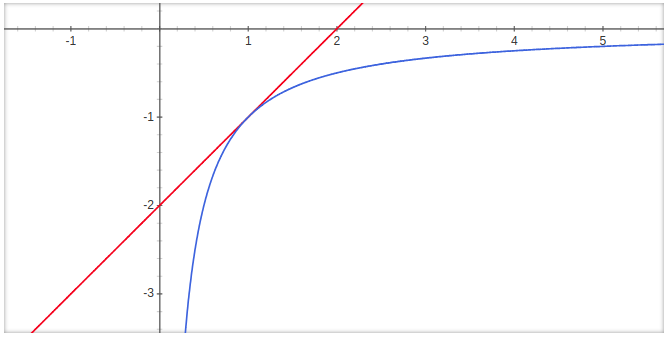
\includegraphics[width=0.49\textwidth]{derivata_00.png}\hfill%
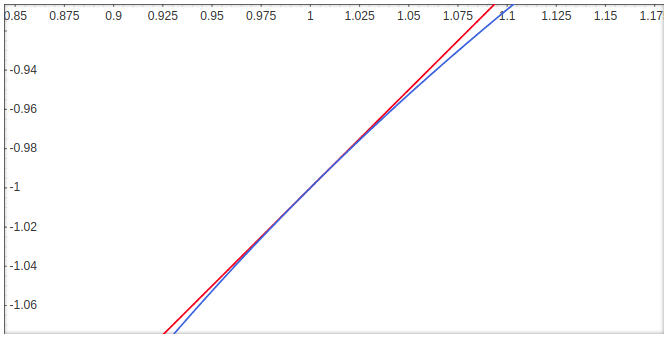
\includegraphics[width=0.49\textwidth]{derivata_01.png}
\label{fig:derivata}
\caption{Il grafico del potenziale gravitazionale terrestre.
Sull'asse delle $x$ la distanza dal centro della terra in raggi terrestri.
Sull'asse delle $y$ il potenziale gravitazionale con unità $C=GM/R$.
La pendenza della retta tangente al grafico della curva per $x=R$ è $g=GM/R^2$.
Nella figura di destra un ingrandimento in un intorno del raggio terrestre:
si nota come il grafico del potenziale risulta quasi indistinguibile dal
grafico della retta tangente.}
\end{figure}

Quello che abbiamo fatto è un procedimento di \myemph{linearizzazione}. Il campo gravitazionale è descritto da una funzione non lineare: $-GM/r$.
Ma quando ci restringiamo a un piccolo intervallo di valori di $r$ (i valori di $r$ vicini ad $R$, il raggio della terra) tale funzione risulta quasi indistinguibile, a meno di una costante, dalla funzione lineare $gh$ se $r=R+h$.
Le funzioni lineari sono molto più semplici da trattare ed è quindi conveniente, se rimaniamo sulla superficie terrestre, utilizzare quest'ultima formula per il potenziale gravitazionale.
Il grafico della funzione lineare che meglio approssima il grafico di una funzione si chiama \myemph{retta tangente}. Il suo coefficiente angolare, $g$ nel nostro esempio, si chiama \myemph{derivata}.

Una volta introdotte le derivate vedremo che quello che abbiamo
determinato è la formula:
\[
U(R+h) = U(R) + U'(R) h + \omega(h).
\]

\begin{definition}[derivata]
\mymark{***}
Sia $A\subset \RR$, $f\colon A \to \RR$, $x_0$ un punto di accumulazione di $A$.
Diremo che la funzione $f$ è \emph{derivabile} nel punto $x_0$ se esiste
ed è finito il limite:
\[
  \lim_{h\to 0} \frac{f(x_0+h) - f(x_0)}{h}.
\]
In tal caso denoteremo con $f'(x_0)$ il valore di tale limite che chiameremo
\myemph{derivata} della funzione $f$ nel punto $x_0$.

Se $B$ è l'insieme dei punti di accumulazione di $A$ in cui $f$ risulta essere derivabile, risulta quindi definita la funzione derivata $f'\colon B \to \RR$.

Una funzione $f$ si dice essere derivabile se è derivabile in ogni punto del suo dominio.
Se $C\subset A$ la funzione $f$ si dice essere \emph{derivabile su $C$} se è derivabile in ogni punto dell'insieme $C$ (cioè se $C\subset B$).

Notazioni alternative per denotare la derivata di una funzione:
\[
  f' = Df = \frac{d}{dx} f = \frac{df}{dx}.
\]
\end{definition}

Il rapporto
\[
\frac{f(x_0+h) - f(x_0)}{h}
\]
si chiama \myemph{rapporto incrementale}. In effetti cambiando variabile e ponendo $x=x_0+h$ si può scrivere
\[
\frac{f(x_0+h) - f(x_0)}{h}
= \frac{f(x) - f(x_0)}{x-x_0}
= \frac{\Delta f}{\Delta x}
\]
che risulta essere il rapporto dell'incremento della funzione $f$ (a volte denotato con $\Delta f$) rispetto all'incremento corrispondente della variabile $x$ (a volte denotato con $\Delta x$).
Cambiando variabile nel limite, per $h\to 0$ si avrà $x\to x_0$
e quindi
\[
 f'(x_0) = \lim_{x\to x_0} \frac{f(x)-f(x_0)}{x-x_0}.
\]

\begin{example}
\mymark{**}
Si consideri la funzione $f(x) = 1/x$ definita sull'insieme $A = \RR \setminus \ENCLOSE{0}$. Si ha allora per ogni $x\neq 0$:
\[
  f'(x) = \lim_{h\to 0} \frac{\frac{1}{x+h} - \frac{1}{x}}{h}
        = \lim_{h\to 0} \frac{x - (x+h)}{h(x+h)x}
        = \lim_{h\to 0} \frac{-1}{(x+h)x} = -\frac{1}{x^2}.
\]
Risulta quindi che la funzione $1/x$ sia derivabile e la sua derivata è la funzione $-1/x^2$.
\end{example}

\begin{theorem}[continuità delle funzioni derivabili]
\mymark{***}
Se $f$ è derivabile nel punto $x$ allora $f$ è anche continua nel punto $x$.
\end{theorem}
%
\begin{proof}
\mymark{***}
Si ha
\[
  \lim_{h\to 0} f(x+h) - f(x) = \lim_{h\to 0} \frac{f(x+h) - f(x)}{h} \cdot h
  = f'(x) \cdot 0 = 0.
\]
Dunque $f(x+h)\to f(x)$ per $h\to 0$ e quindi $f$ è continua nel punto $x$.
\end{proof}

\begin{example}[funzione continua ma non derivabile]
\mymark{***}
La funzione $f(x) = \abs{x}$ è un esempio di funzione continua ma non
derivabile. E' infatti facile verificare che nel punto $x_0=0$ il
limite destro del rapporto incrementale è $1$ mentre il limite
sinistro è $-1$.

Un altro esempio è la funzione $f(x) = \sqrt{x}$ che è continua ma non
è derivabile nel punto $x_0=0$ perché il limite del rapporto incrementale esiste ma è $+\infty$.
\end{example}



\begin{theorem}[derivata della funzione composta]
\mymark{**}
Sia $f$ una funzione derivabile nel punto $x_0$
e sia $g$ una funzione derivabile nel punto $f(x_0)$.
Allora la funzione composta $g\circ f$ è derivabile
nel punto $x_0$ e si ha:
\[
  (g\circ f)'(x_0) = g'(f(x_0))\cdot f'(x_0).
\]
\end{theorem}
%
\begin{proof}
\mymark{**}
Consideriamo la funzione
\[
  G(y) =
  \begin{cases}
   \frac{g(y) - g(f(x_0))}{y-f(x_0)} & \text{se $y \neq f(x_0)$},\\
   g'(f(x_0)) & \text{se $y=f(x_0)$}.
  \end{cases}
\]
Si avrà allora
\begin{equation}\label{eq:47439}
 \frac{g(f(x_0+h))-g(f(x_0))}{h}
 = G(f(x_0+h)) \cdot \frac{f(x_0+h)-f(x_0)}{h}
\end{equation}
infatti se $f(x_0+h)\neq f(x_0)$ abbiamo moltiplicato e diviso
per $f(x_0+h) - f(x_0)$ se invece $f(x_0+h)=f(x_0)$ allora anche $g(f(x_0+h))=g(f(x_0))$ e l'uguaglianza è ancora valida perché sia il lato sinistro che il lato destro si annullano (e il valore assegnato a $G$ risulta in tal caso irrilevante).

Chiaramente quando $h\to 0$ il secondo fattore sul lato destro
dell'uguaglianza \eqref{eq:47439}
tende, per definizione, a $f'(x_0)$.
Per quanto riguarda il primo fattore
osserviamo che $G(y)$, per come è stata definita, risulta essere una funzione continua nel punto $y=f(x_0)$ in quanto
\[
\frac{g(y) - g(f(x_0))}{y-f(x_0)} \to g'(f(x_0))
\]
per $y\to f(x_0)$.
Ma anche la funzione $f$ è continua nel punto $x_0$ (in quanto derivabile).
Dunque la funzione composta $G(f(x_0+h))$ è continua nel punto $h=0$.
Risulta quindi che $G(f(x_0+h)) \to G(f(x_0)) = g'(f(x_0))$ per $h\to 0$.
Dunque il lato destro di \eqref{eq:47439} ha limite $g'(f(x_0)) \cdot f'(x_0)$ per $h\to 0$, come volevamo dimostrare.
\end{proof}

\begin{theorem}[derivata della funzione inversa]
\mymark{**}
Sia $f$ una funzione invertibile derivabile in un punto $x_0$ e
supponiamo che la funzione inversa $f^{-1}$ sia continua in $f(x_0)$.
Se $f'(x_0)\neq 0$ allora $f^{-1}$ è derivabile in $f(x_0)$ e vale:
\[
  (f^{-1})'(f(x_0)) = \frac{1}{f'(x_0)}.
\]
Chiamato $y_0 = f(x_0)$ la formula può essere anche scritta nella forma:
\[
  (f^{-1})'(y_0) = \frac{1}{f'(f^{-1}(y_0))}.
\]
Se invece $f'(x_0)=0$ la funzione $f^{-1}$ non è derivabile in $f(x_0)$.
\end{theorem}
%
Osserviamo che se $f$ è definita in un intervallo e se è invertibile e
continua in tutto l'intervallo allora certamente l'inversa è continua
(Esercizio~\ref{ex:inversa_monotona}).
%
\begin{proof}
\mymark{**}
Posto $y_0 = f(x_0)$ consideriamo il rapporto incrementale di $f^{-1}$ nel punto $y_0$:
\[
  \frac{f^{-1}(y) - f^{-1}(y_0)}{y-y_0}.
\]
Per $y\to y_0$ possiamo fare il cambio di variabile
$x=f^{-1}(y)$ in quanto avendo assunto che $f^{-1}$ sia continua in $f(x_0)$ sappiamo che se $y\to y_0$ allora $x = f^{-1}(y)\to f^{-1}(y_0) = x_0$.
Si ha allora per $y\to y_0$ che $x\to x_0$ e,
se $f'(x_0)\neq 0$:
\[
  \frac{f^{-1}(y) - f^{-1}(y_0)}{y-y_0}
  = \frac{x-x_0}{f(x)-f(x_0)}
  = \frac{1}{\frac{f(x)-f(x_0)}{x-x_0}} \to \frac{1}{f'(x_0)}.
\]

Se invece $f'(x_0)=0$ il rapporto incrementale della funzione inversa
ha limite infinito e quindi la funzione inversa non è derivabile in $f(x_0)$.
\end{proof}


\begin{theorem}[operazioni con le derivate]
\mymark{***}
Siano $f$ e $g$ due funzioni derivabili in uno stesso punto $x_0$.
Allora le funzioni $f+g$, $f-g$, $f\cdot g$ e, se $g(x_0)\neq 0$ anche $f/g$ sono funzioni derivabili in $x_0$. Nei punti in cui entrambe le funzioni sono derivabili si ha
\begin{gather*}
  (f+g)' = f' + g', \qquad
  (f-g)' = f' - g', \\
  (f\cdot g)' = f' \cdot g + f g', \qquad
  \enclose{\frac{f}{g}}' = \frac{f'g - fg'}{g^2}.
\end{gather*}
\end{theorem}
%
\begin{proof}
\mymark{***}
Per quanto riguarda la derivata della somma (o della differenza) è sufficiente osservare che il rapporto incrementale della somma (o della differenza) è la somma (o la differenza) dei rapporti incrementali e che il limite della somma (o della differenza) è uguale alla somma (o la differenza) dei limiti.

Calcoliamo la derivata del prodotto $f\cdot g$ nel punto $x_0$. Si ha
\begin{align*}
  \frac{f(x)g(x) - f(x_0)g(x_0)}{x-x_0}
  &= \frac{f(x)(g(x) - g(x_0)) + (f(x)-f(x_0))g(x_0)}{x-x_0}\\
  &= f(x) \frac{g(x)-g(x_0)}{x-x_0} + \frac{f(x)-f(x_0)}{x-x_0} g(x_0).
\end{align*}
Passando al limite per $x\to x_0$ ci ricordiamo che $f(x)\to f(x_0)$ in quanto $f$ è continua in $x_0$ (essendo per ipotesi derivabile). I rapporti incrementali tendono alle derivate e si ottiene quindi il risultato voluto $f(x_0) g'(x_0) + f'(x_0) g(x_0)$.

Per quanto riguarda la derivata del rapporto osserviamo che
posto $h(y)=1/y$ si ha
\[
  \frac{f(x)}{g(x)} = f(x) \cdot h(g(x)).
\]
Dall'esercizio già svolto sappiamo che $h'(y) = -1/y^2$ e dunque
possiamo utilizzare le formule per la derivata del prodotto e la derivata della funzione composta per ottenere:
\begin{align*}
  \enclose{\frac{f}{g}}'(x_0)
  &= \enclose{f \cdot (g\circ h)}'(x_0) \\
  &= f'(x_0) \cdot h(g(x_0)) + f(x_0) \cdot h'(g(x_0))\cdot g'(x_0)\\
  &= \frac{f'(x_0)}{g(x_0)} + f(x_0) \cdot \frac{-1}{g^2(x_0)} g'(x_0)\\
  &= \frac{f'(x_0)g(x_0) - f(x_0)g'(x_0)}{g^2(x_0)}.
\end{align*}
\end{proof}

\begin{theorem}[derivate delle funzioni elementari]
\index{derivata!delle funzioni elementari}
\mymark{**}
Per $m,q,\alpha \in \RR$, $\alpha \neq 0$, $n\in \NN$, $n\neq 0$
si ha
\begin{gather*}
D (mx + q) = m, \qquad
D \abs{x} = \frac{x}{\abs{x}}, \qquad
D x^n = n x^{n-1}, \\
D x^\alpha = \alpha x^{\alpha -1}, \qquad
D \sqrt[n]{x} = \frac{1}{n\sqrt[n]{x^{n-1}}}, \qquad
D \sqrt{x} = \frac{1}{2\sqrt{x}}
\\
D e^x = e^x, \qquad
D \ln x = 1/x \\
D \sin x = \cos x, \qquad D \cos x = -\sin x\\
D \arcsin x =  \frac{1}{\sqrt{1-x^2}}, \qquad
D \arccos x = -\frac{1}{\sqrt{1-x^2}},\\
D \tg x = 1+ \tg^2 x = \frac{1}{\cos^2 x},
\qquad D \arctg x = \frac{1}{1+x^2},\\
D \sinh x = \cosh x,
\qquad D \cosh x = \sinh x,\\
D \settsinh x = \frac{1}{\sqrt{x^2+1}}, \qquad
D \settcosh x = \frac{1}{\sqrt{x^2-1}}.
\end{gather*}
dove le uguaglianze sono valide (e quindi le funzioni sul lato sinistro sono derivabili) nei punti in cui il lato destro è ben definito.
La funzione $\sqrt[n]{x}$
non è derivabile in $x=0$.
Le funzioni $\arcsin x$ e $\arccos x$ non sono derivabili nei punti $-1$ e $1$.
La funzione $\abs{x}$ non è derivabile in $0$.
La funzione $\settcosh x$ non è derivabile in $1$.
Le funzioni lineari, potenze con base positiva, potenze con esponente intero,
esponenziale, logaritmo, seno, coseno, tangente, arcotangente sono invece derivabili
in tutti i punti in cui sono definite.
\end{theorem}

\begin{proof}
\mymark{**}
Per quanto riguarda le funzioni lineari si ha:
\begin{align*}
(mx+q)' &= \lim_{h\to 0}\frac{m(x+h)+q - (mx+q)}{h} = \lim_{h\to 0} m = m.
\end{align*}
Ricordando che la derivata è un limite e che il limite in un punto dipende solo dai valori della funzione in un intorno del punto, possiamo affermare che la derivata del valore assoluto $\abs{x}$ coincide con la derivata di $x$ cioè $1$ sugli $x>0$ e coincide con la derivata di $-x$ sugli $x<0$. Dunque $D \abs{x} = x / \abs{x}$ se $x\neq 0$. Se $x=0$ i limiti destro e sinistro del rapporto incrementale di $\abs{x}$ tendono rispettivamente a $1$ e $-1$ e quindi la derivata non esiste.

Dimostriamo che $Dx^n = n D x^{n-1}$ per $n\in \NN$, $n>0$, per induzione su $n$. Per $n=1$ abbiamo $x^n=x^1$ è lineare e quindi dalla formula precedente $Dx^1 = 1 = 1 \cdot x^0$. Supponendo di sapere che $D x^n = n x^{n-1}$ si ha, applicando la regola di derivazione del prodotto:
\[
  D x^{n+1} = D x\cdot x^n = 1 \cdot x^n + x \cdot n x^{n-1}
   = x^n + n x^n = (n+1) x^n
\]
dimostrando dunque il passo induttivo.
Ricordando la formula di derivazione del rapporto
possiamo trovare la formula per le potenze con esponente intero negativo:
\[
  D x^{-n} = D \frac{1}{x^n} = \frac{-n x^{n-1}}{x^{2n}}
   = -n x^{n-1-2n} = -n x^{-n-1}.
\]

La derivata della radice $n$-esima si trova con la formula di derivazione della funzione inversa $x^n$, che può essere applicata se $x\neq 0$:
\[
  D \sqrt[n]{x} = \frac{1}{n(\sqrt[n]{x})^{n-1}}
    = \frac{1}{n\sqrt[n]{x^{n-1}}}.
\]
Osserviamo che se $n$ è dispari la formula è valida anche per $x<0$.
La derivata della radice quadrata si ottiene ponendo $n=2$.

Per quanto riguarda la derivata dell'esponenziale
ci riconduciamo ad un limite notevole:
\[
  D e^x = \lim_{h\to 0} \frac{e^{x+h}-e^x}{h}
  = \lim_{h\to 0}\frac{e^x e^h - e^x}{h}
  = \lim_{h\to 0}e^x \frac{e^h - 1}{h}
  = e^x.
\]
La derivata del logaritmo si ottiene come derivata della funzione inversa dell'esponenziale:
\[
  D \ln x = \frac{1}{e^{\ln x}} = \frac{1}{x}.
\]
Possiamo quindi calcolare la derivata delle potenze con base positiva e esponente reale qualunque:
\[
D x^\alpha
= D e^{\alpha \ln x}
= e^{\alpha \ln x} D(\alpha \ln x)
= x^\alpha \alpha \frac{1}{x}
= \alpha x^{\alpha -1}.
\]

Per quanto riguarda le funzioni trigonometriche $\sin$ e $\cos$ ci ricordiamo dei limiti notevoli:
\[
  \lim_{h\to 0}\frac{\sin h}{h} = 1,\qquad
  \lim_{h\to 0}\frac{1-\cos h}{h}
  =\lim_{h\to 0}h \cdot \frac{1-\cos h}{h^2} = 0 \cdot \frac{1}{2} = 0.
\]
Applicando le formule di addizione si ha
\begin{align*}
  D \sin x
  &= \lim_{h\to 0}\frac{\sin(x+h)-\sin(x)}{h} \\
  &= \lim_{h\to 0}\frac{\sin(x)\cos(h) + \cos(x)\sin(h) - \sin(x)}{h} \\
  &= \lim_{h\to 0}\sin(x) \frac{\cos h-1}{h} + \cos(x) \frac{\sin h}{h} = \cos(x).
\end{align*}
e similmente
\begin{align*}
  D \cos x
  &= \lim_{h\to 0}\frac{\cos(x+h)-\cos(x)}{h} \\
  &= \lim_{h\to 0}\frac{\cos(x)\cos(h) - \sin(x)\sin(h) - \cos(x)}{h} \\
  &= \lim_{h\to 0}\cos(x) \frac{\cos h-1}{h} - \sin(x) \frac{\sin h}{h} = -\sin(x)
\end{align*}

La funzioni $\arcsin$ è definita come l'inversa della restrizione della funzione $\sin$ all'intervallo $[-\pi/2, \pi/2]$.
Nell'intervallo aperto $(-\pi/2,$ $\pi/2)$ la funzione $\sin$ ha derivata positiva e dunque risulta che la funzione inversa (che sappiamo essere continua) è derivabile in $(-1,1)$ e la sua derivata è
\[
D\arcsin x
= \frac{1}{\cos(\arcsin x)}
= \frac{1}{\sqrt{1-\sin^2 \arcsin x}}
= \frac{1}{\sqrt{1-x^2}}.
\]
Si ha infatti $\cos y = \sqrt{1-\sin^2 y}$ se $y\in [-\pi/2, \pi/2]$.

Analogamente la funzione $\arccos$ è definita come l'inversa della restrizione di $\cos$ all'intervallo $[0,\pi]$ e si ha quindi,
per $x\in (-1,1)$
\[
D \arccos x
 = \frac{1}{-\sin(\arccos x)}
 = \frac{1}{-\sqrt{1-\cos^2 \arccos x}}
 = -\frac{1}{\sqrt{1-x^2}}.
\]
Si ha infatti $\sin y = \sqrt{1-\cos^2 y}$ se $y\in[0,\pi]$.

Nei punti $x=1$ e $x=-1$ le funzioni $\arcsin$ e $\arccos$ non sono invece derivabili.

Per la funzione tangente possiamo utilizzare la formula di derivazione del rapporto:
\begin{align*}
  D \tg x &= D \frac{\sin x }{\cos x}
   = \frac{\cos x \cdot \cos x - \sin x \cdot (-\sin x)}{\cos^2 x} \\
   &= \frac{\cos^2 x + \sin^2 x}{\cos^2 x}
   = 1 + \tg^2 x = \frac{1}{\cos^2 x}.
\end{align*}
Usando la formula della derivata della funzione inversa si ha
\[
  D \arctg x = \frac{1}{1+\tg^2(\arctg x)}
  = \frac{1}{1+x^2}.
\]

Per quanto riguarda le funzioni iperboliche le derivate di $\sinh$
e $\cosh$ si riconducono immediatamente alla derivata dell'esponenziale,
utilizzando
la definizione~\eqref{eq:sinh_cosh}. Le derivate delle funzioni
inverse $\settsinh$ e $\settcosh$ si ottengono dalla formula per la derivata
della funzione inversa e utilizzando
le relazioni $\cosh x = \sqrt{\sinh^2 x+1}$ e, per $x > 0$,
$\sinh x = \sqrt{\cosh^2 x -1}$:
\begin{align*}
  D \settsinh x &= \frac{1}{\cosh(\settsinh x)}
  = \frac{1}{\sqrt{\sinh^2 (\settsinh x) + 1}} = \frac{1}{\sqrt{x^2+1}}\\
  D \settcosh x &= \frac{1}{\sinh(\settcosh x)}
  = \frac{1}{\sqrt{\cosh^2(\settcosh x)-1}}
  = \frac{1}{\sqrt{x^2-1}}
\end{align*}
\end{proof}

\section{nomenclatura}

In questa sezione introdurremo una terminologia che è largamente utilizzata 
nello studio di funzione.
Cercheremo di dare delle definizioni anche per alcuni termini su cui potrebbe 
non esserci un consenso univoco.
Ricordiamoci di non usare queste definizioni in modo troppo formale:
sarà sempre meglio
verificare che il nostro interlocutore ci comprenda
perché spesso alcuni termini potrebbero essere utilizzati in maniera
impropria o con significati leggermente diversi.

Nel dubbio potremo sempre evitare di utilizzare questa terminologia 
riconducendoci ai concetti sottostanti.

\begin{definition}[punti notevoli]
Sia $f\colon A \subset \RR \to \RR$ una funzione. Se $f$ è derivabile in un
punto $x_0\in A$ e $f'(x_0) = 0$ diremo che $x_0$ è un \myemph{punto!critico}
o
\emph{punto stazionario}
\index{punto!stazionario}
di $f$.

Se $x_0\in A$ ed esiste un intorno $U$ di $x_0$ per cui $x_0$ risulta
essere un punto di minimo (rispettivamente di massimo) per $f$ ristretta ad $U$
diremo che $x_0$ è un punto di \myemph{minimo relativo} o \emph{minimo locale}
(rispettivamente \emph{massimo relativo} o \emph{massimo locale}).
Per contrapposizione i punti di massimo e minimo su tutto il dominio $A$
vengono anche
chiamati massimo/minimo \emph{assoluto} di $f$.

Diremo che $x_0\in A$ è un \myemph{punto!di flesso} per $f$ se
$f$ è derivabile in un intorno di $x_0$ e $x_0$ è un punto di massimo
o minimo relativo per $f'$. Nel punto $x_0$ la retta tangente
ha equazione $y=r(x) = f'(x_0) (x-x_0) + f(x_0)$. Se $x_0$ è
minimo per $f'$ risulta che $f(x)-r(x)$ è crescente
quindi $f(x)\ge r(x)$ per $x\ge x_0$ e $f(x)\le r(x)$ per $x\le x_0$
(il grafico della funzione attraversa la retta tangente da sotto a sopra)
mentre se $x_0$ è massimo per $f'$ risulta che $f(x)\le r(x)$ per $x\ge x_0$
e $f(x) \ge r(x)$ per $x\le x_0$ (il grafico della funzione attraversa
la tangente da sopra a sotto).
Se la funzione $f$ non è derivabile in $x_0$ ma il limite del rapporto
incrementale esiste ed è infinito, diremo che $x_0$ è un
\myemph{flesso verticale}. In tale punto la retta tangente è verticale
e il grafico della funzione attraversa tale retta.

Sia $x_0\in A$ un punto in cui la funzione $f$ è continua ed esistono
i limiti destro e sinistro del rapporto incrementale
(che si chiamano \emph{derivata destra} e \emph{derivata sinistra})
\[
  m^{\pm} = \lim_{h\to 0^\pm}\frac{f(x+h) - f(x)}{h}.
\]
Se $m^+ \neq m^-$ chiaramente $f$ non è derivabile in $x_0$.
Se entrambi $m^+$ ed $m^-$ sono finiti diremo che $x_0$ è un
\myemph{punto!angoloso} in quanto le due semirette tangenti
in $x_0$ (da destra e da sinistra) formano un angolo non piatto.
Se $m^+=-m^-=+\infty$ oppure se $m^+=-m^-=-\infty$
diremo che il punto $x_0$ è un \myemph{punto!di cuspide} (c'è una
semiretta tangente verticale).
\end{definition}

\begin{definition}[asintoti]
Diremo che la retta $y=mx+q$ è un asintoto per il grafico di $f$ 
per $x\to +\infty$ se risulta
\[
  \lim_{x\to +\infty} f(x) - (mx+q) = 0.
\]
Se $m=0$ diremo che il grafico di $f$ ha un \emph{asintoto orizzontale} $y=q$
\mymargin{asintoto orizzontale/obliquo}%
\index{asintoto!orizzontale}%
\index{asintoto!obliquo}%
altrimenti diremo che $y=mx+q$ è un \emph{asintoto obliquo}.
Stessa cosa si può dire per $x\to -\infty$.

Se $x_0\in \RR$ e si ha 
\[
  \lim_{x\to x_0} \abs{f(x)} = +\infty
\]
diremo che la retta $x=x_0$ è un \myemph{asintoto!verticale} per il 
grafico della funzione $f$.
\end{definition}

\begin{definition}[punti di discontinuità]
Se per $x_0\in \RR$ si ha 
\[
  \lim_{x\to x_0^-} f(x) = \ell_1, 
  \qquad 
  \lim_{x\to x_0^+} f(x) = \ell_2
\]
e se $\ell_1\neq \ell_2$ diremo che nel punto $x_0$ 
la funzione $f$ ha una \myemph{discontinuità a salto}.
Se $\ell_1=\ell_2$ e se $f$ non è definita nel punto $x_0$ 
oppure se $f(x_0)\neq \ell_1$ diremo che 
nel punto $x_0$ la funzione $f$ 
ha una \myemph{discontinuità eliminabile}.
\end{definition}

Si osservi che, nonostante la terminologia utilizzata,
una funzione continua può avere una discontinuità 
a salto (ad esempio: $f(x)=\frac{x}{\abs{x}}$) 
e può anche avere una discontinuità eliminabile
(ad esempio: $f(x) = \frac{x}{x}$).

\section{criteri di monotonia}

\begin{theorem}[Fermat]
\mymark{***}
Sia $f\colon (a,b)\to \RR$ una funzione derivabile.
Se $x_0\in (a,b)$ è un punto di massimo o minimo per $f$ allora
$f'(x_0)=0$.
\end{theorem}
%
\begin{proof}
\mymark{***}
Senza perdere di generalità possiamo suppore che $x_0$ sia un punto di massimo per $f$.
Sappiamo che
\[
  f'(x_0) = \lim_{x\to x_0}\frac{f(x)-f(x_0)}{x-x_0}.
\]
Visto che $x_0$ è un punto dell'intervallo aperto $(a,b)$ la funzione $f$ è definita in un intorno destro di $x_0$ e quindi possiamo restingere il limite ai valori $x>x_0$ ottenendo:
\[
  f'(x_0) = \lim_{x\to x_0^+}\frac{f(x) - f(x_0)}{x-x_0}.
\]
Visto che $x_0$ è un punto di massimo per $f$ sappiamo che $f(x)-f(x_0)\le 0$. Essendo $x-x_0>0$ l'intero rapporto incrementale risulta essere non positivo.
Dunque, per il teorema della permanenza del segno,
possiamo concludere che $f'(x_0)\le 0$.

Ma possiamo anche restringere la funzione ad un intorno sinistro di $x_0$ e osservare che
\[
  f'(x_0) = \lim_{x\to x_0^-}\frac{f(x)-f(x_0)}{x-x_0}.
\]
Ma ora il numeratore è, come prima, non positivo mentre il denominatore $x-x_0$ è negativo. Dunque il rapporto incrementale stavolta è non negativo e quindi, per la permanenza del segno, $f'(x_0) \ge 0$.

Abbiamo scoperto quindi che $f'(x_0)\le 0$ e $f'(x_0)\ge 0$
da cui deduciamo $f'(x_0)=0$.
\end{proof}

Il teorema di Fermat si può
enunciare dicendo che ogni punto di massimo o minimo relativo interno
al dominio di una funzione in cui la funzione è derivabile
è necessariamente un punto critico.
In particolare per determinare massimi e minimi assoluti e relativi
di una funzione sarà sufficiente esaminare i punti di frontiera,
i punti di non derivabilità e i punti critici.


\begin{theorem}[Rolle]
\mymark{***}
\index{teorema!di Rolle}
\mymargin{Rolle}
Sia $f\colon [a,b]\to \RR$ una funzione continua su tutto $[a,b]$ e derivabile su $(a,b)$. Se $f(a) = f(b)$ allora esiste $x_0 \in (a,b)$ tale che $f'(x_0)=0$.
\end{theorem}
%
\begin{proof}
\mymark{***}
Essendo $f$ una funzione continua
possiamo applicare il teorema di Weiestrass per dedurre che $f$ ha massimo e 
minimo sull'intervallo chiuso e limitato $[a,b]$. 
Se il punto di massimo o il punto di minimo sta nell'intervallo aperto 
$(a,b)$ possiamo applicare il teorema di Fermat per ottenere che la derivata 
di $f$ si annulla in tale punto.

In caso contrario sia il punto di massimo che il punto di minimo sono estremi 
dell'intervallo, cioè sono uguali ad $a$ o a $b$. Ma visto che $f(a)=f(b)$ 
i valori massimo e minimo coincidono e quindi la funzione è costante. 
Ma in tal caso $f'(x)=0$ per ogni $x\in [a,b]$.
\end{proof}

\begin{theorem}[Lagrange]\label{th:lagrange}%
\mymark{***}%
\index{teorema!di Lagrange}%
\mymargin{Lagrange}%
Sia $f\colon [a,b]\to \RR$ una funzione continua su $[a,b]$ e derivabile su $(a,b)$. Allora esiste un punto $x_0\in (a,b)$ tale che
\[
  f'(x_0) = \frac{f(b) - f(a)}{b-a}
\]
\end{theorem}
%
\begin{proof}
\mymark{***}
Consideriamo la funzione ausiliaria:
\[
  g(x) = f(x) - \frac{f(b)-f(a)}{b-a} x.
\]
Per verifica diretta si osserva che
\[
  g(b) = g(a) = \frac{b f(a) - a f(b)}{b-a}.
\]
La funzione $g$ soddisfa quindi le ipotesi del teorema di Rolle e dunque esisterà $x_0\in (a,b)$ tale che $g'(x_0)=0$.
Ma si osserva che
\[
  g'(x) = f'(x) - \frac{f(b)-f(a)}{b-a}
\]
e dunque se $g'(x_0)=0$ si ottiene il risultato desiderato.
\end{proof}

\begin{theorem}[criteri di monotonia]%
\label{th:criteri_monotonia}
\mymark{***}%
\mynote{criteri di monotonia}%
\index{criterio!di monotonia}%
Sia $f\colon I \to \RR$ una funzione definita su un intervallo $I\subset \RR$. Sia $J= (\inf I, \sup I)$ l'intervallo aperto con gli stessi estremi di $I$.
Supponiamo che $f$ sia continua su $I$ e derivabile su $J$. Allora valgono i seguenti criteri:
\begin{enumerate}
\item
$(\forall x \in J\colon f'(x)\ge 0)$
$\iff$
$f$ è crescente (su tutto $I$);
\item
$(\forall x \in J\colon f'(x)\le 0)$
$\iff$
$f$ è decrescente (su tutto $I$);
\item
$(\forall x \in J\colon f'(x)=0)$
$\iff$
$f$ è costante (su tutto $I$);
\item
$(\forall x \in J\colon f'(x)>0)$
$\implies$
$f$ è strettamente crescente (su tutto $I$);
\item
$(\forall x \in J\colon f'(x)<0)$
$\implies$
$f$ è strettamente decrescente (su tutto $I$).
\end{enumerate}
\end{theorem}
%
\begin{proof}
\mymark{***}
Dimostriamo innanzitutto le implicazioni da sinistra verso destra.

Per la prima, se $f$ non fosse crescente ci dovrebbero essere due punti $a, b \in I$ tali che $a < b$ ma $f(a) > f(b)$.
Dunque si avrebbe
\[
  \frac{f(b) - f(a)}{b - a} < 0.
\]
Applicando il teorema di Lagrange all'intervallo $[a,b]$ si troverebbe un punto $x\in (a,b)$ tale che $f'(x) < 0$. Chiaramente $(a,b)\subset J$ e quindi questo contraddice l'ipotesi $f'(x) \ge 0$.

La seconda implicazione (per le funzioni decrescenti) si dimostra in maniera analoga cambiando verso alle disuguaglianze.

Anche la terza implicazione si dimostra tramite il teorema di Lagrange in modo analogo alle precedenti. Oppure basta osservare che se $f'(x)=0$ allora valgono contemporaneamente $f'(x)\ge 0$ e $f'(x)\le 0$ quindi mettendo insieme le prime due implicazioni si ottiene che $f$ è contemporaneamente crescente e decrescente dunque è costante.

Per la quarta implicazione si procede come per la prima. Per assurdo si  avrebbero $a<b$ con $f(b) \le f(a)$. Ma allora
\[
  \frac{f(b) - f(a)}{b-a} \le 0
\]
e applicando il teorema di Lagrange si troverebbe un punto $x\in (a,b)$ con $f'(x) \le 0$, contro l'ipotesi $f'(x) > 0$.

La quinta implicazione si dimostra in maniera analoga cambiando verso alle disuguaglianze.

Vediamo ora le implicazioni da destra verso sinistra.
Per la prima, supponiamo che $f$ sia crescente e prendiamo $x\in J$. Allora è chiaro che per ogni $h>0$ si avrà $f(x+h) \ge f(x)$ e dunque
\[
  \frac{f(x+h)- f(x)}{h} \ge 0.
\]
Facendo il limite per $h \to 0^+$ si ottiene $f'(x)$ e, per la permanenza del segno, dovra essere $f'(x) \ge 0$.

In maniera analoga (invertendo le disuguaglianze) si dimostra la seconda implicazione.

La terza discende dalle prime due oppure, più semplicemente, dalle regole di derivazione, in quanto la derivata di una costante è zero.
\end{proof}

\begin{example}
La funzione $f(x) = 1/x$ è definita su $\RR \setminus \ENCLOSE{0}$, è derivabile
e la derivata $f'(x) = -1/x^2$ è ovunque negativa. La funzione $f$ è quindi strettamente
decrescente separatamente sui due intervalli $(0,+\infty)$ e $(-\infty,0)$ sui quali
possiamo applicare il criterio di monotonia. Ma non è
decrescente su tutto il suo dominio in quanto, ad esempio, $f(-1) = -1 < 1 = f(1)$.
Questo esempio mostra che nei criteri di monotonia l'ipotesi che il dominio sia un intervallo
è fondamentale.
\end{example}

\begin{exercise}
\index{problema!della lattina}%
\index{lattina!problema della}%
Determinare base e altezza di una lattina cilindrica di volume $33 cl$
che a parità di volume ha la minima superficie totale.
\end{exercise}
\begin{proof}[Svolgimento.]
Sia $V$ il volume, $S$ l'area della superficie totale, $h$ l'altezza e $r$
il raggio di base del cilindro.
Sappiamo che
\[
  V = \pi h r^2 \\
  S = 2\pi r h + 2 \pi r^2.
\]
Ricavando $h$ dalla prima equazione e sostituendo nella seconda otteniamo
\[
  S = 2 \pi r \frac{V}{\pi r^2} + 2 \pi r^2
    = \frac{2V}{r} + 2 \pi r^2.
\]
La funzione $S(r)$ è definita e continua su $(0,+\infty)$
e si ha $S(r)\to +\infty$ per $r\to 0^+$
e anche per $r\to +\infty$. Dunque $S$ ammette minimo per il teorema di Weierstrass
generalizzato.
Per trovare il minimo basterà calcolare la derivata
\[
 \frac{dS}{dr} = -\frac{2V}{r^2} + 4 \pi r = \frac{4\pi r^3 - 2V}{r^2}
\]
e trovare i punti critici
\[
  4\pi r^3 = 2V
\]
da cui
\begin{align*}
 r = \sqrt[3]{\frac{V}{2\pi}} \approx 3.74 cm\\
 h = \frac{V}{\pi r^2} \approx 7.49 cm.
\end{align*}
\end{proof}

\begin{exercise}
Risolvere l'equazione
\begin{equation} \label{eq:4734521}
  e^x = x^3.
\end{equation}
\end{exercise}
%
\begin{proof}[Svolgimento.]
Il lato sinistro dell'equazione è un numero positivo e quindi
certamente possiamo supporre che sia $x>0$ altrimenti il lato destro non sarebbe anch'esso positivo.
Possiamo quindi prendere il logaritmo di ambo i membri
e ottenere l'equazione
\[
  x = 3 \ln x
\]
che è equivalente all'equazione data.

Consideriamo allora la funzione
\[
 f(x) = x - 3 \ln x
\]
cosicché le soluzioni cercate risultano essere gli zeri di $f$.
Si ha
\[
  f'(x) = 1 - \frac{3}{x}
\]
e possiamo quindi affermare che%
\footnote{Il simbolo $\gtrless$ serve per indicare che questa
diseguazione e le seguenti possono essere scritte sia con il segno
$>$ che con il segno $<$ pur di prendere in tutte lo stesso segno.}
 $f'(x) \gtrless 0$
se e solo se
\[
  1 \gtrless \frac 3 x
\]
ovvero (ricordiamo che stiamo supponendo $x>0$)
\[
  x \gtrless 3.
\]
Cioè: se $x>3$ si ha $f'(x)>0$ e di conseguenza
(teorema~\ref{th:criteri_monotonia})
$f$ è strettamente crescente se ristretta all'intervallo
$[3,+\infty)$,
se invece $x<3$ si ha $f'(x)<0$ e di conseguenza
$f$ è strettamente decrescente se ristretta all'intervallo
$(0,3]$.
Per capire se la funzione $f$ si annulla in qualche punto
dobbiamo ora valutare $f$ negli estremi degli intervalli su cui risulta monotona. Si ha
\[
  \lim_{x\to 0^+} f(x) = +\infty, \qquad
  f(3) = 3 (1 - \ln 3) <0, \qquad
  \lim_{x\to +\infty} f(x) = +\infty.
\]
Osserviamo quindi che agli estremi degli intervalli
$(0,3]$ e $[3,+\infty)$ la funzione assume segni opposti e quindi, per il teorema degli zeri (teorema~\ref{th:zeri}), deve annullarsi almeno una volta in ognuno dei due intervalli. D'altra parte su ognuno dei due intervalli la funzione è strettamente monotona e quindi iniettiva, dunque non può annullarsi più di una volta. Deduciamo quindi che la funzione $f$ si annulla in esattamente due punti $x_1$, $x_2$ con
\[
  0 < x_1 < 3 < x_2.
\]

I punti $x_1$ e $x_2$ sono quindi univocamente determinati
e possono essere calcolati, con un errore piccolo a piacere,
utilizzando il metodo di bisezione, come abbiamo
visto nella dimostrazione del teorema degli zeri.
\end{proof}

\begin{comment} %% dimostrazione più lunga e complicata
\begin{proof}
Si consideri la funzione
\[
  f(x) = e^x - x^3.
\]
Dobbiamo trovare gli zeri di $f$ (cioè i punti $x$ tali che $f(x)=0$).
Si ha
\begin{align*}
  f'(x) &= e^x- 3x^2,\\
  f''(x) &= e^x - 6x,\\
  f'''(x) &= e^x - 6.
\end{align*}
Si ha $f'''(x) \gtreqqless 0$ se $x \gtreqqless \ln 6$.
Applicando i criteri di monotonia possiamo quindi dedurre che
$f''$ (la cui derivata è $f'''$) è strettamente decrescente sull'intervallo $(-\infty , \ln 6]$
e strettamente crescente sull'intervallo $[\ln 6, +\infty)$.
Di conseguenza $\ln 6$ è un punto di minimo per $f''$ su tutto $\RR$.
Possiamo rappresentare sinteticamente queste
proprietà in forma di tabella, come segue.
\begin{center}
\begin{tabular}{c|c c c}
  $x$ & & $\ln 6$ & \\ \hline
  $f'''(x)$ & $-$ & $0$ & $+$ \\
  $f''(x)$ & $\searrow$ & $\min$ & $\nearrow$
\end{tabular}
\end{center}
Cerchiamo di determinare il segno di $f''$ agli estremi degli intervalli su
cui $f''$ è monotona.
Per $x\to -\infty$ si ha $f''(x)\to +\infty$, per $x\to +\infty$ si ha $f''(x)\to +\infty$
e per $x=\ln 6$ si ha $f''(\ln 6)=6-6\ln 6 < 0$.
Dunque sui due intervalli $(-\infty,\ln 6]$ e $[\ln 6,+\infty]$ la funzione $f''$
è strettamente monotona e cambia segno. Per il teorema degli zeri tale funzione
si annulla in ognuno dei due intervalli e per la stretta monotonia si annulla
in un solo punto su ogni intervallo. Dunque esistono $x_1$ e $x_2$ tali che
$x_1 < \ln 6 < x_2$ e $f''(x_1) = f''(x_2) = 0$. Dalla monotonia di $f''$ possiamo
quindi dedurre i segni di $f''$ e quindi l'andamento di $f'$.
\begin{center}
\begin{tabular}{c|c c c c c}
$x$      &   & $x_1$ &   & $x_2$ &   \\ \hline
$f''(x)$ & $+$ &  $0$  & $-$ &  $0$    & $+$ \\
$f'(x)$  & $\nearrow$ & $\max$ & $\searrow$ & $\min$ & $\nearrow$
\end{tabular}
\end{center}
Nel precedente diagramma si intende che i punti $x_1$ e $x_2$
sono massimo e minimo \emph{relativo} in quanto $x_1$ è massimo
per $f'$ sull'intervallo $(-\infty,x_2]$ e $x_2$ è minimo di $f$
sull'intervallo $[x_1, +\infty)$.

Come prima vogliamo determinare il segno di $f'$ guardando il segno agli
estremi dei suoi intervalli di monotonia.
Per $x\to -\infty$ si ha $f'(x) \to -\infty$,
per $x\to +\infty$ si ha $f'(x)\to +\infty$.
Siamo anche in grado di determinare il segno di $f'(x_1)$ e $f'(x_2)$
sfruttando le proprietà algebriche di tali numeri.
Sappiamo infatti che $x_1$ e $x_2$ risolvono l'equazione $e^x = 6x$. Dunque
\[
  f'(x_1) = e^{x_1} - 3x_1^2 = 6x_1 - 3 x_1^2 = 3x_1 (2-x_1)
\]
e lo stesso vale per $f'(x_2)$.

Ora possiamo capire dove si trovano $x_1$ e $x_2$ rispetto ai valori $0$ e $2$
guardando semplicemente il segno di $f''(0) = 1 > 0$ e $f''(2) = e^2 - 12 < 0$.
Visto che $f''(2)<0$ guardando la tabella dei segni di $f''$
possiamo concludere che $x_1 < 2 < x_2$.
Analogamente visto che $f''(0)>0$ e $0<2<x_2$ possiamo dedurre
che $0 < x_1$. Dunque $0 < x_1 < 2 < x_2$ e
\[
  f'(x_1) = 3 x_1 (2-x_1) > 0,
  \qquad
  f'(x_2) = 3 x_2 (2-x_2) < 0.
\]
Conoscendo l'andamento di $f'$ possiamo costruire una tabella dei segni
di $f'$ dove inseriamo anche i limiti a $+\infty$ e $-\infty$.
\begin{center}
\begin{tabular}{c | c c c c c c c c c }
$x$ & $-\infty$ & & $x_1$ & & $x_2$ & & $+\infty$ \\ \hline
$f'(x)$ & $-$ & $\nearrow$ & $+$ & $\searrow$ & $-$ & $\nearrow$ & $+$\\
\end{tabular}
\end{center}
In base al teorema degli zeri e alla stretta monotonia possiamo quindi
affermare che $f'$ si annulla in esattamente tre punti $x_3$, $x_4$ e $x_5$
tali che $x_3 < x_1 < x_4 < x_2 < x_5$.
Con l'andamento di $f'$ possiamo quindi fare una tabella dei segni di $f'$.
\begin{center}
\begin{tabular}{c | c c c c c c c}
$x$ & & $x_3$ & & $x_4$ & & $x_5$ & \\ \hline
$f'(x)$ & $-$ & $0$ & $+$ & $0$ & $-$ & $0$ & $+$ \\
$f(x)$ & $\searrow$ & $\min$ & $\nearrow$ & $\max$ & $\searrow$ & $\min$ & $\nearrow$
\end{tabular}
\end{center}

Nuovamente vogliamo determinare il segno di $f$ negli estremi degli intervalli di monotonia:
$-\infty$, $x_3$, $x_4$, $x_5$, $+\infty$. In $-\infty$ e $+\infty$ è facile osservare che $f(x)$
tende a $+\infty$. Nei punti $x_3$, $x_4$ e $x_5$ possiamo sfruttare il fatto che tali punti,
essendo zeri di $f'$,
soddisfano l'equazione $e^x=3x^2$ dunque
\[
  f(x_3) = e^{x_3} - x_3^3 = 3x_3^2 - x_3^3 = x_3^2 (3 - x_3).
\]
Lo stesso vale per $f(x_4)$ e $f(x_5)$. Valutiamo $f'$ nei punti $0$ e $3$ per determinare
il segno dell'espressione precedente. Si ha $f'(0) = 1 > 0$ e $f'(3) = e^3 - 27 < 0$.
Guardando la tabella dei segni di $f'$ si può quindi affermare che $x_3 < 0 < x_1 < x_4 < 3 < x_5$.
Dunque
\begin{align*}
  f(x_3) &= x_3^2 (3 - x_3) > 0, \\
  f(x_4) &= x_4^2 (3 - x_4) > 0, \\
  f(x_5) &= x_5^2 (3 - x_5) < 0.
\end{align*}

Abbiamo quindi la seguente tabella per l'andamento di $f$
\begin{center}
\begin{tabular}{c|c c c c c c c c c}
$x$ & $-\infty$ & & $x_3$ & & $x_4$ & & $x_5$ & & $+\infty$ \\ \hline
$f(x)$ & $+$ & $\searrow$ & $+$ & $\nearrow$ & $+$ & $\searrow$ & $-$ & $\nearrow$ & $+$
\end{tabular}
\end{center}
In base al teorema degli zeri e alla stretta mononotia possiamo affermare che $f$
si annulla in due soli punti $x_6$ e $x_7$ con $x_4< x_6 < x_5 < x_7$.
Raccogliendo tutte le informazioni precedenti e osservando che $f(\ln 6) < 0$
sapendo che $f(3)<0$ e valutando $f'(4)<0$ e $f(5)>0$ si
possono ordinare tutti i capisaldi trovati in precedenza:
\[
 x_3 < 0 < x_1 < x_4 < \ln 6 < x_6 < 2 < x_2 < x_5 < 4 < x_7 < 5.
\]

Possiamo in particolare affermare che l'equazione~\eqref{eq:4734521}
ha le due soluzioni $x_6$ e $x_7$ dove i numeri $x_6$ e $x_7$ sono
univocamente determinati dall'essere le uniche
soluzioni di \eqref{eq:4734521}
rispettivamente negli intervalli $[\ln 6, 1]$ e $[3,4]$ dove
la funzione $f$ è strettamente monotona e cambia segno. Approssimazioni
numeriche di $x_6$ e $x_7$ possono essere trovate mediante il metodo di bisezione.
\end{proof}
\end{comment}

\begin{example}
Si consideri la funzione
\[
  f(x) = \arctg x + \arctg\frac 1 x.
\]
Si ha
\[
  f'(x) = \frac{1}{1+ x^2} + \frac{1}{1 + \frac {1}{x^2}} \frac{-1}{x^2}
    = \frac {1}{1+x^2} - \frac{1}{x^2 + 1} = 0.
\]
Osserviamo che la funzione $f$ è definita su $\RR\setminus \ENCLOSE{0}$ che non è un intervallo ma è unione di due intervalli disgiunti: $(-\infty, 0) \cup (0, +\infty)$. Possiamo allora applicare i criteri di monotonia separatamente ai due intervalli ottenendo che $f(x)$ è costante su ognuno dei due intervalli. Dunque esisteranno $c_1$ e $c_2$ tali che
\[
  f(x) = \begin{cases} c_1 & \text{se $x>0$,} \\
  c_2 & \text{se $x<0$.}
  \end{cases}
\]
Possiamo determinare facilmente $c_1$ e $c_2$ osservando che
\begin{align*}
c_1 &= f(1) = \arctg 1 + \arctg 1 = \frac{\pi}{2} \\
c_2 &= f(-1) = \arctg (-1) + \arctg (-1) = - \frac{\pi}{2}.
\end{align*}
\end{example}
In effetti la funzione $f$ pur avendo derivata nulla non è costante ma solo \emph{localmente costante}.

\begin{example}
Consideriamo la funzione $f(x) = x^3$ la cui derivata è $f'(x) = 3x^2$.
Per ogni $x\in \RR$ si ha $f'(x)\ge 0$ dunque possiamo dedurre che $f$ è crescente.
Scelto invece $I = [0,+\infty)$ l'intervallo aperto corrispondente è $J=(0,+\infty)$. Osserviamo che su $J$ si ha $f'(x) > 0$ quindi possiamo concludere che $f$ è strettamente crescente su tutto $I$. Lo stesso vale per l'intervallo $(-\infty,0]$. Mettendo insieme le due cose possiamo concludere che $f(x) = x^3$ è strettamente crescente su tutto $\RR$ nonostante che sia $f'(0)=0$. Questo mostra che una funzione strettamente monotona può avere derivata nulla in un punto.
\end{example}

Più in generale è facile osservare che se $f$ è monotona ma non strettamente
monotona significa che ci sono due punti $a$ e $b$ per cui $f(a) = f(b)$.
Ma se $f$ è monotona allora per ogni $x\in [a,b]$ si deve avere
$f(x) = f(a) = f(b)$ (ad esempio: se $f$ è crescente si dovrebbe avere
$f(a) \le f(x) \le f(b)$ ma se $f(a)=f(b)$ necessariamente $f(x)=f(a)=f(b)$).
Dunque $f$ risulterebbe essere costante su $[a,b]$ e in particolare avremmo
una infinità più che numerabile di punti in cui la derivata si annulla.
Questo significa che se $f'(x)\ge 0$ su un intervallo e se $f'(x)=0$ su un
numero finito o anche numerabile di punti o, ancora, su un insieme di punti
con parte interna vuota, allora comunque $f$ è strettamente
crescente.
Ragionamento analogo vale naturalmente anche per le funzioni decrescenti.

\begin{exercise}
Dimostrare che
\[
  \cos x \ge 1- \frac{x^2}{2} \qquad \forall x \in \RR.
\]
\end{exercise}

\begin{exercise}
Si consideri la funzione $f\colon \RR \to \RR$ definita da
\[
  f(x) = 2e^{x-1} - x^2.
\]
Si mostri che $f$ è bigettiva e
che la funzione inversa $f^{-1}\colon \RR \to \RR$ è derivabile in
tutti i punti tranne il punto $1$ dove ha un flesso verticale.
Si calcoli $(f^{-1})'(2/e)$.
\end{exercise}
\begin{proof}[Svolgimento.]
Risulta
\[
  f'(x) = 2e^{x-1} - 2x, \qquad f''(x) = 2e^{x-1}-2.
\]
Dunque $f''(x) > 0$ per $x > 1$ e $f''(x)< 0$ per $x<1$.
Dunque per i criteri di monotonia
$f'$ è strettamente crescente su $[1,+\infty)$ e strettamente
decrescente su $(-\infty, 1]$. Visto che $f'(1)=0$ risulta quindi che
$f'(x)\ge 0$ per ogni $x\in \RR$ e $f'(x)=0$ solo per $x=1$.
Dunque $f$ è crescente per il criterio di monotonia ma anche
strettamente crescente perché se fosse crescente ma non strettamente
ci dovrebbe essere un intero intervallo in cui $f'$ si annulla.
Dunque $f$ è iniettiva. Visto che $f(x)\to \pm\infty$ per $x\to \pm\infty$
si ha $\sup f(\RR) = +\infty$, $\inf f(\RR) = -\infty$ e per il teorema dei valori intermedi
otteniamo che $f(\RR)=\RR$. Dunque $f$ è anche suriettiva.

La funzione inversa di $f$ è continua per il Teorema~\ref{th:inversa_continua}
ed è derivabile nei punti corrispondenti ai punti in cui $f$ ha derivata non nulla.
L'unico punto in cui $f$ ha derivata nulla è $x=1$ e visto che $f(1) = 1$ risulta
che $f^{-1}(y)$ è derivabile per ogni $y\neq 1$ e vale
\[
  (f^{-1})'(f(x)) = \frac{1}{f'(x)} = \frac{1}{2 e^{x-1}-2x}.
\]
Osservando che $f(0)=2/e$ si trova quindi
\[
  (f^{-1})'(1/e) = \frac{1}{2/e} = \frac e 2.
\]
\end{proof}

\begin{theorem}[proprietà di Darboux]
  \label{th:darboux}%
  Sia $f\colon I \to \RR$ una funzione derivabile su un intervallo $I\subset \RR$.
  Allora la derivata soddisfa la proprietà dei valori intermedi:
  se $a,b\in I$, $a<b$ e se $m$ è un valore intermedio tra 
  $f'(a)$ e $f'(b)$ (cioè $f'(a) < m < f'(b)$ o $f'(b) < m < f'(a)$)
  allora esiste $x\in(a,b)$ tale che $f'(x) = m$. 
\end{theorem}
\begin{proof}
Dati $x,y\in [a,b]$, $x\neq y$, possiamo considerare 
il rapporto incrementale:
  \[
    R(x,y) = \frac{f(y)-f(x)}{y-x}.
  \]
Fissato $x=a$ la funzione $y\mapsto R(a,y)$ è continua e tende a $f'(a)$
quando $y$ tende ad $a$.
Dunque, per il teorema~\ref{th:zeri} dei valori intermedi,
tale funzione assume tutti i valori compresi tra $f'(a)$ e 
$R(a,b)$. Analogamente fissato $y=b$ la funzione $x\mapsto R(x,b)$ 
è continua e tende a $f'(b)$ quando $x$ tende a $b$.
Dunque tale funzione assume tutti i valori intermedi 
tra $R(a,b)$ e $f'(b)$. 
Dunque esistono $x,y$ tali 
che $R(x,y)=m$ e, per il teorema~\ref{th:lagrange}
di Lagrange
esisterà un punto intermedio $t\in(x,y)$ in cui 
$f'(t)=R(x,y) = m$.
\end{proof}

\begin{figure}
  \myurl{darboux}{Funzione con derivata non continua esempio \getrefnumber{ex:derivata_non_continua}}%
  \centering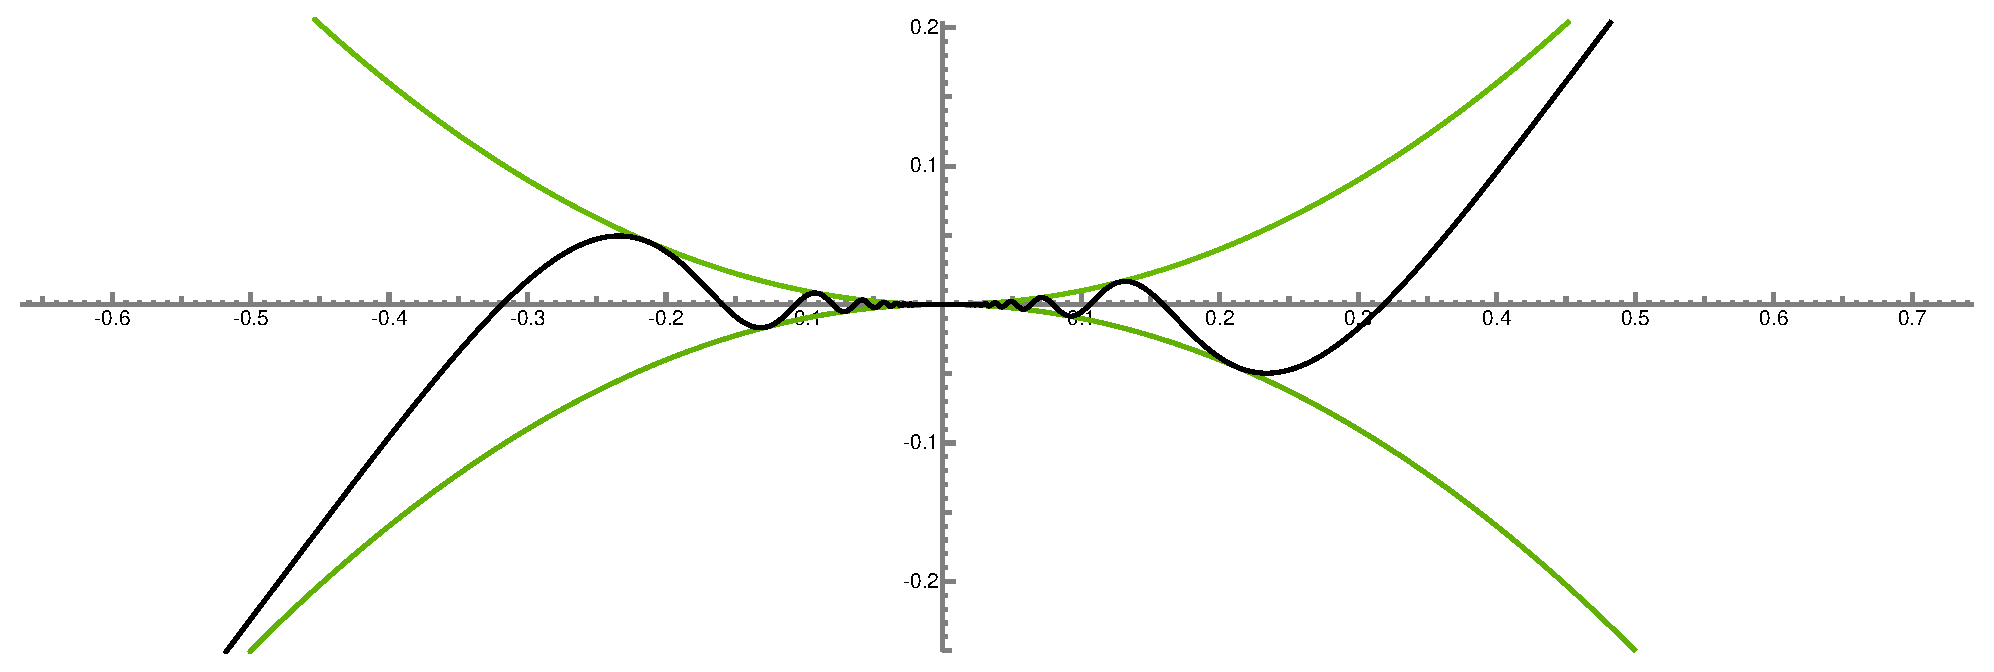
\includegraphics[height=3cm]{darboux.pdf}
  \centering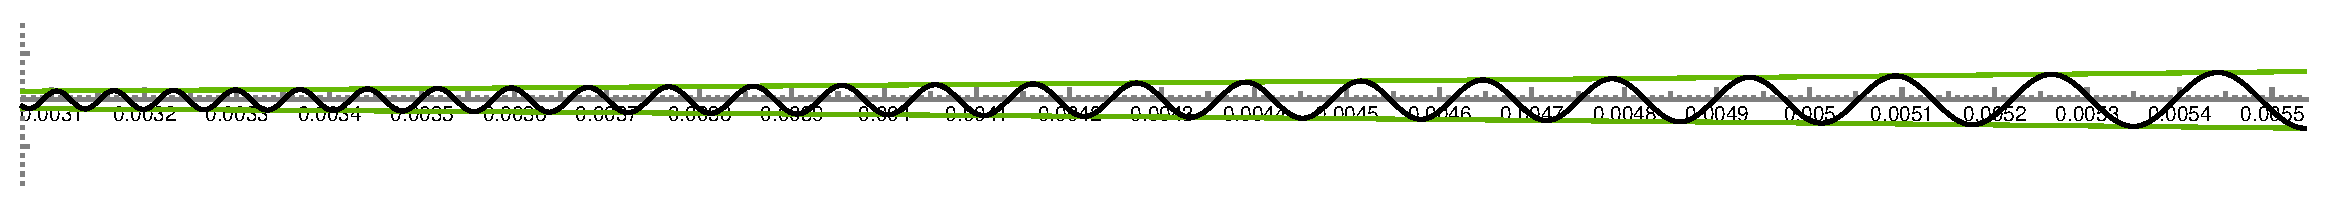
\includegraphics[width=\textwidth]{darboux2.pdf}
  \begin{comment}
  \begin{tikzpicture}[scale=5]
    \draw[->] (-0.5, 0) -- (0.5, 0) node[above] {$x$};
    \draw[->] (0, -0.3) -- (0, 0.3) node[right] {$y$};
    \draw[domain=-0.51:0.5, smooth, variable=\x, gray] plot ({\x}, {\x*\x});
    \draw[domain=-0.51:0.5, smooth, variable=\x, gray] plot ({\x}, {-\x*\x});
    \draw[domain=-0.51:0.5, variable=\x, samples=200, blue, thick] plot ({\x}, {\x*\x*sin(deg(1/\x))});
  \end{tikzpicture}
  \begin{tikzpicture}[scale=5000]
    \draw[->] (0.0045, 0) -- (0.0055, 0) node[above] {$x$};
    \draw[domain=0.0045:0.0055, smooth, variable=\x, gray] plot ({\x}, {\x*\x});
    \draw[domain=0.0045:0.0055, smooth, variable=\x, gray] plot ({\x}, {-\x*\x});
    \draw[domain=0.0045:0.0055, variable=\x, samples=200, blue, thick] plot ({\x}, {\x*\x*sin(deg(1/\x))});
  \end{tikzpicture}
  \end{comment}
  \caption{Il grafico di una funzione derivabile ma con 
    derivata non continua (vedi esempio~\ref{ex:derivata_non_continua}).
    L'ingrandimento nel disegno in basso rende evidente 
    il fatto che la derivata oscilla tra i valori 
    $-1$ e $1$ in ogni intorno di $0$.
    La proprietà di Darboux (teorema~\ref{th:darboux})
    rimane comunque soddisfatta: la derivata assume tutti i valori 
    compresi tra $1$ e $-1$ in ogni intorno di $x=0$ ma 
    non ha limite per $x\to 0$.
}
\end{figure}

\begin{example}
[funzione derivabile con derivata non continua]
\label{ex:derivata_non_continua}%
\mymark{**}%
\index{funzione!derivabile con derivata non continua}%
\index{derivata!non continua}%
La funzione $f\colon \RR \to \RR$ definita da
\[
  f(x)
  = \begin{cases}
    x^2 \sin(1/x) & \text{se $x \neq 0$} \\
    0 & \text{se $x=0$.}
  \end{cases}
\]
è derivabile su tutto $\RR$, $f'(0)=0$ ma il limite
\[
\lim_{x\to 0} f'(x)
\]
non esiste (e dunque $f'\colon \RR\to\RR$ non è continua in $x=0$).
\end{example}
%
\begin{proof}
La funzione $x^2 \sin(1/x)$ è derivabile infinite volte su tutto il suo dominio $\RR\setminus\ENCLOSE{0}$ in quanto composizione di funzioni elementari derivabili infinite volte.
Dunque, per la località della derivata, anche la funzione $f$ è derivabile infinite volte su $\RR\setminus\ENCLOSE{0}$.
Per $x\neq 0$ possiamo quindi calcolare $f'(x)$ utilizzando le regole di derivazione
\[
  f'(x)
  = D \enclose{x^2\sin \frac 1 x}
  = 2x \sin \frac 1 x + x^2 \enclose{\cos \frac 1 x} \cdot\frac{-1}{x^2}
  = 2x \sin \frac 1 x - \cos \frac 1 x.
\]

Verifichiamo ora che $f$ è continua e derivabile anche in $0$.
Si ha infatti
\[
 \lim_{h\to 0}\frac{f(0+h)-f(0)}{h}
 = \lim_{h\to 0} h \sin \frac 1 h = 0
\]
e dunque $f'(0) = 0$.
Osserviamo però che $f'(x)$ non ammette limite per $x\to 0$
in quanto per $x \to 0$ si ha $2x \sin(1/x) \to 0$ ma il limite di $\cos (1/x)$ invece non esiste. Dunque $f'(x)$ è la somma di una funzione che ha limite zero e di una funzione il cui limite non esiste per $x\to 0$. Dunque $f'(x)$ non ammette limite per $x\to 0$.
\end{proof}

\begin{proposition}[criterio di derivabilità]
\label{prop:4384774}\mymark{**}
Sia $I\subset \RR$ un intervallo, $x_0\in I$
$f\colon I \to \RR$ una funzione continua su tutto $I$ e derivabile in $I\setminus\ENCLOSE{x_0}$.
Se il limite della derivata
\[
  \lim_{x\to x_0} f'(x) = m
\]
esiste ed è finito la funzione $f$ è derivabile anche in $x_0$ e vale $f'(x_0) = m$.
\end{proposition}
%
\begin{proof}
\mymark{*}
Prendiamo un generico punto $x>x_0$ (il caso $x<x_0$ è del tutto analogo).
Per il teorema
di Lagrange sappiamo esistere un punto $y\in (x_0,x)$ tale che
\[
  \frac{f(x)-f(x_0)}{x-x_0} = f'(y).
\]
Per $x\to x_0$ si ha certamente anche $y\to x_0$ e dunque
esiste il limite del rapporto incrementale:
\[
  f'(x_0) = \lim_{x\to x_0} \frac{f(x)-f(x_0)}{x-x_0}
  = \lim_{y\to x_0} f'(y) = m.
\]
\end{proof}
%
La proposizione precedente dice che la derivata di una funzione in un
punto non può avere un valore diverso dal suo limite, se tale limite esiste.
Esistono però funzioni derivabili la cui derivata non è
continua, come abbiamo visto
nell'esempio~\ref{ex:derivata_non_continua}
in quanto il limite della derivata potrebbe non esistere.


\section{convessità}

\begin{definition}[funzione convessa]
\mymark{**}
Sia $I\subset \RR$ un intervallo.
Una funzione $f\colon I\to \RR$
si dice essere
\emph{convessa}
\mynote{funzione convessa}
\index{funzione!convessa}
se per ogni $x,y\in I$ e per ogni $t\in [0,1]$ si ha
\[
f((1-t)x + ty) \le (1-t) f(x) + t f(y).
\]

Analogamente diremo che $f$ è \emph{concava} \mynote{funzione concava}
\index{funzione!concava}
se vale la disuguaglianza inversa:
\[
f((1-t)x + ty) \ge (1-t) f(x) + t f(y)
\]
(o, equivalentemente, se $-f$ è convessa).
\end{definition}

Osserviamo che la retta del piano passante per i punti $(x,f(x))$ e $(y,f(y))$ può essere parametrizzata in maniera uniforme per $t\in \RR$
da
\[
  (1-t) (x,f(x)) + t(y,f(y)) = ((1-t)x + ty, (1-t) f(x) + tf(y)).
\]
Chiaramente per $t=0$ si ottiene il punto $(x,f(x))$ per $t=1$ il punto $(y,f(y))$ e per $t\in[0,1]$ il segmento congiungente tali punti. La condizione di convessità della funzione $f$ corrisponde quindi a richiedere che ogni corda (segmento) che unisce due punti del grafico si trovi "al di sopra" del grafico della funzione.

\begin{definition}[insieme convesso]
\mymark{*}
Un insieme $E\subset \RR^n$ si dice essere \myemph{convesso} se dati
due punti qualunque $a,b\in E$ l'intero segmento $[a,b]=\ENCLOSE{(1-t)a+tb\colon t\in [0,1]}$ è contenuto in $E$.
\end{definition}

\begin{theorem}[epigrafico delle funzioni convesse]
Sia $I\subset \RR$ e $f\colon I\subset \RR\to \RR$ una funzione.
Allora sono equivalenti:
\begin{enumerate}
\item $I$ è un intervallo e $f$ è convessa;
\item l'\myemph{epigrafico di $f$} (o \emph{sopragrafico})
\index{epigrafico}
ovvero l'insieme
\[
  E = \ENCLOSE{(x,y)\in \RR^2\colon x\in I, y\ge f(x)}
\]
è convesso.
\end{enumerate}

Per le funzioni concave sarà il \emph{sottografico} $\ENCLOSE{(x,y)\colon y\le f(x)}$ ad essere convesso.
\end{theorem}
%
\begin{proof}
Supponiamo che $I$ sia un intervallo e $f$ sia convessa. Per dimostrare che l'epigrafico $E$ è convesso consideriamo due punti $a,b\in E$ e un qualunque punto $p$ sul segmento $[a,b]$.
Se $a=(x_a, y_a)$, $b=(x_b,y_b)$, $p=(x_p, y_p)$
allora esiste un $t\in [0,1]$ tale che $x_p = (1-t)x_a + t x_b$ e $y_p=(1-t)y_a + t y_b$.
Visto che $a,b\in E$ sappiamo che $y_a \ge f(x_a)$ e $y_b\ge f(x_b)$. Dunque necessariamente si ha
\[
  y_p \ge (1-t)f(x_a) + t f(y_b).
\]
Ma essendo $f$ convessa si ha:
\[
  (1-t)f(x_a) + t f(y_b) \ge f((1-t)x_a + t x_b) = f(x_p).
\]
Dunque $y_p\ge f(x_p)$ che significa $p\in E$.

Viceversa supponiamo di sapere che $E$ è convesso. Siano $x,y\in I$ punti qualunque. Allora i punti $a=(x,f(x))$ e $b=(y,f(y))$ sono certamente punti di $E$ e quindi l'intero segmento $[a,b]$ deve essere contenuto in $E$. Dunque per ogni $t\in [0,1]$ il punto $p = ((1-t)x + t y,$ $(1-t)f(x)+ tf(y))$ deve stare in $E$. In primo luogo deve quindi essere $(1-t)x+ty\in I$ e se questo è vero per ogni $t\in[0,1]$ significa che $I$ è un intervallo. In secondo luogo se $p\in E$ significa che
\[
  (1-t)f(x) +t f(y) \ge f((1-t)x + t y)
\]
che corrisponde alla definizione di funzione convessa.
\end{proof}


\begin{lemma}[rapporto incrementale di una funzione convessa]
\mymark{*}%
\label{lemma:547091}%
Sia $I$ un intervallo di $\RR$ e sia $f\colon I\to \RR$.
Dati $x,y\in I$ con $x\neq y$ definiamo il \emph{rapporto incrementale}
di $f$ come:
\[
  R(x,y) = \frac{f(y) - f(x)}{y-x}.
\]
Allora sono condizioni equivalenti:
\begin{enumerate}
\item $f$ è convessa;
\item per ogni $x,y,z\in I$ se $x<y<z$ si ha $R(x,y)\le R(y,z)$;
\item per ogni $x,y,z\in I$ se $x<y<z$ si ha $R(x,y)\le R(x,z)$;
\item per ogni $x,y,z\in I$ se $x<y<z$ si ha $R(x,z)\le R(y,z)$;
\item la funzione $R(x,y)$ è crescente in ognuna delle due variabili.
\end{enumerate}
\end{lemma}
%
\begin{proof}
Attenzione:
il lemma risulta ovvio se si utilizza la giusta interpretazione geometrica
(il rapporto incrementale è la pendenza della corda corrispondente).
Quella che segue è la traduzione algebrica di quanto
è geometricamente ovvio ma risulta inevitabilmente pesante
e più difficilmente comprensibile.

Siano $x,y,z\in I$ con $x<y<z$.
Posto $t=(y-x)/(z-x)$ si ha $y=(1-t)x + tz$,
 $y-x = t(z-x)$, $z-y = (1-t)(z-x)$.
Si ha allora
 \begin{equation*}
 \begin{aligned}
 R(x,z) - R(x,y)
 &= \frac{f(z)-f(x)}{z-x} - \frac{f(y)-f(x)}{y-x} \\
  &= t\frac{f(z)-f(x)}{y-x} - \frac{f(y)-f(x)}{y-x} \\
  &= \frac{tf(z) + (1-t) f(x) - f(y)}{y-x}
 \end{aligned}
 \end{equation*}

La condizione di convessità di $f$ è
\[
  f(y) \le (1-t)f(x) + tf(z)
\]
ed è quindi equivalente alla condizione $R(x,y) \le R(x,z)$.
Dunque le condizioni 1 e 3 sono equivalenti.

Ma con una verifica diretta si osserva che
\[
  R(x,z) = t R(x,y) + (1-t) R(y,z)
\]
da cui si ottiene
\[
  R(y,z) - R(x,z) = t[R(y,z) - R(x,y)]
\]
oppure anche
\[
 R(x,z) - R(x,y) = (1-t) [R(y,z) - R(x,y)].
\]
Risulta quindi che le quantità
\[
  R(y,z) - R(x,y), \qquad
  R(x,z) - R(x,y), \qquad
  R(y,z) - R(x,z)
\]
hanno tutte lo stesso segno. E quindi le condizioni 2, 3 e 4 sono tra loro equivalenti (se vale una delle tre valgono tutte e tre).

Se valgono le tre condizioni 2, 3 e 4 è facile verificare che la funzione $R(x,y)$ è crescente in entrambe le variabili. Innanzitutto per simmetria, visto che $R(x,y) = R(y,x)$, è sufficiente verificare che $R(x,y)$ è crescente nella seconda variabile $y$ per ogni $x$ fissato. Quindi dato $z>y$ bisogna mostrare che $R(x,z) \ge R(x,y)$.
Abbiamo allora tre possibilità a seconda che sia $x<y$ oppure $y<x<z$ oppure $z<x$. Nel primo caso si ha $x<y<z$ e dunque la disuguaglianza $R(x,y) \le R(x,z)$ corrisponde alla condizione 3.
Nel secondo caso si ha $y<x<z$ e la condizione $R(x,y)\le R(x,z)$ si può scrivere come $R(y,x) \le R(x,z)$ che è, riordinando opportunamente le variabili, la condizione 2. Se, infine, $y < z < x$ la condizione $R(x,y) \le R(x,z)$ si può scrivere $R(y,x) \le R(z,x)$ che, riordinando le variabili, è la condizione 4.

Viceversa (e infine) se la funzione $R(x,y)$ è crescente in entrambe le variabili in particolare è crescente nella seconda variabile e quindi se $x<y<z$ si ha $R(x,y) \le R(x,z)$. Risulta quindi che la condizione 5 implica la 3 e quindi tutte le altre condizioni.
\end{proof}

\begin{theorem}
\mymark{***}
Sia $I\subset \RR$ un intervallo e $f\colon I \to \RR$ una funzione derivabile su tutto $I$.
Allora sono equivalenti:
\begin{enumerate}
\item $f$ è convessa;
\item per ogni $x_0 \in I$ e per ogni $x\in I$ si ha
\[
   f(x) \ge f'(x_0) (x-x_0) + f(x_0)
\]
(geometricamente: il grafico della funzione sta sopra la retta tangente);
\item $f'$ è crescente.
\end{enumerate}

Analogamente per le funzioni concave si avrà che il grafico ``sta sotto'' la retta tangente e che la derivata è decrescente.
\end{theorem}
%
\begin{proof}
\mymark{**}
Osserviamo che
\[
  f'(x_0) = \lim_{x\to x_0} R(x_0,x).
\]
Se $f$ è convessa allora, per il lemma, il rapporto incrementale $R(x_0,x)$ è crescente e quindi  $f'(x_0) = \inf_{x>x_0} R(x_0,x)$. In particolare $f'(x_0) \le R(x_0,x)$ per ogni $x> x_0$. In maniera analoga si trova $f'(x_0) \ge R(x_0,x)$ se $x<x_0$.
In ogni caso risulta quindi che per ogni $x$ si ha
\[
(R(x_0,x)- f'(x_0))(x-x_0)\ge 0
\]
ovvero
\[
  f(x) - f(x_0) - f'(x_0)(x-x_0) \ge 0.
\]
Dunque la condizione 1 implica la 2.

Se vale la condizione 2, dati $x,y \in I$ si ha
\[
  f(x) - f(y) \ge f'(y)(x-y)
\]
se scambiamo $x$ e $y$ e cambiamo di segno ambo i membri si ottiene invece
\[
  f(x) - f(y) \le f'(x)(x-y)
\]
mettendo insieme le due disuguaglianze,
se ora supponiamo che sia $x>y$ otteniamo proprio
$f'(x) \ge f'(y)$ cioè $f'$ è crescente (condizione 3).

Supponiamo ora di sapere che $f'$ è crescente e supponiamo per assurdo che la funzione $f$ non sia convessa.
In base al lemma precedente dovrebbero allora esistere tre punti $x<y<z$ tali che $R(x,y)> R(y,z)$. Per il teorema di Lagrange dovrebbe allora esistere un punto $c\in (x,y)$ tale che $f'(c) = R(x,y)$ e un punto $d \in (y,z)$ tale che $f'(d) = R(y,z)$ ma allora
$f'(c) > f'(d)$ nonostante sia $c<d$ e dunque $f'$ non poteva essere crescente.
\end{proof}

\begin{corollary}[criterio di convessità tramite derivata seconda]
\mymark{***}
Sia $I\subset \RR$ un intervallo e sia $f\colon I \to \RR$ una funzione derivabile due volte (cioè $f$ è derivabile e anche $f'$ è derivabile).
Allora $f$ è convessa se e solo se $f''(x)\ge 0$ per ogni $x\in I$.
Analogamente $f$ è concava se e solo se $f''\le 0$.
\end{corollary}
\begin{proof}
\mymark{***}
Per il criterio precedente $f$ è convessa se e solo se $f'$ è crescente. Per il criterio di monotonia $f'$ è crescente se e solo se $f'' \ge 0$. Considerazioni analoghe valgono per la concavità.
\end{proof}

\begin{theorem}
Siano $a\in \RR$, $b\in \bar \RR$, $a<b$.
Sia $f\colon [a,b)\to \RR$ una funzione convessa in $(a,b)$ e continua in $a$. Allora $f$ è convessa su tutto $[a,b)$. Risultato analogo vale per funzioni definite su intervalli aperti a sinistra $(a,b]$
e aperti da ambo i lati $(a,b)$.
\end{theorem}
%
\begin{proof}
Dati $x,y \in [a,b)$ dobbiamo mostrare che per ogni $t\in[0,1]$ vale
\[
f((1-t) x+ t y) \le (1-t)f(x) + t f(y).
\]
Per ipotesi sappiamo che la disuguaglianza è valida se $x,y \in (a,b)$. Dobbiamo quindi dimostrare la disuguaglianza solamente nel caso $x=a$ e $y\in(a,b)$. Dato qualunque $t\in (0,1)$ e
presa una successione $x_k \to a$ con $x_k\in (a,b)$ definiamo
$t_k$ in modo che sia $z = (1-t)x + ty = (1-t_k) x_k + t_k y$
cioè:
\[
  t_k = \frac{x - x_k + t(y-x)}{y-x_k}.
\]
Siccome $t_k\to t$ per $k\to +\infty$ se $t\in (0,1)$ per $k$ abbastanza grande anche $t_k\in(0,1)$. Inoltre per la convessità in $(a,b)$ sappiamo che vale
\[
  f((1-t_k)x_k + t_k y) \le (1-t_k) f(x_k) + t_k f(y)
\]
e passando a limite per $k\to +\infty$, dalla continuità di $f$ in $x$ si ottiene
\[
   f((1-t)x+ty) \le (1-t) f(x) + t f(y)
\]
come volevamo dimostrare. Per $t=0$ e $t=1$ la disuguaglianza è sempre banalmente verificata.
\end{proof}

\begin{example}
La funzione $f(x) = \sqrt{x}$ è definita su $[0,+\infty)$ ma è derivabile solamente in $(0,+\infty)$. La sua derivata è $f'(x) = x^{-\frac 1 2 }/2$ e la derivata seconda è $f''(x) = -x^{-\frac 3 2}/4 < 0$. Dunque la funzione è concava sull'intervallo aperto $(0,+\infty)$. Ma essendo continua possiamo concludere che $f$ è concava su tutto il dominio $[0,+\infty)$.
\end{example}

\begin{comment}
\begin{theorem}[continuità delle funzioni convesse]
Siano $a,b \in \bar \RR$ con $a< b$.
Sia $f\colon (a,b) \to \RR$ una funzione convessa. Allora $f$ è continua.
\end{theorem}
%
\begin{proof}
Sia $x_0 \in (a,b)$ e siano $y,z \in (a,b)$ con $y < x_0 < z$.
Per il lemma sui rapporti incrementali sappiamo che per ogni $x\in (y,z)$ si ha
\[
   R(x_0, y) \le R(x_0,x) \le R(x_0,z).
\]
In particolare esiste una costante $C$ tale che
\[
  \abs{R(x_0,x)} \le C,\qquad \forall x \in (y,z).
\]
Moltiplicando per $\abs{x-x_0}$ si ottiene allora
\[
   \abs{f(x) - f(x_0)} \le C \abs{x-x_0}
\]
e per $x\to x_0$ il lato destro tende a zero e quindi per confronto anche il lato sinistro deve tendere a zero. Dunque $f(x)\to f(x_0)$
e $f$ è continua in $x_0$.
\end{proof}
\end{comment}

\begin{theorem}[derivabilità delle funzioni convesse]
  Sia $I\subset \RR$ un intervallo e sia $f\colon I \to \RR$ una funzione convessa.
  Se $x_0\in (\inf I, \sup I)$ esistono e sono finite la derivata destra 
  e sinistra di $f$ in $x_0$:
  \begin{align*}
    f'_+(x_0) &= \lim_{x\to x_0^+} \frac{f(x)-f(x_0)}{x-x_0}\\
    f'_-(x_0)  &= \lim_{x\to x_0^-} \frac{f(x)-f(x_0)}{x-x_0}  
  \end{align*}
  e risulta
  \[
    f'_-(x_0) \le f'_+(x_0).
  \]
  Inoltre se $\inf I < x_1 < x_2 < \sup I$ si ha 
  \[
    f'_+(x_1) \le f'_(x_2).
  \]
  Se ne deduce che $f$ è continua in tutti i punti interni di $I$ 
  e che l'insieme dei punti in cui $f$ non è derivabile 
  è al più numerabile.
  \end{theorem}
  %
  \begin{proof}
    Nel lemma~\ref{lemma:547091} abbiamo osservato che il rapporto incrementale
    \[
      R(x_0,x) = \frac{f(x)-f(x_0)}{x-x_0}
    \] 
    di una funzione convessa è crescente rispetto alla variabile $x$. 
    Dunque per il teorema~\ref{th:limite_monotona} si 
    ha 
    \[
      f'_-(x_0) = \sup_{x<x_0} R(x_0,x)>-\infty, \qquad 
      f'_+(x_0) = \inf_{x>x_0} R(x_0,x)<+\infty
    \]
    e visto che se $x<x_0$ e $y>x_0$ si ha $R(x_0,x)\le R(x_0,y)$ 
    deduciamo che $f'_-(x_0)\le f'_+(x_0)$ ed entrambi i limiti 
    sono dunque finiti. Se $x_1 < x_2$ allora preso un qualunque 
    punto $x$ con $x_1<x<x_2$ si ha (sempre per il lemma~\ref{lemma:547091})
    \[
      R(x_1,x) \le R(x,x_2)
    \]
    e dunque passando al limite si trova $f'_+(x_1) \le f'_-(x_2)$.
    Le derivate destra e sinistra esistono dunque in tutti i punti interni 
    all'intervallo $I$. 
    In particolare $f$ è continua in tali punti in quanto è continua sia da destra 
    che da sinistra.
    I punti di non derivabilità di $f$ sono i punti in cui 
    le derivate destra e sinistra differiscono. 
    Ma ad ogni punto $x$ di non differenziabilità 
    posso associare l'intervallo aperto non vuoto $I_x = (f'_-(x),f'_+(x))$ e per 
    le proprietà appena viste è chiaro che questi intervalli sono a due a due disgiunti
    in quanto se $x_1<x_2$ l'estremo destro di $I_{x_1}$ è minore o uguale all'estremo 
    sinistro di $I_{x_2}$.
    Siccome ognuno di questi intervalli contiene almeno un numero razionale concludiamo che 
    il numero di punti di discontinuità non può essere maggiore della cardinalità 
    dei numeri razionali.
  \end{proof}
  
  \begin{theorem}[retta di supporto]
    \label{th:supporto_convessa}%
    Sia $I\subset \RR$ un intervallo, $f\colon I\to\RR$ una funzione convessa 
    e $x_0$ un punto interno ad $I$. Allora esiste una funzione lineare affine 
    \[
      L(x) = mx+q
    \]
    tale che $f(x_0) = L(x_0)$ e per ogni $x\in I$ si abbia $f(x)\ge L(x)$.
  \end{theorem}
  %
  \begin{proof}
    Basta scegliere qualunque $m\in [f'_-(x_0),f'_+(x_0)]$ e considerare la funzione 
    lineare affine $L(x) = m(x-x_0)$. Se $x>x_0$ allora si ha $R(x_0,x)\ge m$ 
    e dunque $f(x) - f(x_0) \ge m (x-x_0) = L(x)$. Viceversa se $x<x_0$ 
    si ha $R(x_0,x)\le m$ da cui, di nuovo, $f(x)-f(x_0) \ge m(x-x_0) = L(x)$.
  \end{proof}
  %
  Il seguente teorema può essere enunciato anche per gli integrali 
  come vedremo nel teorema~\ref{th:jensen}. 
  La dimostrazione è sostanzialmente identica ed è valida anche 
  per funzioni convesse di più variabili.
  %
  \begin{theorem}[combinazioni baricentriche/disuguaglianza di Jensen]
    \mymark{*}%
    \label{th:combinazioni_baricentriche}%
    \index{combinazioni baricentriche}%
    \index{disuguaglianza!di Jensen}%
    \index{Jensen!disuguaglianza di}%
    Se $f$ è una funzione convessa definita su un intervallo $I$, dati $x_1, \dots, x_n \in I$ e $\lambda_1, \dots, \lambda_n\in \RR$ tali che $\sum_{k=1}^n \lambda_k = 1$ e $\lambda_k \ge 0$ per ogni $k=1, \dots, n$ allora
    \[
      f\enclose{\sum_{k=1}^n \lambda_k x_k}
      \le \sum_{k=1}^n \lambda_k f(x_k).
    \]
    Per le funzioni concave vale la disuguaglianza inversa.
    \end{theorem}
    %
    \begin{comment}
    \begin{proof}
    Procediamo per induzione su $n$. Nel caso $n=1$ si ha $\lambda_1=1$ e i due lati della disuguaglianza sono effettivamente uguali. Supponendo il teorema dimostrato per un certo $n$, procediamo a dimostrarlo per $n+1$.
    Osserviamo che
    \begin{align*}
      \sum_{k=1}^{n+1} \lambda_k x_k
      &= \sum_{k=1}^n \lambda_k x_k  + \lambda_{n+1} x_{n+1} \\
      &= (1-\lambda_{n+1})\sum_{k=1}^n\frac{\lambda_k}{1-\lambda_{n+1}} x_k + \lambda_{n+1} x_{n+1}.
    \end{align*}
    Visto che
    \[
      \sum_{k=1}^{n+1} \lambda_k = 1
    \]
    si ha
    \[
      \sum_{k=1}^n \frac{\lambda_k}{1-\lambda_{n+1}}
      = \frac{1-\lambda_{n+1}}{1-\lambda_{n+1}} = 1.
    \]
    Dunque, per ipotesi induttiva si ha allora
    \[
      f\enclose{\sum_{k=1}^n\frac{\lambda_k}{1-\lambda_{n+1}} x_k}
      \le \sum_{k=1}^n \frac{\lambda_k}{1-\lambda_{n+1}}f(x_k).
    \]
    Usando di nuovo la convessità di $f$ con $t=\lambda_{n+1}$ si ha
    \begin{align*}
    f\enclose{\sum_{k=1}^{n+1} \lambda_k x_k}
    &=f\enclose{(1-\lambda_{n+1})\sum_{k=1}^n \frac{\lambda_k}{1-\lambda_{n+1}}x_k + \lambda_{n+1}x_{n+1}}\\
    &\le (1-\lambda_{n+1})f\enclose{\sum_{k=1}^n \frac{\lambda_k}{1-\lambda_{n+1}}x_k} + \lambda_{n+1}f(x_{n+1}) \\
    &\le (1-\lambda_{n+1})\sum_{k=1}^n \frac{\lambda_k}{1-\lambda_{n+1}} f(x_k) + \lambda_{n+1} f(x_{n+1})\\
    &= \sum_{k=1}^{n+1}\lambda_k f(x_k).
    \end{align*}
    come volevamo dimostrare.
    \end{proof}
  \end{comment}
  %    
  \begin{proof}
  Poniamo 
  \[
    \bar x =  \sum_{k=1}^n \lambda_k x_k.
  \]
  Per il teorema~\ref{th:supporto_convessa} precedente 
  sappiamo che esiste una retta $L(x) = mx + q$ 
  tale che $L(\bar x) = f(\bar x)$ 
  e $L(x)\le f(x)$ per ogni $x \in I$.
  Allora si ha 
  \[
  L \enclose{\sum_{k=1}^n \lambda_k x_k}
  = \sum_{k=1}^n m \lambda_k x_k + q \sum_{k=1}^n \lambda_k 
  = \sum_{k=1}^n \lambda_k L(x_k).  
  \]
  Dunque 
  \[
  f(\bar x) = L(\bar x) = \sum_{k=1}^n \lambda_k L(x_k) \le 
  \sum_{k=1}^n \lambda_k f(x_k).
  \]
  \end{proof}

\begin{example}[disuguaglianza tra media aritmetica e media geometrica]
\mymark{*}
\index{disuguaglianza!media aritmetica media geometrica}
Osserviamo che la funzione $f(x) = \ln x$ è concava, infatti si ha
$f''(x) = -1/x^2 < 0$. Dunque, per il teorema precedente, se $\lambda_1 + \dots + \lambda_n =1$, $\lambda_k \ge 0$ si ha
\[
    \ln\enclose{\sum_{k=1}^n \lambda_k x_k}
    \ge \sum_{k=1}^n \lambda_k \ln x_k.
\]
Facendo l'esponenziale di ambo i membri si ottiene
\[
  \sum_{k=1}^n \lambda_k x_k \ge \prod_{k=1}^n x_k^{\lambda_k}.
\]
Nel caso particolare $\lambda_k = 1/n$ si ottiene
la disuguaglianza tra \emph{media aritmetica} (AM per gli anglofoni)
e \emph{media geometrica}
\mymargin{media aritmetica geometrica}%
\index{media!aritmetica}%
\index{media!geometrica}%
\index{AM}%
\index{GM}%
(GM):
\[
  \frac{x_1 + \dots + x_n}{n} \ge \sqrt[n]{x_1\cdots x_n}.
\]
\end{example}

\begin{exercise}[subadditività delle funzioni concave]
Sia $f\colon [0,+\infty) \to \RR$ una funzione concava con $f(0)\ge 0$. Allora $f$ è subadditiva cioè:
\[
  f(x+y) \le f(x) + f(y),\qquad \forall x,y\ge 0.
\]
\end{exercise}
%
\begin{proof}
Se $x=y=0$ la disuguaglianza è ovvia.
Altrimenti $x+y>0$ e si ha
\begin{align*}
f(x) &= f\enclose{\frac{y}{x+y}\cdot 0 + \frac{x}{x+y}\cdot (x+y)}\\ &\ge \frac{y}{x+y}f(0) + \frac{x}{x+y}f(x+y)
\ge \frac{x}{x+y}f(x+y).
\end{align*}
Scambiando $x$ con $y$ e sommando si ottiene:
\[
  f(x) + f(y) \ge \frac{x}{x+y}f(x+y) + \frac{y}{x+y}f(x+y) = f(x+y).
\]
\end{proof}

Si osservi che sviluppando la disuguaglianza $(x-y)^2\ge 0$ si ottiene:
\[
  x y \le \frac{x^2 + y^2}{2}.
\]
Questa disuguaglianza può essere generalizzata ad esponenti diversi 
come si vede nel seguente.

\begin{theorem}[disuguaglianza di Young]%
\label{th:young}%
\index{Young!disuguaglianza di}%
\index{disuguaglianza!di Young}%
Se $p>1$, $q>1$, $\frac{1}{p}+\frac{1}{q}=1$, $x,y\ge 0$:
\begin{equation}\label{eq:young}
  x y \le \frac{x^p}{p} + \frac{y^q}{q}.
\end{equation}
\end{theorem}
%
\begin{proof}
Si utilizza la disuguaglianza di convessità per la funzione $\exp(x)=e^x$. 
Visto che la derivata seconda dell'esponenziale è positiva, la funzione $\exp$ 
è convessa e dunque, se $x>0$ e $y>0$ si ha:
\begin{align*}
 x\cdot y 
  &= \exp(\ln x + \ln y)
  = \exp\enclose{\frac 1 p \ln (x^p) + \frac 1 q \ln (y^q)}  \\
  &\le \frac 1 p \cdot \exp \ln (x^p) + \frac 1 q \exp \ln (y^q)
  = \frac{x^p}{p} + \frac{y^q}{q}.
\end{align*}
Se $x=0$ o $y=0$ la disuguaglianza è ovvia in quanto il lato sinistro 
di~\eqref{eq:young} è nullo.
\end{proof}

\begin{theorem}[disuguaglianza di Hölder]
Se $a_k\ge 0$ e $b_k\ge 0$ per $k\in \NN$
e siano $p>1$ e $q>1$ tali che $\frac 1 p + \frac 1 q = 1$.
Allora 
\[
 \sum_k a_k b_k  \le \enclose{\sum_k a_k^p}^{1 \over p} \cdot \enclose{\sum_k b_k^q}^{1\over q}.
\]
\end{theorem}
\begin{proof}
Poniamo 
\[
A = \enclose{\sum_k a_k^p}^{1 \over p}, \qquad 
B = \enclose{\sum_k b_k^q}^{1\over q}.
\]
Se $A>0$ e $B>0$ possiamo dividere il lato sinistro della disuguaglianza 
per il lato destro e applicare la disuguaglianza~\eqref{eq:young} di Young:
\begin{align*}
  \frac{\sum_k a_k b_k}{A\cdot B} 
  & = \sum_k \frac{a_k}{A}\cdot \frac{b_k}{B} 
  \le \sum_k \frac 1 p \frac{a_k^p}{A^p} + \frac 1 q \frac{b_k^q}{B^q} \\
  &= \frac 1 p \frac{\sum_k a_k^p}{A^p} + \frac 1 q \frac{\sum_k b_k^q}{B^q}
  = \frac 1 p + \frac 1 q = 1.
\end{align*}
E il teorema e dimostrato. 

Se fosse $A=0$ tutti i termini $a_k$ sarebbero nulli e la disuguaglianza 
si riduce banalmente a $0\le 0$. Lo stesso se fosse $B=0$.  
\end{proof}

Nel caso $p=q=2$ si ottiene la 
\myemph{disuguaglianza di Cauchy-Schwarz}
\index{disuguaglianza!di Cauchy-Schwarz}%
\index{Cauchy-Schwarz!disuguaglianza di}%
\index{Schwarz!disuguaglianza di Cauchy-}%
\[
   \sum_k \abs{a_k b_k} \le \sqrt{\sum_k a_k^2} \cdot \sqrt{\sum_k b_k^2}
\]
che potrebbe però essere più facilmente dimostrata 
per un generico prodotto scalare, come faremo 
nel teorema~\ref{th:spazio_euclideo}.

\section{teoremi di Cauchy e de l'Hospital}

\begin{theorem}[Cauchy]
\label{th:cauchy}%
\mymark{**}%
\index{teorema!di Cauchy}%
\mymargin{Cauchy}%
Siano $f\colon[a,b]\to \RR$ e $g\colon[a,b]\to \RR$ funzioni continue su tutto $[a,b]$ e derivabili su $(a,b)$.
Supponiamo inoltre che $g'(x)\neq 0$ per ogni $x\in (a,b)$.
Allora $g(b) \neq g(a)$ ed esiste $x_0\in(a,b)$ tale che
\[
  \frac{f'(x_0)}{g'(x_0)} = \frac{f(b)-f(a)}{g(b)-g(a)}.
\]
\end{theorem}
%
\begin{proof}
\mymark{**}
Si consideri la funzione ausiliaria
\[
 h(x) = (g(b)-g(a))f(x) - (f(b)-f(a))g(x).
\]
Per verifica diretta si osserva che
\[
  h(b) = g(b)f(a) - f(b)g(a) = h(a).
\]
Dunque $h$ verifica le ipotesi del teorema di Rolle ed esiste
dunque un punto $x_0\in(a,b)$ per cui $h'(x_0) = 0$.
Essendo però
\[
  h'(x) = (g(b) - g(a)) f'(x) - (f(b)-f(a)) g'(x)
\]
si ottiene
\[
 (g(b)-g(a))f'(x_0) = (f(b) - f(a))g'(x_0).
\]
Per ipotesi sappiamo che $g'(x_0)\neq 0$.
Ma necessariamente anche $g(b) - g(a)\neq 0$ perché altrimenti potremmo applicare il teorema di Rolle alla funzione $g$ e ottenere che $g'$ si annulla in un punto di $(a,b)$, cosa che abbiamo escluso per ipotesi.
Dunque possiamo dividere ambo i membri per $(g(b)-g(a))$ e per $g'(x_0)$ per ottenere l'uguaglianza enunciata nel teorema.
\end{proof}

\begin{theorem}[de l'Hospital $0/0$]
\mymark{***}
Sia $I\subset \RR$ un intervallo, $x_0\in [-\infty,+\infty]$ un punto di accumulazione
di $I$
e siano $f,g \colon I\setminus\ENCLOSE{x_0} \to \RR$ funzioni derivabili.
Supponiamo che sia $g'(x)\neq 0$ per ogni $x\in I\setminus\ENCLOSE{x_0}$.
Se
\[
  \lim_{x\to x_0} f(x) = 0 \qquad \text{e}\qquad \lim_{x\to x_0} g(x) = 0
\]
e se esiste (finito o infinito) il limite
\[
  \ell = \lim_{x\to x_0}\frac{f'(x)}{g'(x)}
\]
allora si ha
\[
  \lim_{x\to x_0} \frac{f(x)}{g(x)} = \ell.
\]
\end{theorem}
%
\begin{proof}
\mymark{**}
Bisognerà distinguere diversi casi a seconda che $x_0$ sia finito o infinito
e che sia un punto interno o un estremo dell'intervallo $I$.
Fatta la dimostrazione nel primo caso tutti gli altri si riconducono ad esso.

\emph{Caso 1:} supponiamo che sia $I=[x_0, b]$. In questo caso possiamo
estendere le funzioni $f$ e $g$ anche nel punto $x_0$ ponendo:
\[
\tilde f(x) =
\begin{cases}
  f(x) & \text{se $x\in (x_0,b]$}\\
  0 & \text{se $x=x_0$,}
\end{cases}
\qquad
\tilde g(x) =
\begin{cases}
  g(x) & \text{se $x\in (x_0,b]$}\\
  0 & \text{se $x=x_0$.}
\end{cases}
\]
Visto che per ipotesi $f(x) \to 0$ e $g(x)\to 0$ per $x\to x_0$ risulta
che $\tilde f$ e $\tilde g$ siano funzioni continue su tutto l'intervallo $[x_0,b]$
inoltre, sempre per ipotesi, sono derivabili nell'intervallo $(x_0,b]$
visto che l'estensione per $x=x_0$ non modifica le derivate negli altri punti.
In particolare le funzioni estese soddisfano le ipotesi del teorema di Cauchy in
ogni intervallo $[x_0,x]$ con $x\in (x_0,b]$, dunque possiamo affermare
che per ogni $x$ esiste $c(x)\in (x_0,x)$ tale che
\[
  \frac{f(x)}{g(x)}
  = \frac{\tilde f(x) - \tilde f(x_0)}
  {\tilde g(x)- \tilde g(x_0)}
  = \frac{\tilde f'(c(x))}{\tilde g'(c(x))}
  = \frac{f'(c(x))}{g'(c(x))}.
\]
Ma essendo $x_0< c(x) < x$ per $x\to x_0$ si ha $c(x)\to x_0$ e quindi,
tramite un cambio di variabile
(Teorema~\ref{th:limite_composta})
possiamo affermare che
\[
    \lim_{x\to x_0} \frac{f(x)}{g(x)}
  = \lim_{x\to x_0}\frac{f'(c(x))}{g'(c(x))}
  = \lim_{x\to x_0}\frac{f'(x)}{g'(x)} = \ell.
\]

\emph{Caso 2:} supponiamo sia $I$ qualunque e $x_0$ finito.
Visto che le funzioni sono definite su $I\setminus\ENCLOSE{x_0}$ possiamo sempre
supporre $x_0\in I$. Inoltre
visto che i limiti dipendono solo dai valori in un intorno del punto $x_0$
possiamo sempre supporre che $I$ sia un intervallo chiuso e limitato.
Nel passo precedente abbiamo fatto il caso in cui $x_0$ era l'estremo
inferiore di $I$, ma allo stesso modo si può fare il caso in cui
$x_0$ è l'estremo superiore. Se invece $x_0$ fosse un punto interno di $I$
possiamo considerare separatamente il limite destro e sinistro e ricondurci
ai casi in cui $x_0$ era un estremo.

\emph{Caso 3:} supponiamo sia $x_0=+\infty$. In tal caso
l'intervallo $I$ contiene un intevallo $[a,+\infty)$ con $a\in\RR$.
Anche in questo caso vogliamo ricondurci al primo caso tramite il cambio
di variabile $t=1/x$. Posto $F(t) = f(1/t)$ e $G(t)= g(1/t)$ si osserva che $F$ e $G$
sono definite sull'intervallo $(0,1/a]$,
tendono a zero per $t\to 0^+$
sono derivabili,
\[
  F'(t) = -\frac{f'(1/t)}{t^2}, \qquad
  G'(t) = -\frac{g'(1/t))}{t^2}
\]
e risulta quindi
\[
  \lim_{t\to 0^+} \frac{F'(t)}{G'(t)}
  = \lim_{t\to 0^+} \frac{f'(1/t)}{g'(1/t)}
  = \lim_{x\to +\infty} \frac{f'(x)}{g'(x)} = \ell.
\]
Quindi applicano il teorema nel caso già dimostrato possiamo affermare che
\[
  \lim_{x\to +\infty} \frac{f(x)}{g(x)} = \lim_{t\to 0^+} \frac{F(t)}{G(t)} = \ell.
\]

\emph{Caso 4:} il caso $x_0 = -\infty$ si svolge in maniera analoga al caso precedente.
\end{proof}

\begin{comment}
%% Vecchia dimostrazione fatta con le successioni
\begin{theorem}[de l'Hospital $0/0$]
\mymark{***}
\index{teorema!di de l'Hospital}
\mymargin{de l'Hospital}
Siano $a,b\in [-\infty,+\infty]$ con $a<b$.
Siano $f,g \colon (a,b)\to \RR$ funzioni derivabili.
Se
\[
 \lim_{x\to a^+} f(x) = 0 \qquad
 \text{e}\qquad
 \lim_{x\to a^+} g(x) = 0,
\]
se $g'(x) \neq 0$ per ogni $x\in (a,b)$
e se esiste il limite
\[
  \ell = \lim_{x\to a^+}\frac{f'(x)}{g'(x)}
\]
allora
si ha
\[
 \lim_{x\to a^+}\frac{f(x)}{g(x)} = \ell.
\]

Risultato analogo si ha facendo i limiti per $x\to b^-$ invece che per $x\to a^+$ e di conseguenza anche nel caso in cui la funzione sia definita su un intervallo ``bucato''
$f\colon (a,b)\setminus\ENCLOSE{x_0} \to \RR$
e si considerino i limiti ``pieni'' per $x\to x_0$.
\end{theorem}
%
\begin{proof}
\mymark{**}
Notiamo innanzitutto che la funzione $g$ può annullarsi al più in un punto di $(a,b)$ in quanto per il teorema di Rolle se si annullasse in due punti anche la derivata si dovrebbe annullare in un punto intermedio, cosa che abbiamo escluso per ipotesi. Eventualmente rimpiazzando l'intervallo $(a,b)$ con un intervallo più piccolo $(a,b')$ possiamo dunque supporre, senza perdere di generalità, che la funzione $g$ non si annulli mai in $(a,b)$.

Consideriamo ora una generica successione $a_k \in (a,b)$, $a_k \to a$. Per il teorema di collegamento tra limiti di funzione e limiti di successione sarà sufficiente dimostrare che $f(a_k)/g(a_k)\to \ell$.

Osserviamo ora che, fissato $k$, per $x\to a$ si ha
\[
\frac{f(a_k) - f(x)}{g(a_k) - g(x)} \to \frac{f(a_k)}{g(a_k)}
\]
in quanto, per ipotesi, $f(x)\to 0$ e $g(x)\to 0$.
Dunque per ogni $k$
possiamo trovare un punto $x_k \in (a,a_k)$ tale che
\[
\abs{\frac{f(a_k) - f(x_k)}{g(a_k) - g(x_k)} - \frac{f(a_k)}{g(a_k)}}
< \frac 1 k.
\]
Ma sull'intervallo $[x_k,a_k]$ possiamo applicare il teorema di Cauchy
e trovare quindi un punto $y_k\in (x_k,a_k)$ tale che
\[
\frac{f(a_k) - f(x_k)}{g(a_k)-g(x_k)} = \frac{f'(y_k)}{g'(y_k)}
\]
ottenendo quindi:
\[
\abs{\frac{f'(y_k)}{g'(y_k)}-\frac{f(a_k)}{g(a_k)}} < \frac 1 k.
\]
Visto che $y_k \in (a,a_k)$ e visto che $a_k \to a$  certamente anche $y_k\to a$ per $k\to +\infty$ e quindi sappiamo, per ipotesi che
\[
  \frac{f'(y_k)}{g'(y_k)} \to \ell, \qquad \text{per $k\to +\infty$}
\]
e visto che la differenza tende a zero, necessariamente si deve avere anche
\[
  \frac{f(a_k)}{g(a_k)} \to \ell.
\]
\end{proof}

\end{comment}
%
\begin{theorem}[de l'Hospital $\cdot/\infty$]
\mymark{*}
\index{teorema!di de l'Hospital}
\mymargin{de l'Hospital}
Siano $a,b\in [-\infty,+\infty]$ con $a<b$.
Siano $f,g \colon (a,b)\to \RR$ funzioni derivabili.
Se
\[
 \lim_{x\to a^+} \abs{g(x)} = +\infty,
\]
se $g'(x) \neq 0$ per ogni $x\in (a,b)$
e se esiste il limite (finito o infinito)
\[
  \ell = \lim_{x\to a^+}\frac{f'(x)}{g'(x)}
\]
allora
si ha
\[
 \lim_{x\to a^+}\frac{f(x)}{g(x)} = \ell.
\]

Risultato analogo si ha facendo i limiti per $x\to b^-$ invece che per $x\to a^+$ e di conseguenza anche nel caso in cui la funzione sia definita su un intervallo ``bucato''
$f\colon (a,b)\setminus\ENCLOSE{x_0} \to \RR$ e si considerino i limiti ``pieni'' per $x\to x_0$.
\end{theorem}
%
\begin{proof}
Supponiamo per assurdo che non si abbia
\[
  \lim_{x\to a^+} \frac{f(x)}{g(x)} = \ell.
\]
Allora, per il teorema di collegamento tra limiti di funzione e limiti di successione, deve esistere una successione $a_k\in (a,b)$, $a_k\to a$ tale che non si abbia
\[
  \lim_{k\to +\infty} \frac{f(a_k)}{g(a_k)} = \ell.
\]
Se la successione $f(a_k) / g(a_k)$ è limitata allora applicando il teorema di Bolzano Weierstrass sappiamo esistere una sottosuccessione
di $a_k$ convergente ad un valore $m\neq \ell$ (se tutte le sottosuccessioni convergessero ad $\ell$ l'intera successione convergerebbe ad $\ell$).
Se invece $f(a_k) / g(a_k)$ non è limitata possiamo estrarre una sottosuccessione che converge a $+\infty$ oppure a $-\infty$. In ogni caso esiste una successione, che chiameremo ancora $a_k$, ed esiste $m\in \bar \RR$ tale che
\[
  \lim_{k \to +\infty} \frac{f(a_k)}{g(a_k)} = m \neq \ell.
\]
Consideriamo ora un intorno $U$ di $m$ e un intorno $V$ di $\ell$ tali che $U\cap V = \emptyset$.
Siccome $f'(x) / g'(x) \to \ell$ per $x\to a$ esiste un $c\in (a,b)$ tale che per ogni $x\in (a,c)$ si ha
\[
  \frac{f'(x)}{g'(x)} \in V.
\]
Consideriamo allora il seguente rapporto incrementale
\begin{align*}
\frac{f(a_k) - f(x)}{g(a_k) - g(x)}
=\frac{\frac{f(a_k)}{g(a_k)}-\frac{f(x)}{g(a_k)}}{1-\frac{g(x)}{g(a_k)}}
\end{align*}
e osserviamo che il lato destro tende a $m$ per $k\to +\infty$ in quanto $f(a_k)/g(a_k) \to m$ e visto che $\abs{g(a_k)}\to +\infty$ si ha $f(x)/g(a_k)\to 0$ e $g(x)/g(a_k) \to 0$.
Dunque esisterà un $k$ per cui il lato destro sta nell'intorno $U$ di $m$. Al lato sinistro possiamo invece applicare il teorema di Cauchy e trovare quindi un punto $y\in(a_k,c)$ per cui tale lato risulti
uguale a $f'(y)/g'(y)$. Ma visto che $y\in (a,c)$ si dovrà avere $f'(y)/g'(y) \in V$. Questo è assurdo in quanto $U\cap V = \emptyset$.
\end{proof}

\section{classi di regolarità}
%
\begin{definition}[funzioni di classe $C^k$]
\mymark{**}
Dato $A\subset \RR$ denotiamo con $\RR^A$ l'insieme di tutte le funzioni $f\colon A \to \RR$.
Per ogni $k\in \NN$ definiamo
$C^k(A) \subset \RR^A$ nel modo seguente:
\mymargin{$C^k$}
\begin{enumerate}
\item se $k=0$ poniamo
\[
  C^0(A) = \ENCLOSE{f\in \RR^A \colon \text{$f$ continua}}.
\]
\item
  se $k>0$ definiamo induttivamente
  \[
  C^{k}(A) = \ENCLOSE{f\in \RR^A \colon \text{$f$ derivabile e $f'\in C^{k-1}(A)$}}.
  \]
\end{enumerate}
Chiaramente se $j\ge k$ si ha $C^j(A) \subset C^k(A)$ dunque $C^k(A)$ è una famiglia decrescente (rispetto all'inclusione insiemistica) ed ha senso definire:
\mymargin{$C^\infty$}
\[
  C^\infty(A) = \ENCLOSE{f\in \RR^A\colon \forall k \in \NN\colon f\in C^k(A)} = \bigcap_{k\in \NN} C^k(A).
\]

Le funzioni $f\in C^k(A)$ sono derivabili $k$ volte.
Utilizziamo la notazione \myemph{$f^{(j)}$} per denotare la $j$-esima derivata
di una funzione $f$.
Dunque avremo
\[
  f^{(0)} = f, \qquad
  f^{(1)} = f', \qquad
  f^{(2)} = f'', \dots
\]
\end{definition}

Abbiamo già osservato che $\RR^A$ è uno spazio vettoriale reale.
Gli spazi $C^k(A)$ per $k=0, \dots, \infty$ sono una famiglia decrescente di sottospazi vettoriali di $\RR^A$.
Infatti sappiamo che la combinazione lineare di funzioni continue è continua e che la combinazione lineare di funzioni derivabili è derivabile.

E' importante osservare che $C^1(A)$ non coincide con l'insieme delle funzioni derivabili su $A$. Infatti abbiamo già visto nell'esempio~\ref{ex:derivata_non_continua} che esistono funzioni derivabili la cui derivata non è continua e quindi tali funzioni, pur essendo derivabili, non sono di classe $C^1$.

\begin{definition}[funzioni lipschitziane]
\mymark{**}
\mynote{funzione lipschitziana}
\index{funzione!lipschitziana}
\index{Lipschitz}
Una funzione $f\colon A\subset \RR \to \RR$ si dice essere \emph{lipschitziana} (o anche $L$-lipschitziana se vogliamo mettere in evidenza la dipendenza da $L$) se esiste $L>0$ tale che
\[
  \abs{f(x) - f(y)} \le L \abs{x-y}\qquad \forall x,y\in A.
\]
La più piccola costante $L$ per la quale è soddisfatta la precedente relazione si chiama \emph{costante di Lipschitz}
\mynote{costante di Lipschitz}
\index{costante!di Lipschitz}
di $f$.
\end{definition}

\begin{theorem}[criterio di Lipschitz]
\mymark{**}
Sia $f\colon A \subset \RR$ una funzione lipschitziana
con costante di Lipschitz $L$.
Se $f$ è derivabile in un punto $x\in A$ allora $\abs{f'(x)}\le L$.
Viceversa se $f\colon I \subset \RR \to \RR$ una funzione derivabile definita su un intervallo $I$
e se esiste $L$ tale che per ogni $x\in I$ si ha $\abs{f'(x)}\le L$ allora $f$ è lipschitziana.
\end{theorem}
%
\begin{proof}
Se $f$ è Lipschitziana significa che il rapporto incrementale è limitato.
Cioè esiste $L>0$ tale che
\[
  \abs{\frac{f(x) - f(y)}{x-y}} \le L \qquad \forall x,y\in A.
\]
Dunque la derivata, che è il limite del rapporto incrementale, se esiste è anch'essa limitata
dalla stessa costante: $\abs{f'(x)}\le L$ per ogni $x \in A$.

Viceversa se la derivata è limitata $\abs{f'(z)}\le L$ per ogni $z \in I$ e se $x,y\in I$ sono punti qualunque,
allora, per il teorema di Lagrange, il rapporto incrementale di $f$ è uguale alla derivata in un punto $z\in(x,y)$:
\[
  \abs{\frac{f(x) - f(y)}{x-y}} = \abs{f'(z)} \le L.
\]
e dunque la funzione è $L$ lipschitziana:
\[
  \abs{f(x)- f(y)} \le L \abs{x-y}.
\]
\end{proof}

\begin{definition}[funzioni Hoelderiane]
Sia $\alpha>0$.
\mynote{funzione hoelderiana}
\index{funzione!hoelderiana}
\index{Hoelder}
Una funzione $f\colon A \subset \RR \to \RR$ si dice essere $\alpha$-Hoelderiana se
esiste una costante $C>0$ tale che
\begin{equation}\label{eq:2964536}
  \abs{f(x) - f(y)} \le C \abs{x-y}^\alpha.
\end{equation}
\end{definition}

\begin{definition}[uniforme continuità]
\mymark{**}%
Una funzione $f\colon A \subset \RR \to \RR$ si dice essere
\emph{uniformemente continua}
\index{uniforme continuità}%
\index{continuità!uniforme}%
\mynote{uniforme continuità}%
se
\[
 \forall \eps>0\colon \exists \delta > 0 \colon
 \forall x,y\in A \colon \abs{x-y} < \delta \implies \abs{f(x)-f(y)} < \eps.
\]
\end{definition}

\begin{theorem}
Ogni funzione lipschitziana è $1$-Hoelderiana (e viceversa).
Ogni funzione $\alpha$-Hoelderiana è uniformemente continua.
Ogni funzione uniformemente continua è continua.
Ogni funzione $\alpha$-Hoelderiana con $\alpha>1$ ha derivata nulla.
\end{theorem}
%
\begin{proof}
Le prime tre affermazioni seguono direttamente dalle definizioni.
Per l'ultima osservazione si noti che se $\alpha>1$ nella
disuguaglianza~\eqref{eq:2964536} si può dividere per $\abs{x-y}$ e
ottenere quindi che il rapporto incrementale tende a zero se $y\to x$.
\end{proof}

\begin{definition}[modulo di continuità]
Sia $f\colon A\subset \RR \to\RR$ una funzione.
Definiamo il \myemph{modulo di continuità} di $f$ come la funzione
$M\colon$ $[0,+\infty) \to [0,+\infty]$ definita da
\[
  M(r) = \sup \ENCLOSE{\abs{f(x)-f(y)}\colon x,y \in A, \abs{x-y} \le r}.
\]
\end{definition}

\begin{theorem}[proprietà del modulo di continuità]
Sia $f\colon A\to \RR$ e sia $M\colon [0,+\infty)\to [0,+\infty)$ il suo
modulo di contintuità.
La funzione $M(r)$ è crescente;

La funzione $f$ è uniformemente continua se e solo se
\[
  \lim_{r\to 0} M(r) = 0.
\]

La funzione $f$ è lipschitziana se e solo se esiste $L$ tale che
\[
  M(r) \le Lr.
\]

La funzione $f$ è $\alpha$-Hoelderiana se e solo se esiste $C$ tale che
\[
  M(r) \le C r^\alpha.
\]
\end{theorem}
%
\begin{proof}
Osserviamo che la condizione
\[
   M(r) \le c
\]
è equivalente a
\[
\forall x,y\in A \colon \abs{x-y}\le r \implies  \abs{f(x)-f(y)} \le c.
\]
La condizione $M(r)\to 0$ per $r \to 0$ significa
\[
 \forall \eps>0\colon \exists \delta>0 \colon \forall r>0\colon r<\delta \implies M(r)<\eps
\]
e diventa quindi la condizione di uniforme continuità.

Le condizioni di lipschitzianità e di $\alpha$-hoelderianità risultano pure immediatamente.
\end{proof}

\begin{theorem}[restrizione / incollamento di funzioni uniformemente continue]
Sia $f\colon A \subset \RR \to \RR$ una funzione uniformemente continua. Se $B\subset A$ la restrizione $f_{|B}$ di $f$ a $B$ è anch'essa uniformemente continua.

Siano $I,J\subset \RR$ intervalli tali che $I\cap J \neq \emptyset$.
Sia $f\colon I \cup J \to \RR$ una funzione. Se $f_{|I}$ e $f_{|J}$ sono uniformemente continue allora $f$ è uniformemente continua.
\end{theorem}
\begin{proof}
La prima parte, sulla restrizione di una funzione uniformemente continua, deriva direttamente dalla definizione:
se una qualunque proprietà vale per ogni $x,y\in A$ allora a maggior ragione vale per ogni $x,y\in B$ quando $B\subset A$.

Vediamo la seconda parte dell'enunciato: supponiamo $f$ sia uniformemente continua su $I$ e su $J$.
Sia dato $\eps>0$ e siano $\delta_1$ e $\delta_2$ i valori di $\delta$ dati dalle condizioni di uniforme continuità di $f$ rispettivamente su $I$ e su $J$. Consideriamo $\delta = \min\ENCLOSE{\delta_1, \delta_2}$.
Siano ora $x,y$ punti qualunque di $I\cup J$ con $\abs{x-y}< \delta$.

Si possono allora avere due casi possibili:
$x$ e $y$ stanno nello stesso intervallo ($I$ o $J$) oppure stanno uno in $I$ e l'altro in $J$.
Nel primo caso essendo $\delta < \delta_1$ e $\delta< \delta_2$ l'uniforme continuità di $f$ su $I$ e su $J$ garantisce che valga in ogni caso $\abs{f(x)-f(y)} < \eps$. Nel secondo caso deve esistere un punto $z \in I\cap J$ che sia un punto intermedio tra $x$ e $y$.
Allora usando la disuguaglianza triangolare:
\[
  \abs{f(x) - f(y)} \le \abs{f(x) - f(z)} + \abs{f(z) - f(y)}
     \le \eps + \eps.
\]
si ottiene dunque (salvo rimpiazzare $\eps$ con $\eps/2$) anche in
questo caso la stima voluta.
\end{proof}

\begin{theorem}[Heine-Cantor]
\mymark{***}
\index{teorema!di Heine-Cantor}
\mynote{Heine-Cantor}
Siano $a,b\in \RR$, $a<b$.
Sia $f\colon [a,b]\to \RR$ una funzione continua.
Allora $f$ è uniformemente continua.
\end{theorem}
%
\begin{proof}
\mymark{***}
Supponiamo per assurdo che $f$ non sia uniformemente continua. Allora
$f$ soddisfa la negazione della proprietà
\[
 \forall \eps>0\colon \exists \delta > 0 \colon
 \forall x,y\in A \colon \abs{x-y} < \delta \implies \abs{f(x)-f(y)} < \eps
\]
che è
\[
 \exists \eps>0\colon \forall \delta > 0 \colon
 \exists x,y \in A \colon \abs{x-y} < \delta \land \abs{f(x)-f(y)} \ge \eps.
\]
Dunque dato $\eps>0$ che soddisfa la precedente proprietà possiamo
prendere $\delta=1/k$
per ogni $k\in \NN$, ottenendo quindi due successioni $x_k$, $y_k$ tali che
\[
  \abs{x_k-y_k} < \frac 1 k \qquad\text{e}\qquad \abs{f(x_k) - f(y_k)} \ge \eps.
\]
Per il teorema di Bolzano-Weierstrass esisterà una sottosuccessione convergente $x_{k_j} \to c$.
Visto che $\abs{x_k-y_k}\to 0$ si dovrà avere anche $y_{k_j}\to c$.
Ma allora, per la continuità di $f$:
\[
 \abs{f(x_{k_j})-f(y_{k_j})} \to \abs{f(c) - f(c)} = 0
\]
in contraddizione con la condizione $\abs{f(x_k)-f(y_k)}\ge \eps$.
\end{proof}

\begin{theorem}[dell'asintoto]
\index{teorema!dell'asintoto}
\mynote{teorema dell'asintoto}
Sia $f\colon [a,+\infty) \to \RR$ una funzione continua e sia $g\colon [a,+\infty) \to \RR$ una funzione uniformemente continua tale che
\[
  \lim_{x\to +\infty} f(x) - g(x) = 0.
\]
Allora anche $f$ è uniformemente continua.

In particolare se $f$ ha un \myemph{asintoto obliquo} ovvero se esistono $m\in \RR$ e $q\in \RR$ tali che
\[
  \lim_{x\to +\infty} f(x) - (mx + q)  = 0
\]
allora $f$, se è continua, è uniformemente continua.

Risultato analogo vale per le funzioni definite su intervalli del tipo $(-\infty,a]$ (facendo i limiti a $-\infty$) e quindi per funzioni definite su tutto $\RR$ (facendo i limiti sia a $+\infty$ che a $-\infty$).
\end{theorem}

\begin{proof}
Per ogni $\eps>0$ esiste $M>a$ tale che $\abs{f(x)-g(x)} < \eps/3$ per ogni $x\ge M$. D'altra parte la funzione $f$, per il teorema di Heine-Cantor, è uniformemente continua su $[a,M+1]$ e dunque esiste $\delta_1>0$ tale che presi $x,y \in [a,M+1]$ con $\abs{x-y}< \delta_1$
si ha $\abs{f(x)-f(y)} < \eps$. D'altra parte $g$ è uniformemente continua su $[M,+\infty)$ e quindi esiste $\delta_2$ tale che dati $x,y\in [M,+\infty)$ con $\abs{x-y} < \delta_2$ si ha $\abs{g(x)-g(y)} < \eps/3$. Ma in quest'ultimo caso si ha:
\begin{align*}
  \abs{f(x)-f(y)} &\le \abs{f(x) - g(x)} + \abs{g(x) - g(y)} + \abs{g(y)-f(y)} \\
  & \le \frac{\eps}{3} + \frac{\eps}{3} + \frac{\eps}{3} = \eps.
\end{align*}
Posto dunque $\delta = \min\ENCLOSE{1, \delta_1, \delta_2}$
scelti comunque $x,y\in [a,+\infty)$ con $\abs{x-y}< \delta$ siamo certamente in uno dei due casi precedenti e quindi, in ogni caso, si ottiene $\abs{f(x)-f(y)} < \eps$, come dovevamo dimostrare.

Nel caso particolare $g(x) = mx +q$ si osserva semplicemente che $g$ è uniformemente continua in quanto è $L$-lipschitziana con $L=\abs{m}$.
\end{proof}

%%%%%%%%%%%%%%%%%%%%%%%%%%%%%%%%%%%%%%
%%%%%%%%%%%%%%%%%%%%%%%%%%%%%%%%%%%%%%
%%%%%%%%%%%%%%%%%%%%%%%%%%%%%%%%%%%%%%
%%%%%%%%%%%%%%%%%%%%%%%%%%%%%%%%%%%%%%

\section{formula di Taylor}
\index{formula!di Taylor}


\begin{definition}[polinomio di Taylor]
\mymark{***}
Sia $A\subset \RR$, $f\colon A \to \RR$ una funzione
e sia $x_0\in A$ un punto in cui la derivata $n$-esima
(e quindi anche le derivate precedenti) sia definita.

Allora il polinomio:
\[
  P(x) = \sum_{k=0}^n \frac{f^{(k)}(x_0)}{k!}(x-x_0)^k
\]
viene detto \emph{polinomio di Taylor}
\index{polinomio!di Taylor}%
\mynote{polinomio di Taylor}%
di ordine $n$
della funzione $f$,
centrato in $x_0$.
\end{definition}

Nel caso particolare in cui sia $x_0=0$ il polinomio di Taylor viene anche chiamato \myemph{polinomio!di MacLaurin}.

\begin{theorem}[caratterizzazione polinomio di Taylor]%
\label{th:caratterizzazioneTaylor}%
\mymark{***}%
Il polinomio di Taylor di una funzione $f$, di ordine $n$, centrato in $x_0$ è l'unico polinomio $P$ di grado non superiore ad $n$ tale che
\[
  P^{(k)}(x_0) = f^{(k)}(x_0), \qquad \forall k \in \ENCLOSE{0,\dots,n}.
\]
\end{theorem}
%
\begin{proof}
  \begin{comment}
E' facile mostrare, per induzione su $j$ che per ogni $j\in \NN$ la derivata  $j$-esima di $(x-x_0)^k$ è:
\[
  D^j (x-x_0)^k =
  \begin{cases}
    \frac{k!}{(k-j)!}(x-x_0)^{k-j}& \text{se $j\le k$,}\\
    0 & \text{se $j>k$.}
  \end{cases}
\]
\end{comment}
Ogni polinomio di grado non superiore ad $n$ può essere scritto nella forma:
\[
  P(x) = \sum_{k=0}^{n} a_k (x-x_0)^k
\]
(basti notare che se $P(x)$ è un polinomio anche $Q(t) = P(x_0+t)$ è
un polinomio)
e le sue derivate sono:
\begin{align*}
   P^{(j)}(x)
   = \sum_{k=j}^n a_k \cdot \frac{k!}{(k-j)!}\cdot (x-x_0)^{k-j}.
\end{align*}
Per $x=x_0$ l'unico addendo non nullo è quello con $k=j$, dunque
\[
  P^{(k)}(x_0) = k! \cdot a_k.
\]
Dunque si ha $P^{(k)}(x_0) = f^{(k)}(x_0)$ se e solo se $a_k = f^{(k)}(x_0)/k!$ cioè se $P$ è il polinomio di Taylor di $f$.
\end{proof}

\begin{remark}[polinomio di Taylor della derivata]
Se $P_n$ è il polinomio di Taylor centrato in $x_0$ di ordine $n$ per $f$, allora
si ha
\begin{align*}
P_n'(x) &= \sum_{k=1}^{n} \frac{f^{(k)}(x)}{k!}\cdot k(x-x_0)^{k-1} \\
  &= \sum_{k=1}^{n} \frac{f^{(k)}}{(k-1)!} (x-x_0)^{k-1} \\
  &= \sum_{j=0}^{n-1} \frac{f^{(j+1)}}{j!} (x-x_0)^j.
\end{align*}
Dunque si verifica che $P'_n$ è il polinomio di Taylor di ordine $n-1$ per $f'$.
In breve: il polinomio di Taylor di ordine $n-1$ della derivata è la derivata
del polinomio di Taylor di ordine $n$ della funzione.

Viceversa se
\[
   \sum_{k=0}^n a_k (x-x_0)^k
\]
è il polinomio di Taylor di ordine $n$ della derivata $f'(x)$, allora
il polinomio di Taylor di ordine $n+1$ di $f$ sarà%
\footnote{Vedremo che questa è una \emph{primitiva} del polinomio dato (si veda la
definizione~\ref{def:primitiva}).}
\begin{equation}\label{eq:4993725}
  P_{n+1}(x) = f(x_0) + \sum_{k=0}^{n} \frac{a_{k}}{k+1}\cdot (x-x_0)^{k+1}
\end{equation}
in quanto
\[
  \frac{f^{(k+1)}(x_0)}{(k+1)!}
  =\frac{(f')^{(k)}(x_0)}{(k+1)!}
  = \frac{a_k \cdot k!}{ (k+1)!}
  = \frac{a_k}{k+1}.
\]
\end{remark}

\begin{theorem}[formula di Taylor con resto di Lagrange]
\label{th:taylor_lagrange}%
\mymark{**}%
\index{formula!di Taylor!con resto di Lagrange}%
\index{teorema!di Taylor con resto di Lagrange}%
\index{Taylor!resto di Lagrange}
\mynote{Taylor con resto di Lagrange}
Sia $I\subset \RR$ un intervallo, $x_0\in I$, $f\in C^{n+1}(I)$.
Sia $P$ il polinomio di Taylor di $f$ di ordine $n$ centrato in $x_0$.
Per ogni $x\in I$ esiste $y\in [x_0,x)$
(se $x>x_0$ altrimenti si intende $y\in (x,x_0]$) tale che
\[
  f(x) = P(x) + \frac{f^{(n+1)}(y)}{(n+1)!}(x-x_0)^{n+1}.
\]
\end{theorem}
%
\begin{proof}\mymark{*}%
Se $x=x_0$ basta prendere $y=x_0$.
Supponiamo allora che sia $x>x_0$ (il caso $x<x_0$ è del tutto analogo).

Posto $R(x) = f(x)-P(x)$ osserviamo che essendo $P^{(k)}(x_0) = f^{(k)}(x_0)$
(teorema~\ref{th:caratterizzazioneTaylor})
si ha $R^{(k)}(x_0) = 0$ per $k=0,1, \dots, n$.
In particolare $R^{(k)}(x) = R^{(k)}(x)-R^{(k)}(x_0)$ è l'incremento di $R^{(k)}$
sull'intervallo $[x_0,x]$.
Analogamente osserviamo che $(x-x_0)^{n+1}$ è anch'essa
una funzione che si annulla in $x_0$ con tutte le sue derivate
e dunque $(x-x_0)^{n+1}$ è
l'incremento della funzione sullo stesso intervallo.

Dunque possiamo applicare il teorema di Cauchy alle funzioni
$f(x)-P(x)$ e $(x-x_0)^{n+1}$ sull'intervallo $[x_0,x]$ per ottenere
l'esistenza di un punto $x_1\in (x_0,x)$ tale che
\[
  \frac{f(x)-P(x)}{(x-x_0)^{n+1}}
  = \frac{f'(x_1)-P'(x_1)}{(n+1)(x_1-x_0)^n}.
\]
Di nuovo applichiamo il teorema di Cauchy alle funzioni $R'(x)$ e $(n+1)(x-x_0)^n$ sull'intervallo $[x_0,x_1]$ per ottenere
l'esistenza di un punto $x_2\in(x_0,x_1)\subset(x_0,x)$ tale che
\[
\frac{f'(x_1)-P'(x_1)}{(n+1)(x_1-x_0)^n} = \frac{f''(x_2)-P''(x_2)}{(n+1)n(x_2-x_0)^{n-1}}.
\]
Possiamo iterare il procedimento per $n+1$ volte ottenendo quindi
l'esistenza di
un punto $x_{n+1}\in(x_0,x)$ tale che
\[
  \frac{f(x)-P(x)}{(x-x_0)^{n+1}} = \frac{f^{(n+1)}(x_{n+1}) - P^{(n+1)}(x_{n+1})}{(n+1)!}.
\]
Ma $P$ è un polinomio di grado al più $n$ e quindi la sua derivata $(n+1)$-esima è nulla
perciò otteniamo, ponendo $y=x_{n+1}$:
\[
f(x) - P(x) = \frac{f^{(n+1)}(y)}{(n+1)!}(x-x_0)^{n+1}
\]
che è quanto volevamo dimostrare.
\end{proof}

\begin{comment}
\begin{example}[calcolo delle cifre di $e$]
\index{$e$!calcolo delle cifre}
\index{e!calcolo delle cifre}
Consideriamo la funzione $f(x) = e^x$. Chiaramente si ha $f^{(k)}(x) = e^x$
e quindi $f^{(k)}(0) = 1$ per ogni $k\in \NN$.
Dunque il polinomio di Taylor della funzione $e^x$ centrato in $x_0=0$ di ordine $n=5$ è:
\[
  P(x) = 1 + x + \frac{x^2}{2} + \frac{x^3}{3!} + \frac{x^4}{4!}
   + \frac{x^5}{5!}.
\]
La formula di Taylor con resto di Lagrange calcolata in $x=1$ ci dice che esiste
$y\in(0,1)$ tale che
\[
  e^1 = P(1) + \frac{y^6}{6!}(1-0)^6 = P(1) + \frac{e^y}{6!}.
\]
Sapendo che $e<3$ (si veda il capitolo in cui è stato definito $e$)
e sapendo che $e^x$ è una funzione strettamente crescente possiamo affermare
che qualunque sia $y\in (0,1)$ si ha $e^y \in (1,e) \subset (1,3)$. Dunque
\[
    P(1) + \frac {1}{6!} < e < P(1) + \frac{3}{6!}.
\]
Ma tramite calcolo diretto si trova
\[
   P(1) = 1 + 1 + \frac{1}{2} + \frac{1}{6} + \frac{1}{120}
        = \frac{326}{120}
\]
da cui
\begin{align*}
   e &< P(1) + \frac{3}{720} = \frac{653}{240} < 2.721 \\
   e &> P(1) + \frac{1}{720} = \frac{1957}{720} > 2.718.
\end{align*}
\end{example}

\begin{example}[calcolo delle cifre di $\pi$]
  \label{ex:4899264}
Vogliamo applicare la formula di Taylor con resto di Lagrange alla funzione
$f(x) = \arcsin(x)$ fino all'ordine 6.
Per calcolare le derivate del arcoseno
osserviamo che
\begin{align*}
  f'(x) &= (1-x^2)^{-\frac 1 2}\\
  f''(x) &= x(1-x^2)^{-\frac 3 2}
\end{align*}
e possiamo congetturare che ogni derivata si possa scrivere nella forma
\begin{equation}\label{eq:43671}
  f^{(k)}(x) = Q_k(x) (1-x^2)^{\frac 1 2 - k}, \qquad k=1,2, \dots
\end{equation}
con $Q_k(x)$ un opportuno polinomio.
Possiamo dimostrare \eqref{eq:43671} per induzione. Per $k=1$ la formula
è verificata con $Q_1(x)=1$. Supponendo la formula valida per un certo $k$,
possiamo farne la derivata:
\begin{align*}
  f^{(k+1)}(x) &= Q_k'(x) (1-x^2)^{\frac 1 2 -k}
    + \enclose{\frac 1 2 - k} (-2x) Q_k(x) (1-x^2)^{\frac 1 2 - k - 1}\\
    &= \Enclose{(1-x^2)Q_k'(x) + (2k-1) x Q_k(x)}\cdot (1-x^2)^{\frac 1 2 -k}
\end{align*}
dunque posto
\[
  Q_{k+1}(x) = (1-x^2)Q_k'(x) + (2k-1) x Q_k(x)
\]
è chiaro che se $Q_k$ è un polinomio anche $Q_{k+1}$ lo è. Possiamo anzi utilizzare
la relazione precedente per calcolare velocemente i polinomi $Q_1, \dots, Q_6$:
\begin{align*}
Q_1(x) &= 1 \\
Q_2(x) &= (1-x^2)\cdot 0 + x \cdot 1 = x \\
Q_3(x) &= (1-x^2)\cdot 1 + 3 x \cdot x = 2x^2+1\\
Q_4(x) &= (1-x^2)\cdot (4x) + 5 x \cdot (2x^2+1)
        = 6x^3 + 9 x \\
Q_5(x) &= (1-x^2)\cdot (18x^2+9) + 7 x \cdot(6x^3+9x)
        = 24 x^4 + 72 x^2 + 9 \\
Q_6(x) &= (1-x^2)\cdot(96 x^3 + 144 x) + 9 x \cdot (24 x^4 + 72 x^2 + 9)\\
        &= 120 x^5 + 600 x^3 + 225 x.
\end{align*}

Osserviamo che da~\eqref{eq:43671} si ottiene $f^{(k)}(0) = Q_k(0)$ in quanto $1-x^2=1$ per $x=0$. Dunque
si ha
\[
  f'(0) = 1, \qquad
  f''(0) = 0, \qquad
  f'''(0) = 1, \qquad
  f^{(4)}(0) = 0, \qquad
  f^{(5)}(0) = 9.
\]
La formula di Taylor con resto di Lagrange ci dice quindi che per ogni $x>0$
esiste $c$ con $0<c<x$ tale che
\[
 f(x) = x + \frac{x^3}{6} + \frac{3}{40}x^5 + \frac{f^{(6)}(c)}{6!} x^6.
\]
In particolare per $x=1/2$, ricordando che $\sin \frac \pi 6 = \frac 1 2$
avremo che
\[
  \frac \pi 6 = f(1/2) = \frac 1 2 + \frac {1}{6\cdot 8} + \frac {3}{40\cdot 32} + \eps
\]
con
\[
\eps = \frac{f^{(6)}(c)}{2^6 \cdot 6!}
\]
per un qualche $c$ compreso tra $0$ e $1/2$. Ovvero:
\[
  \pi = 3 + \frac{1}{8} + \frac{9}{640} + 6\eps = \frac{2009}{640}+ 6 \eps.
\]
Ma visto che $0<c<\frac 1 2$, si ha
\begin{align*}
0 \le Q_6(c) \le 120 c^5 + 600c^3 + 225 c
< \frac{120}{2^5} + \frac{600}{2^3} + \frac{225}{2}
= \frac{6120}{2^5} < 200
\end{align*}
da cui
\[
  f^{(6)}(c) = \frac{Q_6(c)}{(1-x^2)^{\frac{11}2}}
  < \frac{200}{\enclose{\sqrt{\frac 3 4}}^{11}}
  = \frac{200\cdot 2^{11}}{\sqrt 3 \cdot 3^5}
  < 2000
\]
e quindi
\[
0 < 6\eps = \frac{6Q_6(c)}{2^6\cdot 6!}< \frac{2000}{2^6\cdot 6!} < \frac{28}{640}
\]
che ci garantisce quindi che
\[
    \frac{2009}{640}< \pi < \frac{2037}{640}
\]
cioè
\[
  3.139 < \pi < 3.183
\]
\end{example}

\end{comment}

\begin{example}[somma della serie armonica a segni alterni]
Consideriamo la funzione $f(x) = \ln x$.
Si osservi che
\begin{gather*}
  f'(x) = x^{-1},\qquad
  f''(x) = -x^{-2},\qquad
  f'''(x) = 2x^{-3}, \\
  f^{(4)}(x) = -3\cdot 2 x^{-4}, \qquad
  \dots \qquad
  f^{(k)}(x) = \frac{(-1)^{k-1}(k-1)!}{x^k}
\end{gather*}
e si ha quindi, per ogni $k\ge 1$
\[
  \frac{f^{(k)}(1)}{k!} = \frac{(-1)^{k-1}}{k}
\]
da cui si deduce che il polinomio di Taylor di ordine $n$
centrato in $x_0=1$ è
\[
P(x) = \sum_{k=1}^n (-1)^{k-1}\frac{(x-1)^k}{k}.
\]
La formula di Taylor con resto di Lagrange ci dice allora che per
ogni $x>1$ esiste $y\in(1,x)$ tale che
\[
  \ln(x) - \sum_{k=1}^n (-1)^{k-1}\frac{(x-1)^k}{k} = \frac{(-1)^n(x-1)^{n+1}}{(n+1)y^{n+1}}.
\]
Se $x=2$ si ha $y>1$ e $(x-1)^{n+1}=1$ dunque
il lato destro tende a zero per $n\to +\infty$ (attenzione che $y$ dipende anch'esso da $n$). Abbiamo quindi trovato la somma della serie armonica
a segni alterni:
\[
  \sum_{k=1}^{+\infty} \frac{(-1)^{k-1}}{k} = \ln 2.
\]
\end{example}

Nel teorema seguente utilizzeremo una nuova notazione. Scriveremo
\[
  f(x) = P(x) + o(g(x)), \qquad \text{per $x\to x_0$}
\]
(si legga: ``$f(x)$ è uguale a $P(x)$ più un $o$-piccolo di $g(x)$'')
se risulta
\[
  f(x) - P(x) \ll g(x)
  \qquad\text{ovvero}\qquad
  \lim_{x\to x_0} \frac{f(x)-P(x)}{g(x)} = 0.
\]
cioè la quantità $o(g(x))$ rappresenta una funzione incognita
che però sappiamo essere trascurabile (nel senso appena descritto)
della funzione $g(x)$.
Questa notazione è molto comoda ma va utilizzata con cautela:
ci dedicheremo il capitolo~\ref{sec:landau} a cui rimandiamo
per maggiori dettagli.

\begin{theorem}[formula di Taylor con resto di Peano]
\label{th:taylor_peano}
\mymark{***}%
\index{formula!di Taylor!con resto di Peano}
\index{teorema!di Taylor con resto di Peano}
\index{Taylor!resto di Peano}
Sia $I\subset \RR$ un intervallo, $x_0\in I$, $f\in C^{n-1}(I)$ con $f^{(n-1)}$
derivabile in $x_0$
(in particolare è sufficiente che sia $f\in C^n(I)$).
Sia $P$ il polinomio di Taylor di $f$ di ordine $n$ centrato in $x_0$. Allora si ha
\begin{equation}\label{eq:taylor_peano}
  \lim_{x\to x_0}\frac{f(x) - P(x)}{(x-x_0)^n} = 0
\end{equation}
ovvero, scritto in maniera più espressiva:
\begin{equation}\label{eq:Taylor}
  f(x) = P(x) + o((x-x_0)^n).
\end{equation}

Viceversa se $P(x)$ è un polinomio di grado che non supera $n$ e vale la
formula~\eqref{eq:Taylor} allora $P$ è il polinomio di Taylor di $f$.
\end{theorem}
%
\begin{proof}
\mymark{**}
Iniziamo come per la dimostrazione del teorema~\ref{th:taylor_lagrange}.
dobbiamo
mostrare che
\[
  \lim_{x\to x_0} \frac{f(x)- P(x)}{(x-x_0)^n} = 0.
\]
Posto $R(x) = f(x)-P(x)$
osserviamo che si ha $R^{(k)}(x_0) =  0$ per $k=0,1, \dots, n$
e lo stesso vale per la funzione $S(x) = (x-x_0)^n$.
Dunque possiamo applicare il teorema~\ref{th:cauchy} di Cauchy ottenendo
che esiste un punto $x_1\in[x_0,x]$ tale che
\[
  \frac{f(x)-P(x)}{(x-x_0)^n} = \frac{f'(x_1)-P'(x_1)}{n(x_1-x_0)^{n-1}}.
\]
Possiamo iterare questo procedimento $n-1$ volte\footnote{%
Se sapessimo che $f\in C^n(I)$ potremmo iterare $n$ volte e arrivare immediatamente al risultato
in quanto $f^{(n)}(x_n)\to f^{(n)}(x_0) = 0$ per $x_n\to x_0$.
Ma noi abbiamo supposto che la derivata $n$-esima esiste solamente nel punto $x_0$
e quindi nell'ultimo passaggio dovremo utilizzare la definizione di derivata invece
che il teorema di Cauchy.}
ottenendo
\begin{align*}
  \frac{f(x) - P(x)}{(x-x_0)^n}
  &= \frac{f'(x_1)-P'(x_1)}{n(x_1-x_0)^{n-1}}
  = \frac{f''(x_2)-P''(x_2)}{n(n-1)(x_2-x_0)^{n-2}}
  = \dots \\
  &= \frac{f^{(n-1)}(x_{n-1}) - P^{(n-1)}(x_{n-1})}{n!(x_{n-1}-x_0)}
\end{align*}
con $x_1 \in [x_0,x]$, $x_2\in [x_0,x_1]$, \dots, $x_{n-1} \in [x_0,x_{n-2}]\subset[x_0,x]$.
In particolare si avrà $x_{n-1}\to x_0$ per $x\to x_0$ e basterà
quindi dimostrare che
\[
\frac{R^{(n-1)}(x)}{x-x_0} \to 0, \qquad \text{per $x\to x_0$}.
\]

Ma visto che la derivata del polinomio di Taylor coincide con il
polinomio di Taylor della derivata si ha che $P^{(n-1)}(x)$
è il polinomio di Taylor di ordine $1$ della funzione $f^{(n-1)}(x)$
si avrà
\[
  P^{(n-1)} (x) = f^{(n-1)}(x_0) + f^{(n)}(x_0) (x-x_0)
\]
da cui
\begin{align*}
\frac{R^{(n-1)}(x)}{x-x_0}
&= \frac{f^{(n-1)}(x) - P^{(n-1)}(x)}{x-x_0}
= \frac{f^{(n-1)}(x) - f^{(n-1)}(x_0)}{x-x_0} - f^{(n)}(x_0)\\
&\to f^{(n)}(x_0) - f^{(n)}(x_0)
 = 0
\end{align*}
per definizione di derivata $n$-esima:
\[
  f^{(n)}(x_0) = \lim_{x\to x_0} \frac{f^{(n-1)}(x)-f^{(n-1)}(x_0)}{x-x_0}.
\]

Per completare la dimostrazione dobbiamo dimostrare che il polinomio di 
Taylor $P$ è l'unico polinomio di grado non superiore ad $n$ che soddisfa 
la condizione~\eqref{eq:taylor_peano}.
Se ci fosse un altro polinomio $Q$ con la stessa proprietà la differenza 
$R=(f-P)-(f-Q)=Q-P$ dovrebbe essere un polinomio di grado 
non superiore ad $n$ che soddisfa la condizione 
\begin{equation}\label{eq:496390}
  \lim_{x\to x_0}\frac{R(x)}{(x-x_0)^n}=0.  
\end{equation}
Posto 
\[
  R(x) = \sum_{k=0}^n a_k (x-x_0)^k  
\]
osserviamo che $R(x)\to R(x_0) = a_0$ per $x\to x_0$. 
Affinché valga~\eqref{eq:496390} deve necessariamente 
essere $a_0 = 0$.
Ma in tal caso possiamo raccogliere $x-x_0$ a numeratore 
e denominatore e da~\eqref{eq:496390} ottenere 
\[
  \lim_{x\to x_0}\frac{\sum_{k=1}^n a_k (x-x_0)^{k-1}}{(x-x_0)^{n-1}}=0.  
\]
Iterando il procedimento scopriamo che tutti i coefficienti $a_k$ 
devono essere nulli e dunque $Q=P$.
\end{proof}

\begin{comment}
  %% dimostrazione con l'hospital
Osserviamo che il limite
\[
\lim_{x\to x_0}\frac{f(x) - P(x)}{(x-x_0)^n} = 0
\]
è una forma indeterminata $0/0$ in quanto essendo $f$ e $P$ funzioni continue,
ed essendo $P(x_0) = f(x_0)$ si ha $f(x)-P(x) \to f(x_0) - P(x_0) = 0$
per $x\to x_0$. Ovviamente anche il denominatore $(x-x_0)^n \to 0$ per $x\to x_0$.

Potremo quindi applicare il teorema di De L'Hospital
se riusciamo a determinare il limite del rapporto delle derivate:
\[
  \lim_{x\to x_0} \frac{f'(x) - P'(x)}{n (x-x_0)^{n-1}}.
\]
Anche in questo caso osserviamo che il limite è una forma indeterminata $0/0$
e dunque nuovamente potremo utilizzare De L'Hospital. Iterando il procedimento
$n-1$ volte arriveremo al limite:
\[
  \lim_{x\to x_0} \frac{f^{(n-1)}(x) - P^{(n-1)}(x)}{n! (x-x_0)}.
\]
Osserviamo ora che $P^{(n-1)}(x) = f^{(n-1)}(x_0) + f^{(n)}(x_0) (x-x_0)$ dunque
il limite sopra esposto è uguale a
\[
  \lim_{x\to x_0}\frac{1}{n!}
  \enclose{\frac{f^{(n-1)}(x) - f^{(n-1)}(x_0)}{x-x_0} - f^{(n)}(x_0)}.
\]
Ma quello che compare al primo addendo non è altro che il rapporto incrementale
della funzione $f^{(n-1)}$ nel punto $x_0$. Il suo limite è quindi uguale a $f^{(n)}(x_0)$
che è proprio la quantità che poi viene sottratta. Il risultato di quest'ulimo limite è quindi
$0$ e, a cascata, tutti i limiti precedenti sono uguali a zero.

Vogliamo ora mostrare che c'è un unico polinomio che soddisfa~\eqref{eq:Taylor}.
Supponiamo che $Q$ sia
un polinomio di grado non superiore ad $n$
che soddisfi, come fa $P$:
\[
\lim_{x\to x_0}\frac{f(x) - Q(x)}{(x-x_0)^n} = 0.
\]
Allora si avrebbe, per $x\to x_0$,
\begin{equation}\label{eq:495725}
  \frac{Q(x)-P(x)}{(x-x_0)^n}
  =\frac{Q(x) - f(x)}{(x-x_0)^n} - \frac{P(x) -f(x)}{(x-x_0)^n} \to 0.
\end{equation}
Posto $R(t) = Q(x_0+t) - P(x_0+t)$ risulta che $R$ è un polinomio
di grado non superiore ad $n$ tale che
\[
  \lim_{t\to 0} \frac{R(t)}{t^n} = \lim_{x\to x_0} \frac{Q(x) - P(x)}{(x-x_0)^n} = 0.
\]
Per concludere che $Q=P$ basta dimostrare che $R$ è il polinomio nullo. Posto
\[
  R(t) = \sum_{k=0}^n a_k t^k
\]
supponiamo per assurdo che ci sia almeno un coefficiente $a_k\neq 0$.
Sia anzi $a_m$ il primo coefficiente diverso da zero, cosicché si abbia
\[
  R(t) = \sum_{k=m}^n a_k t^k, \qquad\text{$a_m\neq 0$}.
\]
Ma allora possiamo scrivere
\[
 \frac{R(t)}{t^n} = \frac{1}{t^{n-m}}\Enclose{a_m + \sum_{k=m+1}^n a_k t^{k-m}}
\]
e visto che tutti gli addendi
$a_k t^{k-m}$ tendono a zero per $t\to 0$ se fosse $a_m\neq 0$ il lato
destro di questa uguaglianza tenderebbe a $\pm \infty$, assurdo.
\end{proof}
\end{comment}

\begin{definition}[coefficiente binomiale reale]
\label{def:binomiale_reale}
\mymark{***}
Dato $\alpha \in \RR$, $k \in \NN$ definiamo
\[
 {\alpha \choose k } = \frac{\alpha \cdot (\alpha-1) \cdots (\alpha -k +1)}{k!}.
\]
Osserviamo che se $\alpha \in \NN$ questa definizione coincide
con la definizione~\ref{def:binomiale}.
\end{definition}

\begin{theorem}[sviluppi di Taylor di alcune funzioni elementari]
\label{th:sviluppi_taylor}
\mymark{***}
Per ogni $n\in \NN$ si hanno, per $x\to 0$
le relazioni riportate nella tabella~\ref{tb:taylor}.
\end{theorem}
\begin{table}
\begin{align*}
e^x &= \sum_{k=0}^n \frac{x^k}{k!} + o(x^n) \\
  &= 1 + x + \frac{x^2}{2} + \frac {x^3}{6} + \dots + \frac{x^n}{n!} + o(x^n) \\
\sin x &= \sum_{k=0}^n (-1)^k\frac{x^{2k+1}}{(2k+1)!} + o(x^{2n+2}) \\
 &= x - \frac{x^3}{6} + \dots + (-1)^{n} \frac{x^{2n+1}}{(2n+1)!}  + o(x^{2n+2})\\
 \cos x &= \sum_{k=0}^n (-1)^k \frac{x^{2k}}{(2k)!} + o(x^{2n+1}) \\
   &= 1 - \frac{x^2}{2} + \frac{x^4}{24} - \dots + (-1)^n\frac{x^{2n}}{(2n)!} + o(x^{2n+1})\\
 (1+x)^\alpha &= \sum_{k=0}^n {\alpha \choose k} x^k + o(x^n)\\
    &= 1 + \alpha x + \frac{\alpha (\alpha-1)}{2} x^2 + \dots + {\alpha \choose n} x^n + o(x^n) \\
  \ln (1+x) &= \sum_{k=1}^n (-1)^{k-1} \frac{x^k}{k} + o(x^n) \\
         &= x - \frac{x^2}{2} + \frac{x^3}{3} - \dots + (-1)^{n-1}\frac{x^n}{n} + o(x^n) \\
  \arctg x &= \sum_{k=0}^n (-1)^k \frac{x^{2k+1}}{2k+1} + o(x^{2n+1})\\
    &= x - \frac{x^3}{3} + \frac{x^5}{5} - \dots + (-1)^n \frac{x^{2n+1}}{2n +1} + o(x^{2n+1})\\
  \arcsin x &= x + \frac{x^3}{6} + \frac{3}{40} x^5 + \dots + \frac{(2n-1)!!}{(2n)!!} \frac{x^{2n+1}}{2n+1} + o(x^{2n+1}) \\
  \arccos x &= \frac \pi 2 - \arcsin x\\
  \tg x &= x + \frac{x^3}{3} + \frac{2}{15} x^5 + o(x^5).
\end{align*}
\caption{sviluppi di Taylor, per $x\to 0$, di alcune funzioni elementari.
\index{Taylor!polinomi delle funzioni elementari}%
\index{sviluppi!polinomi di Taylor}%
Si veda il teorema~\ref{th:sviluppi_taylor}}.
\label{tb:taylor}%
\end{table}
%
\begin{proof}
\mymark{**}
Per definizione, il coefficiente del termine $x^k$
nel polinomio di Taylor di $f(x)$ non è altro che $a_k=f^{(k)}(0)/k!$
Se $f(x) = e^x$ allora $f^{(k)}(x) = e^x$ e dunque $f^{(k)}(0) = 1$. Si trovano quindi i coefficienti $a_k = 1/k!$.

Se $f(x) = \sin x$ si ha $f'(x)=\cos x$, $f''(x) =-\sin x$, $f'''(x) = -\cos x$ e $f^{(4)}(x) = \sin x$... e poi le derivate si ripetono ogni quattro iterazioni. Valutando le derivate in $x=0$ si ottiene dunque la sequenza $0, 1, 0, -1, \dots$ che si ripete indefinitamente. Si ottiene dunque lo sviluppo indicato. Discorso analogo si può fare per $f(x) = \cos x$.

Se $f(x) = (1+x)^\alpha$ si ottiene $f'(x) = \alpha (1+x)^{\alpha -1}$, $f''(x) = \alpha (\alpha -1) (1+x)^{\alpha -2}$ e così via...
Valutando le derivate in $x=0$ si ottiene la sequenza: $1$, $\alpha$, $\alpha(\alpha-1)$, $\alpha (\alpha-1)(\alpha -2)$\dots da cui, dividendo per $k!$, si ottiene che i coefficienti del polinomio di Taylor risultano essere i coefficienti binomiali ${\alpha \choose k}$.

Se $f(x) = \ln (1+x)$ osserviamo che $f(0)=0$ poi si ha $f'(x) = (1+x)^{-1}$ e le derivate successive coincidono dunque con le derivate di $(1+x)^\alpha$ con $\alpha=-1$: i coefficienti (a parte il primo che è nullo) concidono quindi con i coefficienti binomiali
\[
{-1 \choose k} = \frac{(-1)(-2)(-3) \dots (-k)}{k!} = (-1)^k.
\]

Similmente se $f(x) = \arctg x$ osserviamo che $f(0) = 0$ e $f'(x) = (1+x^2)^{-1}$. Per quanto già visto sappiamo che si ha
\[
 (1+y)^{-1} = \sum_{k=0}^n (-1)^k y^k + o(y^n)
\]
da cui sostituendo $y=x^2$ si ha
\[
 f'(x) = (1+x^2)^{-1} = \sum_{k=0}^n (-1)^k x^{2k} + o(x^{2n}).
\]
Utilizzando la seconda parte del Teorema~\ref{th:taylor_peano} (formula di Taylor con resto di Peano),
abbiamo verificato che vale l'equazione \eqref{eq:Taylor}
per il polinomio $P(x) = \sum_{k=0}^n (-1)^k x^{2k}$.
Dunque $P(x)$ è il polinomio di Taylor di grado $2n$ di $f'(x)$.
Ma il polinomio di Taylor della derivata è la derivata del polinomio
di Taylor, quindi possiamo utilizzare \eqref{eq:4993725} per ottenere
il polinomio di Taylor riportato in tabella.

Metodo analogo si usa per $f(x)=\arcsin x$, osservando che
\begin{align*}
  f'(x) &= \frac{1}{\sqrt{1-x^2}}
  = (1-x^2)^{-\frac 1 2} \\
  &= \sum_{k=0}^n {-\frac 1 2 \choose k} (-x^2)^k + o(x^{2n}) \\
  &= \sum_{k=0}^n \frac{\enclose{-\frac 1 2}\cdot \enclose{-\frac 1 2 - 1}\cdots \enclose{-\frac 1 2 - k+1}}{k!}(-1)^k x^{2k} + o(x^{2n}) \\
  &= \sum_{k=0}^n \frac{\frac{-1}{2} \cdot \frac{-3}{2}\cdots \frac{-(2k-1)}{2}}{k!}(-1)^k x^{2k} + o(x^{2n}) \\
  &= \sum_{k=0}^n \frac{(2k-1)!!}{2^k \cdot k!}x^{2k} + o(x^{2n}) \\
  &= \sum_{k=0}^n \frac{(2k-1)!!}{(2k)!!}x^{2k} + o(x^{2n})
 \end{align*}
abbiamo trovato il polinomio di Taylor di $f'(x)$ e utilizzando \eqref{eq:4993725}
si ottiene la formula riportata in tabella.

Per quanto riguarda la funzione $f(x) = \tg x$ ci limitiamo a calcolare esplicitamente i primi termini:
\begin{align*}
  f(x) &= \tg x
  & f(0)&=0\\
  f^{(1)} &= 1+ f^2
  & f^{(1)}(0) &= 1\\
  f^{(2)} &= 2ff'
  & f^{(2)}(0) &= 0 \\
  f^{(3)} &= 2(f')^2 + 2f f''
  & f^{(3)}(0) &= 2 \\
  f^{(4)} &= 4 f' f'' + 2 f' f'' + 2 f f''' = 6 f' f'' + 2 f f'''
   & f^{(4)}(0) &= 0 \\
   f^{(5)} &= 6 (f'')^2 + 6 f' f''' + 2 f' f''' + 2 f f^{(4)}&&\\
           &= 6 (f'')^2 + 8 f' f''' + 2 f f^{(4)}
    & f^{(5)}(0) &= 16.
\end{align*}
Si ottengono quindi i coefficienti:
 $a_0 = 0$, $a_1 = 1$, $a_2 = 0$, $a_3 = 2/3! = 1/3$, $a_4=0$, $a_5 = 16/ 5! = 2/15$.
\end{proof}

\section{operazioni con i simboli di Landau}
\label{sec:landau}

Le
\index{simboli di Landau}%
\index{Landau!simboli di}%
\index{$o$ piccolo}%
\index{o piccolo}%
\index{$O$ grande}%
\index{O grande}%
notazioni di Landau $o$-piccolo e $O$-grande sono comodissime per
l'elaborazione di stime asintotiche. Bisogna però fare molta attenzione a come queste notazioni vengono usate, perché altrimenti si rischia di fare degli errori grossolani. Alcuni risultati controintuitivi sono ad esempio:
\begin{enumerate}
\item $o(x) - o(x) = o(x)$ (e non $0$),
\item $o(x^2) = o(x)$ ma non $o(x) = o(x^2)$.
\end{enumerate}

Il secondo esempio, in particolare, ci dice che il simbolo di uguaglianza in realtà non è utilizzato in modo appropriato in questo contesto, perché non gode della proprietà simmetrica. In questa sezione proponiamo una definizione formalmente precisa dell'oggetto $o$-piccolo (e $O$-grande) e un modo rigoroso per manipolarlo e confrontarlo.

\begin{definition}[$o$-piccolo, $O$-grande]
Sia $A\subset \RR$, $x_0$ punto di accumulazione di $A$
e sia $g\colon A \to \RR$ una funzione positiva su $A$.
Definiamo allora gli insiemi di funzioni\footnote{%
ricordiamo che $A^B$ denota l'insieme delle funzioni $f\colon B \to A$}:
\begin{align*}
  o(g) &= \ENCLOSE{f\in \RR^A \colon \lim_{x\to x_0}\frac{f(x)}{g(x)} = 0};\\
  O(g) &= \ENCLOSE{f\in \RR^A \colon \limsup_{x\to x_0}\abs{\frac{f(x)}{g(x)}} < + \infty}\\
       &= \ENCLOSE{f\in \RR^A \colon \exists U\in \U_{x_0}, C>0 \colon \forall x \in U\colon \abs{\frac{f(x)}{g(x)}}\le C}.
\end{align*}
\end{definition}

Espressioni come ad esempio:
\[
  \sin x - x = o(x^2), \qquad \text{per $x\to 0$}
\]
vanno quindi interpretate come
\[
  f \in o(g)
\]
dove $f(x) = \sin x -x $ e $g(x) = x^2$.
In questa sezione scriveremo:
\begin{equation}\label{eq:39523}
  \sin x - x \in o(x^2)
\end{equation}
per dare risalto a questa interpretazione (e mettere in evidenza il fatto che la relazione non è affatto simmetrica).

Possiamo ora procedere ad interpretare le operazioni tra insiemi. In generale se $A$ e $B$ sono insiemi di oggetti su cui è definita una operazione $*$ (che potrebbe essere la somma, il prodotto, il rapporto...) definiamo:
\[
  A * B = \ENCLOSE{a*b \colon a \in A, b\in B}.
\]
Analogamente se $A$ è un insieme sui cui elementi è definita una operazione $*$ con un oggetto $b$, definiremo:
\[
  A * b = \ENCLOSE{a*b\colon a \in A}, \qquad
  b * A = \ENCLOSE{b*a\colon a \in A}.
\]
Ad esempio l'espressione
\[
  \sin x = x + o(x^2)
\]
andrebbe formalmente intesa come
\[
  \sin x  \in x + o(x^2)
\]
dove l'insieme $x+ o(x^2)$ è l'insieme di tutte le funzioni
$f$ che possono essere scritte nella forma $f(x) = x+h(x)$ con $h\in o(x^2)$ cioè $h$ tale che $h(x)/x^2 \to 0$. Risulta quindi che tale espressione è equivalente alla \eqref{eq:39523} in quanto se $\sin x = x + h(x)$ con $h\in o(x^2)$ significa che $\sin x- x \in o(x^2)$.

Possiamo allora enunciare le regole algebriche di manipolazione dei simboli di Landau.

\begin{theorem}[operazioni con i simboli di Landau]
Sia $A\subset \RR$, $x_0\in [-\infty, +\infty]$
punto di accumulazione per $A$.
Siano $f,g \colon A \to \RR$ funzioni positive, $c\in \RR$, $c\neq 0$, $n\in \NN$, $n\neq 0$.
Allora, per $x\to x_0$ si ha:
\begin{align*}
0 \in o(f) &\subset O(f) & f&\in O(f)& \\
c \cdot o(f) &= o(f) & c \cdot O(f) &= O(f)\\
o(f)+o(f) &= o(f) & O(f)+O(f) &= O(f)\\
o(f)-o(f) &= o(f) & O(f)-O(f) &= O(f)\\
o(f\cdot g) &= f \cdot o(g) & O(f\cdot g) &= f\cdot O(g)\\
o(g/f) &= o(g) / f & O(g/f) &= O(g) / f\\
o(f)\cdot o(g) &\subset o(f\cdot g) & O(f)\cdot O(g) &\subset O(f\cdot g) \\
o(f)\cdot O(g) & \subset o(f\cdot g)&  & \\
(o(f))^n &\subset o(f^n) & (O(f))^n &\subset O(f^n)\\
o(o(f)) &\subset o(f) & O(O(f)) &\subset O(f)\\
o(O(f)) &\subset o(f) & O(o(f)) &\subset o(f)
.
\end{align*}
Si osserva, in particolare, che $o(f)$ e $O(f)$ sono sottospazi vettoriali di $\RR^A$.

E' anche possibile applicare i cambi di variabile.
Se $f\in o(g)$ per $x\to x_0$ e $h(t) \to x_0$ per $t\to t_0$ allora
\[
  h \circ f \in o(h\circ g) \qquad \text{per $t\to t_0$}.
\]
\end{theorem}
%
\begin{proof}
Visto che $0/f = 0$ è ovvio che $0\in o(f)$.
L'inclusione $o(f) \subset O(f)$ discende dal fatto che se $h\in o(f)$ significa che $h/f\to 0$ per $x\to x_0$. Ma allora esiste un intorno di $x_0$ in cui $\abs{h/f}<1$ e dunque $h\in O(f)$. Ovviamente $f\in O(f)$ in quanto $f/f=1$ è una funzione limitata.

Se $h\in c \cdot o(f)$ significa che $h = c \cdot (h/c)$ e $h/c \in o(f)$ ovvero $(h/c)/f \to 0$. Ma questo è equivalente a $h/f\to 0$ visto che $c$ è una costante non nulla. Il caso degli $O$ grande si svolge in modo simile.

L'insieme $o(f)+o(f)$ è formato da funzione della forma $h+k$ con $h,k \in o(f)$. Ma si ha
\[
  \frac{h+k}{f} = \frac{h}{f} + \frac{k}{f} \to 0 + 0 = 0.
\]
Dunque $o(f)+o(f) \subset o(f)$. Viceversa osserviamo che se $h\in o(f)$ si può scrivere $h = h/2 + h/2$ e per quanto visto prima sappiamo che $h/2 \in o(f)$. Dunque $o(f) \subset o(f) + o(f)$.
Ragionamento simile si può fare per $O(f)$: la somma di due funzioni localmente limitate è anch'essa localmente limitata.

Osserviamo che $o(f)-o(f) = o(f) + (-1)\cdot o(f) = o(f) + o(f) = o(f)$
per quanto già visto. Lo stesso vale per $O(f)-O(f)$.

Se $h\in o(fg)$ significa che $h/(fg)\to 0$. Ma allora $h = f\cdot (h/f)$ con $h/f \in o(g)$ in quanto $(h/f)/g = h/(fg)\to 0$. Dunque $h \in fo(g)$ e di conseguenza $o(fg)\subset f \cdot o(g)$. Viceversa se $h \in f\cdot o(g)$ significa che $h = f \cdot(h/f)$ con $h/f \in o(g)$ ovvero $(h/f)/g \to 0$. Dunque $h/(fg) \to 0$ che significa $h\in o(fg)$.
Ragionamento analogo si può fare con gli $O$ grande.

I risultati per la divisione si riconducono a quelli della moltiplicazione osservando che la divisione per $f$ è uguale alla moltiplicazione per $1/f$.

Se $h\in o(f)$ e $k\in o(g)$ vogliamo mostrare che $hk\in o(fg)$.
Ma questo è ovvio essendo $(hk)/(fg) = (h/f)\cdot(k/g) \to 0\cdot 0 = 0$. Abbiamo mostrato che $o(f)o(g)\subset o(fg)$. Risultato analogo si ha negli altri due casi $O(f)O(g)\subset O(fg)$ e $o(f)O(g)\subset o(fg)$, osservando che il prodotto di due funzioni limitate è limitata e il prodotto di una limitata per una infinitesima è infinitesima.

Per quanto riguarda la potenza $(o(f))^n$ osserviamo che si ha:
\begin{align*}
  (o(f))^n &= \ENCLOSE{h^n \colon h\in o(f)}
      \subset \ENCLOSE{h_1 \cdots h_n \colon h_1, \dots, h_n \in o(f)}\\
      &= o(f) \cdots o(f) \subset o(f^n).
\end{align*}

Se $h\in o(o(f))$ significa che esiste $k\in o(f)$ e $h\in o(k)$. Dunque $k/f\to 0 $ e $h/k\to 0$. Ma allora $h/f = (h/k)\cdot (k/f) \to 0\cdot 0 = 0$ dunque $h \in o(f)$. Abbiamo quindi mostrato che $o(o(f)) \subset o(f)$. Dimostrazione analoga si può fare per gli $O$ grande. Anche le inclusioni $o(O(f))\subset o(f)$ e $O(o(f))\subset o(f)$ si dimostrano in modo analogo osservando che il prodotto di una funzione limitata per una infinitesima è infinitesima.

Per quanto riguarda il cambio di variabile, dobbiamo verificare che
\[
  \frac{f(h(t))}{g(h(t))} \to 0
  \qquad\text{per $t\to t_0$}
\]
se $f\in o(g)$ e se $h(t)\to x_0$ per $t \to t_0$. Ma questo non è altro che il cambio di variabile $x=h(t)$ nel limite $f(x)/g(x)\to 0$ per $x\to x_0$.
\end{proof}

\begin{example}
Sapendo che per $x\to 0$ si ha
\[
\sin x \in x + o(x^2), \qquad \cos x \in 1 - \frac {x^2}{2} + o(x^3)
\]
e ricordando che $x^3 \in o (x^2)$ possiamo dedurre, utilizzando le proprietà del teorema precedente:
\begin{align*}
2\cos x  - \sin x
&\in 2 - x^2 + 2o(x^3) - x - o(x^2)\\
&= 2- x - x^2 + o(x^3) + o(x^2)\\
&= 2- x - x^2 + o(o(x^2)) + o(x^2)\\
 &\subset 2 - x - x^2 + o(x^2) + o(x^2)\\
 &= 2-x-x^2 + o(x^2).
\end{align*}
Usualmente tutti questi passaggi vengono sottointesi, si utilizza il simbolo $=$ al posto di $\in$ e $\subset$ e spesso si preferisce scrivere sempre un solo $o(\cdot)$ alla fine di ogni espressione.
\end{example}

\begin{example}
Con gli stessi presupposti dell'esempio precedente potremo
scrivere:
\begin{align*}
(\sin^2 x)\cdot(2-2\cos x)^3
&\in (x+o(x^2))^2 \cdot (2 - (2- x^2 - 2o(x^3))^3 \\
&= (x+o(x^2))^2 \cdot (x^2+o(x^3))^3 \\
&= (x^2 + 2 x o(x^2) + (o(x^2))^2) \\
&\quad \cdot (x^6 + 3 x^4 o(x^3) + 3 x^2(o(x^3))^2 + (o(x^3))^3)\\
&\subset (x^2 + o(x^3) + o(x^4))\cdot(x^6 + o(x^7) + o(x^8) + o(x^9)) \\
&= (x^2 + o(x^3)) \cdot(x^6+o(x^7)) \\
&= x^8 + x^2o(x^7) + o(x^3) x^6 + o(x^3)o(x^7)\\
&= x^8 + o(x^9) + o(x^9) + o(x^{10})
= x^8 + o(x^9).
\end{align*}
\end{example}

\begin{example}
Possiamo anche fare un esercizio con il cambio di variabile.
Osservando che $y=1-\cos x\to 0$ per $x\to 0$
sapendo che $\sin y = y + o(y^2)$ per $y\to 0$
e che $2-2\cos x = x^2 + o(x^2)$ per $x\to 0$
possiamo scrivere
che per $x\to 0$ si ha:
\begin{align*}
\sin(2-2\cos x)
& \in (2-2\cos x) + o((2-2\cos x)^2) \\
& \subset x^2 + o(x^2) + o((x^2+o(x^2))^2) \\
& \subset x^2 + o(x^2) + o(O(x^4)) \\
& \subset x^2 + o(x^2) + o(x^4) \\
& = x^2 + o(x^2).
\end{align*}
\end{example}

\begin{exercise}
Dimostrare (per semplice curiosità) che valgono anche le inclusioni inverse a quelle enunciate nel teorema:
\begin{gather*}
o(f\cdot g) \subset o(f) \cdot o(g), \qquad
O(f\cdot g) \subset O(f) \cdot o(g), \\
o(f\cdot g) \subset o(f) \cdot O(g), \\
o(f) \subset o(o(f)),  \qquad
O(f) \subset O(O(f)).
\end{gather*}
Osservare invece che $(o(f))^2 \neq o(f)\cdot o(f)$.
\end{exercise}

La formula di Taylor può risultare molto utile per determinare il carattere di una serie, come nel seguente.
\begin{exercise}
Determinare i valori di $\alpha \in \RR$ per i quali la serie
\[
  \sum_{k=1}^{+\infty}(-1)^k \enclose{\frac 1 k - \sin \frac 1 k}^\alpha
\]
converge assolutamente e quelli per cui converge.
\end{exercise}
\begin{proof}[Soluzione.]
Posto $f(x) = x - \sin x$,
tramite sviluppo di Taylor sappiamo che si ha,
per $x\to 0$:
\begin{align*}
   f^\alpha(x) &= \enclose{x - \sin x}^\alpha
   =  \enclose{\frac{x^3}{6} + o(x^3)}^\alpha
   = \frac{x^{3\alpha}}{6^\alpha}\enclose{1+o(1)}^\alpha\\
   & = \frac{x^{3\alpha}}{6^\alpha}\enclose{1 + \alpha \cdot o(1) + o(o(1))}
   = \frac{x^{3\alpha}}{6^\alpha}\enclose{1 + o(1)}.
\end{align*}
Visto che per $k\to +\infty$ si ha $x=1/k \to 0$, possiamo
scrivere:
\[
  a_k = \enclose{f(1/k)}^\alpha = \enclose{\frac 1 k - \sin \frac 1 k}^\alpha
  = \frac{1}{6^\alpha \cdot k^{3\alpha}} \enclose{1+o(1)}
  \sim \frac{1}{6^\alpha \cdot k^{3\alpha}}.
\]
Osserviamo che la serie data è $\sum (-1)^k a_k$ e che $a_k>0$. Dunque per
il criterio di confronto asintotico se $3\alpha > 1$, cioè se $\alpha >1/3$,
la serie data converge assolutamente, se invece $\alpha \le 1/3$ la serie non
converge assolutamente (ma potrebbe convergere).
Osserviamo inoltre che se $\alpha \le 0$ il termine $a_k$ non è neanche
infinitesimo e quindi la serie non può convergere.

Per $\alpha \in (0,1/3]$ possiamo provare ad utilizzare il criterio di Leibniz:
la successione $a_k$ è infinitesima, dobbiamo verificare che sia anche
definitivamente decrescente.
Avendo posto $a_k = \enclose{f(1/k)}^\alpha$ sarà sufficiente dimostrare che
la funzione $f(x)$ è crescente in un intorno destro di $0$.
Per le proprietà del polinomio di Taylor sappiamo che il polinomio di Taylor
di ordine $2$ di $f'(x)$ è uguale alla derivata del polinomio di Taylor di
$f(x)$ di ordine $3$. Dunque possiamo affermare immediatamente (ma sarebbe
stato ugualmente veloce calcolare la derivata e poi svilupparla) che
\[
  f'(x)
  = \enclose{\frac{x^3}{6}}'  + o(x^2)
  = \frac{x^2}{2} + o(x^2) = x^2 \enclose{\frac 1 2 + o(1)}
\]
dunque, per la permanenza del segno, deve esistere un intorno di $0$ in cui
$1/2 + o(1)$ è positivo e quindi in tale intorno risulta che $f'(x)\ge 0$
cioè $f$ è crescente.
Dunque anche $f^\alpha$ è crescente e, per $k$ abbastanza grande,
$a_k$ è decrescente. Si può quindi applicare il criterio di Leibniz e
concludere che la serie è convergente per ogni $\alpha >0$.
\end{proof}

\begin{exercise}
  Dimostrare che la seguente serie è convergente:
  \[
    \sum_k \sqrt{k} \enclose{k\tg{\frac 1 k} - \cos \frac 1 k}.
  \]
\end{exercise}
\begin{proof}[Soluzione.]
In questo esercizio utilizziamo la nozione di $O$-grande (ma l'esercizio potrebbe essere risolto anche utilizzando gli $o$-piccolo, come al solito).
Per $x\to 0$ si ha\footnote{qui sfruttiamo il fatto che lo sviluppo di Taylor del terzo ordine esiste e usando la notazione degli $O$-grande evitiamo di doverci ricordare qual è il coefficiente $c=\frac 1 3$ che compare nella formula}:
\[
  \tg x = x + c x^3 + o(x^3) = x + O(x^3)
\]
e analogamente
\[
  \cos x = 1 + O(x^2)
\]
da cui
\[
  \frac{\tg x}{x} - \cos x = O(x^2).
\]
Dunque per $k\to +\infty$ si ha
\[
  a_k = \sqrt{k} \enclose{k\tan{\frac 1 k} - \cos \frac 1 k}
   = \sqrt{k} \cdot O\enclose{\frac 1 {k^2}} = O\enclose{\frac 1 {k^{\frac 3 2}}}.
\]
Significa che per $k$ sufficientemente grande esiste una costante $C$
per cui
\[
  a_k \le \frac{C}{k^{\frac 3 2}}.
\]
Siccome sappiamo che la serie $\sum \frac{1}{k^p}$ è convergente
se $p>1$ per il criterio del confronto $\sum a_k$ (che è una serie a termini positivi) è anch'essa convergente.
\end{proof}

%%%%%%%%%%%%%%%%%%%%%%%%%%%%%%%%%%%%%%
%%%%%%%%%%%%%%%%%%%%%%%%%%%%%%%%%%%%%%
%%%%%%%%%%%%%%%%%%%%%%%%%%%%%%%%%%%%%%

\section{funzioni analitiche}
\index{funzione!analitica}
%%%%%%%%%%%%%%%%%%%%%%%%%%%%%%%%%%%%%%
%%%%%%%%%%%%%%%%%%%%%%%%%%%%%%%%%%%%%%
%%%%%%%%%%%%%%%%%%%%%%%%%%%%%%%%%%%%%%


Nel capitolo sulle serie di potenze abbiamo studiato le serie di potenze
della forma
\begin{equation}\label{eq:4748219}
    g(z) = \sum_{k=0}^{+\infty} a_k z^k.
\end{equation}
E' chiaro che se fissiamo un punto $z_0$ possiamo fare un cambio di variabile
e osservare che la serie
\begin{equation}\label{eq:33783}
  f(z) = \sum_{k=0}^{+\infty} a_k (z-z_0)^k = g(z-z_0)
\end{equation}
converge nel cerchio $B_R(z_0) = \ENCLOSE{z \in \ZZ\colon \abs{z-z_0}< R}$
dove $R$ è il raggio della serie di potenze~\eqref{eq:4748219}.
Diremo che la serie nell'equazione~\eqref{eq:33783} è una
serie di potenze centrata in $z_0$ e chiameremo $R$ il suo raggio di convergenza.

Risulta allora naturale chiedersi se una serie di potenza centrata in un punto $z_0$
può essere traslata in un punto $z_1\neq z_0$ almeno quando $z_1 \in B_R(z_0)$.
La risposta, affermativa, è data dal seguente.

\begin{theorem}[traslazione di una serie di potenze]
\label{th:488456367}
Si consideri la serie di potenze~\eqref{eq:33783} centrata in $z_0$
con raggio di convergenza
$R\in (0,+\infty]$, si prenda un punto $z_1 \in B_R(z_0)$
e si ponga $r=R-\abs{z_1-z_0}$ cosicché $B_r(z_1)\subset B_R(z_0)$.
Allora
per ogni $z\in B_r(z_1)$ si ha
\begin{equation}\label{eq:48478643}
  f(z) = \sum_{k=0}^{+\infty} b_k (z - z_1)^k
\end{equation}
per opportuni coefficienti $b_k$. In particolare la serie
di potenze in~\eqref{eq:48478643}, centrata in $z_1$,
ha raggio di convergenza non inferiore a $r$.
\end{theorem}
%
\begin{proof}
Per semplificare le notazioni possiamo supporre, senza perdere di generalità,
che sia $z_0=0$.
Informalmente vorremmo svolgere i seguenti passaggi:
\begin{align*}
  f(z)
  &= \sum_{k=0}^{+\infty} a_k z^k
  = \sum_{k=0}^{+\infty} a_k (z-z_1+z_1)^k \\
  &= \sum_{k=0}^{+\infty} a_k \sum_{j=0}^k {k \choose j} z_1^{k-j}(z-z_1)^j\\
  &= \sum_{j=0}^{+\infty} \enclose{\sum_{k=j}^{+\infty} a_k{k \choose j} z_1^{k-j}} (z-z_1)^j
\end{align*}
ottenendo quindi il risultato voluto con
\[
  b_j = \sum_{k=j}^{+\infty} a_k{k \choose j} z_1^{k-j}.
\]
Affinché questi passaggi siano validi bisogna garantire che i termini
\[
  c_{k,j} = a_k {k \choose j} z_1^{k-j}
\]
siano assolutamente sommabili, cosicché i passaggi fatti sopra risultano
validi in quanto stiamo associando e commutando i termini di una serie
assolutamente convergente. Ma ripetendo gli stessi passaggi con gli
opportuni moduli si osserva che
\[
  \sum_{k,j} \abs{c_{k,j}} = \sum_{k=0}^{+\infty} \abs{a_k}(\abs{z-z_1}+\abs{z_1})^k.
\]
Visto che la serie di potenze originale è assolutamente convergente
all'interno del raggio di convergenza, possiamo affermare che essendo
$\abs{z-z_1}+\abs{z_1} < r + \abs{z_1} = R$
la serie $\sum c_{k,j}$ è assolutamente convergente,
i passaggi informali sono giustificati e la dimostrazione è conclusa.
\end{proof}

La teoria delle funzioni analitiche potrebbe essere svolta, senza cambiare
sostanzialmente nulla, per le funzioni di variabile complessa.
Si dovrebbe però introdurre il concetto di derivata in senso complesso
un argomento che richiederebbe molto spazio e che esula dagli scopi di questo corso.
Ci limitiamo quindi alle funzioni reali, che sono il nostro argomento di studio.

\begin{definition}[funzione analitica]
\mymargin{funzione!analitica}
Sia $A\subset \RR$ un insieme aperto e sia
$f\colon A\subset \RR \to \RR$ una funzione. Diremo che
$f$ è \emph{analitica} se per ogni $x_0\in A$ esiste una successione
di numeri reali $a_k$ ed esiste $R>0$ tali che per ogni $x\in (x_0-R,x_0+R)\subset A$
si ha:
\[
  f(x) = \sum_{k=0}^{+\infty} a_k (x-x_0)^k.
\]
\end{definition}

Il teorema~\ref{th:488456367} ci dice in particolare che la somma di una serie
di potenze è una funzione analitica, almeno all'interno del raggio di convergenza.
Ad esempio le funzioni $e^x$, $\sin x$ e $\cos x$ sono state definite
come somma di una serie di potenze (centrata in $x=0$) di raggio infinito
e dunque risultano essere funzioni analitiche su tutto $\RR$.

\begin{theorem}[Sviluppabilità in serie di Taylor]
\label{th:48765}%
Se $f\colon A\subset \RR\to\RR$ è una funzione analitica allora
$f\in C^\infty(A)$ e per ogni $x_0\in A$ esiste $R>0$, tale che
per ogni $x \in (x_0-R, x_0+R)\subset A$ risulta
\begin{equation}\label{eq:2344494}
  f(x) = \sum_{k=0}^{+\infty} \frac{f^{(k)}(x_0)}{k!}(x-x_0)^k.
\end{equation}
Anche la derivata di $f$ è una funzione analitica e la serie
di Taylor della derivata si ottiene derivando termine a termine
la serie di Taylor di $f$.
\end{theorem}
%
\begin{proof}
Senza perdere di generalità supponiamo che sia $x_0=0$. Essendo $f$
una funzione analitica, per definizione sappiamo che esiste $R>0$
tale che per $\abs{x}<R$ si ha
\[
f(x) = \sum_{k=0}^{+\infty} a_k x^k
\]
con opportuni coefficienti $a_k$. Vogliamo mostrare che $f(x)$ è derivabile.
Informalmente vorremmo svolgere i seguenti passaggi:
\begin{align*}
\frac{f(x+h) - f(x)}{h}
&= \sum_{k=1}^{+\infty} a_k \frac{(x+h)^k-x^k}{h}
= \sum_{k=1}^{+\infty} a_k \frac{\sum_{j=1}^k {k\choose j} h^j x^{k-j}}{h} \\
&= \sum_{k=1}^{+\infty} a_k \sum_{j=1}^k {k\choose j} h^{j-1} x^{k-j} \\
&= \sum_{k=1}^{+\infty} a_k \sum_{j=0}^{k-1} {k\choose j+1} h^j x^{k-j-1} \\
&= \sum_{j=0}^{+\infty} \enclose{\sum_{k=j+1}^{+\infty} a_k {k\choose j+1} x^{k-j-1}} h^j.
\end{align*}
Se poniamo
\[
  c_{k,j} = a_k {k\choose j+1} x^{k-j-1}
\]
i passaggi risultano giustificati se la serie $\sum_{k,j} c_{k,j}$
è assolutamente convergente. Ma, mettendo opportunamente
i valori assoluti nei passaggi già fatti, si ha
\[
  \sum_{j=0}^{+\infty} \sum_{k=j+1}^{+\infty} \abs{c_{k,j}}
  =  \sum_{k=1}^{+\infty} \abs{a_k} \frac{\abs{x+h}^k-\abs{x}^k}{\abs{h}}
\]
e dunque possiamo affermare che c'è convergenza assoluta
se $\abs{x}<R$ e $\abs{x+h}<R$ cioè se $\abs{h}< R-\abs{x}$. In tal caso
i passaggi fatti prima sono giustificati e quindi il risultato
è una serie di potenze convergente per $\abs{h}<R-\abs{x}$. In particolare
fissato $x$
la somma della serie di potenze ottenuta alla fine è una funzione continua
e per $h\to 0$
tende al termine noto della serie (quello con $j=0$), dunque si ha
\[
  \lim_{h\to 0} \frac{f(x+h)-f(x)}{h}
  = \sum_{k=1}^{+\infty} a_k {k \choose 1} x^{k-1}
  = \sum_{k=1}^{+\infty} k a_k x^{k-1}.
\]
Abbiamo trovato che la derivata della serie di potenze è uguale
alla serie di potenze delle derivate.

Visto che la serie delle derivate ha lo stesso raggio di convergenza $R$
della serie originaria (teorema~\ref{th:raggio_serie_derivate})
il procedimento può essere iterato trovando che ogni derivata è derivabile
e per ogni $x\in (-R,R)$ si avrà dunque:
\[
  f^{(n)}(x) = \sum_{k=n}^{+\infty}k (k-1) \cdots (k-n+1) a_k x^{k-n}.
\]
In particolare
\[
  f^{(n)}(0) = n! \cdot a_n
\]
e quindi
\[
  f(x) = \sum_{k=0}^{+\infty} \frac{f^{(k)}(0)}{k!} x^k
\]
come dovevamo dimostrare.
\end{proof}

Abbiamo visto che le funzioni analitiche sono di classe $C^\infty$. Il seguente
esempio ci mostra che il viceversa non è vero e dunque la classe delle funzioni
analitiche è strettamente contenuta nella classe delle funzioni $C^\infty$.

\begin{example}[funzione $C^\infty$ non analitica]
La funzione
\[
  f(x) =
  \begin{cases}
    e^{-\frac 1 {x^2}} & \text{se $x\neq 0$}\\
    0 & \text{se $x=0$}
  \end{cases}
\]
è di classe $C^\infty$ in quanto per $x\neq 0$ possiamo calcolare
tutte le derivate e osservare che si possono scrivere nella forma
\[
  f^{(n)}(x) = \frac{P_n(x)}{x^{3n}}e^{-\frac 1 {x^2}}
\]
per un opportuno polinomio $P_n$ (lo si dimostri per induzione).
Dunque per $x\to 0$ si ha, per ogni $n\in \NN$
\[
  f^{(n)}(x) \to 0
\]
e quindi la funzione $f$ è derivabile infinite volte anche nel
punto $x=0$ (grazie alla proposizione~\ref{prop:4384774})
e risulta $f^{(n)}(0) = 0$ per ogni $n\in \NN$. Se la funzione $f$
fosse analitica in un intorno di $0$ dovremmo avere, per il teorema~\ref{th:48765}:
\[
  f(x) = \sum_{k=0}^{+\infty} 0\cdot x^k = 0
\]
che è assurdo in quanto $f(x)>0$ per ogni $x\neq 0$.
\end{example}


\begin{theorem}[serie binomiale]
\label{th:serie_binomiale}%
\mymargin{serie!binomiale}\index{binomiale!serie}
Per ogni $\alpha\in \RR$ per ogni $x\in (-1,1)$ si ha
\[
  (1+x)^{\alpha}  = \sum_{k=0}^{+\infty} {\alpha \choose k} x^k.
\]
\end{theorem}
%
\begin{proof}
Innanzitutto osserviamo che la serie di potenze di coefficiente
$a_k = {\alpha \choose k}$ ha raggio di convergenza $R=1$.
Infatti, tramite il criterio del rapporto, si trova:
\[
  \frac{\abs{a_{n+1}}}{\abs{a_n}}
  = \frac{\abs{\alpha (\alpha-1) \cdots (\alpha-n)}}{(n+1)!}
  \cdot \frac{n!}{\abs{\alpha(\alpha-1) \cdots (\alpha-n+1)}}
  = \frac{\abs{\alpha-n}}{n+1} \to 1.
\]
Dunque la funzione
\[
 f(x) = \sum_{k=0}^{+\infty} {\alpha \choose k} x^k
\]
è definita per ogni $x\in(-1,1)$.
Grazie al teorema~\ref{th:488456367} la funzione $f$ è sviluppabile
in serie di potenze nell'intorno di ogni punto dell'intervallo $(-1,1)$
e dunque è una funzione analitica su tale intervallo. Inoltre la sua
derivata ha come sviluppo la serie delle derivate:
\[
  f'(x) = \sum_{k=1}^{+\infty} k {\alpha \choose k} x^{k-1}.
\]

Per dimostrare che $f(x) = (1+x)^\alpha$ basta mostrare che il rapporto:
\[
  u(x) = \frac{f(x)}{(1+x)^\alpha}
\]
è costantemente uguale ad $1$. Per verifica diretta si vede che $f(0)=1$
dunque abbiamo almeno $u(0) = 1$. Basta allora mostrare che $u$ è costante
ovvero che $u'=0$. Ma si ha
\begin{align*}
  u'(x)
  &= \frac{f'(x) (1+x)^\alpha - f(x) \alpha (1+x)^{\alpha-1}}{(1+x)^{2\alpha}} \\
  &= \frac{(1+x) f'(x) - \alpha f(x)}{(1+x)^{\alpha+1}}.
\end{align*}
Osserviamo allora che
\begin{align*}
(1+x)f'(x)
&= \sum_{k=1}^{+\infty} k{\alpha \choose k} x^{k-1}
+ \sum_{k=1}^{+\infty} k{\alpha \choose k} x^{k}\\
&= \sum_{k=0}^{+\infty} (k+1){\alpha \choose k+1} x^k
+ \sum_{k=0}^{+\infty} k {\alpha \choose k} x^k \\
&= \sum_{k=0}^{+\infty} \Enclose{\frac{\alpha(\alpha-1) \cdots (\alpha-k)}{k!}
 + k \frac{\alpha(\alpha-1)\cdots(\alpha-k+1)}{k!}} x^k \\
 &= \sum_{k=0}^{+\infty} \frac{\alpha(\alpha-1)\cdots(\alpha-k+1)}{k!}\Enclose{(\alpha-k)+k} x^k\\
 &= \alpha \sum_{k=0}^{+\infty} {\alpha \choose k} x^k = \alpha \cdot f(x).
\end{align*}
Dunque $u'(x)=0$ e $f(x) = (1+x)^\alpha$ per ogni $x\in(-1,1)$, come
volevamo dimostrare.
\end{proof}

Non basta che una funzione sia di classe $C^\infty$ per garantire
che sia anche analitica e quindi non è ovvio il seguente.

\begin{theorem}[criterio di analiticità]
\label{th:criterio_analitica}
Sia $f\in C^\infty(A)$ una funzione reale definita su un
insieme aperto $A\subset \RR$. Supponiamo che per ogni $x_0\in A$ esistano $r>0$,
$M>0$ e $L>0$ tali che $[x_0-r, x_0+r] \subset A$ e
per ogni $x\in [x_0-r, x_0+r]$ e per
ogni $n\in \NN$ si abbia
\[
  \frac{\abs{f^{(n)}(x)}}{n!} \le M\cdot L^n.
\]
Allora $f$ è analitica in $A$.
\end{theorem}
%
\begin{proof}
Fissiamo $x_0\in A$.
Dobbiamo dimostrare che in un intorno di $x_0$ è possibile
scrivere $f$ come somma di una serie di potenze $\sum a_k (x-x_0)^k$.
Necessariamente, per il teorema~\ref{th:48765}, la serie
di potenze dovrà essere la serie di Taylor, cioè vogliamo dimostrare che
esiste $\rho>0$ tale che se $\abs{x-x_0}< \rho$ si ha
\[
  f(x) = \sum_{k=0}^{+\infty} \frac{f^{(k)}(x_0)}{k!}(x-x_0)^k.
\]
Grazie alla formula di Taylor con resto di Lagrange (teorema~\ref{th:taylor_lagrange}),
noi sappiamo che
\[
  f(x) = \sum_{k=0}^{n} \frac{f^{(k)}(x_0)}{k!}(x-x_0)^k
   + \frac{f^{(n+1)(y)}}{(n+1)!}(x-x_0)^{n+1}.
\]
Dunque sarà sufficiente mostrare che fissato $x$ per $n\to +\infty$ il resto
tende a zero.
Ma infatti se $\abs{x-x_0}\le \rho$ si ha
\begin{align*}
 \abs{\frac{f^{(n+1)}(y)}{(n+1)!}(x-x_0)^{n+1}}
 & \le  M\cdot L^{n+1}\abs{x-x_0}^{n+1}
 = M (L\rho)^{n+1}\to 0
\end{align*}
se scegliamo $\rho$ in modo che sia $\rho < 1/L$.
\end{proof}

\begin{theorem}[analiticità di alcune funzioni elementari]
  \label{th:serie_taylor}
  Le funzioni $e^x$, $\sin x$, $\cos x$, $\ln x$ sono funzioni
  analitiche. Le funzioni $\arcsin$ e $\arccos$ sono analitiche sull'intervallo
  aperto $(-1,1)$. Per ogni $\alpha \in \RR$
  la funzione $x^\alpha$ è analitica sull'intervallo $(0,+\infty)$.
  Valgono inoltre le formule riportate in tabella~\ref{tb:taylor2}.
\end{theorem}
%
\begin{table}
\begin{align*}
e^x &= \sum_{k=0}^{+\infty} \frac{x^k}{k!}\\
\sin x &= \sum_{k=0}^{+\infty} (-1)^k\frac{x^{2k+1}}{(2k+1)!}\\
\cos x &= \sum_{k=0}^{+\infty} (-1)^k\frac{x^{2k}}{(2k)!}\\
(1+x)^\alpha &= \sum_{k=0}^{+\infty} {\alpha \choose k} x^k, \qquad \text{se $\abs{x}<1$} \\
\ln (1+x) &= \sum_{k=1}^{+\infty} (-1)^{k-1} \frac{x^k}{k}, \qquad \text{se $\abs{x}<1$} \\
\arcsin x &= \sum_{k=0}^{+\infty} \frac{(2k-1)!!}{(2k)!!} \frac{x^{2k+1}}{2k+1}, \qquad \text{se $\abs{x}< 1$} \\
\arccos x &= \frac \pi 2 - \arcsin x
\end{align*}
\caption{sviluppi in serie di Taylor, di alcune funzioni elementari.
\index{Taylor!sviluppi in serie delle funzioni elementari}%
\index{sviluppi!serie di Taylor}%
Si veda il teorema~\ref{th:serie_taylor}}.
\label{tb:taylor2}%
\end{table}
%
\begin{proof}
  Che $e^x$, $\sin x$ e $\cos x$ siano funzioni analitiche discende direttamente
  dal fatto che tali funzioni sono state definite come somma di una serie
  di potenze.
  Dunque, grazie al teorema~\ref{th:488456367} sono funzioni
  analitiche.
  In alternativa si può applicare il teorema~\ref{th:criterio_analitica}. Le funzioni
  $\sin$ e $\cos$ hanno derivata limitata, quindi le ipotesi del teorema
  sono facilmente verificate. Ma anche la funzione $e^x$ ha derivata limitata
  se ci restringiamo ad un qualunque intervallo limitato e dunque anche in quel
  caso il teorema si applica.

  Per quanto riguarda la funzione $f(x)=x^\alpha$ scelto un punto qualunque $x_0>0$
  possiamo utilizzare il teorema~\ref{th:serie_binomiale}:
    \begin{align*}
    x^\alpha
    &= (x_0 + x-x_0)^\alpha
    = x_0^\alpha \enclose{1+\frac {x-x_0} {x_0}}^\alpha \\
    &= x_0^\alpha \sum_{k=0}^{+\infty} {\alpha \choose k} \enclose{\frac{x-x_0}{x_0}}^k
    = \sum_{k=0}^{+\infty} x_0^{\alpha-k}{\alpha \choose k} (x-x_0)^k
  \end{align*}
  e dunque anche $x^\alpha$ è sviluppabile in serie di potenze
  nell'intorno di un qualunque punto $x_0>0$ ed è quindi una
  funzione analitica.

  Osserviamo ora che se $f$ è derivabile ed $f'$ è analitica
  allora anche
  $f$ è analitica. Infatti se
  \[
    f'(x) = \sum_{k=0}^{+\infty} a_k (x-x_0)^k
  \]
  su un certo intervallo $I$
  allora la funzione
  \begin{equation}\label{eq:4569903}
    g(x) = f(x_0) + \sum_{k=0}^{+\infty} \frac{a_k}{k+1}x^{k+1}
  \end{equation}
  è anch'essa analitica su $I$ (in quanto definita da una serie di potenze)
  ma chiaramente $g(x_0) = f(x_0)$ e $g'(x) = f'(x)$ per ogni $x\in I$,
  dunque $g-f$ è costantemente uguale a $0$ cioè $f(x) = g(x)$.

  La precedente osservazione si applica alle funzioni $\ln x$, $\arcsin x$ e
  $\arccos x$ in quanto la loro derivata è una funzione potenza e quindi
  è analitica per quanto già visto.

  Osserviamo ora che se una funzione è analitica allora può essere scritta
  in serie di Taylor e i coefficienti della serie di Taylor coincidono
  con i coefficienti dei polinomi di Taylor. Dunque gli sviluppi
  in tabella~\ref{tb:taylor2} hanno gli stessi termini dei polinomi
  nella tabella~\ref{tb:taylor} a pagina \pageref{tb:taylor}.
  \end{proof}

\begin{comment}
\begin{example}
La funzione $f(x) = \frac{1}{\sqrt x}$ è analitica sull'intervallo
$(0,+\infty)$.
\end{example}
%
\begin{proof}
Scriviamo $f(x) = x^\alpha$ con $\alpha=-\frac 1 2$ e, facendo le derivate
successive osserviamo che si ha:
\[
  f^{(n)}(x) = \alpha(\alpha-1) \cdots (\alpha-n+1) x^{\alpha-n}
\]
Dunque
\[
  \frac{f^{(n)}(x)}{n!}
  = \frac{\alpha}{1}\cdot \frac{\alpha-1}{2} \cdots \frac{\alpha-n+1}{n} x^{\alpha-n}
\]
e per $\alpha=-\frac 1 2$ possiamo notare che per $k=1,\dots,n$
si ha $\abs{\alpha-k + 1} = \abs{\frac 1 2 - k}
< k$ e dunque
\[
\frac{\abs{f^{(n)}(x)}}{n!} \le x^{\alpha - n} = \frac{1}{x^{n+\frac 1 2}}.
\]
Fissato un punto $x_0>0$ possiamo quindi prendere $\rho = x_0/2$
cosicché se $\abs{x-x_0}<\rho$ risulta $x>\rho$ e quindi
\[
\frac{\abs{f^{(n)}(x)}}{n!} \le \frac{1}{\sqrt \rho\cdot \rho^n} = M L^n
\]
avendo scelto $M=1/\sqrt{\rho}$ e $L=1/\rho$.
\end{proof}

Con non poca fatica si può aggiustare la dimostrazione precedente
in modo da dimostrare che $x^\alpha$ è analitica per ogni $\alpha \in \RR$.
Vedremo però più avanti che c'è una dimostrazione più semplice.
\end{comment}

\begin{theorem}[principio di identità delle funzioni analitiche]
Se $f$ e $g$ sono due funzioni analitiche definite su uno stesso intervallo
aperto $I\subset \RR$ allora risultano fatti equivalenti:
\begin{enumerate}
 \item $f(x)=g(x)$ per ogni $x\in I$,
 \item esiste $x_0\in I$ tale che per ogni $k\in \NN$ si ha $f^{(k)}(x_0) = g^{(k)}(x_0)$,
 \item esiste $x_0\in I$ e $\rho>0$ tale che per ogni $x\in I$ con $\abs{x-x_0}<\rho$ si ha
 $f(x)=g(x)$.
\end{enumerate}
\end{theorem}
\begin{proof}
Se $f=g$ allora chiaramente le derivate di $f$ e $g$ coincidono in tutti i punti,
quindi $1\implies 2$.

Se $f$ e $g$ sono analitiche e $x_0\in I$ esiste un intorno del punto
$x_0$ in cui entrambe le funzioni possono essere scritte come
somma della serie di Taylor. Ma se $f$ e $g$ hanno le stesse derivate
nel punto $x_0$ le loro serie di Taylor coincidono e dunque le funzioni
coincidono all'interno del raggio di convergenza. Dunque $2\implies 3$.

Ci rimane da dimostrare che $3 \implies 1$.
Per ipotesi sappiamo che esiste $x_0\in I$ tale che $f(x) = g(x)$ in un intorno
di $x_0$. Supponiamo per assurdo che esista almeno un punto $x\in I$ in cui
$f(x) \neq g(x)$. Senza perdita di generalità possiamo supporre che sia
$x>x_0$ e possiamo prendere l'estremo inferiore di tali punti:
\[
  x_1 = \inf\ENCLOSE{x\in I\colon x>x_0, f(x)\neq g(x)}.
\]
Sappiamo che $x_1>x_0$ perché in un intorno di $x_0$ le due funzioni
coincidono per ipotesi. Per definizione di $x_1$ sappiamo anche
che $f(x)=g(x)$ per ogni $x\in [x_0,x_1)$ e quindi, facendo le derivate,
possiamo affermare che $f^{(k)}(x) = g^{(k)}(x)$ per ogni $k\in \NN$
e per ogni $x\in [x_0,x_1)$. Visto che $f$ e $g$ sono di classe $C^\infty$
possiamo concludere, per continuità, che anche $f^{(k)}(x_1)=g^{(k)}(x_1)$
per ogni $k\in \NN$. Dunque le due funzioni hanno le stesse derivate
nel punto $x_1$. Essendo $f$ e $g$ funzioni analitiche sappiamo
che c'è un intorno del punto $x_1$ in cui entrambe le funzioni
coincidono con la somma della propria serie di Taylor. Ma avendo le
stesse derivate in $x_1$ le due funzioni hanno anche la stessa serie
di Taylor e quindi coincidono in un intorno di $x_1$. Questo
è assurdo perché per come abbiamo definito $x_1$ ci devono
essere dei punti arbitrariamente vicini a $x_1$ in cui $f(x)\neq g(x)$.
\end{proof}


\begin{exercise}[calcolo cifre di $\pi$]
  \label{ex:cifre_pi}
%  Possiamo perfezionare il calcolo delle cifre di $\pi$
%  fatto nell'esercizio~\ref{ex:4899264}.
  Grazie allo sviluppo di Taylor della funzione $\arcsin$
  sappiamo che
  \[
    \frac \pi 6
    = \arcsin \frac 1 2
    = \sum_{k=0}^{+\infty} \frac{(2k-1)!!}{(2k)!!} \frac{1}{(2k+1)\cdot 2^{2k+1}}
  \]
  dunque
  \[
    \pi = 3 \sum_{k=0}^n \frac{(2k-1)!!}{(2k)!!} \frac{1}{(2k+1)\cdot 4^k} + \eps_{n+1}
  \]
  dove
  \begin{align*}
   \eps_n
   &= 3 \sum_{k=n}^{+\infty} \frac{(2k-1)!!}{(2k)!!} \frac{1}{(2k+1)\cdot 4^k}
   \le 3 \sum_{k=n}^{+\infty} \frac{1}{(2k+1)\cdot 4^k} \\
   &\le \frac{3}{(2n+1)\cdot 4^n} \sum_{k=0}^{+\infty} \frac{1}{4^k}
   = \frac{3}{(2n+1)\cdot 4^n} \cdot \frac{1}{1-\frac 1 4}
   = \frac{4}{(2n+1)\cdot 4^n}.
 \end{align*}
 Per $n=3$ si ottiene dunque
 \begin{align*}
  \pi
  &= 3 + \frac{3}{2\cdot 3 \cdot 4} + \frac{3\cdot 3}{4\cdot 2 \cdot 5 \cdot 4^2}
  + \frac{3\cdot 5\cdot 3}{6\cdot 4\cdot 2 \cdot 7 \cdot 4^3} + \eps_4 \\
  &= 3+\frac{1}{8} + \frac{9}{640} + \frac{45}{21504} + \eps_4
\end{align*}
 con
 \[
 0 < \eps_4 < \frac{1}{9\cdot 4^3} < 0.0018
 \]
 da cui
 \[
   3.141 < \pi < 3.143
 \]

 Usando questo metodo con un calcolatore possiamo trovare rapidamente molte
 cifre esatte, come riportato nella tabella~\ref{tab:cifre_pi}.
\end{exercise}
%
\begin{table}
\begin{center}
\begin{tabular}{r}
3. \small
1415926535 8979323846 2643383279 5028841971 6939937510 \\ \small
5820974944 5923078164 0628620899 8628034825 3421170679 \\ \small
8214808651 3282306647 0938446095 5058223172 5359408128 \\ \small
4811174502 8410270193 8521105559 6446229489 5493038196 \\ \small
4428810975 6659334461 2847564823 3786783165 2712019091 \\ \small
4564856692 3460348610 4543266482 1339360726 0249141273 \\ \small
7245870066 0631558817 4881520920 9628292540 9171536436 \\ \small
7892590360 0113305305 4882046652 1384146951 9415116094 \\ \small
3305727036 5759591953 0921861173 8193261179 3105118548 \\ \small
0744623799 6274956735 1885752724 8912279381 8301194912 \\ \small
9833673362 4406566430 8602139494 6395224737 1907021798 \\ \small
6094370277 0539217176 2931767523 8467481846 7669405132 \\ \small
0005681271 4526356082 7785771342 7577896091 7363717872 \\ \small
1468440901 2249534301 4654958537 1050792279 6892589235 \\ \small
4201995611 2129021960 8640344181 5981362977 4771309960 \\ \small
5187072113 4999999837 2978049951 0597317328 1609631859 \\ \small
5024459455 3469083026 4252230825 3344685035 2619311881 \\ \small
7101000313 7838752886 5875332083 8142061717 7669147303 \\ \small
5982534904 2875546873 1159562863 8823537875 9375195778 \\ \small
1857780532 1712268066 1300192787 6611195909 2164201989
\end{tabular}
\end{center}
\caption{Le prime 1000 cifre decimali del numero $\pi$
calcolate con il metodo utilizzato nell'esercizio~\ref{ex:cifre_pi}.
Si veda il codice a pagina~\pageref{code:compute_pi}.}
\label{tab:cifre_pi}
\index{$\pi$!cifre decimali}
\index{cifre!$\pi$}
\end{table}

\section{derivata complessa}
\label{sec:derivata_complessa}

Se abbiamo una funzione $f\colon A\subset \CC \to \CC$
possiamo definire la derivata (complessa) esattamente
come abbiamo fatto per la derivata reale:
\[
  f'(x) = \lim_{h\to 0} \frac{f(x+h)-f(x)}{h}
\]
(se il limite esiste finito).
Si osservi che in questo caso $h\in \CC$,
il rapporto incrementale è una divisione complessa
e il limite è un limite complesso.

Ad esempio la funzione $f(z)=z$ è derivabile
in senso complesso e la sua derivata è $f'(z) = 1$
in quanto
\[
  \lim_{h\to 0} \frac{z+h-z}{h} = \lim_{h\to 0} \frac{h}{h}=1.
\]
Le dimostrazioni che riguardano la derivata della somma
e la derivata del prodotto si ripetono formalmente identiche
a come le abbiamo fatte per la derivata reale.
Potremo quindi affermare che se $f$ e $g$ sono derivabili
in senso complesso in un punto $z_0\in \CC$ risulta
\[
  (f+g)'(z_0) = f'(z_0) + g'(z_0), \qquad
  (f\cdot g)'(z_0) = f'(z_0)\cdot g(z_0) + f(z_0)\cdot g'(z_0).
\]
Dunque si avrà, se $n\in \NN\setminus\ENCLOSE{0}$,
\[
  \enclose{z^n}' = n z^{n-1}.
\]
Ovviamente la derivata di una costante è nulla.
Anche la derivata della funzione composta è valida e si
dimostra ripetendo formalmente la stessa dimostrazione che
abbiamo già visto:
\[
  \enclose{f(g(z))}'  = f'(g(z))\cdot g'(z).
\]
Anche la formula per la derivata del reciproco si ottiene
con la stessa dimostrazione che abbiamo già visto nel caso
reale:
\[
  \enclose{\frac 1 z}' = - \frac{1}{z^2}
\]
e di conseguenza vale la formula per la derivata del rapporto
\[
\enclose{\frac{f(z)}{g(z)}} = \frac{f'(z)g(z) - f(z) g'(z)}{g^2(z)}.
\]

Abbiamo quindi che ogni funzione polinomiale a coefficienti in $\CC$
è derivabile in senso complesso.
E lo stesso vale per le funzioni razionali ovvero i rapporti
di polinomi.

La funzione esponenziale è un'altro esempio importantissimo
di funzione complessa derivabile in quanto risulta
\[
  \lim_{h\to 0} \frac{e^{z+h}-e^z}{h}
  = \lim_{h\to 0} e^z \frac{e^h-1}{h} = e^z
\]
in virtù del noto limite notevole di cui
gode la funzione esponenziale
(teorema~\ref{th:exp_complesso}).
Più in generale è facile verificare che tutte le funzioni
analitiche sono derivabili in senso complesso.

Un risultato sorprendente dell'analisi complessa ci dice
che è vero anche il viceversa: ogni funzione
derivabile in senso complesso in tutti i punti del suo
dominio risulta essere analitica (e in particolare di classe
$C^\infty$).

In effetti la derivabilità in senso complesso è una proprietà
molto forte. Ad esempio la funzione $f(z) = \bar z$
non risulta essere derivabile in senso complesso in quanto
\[
\frac{\overline{z+h}-\overline z}{h} = \frac{\bar h}{h}
\]
e per $h\to 0$ il limite non esiste in quanto se
$h$ è reale tale rapporto vale sempre $1$
ma se $h$ è immaginario puro tale rapporto vale sempre $-1$.


\chapter{calcolo integrale}

\section{misura di Peano-Jordan}

In questo capitolo vogliamo dare una definizione di \emph{misura} di un
sottoinsieme $E\subset \RR^n$ formalizzando le stesse nozioni che sostanzialmente
venivano già usate dagli antichi greci.
Lo faremo nel caso per noi più rilevante ovvero il caso planare $n=2$ in cui la \emph{misura}
di un insieme si chiama \emph{area}.
Ma l'intera costruzione potrebbe essere fatta senza
nessuna difficoltà (se non per le notazioni che si complicano) nel caso generale della
dimensione $n$.

Dato un insieme $E\subset \RR^2$ vorremmo definire la sua area $m(E)\in \RR$
in modo che valgano le seguenti proprietà:
\begin{enumerate}
  \item se $E\cap F=\emptyset$ allora $m(E\cup F) = m(E) + m(F)$ (additività);
  \item se $E \subset F$ allora $m(E) \le m(F)$ (monotonia);
  \item se $E=[x_1,x_2]\times [y_1,y_2]$
  allora $m(E) = \abs {x_2-x_1}\cdot \abs{y_2-y_1}$ (normalizzazione).
\end{enumerate}

Andremo a definire la misura $m$ su una famiglia di sottoinsiemi di $\RR^2$ che
chiameremo \emph{misurabili} secondo Peano-Jordan.
Si potrebbe dimostrare che non è possibile definire $m$ su tutti i sottoinsiemi di $\RR^2$
in modo che valgano le proprietà enunciate qui sopra.
Sarebbe però possibile
definire la misura su una classe molto più amplia di insiemi di quelli che andremo a considerare noi, 
imponendo l'additività non solo su unioni finite ma anche su unioni numerabili
($\sigma$ additività).
Quello che si otterrebbe
è la cosiddetta misura di \emph{Lebesgue} che è ormai una costruzione standard
dell'analisi matematica ma richiederebbe una teoria molto più complessa da sviluppare.
Ci accontenteremo qui di introdurre la misura $m$ finitamente additiva di Peano-Jordan
che poi ci permetterà di dare significato geometrico all'integrale di Riemann.

Diremo che un insieme $R\subset \RR^2$ è un
\myemph{rettangolo}
se $R$ è il prodotto cartesiano di due intervalli limitati
cioè
\[
  R = I\times J
\]
con $x_1=\inf I>-\infty$,
$x_2=\sup I<+\infty$,
$y_1=\inf J > -\infty$,
$y_2=\sup J < +\infty$.

Se $I=[x_1,x_2]$ e $J=[y_1,y_2]$ allora,
affinché valga la proprietà di normalizzazione,
dovremo porre:
\[
  m([x_1,x_2]\times[y_1,y_2]) = \abs{x_2-x_1}\cdot\abs{y_2-y_1}.
\]

Se $I=(x_1,x_2)$ e $J=(y_1,y_2)$ sono intervalli aperti (e limitati) allora
per ogni $\eps>0$ con $\eps<(x_2-x_1)/2$ e $\eps<(y_2-y_1)/2$ si ha
\[
  [x_1+\eps,x_2-\eps] \times [y_1+\eps,y_2-\eps]
  \subset (x_1,x_2)\times (y_1,y_2)
  \subset [x_1,x_2]\times [y_1,y_2]
\]
da cui, affinché valga la proprietà di monotonia, si dovrà avere:
\[
  (x_2-x_1-2\eps)\cdot (y_2-y_1-2\eps) \le m((x_1,x_2)\times(y_1,y_2)) \le \abs{x_2-x_1}\cdot \abs{y_2-y_1}.
\]
Ma affinché questo sia vero per ogni $\eps>0$ si dovrà necessariamente
porre:
\[
  m((x_1,x_2)\times(y_1,y_2)) = \abs{x_2-x_1}\cdot\abs{y_2-y_1}.
\]
Lo stesso vale se gli intervalli sono semiaperti o comunque
se consideriamo qualunque insieme $E$ tale che $(x_1,x_2)\times (y_1,y_2) \subset E \subset [x_1,x_2]\times[y_1,y_2]$.
Dunque l'area di un rettangolo non cambia se aggiungiamo o togliamo punti
dai suoi lati.

Se un insieme $E\subset \RR^2$ può essere scritto come unione finita
di rettangoli disgiunti:
\[
  E = R_1 \cup R_2 \cup \dots \cup R_N
  \qquad
  R_i \cap R_j=\emptyset\text{ se } i\neq j
\]
diremo che $E$ è un \myemph{polirettangolo!cartesiano}.
In tal caso per garantire l'additività dell'area
porremo:
\[
  m(E) = m(R_1) + \dots + m(R_N).
\]
Affinché questa sia una buona definizione dobbiamo verificare che
se $A$ può essere scritto come unione di rettangoli disgiunti in due modi
diversi, allora la somma delle misure dei rettangoli dà lo stesso
risultato con entrambe le decomposizioni.
Questo è intuitivamente ovvio, e dipende dal fatto che date due
diverse decomposizioni in rettangoli è possibile considerare
una griglia formata da tutte le rette che contengono i lati di ogni rettangolo.
Questa griglia identifica una decomposizione in rettangolini che possono essere
utilizzati per ricostruire sia l'una che l'altra decomposizione.
Ogni rettangolo delle due decomposizioni sarà unione di rettangolini e la sua
area sarà la somma delle aree dei rettangolini. Ma visto che le due
decomposizioni si suddividono negli stessi rettangolini, le aree definite
dalle due decomposizioni devono coincidere.

\begin{figure}
  \hfill
  \subcaptionbox{}
  {\begin{tikzpicture}[x=0.5cm, y=0.5cm]
      \draw[thick] (1,1) -- (5,1) -- (5,3) -- (3,3) -- (3,4) -- (1,4) -- (1,1);
      \draw (1,2) -- (3,2);
      \draw (3,1) -- (3,3);
  \end{tikzpicture}}
  \hfill
  \subcaptionbox{}
  {\begin{tikzpicture}[x=0.5cm, y=0.5cm]
      \draw[thick] (1,1) -- (5,1) -- (5,3) -- (3,3) -- (3,4) -- (1,4) -- (1,1);
      \draw (1,3) -- (3,3);
      \draw (2,1) -- (2,3);
  \end{tikzpicture}}
  \hfill
  \subcaptionbox{}
  {\begin{tikzpicture}[x=0.5cm, y=0.5cm]
      \draw[thick] (1,1) -- (5,1) -- (5,3) -- (3,3) -- (3,4) -- (1,4) -- (1,1);
      \draw (1,2) -- (5,2);
      \draw (1,3) -- (3,3);
      \draw (2,1) -- (2,4);
      \draw (3,1) -- (3,4);
  \end{tikzpicture}}
  \hfill\mbox{}
  \caption{Lo stesso polirettangolo si può ottenere
  come due diverse unioni di rettangoli: (a), (b). Prendendo in considerazione
  tutte le rette che contengono i lati di tutti i rettangoli coinvolti si
  ottiene una suddivisione (c) per cui ogni rettangolo in (a) o in (b) è unione di rettangoli in (c).}
\end{figure}

Per lo stesso motivo risulta chiaro che se $E$ e $F$ sono due polirettangoli
anche $E\cup F$, $E \cap F$, $E\setminus F$  e $F\setminus E$ sono polirettangoli e risulta
\begin{equation}\label{eq:48474624}
  m(E \cup F) = m(E\setminus F) + m(E\cap F) + m(F\setminus E).
\end{equation}
Infatti è possibile trovare una famiglia di rettangolini (quelli identificati
dalla griglia di tutte le rette contenenti i lati dei rettangoli di $E$ e dei rettangoli di $F$)
che sono tra loro disgiunti e tali che
$E\cap F$, $E\setminus F$ e $F\setminus E$
possono essere scritti come unione di questi rettangolini. Questi insiemi
sono tra loro disgiunti e quindi, scrivendo l'area di ognuno come la somma delle
aree dei rettangoli, si trova~\eqref{eq:48474624}.

Se ora prendiamo un insieme $E\subset \RR^2$ qualunque
e imponiamo che valga la proprietà di monotonia,
dovremo avere che $m(E)$, se è definibile, deve
essere l'elemento di separazione tra le misure
dei polirettangoli contenuti in $E$ e di quelli contenenti $E$.
Si giustifica quindi la seguente.

\begin{definition}[misura di Peano-Jordan]
\label{def:peano-jordan}%
\mymargin{Peano-Jordan}%
\index{misura!di Peano-Jordan}%
\index{Peano-Jordan!misura di}%
\index{Jordan!misura di}%
Sia $E\subset \RR^2$ un insieme limitato. Definiamo:
\begin{align*}
m^*(E) &= \inf\ENCLOSE{m(F)\colon \text{$F\supset E$, $F$ polirettangolo}}, \\
m_*(E) &= \sup\ENCLOSE{m(F)\colon \text{$F\subset E$, $F$ polirettangolo}}.
\end{align*}

Visto che $E$ è limitato (dunque è contenuto in un rettangolo limitato)
si ha $m^*(E)<+\infty$ e visto che $\emptyset \subset E$
e $m(\emptyset)=0$ (l'insieme vuoto $\emptyset = (a,a) \times (c,c)$ è un
polirettangolo di area nulla) si ha $m_*(E)\ge 0$. Inoltre $m_*(E)\le m^*(E)$
in quanto ogni polirettangolo contenuto in $E$ è contenuto, e quindi ha area non superiore, 
ad ogni polirettangolo contenente $E$.

Se $m^*(E) = m_*(E)$ diciamo che $E$ è \myemph{misurabile} secondo Peano-Jordan
e poniamo $m(E) = m^*(E) = m_*(E)$ la sua misura di Peano-Jordan.
\end{definition}

\begin{theorem}[proprietà della misura di Peano-Jordan]
Se $E$ e $F$ sono Peano-Jordan misurabili allora anche
$E\cup F$, $E\setminus F$, $F\setminus E$, $E\cap F$
sono Peano-Jordan misurabili e risulta
\begin{align*}
  m(E\cup F)
  &= m(E\setminus F) + m(E\cap F) + m(F\setminus E)\\
  &= m(E) + m(F) - m(E\cap F).
\end{align*}
\end{theorem}
%
\begin{proof}
Osserviamo che un insieme $E$ è misurabile se e solo se
per ogni $\eps>0$ esistono dei polirettangoli $E_*, E^*$
con $E_* \subset E \subset E^*$ tali che $m(E^*)-m(E_*)<\eps$
(basta utilizzare la caratterizzazione di estremo superiore e inferiore).

\begin{figure}
  \centering\ifdefined\figurePJA
\begin{tikzpicture}[x=0.5cm, y=0.5cm]
  \draw[draw=none,fill=white] (0,0) -- (14,00) -- (14,10) -- (0,10) -- (0,0);
\draw[fill=black,draw=none] plot [smooth cycle] coordinates {(1,4) (5,3) (7,1) (9,5) (5,8) (1,6)};
\end{tikzpicture}
\else
\ifdefined\figurePJB
%% draw set B
\begin{tikzpicture}[x=0.5cm, y=0.5cm]
\draw[draw=none,fill=white] (0,0) -- (14,00) -- (14,10) -- (0,10) -- (0,0);
\draw[fill=black,draw=none] plot [smooth cycle] coordinates {(10,1) (13,4) (10,8) (6,4)};
\end{tikzpicture}
\else
%
\begin{tikzpicture}[x=0.5cm, y=0.5cm]
  % False
% 255 255 255
\draw[draw=red] 
(4.05,7.94)--(3.85,7.94)--(3.65,7.94)--(3.65,7.77)--(3.45,7.77)--(3.24,7.77)--(3.24,7.6)--(3.04,7.6)--(2.84,7.6)--(2.84,7.43)--(2.64,7.43)--(2.64,7.26)--(2.43,7.26)--(2.23,7.26)--(2.23,7.09)--(2.03,7.09)--(2.03,6.93)--(1.82,6.93)--(1.82,6.76)--(1.62,6.76)--(1.62,6.59)--(1.42,6.59)--(1.22,6.59)--(1.22,6.42)--(1.01,6.42)--(1.01,6.25)--(0.811,6.25)--(0.811,6.08)--(0.811,5.91)--(0.608,5.91)--(0.608,5.74)--(0.608,5.57)--(0.405,5.57)--(0.405,5.41)--(0.405,5.24)--(0.405,5.07)--(0.405,4.9)--(0.405,4.73)--(0.405,4.56)--(0.405,4.39)--(0.608,4.39)--(0.608,4.22)--(0.608,4.05)--(0.811,4.05)--(0.811,3.89)--(1.01,3.89)--(1.01,3.72)--(1.22,3.72)--(1.42,3.72)--(1.62,3.72)--(1.62,3.55)--(1.82,3.55)--(2.03,3.55)--(2.23,3.55)--(2.43,3.55)--(2.43,3.38)--(2.64,3.38)--(2.84,3.38)--(3.04,3.38)--(3.24,3.38)--(3.24,3.21)--(3.45,3.21)--(3.65,3.21)--(3.85,3.21)--(4.05,3.21)--(4.26,3.21)--(4.26,3.04)--(4.46,3.04)--(4.66,3.04)--(4.66,2.87)--(4.86,2.87)--(5.07,2.87)--(5.07,2.7)--(5.27,2.7)--(5.27,2.53)--(5.47,2.53)--(5.47,2.36)--(5.47,2.2)--(5.68,2.2)--(5.68,2.03)--(5.68,1.86)--(5.88,1.86)--(5.88,1.69)--(5.88,1.52)--(6.08,1.52)--(6.08,1.35)--(6.28,1.35)--(6.28,1.18)--(6.28,1.01)--(6.49,1.01)--(6.49,0.845)--(6.69,0.845)--(6.89,0.845)--(7.09,0.845)--(7.09,1.01)--(7.3,1.01)--(7.3,1.18)--(7.5,1.18)--(7.5,1.35)--(7.7,1.35)--(7.7,1.52)--(7.7,1.69)--(7.91,1.69)--(7.91,1.86)--(8.11,1.86)--(8.11,2.03)--(8.11,2.2)--(8.31,2.2)--(8.31,2.36)--(8.31,2.53)--(8.51,2.53)--(8.51,2.7)--(8.51,2.87)--(8.51,3.04)--(8.72,3.04)--(8.72,3.21)--(8.72,3.38)--(8.92,3.38)--(8.92,3.55)--(8.92,3.72)--(8.92,3.89)--(8.92,4.05)--(9.12,4.05)--(9.12,4.22)--(9.12,4.39)--(9.12,4.56)--(9.12,4.73)--(9.12,4.9)--(9.12,5.07)--(9.12,5.24)--(9.12,5.41)--(8.92,5.41)--(8.92,5.57)--(8.72,5.57)--(8.72,5.74)--(8.72,5.91)--(8.51,5.91)--(8.51,6.08)--(8.31,6.08)--(8.31,6.25)--(8.11,6.25)--(8.11,6.42)--(7.91,6.42)--(7.91,6.59)--(7.7,6.59)--(7.7,6.76)--(7.5,6.76)--(7.5,6.93)--(7.3,6.93)--(7.3,7.09)--(7.09,7.09)--(7.09,7.26)--(6.89,7.26)--(6.89,7.43)--(6.69,7.43)--(6.49,7.43)--(6.49,7.6)--(6.28,7.6)--(6.28,7.77)--(6.08,7.77)--(5.88,7.77)--(5.88,7.94)--(5.68,7.94)--(5.47,7.94)--(5.47,8.11)--(5.27,8.11)--(5.07,8.11)--(4.86,8.11)--(4.66,8.11)--(4.46,8.11)--(4.26,8.11)--(4.05,8.11)--(4.05,7.94)
;
\begin{scope}[on background layer]
\draw[draw=none,fill=red!10] 
(4.05,7.94)--(3.85,7.94)--(3.65,7.94)--(3.65,7.77)--(3.45,7.77)--(3.24,7.77)--(3.24,7.6)--(3.04,7.6)--(2.84,7.6)--(2.84,7.43)--(2.64,7.43)--(2.64,7.26)--(2.43,7.26)--(2.23,7.26)--(2.23,7.09)--(2.03,7.09)--(2.03,6.93)--(1.82,6.93)--(1.82,6.76)--(1.62,6.76)--(1.62,6.59)--(1.42,6.59)--(1.22,6.59)--(1.22,6.42)--(1.01,6.42)--(1.01,6.25)--(0.811,6.25)--(0.811,6.08)--(0.811,5.91)--(0.608,5.91)--(0.608,5.74)--(0.608,5.57)--(0.405,5.57)--(0.405,5.41)--(0.405,5.24)--(0.405,5.07)--(0.405,4.9)--(0.405,4.73)--(0.405,4.56)--(0.405,4.39)--(0.608,4.39)--(0.608,4.22)--(0.608,4.05)--(0.811,4.05)--(0.811,3.89)--(1.01,3.89)--(1.01,3.72)--(1.22,3.72)--(1.42,3.72)--(1.62,3.72)--(1.62,3.55)--(1.82,3.55)--(2.03,3.55)--(2.23,3.55)--(2.43,3.55)--(2.43,3.38)--(2.64,3.38)--(2.84,3.38)--(3.04,3.38)--(3.24,3.38)--(3.24,3.21)--(3.45,3.21)--(3.65,3.21)--(3.85,3.21)--(4.05,3.21)--(4.26,3.21)--(4.26,3.04)--(4.46,3.04)--(4.66,3.04)--(4.66,2.87)--(4.86,2.87)--(5.07,2.87)--(5.07,2.7)--(5.27,2.7)--(5.27,2.53)--(5.47,2.53)--(5.47,2.36)--(5.47,2.2)--(5.68,2.2)--(5.68,2.03)--(5.68,1.86)--(5.88,1.86)--(5.88,1.69)--(5.88,1.52)--(6.08,1.52)--(6.08,1.35)--(6.28,1.35)--(6.28,1.18)--(6.28,1.01)--(6.49,1.01)--(6.49,0.845)--(6.69,0.845)--(6.89,0.845)--(7.09,0.845)--(7.09,1.01)--(7.3,1.01)--(7.3,1.18)--(7.5,1.18)--(7.5,1.35)--(7.7,1.35)--(7.7,1.52)--(7.7,1.69)--(7.91,1.69)--(7.91,1.86)--(8.11,1.86)--(8.11,2.03)--(8.11,2.2)--(8.31,2.2)--(8.31,2.36)--(8.31,2.53)--(8.51,2.53)--(8.51,2.7)--(8.51,2.87)--(8.51,3.04)--(8.72,3.04)--(8.72,3.21)--(8.72,3.38)--(8.92,3.38)--(8.92,3.55)--(8.92,3.72)--(8.92,3.89)--(8.92,4.05)--(9.12,4.05)--(9.12,4.22)--(9.12,4.39)--(9.12,4.56)--(9.12,4.73)--(9.12,4.9)--(9.12,5.07)--(9.12,5.24)--(9.12,5.41)--(8.92,5.41)--(8.92,5.57)--(8.72,5.57)--(8.72,5.74)--(8.72,5.91)--(8.51,5.91)--(8.51,6.08)--(8.31,6.08)--(8.31,6.25)--(8.11,6.25)--(8.11,6.42)--(7.91,6.42)--(7.91,6.59)--(7.7,6.59)--(7.7,6.76)--(7.5,6.76)--(7.5,6.93)--(7.3,6.93)--(7.3,7.09)--(7.09,7.09)--(7.09,7.26)--(6.89,7.26)--(6.89,7.43)--(6.69,7.43)--(6.49,7.43)--(6.49,7.6)--(6.28,7.6)--(6.28,7.77)--(6.08,7.77)--(5.88,7.77)--(5.88,7.94)--(5.68,7.94)--(5.47,7.94)--(5.47,8.11)--(5.27,8.11)--(5.07,8.11)--(4.86,8.11)--(4.66,8.11)--(4.46,8.11)--(4.26,8.11)--(4.05,8.11)--(4.05,7.94)
;
\end{scope}

  % False
% 255 255 255
\draw[draw=red] 
(9.46,7.91)--(9.22,7.91)--(8.99,7.91)--(8.99,7.7)--(8.75,7.7)--(8.75,7.5)--(8.51,7.5)--(8.51,7.3)--(8.28,7.3)--(8.28,7.09)--(8.04,7.09)--(8.04,6.89)--(7.8,6.89)--(7.8,6.69)--(7.57,6.69)--(7.57,6.49)--(7.33,6.49)--(7.33,6.28)--(7.09,6.28)--(7.09,6.08)--(6.86,6.08)--(6.86,5.88)--(6.86,5.68)--(6.62,5.68)--(6.62,5.47)--(6.39,5.47)--(6.39,5.27)--(6.39,5.07)--(6.15,5.07)--(6.15,4.86)--(6.15,4.66)--(5.91,4.66)--(5.91,4.46)--(5.91,4.26)--(5.91,4.05)--(5.91,3.85)--(5.91,3.65)--(5.91,3.45)--(6.15,3.45)--(6.15,3.24)--(6.15,3.04)--(6.39,3.04)--(6.39,2.84)--(6.62,2.84)--(6.62,2.64)--(6.86,2.64)--(6.86,2.43)--(7.09,2.43)--(7.09,2.23)--(7.33,2.23)--(7.33,2.03)--(7.57,2.03)--(7.57,1.82)--(7.8,1.82)--(7.8,1.62)--(8.04,1.62)--(8.28,1.62)--(8.28,1.42)--(8.51,1.42)--(8.51,1.22)--(8.75,1.22)--(8.99,1.22)--(8.99,1.01)--(9.22,1.01)--(9.46,1.01)--(9.7,1.01)--(9.7,0.811)--(9.93,0.811)--(10.2,0.811)--(10.4,0.811)--(10.4,1.01)--(10.6,1.01)--(10.9,1.01)--(10.9,1.22)--(11.1,1.22)--(11.1,1.42)--(11.4,1.42)--(11.4,1.62)--(11.6,1.62)--(11.6,1.82)--(11.8,1.82)--(11.8,2.03)--(12.1,2.03)--(12.1,2.23)--(12.3,2.23)--(12.3,2.43)--(12.5,2.43)--(12.5,2.64)--(12.5,2.84)--(12.8,2.84)--(12.8,3.04)--(12.8,3.24)--(13.0,3.24)--(13.0,3.45)--(13.0,3.65)--(13.0,3.85)--(13.0,4.05)--(13.0,4.26)--(13.0,4.46)--(13.0,4.66)--(13.0,4.86)--(13.0,5.07)--(12.8,5.07)--(12.8,5.27)--(12.8,5.47)--(12.5,5.47)--(12.5,5.68)--(12.5,5.88)--(12.3,5.88)--(12.3,6.08)--(12.3,6.28)--(12.1,6.28)--(12.1,6.49)--(11.8,6.49)--(11.8,6.69)--(11.8,6.89)--(11.6,6.89)--(11.6,7.09)--(11.4,7.09)--(11.4,7.3)--(11.4,7.5)--(11.1,7.5)--(11.1,7.7)--(10.9,7.7)--(10.9,7.91)--(10.6,7.91)--(10.6,8.11)--(10.4,8.11)--(10.2,8.11)--(9.93,8.11)--(9.7,8.11)--(9.46,8.11)--(9.46,7.91)
;
\begin{scope}[on background layer]
\draw[draw=none,fill=red!10] 
(9.46,7.91)--(9.22,7.91)--(8.99,7.91)--(8.99,7.7)--(8.75,7.7)--(8.75,7.5)--(8.51,7.5)--(8.51,7.3)--(8.28,7.3)--(8.28,7.09)--(8.04,7.09)--(8.04,6.89)--(7.8,6.89)--(7.8,6.69)--(7.57,6.69)--(7.57,6.49)--(7.33,6.49)--(7.33,6.28)--(7.09,6.28)--(7.09,6.08)--(6.86,6.08)--(6.86,5.88)--(6.86,5.68)--(6.62,5.68)--(6.62,5.47)--(6.39,5.47)--(6.39,5.27)--(6.39,5.07)--(6.15,5.07)--(6.15,4.86)--(6.15,4.66)--(5.91,4.66)--(5.91,4.46)--(5.91,4.26)--(5.91,4.05)--(5.91,3.85)--(5.91,3.65)--(5.91,3.45)--(6.15,3.45)--(6.15,3.24)--(6.15,3.04)--(6.39,3.04)--(6.39,2.84)--(6.62,2.84)--(6.62,2.64)--(6.86,2.64)--(6.86,2.43)--(7.09,2.43)--(7.09,2.23)--(7.33,2.23)--(7.33,2.03)--(7.57,2.03)--(7.57,1.82)--(7.8,1.82)--(7.8,1.62)--(8.04,1.62)--(8.28,1.62)--(8.28,1.42)--(8.51,1.42)--(8.51,1.22)--(8.75,1.22)--(8.99,1.22)--(8.99,1.01)--(9.22,1.01)--(9.46,1.01)--(9.7,1.01)--(9.7,0.811)--(9.93,0.811)--(10.2,0.811)--(10.4,0.811)--(10.4,1.01)--(10.6,1.01)--(10.9,1.01)--(10.9,1.22)--(11.1,1.22)--(11.1,1.42)--(11.4,1.42)--(11.4,1.62)--(11.6,1.62)--(11.6,1.82)--(11.8,1.82)--(11.8,2.03)--(12.1,2.03)--(12.1,2.23)--(12.3,2.23)--(12.3,2.43)--(12.5,2.43)--(12.5,2.64)--(12.5,2.84)--(12.8,2.84)--(12.8,3.04)--(12.8,3.24)--(13.0,3.24)--(13.0,3.45)--(13.0,3.65)--(13.0,3.85)--(13.0,4.05)--(13.0,4.26)--(13.0,4.46)--(13.0,4.66)--(13.0,4.86)--(13.0,5.07)--(12.8,5.07)--(12.8,5.27)--(12.8,5.47)--(12.5,5.47)--(12.5,5.68)--(12.5,5.88)--(12.3,5.88)--(12.3,6.08)--(12.3,6.28)--(12.1,6.28)--(12.1,6.49)--(11.8,6.49)--(11.8,6.69)--(11.8,6.89)--(11.6,6.89)--(11.6,7.09)--(11.4,7.09)--(11.4,7.3)--(11.4,7.5)--(11.1,7.5)--(11.1,7.7)--(10.9,7.7)--(10.9,7.91)--(10.6,7.91)--(10.6,8.11)--(10.4,8.11)--(10.2,8.11)--(9.93,8.11)--(9.7,8.11)--(9.46,8.11)--(9.46,7.91)
;
\end{scope}

  % True
% 255 255 255
\draw[draw=blue] 
(4.46,7.77)--(4.26,7.77)--(4.05,7.77)--(3.85,7.77)--(3.85,7.6)--(3.65,7.6)--(3.45,7.6)--(3.45,7.43)--(3.24,7.43)--(3.24,7.26)--(3.04,7.26)--(2.84,7.26)--(2.84,7.09)--(2.64,7.09)--(2.64,6.93)--(2.43,6.93)--(2.23,6.93)--(2.23,6.76)--(2.03,6.76)--(2.03,6.59)--(1.82,6.59)--(1.82,6.42)--(1.62,6.42)--(1.62,6.25)--(1.42,6.25)--(1.42,6.08)--(1.22,6.08)--(1.22,5.91)--(1.01,5.91)--(1.01,5.74)--(0.811,5.74)--(0.811,5.57)--(0.811,5.41)--(0.811,5.24)--(0.608,5.24)--(0.608,5.07)--(0.608,4.9)--(0.608,4.73)--(0.811,4.73)--(0.811,4.56)--(0.811,4.39)--(0.811,4.22)--(1.01,4.22)--(1.01,4.05)--(1.22,4.05)--(1.42,4.05)--(1.42,3.89)--(1.62,3.89)--(1.82,3.89)--(2.03,3.89)--(2.03,3.72)--(2.23,3.72)--(2.43,3.72)--(2.64,3.72)--(2.84,3.72)--(2.84,3.55)--(3.04,3.55)--(3.24,3.55)--(3.45,3.55)--(3.65,3.55)--(3.85,3.55)--(3.85,3.38)--(4.05,3.38)--(4.26,3.38)--(4.46,3.38)--(4.46,3.21)--(4.66,3.21)--(4.86,3.21)--(5.07,3.21)--(5.07,3.04)--(5.27,3.04)--(5.27,2.87)--(5.47,2.87)--(5.47,2.7)--(5.68,2.7)--(5.68,2.53)--(5.68,2.36)--(5.88,2.36)--(5.88,2.2)--(6.08,2.2)--(6.08,2.03)--(6.08,1.86)--(6.28,1.86)--(6.28,1.69)--(6.28,1.52)--(6.49,1.52)--(6.49,1.35)--(6.69,1.35)--(6.69,1.18)--(6.89,1.18)--(7.09,1.18)--(7.09,1.35)--(7.3,1.35)--(7.3,1.52)--(7.3,1.69)--(7.5,1.69)--(7.5,1.86)--(7.7,1.86)--(7.7,2.03)--(7.7,2.2)--(7.91,2.2)--(7.91,2.36)--(7.91,2.53)--(8.11,2.53)--(8.11,2.7)--(8.11,2.87)--(8.31,2.87)--(8.31,3.04)--(8.31,3.21)--(8.51,3.21)--(8.51,3.38)--(8.51,3.55)--(8.51,3.72)--(8.72,3.72)--(8.72,3.89)--(8.72,4.05)--(8.72,4.22)--(8.92,4.22)--(8.92,4.39)--(8.92,4.56)--(8.92,4.73)--(8.92,4.9)--(8.92,5.07)--(8.72,5.07)--(8.72,5.24)--(8.72,5.41)--(8.51,5.41)--(8.51,5.57)--(8.31,5.57)--(8.31,5.74)--(8.31,5.91)--(8.11,5.91)--(8.11,6.08)--(7.91,6.08)--(7.91,6.25)--(7.7,6.25)--(7.7,6.42)--(7.5,6.42)--(7.5,6.59)--(7.3,6.59)--(7.3,6.76)--(7.09,6.76)--(7.09,6.93)--(6.89,6.93)--(6.89,7.09)--(6.69,7.09)--(6.49,7.09)--(6.49,7.26)--(6.28,7.26)--(6.28,7.43)--(6.08,7.43)--(5.88,7.43)--(5.88,7.6)--(5.68,7.6)--(5.68,7.77)--(5.47,7.77)--(5.27,7.77)--(5.27,7.94)--(5.07,7.94)--(4.86,7.94)--(4.66,7.94)--(4.46,7.94)--(4.46,7.77)
;
\begin{scope}[on background layer]
\draw[draw=none,fill=blue!10] 
(4.46,7.77)--(4.26,7.77)--(4.05,7.77)--(3.85,7.77)--(3.85,7.6)--(3.65,7.6)--(3.45,7.6)--(3.45,7.43)--(3.24,7.43)--(3.24,7.26)--(3.04,7.26)--(2.84,7.26)--(2.84,7.09)--(2.64,7.09)--(2.64,6.93)--(2.43,6.93)--(2.23,6.93)--(2.23,6.76)--(2.03,6.76)--(2.03,6.59)--(1.82,6.59)--(1.82,6.42)--(1.62,6.42)--(1.62,6.25)--(1.42,6.25)--(1.42,6.08)--(1.22,6.08)--(1.22,5.91)--(1.01,5.91)--(1.01,5.74)--(0.811,5.74)--(0.811,5.57)--(0.811,5.41)--(0.811,5.24)--(0.608,5.24)--(0.608,5.07)--(0.608,4.9)--(0.608,4.73)--(0.811,4.73)--(0.811,4.56)--(0.811,4.39)--(0.811,4.22)--(1.01,4.22)--(1.01,4.05)--(1.22,4.05)--(1.42,4.05)--(1.42,3.89)--(1.62,3.89)--(1.82,3.89)--(2.03,3.89)--(2.03,3.72)--(2.23,3.72)--(2.43,3.72)--(2.64,3.72)--(2.84,3.72)--(2.84,3.55)--(3.04,3.55)--(3.24,3.55)--(3.45,3.55)--(3.65,3.55)--(3.85,3.55)--(3.85,3.38)--(4.05,3.38)--(4.26,3.38)--(4.46,3.38)--(4.46,3.21)--(4.66,3.21)--(4.86,3.21)--(5.07,3.21)--(5.07,3.04)--(5.27,3.04)--(5.27,2.87)--(5.47,2.87)--(5.47,2.7)--(5.68,2.7)--(5.68,2.53)--(5.68,2.36)--(5.88,2.36)--(5.88,2.2)--(6.08,2.2)--(6.08,2.03)--(6.08,1.86)--(6.28,1.86)--(6.28,1.69)--(6.28,1.52)--(6.49,1.52)--(6.49,1.35)--(6.69,1.35)--(6.69,1.18)--(6.89,1.18)--(7.09,1.18)--(7.09,1.35)--(7.3,1.35)--(7.3,1.52)--(7.3,1.69)--(7.5,1.69)--(7.5,1.86)--(7.7,1.86)--(7.7,2.03)--(7.7,2.2)--(7.91,2.2)--(7.91,2.36)--(7.91,2.53)--(8.11,2.53)--(8.11,2.7)--(8.11,2.87)--(8.31,2.87)--(8.31,3.04)--(8.31,3.21)--(8.51,3.21)--(8.51,3.38)--(8.51,3.55)--(8.51,3.72)--(8.72,3.72)--(8.72,3.89)--(8.72,4.05)--(8.72,4.22)--(8.92,4.22)--(8.92,4.39)--(8.92,4.56)--(8.92,4.73)--(8.92,4.9)--(8.92,5.07)--(8.72,5.07)--(8.72,5.24)--(8.72,5.41)--(8.51,5.41)--(8.51,5.57)--(8.31,5.57)--(8.31,5.74)--(8.31,5.91)--(8.11,5.91)--(8.11,6.08)--(7.91,6.08)--(7.91,6.25)--(7.7,6.25)--(7.7,6.42)--(7.5,6.42)--(7.5,6.59)--(7.3,6.59)--(7.3,6.76)--(7.09,6.76)--(7.09,6.93)--(6.89,6.93)--(6.89,7.09)--(6.69,7.09)--(6.49,7.09)--(6.49,7.26)--(6.28,7.26)--(6.28,7.43)--(6.08,7.43)--(5.88,7.43)--(5.88,7.6)--(5.68,7.6)--(5.68,7.77)--(5.47,7.77)--(5.27,7.77)--(5.27,7.94)--(5.07,7.94)--(4.86,7.94)--(4.66,7.94)--(4.46,7.94)--(4.46,7.77)
;
\end{scope}

  % True
% 255 255 255
\draw[draw=blue] 
(9.7,7.7)--(9.46,7.7)--(9.22,7.7)--(9.22,7.5)--(8.99,7.5)--(8.99,7.3)--(8.75,7.3)--(8.75,7.09)--(8.51,7.09)--(8.51,6.89)--(8.28,6.89)--(8.28,6.69)--(8.04,6.69)--(8.04,6.49)--(7.8,6.49)--(7.8,6.28)--(7.57,6.28)--(7.57,6.08)--(7.57,5.88)--(7.33,5.88)--(7.33,5.68)--(7.09,5.68)--(7.09,5.47)--(6.86,5.47)--(6.86,5.27)--(6.86,5.07)--(6.62,5.07)--(6.62,4.86)--(6.39,4.86)--(6.39,4.66)--(6.39,4.46)--(6.15,4.46)--(6.15,4.26)--(6.15,4.05)--(6.15,3.85)--(6.15,3.65)--(6.39,3.65)--(6.39,3.45)--(6.39,3.24)--(6.62,3.24)--(6.62,3.04)--(6.86,3.04)--(6.86,2.84)--(7.09,2.84)--(7.09,2.64)--(7.33,2.64)--(7.33,2.43)--(7.57,2.43)--(7.57,2.23)--(7.8,2.23)--(7.8,2.03)--(8.04,2.03)--(8.28,2.03)--(8.28,1.82)--(8.51,1.82)--(8.51,1.62)--(8.75,1.62)--(8.99,1.62)--(8.99,1.42)--(9.22,1.42)--(9.46,1.42)--(9.46,1.22)--(9.7,1.22)--(9.93,1.22)--(10.2,1.22)--(10.4,1.22)--(10.4,1.42)--(10.6,1.42)--(10.9,1.42)--(10.9,1.62)--(11.1,1.62)--(11.1,1.82)--(11.4,1.82)--(11.4,2.03)--(11.6,2.03)--(11.6,2.23)--(11.8,2.23)--(11.8,2.43)--(12.1,2.43)--(12.1,2.64)--(12.1,2.84)--(12.3,2.84)--(12.3,3.04)--(12.5,3.04)--(12.5,3.24)--(12.5,3.45)--(12.8,3.45)--(12.8,3.65)--(12.8,3.85)--(12.8,4.05)--(12.8,4.26)--(12.8,4.46)--(12.8,4.66)--(12.5,4.66)--(12.5,4.86)--(12.5,5.07)--(12.3,5.07)--(12.3,5.27)--(12.3,5.47)--(12.1,5.47)--(12.1,5.68)--(12.1,5.88)--(11.8,5.88)--(11.8,6.08)--(11.8,6.28)--(11.6,6.28)--(11.6,6.49)--(11.6,6.69)--(11.4,6.69)--(11.4,6.89)--(11.1,6.89)--(11.1,7.09)--(10.9,7.09)--(10.9,7.3)--(10.6,7.3)--(10.6,7.5)--(10.4,7.5)--(10.4,7.7)--(10.2,7.7)--(10.2,7.91)--(9.93,7.91)--(9.7,7.91)--(9.7,7.7)
;
\begin{scope}[on background layer]
\draw[draw=none,fill=blue!10] 
(9.7,7.7)--(9.46,7.7)--(9.22,7.7)--(9.22,7.5)--(8.99,7.5)--(8.99,7.3)--(8.75,7.3)--(8.75,7.09)--(8.51,7.09)--(8.51,6.89)--(8.28,6.89)--(8.28,6.69)--(8.04,6.69)--(8.04,6.49)--(7.8,6.49)--(7.8,6.28)--(7.57,6.28)--(7.57,6.08)--(7.57,5.88)--(7.33,5.88)--(7.33,5.68)--(7.09,5.68)--(7.09,5.47)--(6.86,5.47)--(6.86,5.27)--(6.86,5.07)--(6.62,5.07)--(6.62,4.86)--(6.39,4.86)--(6.39,4.66)--(6.39,4.46)--(6.15,4.46)--(6.15,4.26)--(6.15,4.05)--(6.15,3.85)--(6.15,3.65)--(6.39,3.65)--(6.39,3.45)--(6.39,3.24)--(6.62,3.24)--(6.62,3.04)--(6.86,3.04)--(6.86,2.84)--(7.09,2.84)--(7.09,2.64)--(7.33,2.64)--(7.33,2.43)--(7.57,2.43)--(7.57,2.23)--(7.8,2.23)--(7.8,2.03)--(8.04,2.03)--(8.28,2.03)--(8.28,1.82)--(8.51,1.82)--(8.51,1.62)--(8.75,1.62)--(8.99,1.62)--(8.99,1.42)--(9.22,1.42)--(9.46,1.42)--(9.46,1.22)--(9.7,1.22)--(9.93,1.22)--(10.2,1.22)--(10.4,1.22)--(10.4,1.42)--(10.6,1.42)--(10.9,1.42)--(10.9,1.62)--(11.1,1.62)--(11.1,1.82)--(11.4,1.82)--(11.4,2.03)--(11.6,2.03)--(11.6,2.23)--(11.8,2.23)--(11.8,2.43)--(12.1,2.43)--(12.1,2.64)--(12.1,2.84)--(12.3,2.84)--(12.3,3.04)--(12.5,3.04)--(12.5,3.24)--(12.5,3.45)--(12.8,3.45)--(12.8,3.65)--(12.8,3.85)--(12.8,4.05)--(12.8,4.26)--(12.8,4.46)--(12.8,4.66)--(12.5,4.66)--(12.5,4.86)--(12.5,5.07)--(12.3,5.07)--(12.3,5.27)--(12.3,5.47)--(12.1,5.47)--(12.1,5.68)--(12.1,5.88)--(11.8,5.88)--(11.8,6.08)--(11.8,6.28)--(11.6,6.28)--(11.6,6.49)--(11.6,6.69)--(11.4,6.69)--(11.4,6.89)--(11.1,6.89)--(11.1,7.09)--(10.9,7.09)--(10.9,7.3)--(10.6,7.3)--(10.6,7.5)--(10.4,7.5)--(10.4,7.7)--(10.2,7.7)--(10.2,7.91)--(9.93,7.91)--(9.7,7.91)--(9.7,7.7)
;
\end{scope}

  \draw[thick] plot [smooth cycle] coordinates {(1,4) (5,3) (7,1) (9,5) (5,8) (1,6)};
  \draw[thick] plot [smooth cycle] coordinates {(10,1) (13,4) (10,8) (6,4)};
  \node at (4,5) {$E$};
  \node at (10,5) {$F$};
\end{tikzpicture}
\fi
\fi

  \caption{Gli insiemi $E$ ed $F$ e i polirettangoli approssimanti 
  dall'interno e dall'esterno. 
  Le approssimanti possono essere scelte in modo che la cornice tra 
  i polirettangoli esterni ed interni abbia area minore di un 
  qualunque $\eps>0$.}
  \label{fig:PeanoJordan}
\end{figure}
Dunque nelle nostre ipotesi per ogni
$\eps>0$ esistono dei polirettangoli $E^*$, $E_*$, $F^*$, $F_*$
tali che
\[
   E_* \subset E \subset E^*, \qquad
   F_* \subset F \subset F^*
\]
con
\[
  m(E^*)-m(E_*) < \eps,\qquad
  m(F^*)-m(F_*) < \eps.
\]
Possiamo allora approssimare gli insiemi $E\cap F$, $E\cup F$ e $E\setminus F$ dall'interno e dall'esterno con polirettangoli:
\begin{gather*}
  E_*\cap F_* \subset E\cap F \subset E^*\cap F^*, \\
  E_*\cup F_* \subset E\cup F \subset E^* \cup F^*, \\
  E_* \setminus F^* \subset E\setminus F \subset E^*\setminus F_*.
\end{gather*}
Le differenze tra gli approssimanti esterni e gli approssimanti
interni è sempre contenuta nell'unione
delle cornici $\Delta = (E^*\setminus E_*)\cup (F^*\setminus F_*)$
(si faccia riferimento alla figura~\ref{fig:PeanoJordan}):
\begin{align*}
  (E^*\cap F^*) \setminus (E_* \cap F_*) \subset \Delta \\
  (E^*\cup F^*) \setminus (E_*\cup F_*) \subset \Delta \\
  (E^*\setminus F_*) \setminus (E_* \setminus F^*) \subset \Delta
\end{align*}
e dunque essendo $m(\Delta)<2\eps$ ed essendo $\eps>0$ arbitrario
possiamo concludere che gli insiemi $E\cap F$, $E\cup F$ ed $E\setminus F$ sono misurabili.
Con le stesse considerazioni si può facilmente verificare
che l'unione dei polirettangoli disgiunti
$E_*\setminus F^*$ e $E_*\cap F_*$ differisce dal polirettangolo
$E_*$ per un insieme di misura minore di $\eps$ e dunque, passando al limite per $\eps\to 0$ si ottiene:
\[
  m(E\setminus F) + m(E\cap F) = m(E).
\]
Invertendo i ruoli di $E$ ed $F$ si ottiene che anche $F\setminus E$
è misurabile e vale la relazione analoga. Con considerazioni del
tutto simili si ottiene
\[
  m(E\cup F) = m(E) + m(F\setminus E).
\]
Di conseguenza si ottengono le uguaglianze enunciate nel teorema.
\end{proof}

\begin{theorem}[elemento d'area di una trasformazione lineare]
\label{th:area_lineare}%
\index{elemento!d'area}%
\index{misura!trasformazione lineare}%
Sia $E\subset \RR^2$ e sia $L\colon \RR^2\to\RR^2$ una trasformazione
lineare affine:
\[
  L(x,y) = M\cdot \begin{pmatrix}x \\ y\end{pmatrix}
  + \begin{pmatrix}x_0 \\ y_0\end{pmatrix}
\]
con $M$ matrice $2\times 2$ e $(x_0 ,y_0)\in \RR^2$.
Allora se $E$ è misurabile secondo Peano-Jordan anche $L(E)$ lo è.
E in tal caso si ha
\begin{equation}\label{eq:formula_area}
  m(L(E)) = \abs{\det M} \cdot m(E).
\end{equation}
\end{theorem}
%
\begin{proof}

Osserviamo innanzitutto che è sufficiente verificare
quello che succede nel caso in cui $E$ sia un rettangolo.
Infatti un generico insieme misurabile $E$ può essere approssimato,
per ogni $\eps>0$ con polirettangoli $E^\pm$ con $E^-\subset E \subset E^+$ e $m(E^+) - m(E^-) < \eps$.
Supponiamo che $R^+_k$, $k=1,\dots, N$ siano i rettangoli che compongono $E^+$ e $R^-_k$, $k=1,\dots, M$ siano i rettangoli che compongono $E^-$.
Se sappiamo che la trasformazione $L$ manda rettangoli in insiemi
misurabili e se sappiamo che sui rettangoli vale $m(L(R_k^\pm)) = c \cdot m(R_k^\pm)$
(per una qualche costante $c\ge 0$) allora si deduce che $L(R_k^+)$ può essere approssimato dall'esterno con un polirettangolo
$F_k^+$ in modo che risulti $m(F_k^+) - m(L(R_k^+)) < \eps/N$ mentre $L(R_k^-)$ può essere approssimato dall'interno con un polirettangolo $F_k^-$ in modo che si abbia $m(L(R_k^-))-m(F_k^-) < \eps/M$. Facendo l'unione $F^+ = F_1^+ \cup \dots \cup F_N^+$
e $F^- = F_1^- \cup \dots \cup F_M^-$ si ottengono dei polirettangoli tali che $F^- \subset L(E)\subset F^+$ e
$m(F^+) - m(F^-) < (c\cdot  m(E^+) + \eps) - (c \cdot m(E^-) -\eps)
< (c+1) \eps$. Essendo $\eps>0$ arbitrario si deduce
che $F=L(E)$ è misurabile e $m(L(E)) = c\cdot  m(E)$.


\emph{Passo 1.}
Supponiamo che sia
$L(x,y) = (\lambda x,\mu y)$  (una trasformazione lineare diagonale).
Se $E$ è un rettangolo $E=[x_1,x_2]\times[y_1,y_2]$
allora se $\lambda\ge 0$, $\mu\ge 0$ allora $L(E) = [\lambda x_1, \lambda x_2] \times [\mu y_1, \mu y_2]$
e chiaramente $m(L(E)) = \lambda (x_2-x_1) \mu (y_2-y_1) = \lambda \mu m(E)$. Visto che $\det L = \lambda \mu$ abbiamo ottenuto il risultato voluto.
Se $\lambda$ o $\mu$ hanno segno negativo
gli estremi degli intervalli si possono
scambiare e in tal caso si ottiene $m(L(E)) = \abs{\lambda}\abs{x_2-x_1} \cdot \abs{\mu} \cdot \abs{y_2-y_1}$ e quindi, come
voluto, $m(L(E))=\abs{\det L} \cdot m(E)$.

Una eventuale componente di traslazione $(x_0,y_0)$ non ha nessuna
rilevanza e non la considereremo mai nel seguito in quanto i rettangoli traslati mantengono la stessa misura.

\emph{Passo 2.}
Supponiamo che sia $L(x,y) = (y,x)$ (la riflessione rispetto alla retta $y=x$). Questa trasformazione ha matrice associata $M=\begin{pmatrix}0&1\\1&0\end{pmatrix}$ che ha determinante
$-1$. Analiticamente scambia tra loro le coordinate $x$ ed $y$.
E' quindi immediato verificare che i rettangoli vengono mandati
in rettangoli con base e altezza scambiata e dunque la misura di
Peano-Jordan (e la misurabilità) rimangono invariate.
Dunque il teorema è banalmente valido in questo caso.

\emph{Passo 3.}
Supponiamo che sia $E=[a,b]\times[c,d]$ e $L(x,q)=(x,mx+q)$
con $m\in \RR$ fissato
(stiamo utilizzando le coordinate $(x,q)$ nel dominio di $L$
e le coordianate $(x,y)$ nel codominio).
Allora
\[
  L(E) = \{(x,y)\in \RR^2\colon x\in[a,b], mx+c \le y \le mx+d\}
\]
è un parallelogramma. Supponiamo per fissare le idee che sia $m\ge 0$.
Per ogni $n\in \NN$ posso affettare l'insieme
$L(E)$ con le rette verticali $x_k = a+\frac{k}{n}(b-a)$ e posso
identificare i rettangoli, per $k=1,\dots, n$:
\begin{align*}
   R_{k,n}^-
   &= \{(x,y)\in \RR^2 \colon x\in [x_{k-1},x_k), y\in[m x_k+c,m x_{k-1}+d]\},
   \\
   R_{k,n}^+
   &= \{(x,y)\in \RR^2 \colon x\in [x_{k-1},x_k), y\in[m x_{k-1}+c,m x_k+d]\}.
\end{align*}
e i polirettangoli ottenuti mettendo insieme questi rettangoli:
\begin{align*}
  P^-_n &= R_{1,n}^- \cup R_{2,n}^- \cup \dots \cup R_{n,n}^-, \\
  P^+_n & = R_{1,n}^+ \cup R_{2,n}^+ \cup \dots \cup R_{n,n}^+.
\end{align*}
Per come li abbiamo costruiti si osserva che
\[
  P^-_n \subset L(A) \subset P^+_n.
\]
Ma è facile calcolare le misure di questi polirettangoli:
\begin{align*}
  m(P^-_n) &= \sum_{k=1}^n m(R_{k,n}^-)
          = \sum_{k=1}^n(x_k-x_{k-1})\cdot (d-c-m(x_k-x_{k-1}))\\
         &= \sum_{k=1}^n \frac {b-a} n \cdot \enclose{d-c-\frac{m}{n}}
          = (b-a)\cdot \enclose{d-c-\frac{m}{n}} \\
  m(P^+) &= \sum_{k=1}^n m(R_{k,n}^+) = \dots = (b-a)\cdot \enclose{d-c+\frac{m}{n}}
\end{align*}
ma visto che per $n\to +\infty$ si ha $m(P^-_n)\to (b-a)\cdot(d-c)$
e $m(P^+_n) \to (b-a)\cdot(d-c)$ e visto che si ha
\[
  m(P^-_n)\le m_*(L(A))\le m^*(L(E)) \le m(P^+_n)
\]
otteniamo che $L(E)$ è misurabile e $m(L(E)) = (b-a)\cdot(d-c) = m(E)$.
La matrice associata ad $L$ è $M=\begin{pmatrix}1 & 0 \\ m & 1 \end{pmatrix}$
e dunque $\det M = 1$. Abbiamo quindi trovato il risultato voluto.

\emph{Passo 4.}
Sia $L$ una qualunque applicazione lineare che si ottiene come
composizione delle applicazioni considerate in precedenza: 
$L= L_n\circ \dots  \circ L_2 \circ L_1$. 
Allora per quanto già visto sappiamo
che se $E$ è un qualunque insieme Peano-Jordan misurabile risulta
\[
L(E) = L_n(\dots(L_2(L_1(E)))\dots)
     = \abs{\det L_n} \cdots \abs{\det L_2} \cdot \abs{\det L_1} \cdot m(E)
\]
e dunque anche $L(E)$ è Peano-Jordan misurabile e visto che
\[
 \abs{\det L} = \abs{\det L_n} \cdots \abs{\det L_1}
\]
la formula~\eqref{eq:formula_area} è verificata.

\emph{Passo 5.}
Per concludere la dimostrazione è dunque sufficiente
verificare che ogni trasformazione lineare si può scrivere come composizione delle trasformazioni già considerate.
In generale il teorema può essere formulato in dimensione qualunque (in $\RR^n$ invece che $\RR^2$) 
e la dimostrazione procede esattamente nello stesso modo considerando solo trasformazioni che coinvolgono due coordinate. 
La trasformazione che scambia due coordinate (passo 2) è rappresentata da una matrice che se moltiplicata 
a sinistra di una matrice generica $M$ ne scambia le righe, se moltiplicata a destra ne scambia le colonne. 
La trasformazione del passo 3 se applicata a sinistra somma ad una riga il multiplo di un'altra riga, 
se applicata a destra somma ad una colonna il multiplo di un'altra colonna.
Tramite il metodo di riduzione di Gauss (riduzione completa) è possibile trasformare ogni matrice 
utilizzando solamente queste trasfromazioni in modo da mantenere invariato il modulo del determinante 
e rendere la matrice diagonale. A quel punto ci siamo ricondotti al passo 1.

Nel caso planare $n=2$ che stiamo considerando possiamo fare esplicitamente la riduzione di Gauss. 
Supponiamo che la trasformazione lineare $L$ sia associata ad una matrice generica:
\[
  M = \begin{pmatrix} a&b\\c&d\end{pmatrix}.
\]
A meno di scambiare righe e colonne possiamo supporre che sia $a\neq 0$ 
(se tutti gli elementi fossero nulli avremmo $M=0$ che è già in forma diagonale). 
Allora moltiplichiamo la seconda riga per un multiplo $m$ della prima in modo da annullare il termine $b$:
\[
\begin{pmatrix} 1&0\\m&1\end{pmatrix}\cdot
    \begin{pmatrix} a&b\\c&d\end{pmatrix}
  =
  \begin{pmatrix} a&b\\c+ma&d+mb\end{pmatrix}
\]
scegliendo $m=-\frac c a$
e ponendo $d'=d+mb$
abbiamo ottenuto la matrice:
\[
\begin{pmatrix} a&b\\0&d'\end{pmatrix}.
\]
Ora osserviamo che
\[
      \begin{pmatrix} 0&1\\1&0\end{pmatrix}\cdot
      \begin{pmatrix} 1&0\\k&1\end{pmatrix}\cdot
      \begin{pmatrix} 0&1\\1&0\end{pmatrix}
      =
      \begin{pmatrix} 1&k\\0&1\end{pmatrix}\cdot
\]
Dunque possiamo utilizzare anche quest'ultima matrice
moltiplicandola a destra:
\[
\begin{pmatrix} a&b\\0&d'\end{pmatrix}\cdot
  \begin{pmatrix} 1&k\\0&1\end{pmatrix}
  =
  \begin{pmatrix} a&ak+b\\0&d'\end{pmatrix}
\]
dunque scegliendo $k=-\frac b a$ si ottiene finalmente
una matrice diagonale.
\end{proof}

% \section{area di un poligono}
% 
% Il teorema~\ref{th:area_lineare} ci dice che se applichiamo ad un insieme 
% $E$ una trasformazione lineare affine $L$ la cui matrice associata ha determinante 
% $1$ o $-1$, otteniamo un insieme $L(E)$ con la stessa misura.
% In particolare la misura di un insieme è invariante per isometrie:
% cioè per quelle trasformazioni la cui matrice associata è ortogonale 
% (traslazioni, rotazioni, riflessioni).
% 
% Se $E$ è un triangolo rettangolo con cateti di lunghezza $a$ e $b$ 
% a meno di rotazioni e traslazioni possiamo supporre che $E$ si ottenga 
% dividendo il rettangolo $[0,a]\times[0,b]$ lungo una diagonale. 
% Visto che le due parti in cui il rettangolo viene suddiviso sono tra 
% loro isometriche, esse devono avere ...
% 
% *** mi serve dimostrare che i poligoni sono misurabili ***

L'integrale di Riemann, che andremo a definire
nella prossima sezione, ci permetterà di osservare che ogni figura geometrica
delimitata dal grafico di una curva sufficientemente regolare risulta
essere misurabile secondo Peano-Jordan. 
Inoltre il calcolo integrale ci permetterà
di determinare l'area di tali figure in modo piuttosto semplice.

\section{integrale di Riemann}

\begin{definition}[integrale di Riemann]
\mymark{***}
Siano $a,b\in \RR$, $a \le b$.
Un insieme $P\subset [a,b]$ si dice essere una \myemph{suddivisione di Riemann}
\index{Riemann!suddivisione di}
\index{partizione di Riemann}
\index{Riemann!partizione di}
dell'intervallo $[a,b]$ se $P$ è un insieme finito tale che $a,b\in P$.
In particolare $P$ si
potrà scrivere come
\[
 P = \ENCLOSE{ x_0, x_1, \dots, x_N}
\]
con
\[
  a = x_0 < x_1 < \dots < x_{N-1} < x_N = b.
\]

Sia $f\colon [a,b] \to \RR$ una funzione limitata.
Data una qualunque suddivisione $P$ di $[a,b]$ definiamo
rispettivamente le \emph{somme superiori} e le \emph{somme inferiori}
\mymargin{somme superiori/inferiori}
\index{Riemann!somme superiori}
\index{Riemann!somme inferiori}
come
\begin{align*}
S^*(f,P)
&= \sum_{k=1}^N (x_k - x_{k-1}) \cdot \sup f([x_{k-1},x_k]) \\
S_*(f,P)
&= \sum_{k=1}^N (x_k - x_{k-1}) \cdot \inf f([x_{k-1},x_k]).
\end{align*}
Definiamo infine
\begin{align*}
  I^*(f) &= \inf \ENCLOSE{S^*(f,P) \colon \text{$P$ suddivisione di $[a,b]$}}
  \\
  I_*(f) &= \sup \ENCLOSE{S_*(f,P) \colon \text{$P$ suddivisione di $[a,b]$}}.
\end{align*}

Se $I^*(f) = I_*(f)$ diremo che $f$ è
\emph{Riemann-integrabile}
\mymargin{integrale!di Riemann}%
\index{Riemann!integrale di}%
\index{integrabilità}%
\index{integrale}%
\index{integrale!definizione}%
e diremo che l'\emph{integrale} di $f$ su $[a,b]$ è
il valore comune $I^*(f)=I_*(f)$ che verrà denotato con
\[
  \int_a^b f
  \qquad{\text{oppure con}} \qquad
  \int_a^b f(x)\, dx.
\]

Se $b<a$ e se $f$ è Riemann integrabile su $[b,a]$
definiamo per convenzione:
\[
  \int_a^b f = -\int_b^a f.
\]
\end{definition}

\begin{lemma}
Sia $f\colon[a,b]\to \RR$ una funzione limitata.
Se $P$ e $Q$ sono due suddivisioni qualunque dell'intervallo
$[a,b]$ si ha
\begin{equation}\label{eq:5112309}
  S_*(f,P) \le S_*(f,P\cup Q)\le S^*(f,P\cup Q) \le S^*(f,Q).
\end{equation}
Di conseguenza $I_*(f) \le I^*(f)$.
\end{lemma}
\begin{proof}
  Sia $P$ una qualunque suddivisione di $[a,b]$ e sia $y\in [a,b]$ un punto qualunque. Posto $P' = P \cup \ENCLOSE{y}$ vogliamo mostrare
  che si ha
  \begin{equation}\label{eq:39543}
    S_*(f,P) \le S_*(f,P') \le S^*(f,P') \le S^*(f,P).
  \end{equation}
  Se $y\in P$ non c'è niente da dimostrare in quanto
  risulterebbe $P'=P$ e la disuguaglianza $S_*(f,P') \le S^*(f,P')$ è sempre verificata in quanto ogni estremo superiore che compare nella definizione di $S^*$ è maggiore o uguale al corrispondente
  estremo inferiore che compare nella definizione di $S_*$.
  Supponiamo allora che $y \not \in P$ e dunque che $y$ sia compreso tra due punti consecutivi $x_{k-1}, x_k$ della suddivisione $P$:
  \[
    a= x_0 < x_1 < \dots < x_{k-1} < y < x_k < \dots < x_N=b.
  \]
  Allora le somme che definiscono $S_*(f,P)$ e $S_*(f,P')$ 
  differiscono solo sull'intervallo $[x_{k-1},x_k]$. 
  % e si ha
  % \begin{align*}
  %   S_*(f,P') - S_*(f,P)
  %  &= (y-x_{k-1})\cdot \!\!\inf_{[x_{k-1},y]}\!\!\! f
  %  + (x_k - y)\cdot\! \inf_{[y,x_k]}\! f\\
  %  &\quad - (x_k - x_{k-1})\cdot \!\!\inf_{[x_{k-1}, x_k]}\!\!\!f
  % \end{align*}
  Ma osservando che
  \[
  \inf_{[x_{k-1}, x_k]}\!\!f
  \le\inf_{[x_{k-1},y]}\!\! f
  \qquad \text{e} \qquad
  \inf_{[x_{k-1}, x_k]}\!\!f
  \le\inf_{[y,x_k]}\!\! f
  \]
  si ottiene $S_*(f,P) \le S_*(f,P')$.
  In maniera analoga si ottiene $S^*(f,P) \ge S^*(f,P')$.
  Dunque \eqref{eq:39543} è dimostrata.
  Ma allora se $P$ e $Q$ sono suddivisioni qualunque osserviamo che $P\cup Q$ 
  si può ottenere da $P$ aggiungendo uno alla volta i punti di $Q$. 
  Iterando la \eqref{eq:39543} si ottiene \eqref{eq:5112309}.
  Facendo l'estremo inferiore al variare di $Q$
  si ottiene $S_*(f,P) \le I^*(f)$ e facendo l'estremo superiore al variare 
  di $P$ si ottiene $I_*(f) \le I^*(f)$.
  \end{proof}


\begin{theorem}[criteri di integrabilità]
\label{th:criteri_integrabilita}
\mymark{*}
\mynote{criteri di integrabilità}
\index{criterio!di integrabilità}
Sia $f\colon[a,b]\to \RR$ una funzione limitata.
\begin{enumerate}
\item
La funzione $f$ è Riemann-integrabile se e solo se
per ogni $\eps>0$ esiste una suddivisione $P$
tale che
\[
  S^*(f,P) - S_*(f,P) < \eps.
\]

\item
Se $f$ è Riemann-integrabile su $[a,b]$ allora
esiste una successione $P_n$ di suddivisioni tali che
\begin{equation}\label{eq:93765}
  \lim_{n\to +\infty} S^*(f,P_n)
  = \lim_{n\to+\infty} S_*(f,P_n)
  = \int_a^b f.
\end{equation}
Viceversa se $f$ è limitata ed esiste una successione $P_n$ 
di suddivisioni di $[a,b]$ per cui si ha
\begin{equation*}
  \lim_{n\to +\infty} \enclose{S^*(f,P_n) - S_*(f,P_n)} = 0
\end{equation*}
allora la funzione $f$ è Riemann-integrabile e vale~\eqref{eq:93765}.
\end{enumerate}
\end{theorem}
%
\begin{proof}
Se esiste una suddivisione $P$ tale che $S^*(f,P)-S_*(f,P) < \eps$ possiamo immediatamente concludere che
\[
I^*(f) - I_*(f) \le S^*(f,P) - S_*(f,P) < \eps.
\]
Se questo è vero per ogni $\eps >0$ deduciamo che $I^*(f) - I_*(f) = 0$ e dunque che $f$ è Riemann-integrabile.

Viceversa qualunque sia $f$, per le proprietà
di $\sup$ e $\inf$
esistono $Q$ e $R$ suddivisioni tali che
\[
  I^*(f) \ge S^*(f,Q) - \frac\eps 2
  \qquad\text{e}\qquad
  I_*(f) \le S_*(f,R) + \frac\eps 2
\]
da cui, per il lemma precedente, ponendo $P=Q\cup R$
se $f$ è Riemann integrabile
si ottiene
\begin{align*}
S^*(f,P)-S_*(f,P) &\le S^*(f,Q) - S_*(f,R) \\
&\le I^*(f) + \frac\eps 2 - \enclose{I_*(f) - \frac \eps 2} = \eps.
\end{align*}

Dimostriamo ora il secondo punto.
Supponiamo dapprima che $f$ sia Riemann-integrabile su $[a,b]$.
Allora per il punto precedente per ogni $n\in \NN$ ponendo $\eps=1/n$ possiamo trovare una suddivisione $P_n$ tale che
\[
  S^*(f,P_n) - S_*(f,P_n) < \frac 1 n
\]
da cui
\[
  I^*(f) \le S^*(f,P_n) \le S_*(f,P_n) + \frac 1 n
   \le I_*(f) + \frac 1 n
\]
perciò passando al limite per $n\to +\infty$,
essendo $I^*(f) = I_*(f) = \int_a^b f$ deve valere
\[
  \lim S^*(f,P_n) = \lim S_*(f,P_n) = \int_a^b f.
\]

Viceversa se
\[
 \lim_{n\to +\infty} S^*(f,P_n) - S_*(f,P_n) = 0
\]
per ogni $\eps>0$ esiste $n$ tale che
\[
  S^*(f,P_n) - S_*(f,P_n) < \eps.
\]
Per il punto precedente concludiamo che $f$ è Riemann-integrabile.
D'altra parte sappiamo che
\[
  S_*(f,P_n) \le I_*(f) = \int_a^b f = I^*(f) \le S^*(f,P_n)
\]
dunque se $S^*(f,P_n) - S_*(f,P_n) \to 0$ necessariamente
l'integrale coincide con i limiti di $S^*(f,P_n)$ e di
$S_*(f,P_n)$.
\end{proof}

\begin{example}[calcolo dell'integrale tramite le suddivisioni]
\label{ex:integrale_quadrato}
Mostriamo che per ogni $b>0$ la funzione $f(x)=x^2$ è Riemann-integrabile sull'intervallo $[0,b]$ e si ha
\[
 \int_0^b x^2\, dx = \frac{b^3}{3}.
\]
\end{example}
\begin{proof}
Consideriamo le suddivisioni \emph{equispaziate} dell'intervallo $[0,b]$, cioè dividiamo $[0,b]$ in $N$ intervalli ognuno di ampiezza $b/N$:
\[
P_N = \ENCLOSE{\frac{kb}{N}\colon k \in 0, 1, \dots, N}.
\]
Si ha
\[
  S^*(f,P_N) = \sum_{k=1}^N \sup_{[(k-1)b/N,kb/N]}f \cdot \frac b N
   = \frac{b}{N} \sum_{k=1}^N \frac{k^2b^2}{N^2}
   = \frac{b^3}{N^3} \sum_{k=1}^N k^2.
\]
Ricordiamo ora che vale
\[
  \sum_{k=1}^n k^2 = \frac{n(n+1)(2n+1)}{6} = \frac{2n^3+3n^2+n}{6}
\]
(tale formula può essere facilmente verificata per induzione). Dunque si ha
\[
  S^*(f,P_N) = \frac{b^3}{N^3} \frac{2N^3+3N^2+N}{6}
       = \frac{b^3}{6}\enclose{2 + \frac{3}{N}+\frac 1 N^2}
       \to \frac{b^3}{3}
\]
per $N\to +\infty$.
Analogamente si trova
\[
  S_*(f,P_N) = \sum_{k=1}^N \inf_{[(k-1)b/N,kb/N]} f \cdot \frac{b}{N}
  = \frac{b}{N}\sum_{k=1}^N \frac{(k-1)^2b^2}{N^2}
  = \frac{b^3}{N^3} \sum_{k=0}^{N-1} k^2
\]
e osservando che si ha
\[
 \sum_{k=0}^{N-1} k^2 = \sum_{k=1}^{N-1} k^2 = \frac{2(N-1)^3+3(N-2)^2+(N-1)}{6}
\]
otteniamo
\[
 S_*\ge \sup_N S_*(f,P_N) \ge \lim_{N\to+\infty} S_*(f,P_N) = \frac{b^3}{3} \to \frac{b^3}{3}.
\]
La dimostrazione si conclude quindi applicando
il criterio \eqref{eq:93765} del teorema precedente.
\end{proof}

\begin{theorem}[integrale della costante]
\label{th:integrale_costante}
Se $f\colon[a,b]\to \RR$ è costante: $f(x) = c$ allora
$f$ è Riemann-integrabile e si ha
\[
  \int_a^b f = c\cdot (b-a).
\]
\end{theorem}
%
\begin{proof}
Visto che su ogni $A\subset [a,b]$ si ha
\[
  \sup_A f = \inf_A f = c
\]
è facile verificare che si ha
\[
  S^*(f,P) = S_*(f,P) = c\cdot (b-a)
\]
qualunque sia la suddivisione $P$ di $[a,b]$. Il risultato segue immediatamente.
\end{proof}

Non tutte le funzioni sono Riemann-integrabili come ci mostra il seguente esempio.
\begin{example}[funzione di Dirichlet]
\mymark{**}
\mynote{funzione di Dirichlet}
\index{funzione!di Dirichlet}
\index{integrabilità!controesempio}
Sia $a<b$ e sia $f\colon[a,b]\to \RR$ la funzione definita da
\[
 f(x) =
 \begin{cases}
   1 & \text{se $x\in \QQ$}\\
   0 & \text{se $x\not \in \QQ$}.
 \end{cases}
\]
Allora $f$ non è Riemann-integrabile.
\end{example}
%
\begin{proof}
\mymark{*}
Sia $P=\ENCLOSE{x_0, x_1, \dots, x_N}$ con $a=x_0 < x_1 < \dots < x_N = b$
una qualunque suddivisione di $[a,b]$.
Allora basta osservare che, per la densità dei razionali,
in qualunque intervallino $I=[x_{k-1}, x_k]$ sono presenti infiniti punti
razionali e infiniti punti irrazionali. Dunque $\sup f(I)=1$ e $\inf f(I)=0$ e di conseguenza
\begin{align*}
  S^*(f,P) &= \sum_{k=1}^N (x_k - x_{k-1})\cdot 1 = b-a \\
  S_*(f,P) &= \sum_{k=1}^N (x_k - x_{k-1})\cdot 0 = 0
\end{align*}
da cui $I^*(f) = b-a \neq 0 = I_*(f)$.
\end{proof}

\begin{theorem}[monotonia dell'integrale]
\mymark{*}
Sia $a\le b$ e siano
$f,g\colon [a,b]\to \RR$ due funzioni Riemann-integrabili.
Se per ogni $x\in [a,b]$ si ha $f(x) \le g(x)$ allora
\[
  \int_a^b f(x) \le \int_a^b g(x).
\]

In particolare se $f\ge 0$ allora $\int_a^b f \ge 0$.
\end{theorem}
%
\begin{proof}
Chiaramente se $f \le g$ si avrà che il $\sup$ di $f$ su qualunque intervallo sarà minore o uguale al $\sup$ di $g$ sullo stesso intervallo. Dunque su ogni suddivisione $P$ di $[a,b]$ si avrà:
\[
  S^*(f,P) \le S^*(g,P)
\]
da cui si ottiene immediatamente $I^*(f) \le I^*(g)$ e il risultato segue.
\end{proof}

\begin{theorem}[linearità dell'integrale]
\mymark{*}
\label{th:integrale_lineare}
Siano $f,g\colon [a,b]\to \RR$ due funzioni Riemann-integrabili
e siano $\lambda, \mu \in \RR$. Allora $\lambda f + \mu g$
è Riemann integrabile e si ha
\[
  \int_a^b (\lambda f + \mu g) = \lambda \int_a^b f + \mu \int_a^b g.
\]

In particolare l'insieme delle funzioni Riemann-integrabili su $[a,b]$ risulta
essere uno spazio vettoriale reale e l'integrale è una
applicazione lineare su tale spazio, a valori in $\RR$.
\end{theorem}
%
\begin{proof}
\mymark{*}
Mostriamo innanzitutto che
\begin{equation}\label{eq:20043}
  \int_a^b (-f) = -\int_a^b f.
\end{equation}
Questo deriva dal fatto che su qualunque insieme $A$ si ha
$\sup_A (-f) = -\inf_A f$ e dunque per una qualunque suddivisione $P$
si ha
\[
  S^*(-f,P) = -S_*(f,P).
\]
Se ne deduce che $I^*(-f) = -I_*(f)$ e, analogamente, $I_*(-f) = -I^*(f)$.
Dunque se $f$ è Riemann-integrabile anche $-f$ lo è e vale la proprietà \eqref{eq:20043}.

Ora se $\lambda \ge 0$ vogliamo mostrare che vale
\begin{equation}\label{eq:10032}
  \int_a^b \lambda f = \lambda \int_a^b f.
\end{equation}
Semplicemente si osserva che $\sup_I \lambda f = \lambda \sup_I f$ e dunque
$S^*(\lambda f,P) = \lambda S^*(f,P)$ per ogni suddivisione $P$.
Ne consegue che $I^*(\lambda f) = \lambda I^*(f)$. In maniera analoga si può
mostrare che $I_*(\lambda f) = \lambda I_*(f)$. Dunque se $f$ è
Riemann-integrabile anche $\lambda f$ (con $\lambda \ge 0$) lo è e vale \eqref{eq:10032}.

Mettendo assieme \eqref{eq:20043} e $\eqref{eq:10032}$ si ottiene
che $\eqref{eq:10032}$ vale per ogni $\lambda \in \RR$.
Lo stesso sarà vero se mettiamo $g$ al posto di $f$ e $\mu$ al posto di $\lambda$.
Per concludere la dimostrazione sarà dunque sufficiente
mostrare che vale anche
\begin{equation*}\label{eq:80003}
\int_a^b (f+g) = \int_a^b f + \int_a^b g.
\end{equation*}
Osserviamo che su qualunque insieme $A$ si ha
\[
  \sup_A (f+g) \le \sup_A f + \sup_A g.
\]
Infatti per le proprietà dell'estremo superiore per ogni $\eps>0$ esiste $x\in A$ tale che
\[
  \sup_A (f+g) \le f(x) + g(x) + \eps.
\]
Ma chiaramente $f(x) \le \sup_A f$ e $g(x)\le \sup_A g$ dunque si ottiene
\[
  \sup_A (f+g) \le \sup_A f + \sup_A g + \eps.
\]
Passando al limite per $\eps \to 0^+$ si ottiene la disuguaglianza voluta.
Questo significa che
\[
  S^*(f+g) \le S^*(f) + S^*(g).
\]
analogamente si potrà dimostrare che
\[
  S_*(f+g) \ge S_*(f) + S_*(g).
\]
Si ottiene dunque
\[
  I^*(f+g) \le I^*(f) + I^*(g)
  \qquad\text{e}\qquad
  I_*(f+g) \ge I_*(f) + I_*(g)
\]
e dunque se $f$ e $g$ sono integrabili anche $f+g$ risulta integrabile
e vale la \eqref{eq:80003}.

Per concludere che l'insieme delle funzioni integrali sia uno spazio vettoriale
è sufficiente osservare che, grazie al teorema~\ref{th:integrale_costante},
la funzione $0$ risulta integrabile.
\end{proof}

\begin{theorem}[proprietà di reticolo]
\label{th:reticolo}%
Se $f$ e $g$ sono funzioni a valori reali definiamo le
funzioni $f\wedge g$ (minimo), $f \vee g$ (massimo),
$f^+$ (parte positiva) e $f^-$ (parte negativa) come segue:
\begin{gather*}
  (f \wedge g)(x) = \min\ENCLOSE{f(x), g(x)}  \qquad
  (f \vee g)(x) = \max\ENCLOSE{f(x), g(x)} \\
  f^+ (x) =
      \begin{cases}
      f(x) & \text{se $f(x)> 0$}\\
      0 & \text{altrimenti}
      \end{cases} \qquad
  f^- (x) =
      \begin{cases}
      -f(x) & \text{se $f(x)< 0$}\\
      0 & \text{altrimenti.}
      \end{cases}
\end{gather*}
Risulta $f= f^+ - f^-$, $\abs{f}=f^+ + f^-$.

Se $f$ è una funzione Riemann-integrabile sull'intervallo $[a,b]$ allora
anche $\abs{f}$, $f^+$ e $f^-$ sono integrabili e, se
anche $g$ è Riemann-integrabile su $[a,b]$, allora anche $f\vee g$ e $f\wedge g$
sono integrabili sullo stesso intervallo.
Inoltre si ha 
\begin{equation}\label{eq:489732}
  \int_a^b \abs{f} \ge \abs{\int_a^b f}.  
\end{equation}
\end{theorem}
%
\begin{proof}
Dimostriamo innanzitutto che se $f$ è integrabile anche $\abs{f}$ lo è.
Basta osservare che in generale se $x,y\in [a,b]$ si ha
\[
  \abs{f(x)}-\abs{f(y)} \le \abs{f(x) - f(y)}
\]
da cui per ogni $A\subset [a,b]$
\[
  \sup_{x\in A} \abs{f(x)} - \inf_{y\in A} \abs{f(y)} \le
  \sup_{x\in A} f(x) - \inf_{y\in A}f(y)
\]
e quindi per ogni suddivisione $P$ si avrà
\[
  S^*(\abs{f},P) - S_*(\abs{f}, P) \le S^*(f,P) - S_*(f,P).
\]
Ma se $f$ è integrabile allora il lato destro può essere reso
arbitrariamente piccolo (teorema~\ref{th:criteri_integrabilita})
e di conseguenza anche il lato sinistro.
Dunque la funzione $\abs{f}$ è integrabile (se $f$ lo è).

Ma allora basta osservare che
\begin{gather*}
  f^+ = \frac{\abs{f} + f}{2}, \qquad
  f^- = \frac{\abs{f} - f}{2}, \\
  f\wedge g = \frac{f + g - \abs{f-g}}{2}, \qquad
  f\vee g = \frac{f+g + \abs{f-g}}{2}
\end{gather*}
per dedurre che anche $f^+$, $f^-$, $f\wedge g$ e $f\vee g$
sono integrabili,
 grazie
alla linearità dell'integrale (teorema~\ref{th:integrale_lineare}).

Per dimostrare~\eqref{eq:489732} basta osservare che 
\[
\abs{\int_a^b f} = \abs{\int_a^b f^+ - \int_a^n f^-}
\le \int_a^b f^+ - \int_a^b f^- = \int_a^b \abs{f}.   
\]
\end{proof}

\begin{theorem}[additività dell'integrale]
\mymark{*}%
\mymargin{additività dell'integrale}%
\index{integrale!additività}%
\label{th:additivita_integrale}%
Sia $f\colon [a,b]\to \RR$ una funzione limitata e sia $c\in [a,b]$.
Allora $f$ è Riemann-integrabile su $[a,b]$ se e solo se
$f$ è Riemann-integrabile su $[a,c]$ e su $[c,b]$.
E in tal caso risulta
\begin{equation}\label{eq:36645}
 \int_a^b f = \int_a^c f + \int_c^b f.
\end{equation}

In base alla convenzione
\[
   \int_b^a f = -\int_a^b f
\]
la formula \eqref{eq:36645} è valida non solo se $a\le c\le b$ ma anche
se $a,b,c$ sono in qualunque ordine, purché la funzione $f$ sia integrabile
sull'intervallo che contiene tutti e tre i punti $a,b,c$.
\end{theorem}
%
\begin{proof}
\mymark{*}
Supponiamo che $f$ sia integrabile su $[a,c]$ e su $[c,b]$.
Allora, in base ai criteri di integrabilità, per ogni $\eps>0$ esisteranno una
suddivisione $P$ di $[a,c]$ e una suddivisione $Q$ di $[c,b]$ tali che
\[
  S^*(f,P) - S_*(f,P) < \frac \eps 2,
  \qquad
  S^*(f,Q) - S_*(f,Q) < \frac \eps 2.
\]
L'insieme $R=P\cup Q$ risulta essere una suddivisione di $[a,b]$ su cui si avrà
\begin{equation}\label{eq:56632}
S^*(f,R) = S^*(f,P) + S^*(f,Q), \qquad
S_*(f,R) = S_*(f,P) + S_*(f,Q)
\end{equation}
e dunque
\[
S^*(f,R) - S_*(f,R) \le \frac \eps 2 + \frac \eps 2 = \eps.
\]
Applicando nuovamente il criterio di integrabilità in senso invertito otteniamo
dunque l'integrabilità di $f$ su $[a,b]$ e le equazioni
\eqref{eq:56632} garantiscono l'additività dell'integrale rispetto al dominio.

Viceversa se $f$ è integrabile su $[a,b]$ il criterio di integrabilità
ci garantisce che per ogni $\eps>0$ esiste una suddivisione $R$ di $[a,b]$ tale che
\[
S^*(f,R) - S_*(f,R) < \eps.
\]
Se ora consideriamo $R' = R \cup \ENCLOSE{c}$ sappiamo che $S^*(f,R') \le S^*(f,R)$
e $S_*(f,R') \ge S_*(f,R)$ dunque anche $R'$ soddisfa la proprietà
\[
S^*(f,R') - S_*(f,R') < \eps.
\]
Ma ora è chiaro che posto $P=R \cap[a,c]$ e $Q=R\cap[c,b]$ risulta che $P$
e $Q$ siano suddivisioni di $[a,c]$ e $[c,b]$ rispettivamente e che
\begin{align*}
  S^*(f,R') &= S^*(f,P) + S^*(f,Q), \\
  S_*(f,R') &= S_*(f,P) + S_*(f,Q).
\end{align*}
Dunque si ha
\begin{align*}
(S^*(f,P) - S_*(f,P)) + (S^*(f,Q) - S_*(f,Q))
&= S^*(f,R') - S_*(f,R') \\
&< \eps.
\end{align*}
Visto che entrambi gli addendi $S^*-S_*$ sono non negativi
risulta che valgono separatamente le disuguaglianze
\[
S^*(f,P) - S_*(f,P) < \eps, \qquad
S^*(f,Q) - S_*(f,Q) < \eps.
\]
Dunque $f$ è integrabile sia su $[a,c]$ che su $[c,b]$.
E nuovamente possiamo osservare che l'integrale è additivo sul dominio.
\end{proof}

Il seguente risultato mette in corrispondenza l'integrale di Riemann 
con la misura di Peano-Jordan ed è un modo formale per dare all'integrale 
di Riemann il significato di area (con segno) del sottografico della 
funzione integranda. 
Nel seguito non faremo mai uso di questo risultato che serve solo 
a soddisfare la nostra intuizione.

\begin{theorem}[interpretazione geometrica dell'integrale]
Sia $f\colon[a,b]\to \RR$, una funzione limitata, $a\leq b$. Posto 
\begin{align*}
  E^+ &= \ENCLOSE{(x,y)\in [a,b]\times\RR\colon 0\le y \le f(x)}, \\
  E^- &= \ENCLOSE{(x,y)\in [a,b]\times\RR\colon f(x)\le y \le 0}   
\end{align*}
si ha che $f$ è Riemann-integrabile su $[a,b]$ se e solo se 
gli insiemi $E^+$ ed $E^-$ sono misurabili secondo Peano-Jordan.
E in tal caso risulta:
\[
   \int_a^b f = m(E^+) - m(E^-)  
\]
dove $m$ è la misura di Peano-Jordan.
\end{theorem}
%
\begin{proof}
\emph{Passo 1:} supponiamo che sia $f(x)\ge 0$ per ogni $x\in [a,b]$.
Se $P=\ENCLOSE{x_0,x_1, \dots, x_N}$ è una suddivione di $[a,b]$ 
è chiaro che posto $I_k = [x_k,x_{k+1}]$ l'unione dei rettangoli 
$R_k = I_k \times [0,\inf_{I_k} f]$ ci dà
un polirettangolo contenuto in $E^+$.
E $S_*(f,P)$ rappresenta proprio la misura di tale polirettangolo.
Dunque $m_*(E^+)\ge S_*(f,P)$ per ogni suddivisione $P$ 
e quindi $m_*(E^+)\ge I_*(f,P)$.
Ragionando in maniera analoga con i rettangoli la cui altezza 
è il $\sup$ di $f$, si osserva che $S^*(f,P)$ rappresenta 
la misura di un polirettangolo contenente $E^+$ e dunque 
$m^*(E^+)\le I^*(f,P)$.

D'altra parte preso un qualunque polirettangolo che contenuto in $E^+$
possiamo considerare la suddivisione $P$ formata da $a$, $b$ e da tutte le coordinate $x$ 
dei lati dei rettangoli che compongono il polirettangolo. 
E' chiaro il polirettangolo sarà allora contenuto nell'unione
dei rettangoli determinati da $P$ con altezza l'estremo inferiore di $f$.
Dunque $m_*(E^+)\le I_*(f)$.
Analogamente se prendiamo un polirettangolo che contiene $E^+$ possiamo 
innanzitutto tagliare tutti i rettangoli con le rette $x=a$ e $x=b$
e rimuovere eventuali rettangoli che si trovino a sinistra di $x=a$ 
o a destra di $x=b$. 
Questo diminuisce la misura del polirettangolo e mantiene l'inclusione di $E^+$.
A questo punto consideriamo la suddivisione $P$ ottenuta prendendo i punti 
$a$, $b$ e tutte le coordinate $x$ dei lati verticali dei rettangoli che formano 
il polirettangolo.
E' chiaro allora che la misura del polirettangolo originario è maggiore o uguale 
a $S^*(f,P)$ e dunque $m^*(E^+)\ge I^*(f)$.

Essendo dunque $m_*(E^+)=I_*(f)$ e $m^*(E^+)=I_*(f)$ risulta 
che se $f\ge0$ allora $f$ è Riemann-integrabile se e solo se $E^+$ è Peano-Jordan 
misurabile e in tal caso si ha $\int_a^b f = m(E^+)$.

\emph{Passo 2:} sia $f\colon[a,b]\to \RR$ qualunque.
Allora si avrà $f = f^+ - f^-$. 
A $f^+$ e $f^-$ potremo applicare il passo precedente.
Osserviamo che l'insieme $E^+$ di $f^-$ non è altro che la riflessione 
(rispetto all'asse delle ascisse) dell'insieme $E^-$ di $f$
e questi insiemi hanno la stessa misura di Peano-Jordan.
Dunque, se $f$ è Riemann-integrabile anche $f^+$ e $f^-$ 
lo sono (Teorema~\ref{th:reticolo}) 
dunque $E^+$ ed $E^-$ sono Peano-Jordan misurabili per il passo precedente
e si ha 
\begin{equation}
  \label{47694}
\int_a^b f = \int_a^b f^+ - \int_a^b f^- = m(E^+) - m(E^-).  
\end{equation}
Viceversa se $E^+$ ed $E^-$ sono Peano-Jordan misurabili 
allora $f^+$ ed $f^-$ sono Riemann-integrabili (per il passo precedente)
e anche $f=f^+-f^-$ è Riemann-integrabile (Teorema~\ref{th:integrale_lineare})
e di nuovo deve valere~\eqref{47694}.
\end{proof}

\begin{theorem}[integrabilità delle funzioni continue]
\mymark{***}
\label{th:integrabilita_continue}
\mynote{integrabilità delle funzioni continue}
\index{integrabilità!funzioni continue}
Sia $f\colon [a,b]\to \RR$ una funzione continua.
Allora $f$ è limitata e Riemann-integrabile.
\end{theorem}
%
\begin{proof}
\mymark{***}
Per il teorema di Weierstrass sappiamo che $f$ è limitata.
Per il teorema di Heine-Cantor sappiamo che $f$ è uniformemente continua,
dunque per ogni $\eps>0$ esiste un $\delta>0$ tale che
\[
 \abs{x-y} < \delta \implies \abs{f(x)-f(y)} < \eps.
\]
Possiamo allora considerare una suddivisione $P_\delta$ con la proprietà che
gli intervalli individuati dalla suddivisione abbiano tutti ampiezza minore di
$\delta$ (ad esempio potremmo prendere la suddivisione formata da
$(b-a)/\delta+2$ punti equispaziati in $[a,b]$). Su ogni intervallo $I$ di tale
suddivisione si avrà che se $x,y\in I$ allora $\abs{f(x)-f(y)} < \eps$ da cui
si deduce $\sup_I f - \inf_I f \le \eps$.
In particolare, sommando su tutti gli intervalli, si avrà
\begin{align*}
  S^*(f,P_\delta) - S_*(f,P_\delta)
  &= \sum_{k=1}^N (x_k-x_{k-1})\enclose{\sup_{[x_{k-1},x_k]} f - \inf_{[x_{k-1},x_k]} f} \\
  &\le \eps \sum_{k=1}^N (x_k - x_{k-1})
   = \eps (b-a).
\end{align*}
Visto che questa quantità può essere resa arbitrariamente piccola per
$\eps \to 0$, in base ai criteri di integrabilità possiamo concludere che la
funzione $f$ è integrabile.
\end{proof}

\begin{theorem}[integrabilità delle funzioni monotone]
\label{th:integrabilita_monotone}%
\mynote{integrabilità delle funzioni monotone}%
\index{integrabilità!funzioni monotone}%
Sia $f\colon [a,b]\to \RR$ una funzione monotona. Allora $f$ è limitata e
Riemann-integrabile.
\end{theorem}
%
\begin{proof}
Supponiamo, per fissare le idee, che $f$ sia crescente.

Chiaramente $f$ è limitata in quanto $f(a) \le f(x) \le f(b)$ per ogni
$x\in [a,b]$.

Per avere l'integrabilità e sufficiente mostrare
che esiste una successione di suddivisioni $P_n$
tale che $S^*(f,P_n) - S_*(f,P_n) \to 0$.
Consideriamo la suddivisione equispaziata
$P_n=\ENCLOSE{x_k \colon k=0,1, \dots, n}$ con $x_k=a+k(b-a)/N$.
In tal caso su ogni intervallino $[x_{k-1},x_k]$ si ha
\[
  \sup f([x_{k-1}, x_k]) = f(x_k),
  \qquad
  \inf f([x_{k-1}, x_k]) = f(x_{k-1}).
\]
Dunque la differenza tra le somme superiori
e le somme inferiori è telescopica
e si ha, per $n\to +\infty$
\begin{align*}
S^*(f,P) - S_*(f,P)
&= \sum_{k=1}^n \frac{b-a}{n} f(x_k)
  - \sum_{k=1}^n \frac{b-a}{n} f(x_{k-1}) \\
&= \frac{b-a}{n}(f(b)-f(a)) \to 0.
\end{align*}
E' quanto volevamo dimostrare.
\end{proof}

\begin{example}[funzione di Heaviside]
\label{ex:heaviside}
\mynote{funzione di Heaviside}
\index{funzione!di Heaviside}
Sia $a<0<b$.
La funzione $H\colon [a,b] \to \RR$ definita da
\[
H(x) =
\begin{cases}
1 & \text{se $x\ge 0$}\\
0 & \text{se $x< 0$}
\end{cases}
\]
è crescente quindi integrabile.
\end{example}

\begin{theorem}[continuità dell'integrale]
\label{th:integrale_continuo}
Sia $f\colon [a,b]\to \RR$ una funzione limitata e tale
che per ogni $c\in (a,b]$ risulta che $f$ sia Riemann-integrabile
su $[c,b]$. Allora $f$ è Riemann-integrabile su $[a,c]$ e risulta
\[
  \int_a^b f = \lim_{c\to a^+} \int_c^b f.
\]

Analogamente se $f$ è integrabile su ogni intervallo $[a,c]$
con $c\in [a,b)$ allora $f$ è integrabile su $[a,b]$ e vale
\[
  \int_a^b f = \lim_{c\to b^-} \int_a^c f.
\]
\end{theorem}
%
\begin{proof}
Dimostriamo solamente la prima parte, visto che la seconda si tratta in
maniera del tutto analoga. Supponiamo quindi che $f$ sia integrabile su ogni
intervallo $[c,b]$ con $c\in (a,b]$. Sappiamo inoltre che $f$ è limitata su
tutto $[a,b]$ e quindi esiste $M>0$ tale che $\abs{f(x)}\le M$ per ogni
$x\in [a,b]$. Fissato $\eps>0$ qualunque,
scegliamo $c = a + \eps/(4M)$ e, sapendo che $f$ è integrabile su $[c,b]$,
consideriamo una suddivisione $Q_\eps$ di $[c,b]$ tale che
\[
  S^*(f, Q_\eps) - S_*(f, Q_\eps) < \frac \eps 2.
\]
Ma allora posto $P_\eps = \ENCLOSE{a} \cup Q_\eps$ otteniamo:
\begin{align*}
  S^*(f,P_\eps) &= S^*(f,Q_\eps) + (c-a)\sup_{[a,c]} f
    \le S^*(f,Q_\eps) + M \cdot (c-a)\\
  S_*(f,P_\eps) &= S_*(f,Q_\eps) + (c-a)\inf_{[a,c]} f
    \ge S_*(f,Q_\eps) - M \cdot (c-a)
\end{align*}
da cui
\begin{align*}
 S^*(f,P_\eps)-S_*(f,P_\eps)
 &\le S^*(f,Q_\eps) - S_*(f,Q\eps) + 2 M \cdot (c-a)\\
 &< \frac{\eps}{2} + 2 M \frac{\eps}{4M}
 = \eps.
\end{align*}
Dunque, la funzione $f$ è integrabile. Ma si ha
\begin{align*}
\int_a^b f \le S^*(f,P_\eps) \le S^*(f,Q_\eps) + \frac{\eps}{2}
\le S_*(f,Q_\eps) + \frac 3 2 \eps
\le \int_{a+\frac {\eps}{4M}}^b f + \frac {3}{2} \eps \\
\int_a^b f \ge S_*(f,P_\eps) \ge S_*(f,P_\eps) - \frac{\eps}{2}
\ge S^*(f,P_\eps) - \frac 3 2 \eps
\ge \int_{a+\frac {\eps}{4M}}^b f - \frac {3}{2} \eps
\end{align*}
da cui, passando al limite per $\eps \to 0^+$, si ottiene
\[
  \lim_{c\to a^+} \int_c^b f \le \int_a^b f \le \lim_{c\to a^+} \int_c^b f
\]
e quindi l'uguaglianza.
\end{proof}

\begin{example}
La funzione
\[
  f(x) = \begin{cases}
  \sin\frac 1 x & \text{se $x\neq 0$,}\\
  0 & \text{se $x=0$}
  \end{cases}
\]
è integrabile su ogni intervallo chiuso e limitato $[a,b]$.
\end{example}
\begin{proof}
Su ogni intervallo $[\eps,b]$ con $\eps>0$ e $b>\eps$ la funzione
è integrabile in quanto su tali intervalli è continua (la funzione è continua su
tutto $\RR\setminus\ENCLOSE{0}$). Inoltre la funzione è limitata, quindi per il teorema
precedente possiamo concludere che è integrabile su $[0,b]$ per ogni $b>0$.

In maniera analoga (per simmetria) la funzione è integrabile su $[a,0]$
per ogni $a<0$.
Dunque, per additività, la funzione è integrabile su ogni $[a,b]$ con $a<0$ e $b>0$
e di conseguenza (sempre grazie al teorema~\ref{th:additivita_integrale})
è integrabile su ogni intervallo $[a,b]$.
\end{proof}

\begin{theorem}[del valor medio]%
  \label{th:media_integrale}%
  \mymark{***}%
  Siano $a,b\in \RR$, $a<b$ e sia
  $f\colon [a,b] \to \RR$ una funzione continua.
  Allora esiste un punto $y \in [a,b]$
  tale che
  \[
  \frac{\int_a^b f}{b-a} = f(y).
  \]
  \end{theorem}
  %
  La quantità
  \[
    \frac{\int_a^b f}{b-a}
  \]
  si chiama \emph{valor medio integrale} di $f$ su $[a,b]$ e spesso
  si indica con il simbolo
  \[
    \dashint_a^b f.
  \]
  %
  \begin{proof}
  \mymark{***}
  Per il teorema di Weierstrass la funzione $f$ ha massimo $M$ e minimo $m$
  sull'intervallo $[a,b]$ cosicché
  per ogni $x\in [a,b]$ si avrà:
  \[
    m \le f(x) \le M.
  \]
  Risulta quindi, per la monotonia dell'integrale:
  \[
    (b-a) m = \int_a^b m \le \int_a^b f \le \int_a^b M = (b-a) M
  \]
  ovvero
  \[
    m \le \frac{\int_a^b f}{b-a} \le M.
  \]
  Dunque la media integrale è un valore intermedio tra il minimo e il massimo
  della funzione e quindi, per il teorema dei valori intermedi,
  dovrà esistere un punto $y\in [a,b]$ dove la funzione assume tale valore.
  \end{proof}
  
Il seguente risultato è una versione continua della disuguaglianza di convessità 
per le combinazioni baricentriche.
%
\begin{theorem}[disuguaglianza di Jensen]
  \label{th:jensen}%
  \index{disuguaglianza!di Jensen}%
  \index{Jensen!disuguaglianza di}%
  \index{teorema!Jensen}%
Sia $f\colon[a,b]\to I\subset \RR$ una funzione continua a valori 
in un intervallo $I$ e sia $\phi\colon I \to \RR$ una funzione convessa e continua.
Sia inoltre $g\colon [a,b]\to \RR$ una funzione continua tale che 
\[
    \int_a^b g(x)\, dx = 1
\]
Allora si ha 
  \[
  \phi\enclose{\int_a^b f(x) g(x) \, dx} \le \int_a^b \phi(f(x)) g(x)\, dx.
  \]
Nel caso particolare in cui si scelga $g$ la funzione costante $g(x)=1/(b-a)$ si ottiene 
la formulazione più espressiva:
\[
  \phi\enclose{\dashint_a^b f(x)\, dx} \le \dashint_a^b \phi(f(x))\, dx.
\]
\end{theorem}
%
\begin{proof}
Le ipotesi di continuità di $f$, $g$ e $\phi$ sono sovrabbondanti, ma ci servono 
per avere una garanzia immediata che entrambe le funzioni integrande
siano effettivamente Riemann-integrabili.
Posto 
\[
  y_0 = \int_a^b f(x) g(x)\, dx 
\]
scegliamo una funzione affine $L(y) = my + q$ tale che $L(y_0)=\phi(y_0)$ 
e $L(y)\le \phi(y)$ per ogni $y\in I$ (grazie al teorema~\ref{th:supporto_convessa}).
Per la linearità dell'integrale si ha: 
\[
  L(y_0)
  = \int_a^b mf(x)g(x)\, dx + q \int_a^b g(x)\, dx
  = \int_a^b L(f(x)) g(x)\, dx.
\]
Allora per la monotonia dell'integrale risulta
\[
  \phi(y_0) = L(y_0) = \int_a^b L(f(x)) g(x)\, dx \le \int_a^b \phi(f(x)) g(x)\, dx.
\]
\end{proof}

\section{teorema fondamentale del calcolo integrale}

\mynote{teor. fondamentale}
\begin{theorem}[Torricelli-Barrow: teorema fondamentale del calcolo integrale]
\mymark{***}%
\index{teorema!fondamentale del calcolo integrale}%
\index{teorema!di Torricelli-Barrow}%
\index{Torricelli-Barrow!teorema di}%
\label{th:torricelli-barrow}
Sia $I\subset \RR$ un intervallo, sia $x_0 \in I$
 e sia $f\colon I\to \RR$ una funzione continua.
Allora la \emph{funzione integrale}
\index{funzione!integrale}
$F\colon I \to \RR$
\mynote{funzione integrale}
\[
  F(x) = \int_{x_0}^x f
\]
è ben definita, è derivabile e si ha per ogni $x\in I$
\[
  F'(x) = f(x).
\]
In particolare essendo $f\in C^0(I)$ si ha $F\in C^1(I)$.

Inoltre se $G\colon I \to \RR$ è una qualunque funzione tale che
$G'(x) = f(x)$ per ogni $x\in I$, allora per ogni $a,b \in I$ si ha
\mynote{formula fondamentale del calcolo integrale}
\index{formula!fondamentale del calcolo integrale}%
\[
  \int_a^b f = G(b) - G(a).
\]
\end{theorem}
%
\begin{proof}
\mymark{***}
Osserviamo innanzitutto che la funzione $f$, essendo continua, è integrabile
su ogni intervallo chiuso e limitato contenuto in $I$. Dunque l'integrale
$\int_{x_0}^x f$ è ben definito.

Per ogni $h\neq 0$, se $x+h \in I$ per l'additività dell'integrale
si ha
\[
\frac{F(x+h) - F(x)}{h} = \frac{\int_{x_0}^{x+h} f - \int_{x_0}^x f}{h}
 = \frac{\int_x^{x+h} f}{h}.
\]
Applicando ora il teorema del valor medio possiamo
affermare che esiste un punto $\xi(h)$ nell'intervallo di estremi $x$ e $x+h$
tale che
\[
  \frac{\int_x^{x+h} f}{h} = f(\xi(h)).
\]
Per $h\to 0$, si ha $\xi(h) \to x$ e, per continuità di $f$,
$f(\xi(h)) \to f(x)$.
Dunque abbiamo mostrato che $F$ è derivabile in $x$:
\[
 \lim_{h\to 0}\frac{F(x+h)-F(x)}{h} = f(x)
\]
e $F'(x) = f(x)$.

Dunque se $a,b\in I$ sono punti qualunque si ha:
\[
\int_a^b f = \int_{x_0}^b f - \int_{x_0}^a f = F(b) - F(a).
\]
E se $G\colon I \to \RR$ è una qualunque  funzione tale che $G'(x)=f(x)$ si
avrà $G'(x) = F'(x)$ per ogni $x\in I$ e dunque $(G-F)' = 0$ su $I$.
Per i criteri di monotonia possiamo concludere che $G-F$ è costante su $I$:
$G-F = c$. Dunque si ha
\[
 \int_a^b f = F(b) - F(a) = (G(b) - c) - (G(a) - c) = G(b) - G(a).
\]
\end{proof}

\begin{example}
Si voglia calcolare
\[
  \int_0^b x^2\, dx.
\]
Basterà osservare che posto $G(x)=\frac{x^3}{3}$ si ha $G'(x)=x^2$
e quindi, grazie alla formula fondamentale del calcolo integrale si
ha
\[
  \int_0^b x^2\, dx = G(b) - G(0) = \frac{b^3}{3}.
\]
E' evidente quanto questo metodo risolutivo sia molto più semplice
e potente di quello utilizzato nell'esempio~\ref{ex:integrale_quadrato}.
\end{example}

\begin{definition}[primitiva]
\label{def:primitiva}%
\mymark{***}%
Sia $A \subset \RR$ e sia $f\colon A \to \RR$ una funzione qualunque.
Una funzione $F\colon A \to \RR$ si dice essere una \myemph{primitiva}
(o \emph{antiderivata})
\index{antiderivata}
di $f$ se $F$ è derivabile e $F'(x)=f(x)$ per ogni $x\in A$.
\end{definition}

Il teorema fondamentale del calcolo integrale può dunque essere espresso nel
modo seguente: ogni funzione $f$ continua, definita su un intervallo,
ammette almeno una primitiva e se $F$ è una qualunque primitiva di $f$ si ha
\[
  \int_a^b f = F(b) - F(a).
\]
Per indicare la differenza $F(b)-F(a)$ si usano
talvolta le seguenti notazioni:
\[
  \Enclose{F(x)}_{x=a}^b = \Enclose F_a^b
  = F(x) \vert_{x=a}^b
  = F \vert_a^b = F(b) - F(a).
\]

Il calcolo degli integrali si riduce quindi alla determinazione delle primitive
ovvero ad invertire l'operatore di derivata.
Risulterà quindi importante avere degli strumenti per determinare le primitive
di una funzione.

\begin{definition}[integrale indefinito]
\mymark{***}
L'insieme di tutte le primitive di una funzione $f\colon A \to \RR$
si indica con il simbolo
\[
  \int f
  \qquad\text{oppure}\qquad
  \int f(x) \, dx
\]
e si chiama \emph{integrale indefinito}.
Il motivo di questa notazione (e del nome) deriva dal teorema fondamentale del
calcolo integrale, in
base al quale se $f\colon[a,b]\to \RR$
è continua si ha
\[
  \int_a^b f = \Enclose{\int f}_a^b.
\]
\end{definition}

\begin{remark}
Si faccia attenzione però che nel caso di funzioni non continue è possibile
che le funzioni integrali non siano primitive. Ad esempio
se si prende la funzione di Heaviside $H(x)$ definita nell'esempio~\ref{ex:heaviside}
si può osservare che $\int_0^x H(t)\, dt = \abs{x}$
è una funzione integrale ma non è una primitiva (e l'insieme delle primitive,
in questo caso, è vuoto).
\end{remark}

Se pensiamo all'operatore lineare $D$ definito sull'insieme delle funzioni
derivabili $Df = f'$
si può pensare a $\int f$ come all'insieme delle controimmagini di $f$
tramite $D$ ovvero:
\[
  \int f = D^{-1}(\ENCLOSE{f}) = \ENCLOSE{F \colon DF =f }.
\]

\begin{theorem}[proprietà delle primitive]
\label{th:primitive}
\mymark{***}
Sia $f\colon I \to \RR$
una funzione continua definita su un intervallo non vuoto $I\subset \RR$. Allora
\begin{enumerate}
\item esiste almeno una primitiva $F$ di $f$;
\item data una primitiva $F$ di $f$ ogni altra
primitiva $G$ differisce da $F$ per una costante: $\exists c\in \RR\colon G= F+c$.
\end{enumerate}

Detto in altri termini $\int f$ non è vuoto e se il dominio di $f$ è un
intervallo e
$F\in \int f$ è una primitiva, allora
\[
  \int f = \ENCLOSE{F+c \colon c \in \RR}.
\]
\end{theorem}

Osserviamo che l'insieme delle funzioni costanti
su un intervallo
non è altro che $\ker D$ ovvero lo spazio di annullamento dell'operatore derivata.
Stiamo dunque semplicemente osservando che le controimmagini di un operatore
lineare sono spazi affini paralleli al nucleo dell'operatore.

\begin{proof}
\mymark{***}
Scelto un punto $x_0\in I$ possiamo
considerare la funzione integrale
\[
  F(x) = \int_{x_0}^x f(t)\, dt.
\]
Il teorema fondamentale del calcolo integrale
ci assicura che $F$ è una primitiva di $f$.

Viceversa se $F$ e $G$ sono due primitive di $f$ allora si ha:
\[
  F' = G' = f.
\]
Posto $H=G-F$ avremo quindi $H'=0$ sull'intervallo $I$. Per i criteri di
monotonia sappiamo quindi che $H$ è costante, ovvero esiste $c\in \RR$ tale
che $H(x)=c$ per ogni $x\in I$. Dunque si ottiene, come voluto: $G=F+H=F+c$.
\end{proof}

\section{calcolo delle primitive}

In generale quello che ci interessa è trovare una singola primitiva in quanto
in genere tutte le altre si otterranno di conseguenza molto facilmente.
In base alle proprietà delle primitive, infatti, sappiamo che su ogni
intervallo le primitive differiscono per una costante. Osserviamo però
che se la funzione è definita sull'unione di più intervalli allora ogni
intervallo può avere una costante diversa, come si vede nel seguente.

\begin{example}[primitive sugli insiemi non connessi]
\mymark{*}
Consideriamo la funzione $f(x) = 1/x$. Osserviamo che
$f\colon (-\infty, 0) \cup (0,+\infty)\to \RR$ è definita sull'unione di due
intervalli. Per verifica diretta possiamo osservare che la funzione
$F(x) = \ln \abs{x}$ è una primitiva di $f$. Per ottenere l'insieme di tutte
le primitive possiamo aggiungere ad $F$ una qualunque funzione con derivata
nulla sul dominio di $f$. Le funzioni con derivata nulla sono costanti su ogni
intervallo e quindi troviamo che per ogni $c_1, c_2\in \RR$ la funzione
\[
G(x) =
\begin{cases}
  \ln (x) + c_1 &\text{se $x>0$},\\
  \ln (-x) + c_2 & \text{se $x<0$}
\end{cases}
\]
è una primitiva di $f$ e non ci sono altre primitive.

In questo caso lo spazio delle primitive ha dimensione $2$ in quanto il nucleo
dell'operatore derivata sullo spazio delle funzioni definite sull'unione di
due intervalli ha dimensione $2$.
Questo è l'esempio più semplice di un fenomeno piuttosto generale per cui gli
operatori differenziali su un certo spazio risultano strettamente legati alla
topologia dello spazio stesso. In questo caso la dimensione del nucleo
dell'operatore derivata $D$ è uguale al numero di componenti connesse del
dominio delle funzioni nel dominio di $D$.
\end{example}

Come già detto utilizzeremo la notazione $\int f$ per indicare le primitive
della funzione $f$.
Ma invece di scrivere $F\in \int f$
per indicare che $F$ è una primitiva di $f$
potremo scrivere
più semplicemente ma con abuso di notazione $\int f = F$
ricordando (come facevamo con la notazione degli $o$-piccolo) che tale relazione
non è affatto simmetrica.
Ad esempio potremo scrivere:
\[
  \int \cos x\, dx = \sin x.
\]
Si faccia attenzione però che per alcuni la scrittura precedente
è considerata sbagliata, in quanto $\sin x$ non è l'unica primitiva e si dovrebbe
quindi scrivere
\[
  \int \cos x\, dx = \sin x + c.
\]
Ma abbiamo visto che se pretendiamo di scrivere tutte le primitive (e non solo una)
allora sarebbe complicato scrivere il risultato quando la funzione non è definita
su un singolo intervallo. Infatti se scrivessimo:
\[
  \int \frac 1 x\, dx = \ln \abs{x} + c
\]
avremmo comunque scritto solo una parte delle primitive (per quanto visto nell'esempio
precedente).

\begin{theorem}[primitive di alcune funzioni elementari]
\index{integrale!funzioni elementari}
Si ha
per ogni $\alpha \in \RR$, $\alpha\neq -1$
\begin{gather*}
\int x^\alpha\, dx \ni \frac{x^{\alpha+1}}{\alpha+1},
\qquad
\int \frac{1}{x}\, dx \ni \ln\abs{x}
\\
\int e^x \, dx \ni e^x,
\qquad
\int \cos x\, dx \ni \sin x,
\qquad
\int \sin x\, dx \ni -\cos x
\\
\int \cosh x \, dx \ni \sinh x,\qquad
\int \sinh x \, dx \ni \cosh x, \\
\int \frac{1}{1+x^2}\, dx \ni \arctg x, \qquad
\int \frac{1}{\sqrt{1-x^2}}\, dx \ni \arcsin x, \\
\int \frac{1}{\sqrt{x^2+1}}\, dx \ni \settsinh x = \ln\enclose{x+\sqrt{x^2+1}}\\
\int \frac{1}{\sqrt{x^2-1}}\, dx \ni \settcosh x = \ln\enclose{x+\sqrt{x^2-1}}.
\end{gather*}
\end{theorem}
%
\begin{proof}
E' sufficiente fare riferimento alla corrispondente tabella
delle derivate delle funzioni elementari (teorema~\ref{th:derivate_elementari}).
\end{proof}

\begin{theorem}[linearità dell'integrale indefinito]
Per ogni $\lambda,\mu \in \RR$ e se $f$, $g$ sono funzioni qualunque si ha:
\[
  \int \enclose{\lambda f + \mu g} \supset \lambda \int f + \mu \int g
\]
\end{theorem}
%
\begin{proof}
Ogni elemento dell'insieme che si trova sul lato destro
si scrive nella forma $\lambda F + \mu G$ con $F\in \int f$ e $G\in \int g$.
Dunque si ha $F'=f$ e $G'=g$ da cui
\[
  (\lambda F + \mu G)' = \lambda f + \mu g
\]
e quindi
\[
  \lambda F + \mu G \in \int (\lambda f + \mu g)
\]
come dovevamo dimostrare.
\end{proof}

\begin{theorem}[cambio di variabile negli integrali]
Valgono le seguenti proprietà:
\begin{enumerate}
\item
se $g\colon A \to \RR$ è derivabile e $f\colon g(A) \to \RR$
allora
\mymargin{sostituzione!diretta}%
\index{integrale!sostituzione diretta}%
\[
  \int f(g(x)) g'(x)\, dx \supset
  \Enclose{\int f(y) \, dy}_{y=g(x)}
\]
dove si intende
\[
 \Enclose{F(y)}_{y=g(x)} = F(g(x));
\]

\item
se $g\in C^1([a,b])$ e $f\in C^0(g([a,b]))$ allora
\mymargin{cambio!di variabile}%
\index{integrale!cambio di variabile}%
\[
 \int_{g(a)}^{g(b)} f(x)\, dx = \int_a^b f(g(t))\, g'(t)\, dt;
\]

\item
se $g\in C^1([a,b])$ è iniettiva, $f\in C^0(g([a,b]))$
allora $g^{-1}$ è definita su $g([a,b])$
e si ha
\mymargin{sostituzione!inversa}%
\index{integrale!sostituzione inversa}%
\begin{equation}\label{eq:239455}
  \int f(x)\, dx \supset \Enclose{\int f(g(t)) g'(t)\, dt}_{t=g^{-1}(x)}
\end{equation}
\end{enumerate}
\end{theorem}
%
\begin{proof}
Per la prima parte 
basta osservare che se $F(y)$ è una qualunque primitiva di $f(y)$ 
allora $F(g(x))$ è una primitiva di $f(g(x))\cdot g'(x)$
(basta applicare la formula di derivazione della funzione composta).
Dunque ogni elemento dell'insieme di destra in~\eqref{eq:239455}
è elemento dell'insieme di sinistra.

Per la seconda parte sappiamo che $f$, essendo continua, ammette almeno una
primitiva $F(x)$. Per il punto precedente sappiamo che $F(g(t))$ è una
primitiva di $f(g(t))g'(t)$ (basta farne la derivata per verificarlo).
Dunque, utilizzando la formula fondamentale del calcolo, si ottiene:
\[
\int_{g(a)}^{g(b)} f(x) \, dx
= \Enclose{F(x)}_{g(a)}^{g(b)}
= F(g(b)) - F(g(a))
\]
e
\[
\int_a^b f(g(t))g'(t)\, dt
= \Enclose{F(g(t))}_a^b
= F(g(b)) - F(g(a)).
\]
Le due espressioni sono uguali, come volevamo dimostrare.

Per la terza parte
sia $F$ una qualunque funzione elemento dell'insieme sul lato destro della
relazione che vogliamo dimostrare.
Si avrà $F(x) = H(g^{-1}(x))$ con $H(t)$ primitiva
di $f(g(t))g'(t)$. Ma allora, per la formula fondamentale del calcolo integrale,
si ha
\[
  H(t)-H(a) = \int_a^t f(g(s)) g'(s)\, ds
\]
da cui
\[
  F(x) - F(g(a))
  = H(g^{-1}(x)) - H(a)
  = \int_a^{g^{-1}(x)} f(g(t)) g'(t)\, dt
\]
utilizzando il punto precedente sappiamo però che vale
\[
F(x) - F(g(a)) =
\int_a^{g^{-1}(x)} f(g(t)) g'(t)\, dt
= \int_{g(a)}^x f(s)\, ds.
\]
Dunque derivando ambo i membri, grazie ancora al teorema
fondamentale otteniamo:
\[
  F'(x) = f(x)
\]
cioè $F\in \int f$, come dovevamo dimostrare.
\end{proof}

Le formule del teorema precedente si scrivono usualmente nella forma
\[
  \int f(g(x)) g'(x)\, dx = \int f(y) \, dy
\]
dove si intende che le variabili $x$ e $y$ devono soddisfare la relazione
$y=g(x)$ (o, viceversa, $x=g^{-1}(y)$).
Per memorizzare tale formula si usa normalmente definire il
\emph{differenziale} di una funzione $g$ come $dg(x) = g'(x)\, dx$
(coerentemente con la notazione $g' = dg / dx$)
cosicché se $y=g(x)$ si ha $dy = g'(x)\, dx$.
Non daremo qui una definizione formale di cosa sia un differenziale
ma senz'altro utilizzeremo questa comoda notazione, pensandola
semplicemente come una facilitazione tipografica.

\begin{exercise}
Vogliamo calcolare
\[
  \int \cos^2(x)\, dx.
\]

Ricordando che $\cos(2t) = \cos^2 t - \sin^2 t = 2\cos^2 t - 1$ si
ha $\cos^2 t = (1+\cos(2t))/2$ (formula di bisezione).
Dunque
\[
\int \cos^2(t)\, dt
= \int\frac{1+\cos(2t)}{2}\, dt
= \int \frac 1 2 \, dt + \int \frac{\cos(2t)}{2}\, dt.
\]
Chiaramente $\int \frac 1 2 \, dt  = t/2$.
Nel secondo integrale
possiamo fare un cambio di variabile, ponendo
$2t=s$ da cui $2dt = ds$:
\begin{align*}
\int \frac{\cos(2t)}{2}\, dt
&= \frac 1 4 \int \cos(2t)\, 2dt
= \frac 1 4 \Enclose{\int \cos s \, ds}_{s=2t}
= \frac 1 4 \Enclose{\sin s}_{s=2t}\\
&= \frac 1 4 \sin(2t)
= \frac{1}{2}\sin t \cos t.
\end{align*}
In definitiva otteniamo
\[
  \int \cos^2(x)\, dx = \frac{t+\sin t \cos t}{2}.
\]
\end{exercise}


\begin{example}
Vogliamo calcolare
\[
 \int \sqrt{1-x^2}\, dx.
\]
La funzione integranda è definita per $x\in [-1,1]$.
Ci viene in mente di operare la sostituzione $x=\sin t$
con $t\in [-\pi/2, \pi/2]$.
Osserviamo che su $[-\pi/2,\pi/2]$ la funzione $\sin t$ è derivabile,
invertibile e la sua inversa è $t = \arcsin x$.
Informalmente si ha
\[
 x= \sin t, \qquad dx = \cos t \, dt
\]
da cui si ottiene la formula
\[
 \int \sqrt{1-x^2}\, dx = \Enclose{\int \sqrt{1-\sin^2(t)} \cos t\, dt}_{t=\arcsin x}.
\]
Osserviamo ora che per $t\in [-\pi/2, \pi/2]$ risulta $\sqrt{1-\sin^2(t)}=\cos t$
e dunque l'integrale
diventa
\[
 \int \sqrt{1-\sin^2(t)}\cos t\, dt = \int \cos^2(t)\, dt.
\]
Quest'ultimo integrale lo abbiamo calcolato nell'esercizio precedente.
Dunque otteniamo:
\begin{align*}
 \int \sqrt{1-x^2}\, dx
 &\stackrel{(x=\sin t)}= \int \cos^2(t)\, dt
 = \frac{t + \sin t \cos t}{2} \\
 &= \frac{t + (\sin t) \sqrt{1-\sin^2 t}}{2} \\
 &\stackrel{(t=\arcsin x)}= \frac{\arcsin x + x \sqrt{1-x^2}}{2}.
\end{align*}
\end{example}

Si osservi che il grafico $y=\sqrt{1-x^2}$ dell'esempio precedente
è una semicirconferenza e dunque l'integrale 
\[
 \int_{-1}^1 \sqrt{1-x^2}\, dx = \Enclose{\frac{\arcsin x +x\sqrt{1-x^2}}{2}}_{-1}^{1}
 = \frac{\pi}{2}.
\]
rappresenta l'area di un semicerchio unitario.

\begin{theorem}[integrazione per parti]
\mymark{*}%
\mymargin{integrale!per parti}%
Sia $f\colon A\subset \RR \to \RR$ una funzione qualunque, sia $g\colon A \to\RR$
una funzione derivabile
e sia $F \in \int f$.
Allora
\[
  \int f\cdot g \supset F \cdot g - \int F \cdot g'.
\]

In particolare se $f\in C^0([a,b])$ e $g\in C^1([a,b])$
e $F \in \int f$, si ha
\[
  \int_a^b f\cdot g = \Enclose{F\cdot g}_a^b - \int_a^b F \cdot g'.
\]
\end{theorem}
%
\begin{proof}
\mymark{*}
Ogni funzione dell'insieme di destra si scrive nella forma
$F\cdot g - H$ con $H \in \int F \cdot g'$.
Dunque $H' = F \cdot g'$ e, per ipotesi, $F'=f$ da cui
\[
(F\cdot g - H)' = F' \cdot g + F \cdot g' - H' = F' \cdot g
= f\cdot g
\]
che è quanto dovevamo dimostrare.

La seconda parte del teorema
deriva direttamente dalla formula fondamentale del calcolo integrale
(valida in quanto sia $f\cdot g$ che $F \cdot g'$ sono funzioni continue),
osservando che
\[
\Enclose{F\cdot g - \int F \cdot g'}_a^b
= \Enclose{F\cdot g}_a^b - \int_a^b F \cdot g'.
\]
\end{proof}

\begin{example}
Si voglia calcolare
\[
  \int x \cos x\, dx.
\]
Il metodo di integrazione per parti ci permette
di ricondurre l'integrale di un prodotto ad un integrale
di un prodotto in cui uno dei fattori viene integrato e l'altro derivato.
In questo caso sarà conveniente derivare il fattore $x$
e integrare il fattore $\cos x$ in modo da ricondursi all'integrale di
$1\cdot \sin x$, che sappiamo svolgere.
Precisamente si ha
\[
 \int x \cos x\, dx = x \sin x - \int 1 \cdot \sin x \, dx
  = x \sin x + \cos x.
\]
\end{example}

\begin{example}
Si voglia calcolare
\[
 \int e^x \cos x\, dx.
\]
In questo caso se utilizziamo l'integrazione per parti possiamo ricondurre
questo integrale a $\int e^x \sin x$. Integrando ancora per parti ci si
ricondurrà nuovamente ad $\int e^x \cos x$. Se però in questi passaggi si
riottiene la quantità originale con un segno cambiato, si potrà risolvere
l'equazione ottenuta per trovare il risultato cercato.

Precisamente:
\begin{align*}
\int e^x \cos x\, dx
&= e^x \sin x - \int e^x \sin x\, dx\\
 &= e^x \sin x - \Enclose{e^x(-\cos x) - \int e^x(-\cos x)\, dx} \\
 &= e^x \sin x + e^x \cos x - \int e^x \cos x \, dx
\end{align*}
da cui:
\[
 2 \cdot \int e^x \cos x\, dx  = e^x \sin x + e^x \cos x
\]
ovvero
\[
  \int e^x \cos x\, dx = \frac{e^x(\sin x + \cos x)}{2}.
\]
\end{example}

\begin{theorem}[ancora primitive di funzioni elementari]
\mymark{***}
Si ha
\begin{align*}
  \int \ln x\, dx  &= x \ln x - x, \\
  \int \arctg x\, dx &= x \arctg x - \ln \sqrt{1+x^2},\\
  \int \arcsin x\, dx &= x \arcsin x + \sqrt{1-x^2},\\
  \int \arccos x\, dx &= x \arccos x - \sqrt{1-x^2}.
\end{align*}
\end{theorem}
%
\begin{proof}
\mymark{***}
L'idea, in tutti i casi, è che la derivata della funzione integranda
è molto più semplice della funzione stessa (nei primi due casi è una funzione 
razionale negli altri due una funzione irrazionale ma non trascendente).
Può quindi risultare utile applicare l'integrazione
per parti nella forma:
\[
  \int f(x)\, dx = \int 1\cdot f(x)\, dx = x f(x) - \int x f'(x)\, dx.
\]
Nel primo caso si ha:
\[
\int \ln x\, dx = x \ln x - \int x \frac{1}{x}\, dx
 = x \ln x - \int 1 dx = x \ln x - x.
\]
Nel secondo caso:
\[
\int \arctg x\, dx = x \arctg x - \int \frac{x}{1+x^2}\, dx.
\]
Operiamo quindi un cambio di variabile $y=1+x^2$:
\begin{align*}
\int \frac{x}{1+x^2}\, dx
&= \frac{1}{2}\int \frac{1}{1+x^2} 2x \, dx
\stackrel{y=1+x^2} = \frac{1}{2}\int \frac 1 y\, dy \\
&= \frac{\ln y}{2} = \frac{1}{2}\ln\enclose{1+x^2}
\end{align*}
da cui, in conclusione:
\[
 \int \arctg x\, dx = x \arctg x - \frac 1 2 \ln\enclose{1+x^2}.
\]
Nel terzo caso:
\[
 \int 1\cdot \arcsin x\, dx = x\cdot \arcsin x - \int\frac{x}{\sqrt{1-x^2}}\, dx  
\]
e operando la sostituzione $y=1-x^2$ si arriva a 
\[
  \int \arcsin x\, dx = x \cdot \arcsin x + \sqrt{1-x^2}.  
\]
L'ultimo integrale si svolge in maniera analoga.
\end{proof}

\begin{remark}
Se si applica il metodo di integrazione per parti nella ricerca della primitiva
della funzione $\frac{1}{x\ln x}$, integrando il fattore $\frac 1 x$ e
derivando il fattore $\frac 1 {\ln x}$ si ottiene un fenomeno a prima vista
sconcertante:
\begin{align*}
  \int \frac{1}{x\ln x}\,dx
  &= \ln x \cdot \frac{1}{\ln x} - \int \ln x \cdot \frac{\frac 1 x}{-\ln^2 x}\, dx\\
  &= 1 + \int \frac{1}{x\ln x}\, dx.
\end{align*}
Si potrebbe infatti pensare di poter semplificare gli integrali ai due lati
dell'uguaglianza per ottenere $0=1$.
Questo non si può fare perché, ricordiamolo, l'integrale indefinito è un insieme
di funzioni (le primitive della funzione $\frac{1}{x\ln x}$ in questo caso)
e sappiamo che sommando una costante ad una primitiva si ottiene un'altra primitiva.
Quindi non ci deve stupire il fatto che sommando $1$ all'insieme delle primitive
questo rimanga invariato.

Per la cronaca: l'integrale in questione può essere calcolato per sostituzione,
ponendo $y=\ln x$ trovando $F(x) = \ln\abs{\ln x}$ come una delle primitive.
\end{remark}
%
%
%
\section{integrale di una funzione razionale}
%
In questa sezione presenteremo un metodo per
calcolare esplicitamente l'integrale di una qualunque funzione razionale.

\begin{definition}[funzione razionale]
\mynote{funzione razionale}
\index{funzione!razionale}
Una funzione $f\colon A \subset \RR \to \RR$
si dice essere \emph{razionale} se si può scrivere nella forma
\[
  f(x) = \frac{P(x)}{Q(x)}
\]
con $P$ e $Q$ funzioni polinomiali a coefficienti reali.
\end{definition}

Il metodo che andremo a presentare può essere utilizzato ``alla cieca'' in
quanto una volta trovata la decomposizione non c'è bisogno di sapere
come mai il metodo utilizzato funziona (e perché funziona sempre).
La dimostrazione del perché questo metodo funzioni è un esercizio non
banale di algebra lineare a cui dedicheremo il resto di questo capitolo
perché, tutto sommato, pensiamo che sia sempre utile avere la consapevolezza degli strumenti che si utilizzano.

Prima ancora di enunciare il teorema e di farne la dimostrazione,
vogliamo presentare il metodo tramite un esempio. Probabilmente questo è il modo più semplice per capire come bisogna operare.

\begin{example}
  Calcolare
  \[
   \int \frac{x^{10}-3x^5+1}{x^8-x^7+2x^6-2x^5+x^4-x^3}\, dx
  \]
\end{example}
\begin{proof}[Svolgimento.]
Per prima cosa vogliamo ricondurci ad una funzione razionale
in cui il grado del polinomio al numeratore sia inferiore
al grado del polinomio al denominatore. Per fare questo svolgiamo
la divisione tra polinomi
(teorema~\ref{th:divisione_polinomi}):
:
\[
  \frac{x^{10}-3x^5+1}{x^8-x^7+2x^6-2x^5+x^4-x^3}
  = x^2 + x + \frac{x^4+1}{x^8-x^7+2x^6-2x^5+x^4-x^3}.
\]
L'integrale di $x^2+x$ è immediato e quindi ci possiamo concentrare
sulla funzione razionale con numeratore $x^4+1$.
Per procedere è ora necessario determinare tutte le radici, reali e complesse, del polinomio a denominatore in modo da poterlo fattorizzare
come prodotto di fattori lineari e quadratici
(teorema~\ref{th:fattorizzazione_polinomio_reale}).
Non c'è un metodo generale per trovare le radici di un polinomio.
In questo caso particolare si osserva
che il polinomio è divisibile per $x^3$. Poi si osserva che il polinomio
di quinto grado risultante si annulla per $x=1$ (caso fortunato!) ed
è quindi divisibile per $x-1$ (teorema~\ref{th:Ruffini} di Ruffini).
Il polinomio di quarto grado
risulta infine un quadrato perfetto e si ottiene quindi la fattorizzazione
cercata:
\[
x^8-x^7+2x^6-2x^5+x^4-x^3 = x^3(x-1)(x^2+1)^2.
\]
Ora il teorema di decomposizione di Hermite (teorema~\ref{th:Hermite} che andremo poi a dimostrare)
ci garantisce che ogni funzione razionale della forma
\[
\frac{P(x)}{x^3(x-1)(x^2+1)^2}
\]
con $\deg P < 8$ (il grado del denominatore) può essere
scritto nel modo seguente, con
opportune costanti $A,B,C,\dots,H$:
\begin{equation}\label{eq:438943}
  \frac{A}{x} + \frac{B}{x-1} + \frac{Cx+D}{x^2+1}
  + \enclose{\frac{Ex^3 + Fx^2 + G x + H}{x^2(x^2+1)}}'.
\end{equation}
I primi addendi hanno a denominatore i fattori in cui abbiamo
decomposto il denominatore della funzione originale. A numeratore
c'è sempre un polinomio di grado inferiore al grado del denominatore
e quindi c'è una costante sopra i fattori lineari e una funzione lineare
sopra i termini quadratici. Dopodiché si aggiunge la derivata di una funzione
razionale in cui il denominatore ha gli stessi fattori ma elevati ad una
potenza di uno inferiore a quella che c'era nel polinomio originale.
A numeratore, di nuovo, un generico polinomio di grado inferiore al denominatore.
Per trovare i coefficienti $A,B,C, \dots, H$ (il numero dei coefficienti è pari al grado del polinomio a denominatore) è sufficiente
svolgere la derivata in~\eqref{eq:438943} mettere a denominatore
comune tutti gli addendi e uguagliare con la funzione razionali originale:
\marginnote{%
Nello svolgere la derivata della funzione razionale è conveniente
considerare la funzione razionale come il prodotto del numeratore
per i reciproci dei fattori a denominatore ed utilizzare la formula
per la derivata di un prodotto (invece che la formula per la derivata del rapporto)%
}
\begin{align*}
  &\frac{A}{x} + \frac{B}{x-1} + \frac{Cx+D}{x^2+1}
  + \frac{3 E x^2 + 2 F x + G}{x^2(x^2+1)} \\
  & \quad + (E x^3 + F x^2 + G x + H)\cdot \left[\frac{-2}{x^3}\cdot \frac{1}{x^2+1}
  + \frac{1}{x^2}\cdot\frac{-2x}{(1+x^2)^2}\right]
\end{align*}
moltiplicando tutto per $x^3(x-1)(x^2+1)^2$ si ottiene
\begin{align*}
  &Ax^2(x-1)(x^2+1)^2 + Bx^3(x^2+1)^2 \\
  &\quad + (Cx+D)x^3(x-1)(x^2+1) + (3Ex^2+2Fx+G)x(x-1)(x^2+1)\\
  &\quad + (Ex^3+Fx^2+Gx+H)(-2(x-1)(x^2+1)-2x\cdot x(x-1))
\end{align*}
ovvero
\begin{align*}
  &(A+B+C)x^7+(-A-C+D-E)x^6 + (2A+2B+C-D+E-2F)x^5 \\
  &\quad  +(-2A-C+D+E+2F-3G)x^4 + (A+B-D-E+3G-4H)x^3 \\
  &\quad  + (-A-G+4H)x^2 + (G-2H) x + 2H.
\end{align*}
Ora imponiamo che quest'ultimo polinomio sia identicamente uguale
al polinomio originario $x^4+1$ ottenendo il seguente sistema lineare
\[
  \begin{dcases}
    \scriptstyle
    A+B+C=0 \\[-1ex]
    \scriptstyle
    -A-C+D-E=0 \\[-1ex]
    \scriptstyle
    2A + 2B + C - D + E - 2 F = 0\\[-1ex]
    \scriptstyle
    -2A-C+D+E+2F-3G = 1\\[-1ex]
    \scriptstyle
    A+B-D-E+3G-4H=0\\[-1ex]
    \scriptstyle
    -A-G+4H=0\\[-1ex]
    \scriptstyle
    G-2H=0\\[-1ex]
    \scriptstyle
    2H=1
  \end{dcases}
\]
che risolto ci dà: $A=1$, $B=\frac 1 2$, $C = -\frac 3 2$, $D=1$, $E=\frac 3 2$, $F=1$, $G=1$, $H=\frac 1 2$.
Abbiamo ottenuto, in definitiva:
\begin{align*}
\frac{x^4+1}{x^3(x-1)(x^2+1)^2}
&= \frac{1}{x} + \frac{\frac 1 2}{x-1} + \frac{1 - \frac 3 2 x}{x^2+1}
+ \enclose{\frac{\frac 3 2 x^3 + x^2 + x + \frac 1 2}{x^2(x^2+1)}}'
\end{align*}
e osservando che
\[
 \int \frac{1 - \frac 3 2 x}{x^2+1}\, dx
 = \int \frac{1}{x^2+1}\, dx - \frac 3 4 \int \frac{2x}{x^2+1}\, dx
 = \arctg x - \frac 3 4 \ln(x^2+1)
\]
si ottiene infine
\begin{align*}
\int \frac{x^4+1}{x^3(x-1)(x^2+1)^2}\, dx
 &= \ln \abs{x} + \frac 1 2 \ln\abs{x-1} + \arctg x - \frac 3 4 \ln(x^2+1) \\
 &\quad + \frac{\frac 3 2 x^3 + x^2+x+\frac 1 2}{x^2(x^2+1)}
\end{align*}
\end{proof}

Il metodo esposto nell'esempio precedente è un algoritmo 
valido in generale:
\begin{enumerate}
  \item si effettua la divisione con resto per ricondursi
  al caso in cui il numeratore della funzione razionale
  ha grado inferiore al denominatore
  \item si decompone il denominatore come prodotto di
  polinomi lineari e quadratici
  \item si utilizza la scomposizione di Hermite (teorema~\ref{th:Hermite})
  per scrivere la funzione razionale come somma di \emph{fratti semplici}
  più la derivata di un'altra funzione razionale. I coefficienti
  della scomposizione vanno trovati risolvendo un sistema lineare.
  \item si integrano i fratti semplici.
\end{enumerate}

Per concludere l'algoritmo precedente è necessario saper integrare i fratti semplici. Se il denominatore è lineare l'integrale è immediato (si ottiene un logaritmo).

Se il denominatore è invece quadratico l'integrale può essere leggermente più complicato ed è opportuno sapere come procedere. I termini quadratici
saranno della forma:
\begin{equation}\label{eq:0943784}
\frac{Ax + B}{x^2 + \alpha x + \beta}
\end{equation}
con $\alpha^2-4\beta<0$ (in caso contrario il polinomio quadratico
a denominatore può essere scomposto in due fattori lineari, utilizzando
la formula risolutiva per le equazioni di secondo grado~\eqref{eq:secondo_grado}). L'idea è quella di effettuare un cambio
di variabile lineare in modo da ricondursi ad un denominatore
della forma $y^2+1$. Per fare questo si utilizza il metodo del completamento del quadrato come abbiamo già fatto in~\eqref{eq:24589}:
\[
  x^2 + \alpha x + \beta
  = \enclose{x+\frac\alpha 2}^2  + \beta - \frac{\alpha^2}{4}
  = \dots
\]
a questo punto si raccoglie $\beta-\frac{\alpha^2}{4}$
(che per ipotesi è positivo)
e lo si porta dentro il quadrato:
\[
 \dots = \enclose{\beta-\frac{\alpha^2}{4}}\cdot\Enclose{\enclose{\frac{x+\frac \alpha 2}{\sqrt{\beta -\frac{\alpha^2}{4}}}}^2 + 1}
\]
e dunque tramite la sostituzione $y=\frac{x + \frac \alpha 2 }{\sqrt{\beta - \frac{\alpha^2}{4}}}$
abbiamo ricondotto la nostra funzione razionale~\eqref{eq:0943784}
alla forma
\[
  \frac{a y + b}{y^2 + 1} = \frac a 2 \frac{2y}{y^2+1} + b\frac{1}{y^2+1}
\]
che può essere integrata immediatamente.

Nel seguito proponiamo gli enunciati e le dimostrazioni che garantiscono
il funzionamento dell'algoritmo per l'integrazione delle funzioni razionali.
Difficilmente queste dimostrazioni possono essere portate a termine
senza utilizzare un minimo di proprietà delle funzioni complesse. In particolare è necessario sapere che le derivate delle funzioni elementari
complesse (somme, prodotti, rapporti, composizione) si svolgono esattamente
con le stesse regole che si applicano alle funzioni reali (si veda a riguardo il capitolo~\ref{sec:derivata_complessa}).

\begin{lemma}[indipendenza dei fratti semplici]
\label{lemma:72995}
Siano $\lambda_1,$ $\dots,$ $\lambda_n \in \CC$ numeri complessi
distinti e siano $p_1,\dots,p_n \in \NN\setminus\ENCLOSE{0}$.
Sia $\Omega = \CC \setminus \ENCLOSE{\lambda_1, \dots, \lambda_n}$.
Allora le funzioni
$u_{\lambda_k}^{j}\colon \Omega\subset \CC \to \CC$
\begin{equation}
\label{eq:483818}
  u_{\lambda_k}^{j}(z) = \frac{1}{(z-\lambda_k)^{j}}
  \qquad k=1,\dots,n, \quad j=1,\dots, p_n
\end{equation}
sono elementi linearmente indipendenti dello spazio
vettoriale complesso $\CC^\Omega$.
\end{lemma}
%
\begin{proof}
Procediamo per induzione sul numero di funzioni
$N=p_1+ \dots + p_n$.
Se $N=1$ abbiamo una unica funzione che non è identicamente
nulla (anzi: non si annulla mai)
e quindi costituisce un insieme linearmente indipendente.

Supponiamo allora di avere un insieme formato da più funzioni
nella forma~\eqref{eq:483818}.
Supponiamo allora di avere
una combinazione lineare complessa identicamente nulla:
\[
\sum_{k=1}^n \sum_{j=1}^{p_k} \alpha_{k,j} u_{\lambda_k}^j = 0.
\]
e consideriamo la funzione $f\colon \Omega \to \CC$
definita da
\begin{equation}
\label{eq:567384}
  f(z)
  = (z-\lambda_n)^{p_n}\sum_{k=1}^n \sum_{j=1}^{p_k} \frac{\alpha_{k,j}}{(z-\lambda_k)^{p_k}}
  = \sum_{k=1}^n \sum_{j=1}^{p_k} \alpha_{k,j}\frac{(z-\lambda_n)^{p_n}}{(z-\lambda_k)^{p_k}}.
\end{equation}
Questa funzione è identicamente nulla
in $\Omega$ in quanto ottenuta moltiplicando la combinazione lineare identicamente
nulla per il fattore $(z-\lambda_n)^{p_n}$.
Ma si osserva che si ha
\[
  \lim_{z\to \lambda_n} f(z) = \alpha_{n,p_n}
\]
in quanto se $k\neq n$ si ha
\[
\lim_{z\to \lambda_n}\frac{(z-\lambda_n)^{p_n}}{(z-\lambda_k)^{p_k}} = 0
\]
in quanto $\lambda_k\neq \lambda_n$ e il numeratore
tende a zero, se invece $k=n$ e $j<p_n$ si ha comunque
\[
\lim_{z\to \lambda_n}\frac{(z-\lambda_n)^{p_n}}{(z-\lambda_k)^{j}}
= \lim_{z\to \lambda_n}(z-\lambda_n)^{p_n-j} = 0.
\]
Dunque $\alpha_{n,p_n}=0$.
Ma allora abbiamo una combinazione lineare nulla di $N-1$
funzioni e per ipotesi induttiva possiamo quindi concludere
che anche tutti gli altri coefficienti sono nulli.
\end{proof}

\begin{theorem}[scomposizione complessa in fratti semplici]
\label{th:fratti_semplici_complessi}%
\index{scomposizione!in fratti semplici complessi}%
\index{decomposizione!in fratti semplici complessi}%
\index{fratti semplici!scomposizione complessa}%
Se $\lambda_1, \dots, \lambda_n$ sono le radici complesse
distinte del polinomio $Q$ a coefficienti complessi,
e $p_1,\dots, p_n$ sono le rispettive molteplicità
con $p_1 + \dots + p_n = \deg Q$
e se $P$ è un qualunque polinomio a coefficienti complessi
con $\deg P < \deg Q$,
allora esistono, unici, dei polinomi $R_1, \dots, R_n$
a coefficienti complessi con $\deg R_k < p_k$ tali che
si abbia
\begin{equation}\label{eq:46772341}
  \frac{P(z)}{Q(z)}
  = \sum_{k=1}^n \frac{R_k(z)}{(z-\lambda_k)^{p_k}}
  \qquad \forall z \in \CC\setminus\ENCLOSE{\lambda_1,\dots,\lambda_n}.
\end{equation}
\end{theorem}
%
\begin{proof}
Sia $N=\deg Q$ e consideriamo
l'insieme dei polinomi a coefficienti complessi
di grado inferiore a $N$:
\[
  V_N = \ENCLOSE{P\in \CC[z]\colon \deg P < N}.
\]
Questo è un sottospazio vettoriale di
$V=\CC^\Omega$ ed ha dimensione
$N$ (una base è data dai monomi $1, z, z^2, \dots, z^{N-1}$).
Di conseguenza è facile verificare che anche lo spazio vettoriale
\[
  W_Q = V_N \cdot \frac{1}{Q} = \ENCLOSE{\frac{P}{Q}\colon \text{$\deg P < N$}}
\]
i cui elementi sono le funzioni razionali che stanno al lato sinistro
di~\eqref{eq:46772341},
ha la stessa dimensione $\dim W_Q = \dim V_N = N$.
D'altra parte il lato destro di~\eqref{eq:46772341}
è una combinazione lineare di funzioni
$u_{\lambda_k}^j = 1/(z-\lambda_k)^j$ che sono
anch'esse elementi di $W_Q$ in quanto $(z-\lambda_k)^j$ divide $Q(x)$
se $j\le p_k$.
Ma per il lemma~\ref{lemma:72995} i vettori $u_{\lambda_k}^j$ sono
$N$ vettori indipendenti e quindi
sono una base di $W$.
Significa allora che ogni elemento di $W$ può
essere scritto in modo unico come combinazione lineare degli
$u_{\lambda_k}^j$ cioè, per ogni
polinomio $P$ con $\deg P < \deg Q$ si ha
\begin{equation}\label{eq:458934}
 \frac{P(z)}{Q(z)}
 = \sum_{k=1}^n \sum_{j=1}^{p_k} \frac{A_{k,j}}{(z-\lambda_k)^j}
 = \sum_{k=1}^n \frac{\displaystyle \sum_{j=1}^{p_n} A_{k,j}\cdot (z-\lambda_k)^{p_n-j}}{(z-\lambda_k)^{p_n}}
\end{equation}
e posto
\[
  R_k(z) = \sum_{j=1}^{p_n} A_{k,j}\cdot(z-\lambda_k)^{p_n-j}
\]
è chiaro che $R_k$ è un polinomio di grado inferiore a $p_n$
univocamente determinato dai coefficienti $A_{k,j}$.
\end{proof}


\begin{theorem}[scomposizione di Hermite]
\label{th:Hermite}%
\index{Hermite!scomposizione in fratti semplici}%
\index{teorema!di Hermite}%
Sia $Q(x)$ un polinomio monico a coefficienti reali
con radici reali $\lambda_1, \dots, \lambda_n$ di molteplicità
$p_1, \dots, p_n$ e radici complesse coniugate non reali
$\mu_1, \bar \mu_1, \dots, \mu_m, \bar \mu_m$ di molteplicità
$q_1, \dots, q_m$. Posto $\alpha_k = 2\Re \mu_k$ e $\beta_k = \abs{\mu_k}^2$
potremo scrivere (grazie al teorema~\ref{th:fattorizzazione_polinomio_reale})
\begin{equation}\label{eq:8845638}
  Q(x) = \prod_{k=1}^n (x-\lambda_k)^{p_k} \cdot \prod_{k=1}^m (x^2+ \alpha_k x + \beta_k)^{q_k}.
\end{equation}
Sia $P(x)$ un qualunque polinomio a coefficienti reali
con $\deg P < \deg Q$.

Allora posto
\[
 \tilde Q(x) = \prod_{k=1}^n (x-\lambda_k)^{p_k-1} \cdot \prod_{k=1}^m (x^2+\alpha_k x+\beta_k)^{q_k-1}
\]
esistono (unici) dei coefficienti reali
$A_1,\dots, A_n$, $B_1, \dots, B_m$, $C_1,\dots, C_m$
e un polinomio a coefficienti reali $R(x)$ con $\deg R < \deg \tilde Q$
per cui risulta:
\begin{equation}\label{eq:scomposizione_hermite}
  \frac{P(x)}{Q(x)} = \sum_{k=1}^n \frac{A_k}{x-\lambda_k}
  + \sum_{k=1}^m \frac{B_k x + C_k}{x^2+\alpha_k x + \beta_k}
  + \enclose{\frac{R(x)}{\tilde Q(x)}}'.
\end{equation}
Svolgendo la derivata si potrà
riscrivere il lato destro con denominatore comune $Q(x)$
e uguagliando i numeratori di lato destro e lato sinistro
si otterrà un sistema lineare in $\deg Q$ incognite
che avrà una unica soluzione.
\end{theorem}
%
\begin{proof}
Consideriamo le funzioni
\begin{align*}
   u_\lambda^j(z) &= \frac{1}{(z-\lambda)^j}\\
   v_\mu(z) &= \frac{1}{z^2-2 \Re \mu\cdot z + \abs{\mu}^2},\\
   w_\mu(z) &= \frac{z}{z^2-2 \Re \mu\cdot z + \abs{\mu}^2},\\
   t_j(z) &= \frac{z^j}{\tilde Q(z)}.
\end{align*}
Siano $\lambda_1, \dots, \lambda_N$ tutte le radici
complesse del polinomio $Q(z)$ con $p_1, \dots, p_N$
le rispettive molteplicità.
Grazie al lemma~\ref{lemma:72995} possiamo affermare,
come abbiamo fatto nella dimostrazione del
teorema~\ref{th:fratti_semplici_complessi} che lo
spazio vettoriale $V_Q$ di tutte le funzioni
razionali della forma $\frac{P(z)}{Q(z)}$
con $Q$ fissato e $\deg P<\deg Q$
è generato dalle combinazioni lineari
a coefficienti complessi delle funzioni
\[
  u_{\lambda_k}^j, \qquad k=1, \dots, N, \quad j=1, \dots, p_k.
\]
Analogamente lo spazio vettoriale $V_{\tilde Q}$
è generato dalle funzioni
\[
  u_{\lambda_k}^j, \qquad k=1, \dots, N, \quad j=1, \dots, p_k-1.
\]
Osserviamo ora che per $j>1$ si ha
\[
 \frac {d}{dz} u_\lambda^{j-1} =
 \frac {d}{dz} \frac{1}{(z-\lambda)^{j-1}}
 = \frac{1-j}{(z-\lambda)^j} = (1-j) u_\lambda^j
\]
significa quindi che l'operatore lineare $\frac d {dz}$
manda $V_{\tilde Q}$ in $V_Q$, più precisamente
l'immagine di $\frac{d}{dz} V_{\tilde Q}$ è il sottospazio
di $V_Q$ generato dalle funzioni $u_{\lambda_k}^j$
con $j>1$. Tale operatore
è inoltre iniettivo in quanto manda vettori della
base di $V_{\tilde Q}$ in vettori della base di $V_Q$
che sono certamente indipendenti.
Abbiamo quindi una decomposizione in somma diretta:
\[
  V_Q = V_1 \oplus \frac{d}{dz} V_{\tilde Q}
\]
dove $V_1$ è lo spazio generato
dalle funzioni $u_{\lambda_1}^1, \dots, u_{\lambda_N}^1$.

Ma anche le funzioni $t_0, \dots, t_{M-1}$ con $M=\deg \tilde Q$
sono una base di $V_{\tilde Q}$ dunque una base
di $V_Q$ è data da
\[
  u_{\lambda_1}, \dots, u_{\lambda_N},
  t_0', \dots, t_{M-1}'
\]
dove $t_m'$ è la derivata di $t_m$.
Quindi, visto che ogni combinazione lineare
di $u_{\mu}$ e $u_{\bar \mu}$ può essere scritta
come combinazione lineare di $v_\mu$ e $w_\mu$
si ottiene che un'altra base di $V_Q$ è
\begin{equation}\label{eq:63928}
  u_{\lambda_1}, \dots, u_{\lambda_n},
  v_{\mu_1}, \dots, v_{\mu_m},
  w_{\mu_1}, \dots, w_{\mu_m},
  t_0', \dots, t_{M-1}'.
\end{equation}
Per brevità chiamiamo $e_1, \dots, e_N$
la base di $V_Q$ elencata in~\eqref{eq:63928}.
Ognuna di queste funzioni si scrive come
rapporto di polinomi a coefficienti reali
il cui denominatore è un divisore del polinomio $Q$
che è anch'esso un polinomio a coefficienti reali.
Dunque le funzioni $Q\cdot e_1, \dots, Q\cdot e_N$
sono in realtà dei polinomi a coefficienti reali
e devono necessariamente essere una base dello spazio
vettoriale complesso $Q\cdot V_Q$ che non è altro che l'insieme
di tutti i polinomi a coefficienti complessi
di grado inferiore ad $N$. In particolare questi polinomi
sono indipendenti.
Ma allora, visti come polinomi a
coefficienti reali sono pure indipendenti e sono quindi
una base dello spazio di tutti i polinomi a coefficienti reali
di grado inferiore a $N$.
Dunque devono esistere dei coefficienti reali $\alpha_1, \dots, \alpha_N$
per cui si ha
\[
  P(x) = \sum_{k=1}^N \alpha_k\cdot Q(x)\cdot e_k(x)
\]
da cui
\[
  \frac{P(x)}{Q(x)} = \sum_{k=1}^N \alpha_k \cdot e_k(x).
\]
Ricordando che le funzioni $e_k$ non sono altro che le funzioni
elencate in~\eqref{eq:63928} si ottiene finalmente la decomposizione
cercata.
\end{proof}

\section{integrali che si riconducono a funzioni razionali}

E' importante sapere che di qualunque funzione razionale è possibile
scriverne la primitiva utilizzando i metodi della sezione precedente.
Allo stesso modo è utile sapere che ci sono altre casistiche che si
riconducono all'integrazione di una funzione razionale.

\emph{Funzioni razionali in $e^x$.}
Se la funzione integranda $f(x)$ si scrive nella forma
\[
  f(x) = R(e^{\lambda x})
\]
con $R$ funzione razionale e $\lambda\neq 0$,
allora si può risolvere l'integrale tramite la
sostituzione $t = e^{\lambda x}$. Infatti si ha
\[
\begin{cases}
 e^{\lambda x} = t\\
 x = \frac{\ln t}{\lambda}\\
 dx = \frac{1}{\lambda t}
 \end{cases}
\]
e la funzione integranda diventa una funzione razionale:
\[
 \int R(e^{\lambda x})\, dx = \Enclose{\int \frac{R(t)}{\lambda t}\, dt}_{t=e^{\lambda x}}
\]

\begin{example}
Si voglia risolvere l'integrale
\[
  \int \frac{2\sqrt{e^x} + e^{2x}}{e^x-4}\, dx.
\]
\end{example}
\begin{proof}[Soluzione.]
Scriviamo la funzione integranda in funzione di $e^{\frac x 2}$:
\[
  \frac{2\sqrt{e^x} + e^{2x}}{e^x-4}
  =\frac{2e^{\frac x 2}+e^{4\frac x 2}}{e^{2\frac x 2}-4}.
\]
Facendo il cambio di variabile $t=e^{\frac x 2}$, $x=2\ln t$, $dx=\frac 2 t\, dt$
si ottiene una funzione razionale in $t$:
\[
  \int \frac{2\sqrt{e^x} + e^{2x}}{e^x-4}\, dx
  = \int \frac{2t + t^4}{t^2-4}\cdot \frac 2 t dt
  = 2\int \frac{2+t^3}{t^2-4}\, dt.
\]
Facendo la divisione tra i polinomi e la riduzione ai fratti semplici si ottiene
\[
 \int 2t\, dt + \int \frac{5}{t-2}\, dt + \int \frac{3}{t+2}\, dt
 = t^2 + 5\ln\abs{t-2} + 3\ln\abs{t+2}
\]
e quindi sostituendo $t=e^{\frac x 2}$ si ottiene il risultato
\[
 e^x + 5 \ln \abs{\sqrt{e^x}-2} + 3 \ln\enclose{\sqrt{e^x}+2}.
\]
\end{proof}

\emph{Funzioni razionali in $\sin^2 x$, $\cos^2 x$, $\sin x \cdot \cos x$.}
Se la funzione integranda $f(x)$ si scrive nella forma
\[
  f(x) = R(\sin^2 x, \cos^2 x, \sin x \cdot \cos x)
\]
con $R$ funzione razionale (cioè rapporto di polinomi nelle tre variabili indicate)
 allora si può risolvere l'integrale
tramite la sostituzione $t=\tg x$. Infatti
osservando che risulta
\[
  1 + \tg^2 x = 1 + \frac{\sin^2 x}{\cos^2 x} = \frac{1}{\cos^2 x}
\]
da cui
\begin{align*}
\cos^2 x &= \frac{1}{1+\tg^2 x}\\
\sin^2 x &= \tg^2 x \cdot\cos^2 x\\
\sin x \cdot \cos x &= \tg x \cdot \cos^2 x
\end{align*}
ponendo $t = \tg x$ si ha:
\begin{equation}\label{eq:466324}
\begin{cases}
  \cos^2 x = \frac{1}{1+t^2}\\
  \sin^2 x = \frac{t^2}{1+t^2}\\
  \sin x \cdot \cos x = \frac{t}{1+t^2}\\
  dx = \frac{1}{1+t^2}\, dt
\end{cases}
\end{equation}
e la funzione integranda diventa una funzione razionale.

\begin{example}
\label{ex:35663}
Si voglia calcolare
\[
  \int \frac{1}{\cos x \cdot ( \sin x + \cos x)}\, dx.
\]
\end{example}
\begin{proof}[Soluzione.]
La funzione integranda si può scrivere nella forma
\[
  \frac{1}{\sin x \cdot \cos x + \cos^2x}.
\]
Effettuando la sostituzione~\eqref{eq:466324}
si ottiene
\[
  \int \frac{1}{\frac t {1+t^2} + \frac{1}{1+t^2}}\cdot \frac{1}{1+t^2}\, dt
  = \int \frac{1}{t+1}\, dt = \ln \abs{t+1} = \ln \abs{\tg x + 1}.
\]
\end{proof}

\emph{Più in generale funzioni razionali di $\sin x$ e $\cos x$.}
Se la funzione integranda $f(x)$ si scrive nella forma
\[
  f(x) = R(\sin x, \cos x)
\]
con $R$ funzione razionale, allora si può risolvere l'integrale
tramite la sostituzione $t=\tg \frac{x}{2}$. Infatti con tale sostituzione si ha
(usando le formule di bisezione e riconducendosi al caso precedente)
\begin{equation}\label{eq:3675323}
  \begin{cases}
    \cos x = \cos^2 \frac x 2 - \sin^2 \frac x 2 = \frac{1-t^2}{1+t^2} \\
    \sin x = 2 \sin \frac x 2 \cos \frac x 2 = \frac{2t}{1+t^2}\\
    dx = \frac{2}{1+t^2}\, dt.
  \end{cases}
\end{equation}
Di nuovo con questa sostituzione la funzione integranda diventa razionale.

\begin{remark}
Si osservi che la sostituzione~\eqref{eq:3675323} potrebbe essere
sempre utilizzata al posto della~\eqref{eq:466324} in quanto più generale.
Ma, usualmente, se è possibile usare la sostituzione~\eqref{eq:466324}
l'integrale risulta
poi più semplice da calcolare. Si faccia la prova con l'integrale
dell'esempio~\ref{ex:35663}!
\end{remark}

\begin{example}
Si voglia calcolare
\[
 \int \frac{1}{\sin x}\, dx.
\]
\end{example}
\begin{proof}[Soluzione.]
Utilizzando la sostituzione~\eqref{eq:3675323}
si ottiene
\begin{align*}
  \int \frac{1}{\sin x}\, dx
  &= \int \frac{1}{\frac{2t}{1+t^2}}\frac{2}{1+t^2}\, dt \\
  &= \int \frac{1}{t}\, dt = \ln\abs t = \ln \abs{\tg \frac x 2}.
\end{align*}
\end{proof}

\emph{Funzioni razionali con radicali.}
Se la funzione $f(x)$ si scrive nella forma:
\[
  f(x) = R(\sqrt[n] x)
\]
con $R$ funzione razionale, allora si può risolvere l'integrale tramite
la sostituzione $x = t^n$. Infatti con tale sostituzione si ha
\begin{equation}\label{eq:4675821}
\begin{cases}
  \sqrt[n] x = t\\
  dx = n t^{n-1}\, dt.
\end{cases}
\end{equation}

\begin{example}
Si voglia calcolare
\[
  \int \frac{\sqrt[4]{x}}{\sqrt[2]{x} + \sqrt[3]{x}}\, dx.
\]
\end{example}
\begin{proof}[Soluzione.]
Si osservi che la funzione integranda può essere scritta
come funzione razionale di $t=\sqrt[12]{x}$ (abbiamo scelto
il minimo comune multiplo tra i radicandi in gioco: $12 = mcm(4,2,3)$)
\[
  \frac{\sqrt[4]{x}}{\sqrt{x} + \sqrt[3]{x}}
  = \frac{\sqrt[12]{x^3}}{\sqrt[12]{x^6} + \sqrt[12]{x^4}}.
\]
Dunque utilizzando la sostituzione \eqref{eq:4675821} con $n=12$ si ha
\begin{align*}
\int \frac{t^3}{t^6 + t^4}\cdot 12 t^{11}\, dt
&= 12 \int \frac{t^{14}}{t^6+t^4}\, dt
 = 12 \int \frac{t^{10}}{t^2+1}\, dt.
\end{align*}
Procedendo con la divisione tra polinomi si ottiene
\begin{align*}
\MoveEqLeft{12 \int \Enclose{t^8 - t^6 + t^4 - t^2 + 1 - \frac{1}{t^2+1}}\, dt} \\
&= 12 \Enclose{\frac{t^9}{9} - \frac{t^7}{7} + \frac{t^5}{t} - \frac{t^3}{3} + t - \arctg t} \\
&= \frac 4 3 \sqrt[4]{x^3} - \frac{12}{7}\sqrt[12]{x^7}
+ \frac{12}{5}\sqrt[12]{x^5} - 4 \sqrt[4]{x} + 12 \sqrt[12]{x} - 12 \arctg \sqrt[12]{x}.
\end{align*}
\end{proof}

\section{funzioni speciali}

E' certamente molto utile conoscere i metodi di integrazione 
per poter scrivere esplicitamente la primitiva di una 
generica funzione. 
Ma è anche molto utile sapere che esistono alcune funzioni 
elementari la cui primitiva non è una funzione elementare.
Un esempio su tutti è la 
\myemph{campana!di Gauss}
\index{Gauss!funzione di}%
\index{funzione!gaussiana}%
$f(x) = e^{-x^2}$ la cui funzione integrale 
\[
 F(x) = \int_0^x e^{-t^2}\, dt
\]
non può essere espressa mediante composizione di funzioni 
elementari.
Questo fatto non ci deve scoraggiare più di tanto,
daremo un nome alla funzione $F$ e ne studieremo le proprietà 
utilizzando la teoria che abbiamo sviluppato.
Ovviamente è probabile che prima di noi qualcun'altro 
si sia imbattutto in tali funzioni e gli abbia già dato 
un nome e ne abbia studiato le proprietà. 
Queste funzioni si chiamano usualmente \emph{funzioni speciali}
per distinguerle dalle \emph{funzioni elementari}.
\index{funzione!speciale}%
\index{speciale!funzione}%
\index{funzioni!elementari}%
\index{elementare!funzione}%
Nell'esempio specifico è stato definita la 
\myemph{funzione!di errore}
\[
  \erf x = \frac{2}{\sqrt \pi} \int_0^x e^{-t^2}\, dt.
\]

Altri esempi di funzioni la cui primitiva non si esprime mediante 
funzioni elementari sono i seguenti:
\[
  \frac{1}{\ln x}, \qquad 
  \frac{e^x}{x}, \qquad
  \frac{\sin x}{x}, \qquad \sin\frac{\pi x^2}{2}
\]
per le quali si definiscono le rispettive primitive:
\emph{logaritmo integrale}, \emph{integrale esponenziale},
\emph{seno integrale},
\emph{integrale di Fresnel}:
\[
\li x, \qquad 
\ei x, \qquad 
\Si x, \qquad
S x.
\]

Il teorema tramite il quale si dimostra che queste 
funzioni non ammettono una primitiva esprimibile come 
composizione di funzioni elementari (funzioni razionali, 
esponenziali, trigonometriche e loro inverse) si chiama 
Teorema di Liouville.%
\newsavebox{\qrDeLellis}\sbox{\qrDeLellis}{%
\myqrdoclink{http://cvgmt.sns.it/paper/3456/}{}{Il teorema di Liouville}}%
\marginnote{%
Il teorema di Liouville è un teorema di tipo algebrico 
e quindi va ben lontano dagli scopi di questo corso.
Per chi fosse interessato a vederne la dimostrazione 
una lettura piacevole può essere l'articolo di Camillo De Lellis: 
\emph{Il teorema di Liouville ovvero perché ``non esiste'' la primitiva
di $\exp(x^2)$}.\\
\usebox{\qrDeLellis}
}


\begin{comment}



\section{integrali impropri}

La definizione di integrale di Riemann è stata data solamente per funzioni
limitate definite su un intervallo
limitato.
Vogliamo ora estendere la definizione di integrale alle funzioni illimitate e
agli intervalli illimitati.
Lo faremo riconducendoci, tramite un limite, al caso già studiato.

\begin{definition}[integrabilità locale]
\label{def:localmente_riemann}
Sia $f\colon A \to \RR$ una funzione definita su un insieme $A\subset \RR$.
Diremo che $f$ è \emph{localmente Riemann-integrabile} se
per ogni intervallo chiuso e limitato $[\alpha,\beta]\subset A$ risulta
che $f$ sia limitata e Riemann-integrabile su $[\alpha,\beta]$.
\end{definition}

\begin{remark}
Se $f\colon A \to \RR$ è una funzione continua, allora su ogni
intervallo $[\alpha,\beta]\subset A$ la funzione $f$ risulta essere continua
e quindi limitata e Riemann-integrabile per il teorema~\ref{th:integrabilita_continue}.
Lo stesso vale per le funzioni monotone:
grazie al teorema~\ref{th:integrabilita_monotone}
sappiamo che una funzione monotona è limitata e
Riemann-integrabile su ogni intervallo $[\alpha,\beta]$ dunque anch'essa
è localmente Riemann-integrabile. Sarà molto raro avere a che fare con
funzioni localmente Riemann-integrabili che non si riconducono
a questi due casi.
\end{remark}

\begin{definition}[integrale improprio]
\label{def:integrale_improprio}
\index{integrale!improprio}
Se $f$ è una funzione localmente Riemann-integrabile sull'intervallo $[a,b)$
con $a\in \RR$, $b\in (a,+\infty]$ definiamo l'integrale improprio
di $f$ su $[a,b)$ come:
\[
  \int_a^b f(x)\, dx = \lim_{\beta \to b^-} \int_a^\beta f(x)\, dx
\]
se il limite a lato destro esiste (finito o infinito).

Se $f$ è una funzione localmente Riemann-integrabile sull'intervallo $(a,b]$
con $b\in \RR$, $a\in [-\infty,b)$ definiamo l'integrale improprio
di $f$ su $(a,b]$ come:
\[
  \int_a^b f(x)\, dx = \lim_{\alpha \to a^+} \int_\alpha^b f(x)\, dx
\]
se il limite esiste (finito o infinito).

Se $f$ è una funzione localmente Riemann-integrabile sull'intervallo $(a,b)$
con $a\in [-\infty,+\infty)$, $b\in(a,+\infty]$ preso un qualunque
punto $c\in (a,b)$
definiamo l'integrale improprio di $f$ su $(a,b)$ come:
\begin{align*}
  \int_a^b f(x)\, dx &=
  \int_a^c f(x)\, dx + \int_c^b f(x)\, dx \\
  &= \lim_{\alpha \to a^+}\int_\alpha^c f(x)\,dx
    + \lim_{\beta\to b^-}\int_c^\beta f(x)\, dx
\end{align*}
sempre che entrambi i limiti esitano (finiti o infiniti) e non siano infiniti
di segno opposto (cosicché la loro somma è ben definita). In base
all'osservazione~\ref{rem:4821341} l'integrale non dipende
dal punto $c$ scelto.

Se $I$ è un intervallo di estremi $a,b\in [-\infty, +\infty]$, $a<b$
ed esistono un numero finito di punti $x_0,\dots,x_n \in I$ tali che
$a = x_0 < x_1 < \dots < x_n = b$ e se
$f$ risulta essere localmente Riemann-integrabile sull'insieme
$A=I\setminus\ENCLOSE{x_0, \dots, x_n}$ allora definiamo
l'integrale improprio di $f$ su $A$ come:
\[
  \int_a^b f(x)\, dx = \sum_{k=1}^n \int_{x_{k-1}}^{x_k} f(x)\, dx
\]
se ogni integrale improprio $\int_{x_{k-1}}^{x_k} f(x)\, dx$ esiste (finito o infinito)
e se la somma è ben definita in quanto tutti gli integrali infiniti
hanno lo stesso segno.

Se l'integrale improprio $\int_a^b f(x)\, dx$ esiste ed è finito
(in base ad una delle definizioni precedenti), diremo che
la funzione $f$ è
\mynote{integrabile}
\emph{integrabile in senso improprio}
(o \emph{integrabile in senso generalizzato})
e diremo che l'integrale \emph{converge}.
\mynote{convergente}%
\index{congergenza!integrale}%
\index{integrale!convergente}%
\index{integrale!improprio!convergente}%
Se invece l'integrale esiste ma non è finito, diremo che l'integrale
\emph{diverge}.
\mynote{divergente}%
\index{divergenza!integrale}%
\index{integrale!divergente}%
\index{integrale!improprio!divergenza}%
Negli altri casi diremo che l'integrale è
\emph{indeterminato}.
\mynote{indeterminato}%
\index{integrale!improprio!indeterminato}%
\index{integrale!indeterminato}%

Determinare il \emph{carattere}
\mynote{carattere}%
\index{carattere!dell'integrale}%
\index{integrale!carattere}%
\index{integrale!improprio!carattere}%
dell'integrale $\int_a^b f(x)\, dx$
significa dire se tale integrale è convergente, divergente o indeterminato.

Se gli estremi di integrazione sono scambiati, $a>b$,
risulta utile utilizzare anche per gli integrali impropri
la convenzione
già introdotta per gli integrali di Riemann:
\[
  \int_a^b f(x) \, dx = - \int_b^a f(x)\, dx.
\]
\end{definition}

\begin{remark}\label{rem:4821341}
Nella definizione di integrale improprio sull'intervallo
aperto $(a,b)$ la scelta del punto $c\in(a,b)$ non influenza la definizione.
Se infatti scegliamo due diversi punti $c,c'\in(a,b)$ per ogni $\alpha,\beta \in (a,b)$
si ha, grazie alla additività dell'integrale di Riemann:
\[
  \int_\alpha^c f(x)\,dx + \int_c^\beta f(x)\,dx =
  \int_\alpha^{c'} f(x)\, dx + \int_{c'}^\beta f(x)\, dx.
\]
E quindi i limiti, se esistono, sono uguali.
\end{remark}

\begin{example}
La funzione $f(x)= \ln x$ può essere integrata in senso improprio sull'intervallo
$[1,+\infty)$ e si ha:
\begin{align*}
 \int_1^{+\infty} f(x)\,dx
 &= \lim_{\beta\to +\infty} \int_1^\beta \ln(x)\, dx
 = \lim_{\beta\to +\infty}\Enclose{x\ln x - x}_1^\beta \\
 &= \lim_{\beta\to +\infty} \enclose{\beta \ln \beta - \beta + 1}
 = +\infty.
\end{align*}
Anche sull'intervallo $(0,1]$ la funzione $\ln x$ ha integrale improprio
\[
  \int_0^1 \ln x\, dx = \lim_{\alpha \to 0^+}\Enclose{x \ln x -x}_\alpha^1
  = \lim_{\alpha\to 0^+} (-1-\alpha \ln \alpha + \alpha)  = -1.
\]
Dunque sull'intervallo $(0,+\infty)$ la funzione $\ln x$ ha integrale improprio
\[
  \int_0^{+\infty}\ln x\, dx = \int_0^1 \ln x\, dx + \int_1^{+\infty}\ln x\, dx
   = -1 + (+\infty) = +\infty.
\]
Diremo quindi che la funzione $f(x)=\ln x$ non è integrabile in senso improprio
sull'intervallo $(0,+\infty)$ ma l'integrale esiste ed è divergente.
\end{example}

Per abbreviare le notazioni intenderemo:
\[
  \Enclose {F(x)}_a^b
  = \lim_{x\to b^-}F(x) - \lim_{x\to a^+}F(x)
\]
osservando che se $F$ è definita e continua agli estremi $a$ e $b$ questa notazione coincide con l'usuale
\[
\Enclose{F(x)}_a^b = F(b) - F(a).
\]

Potremo quindi scrivere:
\begin{align*}
  \int_0^1 \ln x\, dx
  &= \Enclose{x\ln x- x}_0^1
  = 1 \cdot\ln 1 -1 - \lim_{x\to 0^+} (x\ln x - x) \\
  &= -1  - 0 = -1.
\end{align*}

Osserviamo che se $f\colon(a,b) \to \RR$ è continua e $F\colon(a,b)\to \RR$
è una sua primitiva
allora si avrà
\begin{align*}
  \int_a^b f(x)\, dx
   &= \lim_{\alpha\to a^+}\int_{\alpha}^c f(x)\, dx
   + \lim_{\beta\to b^-}\int_c^{\beta}\, dx \\
   & = \lim_{x\to a} (F(c)-F(x)) + \lim_{x\to b} (F(x)-F(c)) \\
   & = \lim_{x\to b} F(x) - \lim_{x\to a} F(x)
   = \Enclose{F(x)}_a^b.
\end{align*}
Dunque la formula fondamentale del calcolo integrale rimane formalmente identica
per gli integrali impropri.

\begin{example}
Per calcolare l'integrale
\[
  \int_{-\infty}^{+\infty} \frac{1}{1+x^2}\, dx
\]
possiamo scegliere un qualunque punto $c\in \RR$ e calcolare
\begin{align*}
\int_{-\infty}^{+\infty}\frac{1}{1+x^2}\, dx
&=
\lim_{\alpha\to-\infty}\int_\alpha^c \frac{1}{1+x^2}\, dx
  + \lim_{\beta\to+\infty}\int_c^\beta \frac{1}{1+x^2}\, dx\\
  &= [\arctg x]_{-\infty}^c
  + [\arctg x]_c^{+\infty}  \\
  &= \arctg c - (-\frac\pi 2) + \frac \pi 2 - \arctg c
  = \pi.
\end{align*}

Ma più semplicemente possiamo scrivere:
\[
 \int_{-\infty}^{+\infty}\frac{1}{1+x^2}\, dx
 = \Enclose{\arctg x}_{-\infty}^{+\infty}
 = \frac \pi 2 - \enclose{-\frac \pi 2} = \pi.
 \]

\end{example}

\begin{remark}
Se $f\colon[a,b]\to\RR$ è limitata e Riemann-integrabile su
$[a,b]$ allora,
in base al teorema~\ref{th:integrale_continuo}
si ha:
\[
 \int_a^b f(x)\, dx
  = \lim_{\alpha \to a^+} \int_\alpha^b f(x)\, dx
  = \lim_{\beta\to b^-}\int_a^\beta f(x)\,dx.
\]
Dunque in questo caso gli integrali impropri su $[a,b)$ e su $(a,b]$ coincidono
con l'usuale integrale di Riemann (e sono quindi convergenti).
Allo stesso modo se $f$ è localmente integrabile su $[a,b)$
l'integrale improprio su $[a,b)$ e l'integrale improprio su
$(a,b)$ coincidono.
Lo stesso succede se la funzione è localmente integrabile
su $(a,b)$ e consideriamo l'insieme $A=(a,b)\setminus\ENCLOSE{x_0,\dots,x_n}$.
L'integrale su $(a,b)$ coincide con l'integrale su $A$ grazie all'additività
dell'integrale rispetto al dominio.

Questo giustifica l'aver utilizzato la stessa notazione $\int_a^b$ sia per l'integrale
di Riemann su $[a,b]$ sia per i diversi integrali impropri su $[a,b)$, $(a,b]$,
$(a,b)$ o $(a,b)\setminus\ENCLOSE{x_0, \dots, x_n}$.
\end{remark}

\begin{example}
La funzione $\sin x$ pur essendo integrabile su ogni intervallo chiuso
e limitato (in quanto funzione continua) non ammette integrale
improprio sull'intervallo $[0,+\infty)$ in quanto l'integrale:
\[
  \int_0^\beta \sin(x)\, dx
  = \Enclose{-\cos(x)}_0^\beta
  = -\cos(\beta)+\cos(0) = 1-\cos(\beta)
\]
non ammette limite per $\beta\to +\infty$.
\end{example}

\begin{example}
La funzione $\ln x$ ammette integrale improprio sull'intervallo $(0,+\infty)$
in quanto si ha:
\begin{align*}
 \int_0^{+\infty}\ln x \, dx
 &= \Enclose{x \ln x - x}_0^{+\infty}
 = +\infty.
\end{align*}
Ma visto che l'integrale diverge diremo che la funzione non è integrabile su
tale intervallo.
\end{example}

\begin{example}
La funzione $2x/(x^2+1)$ non è integrabile in senso improprio su $\RR$ in quanto si ha
\begin{align*}
\int_{0}^{+\infty} \frac {2x} {1+x^2}\, dx
 &= \Enclose{\ln (1+x^2)}_0^{+\infty} = +\infty \\
\int_{-\infty}^0 \frac{2x}{1+x^2}\, dx
 &= \Enclose{\ln(1+x^2)}_{-\infty}^0 = -\infty
\end{align*}
e $(+\infty)+ (-\infty)$ è indefinito.
\end{example}

\begin{example}
Si ha
\begin{align*}
  \int_{-1}^2 \frac{1}{\sqrt[3]{x}}\, dx
  &= \int_{-1}^0 \frac{1}{\sqrt[3] {x}}\, dx
   + \int_{0}^2 \frac{1}{\sqrt[3] x}\, dx \\
  &= \Enclose{\frac 3 2 \sqrt[3] {x^2}}_{-1}^0  + \Enclose{\frac 3 2 \sqrt[3] {x^2}}_0^2
  = 0 - \frac 3 2 + \frac 3 2 \sqrt[3]{4} - 0 \\
  &= \frac 3 2 (1+\sqrt[3] 4).
\end{align*}
\end{example}

\begin{example}
Si ha
\[
  \int_0^{+\infty} \frac{1}{x}\, dx
  = \Enclose{\ln x}_0^{+\infty}
  = +\infty - (-\infty) = +\infty
\]
e
\[
  \int_{-\infty}^{0} \frac{1}{x}\, dx
  = \Enclose{\ln(-x)}_{-\infty}^{0}
  = -\infty - (+\infty) = -\infty.
\]
Allora l'integrale
\[
  \int_{-\infty}^{+\infty} \frac{1}{x}\, dx
\]
non è definito in quanto somma di infiniti di segno opposto.
\end{example}

\begin{remark}
Attenzione a non dimenticare i punti ``cattivi'' all'interno dell'intervallo
di integrazione. Se vogliamo valutare:
\[
  \int_{-1}^1 \frac{1}{x}\, dx
\]
Potremmo essere portati a pensare che questo integrale sia uguale a:
\[
 \Enclose{\ln \abs{x}}_{-1}^1 = \ln \abs{1} - \ln \abs{-1} = 0.
\]
Invece questo integrale non è definito in quanto bisogna considerare
che la funzione integranda non è definita e comunque non è limita in un
intorno di $x=0$ e quindi l'intervallo $[-1,1]$ va spezzato nell'unione
dei due intervalli $[-1,0)$ e $(0,1]$ da cui:
\[
  \int_{-1}^1 \frac{1}{x}\, dx = \Enclose{\ln \abs{x}}_{-1}^0 + \Enclose{\ln\abs{x}}_0^{1}
   = -\infty + (+\infty)
\]
ed essendoci una somma di infiniti con segno opposto la somma non ha senso
e l'integrale improprio non è definito.
\end{remark}

\begin{theorem}[proprietà dell'integrale improprio]
\label{th:proprieta_integrale_improprio}
Se $f\le g$ e se entrambi gli integrali sono definiti, risulta:
\index{integrale!improprio!monotonia}%
\[
  \mymargin{monotonia}%
  \int_a^b f(x)\, dx \le \int_a^b g(x)\, dx.
\]

Siano $a,b,c \in \bar \RR$ con $a\le c \le b$.
Allora nella seguente uguaglianza
\index{integrale!improprio!additività}%
\[
  \mymargin{additività}%
  \int_a^b f(x)\, dx = \int_a^c f(x)\, dx + \int_c^b f(x)\, dx
\]
se almeno uno dei due lati è definito allora anche l'altro lato lo è e
l'uguaglianza è valida.

Siano $\lambda, \mu \in \RR$.
\index{integrale!improprio!linearità}%
\[
  \mymargin{linearità}%
  \int_a^b \enclose{\lambda f(x) + \mu g(x)}\, dx
  = \lambda \int_a^b f(x) + \mu \int_a^b g(x)
\]
se il lato destro è ben definito (esistono gli integrali impropi di $f$ e $g$
e le operazioni hanno senso).

Sia $g\colon (a,b)\to (c,d)$ una funzione $C^1$
e $f\colon (c,d) \to \RR$ una funzione continua
e integrabile in senso improprio su $(c,d)$.
Siano $-\infty \le a < b \le +\infty$ e
$-\infty \le c < d \le +\infty$ tali che
\[
c = \lim_{x\to a^+} g(x),
\qquad
d = \lim_{x\to b^-} g(x).
\]
Se $f$ è integrabile in senso improprio su $(c,d)$
allora $f \circ g$ è integrabile su $(a,b)$ e
si ha
\index{integrale!improprio!cambio di variabile}%
\[
  \mymargin{cambio di variabile}%
\int_a^b f(g(x)) g'(x)\, dx = \int_c^d f(y)\, dy.
\]

Se invece gli estremi sono scambiati:
\[
d = \lim_{x\to a^+} g(x),
\qquad
c = \lim_{x\to b^-} g(x)
\]
si avrà, nelle stesse ipotesi:
\[
  \int_a^b f(g(x))\, dx = \int_d^c f(y)\, dy.
\]

Se $F$ è derivabile su $(a,b)$, $g$ è continua 
e $G$ è una primitiva di $g$ allora vale la formula:
\index{integrale!improprio!per parti}%
\[
  \mymargin{integrazione per parti}%
 \int_a^b F(x)g(x)\, dx = \Enclose {F(x) G(x)}_a^b - \int_a^b F'(x)G(x)\, dx  
\]
se le quantità sul lato destro esistono (finite o infinite) e la loro 
differenza non è una forma indeterminata.
\end{theorem}
%
\begin{proof}
Tutte queste proprietà sono già state dimostrate per l'integrale delle funzioni
limitate su intervalli limitati. Si possono facilmente estendere all'integrale
improprio laterale osservando che il limite mantiene le proprietà richieste.
Di conseguenza le proprietà valgono per additività anche per l'integrale
improprio bilaterale, facendo attenzione che non si produca una somma
indeterminata $+\infty + (-\infty)$.
Infine, sempre per additività, le formule sono valide per gli integrali
impropri multilaterali.
\end{proof}

\begin{exercise}\label{ex:821685}
  Si calcoli il seguente integrale doppio:
  \[
    \int_0^{+\infty} \Enclose{\int_0^{+\infty} \sin t \cdot e^{-tx}\, dt}\, dx.
  \]
\end{exercise}
%
\begin{proof}
L'integrale più interno può essere calcolato per parti:
\begin{align*}
  I(x) &= \int_0^{+\infty} \sin t\cdot e^{-tx}\, dt \\
  &=  \Enclose{-\cos t \cdot e^{-tx}}_0^{+\infty}
    - x \int_0^{+\infty} \cos t \cdot e^{-tx}\, dt \\
  &= 0 + 1 - x\enclose{\Enclose{\sin t \cdot e^{-tx}}_0^{+\infty} 
  +x \int_0^{+\infty}\sin t \cdot e^{-tx}\, dt}
\end{align*}
da cui 
\[
  I(x) = 1 - x^2 I(x), \qquad I(x) = \frac{1}{1+x^2}   
\]
e 
\[
 \int_0^{+\infty} \frac{1}{1+x^2}\, dx = \Enclose{\arctg x}_0^{+\infty} = \frac \pi 2.
\]
\end{proof}

\begin{theorem}[integrabilità delle funzioni positive]
\label{th:integrabilita_positive}
\mymark{**}
Sia $f\colon (a,b)\to \RR$ una funzione localmente Riemann-integrabile
non negativa: $f\ge 0$. Allora l'integrale di $f$ esiste (finito o infinito)
ed è non negativo:
\[
  \int_a^b f(x)\, dx \ge 0.
\]
\end{theorem}
%
\begin{proof}
\mymark{**}
Sia $c\in (a,b)$ un punto fissato e sia
\[
  F(x) = \int_c^x f(t)\, dt.
\]
Essendo $f$ localmente Riemann-integrabile la funzione $F$ è ben definita
ed essendo $f\ge 0$ risulta che $F$ è crescente in quanto se $x_2>x_1$
essendo $f\ge 0$ si ha
\[
  F(x_2)-F(x_1) = \int_{x_1}^{x_2} f(t)\, dt \ge \int_{x_1}^{x_2} 0\, dt = 0.
\]
Dunque esistono i limiti:
\begin{align*}
  \int_c^b f(x)\, dx  &= \lim_{\beta\to b^-} F(\beta)\\
  \int_a^c f(x)\, dx  &= \lim_{\alpha\to a^+} -F(\alpha)
\end{align*}
ed essendo $F$ crescente entrambi i limiti sono non negativi e quindi
la somma dei due limiti è ben definita.
\end{proof}

Anche se non sappiamo calcolare esplicitamente un integrale,
è spesso possibile determinarne la convergenza confrontandolo,
tramite il teorema seguente, con un integrale noto.

\begin{theorem}[criterio di confronto e confronto asintotico]
\mymark{**}
Siano $f, g \colon$ $ [a,b)\to \RR$ (con $a \le b \le +\infty$)
funzioni localmente Riemann-integrabili. Supponiamo inoltre che
per ogni $x\in [a,b)$ si abbia $f(x)\ge 0$ e $g(x)\ge 0$.
In queste ipotesi sappiamo che i due integrali:
\begin{equation}\label{eq:921754}
  \int_a^b f(x)\, dx, \qquad \int_a^b g(x)\, dx
\end{equation}
esistono entrambi (finiti o infiniti) e sono non negativi.
Inoltre abbiamo i seguenti criteri di confronto.

\begin{enumerate}
\item \emph{Confronto puntuale ``$\le$''.}
Supponiamo che per ogni $x\in [a,b)$ si abbia $f(x) \le g(x)$. Allora
si ha:
\begin{equation}\label{eq:467143}
  \int_a^b f(x)\, dx \le \int_a^b g(x)\, dx.
\end{equation}
In particolare se l'integrale di $g$ è convergente anche l'integrale di
$f$ è convergente mentre se l'integrale di $f$ è divergente anche l'integrale
di $g$ è divergente.

\item \emph{Confronto asintotico ``$\ll$''.}
Supponiamo che per $x\to b^-$ si abbia $f \ll g$ (cioè $f/g\to 0$).
Allora risulta che
se l'integrale di $g$ è convergente allora anche l'integrale di $f$ è convergente
mentre se l'integrale di $f$ è divergente anche l'integrale di $g$ è divergente.

\item \emph{Confronto asintotico ``$\sim$''.}
Suponiamo che per $x\to b^-$ si abbia $f\sim g$ (cioè $f/g\to 1$).
Allora i due integrali~\eqref{eq:921754}
hanno lo stesso carattere (entrambi convergenti oppure entrambi divergenti).
\end{enumerate}

Risultati analoghi valgono per funzioni definite su un intervallo aperto a
sinistra: $(a, b]$ con $-\infty \le a \le b$,
in tal caso nei criteri asontotici si faranno i limiti per $x\to a^+$.
\end{theorem}
%
\begin{proof}
\mymark{**}
Gli integrali di $f$ e $g$ esistono grazie al teorema~\ref{th:integrabilita_positive}.

Se $f\le g$ la disuguaglianza~\eqref{eq:467143} è garantità dalla proprietà di monotonia
(teorema~\ref{th:proprieta_integrale_improprio}).

Se $f(x)/g(x) \to 0$ per $x\to b^-$ significa che esiste un punto $c\in[a,b)$
tale che per ogni $x\in [c,b)$ si ha $f(x)/g(x)\le 1$ cioè $f(x)\le g(x)$.
Dunque, per l'additività e la monotonia dell'integrale, possiamo affermare che
\[
  \int_a^b f
  = \int_a^c f + \int_c^b f
  \le \int_a^c f + \int_c^b g
  = \int_a^c f + \int_a^b g - \int_a^c g.
\]
Sappiamo che gli integrali di $f$ e $g$ sull'intervallo
$[a,c]$ sono convergenti in quanto $f$ e $g$ sono
limitate e Riemann-integrabili su $[a,c]$.
Dunque se l'integrale $\int_a^b g$ è convergente anche l'integrale
$\int_a^b f$ è convergente.
Viceversa se $\int_a^b f$ è divergente allora anche $\int_a^b g$ è divergente.

Nel caso in cui $f(x)/g(x)\to 1$ per $x\to b^-$ possiamo trovare
un punto $c\in[a,b)$ tale per cui $\frac 1 2 \le f(x)/g(x) \le 2$
per ogni $x\in [c,b)$. Si avrà allora per ogni $x\in [c,b)$
\[
f(x) \le 2g(x), \qquad g(x) \le 2 f(x)
\]
e si potrà quindi procedere come nel caso precedente.
\end{proof}

Nei casi più frequenti il teorema precedente si applica confrontando la funzione con una potenza:
\[
  (x-x_0)^\alpha, \qquad \alpha \in \RR.
\]

Sarà quindi utile sapere, come termine di paragone,
per quali $\alpha$ queste funzioni hanno integrale convergente
come nel seguente esempio.

\begin{example}
\label{ex:416145}%
\mymark{***}%
Sia $a>0$ e $p\in \RR$. Gli integrali
\[
  \int_{a}^{+\infty}\frac{1}{x^p}\, dx,
  \qquad
  \int_{-\infty}^{-a}\frac{1}{(-x)^p}\, dx
\]
sono convergenti se e solo se $p>1$.

Sia $x_0\in [a,b]$ e $p\in\RR$.
Gli integrali
\[
  \int_a^{x_0} \frac{1}{(x-x_0)^p}\, dx,
  \qquad
  \int_{x_0}^b \frac{1}{(x-x_0)^p}\, dx
\]
sono convergenti se e solo se $p<1$.

La verifica si fa facilmente valutando il limite della primitiva
$F(x) = x^{1-p}/(1-p)$ negli estremi dell'intervallo.
\end{example}

\begin{example}
\index{integrale!gaussiana}%
\index{funzione!gaussiana}%
\index{Gauss!funzione di}%
L'integrale
\[
 \int_{-\infty}^{+\infty}e^{-x^2}\, dx
\]
è convergente in quanto per $x\to +\infty$ risulta $e^{-x^2} \ll 1/x^2$
e l'integrale di $1/x^2$ è convergente (esempio~\ref{ex:416145})
in un intorno di $+\infty$ e di $-\infty$.
Nell'esercizio~\ref{ex:integrale_gaussiana} dimostreremo 
che questo integrale è pari a $\sqrt \pi$.
\end{example}


\begin{example}[la funzione $\Gamma$ Eulero]%
  \label{ex:gamma_eulero}%
  \index{$\Gamma$ funzione di Eulero}%
  \index{funzione!$\Gamma$ di Eulero}%
  Si definisce $\Gamma\colon (0,+\infty) \to \RR$ come
  \[
    \Gamma(x) = \int_0^{+\infty} e^{-t} t^{x-1}\, dt.
  \]
  L'integrale converge per ogni $x>0$ in quanto posto
  $f(t) = e^{-t} t^{x-1}$ per $t\to 0^+$ si ha $f(t) \sim t^{x-1}$ che ha
  integrale convergente in un intorno di $0$ mentre per $t\to +\infty$ si ha
  $f(t) \ll e^{-t/2}$ che ha integrale convergente in un intorno di $+\infty$.
  
  Integrando per parti si ottiene una interessante proprietà della funzione $\Gamma$:
  \begin{align*}
  \int_0^{+\infty} e^{-t}t^{x}\, dt
  &= \Enclose{-e^{-t}t^{x}}_0^{+\infty}
  + \int_0^{+\infty} e^{-t}xt^{x-1}\, dt\\
  &= x\int_0^{+\infty} e^{-t}t^{x-1}\, dt
  \end{align*}
  cioè $\Gamma(x+1) = x\Gamma(x)$.
  Osservando che $\Gamma(1)=1=0!$ si può quindi dimostrare, per induzione,
  che $\Gamma(n+1) = n!$ per ogni $n\in \NN$.
  Abbiamo quindi trovato una funzione che estende il fattoriale
  da $\NN$ a tutto l'intervallo di numeri reali $(-1,+\infty)$.
  
  Nell'esercizio~\ref{ex:gamma_eulero_derivata} dimostreremo 
  che la funzione $\Gamma$ è derivabile.
  
  Non siamo ora in grado di calcolare il valore di $\Gamma(x)$ se $x$ 
  non è intero, ma possiamo ricondurre il valore di $\Gamma(1/2)$ 
  all'integrale della gaussiana, facendo il cambio 
  di variabile $t=s^2$, $dt=2s ds$:
  \begin{align*}
  \Gamma(1/2) 
  &= \int_0^{+\infty} \frac{e^{-t}}{\sqrt t}\, dt  
  = \int_0^{+\infty} \frac{e^{-s^2}}{s} \cdot 2s\, ds
  = \int_{-\infty}^{+\infty} e^{-s^2}\, ds.
  \end{align*}
  Nell'esercizio~\ref{ex:integrale_gaussiana} troveremo il valore 
  dell'integrale della gaussiana e potremo 
  quindi concludere che $\Gamma(1/2) = \sqrt \pi$.
  Questo ci permette di calcolare il valore di $\Gamma$ su 
  tutti i semi-interi:
  \[
  \Gamma(3/2) = \frac 1 2 \Gamma(1/2) = \frac{\sqrt \pi}{2}, \qquad
  \Gamma(5/2) = \frac 3 2 \Gamma(3/2) = \frac{3\sqrt \pi}{4}, \dots 
  \]
\end{example}
    
\begin{example}
L'integrale
\[
  \int_{-\infty}^{+\infty}\frac{1}{1+x^2}\, dx
\]
è convergente in quanto per $x\to +\infty$ risulta $1/(1+x^2) \sim 1/x^2$.

L'integrale
\[
  \int_1^{+\infty} \frac{1}{\ln x}\, dx
\]
è divergente perché per $x\to +\infty$
si ha $1/\ln x \gg 1/x$ e per $x\to 1^+$ si ha
$1/\ln x \sim 1/(x-1)$. Per $p=1$ gli integrali
di $1/x$ a $+\infty$ e di $1/(x-1)$ in $1$
sono entrambi divergenti.

Se $f\colon [a,+\infty)$ è una funzione localmente Riemann-integrabile
e se $f(x)\to \ell \neq 0$ per $x\to +\infty$ allora l'integrale
di $f$ è divergente. Se $\ell>0$ esisterà $c>a$ tale che per $x>c$
si abbia $f(x)\ge 0$ (permanenza del segno). Visto che
$f(x)\sim \ell$ per $x\to +\infty$ possiamo quindi concludere
che $\int_c^{+\infty} f(x) = +\infty$ e
quindi anche
$\int_a^{+\infty} f(x) = +\infty$.
Se $\ell<0$ si può cambiare segno ad $f$ e ripetere l'argomento precedente
si scopre quindi che in questo caso l'integrale di $f$ è $-\infty$.
\end{example}

\begin{exercise}
Si mostri con un esempio che se una funzione $f$ ha integrale
convergente sull'intervallo $[0,+\infty)$ non
è detto che $f(x)\to 0$ per $x\to +\infty$.
\end{exercise}

% \begin{exercise}[difficile]
% Mostrare che l'integrale
% \[
%   \int_0^{+\infty} \exp\enclose{x^2 \ln \frac{2+\cos(2\pi x)}{3}} \, dx
% \]
% è finito. Ma la funzione integranda non tende a zero per $x\to +\infty$.
% \end{exercise}

\begin{theorem}[criterio di convergenza assoluta]
\label{th:convergenza_assoluta_integrale}
\mymark{**}%
Sia $f\colon (a,b)\to \RR$ una funzione localmente Riemann-integrabile.
Allora anche $\abs{f}$ è localmente Riemann-integrabile e se
\[
\int_a^b \abs{f(x)}\, dx < +\infty
\]
(cioè $\abs{f}$ è integrabile in senso improprio)
allora anche $f$ è integrabile in senso improprio e
\[
  \abs{\int_a^b f(x)\,dx}
  \le \int_a^b \abs{f(x)}\, dx < +\infty.
\]
\end{theorem}
%
%
\begin{proof}
Poniamo $f = f^+ - f^-$ con $f^+\ge 0$ e $f^-\ge 0$.
Se $f$ è localmente Riemann-integrabile
$f^+$ e $f^-$ sono localmente Riemann-integrabili
(grazie al teorema~\ref{th:reticolo}).
Osserviamo che si ha $f = f^+ - f^-$
e $\abs{f} = f^+ + f^-$.
Visto che $0\le f^+ \le \abs{f}$ possiamo
applicare i criteri di confronto e
affermare che $f^+$ ha integrale convergente.
Lo stesso vale per $f^-$ e dunque per $f=f^+ - f^-$.
Inoltre
\[
  \abs{\int_a^b f }
  = \abs{\int_a^b f^+ - \int_a^b f^-}
  \le \int_a^b f^+ + \int_a^b f^-
  = \int_a^b \abs{f}.
\]
\end{proof}

\begin{definition}[convergenza assoluta]
\index{integrale!improprio!convergenza assoluta}%
\index{integrale!convergenza assoluta}%
\index{convergenza!assoluta!integrale}%
\index{integrabile!assolutamente}%
\index{assolutamente!integrabile}%
Quando
\[
  \int_a^b \abs{f(x)}\, dx <+\infty
\]
diremo che l'integrale di $f$ è \emph{assolutamente convergente}
o che $f$ è \emph{assolutamente integrabile} (in senso improprio).
Il teorema
precedente ci garantisce che una funzione assolutamente integrabile
è integrabile.
\end{definition}

\begin{example}
L'integrale
\[
  \int_0^{+\infty} \sin(x^2)\cdot e^{-x}\, dx
\]
è assolutamente convergente (e quindi convergente)
in quanto la funzione integranda è continua,
e si ha
\[
 \abs{\sin(x^2)\cdot e^{-x}} \le e^{-x}
\]
da cui, per confronto,
\[
 \int \abs{\sin(x^2)\cdot e^{-x}}\, dx  \le
  \int_0^{+\infty} e^{-x}\, dx < +\infty.
\]
\end{example}

\begin{example}[funzione integrabile ma non assolutamente]
\label{ex:48864}%
\mymark{*}%
Si consideri la funzione $f\colon (0,+\infty) \to \RR$
definita da
\[
  f(x) = \frac{\sin x }{x}.
\]
Visto che $f(x)\to 1$ per $x\to 0^+$ la funzione $f$
può essere estesa per continuità ad una funzione continua sull'intervallo
$[0,+\infty)$ ponendo $f(0)=1$.
Dunque l'integrale converge sull'intervallo $(0,1]$ e ci si
riduce a considerare l'intervallo $[1,+\infty)$.

Integrando per parti,
\begin{align*}
  \int_1^{+\infty} \frac{\sin x}{x}\, dx
  &= \Enclose{\frac{-\cos x}{x}}_1^{+\infty} -
  \int_1^{+\infty} \frac{\cos x}{x^2} \, dx \\
  &= \cos 1 - \int_1^{+\infty} \frac{\cos x}{x^2}\, dx.
\end{align*}
Osserviamo ora che la funzione $\frac{\cos x}{x^2}$ è integrabile
per il criterio della convergenza assoluta, in quanto:
\[
  \abs{\frac{\cos x}{x^2}} \le \frac{1}{x^2}
\]
che è integrabile su $[1,+\infty)$.
Dunque la nostra funzione ha integrale convergente anche in $[1,+\infty)$
e dunque ha integrale convergente su tutto $(0,+\infty)$.
Nell'esercizio~\ref{ex:integrale_sin_integrale} vedremo che
$\int_0^{+\infty} \frac{\sin x}{x} = \frac \pi 2$.

Tale funzione non è però integrabile assolutamente.
Infatti si ha,
per ogni $k\in \NN$
\begin{align*}
  \int_{k\pi}^{(k+1)\pi} \abs{\frac{\sin x} x}\, dx
  &\ge \int_{k\pi}^{(k+1)\pi} \frac{\abs{\sin x}}{(k+1)\pi}\, dx\\
  &= \frac{\int_0^\pi \sin x \, dx}{(k+1)\pi}
  = \frac{2}{(k+1)\pi}
\end{align*}
da cui
\begin{align*}
  \int_0^{+\infty} \abs{\frac{\sin x}{x}}\, dx
  & = \lim_{b\to +\infty} \int_0^b \abs{\frac{\sin x}{x}}\, dx 
  \ge \lim_{b\to+\infty} \sum_{k=0}^{\lfloor \frac{b}{\pi}\rfloor-1} \int_{k\pi}^{(k+1)\pi}\abs{\frac{\sin x} x}\, dx\\
  &= \sum_{k=0}^{+\infty} \frac{2}{(k+1)\pi} = +\infty.
\end{align*}
\end{example}

\begin{exercise}
  Si provi ad applicare il metodo utilizzato nell'esempio \ref{ex:48864} ad 
  un generico integrale della forma $\int_1^{+\infty} f\cdot g$ identificando le ipotesi 
  su $f$ e su $g$ che garantiscono la convergenza dell'integrale.
  Si dovrebbe ottenere un criterio analogo al teorema~\ref{th:dirichlet} di Dirichlet
  per la convergenza delle serie.
\end{exercise}


I criteri che abbiamo visto fin'ora mettono in evidenza una notevole
analogia tra serie e integrali. Determinare la convergenza
di un integrale è però, in generale, più semplice che determinare
la convergenza della corrispondente serie.
Nell'esercizio seguente, ad esempio, è sufficiente trovare una primitiva
delle funzioni integrande, per determinare il carattere dell'integrale.

\begin{exercise}
Si determini per quali $\alpha,\beta\in \RR$ risultano convergenti
gli integrali:
\[
  \int_0^{\frac 1 2} \frac{1}{x^\alpha \abs{\ln x}^\beta}\, dx,
  \qquad
  \int_2^{+\infty} \frac{1}{x^\alpha \ln^\beta x} \, dx.
\]
\end{exercise}

\begin{theorem}[collegamento tra serie ed integrali impropri]
\mymark{**}
Sia $f\colon$ $[1,+\infty)\to \RR$ una funzione decrescente non negativa
e sia $a_k=f(k)$.
Allora la serie
\[
   \sum_{k=1}^{+\infty} a_k
\]
è convergente se e solo se è convergente l'integrale
\[
  \int_1^{+\infty} f(x)\, dx.
\]

E, più precisamente, per ogni $n\in \NN\cup\ENCLOSE{+\infty}$ si ha
\begin{equation}\label{eq:39185}
  0
  \le \sum_{k=1}^{n} a_k - \int_1^{n}f(x)\, dx
  \le a_1.
\end{equation}

\end{theorem}
%
\begin{proof}
\mymark{**}
Visto che la funzione $f$, è non negativa e monotona,
l'integrale improprio di $f$ su $[1,+\infty)$ esiste (finito o infinito)
per il teorema~\ref{th:integrabilita_positive}.
Anche la serie $\sum f(k)$ essendo a termini non negativi risulta essere determinata.

Essendo $f$ decrescente, per ogni $x \in [k,k+1]$ si ha
\[
  f(k+1) \le f(x) \le f(k)
\]
integrando su $[k,k+1]$ si ottiene
\[
  f(k+1) \le \int_{k}^{k+1} f(x)\, dx \le f(k)
\]
e sommando per $k=1,\dots, n-1$ si ottiene:
\[
  \sum_{k=2}^{n} f(k) \le \int_{1}^{n} f(x)\, dx \le \sum_{k=1}^{n-1} f(k)
\]
che implica la~\eqref{eq:39185} se $n\in \NN$. Facendo
tendere $n\to+\infty$ la ~\eqref{eq:39185} rimane comunque verificata.
La prima disequazione ci permette di stimare l'integrale con la serie
e la seconda ci permette viceversa di stimare la serie con l'integrale.
Dunque se uno dei due converge anche l'altro converge, come volevamo dimostrare.
\end{proof}

\begin{example}[stima asintotica di $\ln n!$]
\label{ex:498124}%
\index{fattoriale!stima asintotica}%
\mynote{stima asintotica $n"!$}%
Osserviamo che
\[
  \ln (n!) = \ln \prod_{k=1}^n k = \sum_{k=1}^n \ln k.
\]
Applichiamo lo stesso procedimento utilizzato nel teorema precedente alla
funzione $f(x) = \ln x$. Visto che il logaritmo è crescente
(invece che decrescente) otterremo delle stime rovesciate, ma analoghe.
 Ripetendo con attenzione i conti, si ottiene:
\[
    \int_1^n \ln(x)\, dx \le  \sum_{k=2}^n \ln k \le \int_2^{n+1} \ln(x) \, dx
\]
e ricordando che $\int \ln x = x \ln x - x$ si ottiene
\[
  n \ln n - n + 1 \le \ln(n!) \le (n+1) \ln (n+1) - n - 2\ln 2 + 1
\]
da cui, dividendo ambo i membri per $n \ln n$ e facendo tendere $n\to +\infty$ si trova
\[
 \frac{\ln n!}{n \ln n}\to 1
\]
ovvero
\[
  \ln (n!) \sim n \ln n \qquad \text{per $n\to +\infty$.}
\]

Si faccia attenzione che in generale non possiamo fare l'esponenziale di ambo i membri di una equivalenza asintotica
e sperare che l'equivalenza asintotica rimanga valida.
In effetti trovare una stima asintotica per $n!$ è molto più complicato (rispetto alla stima che abbiamo 
trovato per il suo logaritmo).
Lo faremo nel teorema~\ref{th:stirling} trovando la formula di Stirling.
\end{example}

\section{studio di funzioni integrali}

\begin{theorem}[derivata di una funzione integrale]
Sia $I\subset \RR$ un intervallo e $f\colon I \to \RR$
una funzione localmente Riemann-integrabile.
Siano $a,b\colon A \to I$ funzioni definite
su un insieme $A \subset \RR$.
Allora è ben definita la funzione $F\colon A \to \RR$
\[
  F(x) = \int_{a(x)}^{b(x)} f(t)\, dt.
\]
Se inoltre $f$ è continua e se $a,b$ sono derivabili
allora anche $F$ è derivabile e si ha
\[
  F'(x) = f(b(x)) \cdot b'(x) - f(a(x)) \cdot a'(x).
\]
\end{theorem}
%
\begin{proof}
Per le ipotesi enunciate per ogni $x\in A$ risulta
che $f$ è integrabile sull'intervallo $[a(x),b(x)]$
e dunque la funzione $F$ è ben definita.
Fissato $x_0\in I$
possiamo considerare la funzione integrale
\[
  G(x) = \int_{x_0}^x f(t)\, dt
\]
e scrivere
\[
  F(x)
    = \Enclose{G(x)}_{a(x)}^{b(x)}
    = G(b(x)) - G(a(x)).
\]
Se $f$ è continua possiamo applicare il
teorema fondamentale del calcolo integrale
che garantisce che $G$ è derivabile e $G'(x) = f(x)$
per ogni $x\in I$. Dunque se anche $a$ e $b$
sono derivabili si ha, per la formula di derivazione
della funzione composta:
\[
F'(x)
= G'(b(x)) \cdot b'(x) - G'(a(x)) \cdot a'(x)
= f(b(x)) \cdot b'(x) - f(a(x)) \cdot a'(x).
\]
\end{proof}

\begin{example}
La funzione
\[
 F(x) = \int_{x^2}^{x^4} \frac{1}{\ln t}\, dt
\]
è definita per ogni $x\in \RR\setminus\ENCLOSE{0,1,-1}$ 
in quanto in tal caso l'intervallo
$[x^2,x^4]$ è contenuto nell'insieme di definizione
della funzione integranda.
Si ha inoltre
\[
F'(x)
= \frac{4x^3}{\ln (x^4)} - \frac{2x}{\ln (x^2)}
= \frac{x^3-x^2}{\ln \abs{x}}.
\]
\end{example}

\begin{theorem}[integrale dell'$o$-piccolo]
Sia $f(x)$ una funzione continua definita
su un intervallo $[0,b]$ e tale che
per $x\to 0^+$ si ha
$f(x) = o(x^\alpha)$ per un qualche $\alpha\ge 0$.
Allora posto
\[
  F(x) = \int_0^x f(t)\, dt
\]
risulta $F(x) = o(x^{\alpha+1})$.
In modo più conciso si può dunque scrivere
\[
  \int_0^x o(t^\alpha)\, dt = o (x^{\alpha+1}),
  \qquad \text{per $x\to 0^+$}
\]
se la funzione integranda è continua.
\end{theorem}
%
\begin{proof}
Per il teorema della media integrale (teorema~\ref{th:media_integrale})
per ogni $x\in [0,b]$ deve esistere $c(x)\in[0,x]$ tale che
\[
  F(x)
  = \int_0^x f(t)\, dt
  = x \cdot f(c(x)).
\]
Dunque, essendo $0\le c(x)\le x$ si ha
\[
\abs{\frac{F(x)}{x^{\alpha+1}}}
= \abs{\frac{f(c(x))}{x^\alpha}}
= \abs{\frac{f(c(x))}{c^\alpha(x)}}
\cdot \abs{\frac{c(x)}{x}}^\alpha
\le \abs{\frac{f(c(x))}{c^\alpha(x)}} \to 0
\]
visto che $f(x) = o(x^\alpha)$
e che per $x\to 0$ anche $c(x)\to 0$
si ha infatti
\[
  \lim_{x\to 0} \frac{f(c(x))}{c^\alpha(x)} = 0.
\]
\end{proof}

\begin{example}
Si voglia calcolare
\[
  \lim_{x\to 0^+} \frac{1}{x^4}\int_{\sin^2 x}^{\sin x} \frac{2- t\sin t - 2 \cos t}{e^t - 1}\, dt.
\]
Chiamata $f(x)$ la funzione integranda non è difficile
verificare, tramite le formule di Taylor, che risulta
\[
  f(x)
  = \frac{\frac{x^4}{12}-o(x^4)}{x+o(x)}
  = \frac{x^3}{12} + o(x^3).
\]
In particolare la funzione $f$ può essere estesa per
continuità ponendo $f(0)=0$.
Si ha dunque, per il teorema precedente,
\[
  F(x) = \int_0^x f(t)\, dt
  = \int_0^x \enclose{\frac{t^3}{12}+o(t^3)}\, dt
  = \frac{x^4}{48} + o(x^4)
\]
da cui
\begin{align*}
 \frac{1}{x^4} \int_{\sin^2 x}^{\sin x}
 f(t) \, dt
 &= \frac{F(\sin x) - F(\sin^2 x)}{x^4}\\
 &= \frac{\frac{(\sin x)^4}{48} + o(\sin^4 x) - \frac{(\sin^2 x)^4}{48} + o(\sin^8 x)}{x^4} \\
 &= \frac{\frac{x^4}{48} + o(x^4)}{x^4} \to \frac{1}{48}.
\end{align*}
\end{example}

\begin{example}
Si voglia calcolare
\[
  \lim_{x\to 0^+} \int_{x}^{2x} \frac{1}{t+\sin t}\, dt.
\]
Posto
\[
  f(x) = \frac{1}{x+\sin x}
\]
si ha
\[
 f(x)
  = \frac{1}{2x+o(x^2)} = \frac{1}{2x(1+o(x))}
  = \frac{1+o(x)}{2x} = \frac{1}{2x} + o(1).
\]
La funzione $f(x)-\frac 1{2x} = o(1)$
può essere estesa per continuità anche in $x=0$
e dunque possiamo applicare il teorema precedente
per ottenere
\begin{align*}
  \int_x^{2x} f(t)\, dt
  &= \int_x^{2x} \enclose{\frac 1 {2t} + o(1)}\, dt \\
  &= \frac 1 2 \Enclose{\ln t}_x^{2x} +  \Enclose{o(t)}_x^{2x} \\
  &= \frac {\ln 2x - \ln x} 2 + o(2x) - o(x)
  = \frac {\ln 2} 2 + o(x) \to \frac{\ln 2}{2}.
\end{align*}
\end{example}

\begin{theorem}
Siano $a,b\colon J \to \RR$ due funzioni definite
su un intervallo $J$ a valori in un intervallo $I$.
Sia $x_0$ un punto di accumulazione di $J$ e sia $a$ un punto
di accumulazione di $I$. Supponiamo inoltre
che per $x\to x_0$ si abbia $a(x)\to a$, $b(x)\to a$.
Siano $f,g\colon I \to \RR$ funzioni continue.
Se $f(x)\sim g(x)$ per $x\to a$ allora si ha
\[
  \int_{a(x)}^{b(x)} f(t)\, dt
  \sim \int_{a(x)}^{b(x)} g(t)\, dt
  \qquad \text{per $x\to x_0$}.
\]
\end{theorem}
%
\begin{proof}
Sia $F$ una primitiva di $f$ e $G$ una primitiva di $g$.
Allora
\[
  \frac{\displaystyle\int_{a(x)}^{b(x)}f(t)\, dt}{\displaystyle\int_{a(x)}^{b(x)} g(t)\, dt}
  = \frac{F(b(x)) - F(a(x))}{G(b(x))-G(a(x))}.
\]
Applicando il teorema~\ref{th:cauchy} di Cauchy si ha
\[
\frac{F(b(x)) - F(a(x))}{G(b(x))-G(a(x))}
= \frac{F'(c(x))}{G'(c(x))}
= \frac{f(c(x))}{g(c(x))}
\]
per un certo $c(x)$ compreso tra $a(x)$ e $b(x)$.
Visto che $a(x)\to a$ e $b(x)\to a$ si avrà anche $c(x)\to a$
per $x\to x_0$. Essendo inoltre $f(x)\sim g(x)$ per $x\to a$
facendo un cambio di variabile nel limite possiamo dedurre che
\[
\frac{f(c(x))}{g(c(x))} \to 1 \qquad \text{per $x\to x_0$}.
\]
\end{proof}

\begin{example}
Si voglia calcolare
\[
  \lim_{x\to 0 }\int_{x^2}^{3x^2} \frac{\tg t}{t^2}\, dx.
\]
Visto che per $x\to 0$ si ha
\[
  \frac{\tg x}{x^2} \sim \frac 1 x
\]
e visto che
\[
  \int_{x^2}^{3x^2}\frac{1}{t}\, dt
  = \ln(3x^2) - \ln(x^2) = \ln 3
\]
grazie al teorema precedente
possiamo dedurre che il limite cercato è proprio $\ln 3$.
\end{example}

\section{alcune applicazioni del calcolo integrale}

\begin{theorem}[irrazionalità di $\pi$]
\mynote{$\pi$ è irrazionale}
\index{$\pi$!irrazionalità}
\index{irrazionalità!di $\pi$}
Il numero $\pi$ è irrazionale.
\end{theorem}
%
\begin{proof}
Il nostro primo obiettivo è quello di trovare delle formule
ricorsive per il calcolo del seguente integrale:
\[
  I_n = \int_0^\pi x^n (\pi-x)^n \sin x\, dx.
\]
Innanzitutto osserviamo che si ha
\[
  I_0 = \int_0^\pi \sin x\, dx = \Enclose{-\cos x}_0^\pi = 2
\]
e, utilizzando l'integrazione per parti:
\begin{align*}
  I_1 &= \int_0^\pi x(\pi-x)\sin x\, dx\\
      &= \Enclose{x(\pi-x)(-\cos x)}_0^\pi
       -\int_0^\pi (\pi-2x)(-\cos x)\, dx \\
      &= \int_0^\pi (\pi-2x)\cos x\, dx
      = \pi \int_0^\pi \cos x\, dx - 2 \int_0^\pi x\cos x\, dx \\
      &= - 2 \enclose{\Enclose{x\sin x}_0^\pi - \int_0^\pi \sin x\, dx}
      = 2 \Enclose{\cos x}_0^\pi = 4.
\end{align*}
Per $n\ge 2$ si procede in maniera simile,
la funzione $x^n (\pi-x)^n$ si
annulla agli estremi di integrazione quindi integrando per parti
 si ottiene:
\[
  I_n = \int_0^\pi \Enclose{n x^{n-1}(\pi-x)^n - n x^n (\pi-x)^{n-1}} \cos x\, dx
\]
anche la funzione tra parentesi quadre si annulla
agli estremi dell'intervallo di integrazione e quindi integrando nuovamente
per parti si ottiene:
\begin{align*}
  I_n &= -\int_0^\pi \big[n(n-1) x^{n-2}(\pi-x)^n
    - 2n^2 x^{n-1}(\pi-x)^{n-1} \\
  &\qquad\quad   + n(n-1) x^n(\pi-x)^{n-2}\big] \sin(x)\, dx \\
  &= 2n^2 I_{n-1} - (n^2-n) \int_0^\pi \Enclose{(\pi-x)^2 + x^2}x^{n-2}(\pi-x)^{n-2} \sin x\, dx \\
  &= 2n^2 I_{n-1} - (n^2-n) \int_0^\pi \Enclose{\pi^2 - 2x(\pi-x)}x^{n-2}(\pi-x)^{n-2}\sin x\, dx \\
  &= 2n^2 I_{n-1} - (n^2-n) \pi^2 I_{n-2} + 2(n^2-n) I_{n-1}
\end{align*}
da cui
\begin{align}\label{eq:9530978}
   I_n = (4n^2-2n)I_{n-1} -(n^2-n)\pi^2 I_{n-2}.
\end{align}

Supponiamo ora per assurdo che sia $\pi = \frac p q$ con $p,q\in \NN$ e consideriamo
la successione
\[
   a_n = \frac{q^{2n}}{n!} I_n.
\]
Dalla relazione~\eqref{eq:9530978} deduciamo
un relazione ricorsiva per $a_n$:
\begin{align*}
  a_n &= \frac{q^{2n}}{n!}\enclose{-(n^2-n)\frac{p^2}{q^2} \frac{(n-2)!}{q^{2n-4}}a_{n-2}
  + (4n^2-2n) \frac{(n-1)!}{q^{2n-2}}a_{n-1}} \\
  &= - q^2 p^2 a_{n-2} + (4n-2)q^2 a_{n-1}
\end{align*}
che ci dice, in particolare, che se $a_{n-2}$ e $a_{n-1}$
sono interi allora anche $a_n$ è intero (in quanto somma di prodotti
di numeri interi).
Visto che anche i primi due termini:
\[
  a_0 = I_0 = 2, \qquad
  a_1 = q^2 I_1 = 4 q^2
\]
sono interi possiamo dedurre, per induzione, che
tutti i termini della successione $a_n$ sono interi.

D'altra parte osservando che $y=x(\pi-x)$
è il grafico di una parabola con asse $x=\frac \pi 2$
sappiamo che per ogni $x$ si ha $x(\pi-x) \le \frac{\pi^2}{4}$
e quindi
\[
  0 \le x^n(\pi-x)^n \sin x
    \le x^n (\pi-x)^n \le \frac{\pi^{2n}}{4^n}.
\]
Dunque
\[
  0 \le I_n \le \frac{\pi^{2n+1}}{4^n}
\]
cioè
\[
  0 \le a_n \le \frac{q^{2n}}{n!}\frac{\pi^{2n+1}}{4^n}.
\]
Visto che $n! \gg C^n$, possiamo dunque affermare che $a_n\to 0$.
D'altra parte abbiamo visto che
$a_n \in \ZZ$ e certamente $a_n > 0$ in quanto $I_n \neq 0$ visto che $f_n$ è
una funzione continua, non negativa e non identicamente nulla.
Ma non è
possibile che una successione di numeri interi positivi converga a zero:
abbiamo quindi ottenuto l'assurdo.
\end{proof}

\begin{theorem}[prodotto di Wallis]
\label{th:wallis}%
\mymark{*}%
\mynote{prodotto di Wallis}%
\index{$\pi$!prodotto di Wallis}%
\index{Wallis!approssimazione di $\pi$}%
\index{formula!di Wallis}%
Si ha
\[
  \frac{\pi}{2}
  = \prod_{k=1}^{+\infty} \frac{(2k)^2}{(2k-1)(2k+1)}
  = \frac{2}{1}
  \cdot \frac{2}{3}
  \cdot \frac{4}{3}
  \cdot \frac{4}{5}
  \cdot \frac{6}{5}
  \cdot \frac{6}{7}
  \cdot \frac{8}{7}
  \cdot \frac{8}{9}
  \dots
\]
E si ottiene di conseguenza la seguente stima asintotica per
il coefficiente \myemph{binomiale centrale}
\[
 {2n \choose n} \sim \frac{4^n}{\sqrt{\pi n}}
 \qquad \text{per $n\to +\infty$.}
\]
\end{theorem}
%
\begin{proof}
Consideriamo la successione di integrali:
\[
  I_n = \int_0^\pi \sin^n(x)\, dx.
\]
Essendo $0\le \sin^n(x) \le 1$ per ogni $x\in [0,\pi]$ ed essendo
$\sin^{n+1}(x)\le \sin^n(x)$ per ogni $x\in[0,\pi]$ è chiaro che $I_n$ è una
successione decrescente di numeri positivi.

Da un calcolo diretto troviamo che
\[
  I_0 = \int_0^\pi 1\, dx = \pi, \qquad
  I_1 = \int_0^\pi \sin(x)\, dx = \Enclose {-\cos x}_0^\pi = 2.
\]
Se $n\ge 2$,
integrando per parti troviamo invece una relazione ricorsiva
\begin{align*}
 I_n &= \int_0^\pi \sin^{n-1}(x) \sin(x)\, dx \\
     &= \Enclose{-\sin^{n-1}(x)\cos(x)}_0^\pi + (n-1)\int_0^\pi \sin^{n-2} \cos^2(x)\, dx \\
     &= 0 + (n-1)\int_0^\pi\sin^{n-2}(1-\sin^2(x))\, dx \\
     &= (n-1) I_{n-2} - (n-1) I_{n}
\end{align*}
da cui
\begin{equation}
\label{eq:187464}%
  I_n = \frac{n-1}{n} I_{n-2}.
\end{equation}
Questa formula ricorsiva ci permette di calcolare separatamente
i termini pari e dispari della successione
utilizzando la notazione del \emph{semi fattoriale}
(si veda l'osservazione~\ref{rem:doppio_fattoriale}):
\begin{align*}
  I_{2n}
  &= \frac{2n-1}{2n}\cdot \frac{2n-3}{2n-2} \cdots \frac {3}{4}\cdot \frac{1}{2} \cdot I_0
  = \frac{(2n-1)!!}{(2n)!!} \cdot \pi \\
  I_{2n+1} &= \frac{2n}{2n+1}\cdot \frac {2n-2}{2n-1} \cdots
  \frac{4}{5}\cdot \frac{2}{3} \cdot I_1
  = \frac{(2n)!!}{(2n+1)!!}\cdot 2.
\end{align*}

Ricordando che $I_n$ è decrescente si osserva
che vale
\[
  \frac{I_{2n+2}}{I_{2n}}
  \le \frac{I_{2n+1}}{I_{2n}}
  \le \frac{2n}{2n} = 1
\]
e grazie a~\eqref{eq:187464}
\[
 \frac{I_{2n+2}}{I_{2n}}
 = \frac{2n+1}{2n} \to 1
\]
da cui ottieniamo che $\frac{I_{2n+1}}{I_{2n}}\to 1$.

In conclusione, visto che $\pi$ compare nella formula dei termini pari, ma
non in quella dei termini dispari, e visto che le due espressioni sono
asintotiche possiamo ottenere
la formula per il calcolo di $\frac \pi 2$:
\begin{align*}
\frac{\pi}{2}
&= \frac{\pi}{2} \lim_{n\to +\infty} \frac{I_{2n+1}}{I_{2n}}
= \lim_{n\to +\infty} \frac{\frac{(2n)!!}{(2n+1)!!}}{\frac{(2n-1)!!}{(2n)!!}}
= \lim_{n\to +\infty} \frac{\enclose{(2n)!!}^2}{(2n+1)!!(2n-1)!!} \\
&= \lim_{n\to +\infty} \frac{(2n)(2n)(2n-2)(2n-2) \cdots 4\cdot 4 \cdot 2 \cdot 2}
  {(2n+1)(2n-1)(2n-1)(2n-3)(2n-3)\cdots 3 \cdot 3 \cdot 1}.
\end{align*}

Per ottenere una stima asintotica del coefficiente binomiale centrale
ricordiamo che si ha (osservazione~\ref{rem:doppio_fattoriale})
\begin{align*}
  (2n)!! &= 2^n n! \\
  (2n+1)!! &= \frac{(2n+1)!}{2^n n!}
\end{align*}
dunque la stima asintotica di Wallis si può scrivere come
\begin{align*}
 \sqrt{\frac{\pi}{2}}
 &\sim \frac{(2n)!!}{\sqrt{2n+1}(2n-1)!!}\\
 &= \frac{2^n n!}{\sqrt{2n+1}\frac{(2n-1)!}{2^{n-1}(n-1)!}} \\
 &= \frac{2^n (n!)^2 2^{n-1}}{\sqrt{2n+1}(2n)!} \\
 &\sim \frac{4^n (n!)^2}{\sqrt{n}(2n)!}
\end{align*}
da cui
\[
{2n \choose n}
= \frac{(2n)!}{(n!)^2}
\sim \frac{4^n}{\sqrt{n}}\sqrt{\pi n}.
\]
\end{proof}

% \begin{remark}\label{rem:cifre_pi}
% Non è difficile stimare l'errore che si commette nell'approssimare
% $\pi$ tramite la formula di Wallis. Posto
% \[
%   P_n = 2 \prod_{k=1}^n \frac{(2k)^2}{(2k-1)(2k+1)}
% \]
% la successione $P_n$ converge crescendo a $\pi$ e si ha
% \begin{align*}
% \ln\frac{\pi}{P_n}
% &= \sum_{k=n+1}^{+\infty}\ln \frac{(2k)}{(2k-1)(2k+1)}
% = \sum_{k=n+1}^{+\infty}\ln \enclose{1+\frac{1}{4k^2-1}} \\
% &\le \sum_{k=n+1}^{+\infty}\frac{1}{4k^2-1}
% = \frac 1 2 \sum_{k=n+1}^{+\infty}\Enclose{\frac{1}{2k-1} - \frac{1}{2k+1}}\\
% &= \frac 1 2 \cdot \frac{1}{2(n+1)-1}
% = \frac{1}{4n-2}
% \end{align*}
% da cui, usando il fatto che per
% $x$ piccolo vale $e^{2x}-1 \le x$,
% si ha
% \[
%  0
%  \le \pi-P_n
%  = P_n\enclose{\frac{\pi}{P_n} - 1}
%  \le \pi \enclose{e^{\frac{1}{4n-2}}-1}
%  \le \frac{\pi}{2n} \le \frac{1}{n}.
% \]
% Si scopre dunque che la convergenza è piuttosto lenta,
% per calcolare $N$ cifre decimali bisogna moltiplicare
% tra loro $10^N$ termini.
% \end{remark}

\begin{theorem}[formula di Stirling]
\label{th:stirling}%
\mymark{*}%
\mynote{formula di Stirling}%
\index{formula!di Stirling}%
\index{Stirling formula di}%
\index{fattoriale!formula di Stirling}%
Si ha
\[
  n! \sim \sqrt{2\pi n}\cdot \frac{n^n}{e^n}
  \qquad \text{per $n\to +\infty$.}
\]
\end{theorem}
%
\begin{proof}
Si osservi che la tesi:
\[
  \lim_{n\to +\infty}\frac{\sqrt{n} \cdot n^n}{n!\cdot e^n } = \frac{1}{\sqrt{2\pi}}
\]
è equivalente, passando ai logaritmi, a dimostrare che
\[
   \lim_{n\to +\infty} \enclose{\frac 1 2 \ln n + n \ln n - \ln(n!) - n}
   = -\frac 1 2 \ln (2\pi).
\]
La prima parte della dimostrazione sarà volta a dimostrare che il limite
precedente esiste ed è finito. Alla fine, per trovare il valore esatto,
si utilizzerà la formula di Wallis.
La quantità $n\ln n - n$ è, a meno di una costante additiva, l'integrale
del logaritmo sull'intervallo $[1,n]$.
Abbiamo già visto nell'esempio~\ref{ex:498124}
che $\ln(n!)$ si ottiene approssimando tale integrale con dei rettangoli.
Se procediamo invece con una approssimazione tramite trapezi, otteniamo
una stima più precisa che ci darà il termine aggiuntivo $\frac 1 2 \ln n$,
necessario per far convergere il limite.

Osserviamo in generale che se $f:[a,b]\to \RR$ è una funzione concava allora
il grafico di $f$ è compreso tra la retta passante per gli estremi $(a,f(a))$,
$(b,f(b))$ (retta secante) e una qualunque retta tangente, ad esempio la retta
tangente in $((a+b)/2,f((a+b)/2))$.
Di conseguenza l'area sotto il grafico, cioè $\int_a^b f(x)\, dx$ è compreso tra
le aree dei due corrispondenti trapezi rettangoli. L'altezza di entrambi i
trapezi è pari a $(b-a)$ e l'area si calcola moltiplicando l'altezza per la
media delle basi. Nel caso del trapezio con lato obliquo sulla secante, la media
delle basi è $(f(a)+f(b))/2$, nel caso del trapezio con lato obliquo sulla
retta tangente nel punto medio, la media delle basi è uguale alla sezione nel
punto medio: $f((a+b)/2)$. Si ottiene dunque,
per ogni $f$ concava:
\[
   (b-a)\cdot  \frac{f(a) + f(b)}{2}
   \le \int_a^b f(x) \, dx
   \le (b-a) \cdot f\enclose{\frac{a+b}{2}}.
\]

Applicando queste stime alla funzione $f(x) = \ln x$ nell'intervallo $[k, k+1]$
si ottiene:
\[
\frac{\ln(k) + \ln(k+1)}{2}
\le \int_k^{k+1} \ln x\, dx
\le \ln \enclose{k+\frac 1 2}.
\]

Chiamiamo $a_k$ la differenza tra le prime due quantità.
Chiaramente $a_k\ge 0$
e risulta
\begin{align*}
a_k
 &= \int_k^{k+1} \ln x\, dx - \frac{\ln (k) + \ln(k+1)}{2}\\
 & \le \ln\enclose{k+\frac 1 2} - \frac{\ln(k) + \ln(k+1)}{2} \\
 & = \frac 1 2 \ln\frac{\enclose{k+\frac 1 2}^2}{k(k+1)}
  = \frac 1 2 \ln\enclose{1+\frac{1}{4(k^2+k)}}\\
 & = \frac 1 {8k^2} + o\enclose{\frac 1 {k^2}}
 \qquad \text{per $k\to+\infty$.}
\end{align*}
La serie $\sum a_k$ è dunque convergente ovvero
la successione
\[
  A_n = \sum_{k=1}^n a_k
\]
è convergente. Chiamiamo $\ell$ il limite di $A_n$. Si ha:
\begin{align*}
A_n
&= \sum_{k=1}^{n-1} \int_{k}^{k+1} \ln x\, dx -
\sum_{k=1}^{n-1} \frac{\ln k + \ln(k+1)}{2} \\
&= \int_{1}^{n} \ln x\, dx - \sum_{k=2}^{n-1} \ln k - \frac{\ln 1}{2}
-\frac{\ln n}{2} \\
&= \Enclose{ x \ln x -x}_1^n
- \sum_{k=1}^n \ln k + \frac{\ln n}{2} \\
&= n \ln n - n + 1 - \ln(n!) + \frac {\ln n}{2} \to \ell
 \end{align*}
da cui
\[
e^{A_n} = \frac{n^n\cdot e \cdot \sqrt{n}}{e^n \cdot n!} \to e^\ell
\]
ovvero, posto $c=e/e^\ell$,
\[
  n! \sim c\cdot\frac{n^n \sqrt{n}}{e^n}.
\]
Per determinare la costante incognita $c$ possiamo sfruttare la formula di Wallis
sul coefficiente binomiale centrale:
\begin{align*}
\frac{4^n}{\sqrt{\pi n}}
 &\sim
{2n \choose n}
= \frac{(2n)!}{(n!)^2}
\sim \frac{\displaystyle c \frac{(2n)^{2n}\sqrt{2n}}{e^{2n}}}
{\displaystyle\enclose{c\frac{n^n\sqrt n}{e^n}}^2} \\
&= \frac{2^{2n}\sqrt{2}}{c\sqrt{n}}
= \frac{4^n \sqrt 2}{c\sqrt n}
\end{align*}
da cui si ottiene
\[
  \frac{1}{\sqrt \pi} \sim \frac{\sqrt 2}{c}
\]
e quindi $c=\sqrt{2\pi}$.
\end{proof}

\end{comment}

\chapter{spazi di funzioni}

%%%%%%%%%%%%%%%%%%%%%%%%
%%%%%%%%%%%%%%%%%%%%%%%%

\begin{figure}
  \centering
  \begin{tikzpicture}[node distance=2cm]
    \draw node at (0,0)[name=insieme]{insieme};
    \draw node at (-1,-1)[name=sv]{sp. vettoriale};
    \draw node at (-1,-3)[name=sn]{sp. normato};
    \draw node at (-1,-5)[name=euclideo]{sp. euclideo};
    \draw node at (2,-1)[name=st]{sp. topologico};
    \draw node at (2,-2)[name=sm]{sp. metrico};
    \draw node at (2,-3.5)[name=completo]{sp. completo};
    \draw node at (1,-4.5)[name=banach]{Banach};
    \draw node at (1,-6)[name=hilbert]{Hilbert};
    \draw[->](sv) -- (insieme);
    \draw[->](st) -- (insieme);
    \draw[->](sn) -- (sv);
    \draw[->](sm) -- (st);
    \draw[->](euclideo) -- (sn);
    \draw[->](hilbert) -- (euclideo);
    \draw[->](hilbert) -- (banach);
    \draw[->](banach) -- (completo);
    \draw[->](completo) -- (sm);
    \draw[->](sn) -- (sm);
    \draw[->](banach) -- (sn);

    \begin{scope}[black!40]
    \draw node at (-2,0)[name=insiemeT]{$\in,\subset,\cup$};
    \draw (insiemeT) -- (insieme);
    \draw node at (-3,-1)[name=svT]{$+,\cdot$};
    \draw (svT) -- (sv);
    \draw node at (-3,-3)[name=snT]{$\abs{v}$};
    \draw (snT) -- (sn);
    \draw node at (-3,---5)[name=euclideoT]{$\langle v,w\rangle$};
    \draw (euclideoT) -- (euclideo);
    \draw node at (5,0)[name=stT]{$\lim, \stackrel\circ A, \bar A$};
    \draw (stT) -- (st);
    \draw node at (5,-1.75)[name=smT]{$d(x,y)$, Lip};
    \draw (smT) -- (sm);
    \end{scope}

    \begin{scope}[black!75]
    \draw node at (5,-1)[name=Rbar,left]{$\bar \RR$};
    \draw[->](Rbar) -- (st);
      \draw node at (5,-2.5)[name=Q,left]{$\QQ$};
      \draw[->](Q) -- (sm);
      \draw node at (5,-4)[name=Sn,left]{$\mathbb S^n$};
      \draw[->](Sn) -- (completo);
      \draw node at (4.5,-5)[name=Cn,left]{$\mathbb C^n$, $L^p$, $\ell^p$};
      \draw[->](Cn) -- (banach);
      \draw node at (4,-6.5)[name=L2,left]{$L^2$, $\ell^2$};
      \draw[->](L2) -- (hilbert);
      \draw node at (1,-7)[name=Rn]{$\RR^n$};
      \draw[->](Rn) -- (hilbert);
    \end{scope}
  \end{tikzpicture}
\caption{Strutture matematiche che astraggono lo spazio $\RR^n$.
La freccia nera significa: ``è un'',
la freccia scura: ``è un esempio di'',
la linea chiara: ``è una operazione tipica di''.}
\label{fig:spazi}
\end{figure}

L'astrazione è una attività tipica della matematica. I risultati che abbiamo
visto fin'ora riguardano per lo più lo spazio $\RR$ dei numeri reali
e in parte lo spazio $\CC$ dei numeri complessi.
E' però evidente che molti di questi risultati si estendono ad altre situazioni
più generali. Identificare le proprietà fondamentali che stanno alla base
di un teorema è forse l'attività più importante svolta dalla matematica.
Tipicamente l'identificazione di queste proprietà oltre a generalizzare
un risultato ne rende anche più semplice la dimostrazione.
Infatti una volta identificate le ipotesi minime del teorema
gli strumenti a nostra disposizione pure si riducono e sarà più facile
capire quali andranno utilizzati.
D'altra parte non potremo portare all'estremo questo tentativo di generalizzazione
in quanto ci si accorge presto che la fauna composta dagli spazi che vanno via
via a coprire tutte le possibili tipologie diventa subito enorme e avere
in mente tutte le definizioni diventa troppo oneroso.

Si veda la figura~\ref{fig:spazi} per avere un quadro relazionale
degli spazi che andremo ora ad introdurre.
Gli insiemi sono dati per noti (si vedano gli appunti di logica \cite{appunti_logica}).
Anche gli spazi vettoriali (algebra lineare) li diamo per noti, in quanto sono usualmente oggetto
del corso di geometria.
Gli spazi topologici verranno solamente accennati in quanto non saranno direttamente
utili ai nostri scopi e una trattazione completa richiederebbe molto tempo.
Per lo stesso motivo mancano completamente da questa classificazione anche altri
spazi molto rilevanti (ad esempio i gruppi e le varietà differenziali).


\begin{definition}[spazio metrico]
\mymark{**}
\label{def:distanza}
Diremo che $d\colon X\times X\to\RR$ è una \myemph{distanza} su $X$
se per ogni $x,y,z\in X$ valgono le seguenti proprietà
\begin{enumerate}
\item
  $d(x,y)\ge 0$ (positività);
\item
  $d(x,y)\le d(x,z) + d(z,y)$ (disuguaglianza triangolare);
\item
  $d(x,y)=0$ se e solo se $x=y$ (separazione);
\item
  $d(x,y) = d(y,x)$ (simmetria).
\end{enumerate}

Se $d$ è una distanza
diremo che $X$ è uno
\emph{spazio metrico}
\mynote{spazio metrico}%
\index{spazio!metrico}%
(metrizzato da $d$).
\end{definition}

Osserviamo che dalle disuguaglianze triangolari:
\[
  d(x,z) \le d(x,y) + d(y,z), \qquad
  d(y,z) \le d(x,y) + d(x,z)
\]
si ottiene la \emph{disuguaglianza triangolare inversa}:
\mynote{disuguaglianza triangolare inversa}
\index{disuguaglianza!triangolare!inversa}
\[
  d(x,y) \ge \abs{d(x,z) - d(y,z)}.
\]

\begin{definition}[convergenza]
\mymark{*}
Se $x_n \in X$ è una successione di punti di uno spazio metrico $X$
e $x\in X$ diremo che $x_n$ converge a $x$ e scriveremo
\[
  x_n \to x
\]
se $d(x_n,x)\to 0$ per $n\to +\infty$.
\end{definition}

Si noti che l'usuale convergenza in $\RR$ non è altro
che la convergenza di $\RR$
visto come spazio metrico con la distanza euclidea $d(x,y) = \abs{x-y}$.

Con l'artificio $d(x_n,y_n) - d(x,y) = d(x_n,y_n) - d(x_n,y) + d(x_n,y) - d(x,y)$
e utilizzando la disuguaglianza triangolare inversa si può
facilmente risolvere il seguente.

\begin{exercise}[continuità della distanza]
Dimostrare che se $x_n\to x$ e $y_n\to y$
allora $d(x_n,y_n) \to d(x,y)$.
\end{exercise}

\begin{definition}[spazio normato]
\mymark{*}
\label{def:norma}
Sia $V$ uno spazio vettoriale sul campo $\RR$.
Una funzione $\phi \colon V\to \RR$ si
dice essere una \myemph{norma} su $V$ se
per ogni $v,w\in V$ e per ogni $\lambda \in \RR$
valgono le seguenti proprietà:
\begin{enumerate}
\item
  $\phi(v) \ge 0$ (positività);
\item
  $\phi(\lambda v) = \abs{\lambda} \cdot \phi(v)$ (omogeneità e simmetria);
\item
  $\phi(v+w) \le \phi(v) + \phi(w)$
  (disuguaglianza triangolare);
\item
  $\phi(v)=0$ se e solo se $v=0$ (separazione).
\end{enumerate}

Se $\phi$ è una norma su $V$ diremo che
$V$
è uno spazio vettoriale \myemph{normato} da $\phi$.

Se $\phi$ è una norma la funzione $d(v,w) = \phi(v-w)$
è chiaramente una distanza che si chiama
\emph{distanza indotta}
\mynote{distanza indotta}
\index{distanza!indotta}
da $\phi$.
In particolare ogni spazio normato è anche uno spazio metrico rispetto alla
distanza indotta dalla norma.
%Inoltre la disuguaglianza triangolare
%assicura che la norma $\phi\colon V\to \RR$ risulta essere una %+funzione continua.
\end{definition}

Usualmente si utilizzano le notazioni $\abs{v}$ o $\Abs{v}$ per indicare
una norma $\phi(v)$.

Visto che uno spazio normato è anche uno spazio metrico, negli spazi
normati è definita una convergenza. E' facile verificare che la norma risulta
essere continua rispetto a tale convergenza, nel senso che se $v_k \to v$
(ovvero $\phi(v_k-v)\to 0$) allora $\phi(v_k)\to \phi(v)$.

\begin{definition}[spazio euclideo]
\label{def:prodotto_scalare}
Sia $V$ uno spazio vettoriale sul campo $\RR$.
Una funzione $b\colon V\times V \to \RR$ si dice
essere un \myemph{prodotto scalare} su $V$ se
$b$ è una forma bilineare, simmetrica e definita
positiva, ovvero se
per ogni $u,v,w\in V$ e per ogni $\lambda, \mu \in \RR$
valgono le seguenti proprietà:
\begin{enumerate}
\item $b(v,v) \ge 0$ (positività);
\item $b(\lambda u + \mu v, w) = \lambda b(u,w) + \mu b(v,w)$
e $b(u,\lambda v+ \mu w) = \lambda b(u,v) + \mu b(u,w)$
(bilinearità);
\item $b(v,w) = b(w,v)$ (simmetria);
\item $b(v,v) = 0$ se e solo se $v=0$ (non degenerazione).
\end{enumerate}

Se $b$ è un prodotto scalare su $V$ diremo che $V$ è uno
spazio \emph{euclideo} (con prodotto scalare $b$).

Usualmente si utilizzano le notazioni $v\cdot w$, $(v,w)$, $\langle v,w\rangle$
o $\langle v \vert w\rangle$ per denotare un prodotto scalare $b(v,w)$.
\end{definition}

Se $b$ è un prodotto scalare su $V$ il teorema seguente ci garantisce che
che la funzione $\phi(v) = \sqrt{\langle v,v\rangle}$ è una norma su $V$.

Dunque uno spazio euclideo ha, in modo naturale, una struttura di spazio
normato e di spazio metrico.

\begin{theorem}[proprietà del prodotto scalare]
Sia $V$ uno spazio euclideo con prodotto scalare $\langle v, w\rangle$.
Si definisca $\abs{v} = \sqrt{\langle v,v\rangle}$.
Allora $\abs{v}$ è una norma su $V$
e per ogni $v,w\in V$ valgono le seguenti proprietà:
\begin{enumerate}
\item \myemph{sviluppo del binomio}
\[
  \abs{v+w}^2 = \abs{v}^2 + 2 \langle v,w\rangle + \abs{w}^2 ;
\]
\item \myemph{teorema di Pitagora}
\index{teorema!di Pitagora}%
\index{Pitagora!teorema}%
\begin{equation}\label{eq:Pitagora}
  \langle v,w\rangle=0 \implies \abs{v+w}^2 = \abs{v}^2 + \abs{w}^2:
\end{equation}
\item \myemph{disuguaglianza di Young}
\index{Young!disuguaglianza di}%
\begin{equation}\label{eq:Young}
  \langle v,w\rangle \le \frac{\abs{v}^2 + \abs{w}^2}{2};
\end{equation}
\item \myemph{disuguaglianza!di Cauchy-Schwarz}
\index{Cauchy-Schwarz!disuguaglianza di}%
\begin{equation}\label{eq:Cauchy_Schwarz}
   \langle v,w \rangle \le \abs{v} \cdot \abs{w};
\end{equation}
\item \myemph{proprietà del parallelogramma}
\index{parallelogramma!proprietà del}
\begin{equation}\label{eq:parallelogramma}
  \abs{v+w}^2 + \abs{v-w}^2 = 2 \abs{u}^2 + 2\abs{v}^2.
\end{equation}
\item \emph{continuità}
\[
  \text{se $v_k\to v$ e $w_k\to w$ allora
  $\langle v_k,w_k\rangle \to \langle v,w \rangle$}.
\]
\end{enumerate}
\end{theorem}
%
\begin{proof}
Osserviamo innanzitutto che $\abs{v}$ è ben definita per ogni $v\in V$
in quanto il prodotto scalare $\langle v,v\rangle$ per definizione non è mai negativo.
Allora in generale si ha, sfruttando la bilinearità,
l'usuale sviluppo del quadrato del binomio:
\begin{align*}
  \abs{v+w}^2
  &= \langle v+w, v+w\rangle
  = \langle v+w, v\rangle + \langle v+w, w\rangle \\
  &= \langle v,v\rangle + 2\langle v,w \rangle + \langle w,w\rangle
  = \abs{v}^2 + 2\langle v,w \rangle + \abs{w}^2.
\end{align*}
Il teorema di Pitagora segue immediatamente.
Ma allora si ottiene facilmente la disuguaglianza di Young:
\[
  0 \le \abs{v-w}^2 = \abs{v}^2 + \abs{w}^2 - 2 \langle v,w\rangle
\]
e la proprietà del parallelogramma:
\[
  \abs{v+w}^2 + \abs{v-w}^2
  = \abs{v} + 2\langle v,w \rangle + \abs {w}
    + \abs{v} - 2\langle v,w\rangle + \abs{w}.
\]
Ora se $\abs{v}=\abs{w}=1$ la disuguaglianza di Young ci dice che
\[
  \langle v,w \rangle \le 1.
\]
Ma allora per ogni $v\neq 0$ e $w \neq 0$ si ottiene
la disuguaglianza di Cauchy-Schwarz:
\[
\frac{\langle v,w\rangle}{\abs{v}\cdot \abs{w}}
 = \langle \frac{v}{\abs{v}} , \frac{w}{\abs{v}}\rangle
 \le 1.
\]
Se invece $v=0$ o $w=0$ la disuguaglianza di Cauchy-Schwarz è ovvia in quanto
per ogni $u\in V$ si ha
$\langle 0, u\rangle = \langle u,0\rangle = 0$ per bilinearità.

Per quanto riguarda la continuità
ricordiamoci che $v_k \to v$ significa $\Abs{v_k-v}\to 0$.
Possiamo allora scrivere
\begin{align*}
  \langle v_k,w_k\rangle - \langle v,w\rangle
&= \langle v_k,w_k\rangle - \langle v, w_k\rangle +  \langle v,w_k\rangle - \langle v,w\rangle \\
&= \langle v_k - v, w_k\rangle + \langle v, w_k -w\rangle
\end{align*}
e, utilizzando Cauchy-Schwarz se $v_k\to v$ e $w_k\to w$ otteniamo
\begin{align*}
\abs{\langle v_k,w_k\rangle - \langle v,w\rangle}
&\le \abs{v_k-v}\cdot \abs{w_k} + \abs{v}\cdot \abs{w_k-w}\\
&\to 0\cdot \abs{w} + \abs{v}\cdot 0 = 0.
\end{align*}
\end{proof}

Lo spazio vettoriale $\RR^n$ ha una struttura euclidea canonica,
come nella seguente.

\begin{definition}[struttura euclidea di $\RR^n$]
\label{def:124124}
\mymark{*}
Un vettore $\vec x\in \RR^n$ è definito come una $n$-upla di numeri reali:
\[
  \vec x = (x_1, \dots, x_n).
\]
Su $\RR^n$ possiamo allora definire il prodotto scalare:
\index{prodotto scalare!di $\RR^n$}
\[
  \vec x\cdot \vec y
   = \sum_{k=1}^n x_k y_k
   = x_1 y_1 + \dots + x_n y_n
\]
Questo prodotto scalare induce la norma euclidea:
\index{norma!euclidea di $\RR^n$}%
\[
  \abs{\vec x} = \sqrt{\vec x \cdot \vec x}
  = \sqrt{x_1^2 + x_2^2+ \dots + x_n^2}.
\]
La distanza indotta da tale norma si chiama \myemph{distanza euclidea}:
\index{distanza!euclidea di $\RR^n$}%
\[
  d(\vec x, \vec y)
  = \abs{\vec x-\vec y}
  = \sqrt{(x_1-y_2)^2 + \dots + (x_n-y_n)^2}.
\]

Nel caso $n=1$ la norma coincide con il valore assoluto e questo
giustifica l'aver utilizzato la stessa notazione.

Se identifichiamo $\CC$ con $\RR^2$ associando al numero complesso $z=x+iy$
il punto $(x,y)\in \RR^2$ possiamo osservare che la norma euclidea
coincide con il modulo del numero complesso:
\[
  \abs{z} = \sqrt{x^2 + y^2} = \abs{(x,y)}.
\]

Dunque $\RR$, $\CC$, $\RR^n$,
sono spazi euclidei, spazi normati e spazi metrici rispetto alla struttura
euclidea canonica.
\end{definition}

\begin{example}[distanza Manhattan]
Su $\RR^2$ possiamo definire una norma, chiamata \myemph{norma!Manhattan},
\index{Manhattan!norma}
come segue:
\[
  \phi(\vec x) = \abs{x_1} + \abs{x_2}.
\]
La distanza indotta $d(p,q)$
\index{distanza!Manhattan}%
\index{Manhattan!distanza}%
rappresenta la lunghezza del percorso più breve per
andare da $p$ a $q$ muovendosi solamente in orizzontale o verticale
(come se fossimo sulle strade di Manhattan).

La norma Manhattan non è euclidea nel senso che non è possibile definire
un prodotto scalare che induca tale norma. Infatti se esistesse un
tale prodotto scalare dovrebbe essere valida la proprietà del parallelogramma
\eqref{eq:parallelogramma} e invece osserviamo che scelto $v=(1,0)$ e $w=(0,1)$
si ha
\[
  \phi(v+w)^2 + \phi(v-w)^2
  = 8
  \neq 4
  = 2\phi(v)^2 + 2\phi(w)^2.
\]

L'insieme $B_R(\vec x_0) = \{\vec x \in \RR^2\colon \phi(\vec x-\vec x_0) < R\}$
dei punti di $\RR^2$ che distano meno di $R$ dal  punto $\vec x_0$
(si veda la definizione~\ref{def:palla})
è un quadrato
con le diagonali, di lunghezza $2R$, parallele agli assi coordinati.
Se come norma $\phi$ avessimo scelto la norma euclidea canonica di $\RR^2$
l'insieme $B_R(\vec x_0)$ sarebbe risultato essere un cerchio di raggio $R$
centrato in $\vec x_0$.
In generale le norme indotte da un prodotto scalare si riconoscono
dalla forma di questi insiemi: solo quando si ottengono ellissi
(o ellissoidi se siamo in dimensione più alta) la norma è euclidea.
Per le altre norme si potranno ottenere dei generici insiemi convessi simmetrici
rispetto al centro $\vec x_0$.
\end{example}

\begin{example}[norma $p$]
\label{ex:norma_p}
Per ogni $p\ge 1$ si può definire su $\RR^n$ la norma
\index{norma!$p$ in $\RR^n$}%
\[
  \abs{\vec x}_p = \sqrt[p]{\abs{x_1}^p + \abs{x_2}^p + \dots + \abs{x_n}^p}.
\]

Si può inoltre definire
\[
  \abs{\vec x}_\infty = \lim_{p\to +\infty} \abs{\vec x}_p
   = \max\{\abs{x_1}, \abs{x_2}, \dots, \abs{x_n}\}.
\]

Per $p=2$ si ottiene la norma euclidea della definizione~\ref{def:124124}
$\abs{v}_2=\abs{v}$.
Per $p=1$
su $\RR^2$ si ottiene la norma Manhattan.
Per $p=+\infty$ si ottiene di nuovo
la norma Manhattan a meno di una rotazione di 45 gradi e di un riscalamento
di fattore $\sqrt 2$:
\[
  \abs{(x_1,x_2)}_\infty
  = \abs{\enclose{\frac{x_1-x_2} 2, \frac {x_1+x_2}2}}_1
\]

Si potrebbe dimostrare che solo per $p=2$ la norma $\abs{\vec x}_p$ è indotta
da un prodotto scalare in quanto solo per $p=2$ è valida
la proprietà del parallelogramma~\eqref{eq:parallelogramma}.
\end{example}


\section{spazi metrici e topologia}
\index{spazio!metrico}

\begin{definition}[distanza indotta]
Se $d\colon X\times X \to \RR$ è una distanza su $X$
e $A \subset X$
allora restringendo $d$ a $A \times A$ si ottiene ancora (ovviamente) una distanza.
Tale restrizione si chiama \emph{distanza indotta}
\mynote{distanza indotta}
\index{distanza!indotta}
da $X$ su $A$.
Dunque se $A$ è un sottoinsieme di uno spazio metrico $(X,d)$ anche $A$ ha una struttura di spazio metrico.
\end{definition}

\begin{example}[sfera]
Se $X\subset \RR^n$ la distanza euclidea di $\RR^n$ induce
su $X$ una struttura di spazio metrico. Se $X$ non è un sottospazio vettoriale di $\RR^n$ abbiamo quindi esempi di spazi metrici che non sono spazi normati. Ad esempio
la \myemph{sfera $n$-dimensionale}
\[
  \mathbb S^n = \{\vec x \in \RR^{n+1}\colon \abs{\vec x} = 1\}
\]
è uno spazio metrico con la distanza indotta da $\RR^n$.

Per $n=1$ si osserva che $\mathbb S^1$ è la circonferenza unitaria nel piano, per $n=2$ si ottiene l'usuale sfera unitaria nello immersa nello spazio tridimensionale.
\end{example}

\begin{definition}[palla]
\label{def:palla}%
\mymark{*}
Sia $(X,d)$ uno spazio metrico.
Per ogni $r>0$ e per ogni $x_0\in X$
definiamo la \myemph{palla} di raggio $r$ centrata in
$x_0$ come l'insieme
\[
  B_r(x_0) = \{x\in X \colon d(x,x_0) < r\}.
\]
\end{definition}

\begin{figure}
  \centering
  \begin{tikzpicture}[x=0.8cm,y=0.8cm]
    \draw[white] (2,-2) -- (2,2) -- (-2,2) -- (-2,-2) -- (2,-2);
    \fill[black!50] (0,0) circle (1);
    \draw[thick] (0,1) arc (90:270:1);
    \foreach \x in {0.5,0.75,0.88,0.97,1.0}
      \fill (\x,1) circle (0.5pt);
    \draw (0,0) node {$A$};
  \end{tikzpicture}
  \begin{tikzpicture}[x=0.8cm,y=0.8cm]
    \draw[white] (2,-2) -- (2,2) -- (-2,2) -- (-2,-2) -- (2,-2);
    \fill[black!50] (0,0) circle (1);
    \draw (0,0) node {$\stackrel \circ A$};
  \end{tikzpicture}
  \begin{tikzpicture}[x=0.8cm,y=0.8cm]
    \fill[black!50] (2,-2) -- (2,2) -- (-2,2) -- (-2,-2) -- (2,-2);
    \foreach \x in {0.5,0.75,0.88,0.97,1.0}
      \fill[white] (\x,1) circle (0.5pt);
    \fill[white] (0,0) circle (1);
    \draw (0,1.5) node {parte esterna di $A$};
  \end{tikzpicture}
  \begin{tikzpicture}[x=0.8cm,y=0.8cm]
    \draw[white] (2,-2) -- (2,2) -- (-2,2) -- (-2,-2) -- (2,-2);
    \foreach \x in {0.5,0.75,0.88,0.97,1.0}
      \fill (\x,1) circle (0.5pt);
    \draw[thick] (1,0) arc (0:360:1);
    \draw (0,0) node {$\partial A$};
  \end{tikzpicture}
  \begin{tikzpicture}[x=0.8cm,y=0.8cm]
    \draw[white] (2,-2) -- (2,2) -- (-2,2) -- (-2,-2) -- (2,-2);
    \foreach \x in {0.5,0.75,0.88,0.97,1.0}
      \fill (\x,1) circle (0.5pt);
    \fill[black!50] (0,0) circle (1);
    \draw[thick] (1,0) arc (0:360:1);
    \draw (0,0) node {$\bar A$};
  \end{tikzpicture}
  \begin{tikzpicture}[x=0.8cm,y=0.8cm]
    \draw[white] (2,-2) -- (2,2) -- (-2,2) -- (-2,-2) -- (2,-2);
    \fill (1,1) circle (0.5pt);
    \fill[black!50] (0,0) circle (1);
    \draw[thick] (1,0) arc (0:360:1);
    \draw (0,0) node {$A'$};
  \end{tikzpicture}
\caption{Un insieme $A$
e la sua parte interna $\stackrel \circ A$,
parte esterna, frontiera $\partial A$, chiusura $\bar A$ e punti di
accumulazione $A'$.}
\label{fig:}
\end{figure}


\begin{definition}[relazioni e proprietà topologiche]
\mymark{*}
\label{def:466342}
Sia $(X,d)$ uno spazio metrico.
Un insieme $A\subset X$ si dirà essere un insieme
\myemph{aperto} in $X$ se per ogni $x\in A$ esiste $r>0$
tale che $B_r(x) \subset A$.
Un insieme $A\subset X$ si dirà essere un insieme \myemph{chiuso} in $X$ se il suo complementare $X\setminus A$ è aperto.

La famiglia di tutti gli insiemi aperti si chiama \myemph{topologia} dello spazio metrico $X$. Tutte le definizioni che seguono non dipendono dalla distanza $d$ ma solamente dalla topologia: basterà usare aperti qualunque al posto delle palle $B_r(x)$.

Se $A\subset X$ è un insieme qualunque
$x\in X$ è un punto qualunque diremo che:
\begin{enumerate}
\item
$x$ è \myemph{punto!interno} ad $A$ se esiste $r>0$ tale che $B_r(x) \subset A$;
chiameremo
\myemph{parte!interna}
di $A$ l'insieme dei punti interni di $A$
e la denoteremo con $\stackrel\circ A$;
\item
$A$ è un \myemph{intorno} di $x$ se $x$ è punto interno ad $A$
ovvero esiste $r>0$ tale che $B_r(x)\subset A$;
\item
$x$ è \myemph{punto!esterno} ad $A$ se è interno al complementare di $A$ ovvero esiste $r>0$ tale che $B_r(x) \cap A = \emptyset$;
chiameremo \myemph{parte!esterna} di $A$ l'insieme dei punti esterni ad $A$;
\item
$x$ è \myemph{punto!di frontiera} per $A$ se non è né interno né esterno ad $A$ ovvero per ogni $r>0$ l'insieme $B_r(x)$ contiene punti di $A$ e di $X\setminus A$;
chiameremo \myemph{frontiera} (o bordo) di $A$ l'insieme dei punti di frontiera che denoteremo con $\partial A$.
\item
$x$ è \myemph{punto!di aderenza} di $A$ se è interno o di frontiera ovvero se per ogni $r>0$ si ha $B_r(x) \cap A \neq \emptyset$;
chiameremo \emph{chiusura} di $A$ l'insieme dei punti di aderenza,
che denoteremo con $\bar A$;
\mymargin{chiusura}
\index{chiusura}
\item
$x$ è \myemph{punto!di accumulazione} di $A$ se
è punto di aderenza per $A \setminus \{x\}$ ovvero se
per ogni $r>0$ l'insieme $A \cap B_r(x)$ contiene punti diversi da $x$, chiameremo \myemph{derivato} di $A$ l'insieme dei punti di accumulazione (che si potrebbe denotare con $A'$);
\item
$x$ è \myemph{punto!isolato} di $A$ se è un punto di $A$ ma non di accumulazione per $A$ cioè se esiste $r>0$ per cui
$B_r(x) \cap A = \{x\}$.
\end{enumerate}
\end{definition}

\begin{theorem}[le palle sono aperte]
Sia $(X,d)$ uno spazio metrico, sia $x\in X$ e $r>0$. Allora la palla $B_r(x)$ è un insieme aperto in $X$.
\end{theorem}
%
\begin{proof}
Sia $y\in B_r(x)$: è sufficiente trovare $\rho>0$ tale che $B_\rho(y) \subset B_r(x)$. Prendendo $\rho = r-d(y,x)$ si osserva che $\rho >0 $ e, per la disuguaglianza triangolare,
dato $z \in B_\rho(y)$ si ha
\[
  d(z,x) \le d(z,y) + d(y,x) < \rho + d(y,x) = r
\]
da cui $B_\rho(y)\subset B_r(x)$ come volevamo dimostrare.
\end{proof}

\begin{comment}
\section{spazi topologici}

\begin{definition}[spazio topologico]
Sia $X$ un insieme e sia $\tau\subset \P(X)$ una famiglia di sottoinsiemi di $X$.
Diremo che $X$ è uno \myemph{spazio topologico}, che $\tau$ è una
\myemph{topologia} e che gli elementi di $\tau$ sono \myemph{aperti}
se:
\begin{enumerate}
\item $\emptyset \in \tau$, $X\in \tau$ (il vuoto e l'intero spazio sono aperti);
\item $A \subset \tau \implies \bigcup A \in \tau$ (unione qualunque di aperti è aperta);
\item $A,B\in \tau \implies A \cap B \in \tau$ (intersezione finita di aperti è aperta).
\end{enumerate}
Diremo inoltre che lo spazio topologico è \myemph{separato} (o $T_2$ o di Hausdorff)
\index{spazio topologico!separato}
\index{spazio topologico!$T_2$}
\index{spazio topologico!di Hausdorff}
\index{$T_2$}
\index{separato}
se inoltre vale
\begin{enumerate}
\item[4.] dati $x,y\in X$ con $x\neq y$ esistono $U,V\in \tau$ con $x\in U$,
$y\in V$ e $U\cap V=\emptyset$.
\end{enumerate}

Diremo che un sottoinsieme $A\subset X$ è \myemph{chiuso} se il complementare
è aperto ($X\setminus A\in \tau$).
Diremo che $A\subset X$ è un \myemph{intorno} del punto $a\in X$ se esiste $U\in \tau$
tale che $x\in U \subset A$.

Tutte le proprietà date nella definizione~\ref{def:466342} possono quindi essere
date in uno spazio topologico utilizzando gli intorni (o gli aperti) al posto
delle palle.
\end{definition}

\begin{theorem}[topologia indotta dalla metrica]
Sia $X$ uno spazio metrico e sia $\tau$ l'insieme di tutti gli aperti
di $X$ ovvero:
\[
 \tau = \{A \subset X\colon \forall a \in A \exists \rho>0 \colon B_\rho(a)\subset A\}.
\]
Allora $\tau$ è una topologia e $X$ è uno spazio topologico separato rispetto alla topologia
$\tau$.
\end{theorem}

\begin{definition}[base di intorni]
Sia $X$ un insieme e per ogni $x\in X$ sia data $\B_x\subset \P(X)$
una famiglia di sottoinsiemi di $X$. Diremo che $\B_x$ è una
\myemph{base di intorni} di $x$ se valgono le seguenti proprietà:
\begin{enumerate}
\item $\B_x$ è non vuoto;
\item se $B\in \B_x$ allora $x \in B$;
\item se $A,B\in \B_x$ allora esiste $C\in \B_x$ tale che $C\subset A\cap B$;

\item Se un insieme contiene un intorno di un punto anch'esso è un intorno di quel punto.
\item L'intersezione di due intorni di un punto è un intorno del punto.
\end{enumerate}

Se per ogni $x\in X$ l'insieme $\B_x$ è una base di intorni di $x$ potremo
definire
\[
  \tau = \{A \subset X\colon \forall x\in A \exists B \in \B_x \colon B\subset A\}
\]
e risulta che $\tau$ è una topologia e quindi $X$ è uno spazio topologico
rispetto a tale topologia (indotta dalla base di intorni).

Se inoltre vale anche la seguente proprietà:
\begin{enumerate}
\item dati $x,y\in X$, $x\neq y$, esistono $B\in \B_x$ e $C\in \B_y$ tali che
$B\cap C=\emptyset$;
\end{enumerate}
allora $X$ sarà uno spazio topologico separato.
\end{definition}
%


Le proprietà seguenti sono conseguenza degli assiomi precedenti e sono quindi valide in ogni spazio topologico.

\begin{enumerate}
\item
La parte interna di un qualunque $A\subset X$ è il più grande (ovvero l'unione di ogni) aperto contenuto in $A$. La chiusura di $A$ è il più piccolo (ovvero l'intersezione di ogni) chiuso contenente $A$.
In particolare la parte interna è sempre aperta e la parte interna di un aperto è tutto l'insieme. La chiusura è un insieme chiuso e la chiusura di un chiuso è l'insieme stesso.
\item
La frontiera di un insieme è chiusa. Parte interna, frontiera e parte esterna sono tre insiemi disgiunti (rispettivamente aperto, chiuso e aperto) la cui unione è tutto lo spazio.
\end{enumerate}

\begin{theorem}
Se $X$ è uno spazio metrico la famiglia di insiemi
\[
  \tau = \{A \subset X \colon \forall a \in A \exists \rho>0 \colon B_\rho(x) \subset A\}
\]
risulta essere una topologia su $X$ che si chiama \emph{topologia indotta}
dalla metrica di $X$.
\end{theorem}
%
\begin{proof}
L'insieme vuoto è aperto in quanto non ci sono punti su cui è necessario verificare la proprietà che definisce gli aperti. Anche l'intero spazio è aperto in quanto ogni palla è contenuta in esso. Dunque $\emptyset, X$ sono aperti e di conseguenzi i rispettivi complementari: $X, \emptyset$ sono chiusi.

Che l'unione qualunque di aperti sia aperta è ovvio: preso un punto dell'unione tale punto è contenuto in uno degli aperti. Dunque c'è una palletta centrata nel punto e contenuta nell'aperto. Ma allora essa è anche contenuta nell'unione.
Che l'intersezione di chiusi sia un chiuso si ottiene passando ai complementari: il complementare di un chiuso è un aperto e il complementare dell'intersezione è l'unione dei complementari.

L'intersezione qualunque di chiusi è uguale al complementare (rispetto ad $X$) dell'unione dei complementari. Per definizione il complementare di un chiuso è aperta e dunque l'unione dei complementari è aperta. Dunque il suo complementare è un chiuso.

Consideriamo ora l'intersezione $A\cap B$ di due aperti $A$ e $B$. Se $x$ è un punto dell'intersezione sappiamo che esistono due palle $B_r(x)$ e $B_s(x)$ tali che $B_r(x)\subset A$ e $B_s(x) \subset B$. La più piccola delle due è contenuta in $A\cap B$ e questo dimostra che $A\cap B$ è aperto. Passando ai complementari si ottiene che l'unione di due chiusi è un chiuso.

Dati $x,y \in X$ se $x\neq y$ allora $r=d(x,y)/2>0$. Osserviamo allora che $B_r(x)$ e $B_r(y)$ sono disgiunte in quanto se se esistesse $z\in B_r(x) \cap B_r(y)$ si avrebbe $d(x,y)\le d(x,z) + d(z,y) < r + r = d(x,y)$ che è assurdo.

Abbiamo quindi dimostrato le quattro proprietà degli aperti. Passiamo alle proprietà degli intorni. Per definizione un insieme $U$ è un intorno di $x$ se esiste un aperto $A$ tale che $x\in A \subset U$. Necessariamente quindi $x\in U$. E se $V\supset U$ allora $x\in A \subset V$ e dunque anche $V$ è intorno di $x$. Se $U$ e $V$ sono intorni dovranno esistere due aperti $A$ e $B$ tali che $x\in A \subset U$ e $x \in B \subset V$. Ma allora $A\cap B$ è aperto e $x \in A \cap B \subset U \cap V$ dunque $U\cap V$ è anch'esso un intorno di $x$. Per il quarto punto basta osservare che ogni intorno contiene, per definizione, un aperto che contiene il punto e un aperto è, sempre per definizione, intorno di ogni suo punto. Per il punto 5 già sappiamo che due punti distinti sono contenuti in aperti disgiunti, e gli aperti sono sempre intorni di ogni loro punto.

Dimostriamo ora che la parte interna di un insieme $A$ è l'unione di tutti gli aperti contenuti in $A$. Da un lato se $x$ è un punto interno ad $A$ allora esiste $r>0$ tale che $B_r(x)\subset A$. Essendo $B_r(x)$ aperto risulta quindi che $x$ sta nell'unione degli aperti contenuti in $A$. Viceversa se $x$ sta nell'unione di tutti gli aperti contenuti in $A$ deve esistere un aperto $U$ tale che $x\in U \subset A$. Ma allora esiste $r>0$ tale che $B_r(x) \subset U \subset A$ e dunque $x$ è punto interno ad $A$. La proprietà analoga per i chiusi si ottiene passando ai complementari.

La frontiera di un insieme è, per definizione, l'insieme dei punti che non sono né interni né esterni. D'altra parte è chiaro che un punto non può essere contemporaneamente interno ed esterno. Dunque la frontiera è il complementare dell'unione della parte interna e della parte esterna, ed è quindi un insieme chiuso.
\end{proof}
\end{comment}

\begin{theorem}[chiusura sequenziale]
Sia $(X,d)$ uno spazio metrico.
Un insieme $A\subset X$ è chiuso se e solo se
per ogni successione $a_n\in A$ se $a_n\to a\in X$ allora $a \in A$
(il limite di punti di $A$, se esiste, è un punto di $A$).
\end{theorem}
%
\begin{proof}
Supponiamo che $A$ sia chiuso e sia
$a_k \in A$ una successione convergente ad un punto di $X$: $a_k \to a$.
Dobbiamo mostrare che $a\in A$.
Per definizione di convergenza
sappiamo che per ogni $\eps>0$ esiste $K\in \NN$ tale per ogni $k> K$
si ha $d(a_k,a)<\eps$ e quindi $a_k \in B_\eps(a)$.
In particolare $A \cap B_\eps(a) \neq \emptyset$.
Risulta quindi che $a$ non è esterno ad $A$ e quindi, essendo $A$ chiuso, $a\in A$.

Supponiamo che $A$ non sia chiuso e verifichiamo che in tal caso
si può trovare una successione $a_k$ di punti di $A$ che converge $a_k\to a$
ad un punto $a\not\in A$.
Se $A$ non è chiuso significa che c'è un punto $a \in X\setminus A$ che non è esterno ad $A$.
Ciò vuol dire che per ogni $r>0$ l'insieme $B_r(y)\cap A$ è non vuoto. Per ogni $k\in \NN$ posso allora
scegliere $r=1/k$ e quindi so che esiste un punto $a_k\in B_r(a) \cap A$ ovvero $a_k \in A$ e
$d(a_k,a) < 1/k$.
Dunque $a_k \to a$ con $a_k\in A$ ma $a\not \in A$, come volevamo dimostrare.
\end{proof}

\begin{definition}[continuità]
\mymark{**}
Una funzione $f\colon X \to Y$ definita tra due spazi metrici
si dice essere \myemph{sequenzialmente continua} nel punto $x\in X$ se
per ogni successione convergente $x_n \to x$ in risulta che $f(x_n)\to f(x)$.
Diremo che $f$ è \emph{sequenzialmente continua} se è sequenzialmente continua
in ogni punto $x$ del suo dominio $X$.

Una funzione $f\colon X \to Y$ definita tra due spazi metrici
si dice essere \myemph{continua} in un punto $x\in X$ se
\begin{equation}\label{eq:continuita_metrico}
 \forall \eps>0\colon \exists \delta>0\colon \forall y \in X \colon
 d(x,y)< \delta \implies d(f(x), f(y)) < \eps.
\end{equation}
Diremo che $f$ è \emph{continua} se
è continua in ogni punto $x$ del suo dominio.
\end{definition}

Anche in questo caso abbiamo considerato due diverse nozioni di continuità che
in generale (in spazi topologici) potrebbero non coincidere ma nel caso degli
spazi metrici sono equivalenti, come dimostriamo nel seguente teorema.

\begin{theorem}[definizioni equivalenti di continuità]
Sia $f\colon X \to Y$ una funzione definita tra due spazi metrici $X$ e $Y$.
Allora $f$ è sequenzialmente continua in un punto $x\in X$ se e solo se è
continua nel punto $x$.

Inoltre $f$ è continua se e solo se
per ogni $A$ aperto in $Y$ risulta che $f^{-1}(A)$ è aperto in $X$
(la controimmagine di un aperto è aperta).
\end{theorem}
%
\begin{proof}
Supponiamo che $f$ sia sequenzialmente continua in $x$
e, per assurdo, supponiamo che $f$ non sia continua nello stesso punto $x$.
Allora negando~\eqref{eq:continuita_metrico} otteniamo che esiste $\eps>0$
tale che per ogni $\delta>0$ in particolare per ogni $\delta = \frac{1}{k}$
con $k\in \NN$ esiste un punto $y_k$ tale che $d(y_k,x)<\frac 1 k$ ma
$d(f(y_k),f(x))\ge \eps$. Significa che $y_k \to x$ e quindi,
se $f$ è sequenzialmente continua, dovrebbe essere $f(y_k)\to f(x)$. Ma
questo è in contraddizione con la condizione $d(f(y_k),f(x))\ge \eps$.

Viceversa supponiamo che $f$ sia continua in $x$ e consideriamo una qualunque
successione $x_k \to x$.
Per dimostrare che $f(x_k)\to f(x)$ dobbiamo verificare che per ogni
$\eps>0$ esiste $K\in \NN$ tale che per ogni $k>K$ si ha $d(f(x_k),f(x)) < \eps$.
Ma dalla continuità di $f$, dato $\eps>0$ sappiamo esistere $\delta>0$ per cui
se $d(y,x)<\delta$ allora $d(f(y),f(x))<\eps$. Visto che $x_k\to x$
certamente esiste $K\in \NN$ tale che per ogni $k>K$ si ha $\abs{x_k-k}<\delta$
e quindi $\abs{f(x_k)-f(x)}< \eps$ come volevamo dimostrare.

Mostriamo ora che se $f$ è continua e $A$ è aperto in $Y$ allora $f^{-1}(A)$
è aperto in $X$.
Dato un punto qualunque $x_0\in f^{-1}(A)$ sappiamo che $f(x_0)\in A$ dunque, essendo
$A$ aperto, esiste $\eps>0$ tale che $B_\eps(f(x_0))\subset A$.
Per la continuità di $f$ esiste allora $\delta>0$ tale che se $\abs{x-x_0} < \delta$
allora $\abs{f(x)-f(x_0)}<\eps$ e quindi $f(x)\in A$. Significa che $B_\delta(x_0)\subset f^{-1}(A)$.
Questo è vero per ogni $x_0\in f^{-1}(A)$ quindi tale insieme è aperto.

Viceversa supponiamo che la controimmagine di ogni aperto sia un aperto e
dimostriamo che la funzione è continua in ogni punto.
Preso un punto $x_0\in X$ e un $\eps>0$ consideriamo l'aperto $B_\eps(f(x_0))$.
La sua controimmagine è l'insieme $\{x\colon \abs{f(x)-f(x_0)} < \eps\}$ e
per ipotesi sappiamo che è aperto. Significa allora che esiste $\delta>0$
tale $B_\delta(x_0)$ è contenuto in tale insieme, ovvero per ogni $x\in B_\delta(x_0)$
cioè $\abs{x-x_0}<\delta$
risulta $f(x) \in B_\eps(f(x_0))$
cioè $\abs{f(x)-f(x_0)}<\eps$.
Abbiamo quindi verificato la definizione di
continuità nel punto $x_0$.
\end{proof}

\begin{definition}[spazi limitati]
\mymark{*}
Sia $X$ uno spazio metrico o un sottoinsieme di uno sottospazio metrico. Si dirà che $X$ è
\myemph{limitato} se è contenuto in una palla ovvero se
esiste $x_0\in X$ e $R>0$ tale che $X\subset B_R(x_0)$.
\end{definition}

\begin{definition}[compattezza sequenziale]
\mymark{**}
Sia $X$ uno spazio metrico o un sottoinsieme di uno
spazio metrico. Si dirà che $X$ è
\myemph{sequenzialmente compatto} se da ogni
successione $x_k \in X$ è possibile estrarre una sottosuccessione $x_{k_j}\to x$
convergente ad un punto $x\in X$.
\end{definition}

La definizione più generale di compattezza viene data negli spazi topologici.
Nel contesto generale compattezza e compattezza sequenziale sono concetti
diversi ma nell'ambito degli spazi metrici i due concetti coincidono.
Per questo potremo scrivere più brevemente \myemph{compatto}
al posto di \emph{sequenzialmente compatto} quando lavoriamo negli spazi metrici.

Il teorema di Bolzano-Weierstrass afferma che gli intervalli $[a,b]$ con
$a,b\in \RR$ sono compatti.
Più in generale si può dimostrare che tutti gli insiemi chiusi e limitati
di $\RR^n$ sono compatti. In generale questo risultato non è vero in qualunque
spazio metrico (un esempio negativo è dato dalla convergenza uniforme, come
vedremo più avanti) ma l'implicazione inversa è sempre vera, come enunciato nel
seguente teorema.

\begin{theorem}
\mymark{**}
Se $A$ è un sottoinsieme sequenzialmente
compatto di uno spazio metrico $X$
allora $A$ è chiuso e limitato.
\end{theorem}
%
\begin{proof}
Chiaramente $A$ è chiuso in quanto presa una successione $x_k\in A$ convergente a punto $x\in X$
sappiamo che esiste una sottosuccessione convergente ad un punto di $A$. Ma necessariamente ogni sottosuccessione converge ad $x$ quindi $x\in A$. Se $A$ non fosse limitato
fissato $a\in A$ per ogni $k\in \NN$ dovrebbe esistere un punto $x_k\in A$ tale che $x_k \not\in B_k(a)$
cioè $d(x_k,a) > k$. Supponiamo allora che esista una sottosuccessione convergente $x_{k_j}\to x \in A$. Allora per la disuguaglianza triangolare inversa si avrebbe
\[
  d(x, a) \ge d(x_{k_j}, a) - d(x_{k_j},x)
   \ge k_j - d(x_{k_j},x) \to +\infty - 0 = +\infty.
\]
Ma questo è assurdo in quanto $d(x,a)\in \RR$.
\end{proof}

\begin{theorem}[Weierstrass: le funzioni continue mandano compatti in compatti]
Sia $f\colon X \to Y$ una funzione continua tra
due spazi metrici $X$ e $Y$.
Se $K\subset X$ è sequenzialmente compatto allora
anche $f(K)$ è sequenzialmente compatto.
\end{theorem}
%
\begin{proof}
Sia $y_k \in f(K)$ una qualunque successione. Allora
esiste $x_k \in K$ tale che $f(x_k) = y_k$.
Essendo $K$ compatto possiamo estrarre una sottosuccessione convergente: $x_{k_j}\to x$. Essendo $f$ continua si ha
\[
  y_{k_j} = f(x_{k_j}) \to f(x) \in f(K).
\]
\end{proof}

Nel caso $X=Y=\RR$ recuperiamo l'usuale teorema di Weierstrass, in quanto se $f\colon [a,b]\to \RR$ è continua essendo $[a,b]$ compatto risulta che $f([a,b])$ è compatto. Ma i compatti di $\RR$ sono chiusi e limitati quindi hanno massimo e minimo in quanto l'estremo superiore e l'estremo inferiore sono finiti e sono punti di aderenza dell'insieme.

\section{completezza}

\begin{definition}[successioni di Cauchy]
\mymark{***}
\index{successione!di Cauchy}
\index{Cauchy!successione di}
Sia $(X,d)$ uno spazio metrico e $x_k$ una successione di punti di $X$.
Diremo che $x_k$ è una
\emph{successione di Cauchy}
\mynote{successione di Cauchy}
se
\[
 \forall \eps>0\colon \exists n\in \NN\colon \forall j>n \colon \forall k > n \colon d(x_j,x_k) < \eps.
\]
\end{definition}

La proprietà che definisce le successioni di Cauchy
potrebbe essere scritta con la notazione
\[
  \lim_{j,k \to +\infty} d(x_j, x_k) = 0.
\]

\begin{theorem}[le successioni convergenti sono di Cauchy]
\mymark{**}
Sia $x_k\to x$ una successione convergente in uno spazio metrico $(X,d)$. Allora $x_k$ è di Cauchy.
\end{theorem}
%
\begin{proof}
\mymark{**}
Per definizione se $x_k \to x$ si ha
\[
  \forall \eps>0\colon \exists n\in \NN \colon
  \forall k>n \colon d(x_k,x)< \eps.
\]
Applicando la disuguaglianza triangolare, per ogni $j,k>n$
si ottiene il risultato desiderato:
\[
  d(x_j, x_k) \le d(x_k,x) + d(x,x_j) \le 2\eps.
\]
\end{proof}

\begin{definition}[completezza]
\mymark{***}
\mynote{completezza}
\index{completezza}
Uno spazio metrico $(X,d)$ si dice essere \myemph{completo}
se ogni successione di Cauchy è convergente.
\end{definition}

\begin{theorem}[completezza dei compatti]
Ogni spazio metrico compatto è completo.
\end{theorem}
%
\begin{proof}
Visto che lo spazio è compatto ogni successione di Cauchy
ammette una sottosuccessione convergente. Ma se una sottosuccessione di una successione di Cauchy è convergente ad un punto, è facile osservare che l'intera successione di Cauchy converge a quel punto.
\end{proof}

\begin{theorem}[chiusi in spazi compatti e in spazi completi]
Sia $(X,d)$ uno spazio metrico e sia $A\subset X$ un sottoinsieme chiuso in $X$. Se $X$ è compatto allora anche $A$ è compatto, se $X$ è completo allora anche $A$ è completo.
\end{theorem}
\begin{proof}
Se $X$ è compatto da ogni successione in $A$ si può estrarre una sottosuccessione convergente ad un punto di $X$. Ma siccome $A$ è chiuso il punto sta in $A$ e dunque la sottosuccessione è convergente in $A$.

Una successione di Cauchy in $A$ è di Cauchy anche in $X$. Se $X$ è completo tale successione converge ad un punto di $x$. Se $A$ è chiuso tale punto è in $A$ e dunque la successione converge in $A$.-
\end{proof}

\begin{definition}[spazio di Banach]
Uno spazio vettoriale normato si dice essere uno
\emph{spazio di Banach}%
\mynote{spazio di Banach}%
\index{spazio!di Banach}%
\index{Banach!spazio di}
se, come spazio metrico, risulta essere completo.
Se la norma è euclidea, cioè deriva da un prodotto scalare, lo spazio si dirà
\emph{spazio di Hilbert}.
\mynote{spazio di Hilbert}%
\index{spazio!di Hilbert}
\end{definition}

\begin{lemma}
\label{lm:cauchy_limitata}
Ogni successione di Cauchy è limitata
(più precisamente: se $x_n$ è una successione di Cauchy in uno spazio metrico $X$ allora l'insieme $\{x_n\colon n\in \NN\}$
è un insieme limitato).
\end{lemma}
%
\begin{proof}
Sia $x_k \in \RR$ una successione di Cauchy.
Fissato $\eps =1$ sappiamo che esiste $N\in \NN$
per cui per ogni $k,j>N$ si ha
$d(x_k,x_j) < 1$. In particolare per ogni $k>N$ si ha
\[
  d(x_k, x_{N+1}) < 1.
\]
Dunque posto
\[
  R = \max\{d(x_0,x_1), d(x_0,x_2), \dots, d(x_0,x_N), d(x_0, x_{N+1}) + 1\}
\]
si osserva che per ogni $k\in \NN$ si ha $d(x_0, x_k)\le R < R+1$ in quanto se $k \le N$ abbiamo scelto appositamente $R$ in modo che sia più grande di $d(x_0,x_k)$ e se $k > N$ allora
\[
  d(x_0,x_k) \le d(x_0,x_{N+1}) + d(x_{N+1},x_k)
    \le d(x_0,x_{N+1}) + 1 \le R.
\]

Significa quindi che per ogni $x\in \NN$ si ha $x_k in B_{R+1}(x_0)$ che è la definizione di limitatezza in uno
spazio metrico.
\end{proof}

\begin{lemma}
\label{lm:cauchy_estratta_convergente}
Se una successione di Cauchy ha una sottosuccessione convergente, allora l'intera successione è convergente.
\end{lemma}
%
\begin{proof}
Sia $x_k$ la successione di Cauchy e sia $x_{k_j}\to x$ una  sottosuccessione convergente.
Allora per ogni $\eps>0$
esiste $m$ tale che se $k,j>m$ allora $d(x_k ,x_j) < \eps$.
Visto che $x_{k_j} \to x$ possiamo trovare $j$ tale che $k_j > m$ e tale che $d(x_{k_j},x) < \eps$. Ma allora
\[
  d(x_k,x) \le d(x_k, x_{k_j}) + d(x_{k_j},x)
   \le 2 \eps.
\]
E questo è vero per ogni $k > m$ da cui risulta verificata la definizione di limite $x_k \to x$.
\end{proof}

\begin{theorem}[completezza di $\RR$]
\mymark{***}
\mynote{$\RR$ è completo}
\index{completezza!di $\RR$}
$\RR$ è completo.
\end{theorem}
%
\begin{proof}
\mymark{***}
Dobbiamo dimostrare che se $x_k$ è una successione di Cauchy in $\RR$ allora $x_k$ converge.
Per il lemma~\ref{lm:cauchy_limitata} sappiamo che $x_k$ è limitata.
Ma allora per il teorema di Bolzano-Weierstrass sappiamo che $x_k$ ha
una estratta convergente.
Grazie al lemma~\ref{lm:cauchy_estratta_convergente} possiamo quindi concludere
che la successione $x_k$ è essa stessa convergente.
\end{proof}

\begin{corollary}[completezza di $\RR^n$ e $\CC$]
Gli spazi $\RR^n$ e $\CC$ (con la usuale distanza euclidea)
sono completi.
\end{corollary}
%
\begin{proof}
Basta osservare che la convergenza (o la condizione di Cauchy) di una successione in $\RR^n$ si ha se e solo se ogni componente è convergente (o di Cauchy) in $\RR$. Dunque essendo $\RR$ completo anche $\RR^n$ lo è. Come spazio metrico $\CC$ è isomorfo ad $\RR^2$ dunque anch'esso è completo.
\end{proof}


\begin{definition}[lipschitz]
\mymark{***}
Sia $f\colon X \to Y$ una funzione definita tra due spazi metrici e sia $L\ge 0$.
Diremo che $f$ è $L$-lipschitziana se
\index{funzione!lipschitziana}
per ogni $x,y \in X$ si ha
\[
  d(f(x),f(y)) \le L d(x,y).
\]
Diremo che $f$ è lipschitziana se esiste $L\ge 0$ tale che $f$ sia $L$-lipschitziana.
\end{definition}

\begin{theorem}
\mymark{*}
Se $f\colon X \to Y$ è lipschitziana allora
$f$ è sequenzialmente continua, cioè
\[
  x_k \to x \implies f(x_k)\to f(x).
\]
\end{theorem}
%
\begin{proof}
Se $x_k\to x$ significa che $d(x_k,x) \to 0$, quindi
\[
  d(f(x_k), f(x)) \le L \cdot d(x_k,x) \to 0.
\]
\end{proof}

Osserviamo che la distanza $d(x,y)$ di uno spazio metrico $X$ risulta sempre essere una funzione $1$-lip\-schit\-zia\-na rispetto ad ognuna delle due variabili $x$ e $y$. Infatti per la disuguaglianza triangolare inversa si ha
\[
  \abs{d(x_1,y) - d(x_2,y)} \le d(x_1, x_2).
\]
Di conseguenza la norma di uno spazio normato è anch'essa $1$-lip\-schit\-zia\-na. In particolare la distanza e la norma risultano essere funzioni continue.

\begin{theorem}[delle contrazioni o punto fisso di Banach-Caccioppoli]
\mymark{***}
\mynote{teor. contrazioni}
\index{teorema!di Banach-Caccioppoli}
\index{teorema!delle contrazioni}
\index{punto!fisso}
\index{contrazione}
Sia $X$ uno spazio metrico completo non vuoto e sia $f\colon X \to X$ una funzione $L$-lipschitziana con $L<1$ (diremo che $f$ è una \emph{contrazione}).
Allora esiste ed è unico un punto
$x\in X$ tale che $f(x) = x$.
\end{theorem}
%
\begin{proof}
\mymark{***}
Si consideri un qualunque punto $p \in X$ e si definisca
la successione $x_k\in X$ tramite la definizione ricorsiva
\[
\begin{cases}
  x_0 = p \\
  x_{k+1} = f(x_k).
\end{cases}
\]
Visto che $f$ è $L$-lipschitziana si avrà
\begin{align*}
  d(x_2, x_1) &= d(f(x_1),f(x_0)) \le L \cdot d(x_1,x_0) \\
  d(x_3, x_2) &= d(f(x_2),f(x_1)) \le L \cdot d(x_2,x_1)
  \le L^2 \cdot d(x_1, x_0) \\
  d(x_4, x_3) &= d(f(x_3),f(x_2)) \le L \cdot d(x_3,x_2)
  \le L^3 \cdot d(x_1, x_0) \\
  &\vdots
\end{align*}
possiamo quindi dimostrare induttivamente che
per ogni $m\in \NN$ si ha
\[
  d(x_{m+1}, x_m) \le L^m \cdot d(x_1, x_0).
\]
Ma allora per ogni $k\in \NN$ e per ogni $j>k$
utilizzando la disuguaglianza triangolare e facendo la somma della progressione geometrica
si ha
\[
  d(x_k,x_j) \le \sum_{m=k}^{j-1} d(x_m, x_{m+1})
   \le \sum_{m=k}^{j-1} L^m \cdot d(x_1, x_0)
   = \frac{L^k-L^j}{1-L} d(x_1,x_0).
\]
Visto che $L<1$ se $k\to +\infty$ e $j>k$ questa quantità tende a zero e quindi
risulta che $x_k$ è una successione di Cauchy. Essendo per ipotesi $X$ completo sappiamo che la successione converge $x_k \to x$ ad un punto $x\in X$.
Per la continuità di $f$, passando al limite nell'equazione
$x_{k+1} = f(x_k)$ si ottiene $x = f(x)$.
Abbiamo quindi trovato un punto fisso.
Se $y\in X$ fosse un altro punto fisso si avrebbe:
\[
  d(x,y) = d(f(x),f(y)) \le L \cdot d(x,y)
\]
che è assurdo se $L<1$ e $x\neq y$.
\end{proof}

\section{convergenza uniforme}

\begin{definition}[convergenza uniforme]
\mymark{***}
Sia $A$ un insieme non vuoto e
$f\colon A \to \RR$.
Definiamo la \myemph{norma uniforme} (o norma del $\sup$)
di $f$ come
\[
  \Abs{f}_\infty = \sup_{x\in A} \abs{f(x)}
\]

Se anche $g\colon A \to \RR$
definiamo la \emph{distanza uniforme}
\mynote{distanza uniforme}
\index{distanza!uniforme}
tra $f$ e $g$ come
\[
  d_\infty(f,g) = \sup_{x\in A} \abs{f(x)-g(x)}.
\]

Se $f_k$ è una successione di funzioni e $f$ è una funzione, diremo che $f_k$
\emph{converge uniformemente}
\mynote{convergenza uniforme}
\index{convergenza!uniforme}
a $f$
e scriveremo
\[
f_k \To f
\] se
$d_\infty(f_k,f)\to 0$.
\end{definition}


\begin{example}
\label{ex:466533}
La successione
\[
f_k(x) = \sqrt{x^2 + \frac{1}{k}}
\]
converge uniformemente (su tutto $\RR$) alla funzione $f(x) = \abs{x}$. Infatti sia $g_k(x) = f_k(x) - f(x)$. La funzione $g_k$ è derivabile per $x\neq 0$ e per $x>0$ si ha
\[
  g'_k(x) = \frac{x}{\sqrt{x^2+\frac 1 k}} - 1 < 0.
\]
Dunque la funzione $g_k$ è decrescente su $[0,+\infty)$. Per simmetria (è una funzione pari) è crescente su $(-\infty, 0]$. Risulta quindi che il massimo di $g_k$ è in $x=0$. Chiaramente $g_k \ge 0$ quindi si ha:
\[
  \Abs{f_k - f}_\infty = \sup_{x\in \RR} g_k(x) = g_k(0) = \frac{1}{k} \to 0.
\]
Dunque $f_k \To f$.
\end{example}

Osserviamo che in generale $\Abs{f}_\infty$ e $d_\infty(f,g)$ possono assumere il valore $+\infty$ (ad esempio se $A=\RR$, $f(x)=x$ e $g(x)=0$)
e quindi non è detto che siano effettivamente
una norma e una distanza.

\begin{theorem}[proprietà della norma uniforme]
La norma uniforme soddisfa tutte le proprietà di una norma
(Definizione~\ref{def:norma}), salvo il fatto che può assumere valori in $[0,+\infty]$ invece che in $[0,+\infty)$.
\end{theorem}
%
\begin{proof}
Chiaramente la norma uniforme non assume valori negativi in quanto estremo superiore di un insieme (non vuoto) di numeri reali non negativi. Inoltre se $\Abs{f}_\infty=0$ significa che $\abs{f(x)}=0$ per ogni $x$ e dunque $f=0$ (proprietà di separazione).

L'omogenità segue dall'omogeneità del valore assoluto, in quanto si ha
\[
  \sup_{x\in A} \abs{(\lambda \cdot f)(x)}
  = \sup_{x\in A}\abs{\lambda \cdot f(x)}
  = \sup_{x\in A}\abs{\lambda}\cdot \abs{f(x)}
  = \abs{\lambda} \cdot \sup_{x\in A}\abs{f(x)}.
\]

La disuguaglianza triangolare segue dalla disuguaglianza triangolare del valore assoluto, che viene preservata facendone l'estremo superiore:
\[
  \sup_{x\in A} \abs{f(x)+g(x)}
  \le \sup_{x\in A} \Enclose{\abs{f(x)} + \abs{g(x)}}
  \le \sup_{x\in A} \abs{f(x)} + \sup_{x\in A} \abs{g(x)}.
\]
\end{proof}

\begin{theorem}
Sia $A$ un insieme.
Lo spazio vettoriale
delle funzioni limitate $f\colon A \to \RR$
(cioè delle funzioni con norma uniforme finita)
\[
  \B(A) = \{f\in \RR^A\colon \Abs{f}_\infty < +\infty \}
\]
dotato della norma uniforme $\Abs{\cdot}_\infty$ risulta essere uno spazio di Banach (ovvero uno spazio vettoriale normato e completo).
Su tale spazio di Banach la distanza indotta dalla norma è la distanza uniforme $d_\infty$ e la convergenza indotta dalla distanza è la convergenza uniforme.
\end{theorem}
%
\begin{proof}
Per definizione risulta verificato che la norma uniforme $\Abs{\cdot}_\infty$ assume valori finiti su $\B(A)$.
Dunque, in base al teorema precedente, $\Abs{\cdot}_\infty$ è effettivamente una norma e $\B(A)$ risulta quindi essere uno spazio normato. Dimostriamo ora che esso è completo, cioè che le successioni di Cauchy convergono.

Sia $f_k$ una successione di Cauchy in $\B(A)$.
Allora per ogni $x\in A$ risulta che $f_k(x)$ è una successione di Cauchy in $\RR$ in quanto si ha (per definizione di $\sup$)
\[
  \abs{f_k(x) - f_j(x)} \le \Abs{f_k - f_j}_\infty
\]
e quindi se $\Abs{f_k- f_j} < \eps$
a maggior ragione per $x\in A$ fissato si ha $\abs{f_k(x)-f_j(x)} < \eps$.

Dunque per ogni $x\in A$ la successione numerica $f_k(x)$ converge in quanto $\RR$ è completo. Posto $f(x) = \lim f_k(x)$ abbiamo dunque trovato un candidato limite della successione.
Dovremo ora mostrare che $f\in \B(A)$ e che $f_k$ converge uniformemente a $f$.
Per ogni $\eps>0$ per la condizione di Cauchy dovrà esistere $N\in \NN$ tale che se $k,j>N$ allora
\[
  d_\infty(f_k,f_j) < \eps.
\]
Ma allora per ogni $x\in A$, per ogni $k>N$ e per ogni $j>N$ si avrà:
\[
  \abs{f_k(x) - f(x)} \le \abs{f_k(x) - f_j(x)} +
  \abs{f_j(x) - f(x)} < \eps + \abs{f_j(x)-f(x)}.
\]
Visto che per ogni $x$ si ha $f_j(x) \to f(x)$, per ogni $x$ esiste un $j$ tale che $\abs{f_j(x)-f(x)} < \eps$ e quindi possiamo concludere che
\[
  \abs{f_k(x)-f(x)} < 2\eps.
\]
Facendo il $\sup$ per $x\in A$ si ottiene dunque
\[
  \Abs{f_k -f}_\infty \le 2 \eps.
\]
Abbiamo quindi verificato la definizione di limite $\Abs{f_k -f}_\infty\to 0$. In particolare $\Abs{f}_\infty < +\infty$ in quanto vale la disuguaglianza triangolare
\[
  \Abs{f}_\infty \le \Abs{f-f_k}_\infty + \Abs{f_k}_\infty < +\infty
\]
essendo $\Abs{f-f_k}_\infty \to 0$ e $\Abs{f_k}_\infty < +\infty$.
\end{proof}

\begin{definition}[convergenza puntuale]
\mymark{***}
Sia $f_k\colon A \to \RR$ una successione di funzioni
e sia $f\colon A \to \RR$ una funzione.
Se per ogni $x\in A$ si ha $f_k(x)\to f(x)$ diremo che
la successione $f_k$
\emph{converge puntualmente}
\mynote{convergenza puntuale}
\index{convergenza!puntuale}
ad $f$.
\end{definition}

\begin{theorem}[convergenza uniforme implica convergenza puntuale]
\mymark{***}
Sia $f_k\colon A \to \RR$ una successione di funzioni.
Se $f_k$ converge uniformemente ad una funzione $f$ allora $f_k$ converge puntualmente ad $f$.
\end{theorem}
%
\begin{proof}
E' sufficiente osservare che per ogni $x\in A$ si ha
\[
  \abs{f_k(x)-f(x)} \le \sup_{y\in A} \abs{f_k(y)-f(y)}
   = \Abs{f_k-f}_\infty \to 0.
\]
\end{proof}

\begin{example}[successione che converge puntualmente ma non uniformemente]
\mymark{***}
Sia $f_k\colon [0,1]\to \RR$ la successione di funzioni definita da $f_k(x)=x^k$. Se $x\in[0,1)$ si ha $x^k \to 0$ mentre se $x=1$ si ha $x^k \to 1$. Dunque la successione $f_k$ converge puntualmente alla funzione
\[
f(x) =
 \begin{cases}
  0 & \text{se $x\in [0,1)$}\\
  1 & \text{se $x=1$}.
 \end{cases}
\]
Osserviamo però che
\[
  d_\infty(f_k,f) = \sup_{x\in [0,1]} \abs{f_k(x)-f(x)}
  \ge \lim_{x\to 1^-} \abs{f_k(x) - f(x)} = 1.
\]
dunque non ci può essere convergenza uniforme di $f_k$ verso $f$.
\end{example}

E' facile convincersi che la successione $f_k$ dell'esempio precedente, oltre a non convergere uniformemente non ammette nessuna estratta convergente uniformemente. Perciò tale successione non può essere contenuta in nessun compatto di $C^0([0,1])$. In particolare il disco unitario
\[
  D = \{f\in C^0([0,1])\colon \Abs{f}_\infty \le 1\}
\]
risulta essere un insieme chiuso e limitato che però non è compatto.

\begin{theorem}[continuità del limite uniforme]
\mymark{***}
Sia $X$ uno spazio metrico e siano $f_k\colon X\to \RR$
funzioni continue che
convergono uniformemente ad una funzione $f\colon X \to \RR$. Allora anche $f$ è continua.
\end{theorem}
%
\begin{proof}
\mymark{***}
Fissato $x_0\in X$ basta dimostrare che per ogni $\eps>0$
esiste $\delta>0$ tale che se $d(x,x_0)< \delta$ allora $\abs{f(x)-f(x_0)} < 3 \eps$.
Per definizione di convergenza uniforme dato $\eps>0$
esiste un $N\in \NN$ (in realtà ne esistono infiniti) per cui
$d_\infty(f_N,f)< \eps$. Per la continuità di $f_N$ in corrispondenza dello stesso $\eps$ esiste $\delta>0$
tale che se $d(x,x_0) < \delta$ allora $\abs{f_N(x)-f_N(x_0)} < \eps$. Ma allora se $d(x,x_0)<\delta$ si ha
\begin{align*}
\abs{f(x)-f(x_0)}
&\le \abs{f(x) - f_N(x)}
 + \abs{f_N(x)-f_N(x_0)}
 + \abs{f_N(x_0) - f(x_0)} \\
 &\le \Abs{f-f_N}_\infty + \eps + \Abs{f-f_N}_\infty
  \le 3\eps.
\end{align*}
\end{proof}

\begin{theorem}[completezza di $C^0({[a,b]})$]
\mymark{***}
\mynote{$C^0([a,b])$ è completo}
\index{completezza!di $C^0([a,b])$}
Lo spazio $C^0([a,b])$ delle funzioni continue definite su un intervallo chiuso e limitato, dotato della norma uniforme $\Abs{\cdot}_\infty$ risulta essere uno spazio di Banach (ovvero uno spazio vettoriale normato e completo).
\end{theorem}
%
\begin{proof}
Per il teorema di Weierstrass ogni funzione continua definita sul compatto $[a,b]$ è limitata. Dunque $C^0([a,b])$ è un sottospazio vettoriale di $\B([a,b])$. Inoltre il teorema precedente (continuità del limite) ci dice che $C^0([a,b])$ è un sottospazio chiuso di $\B([a,b])$.
Ma $\B([a,b])$ è completo e quindi anche $C^0([a,b])$ essendo chiuso in $\B([a,b])$ è completo.
\end{proof}

La norma uniforme è la norma naturale su $C^0([a,b])$ in quanto lo rende uno spazio completo. Per questo motivo la norma uniforme sulle funzioni continue
viene anche chiamata \emph{norma $C^0$} e si
può denotare nel modo seguente:
\index{$\Abs{\cdot}_{C^0}$}
\index{norma!$C^0$}
\[
  \Abs{f}_{C^0} = \Abs{f}_{C^0([a,b])} = \Abs{f}_\infty
  \qquad\text{per $f\in C^0([a,b])$.}
\]

\section{limite uniforme di derivate e integrali}

\begin{theorem}[scambio del limite con l'integrale]
\mymark{***}
Siano $a,b\in \RR$, $a\le b$.
Siano $f_k\in C^0([a,b])$ funzioni che convergono uniformemente
ad una funzione $f\in C^0([a,b])$.
Allora
\[
  \lim_{k\to+\infty}\enclose{\int_a^b f_k(x)\, dx}
  = \int_a^b f(x)\, dx
  = \int_a^b \enclose{\lim_{k\to +\infty} f_k(x)} \, dx.
\]

Inoltre scelto qualunque $x_0\in [a,b]$ e posto
\[
  F_k(x) = \int_{x_0}^x f_k(t)\, dt,
  \qquad
  F(x) = \int_{x_0}^x f(t)\, dt
\]
si ha che $F_k$ converge uniformemente a $F$.
\end{theorem}
%
\begin{proof}
\mymark{***}
Banalmente si ha
\begin{align*}
  \abs{\int_a^b f_k(x)\, dx - \int_a^b f(x)\, dx}
  &\le \int_a^b \abs{f_k(x) - f(x)}\, dx \\
  &\le \int_a^b \Abs{f_k - f}_\infty\, dx \\
  &= (b-a) \Abs{f_k -f}_\infty
  \to 0.
\end{align*}

Se poi definiamo $F$ e $F_k$ come nell'enunciato, si ha
\begin{align*}
  \Abs{F_k-F}
  &= \sup_{x\in [a,b]} \abs{\int_c^x f_k(t)-f(t)\, dt} \\
  &\le \sup_{x\in [a,b]} \abs{x-c} \cdot \Abs{f_k-f}_\infty \\
  &\le (b-a) \cdot \Abs{f_k-f}_\infty
  \to 0.
\end{align*}
\end{proof}

Il teorema precedente è equivalente a dire che l'operatore integrale $S\colon C^0([a,b]) \to C^0([a,b])$
\[
S(f)(x) = \int_{x_0}^x f(t)\, dt
\]
che fissato $x_0 \in [a,b]$ associa ad una funzione $f\in C^0([a,b])$ la sua funzione integrale, è un operatore continuo rispetto alla norma uniforme.

In realtà le ipotesi per garantire la possibilità di scambiare
il limite con l'integrale sono molto più deboli, per avere un teorema
con ipotesi ottimali sarebbe però necessario introdurre l'integrale di Lebesgue,
cosa che non vogliamo fare in questo corso. Un enunciato più generale
che possiamo dimostrare facilmente con gli strumenti
a nostra disposizione è il seguente.

\begin{theorem}[convergenza dominata quasi uniforme]
\label{th:convergenza_dominata}%
\mymargin{convergenza dominata}%
\index{teorema!di convergenza dominata}%
Siano $f_k\colon [a,b) \to \RR$, funzioni continue
sull'intervallo $[a,b)$ con $a\in \RR$, $b\in (a,+\infty]$
e supponiamo che esista $g\colon [a,b)\to \RR$
integrabile in senso improprio su $[a,b)$ con integrale finito e tale
che
\[
\abs{f_k(x)}\le g(x)
\]
per ogni $k\in \NN$ e ogni $x\in [a,b)$.

Supponiamo inoltre che per
ogni $x\in[a,b)$ esista e sia finito il limite
\[
  f(x) = \lim_{k\to +\infty} f_k(x)
\]
e che per ogni $\beta<b$ la successione $f_k$ converga uniformemente
ad $f$ sull'intervallo $[a,\beta]$.

Allora $f_k$ ed $f$ sono integrabili in senso improprio su $[a,b)$ e si ha
\[
  \lim_{k\to+\infty} \int_a^b f_k(x)\, dx = \int_a^b f(x)\, dx.
\]

Ovviamente, per simmetria, vale un risultato analogo per funzioni definite su intervalli
aperti a sinistra $(a,b]$ e su unioni finite di tali intervalli.
\end{theorem}
%
\begin{proof}
Ogni $f_k$ è assolutamente integrabile in senso improprio in quanto
$\abs{f_k}\le g$ dove $g$ ha integrale finito per ipotesi.
Visto che $f_k$ converge uniformemente a $f$ su ogni intervallo $[a,\beta]$
la funzione $f$ è anch'essa continua su ogni $[a,\beta]\subset[a,b)$
e quindi è continua su tutto $[a,b)$. Inoltre passando al limite (puntuale)
nella stima $\abs{f_k(x)}\le g(x)$ si trova che vale anche $\abs{f(x)}\le g(x)$
e quindi anche $f$ è integrabile su $[a,b)$ con integrale finito.

Su ogni $[a,\beta]\subset [a,b)$ possiamo applicare il teorema precedente
in quanto abbiamo convergenza uniforme:
\[
  \lim_{k\to+\infty} \int_a^\beta f_k(x)\, dx = \int_a^\beta f(x)\, dx.
\]
razie alla continuità della funzione integrale,
per ogni $\eps>0$ esiste $\beta<b$ per cui risulta
\[
  \int_{\beta}^b g(x)\, dx < \eps.
\]
Allora si ha
\begin{equation}\label{eq:438948}
\begin{aligned}
  \abs{\int_a^b f_k(x)\, dx - \int_a^b f(x)\, dx}
  &= \abs{\int_a^\beta f_k(x)\, dx - \int_a^\beta f(x)\, dx}\\
  &\quad + \abs{\int_\beta^b (f_k(x) - f(x))\, dx }.
   \end{aligned}
\end{equation}
Il primo addendo tende a zero per $k\to +\infty$ in quanto
sull'intervallo $[a,\beta]$ c'è convergenza uniforme di $f_k$
a $f$ e quindi possiamo applicare il teorema precedente
di scambio del limite con l'integrale. Per il secondo addendo
si ha invece
\begin{align*}
\abs{\int_\beta^b (f_k(x) - f(x))\, dx }
&\le \int_\beta^b \abs{f_k(x)-f(x)}\, dx\\
&\le \int_\beta^b \abs{f_k(x)}\, dx + \int_\beta^b \abs{f(x)}\, dx\\
&\le 2 \int_\beta^b g(x)\, dx \le \eps.
\end{align*}
Dunque per ogni $\eps>0$ esiste $\beta<b$ tale che per $k$ abbastanza
grande
la quantità in~\eqref{eq:438948} risulta essere inferiore a $2\eps$.
Abbiamo quindi verficato la tesi tramite la definizione di limite.
\end{proof}

\begin{example}
La successione $f_k(x) = \sin(x^k)$ converge puntualmente a $f(x)=0$ sull'intervallo
$\left[0,\frac \pi2\right)$ e la convergenza è uniforme su ogni intervallo $[0,\beta]$
con $\beta < \frac \pi 2$ (verificare!).
Inoltre $\abs{f_k(x)} = \sin(x^k) \le 1$ per ogni $x\in \Enclose{0,\frac \pi 2}$
e $\int_0^{\frac \pi 2} 1\, dx = \frac \pi 2 < +\infty$.
Dunque possiamo applicare il teorema di convergenza dominata e,
scambiando il limite con l'integrale possiamo dedurre che
\[
  \int_0^{\frac \pi 2} \sin (x^k)\, dx \to 0, \qquad \text{per $k\to +\infty$.}
\]

\end{example}

\begin{theorem}[scambio del limite con la derivata]
\mymark{***}
Sia $I\subset \RR$ un intervallo e siano $f_k\in C^1(I)$ funzioni tali che $f_k(x_0)$ converge per almeno un punto $x_0\in I$ e la successione delle derivate $f_k'$ converge
ad una funzione $g\colon I \to \RR$
uniformemente su ogni intervallo chiuso e limitato $[a,b]\subset I$. Allora esiste $f\in C^1(I)$ tale che $f'=g$ e $f_k$ converge a $f$ uniformemente su ogni intervallo chiuso e limitato $[a,b]\subset I$.
In queste ipotesi si può quindi scambiare la derivata con il limite:
\[
  \lim_{k\to +\infty}\enclose{\frac{d}{dx} f_k(x)}
  = f'(x)
  = \frac{d}{dx} \enclose{\lim_{k\to +\infty} f_k(x)},
  \qquad \forall x \in I.
\]
\end{theorem}
%
\begin{proof}
\mymark{***}
Per ipotesi esiste $y_0\in \RR$ tale che $f_k(x_0) \to y_0$.
Definiamo
\[
  f(x) = y_0 + \int_{x_0}^x g(t)\, dt.
\]
Per la continuità del limite uniforme sappiamo che $g$ è continua, dunque possiamo applicare il teorema fondamentale del calcolo per dedurre che $f'=g$. Mostriamo ora che su ogni intervallo $[a,b]\subset I$ si ha $f_k \To f$. Per la formula fondamentale del calcolo integrale si ha:
\[
  \int_{x_0}^x f_k'(t) dt = f_k(x) - f_k(x_0)
\]
dunque
\begin{align*}
  \sup_{x\in [a,b]}\abs{f_k(x) - f(x)}
  &= \sup_{x\in [a,b]} \abs{f_k(x_0) + \int_{x_0}^x f_k'(t) - y_0 - \int_{x_0}^x g(t)\, dt} \\
  &\le \abs{f_k(x_0) - y_0} + \sup_{x\in [a,b]}\abs{\int_{x_0}^x \abs{f_k'(t) - g(t)}\, dt} \\
  &\le \abs{f_k(x_0) - y_0} + (b-a)\Abs{f_k' - g} \to 0.
\end{align*}
\end{proof}

Lo spazio $C^1([a,b])$ è un sottospazio vettoriale di $C^0([a,b])$ ma non è chiuso, come si deduce dall'esempio~\ref{ex:466533} (si potrebbe anzi dimostrare che $C^1$ è denso in $C^0$) dunque $C^1$ non è completo rispetto alla norma uniforme.
Per trasformare lo spazio $C^1([a,b])$ in uno spazio di Banach
possiamo definire una norma più forte, come ad esempio
questa:
\[
  \Abs{f}_{C^1} = \Abs{f}_\infty + \Abs{f'}_\infty.
\]
\begin{theorem}[$C^1$ spazio di Banach]
\mymark{*}
Lo spazio vettoriale $C^1([a,b])$ dotato della norma $\Abs{\cdot}_{C^1}$ risulta essere uno spazio di Banach.
\end{theorem}
%
\begin{proof}
E' facile verificare che $\Abs{\cdot}_{C^1}$ è una norma su $C^1([a,b])$, dobbiamo solo verificare che lo spazio risulta completo. Sia dunque $f_k$ una successione di Cauchy rispetto alla norma $C^1$. Allora $f_k'$ e $f_k$ sono entrambe successioni di Cauchy in $C^0$ in quanto $\Abs{f_k}_\infty \le \Abs{f_k}_{C^1}$ e $\Abs{f_k'}_\infty \le \Abs{f_k}_{C^1}$.
Dunque, per la completezza di $C^0$, sappiamo che esistono $f,g\in C^0([a,b])$ tali che $f_k\To f$ e $f_k'\To g$.
In base al teorema di scambio del limite con la derivata possiamo affermare che $f\in C^1$ e $f'=g$, dunque
\[
  \Abs{f_k-f}_{C^1} = \Abs{f_k-f}_\infty + \Abs{f_k'-g}_\infty \to 0.
\]
\end{proof}

Il teorema di scambio del limite con l'integrale ci dice che
l'operatore integrale $S\colon C^0 \to C^1$ è continuo tra i due spazi di Banach. Anche l'operatore differenziale $D\colon C^1 \to C^0$ $f\mapsto Df = f'$ è ovviamente continuo.

\section{serie di funzioni}

Se $f_k\colon A \to \RR$ è una successione di funzioni
definite su uno stesso insieme $A$, possiamo considerare (come abbiamo già fatto per le successioni numeriche) la successione delle somme parziali:
\[
  S_n(x) = \sum_{k=0}^n f_k(x), \qquad x\in A.
\]
Tale successione si chiama \emph{serie} corrispondente alla successione di funzioni $f_k$
e si indica a volte come $\sum f_n$. Per ogni $x$ in cui la serie è convergente si può quindi definire la
\myemph{somma} della serie
\[
  S(x) = \sum_{k=0}^{+\infty} f_k(x) = \lim_{n\to +\infty} S_n(x).
\]
La somma $S$ è dunque il limite puntuale della successione delle somme parziali $S_n$.

I teoremi che abbiamo dimostrato per le successioni di funzioni sono quindi validi anche per le serie di funzioni. Basterà ricordare che la \emph{convergenza uniforme della serie}
\mynote{convergenza uniforme di una serie}%
\index{serie!convergenza uniforme}%
\index{convergenza!uniforme di una serie}%
 è la convergenza uniforme delle somme parziali. Dunque $\sum f_k$ converge uniformemente a $S$ se $S_n \To S$ ovvero se
\[
  \Abs{S - S_n}_\infty = \Abs{\sum_{k=n+1}^{+\infty} f_k}_\infty \to 0
  \qquad \text{per $n\to +\infty$.}
\]



\begin{theorem}[integrale di una serie di funzioni]
\label{th:integrale_serie}
\mymark{**}%
\index{teorema!integrazione di una serie di funzioni}%
\index{serie!integrale}%
\mynote{integrazione di una serie}%
Sia $f_k\colon [a,b]\to\RR$ una successione di funzioni continue definite sull'intervallo $[a,b]\subset \RR$.
Se la serie $\sum f_k$ converge uniformemente
allora si può scambiare l'integrale con la somma della serie:
\[
  \int_a^b \enclose{\sum_{k=0}^{+\infty} f_k(t)}\, dt
  = \sum_{k=0}^{+\infty} \enclose{\int_a^b f_k(t)\, dt}
  \qquad \forall x \in I.
\]
\end{theorem}
\begin{proof}
\mymark{**}
La dimostrazione è una semplice conseguenza del fatto che lo scambio può essere fatto sulle somme finite e il passaggio al limite può essere fatto grazie al teorema di scambio del limite con l'integrale.

Sia $S_n = \sum f_n$ la successione delle somme parziali e sia $S$ il limite delle somme parziali. Per ipotesi $S_n\To S$. Applicando il teorema di scambio dell'integrale con il limite si ha
\[
  \lim_{n\to +\infty} \int_a^b S_n(t)\, dt = \int_a^b S(t)\, dt.
\]
Ma da un lato, sfruttando l'additività dell'integrale sulle somme finite:
\begin{align*}
  \lim_{n\to +\infty} \int_a^b S_n(t)\, dt
   &= \lim_{n\to+\infty}\int_a^b \enclose{\sum_{k=0}^n f_k(t)} \,  dt\\
   &= \lim_{n\to+\infty}\sum_{k=0}^n \enclose{\int_a^b f_k(t)\, dt}\\
   &= \sum_{k=0}^\infty \enclose{\int_a^b f_k(t)\, dt}
\end{align*}
e dall'altro lato:
\[
  \int_a^b S(t)\, dt = \int_a^b \enclose{\sum_{k=0}^{+\infty} f_k(t)}\, dt.
\]
\end{proof}

\begin{theorem}[derivata di una serie di funzioni]
\mymark{**}
\index{teorema!derivazione di una serie di funzioni}
\index{serie!derivata}
\mynote{derivazione di una serie}
Sia $f_k\colon I\to\RR$ una successione di funzioni continue definite sull'intervallo $I$. Se le funzioni $f_k$ sono di classe $C^1$ e la serie delle derivate $\sum f_k'$ converge uniformemente
su ogni intervallo chiuso e limitato $[a,b]\subset I$
e se c'è almeno un punto $x_0\in I$ tale che la serie
$\sum f_k(x_0)$ converge, allora
\[
  \frac{d}{dx} \sum_{k=0}^{+\infty} f_k(x) = \sum_{k=0}^{+\infty} \frac{d}{dx}f_k(x)
  \qquad \forall x \in I.
\]
\end{theorem}

\begin{proof}
\mymark{**}
Sia $S_n$ la successione delle somme parziali. Per ipotesi sappiamo che esiste una funzione $T\colon I \to \RR$ tale che $S_n' \To T$ in ogni intervallo $[a,b]\subset I$.
Sappiamo inoltre che $S_n(x_0)$ converge.
Dunque possiamo applicare il teorema di scambio del limite con la derivata per ottenere che esiste $S\in C^1(I)$ tale che
 $S_n(x)\to S(x)$ per ogni $x\in I$ e
\[
   S'(x) = T(x) \qquad \forall x\in I.
\]
Ma da un lato
\begin{align*}
S'(x)
&= \frac{d}{dx} \lim_{n\to +\infty} S_n(x) \\
&= \frac{d}{dx} \sum_{k=0}^{+\infty} f_k(x)
\end{align*}
e dall'altro lato
\begin{align*}
T(x)
&= \lim_{n\to +\infty} S_n'(x)
 = \lim_{n\to +\infty} \frac{d}{dx} \sum_{k=0}^n f_k(x) \\
&= \lim_{n\to +\infty} \sum_{k=0}^n f_k'(x)
 = \sum_{k=0}^{+\infty} f_k'(x).
\end{align*}
\end{proof}

La convergenza uniforme di una serie non è molto semplice da verificare. Più semplice è la seguente condizione, che vedremo essere più forte.

\begin{definition}[convergenza totale di una serie di funzioni]
\mymark{***}
Siano $f_k\colon A \to \RR$ funzioni definite su un insieme $A\subset \RR$. Diremo che la serie di funzioni $\sum f_k$
\emph{converge totalmente}
\mynote{convergenza totale}
\index{convergenza!totale}
se la serie numerica $\sum \Abs{f_k}_\infty$
è convergente.
\end{definition}

\begin{theorem}[convergenza totale]
\mymark{***}
Se la serie $\sum f_n$ converge totalmente allora converge uniformemente.
\end{theorem}
%
\begin{proof}
\mymark{***}
A $x$ fissato
la serie $\sum f_n(x)$ converge assolutamente in quanto
\[
  \sum_{k=0}^\infty \abs{f_n(x)}
  \le \sum_{k=0}^\infty \Abs{f_n}_\infty < +\infty.
\]
Dunque la serie converge e posto
\[
  S_n(x) = \sum_{k=0}^n f_k(x), \qquad
  S(x) = \sum_{k=0}^{+\infty} f_k(x)
\]
si ha che $S_n\to S$ puntualmente.
Per mostrare che $S_n \To S$ basta osservare che per
$n\to +\infty$ si ha:
\[
  \abs{S(x) - S_n(x)}
  = \abs{\sum_{k=n+1}^{+\infty} f_k(x)}
  \le \sum_{k=n+1}^{+\infty}\abs{f_k(x)}
  \le \sum_{k=n+1}^{+\infty}\Abs{f_k}_\infty \to 0.
\]
\end{proof}

\begin{theorem}[convergenza totale delle serie di potenze]
\label{th:convergenza_totale}
\mymark{***}%
Sia $\sum a_n z^n$ una serie di potenze e sia $R\in[0,+\infty]$ il suo raggio di convergenza. Allora la serie converge totalmente su ogni disco $D_r$ con $r<R$.
\end{theorem}
%
\begin{proof}
Ora osserviamo che sul disco di raggio $r$ si ha $\Abs{a_k z^k}_\infty = \abs{a_k} r^k$ e dunque
\[
\sum_{k=0}^{+\infty} \Abs{a_k z_k}_\infty
= \sum_{k=0}^{+\infty} \abs{a_k}r^k < +\infty
\]
in quanto la serie $\sum a_k z^k$ converge assolutamente per $z=r$ essendo $r<R$.
\end{proof}

\begin{corollary}
\label{cor:derivata_serie_potenze}
\mymark{**}
La serie di potenze
\[
  f(x) = \sum_{k=0}^{+\infty} a_k x^k
\]
ha lo stesso raggio di convergenza $R$ della serie delle derivate
\[
  g(x) = \sum_{k=1}^{+\infty} k a_k x^{k-1}
\]
e per $x\in (-R,R)$ si ha
\[
  f'(x) = g(x).
\]
\end{corollary}
%
\begin{proof}
Che le due serie abbiano lo stesso raggio di convergenza l'abbiamo già dimostrato nel Teorema~\ref{th:raggio_serie_derivate}. Nel teorema precedente abbiamo mostrato che su ogni intervallo $[-r,r]$ con $r<R$ la serie di potenze con somma $f$ converge totalmente. Dunque converge uniformemente e possiamo scambiare la derivata con la somma per ottenere $f'(x) = g(x)$.
\end{proof}

\begin{example}
Sappiamo che la serie di potenze
\[
f(x) = \sum_{k=1}^{+\infty} \frac{x^k}{k}
\]
ha raggio di convergenza $R=1$ (si usi ad esempio il criterio del rapporto). La serie delle derivate è
\[
 g(x) = \sum_{k=1}^{+\infty} x^{k-1} = \sum_{k=0}^{+\infty}x^k = \frac{1}{1-x}.
\]
Dunque per $\abs{x}<1$ si ha
\[
  f'(x) = g(x) = \frac{1}{1-x}
\]
da cui
\[
 f(x) = f(0) + \int_0^x f'(t)\, dt = \int_0^x \frac{1}{1-t}\, dt
  = \Enclose{-\ln(1-t)}_0^x = -\ln(1-x).
\]
Abbiamo quindi scoperto che vale
\[
  \sum_{k=1}^{+\infty} \frac{x^k}{k} = - \ln (1-x) \qquad\text{per ogni $x\in (-1,1)$.}
\]
Osserviamo ora che la serie con somma $f(x)$
non converge per $x=1$ (serie armonica) ma
converge per $x=-1$ (criterio di Leibniz).
Per il Teorema~\ref{th:lemma_abel} (lemma di Abel)
sappiamo che la funzione $f(x)$ è continua nel punto $x=-1$ e dunque possiamo concludere che
\[
  \sum_{k=1}^{+\infty} \frac{x^k}{k} = -\ln(1-x)
  \qquad \forall x \in [-1,1).
\]
In particolare abbiamo trovato la somma della serie armonica a serie alterni:
\[
  \sum_{k=1}^{+\infty} \frac{(-1)^{k+1}}{k} = - f(x) = \ln 2.
\]

Osserviamo che queste informazioni sono coerenti con lo sviluppo di Taylor di $\ln(1+x)$ che avevamo già determinato. Ma non sono conseguenza di esso, in quanto lo sviluppo di Taylor ci dà informazioni solamente per $x\to 0$ mentre ora abbiamo ottenuto informazioni per ogni $x$ in $[-1,1)$.
 \end{example}

\begin{example}
Applichiamo l'idea precedente alla funzione $\arctg$. Si ha
\[
  \arctg'(x) = \frac{1}{1+x^2} = \sum_{k=0}^{+\infty} (-x^2)^k
  = \sum_{k=0}^{+\infty} (-1)^k x^{2k}
  = \sum_{k=0}^{+\infty} \frac{(-1)^k}{2k+1}(x^{2k+1})'.
\]
La serie
\[
 f(x) = \sum_{k=0}^{+\infty}\frac{(-1)^k}{2k+1} x^{2k+1}
\]
ha raggio di convergenza $R=1$ e dunque per ogni $x\in(-1,1)$ sappiamo che la serie delle derivate converge alla derivata della serie da cui
\[
  f'(x) = \arctg' x.
\]
Visto che $f(0) = 0 = \arctg 0$ possiamo concludere che $f(x) =\arctg x$ per ogni $x\in (-1,1)$.
La serie è convergente anche per $x=1$, per il criterio di Leibniz. Per continuità (Lemma di Abel) si ottiene che $f(1) = \arctg 1$. Dunque
\[
  \arctg x = \sum_{k=0}^{+\infty}\frac{(-1)^k}{2k+1}x^{2k}
  \qquad \forall x \in (-1,1].
\]
In particolare per $x=1$ si ottiene la formula di \myemph{Gregory-Leibniz}
\index{$\pi$!formula di Gregory-Leibniz}
\index{Gregory!approssimazione $\pi$}
\index{Leibniz!approssimazione $\pi$}
\index{formula!di Gregory-Lebniz per $\pi/4$}
\[
  \frac{\pi}{4} = \sum_{k=0}^{+\infty} \frac{(-1)^k}{2k+1} =
   1 - \frac{1}{3} + \frac{1}{5} - \frac{1}{7} + \dots
\]
\end{example}

\section{Convergenza integrale}

Motivati da come viene definita la norma di un vettore
in $\RR^n$ risulta naturale
dare la seguente definizione di
\emph{norma euclidea} per una funzione $f\colon (a,b)\to \RR$:
\[
  \Abs{f}_2 = \sqrt{\int_a^b \abs{f(x)}^2\, dx}.
\]
Questa definizione ha senso, come integrale improprio, se la funzione $f$
è localmente Riemann-integrabile sull'intervallo $(a,b)$
(definizione~\ref{def:localmente_riemann}).
In tal
caso l'integrale esiste, ma potrebbe assumere il valore $+\infty$. Definiamo
allora
\[
\H(a,b) =
\{\text{$f$ localmente R.-integrabile su $(a,b)$}\colon \Abs{ f}_2< +\infty\}.
\]

Cercheremo ora di dimostrare che la norma che abbiamo introdotto
è effettivamente un norma (nel senso della definizione~\ref{def:norma})
che rende $\H(a,b)$ uno spazio vettoriale euclideo di dimensione infinita.

Innanzitutto è chiaro che qualunque sia $f$ si ha
$\Abs{ f}_2\ge 0$.
Inoltre è banale osservare che la norma è omogenea: se $t\in \RR$ si ha:
\[
  \Abs{t\cdot f}_2= \abs{t}\cdot \Abs{f}_2.
\]
Dunque se $f\in \H(a,b)$ anche $t f\in \H(a,b)$ per ogni $t \in \RR$.
Se $f,g\in \H(a,b)$ per la proprietà del parallelogramma~\eqref{eq:parallelogramma}
valida in $\RR$ si ha
\[
  (f(x) + g(x))^2 \le 2f^2(x) + 2 g^2(x)
\]
e dunque se $f,g \in \H(a,b)$ anche $f+g\in \H(a,b)$.
Dunque $\H(a,b)$ è uno spazio vettoriale.

Per $f,g\in \H(a,b)$ possiamo ora definire il prodotto scalare:
\begin{equation}\label{eq:854392}
  \langle f, g\rangle = \int_a^b f(x) \cdot g(x)\, dx.
\end{equation}
La disuguaglianza di
Young~\eqref{eq:Young} valida in $\RR$ ci dice che
\[
  \abs{f(x) \cdot g(x)} \le \frac{f^2(x)+g^2(x)}{2}
\]
e dunque garantisce che l'integrale~\eqref{eq:854392}
sia assolutamente convergente. Dunque se $f,g\in \H(a,b)$
il prodotto scalare $\langle f,g\rangle$ è ben definito ed
è un numero finito. A questo punto è facile verificare
che $\langle f,g\rangle$ è una forma bilineare simmetrica
non negativa. Dunque soddisfa tutte le proprietà formali
date nella definizione~\ref{def:prodotto_scalare} di prodotto scalare
salvo il fatto che non è garantito che $\langle f,f\rangle = 0$
implichi $f=0$. In effetti questa proprietà è falsa perché
se la funzione $f^2(x)$ ha integrale nullo non è detto che sia
identicamente nulla: l'integrale, infatti, non cambia
se la funzione viene modificata in un singolo punto.

Per ovviare a questo problema bisogna che identifichiamo due
funzioni $f,g\in \H(a,b)$ se $\Abs{f-g}_2=0$:
\[
  f \sim g  \iff \Abs{f-g}_2=0.
\]
Chiamiamo $H(a,b)$ il quoziente:
\[
  H(a,b) = \H(a,b)/\sim
\]
cioè lo spazio vettoriale delle funzioni in $\H(a,b)$ dove due funzioni
vengono identificate se la norma della differenza è nulla
(si vedano gli appunti di logica~\cite{appunti_logica}
per la definizione di insieme quoziente).

Lo spazio quoziente $H(a,b)$ risulta finalmente essere uno spazio
euclideo. Mantiene infatti la struttura vettoriale (in quanto l'insieme
$\{f\in \H(a,b)\colon \Abs{f}_2=0\}$ è uno spazio vettoriale)
e il prodotto scalare $\langle f,g\rangle$ (e di conseguenza la norma $\Abs{f}_2$)
è ben definito su $H(a,b)$ e oltre alle proprietà che già abbiamo dimostrato
possiamo ora affermare che $\langle f,f\rangle = \Abs{f}_2=0$ se e solo se $f=0$.

\begin{remark}
La notazione $H(a,b)$ che scegliamo di utilizzare per definire questo spazio
non è standard. La lettera $H$ rimanda ad Hilbert in quanto lo studio di questo
spazio in particolare ha spinto verso l'astrazione del concetto di spazio di Hilbert.
Quello che vedremo nel seguito è che questo spazio
non risulta essere completo e dunque in realtà non è uno spazio di Hilbert.
In effetti l'utilizzo degli integrali impropri è un tentativo, di
estendere l'integrale di Riemann in modo da rendere completo questo spazio.
Solo con la definizione di integrale di Lebesgue (1875--1941)
si è riusciti ad estendere l'integrale di Riemann
ad una classe più amplia di funzioni fino a completare lo spazio.
L'analogo dello spazio $H(a,b)$ definito tramite integrale di Lebesgue
viene
usualmente chiamato $L^2$. L'esponente $2$ è dovuto al fatto che
sarebbe possibile definire gli spazi $L^p$
in maniera analoga a quanto fatto nell'esempio~\ref{ex:norma_p}.
Si avrebbe ancora che solo per $p=2$ questi spazi normati sono euclidei,
cioè solo per $p=2$ la norma è indotta da un prodotto scalare.
Tutti gli spazi $L^p$ sono completi e dunque sono spazi di Banach.
Ma $L^2$ è anche uno spazio di Hilbert, in quanto è dotato di prodotto scalare.
Anzi potremmo dire che $L^2$ è lo spazio di Hilbert per antonomasia
e viene denotato anche con il nome $H^0$
(in questo caso l'esponente denota la derivabilità delle funzioni, come
in $C^0$).
\end{remark}

Gli elementi di $H(a,b)$ non sono funzioni, ma classi di equivalenza di funzioni.
Nel seguito, però, tratteremo $f\in H(a,b)$ come se fosse $f\in \H(a,b)$
facendo attenzione che le nostre affermazioni rimangano valide se al posto
di una funzione $f$ si prende una funzione a lei equivalente.
In particolare avrà senso considerare gli integrali di queste funzioni, perché il
valore dell'integrale non dipende dal rappresentante scelto, ma non avrà senso
considerare il valore che le funzioni assumono in un singolo punto, perché
questo dipende dal rappresentante.

\subsection{serie di Fourier}
\index{Fourier!serie di}%
\index{serie!di Fourier}%

Lo spazio $H(a,b)$ è uno spazio vettoriale reale su cui siamo riusciti a definire
un prodotto scalare e quindi una norma. Vorremmo trovare su $H(a,b)$ una base
ortonormale rispetto alla quale sia possibile scrivere le coordinate dei vettori
(cioè delle funzioni) di $H(a,b)$. Visto che $H(a,b)$ non ha dimensione finita
non potremo sperare di trovare una base con un numero finito di elementi.
Introduciamo quindi la seguente.

\begin{definition}[base hilbertiana]
\index{Hilbert!base di}
Sia $V$ uno spazio euclideo. Siano $e_k\in H(a,b)$ con $k\in \NN$. Diremo che
$e_k$ è un \myemph{sistema ortonormale} se $\langle e_k, e_j\rangle = 0$ quando
$k\neq j$ e $\langle e_k, e_k\rangle = 1$ per ogni $k\in \NN$.
Diremo che $e_k$ è una \myemph{base!hilbertiana} se è un sistema ortonormale
e inoltre per ogni $v\in V$
esistono $c_k\in \RR$ con $k\in\NN$ per cui si abbia
\begin{equation}\label{eq:49346}
  v = \sum_{k=0}^{+\infty} c_k e_k.
\end{equation}
\end{definition}

\begin{theorem}[disuguaglianza di Bessel]
Sia $e_0, e_1, e_2, \dots$ un sistema ortonormale in uno spazio euclideo $V$.
Per ogni $v\in V$ e per ogni $k\in \NN$ si ponga $c_k = \langle v,e_k\rangle$.
Allora vale la
\myemph{disuguaglianza!di Bessel}:
\index{Bessel!disuguaglianza di}
\begin{equation}\label{eq:disuguaglianza_Bessel}
\sum_{k=0}^{+\infty} c_k^2 \le \abs{v}^2.
\end{equation}

Inoltre possiamo affermare che il sistema ortonormale $e_0, e_1, e_2, \dots$
è una base hilbertiana se e solo se per ogni $v\in V$ vale l'uguaglianza:
\begin{equation}\label{eq:487562}
\sum_{k=0}^{+\infty} c_k^2 = \abs{v}^2.
\end{equation}
\end{theorem}
%
\begin{proof}
Dato $v\in V$ poniamo $c_k = \langle v,e_k\rangle$ e
\[
   v_N = \sum_{k=0}^N c_k e_k, \qquad w_N = v - v_N.
\]
Osserviamo che per ogni $n\in \NN$ si ha $\langle v_N,w_N\rangle=0$
($w_N$ è ortogonale a $v_N$)
in quanto se $n\le N$:
\[
  \langle w_N , e_n \rangle
  = \langle v, e_n\rangle - \sum_{k=0}^N c_k \langle e_k, e_n\rangle
  = \langle v,e_n\rangle - c_n = 0
\]
e quindi
\[
 \langle w_N, v_N \rangle = \sum_{k=0}^N c_k \langle w_N, e_k\rangle = 0.
\]
dunque possiamo concludere, grazie al teorema di Pitagora~\eqref{eq:Pitagora}
\begin{align*}
  \abs{v}^2
  &= \abs{v_N + w_N}^2
  = \abs{v_N}^2 + \abs{w_N}^2 \\
  &\ge \abs{v_N}^2 = \abs{\sum_{k=0}^N c_k e_k}^2
  = \sum_{k=0}^N c_k^2.
\end{align*}
Passando al limite per $N\to +\infty$ si ottiene la disuguaglianza
di Bessel.

Il sistema è hilbertiano, per definizione, se e solo se $v_N \to v$
ovvero se $w_N\to 0$.
Ma abbiamo visto che $\abs{w_N}^2 = \abs{v}^2 - \abs{v_N}^2$
dunque la condixione $\abs{w_N}^2\to 0$ è equivalente
all'uguaglianza di Bessel: $\abs{v_N}^2 \to \abs{v}^2$.
\end{proof}

Il nostro obiettivo è ora quello di produrre una base hilbertiana di $H(-\pi,\pi)$.
Consideriamo le seguenti funzioni trigonometriche:
\begin{equation}\label{eq:54741346}
\begin{aligned}
  e_0 (x) &= \frac{1}{\sqrt{2\pi}} \\
  e_{2k+1}(x) &= \frac{\sin(kx)}{\sqrt{\pi}} \qquad k=0,1,\dots\\
  e_{2k}(x) &= \frac{\cos(kx)}{\sqrt{\pi}} \qquad k=1,2,\dots
\end{aligned}
\end{equation}
Ovviamente
\[
  \Abs{e_0}_2=\sqrt{\int_{-\pi}^{\pi} \enclose{\frac{1}{\sqrt{2\pi}}}\, dx} = 1
\]
ma è anche facile verificare che
\[
  \int_{-\pi}^{\pi} \cos^2 (kx)\, dx
  = \frac{1}{k}\int_{-k\pi}^{k\pi} \cos^2 y\, dy
  = \int_{-\pi}^{\pi} \cos^2 y\, dy = \pi
\]
da cui si ottiene $\Abs{e_{2k}}_2 = 1$.
Visto che la funzione $\sin$ è la traslata di $\cos$ si
ottiene analogamente che $\Abs{e_{2k+1}}_2=1$.
Dunque i vettori $e_0,e_1,\dots$ sono tutti di modulo unitario.
Utilizzando la formula di Eulero
si può trovare la formula di Werner:
\index{Werner!formula di}%
\index{formula!di Werner}%
\begin{align*}
 \sin(mx)\cos(nx)
 &= \frac{e^{inx}-e^{-inx}}{2}\cdot \frac{e^{imx}-e^{-imn}}{2i}\\
 &= \frac{e^{i(m+n)x}}{4i} + \frac{e^{-i(m+n)x}}{4i} + \frac{e^{i(m-n)x}}{4i} - \frac{e^{-i(m-n)x}}{4i}\\
 &= \frac{\sin\enclose{(m+n)x}}{2} + \frac{\sin\enclose{(m-n)x}}{2}
\end{align*}
da cui se $m\neq n$:
\begin{align*}
 \int_{-\pi}^{\pi} \sin(mx)\cos(nx)\, dx &=
 -\frac 1 {2(m+n)} \Enclose{\cos\enclose{(m+n)x}}_{-\pi}^{\pi} \\
  &\quad - \frac{1}{2(m-n)}\Enclose{\cos\enclose{(m-n)x}}_{-\pi}^{\pi} = 0
\end{align*}
e se $m=n$ si arriva comunque allo stesso risultato.
Questo significa che $\langle e_{2n},e_{2m+1}\rangle = 1$.
Discorso analogo si può fare per le funzioni $\sin(mx)\sin(nx)$ e $\cos(mx)\cos(nx)$
trovando, anche in quei casi, che tali prodotti hanno integrale nullo
nell'intervallo $[-\pi,\pi]$.
Per nostra memoria le formule di Werner che si trovano
in questi ultimi casi sono:
\index{Werner!formula di}%
\index{formula!di Werner}%
\begin{align*}
  \cos(mx) \cos(nx) &=  \frac{\cos((m+n)x)}{2} + \frac{\cos((m-n)x)}{2}\\
  \sin(mx) \sin(nx) &=  \frac{\cos((m-n)x)}{2} - \frac{\cos((m+n)x)}{2}.
\end{align*}

Risulta dunque che le funzioni $e_0,e_1,e_2,\dots$ definite da~\eqref{eq:54741346}
formano un sistema ortonormale in $H(-\pi,\pi)$
in quanto si ha:
\[
  \langle e_n, e_m \rangle =
  \begin{cases} 1 &\text{se $m=n$}\\
  0 & \text{altrimenti}.
  \end{cases}
\]
Di conseguenza le funzioni $e_0,e_1,e_2, \dots$ sono tra loro indipendenti
in $H(-\pi,\pi)$ in quanto se una loro combinazione lineare è nulla:
\[
  \sum_{k=0}^n \lambda_k e_k = 0
\]
allora, facendone il prodotto scalare con $e_j$ si ottiene:
\[
  0 = \langle \sum_{k=0}^n \lambda_k e_k , e_j\rangle
  = \sum_{k=0}^n \lambda_k \langle e_k, e_j\rangle
  = \lambda_j
\]
e dunque tutti i coefficienti $\lambda_j$ sono nulli.
Possiamo in particolare dedurre che $H(-\pi,\pi)$ ha dimensione
infinita.

\begin{definition}[polinomi trigonometrici]
Una funzione $f$ si dice essere un \myemph{polinomio trigonometrico}
se esiste un polinomio in due variabili $P(X,Y)$ tale che
\[
  f(x) = P(\cos x, \sin x).
\]
\end{definition}

Possiamo verificare che $f$ è un polinomio trigonometrico se e solo se
è possibile scrivere $f$ come combinazione lineare finita delle funzioni $e_k$
appena introdotte,
cioè se esistono $c_0, c_1, \dots, c_n\in \RR$ tali che
\[
  f = \sum_{k=0} c_k e_k.
\]
Basta infatti ricondurre le funzioni trigonometriche all'esponenziale complesso,
tramite la formula di Eulero:
\begin{align*}
   \cos(nx) + i \sin(nx)
   &= e^{inx} = (e^{in})^k
   = \enclose{\cos x + i \sin x}^n\\
   &= \sum_{k=0}^n {n \choose k} i^k \enclose{\sin x}^k \enclose{\cos x}^{n-k}
\end{align*}
da cui, prendendo parte reale, e parte immaginaria si
riesce ad esprimere $\cos(nx)$ e $\sin(nx)$ come polinomio in $\sin x$ e $\cos x$.
Più precisamente per il coseno
si ottengono solo i termini con $k$ pari:
\begin{align*}
\cos(nx) &= \sum_{k=0}^{\floor{\frac n 2}} {n \choose 2k} (-1)^k \enclose{\sin x}^{2k} \enclose{\cos x}^{n-2k}\\
&= \sum_{k=0}^{\floor{\frac n 2}}{n \choose 2k} \enclose{\cos^2 x -1}^k \enclose{\cos x}^{n-2k}
\end{align*}
ovvero
\[
  \cos(nx) = T_n(\cos x)
\]
dove
\[
  T_n(x) = \sum_{k=0}^{\floor{\frac n 2}}{n \choose 2k} \enclose{x^2 -1}^k x^{n-2k}
\]
si chiama \emph{polinomio di Chebyshev di prima specie}.
\index{polinomio!di Chebyshev}%
\index{Chebyshev!polinomio di}%
Questo significa che ognuna delle funzioni $e_k$ che abbiamo introdotto
in~\eqref{eq:54741346} è un polinomio trigonometrico e quindi ogni
combinazione finita di tali funzioni è ancora un polinomio trigonometrico.

Viceversa per verificare che ogni polinomio trigonometrico può essere rappresentato
come combinazione lineare finita degli elementi $e_k$
possiamo osservare che se $f(x) = P(\cos x,\sin x)$ è un polinomio trigonometrico
allora usando le formule di Eulero si può scrivere $f(x) = Q(e^{ix}, e^{-ix})$
dove $Q$ è un polinomio a coefficienti complessi. Ma osservando che
\[
  \enclose{e^{ix}}^n = e^{inx}
\]
si ottiene che $f(x)$ può essere scritta come combinazione lineare complessa
delle funzioni $e^{ikx}$ e $e^{-ikx}$. Utilizzando nuovamente le fomule di
Eulero si deduce che $f(x)$ può essere scritta come combinazione lineare
complessa delle funzioni $\cos(ikx)$ e $\sin(ikx)$:
\[
  f(x) = \sum_{k=0}^n \enclose{z_k \cos(ikx) + w_k \sin(ikx)}.
\]
Ma visto che sappiamo che $f(x)$ è una funzione reale, la somma delle parti
immaginarie di questa combinazione lineare è nulla e dunque abbiamo ottenuto
che $f(x)$ è combinazione lineare a coefficienti reali
delle funzioni $e_n$.

\begin{definition}[serie di Fourier]
Se $f\in \H(a,b)$ i coefficienti $c_k = \langle f, e_k\rangle$
si chiamano \myemph{coefficienti di Fourier} di $f$
e la serie
\[
  \sum_{k=0}^{+\infty} c_k e_k
\]
si chiama \myemph{serie di Fourier} di $f$. Il polinomio
trigonometrico
\[
  f_N = \sum_{k=0}^{N} c_k e_k
\]
è si chiama \myemph{sviluppo di Fourier} di ordine $N$ per $f$.
\end{definition}

\begin{figure}
\begin{center}
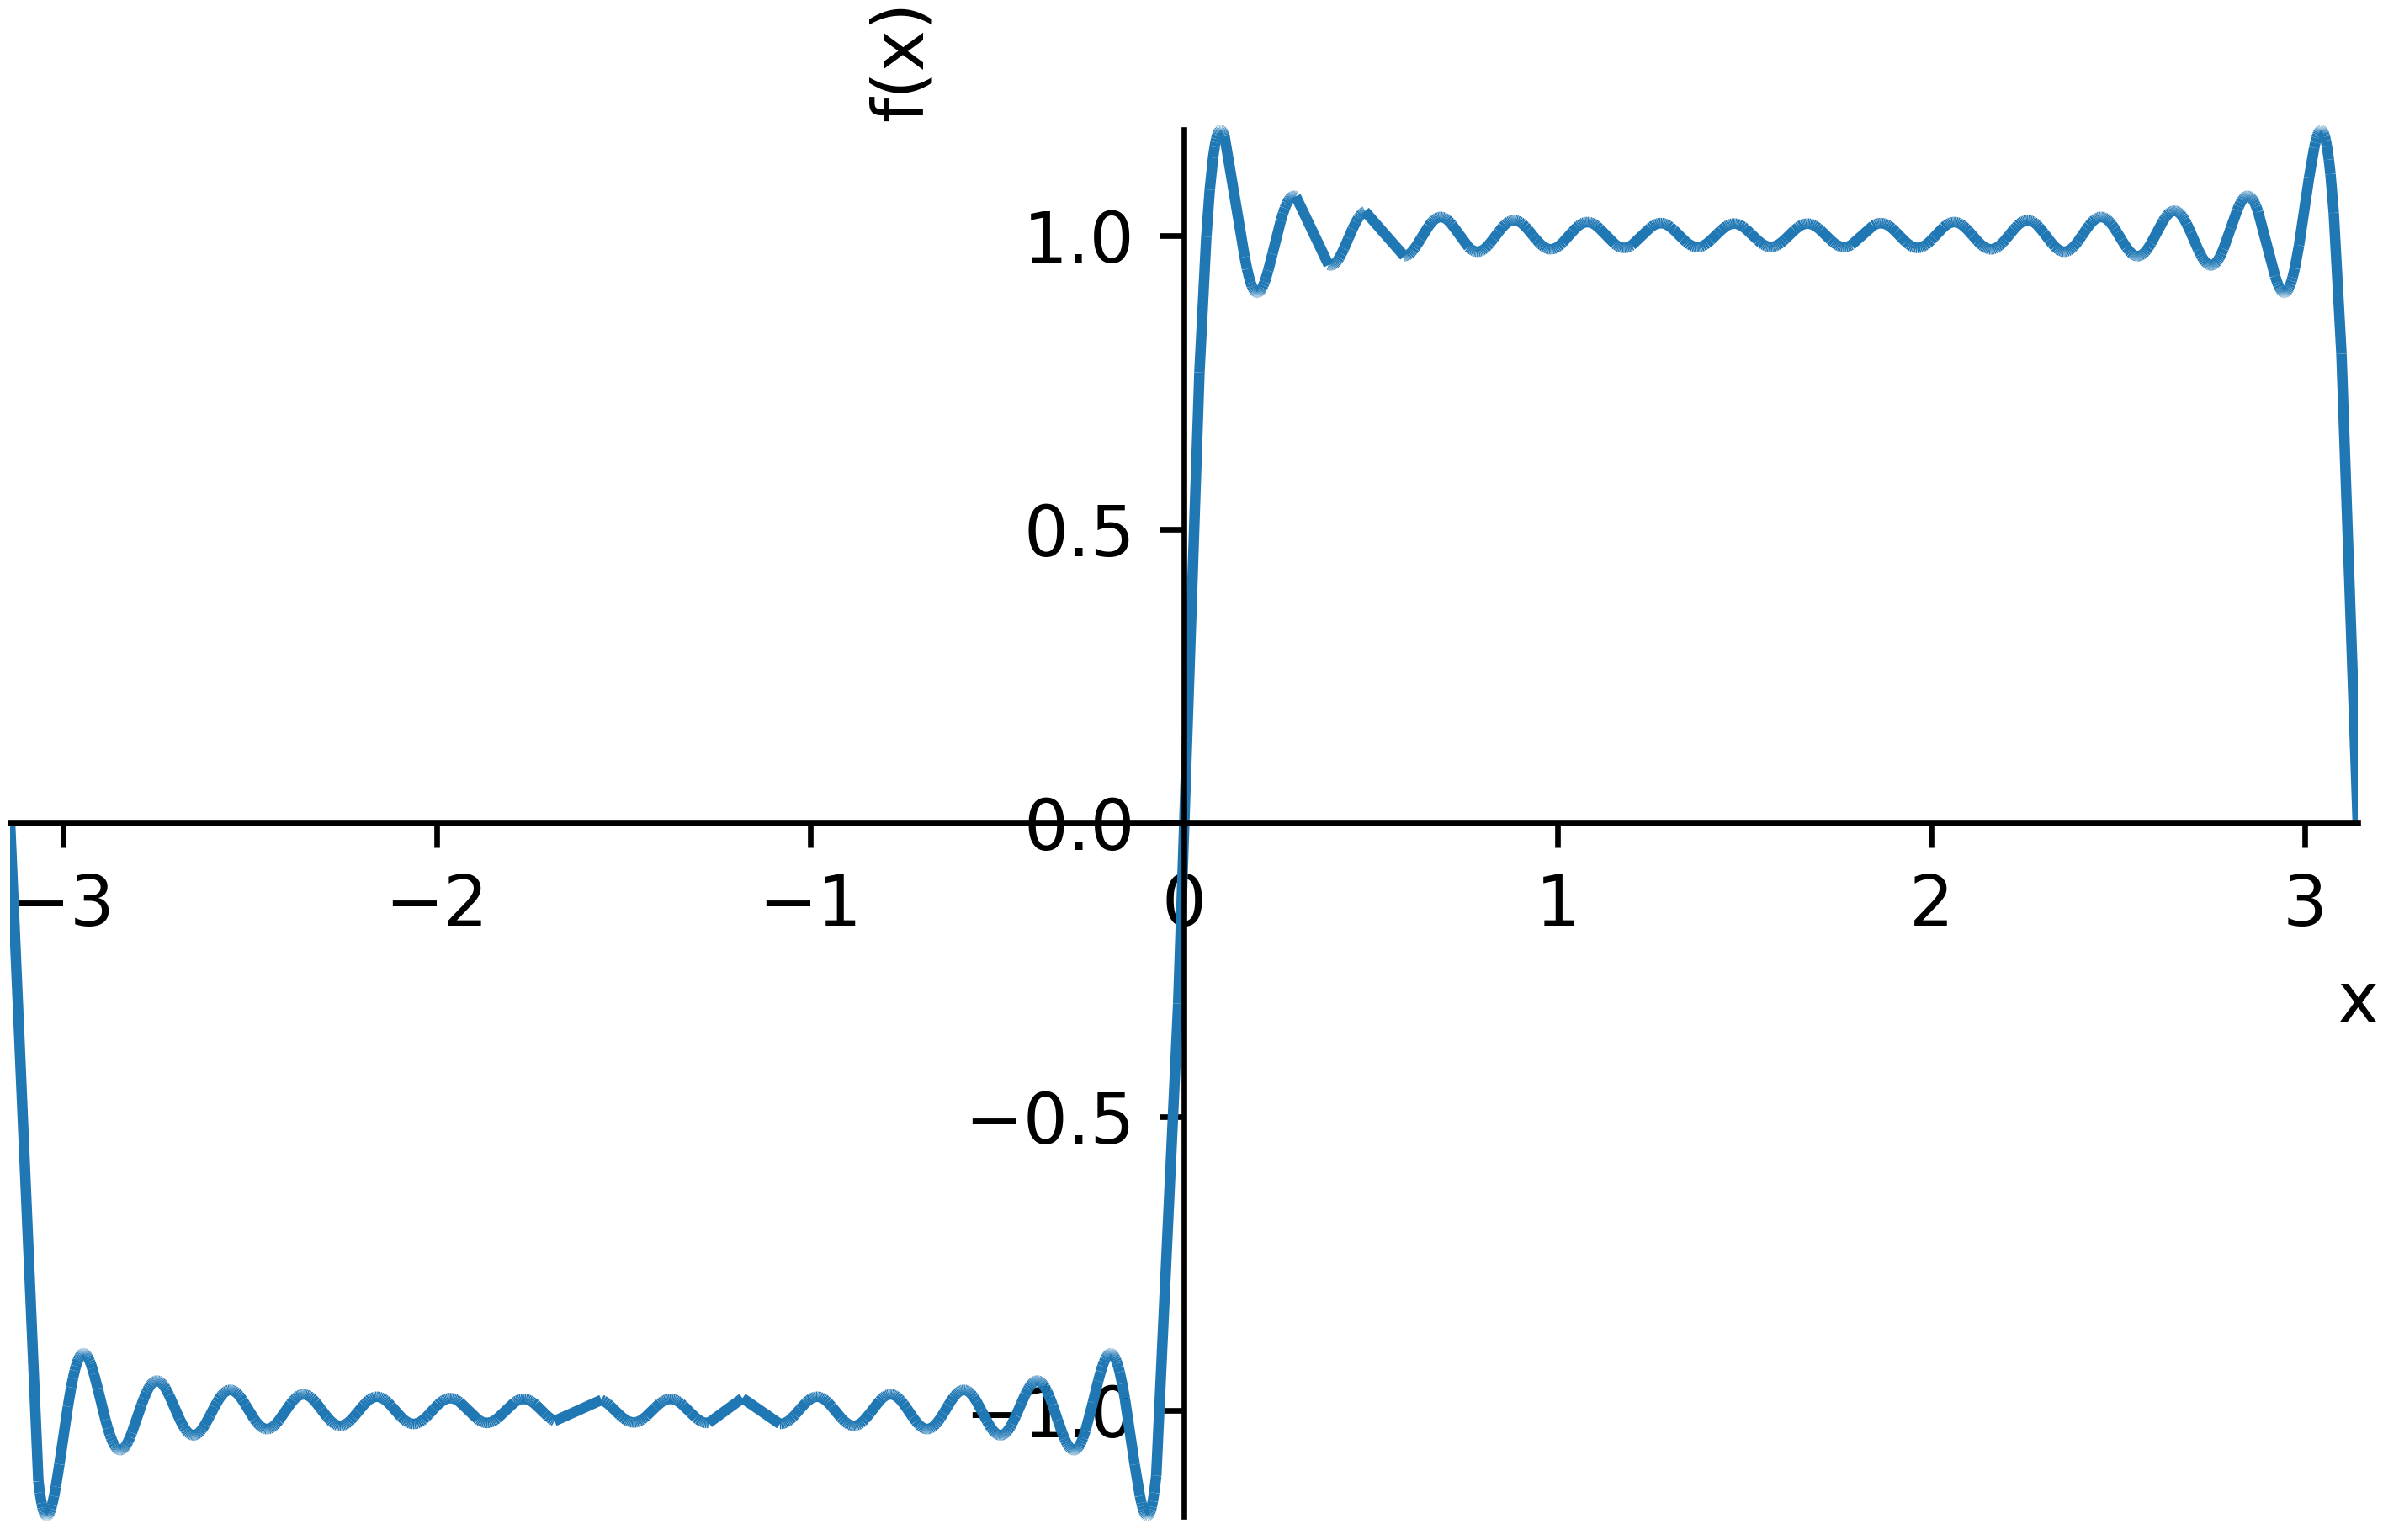
\includegraphics[height=5cm]{fourier.png}
\end{center}
\captionsetup{singlelinecheck=off}
\caption{Lo sviluppo di Fourier della funzione
che vale $1$ su $[0,\pi]$ e $-1$ su $[-\pi,0]$:
$
f_{61}(x)=
\frac{4\sin(x)}{\pi} + \frac{4\sin(3x)}{3\pi} + \frac{4\sin(5x)}{5\pi} + \frac{4\sin(7x)}{7\pi} + \frac{4\sin(9x)}{9\pi} + \frac{4\sin(11x)}{11\pi} + \frac{4\sin(13x)}{13\pi} + \frac{4\sin(15x)}{15\pi} + \frac{4\sin(17x)}{17\pi} + \frac{4\sin(19x)}{19\pi} + \frac{4\sin(21x)}{21\pi} + \frac{4\sin(23x)}{23\pi} + \frac{4\sin(25x)}{25\pi} + \frac{4\sin(27x)}{27\pi} + \frac{4\sin(29x)}{29\pi} + \frac{4\sin(31x)}{31\pi}
$.
Il codice python per generare il grafico
a pagina~\pageref{code:Fourier}
}
\label{fig:fourier}
\end{figure}

Risulta naturale chiedersi se quella che abbiamo introdotto è una
\emph{base hilbertiana} perché solo in tal caso gli sviluppi di Fourier
approssimano la funzione.
Per ottenere questo risultato dobbiamo assumere la validità del seguente
teorema, che sarebbe ora troppo lungo dimostrare.

\begin{theorem}[densità dei polinomi trigonometrici]
Per ogni funzione continua $f\in C^0([a,b])$
esiste una successione $g_k\in \H(a,b)$ di polinomi trigonometrici
(cioè combinazioni lineari finite del sistema $\{e_k\}$)
tale che $g_k$ converge uniformemente a $f$.

Detto in altri termini: l'insieme dei polinomi trigonometrici
è denso nello spazio $C^0([a,b])$ rispetto alla norma uniforme.
\end{theorem}

Osserviamo che la convergenza uniforme è più forte della convergenza
in $H(a,b)$ in quanto si ha, banalmente:
\[
  \Abs{f}_2^2 = \int_a^b f(x)^2\, dx
  \le \int_a^b \Abs{f}_\infty^2\, dx
  = (b-a) \Abs{f}_\infty^2.
\]
Dunque il teorema precedente garantisce che ogni funzione continua
in $\H(a,b)$ può essere approssimata, rispetto alla norma $\Abs{\cdot}_2$,
tramite polinomi trigonometrici. Il teorema seguente ci permette
di estendere questa proprietà a tutte le funzioni di $\H/(a,b)$.

\begin{theorem}[densità delle funzioni continue]
Data una qualunque $f\in H(a, b)$ per ogni $\eps>0$
esiste una funzione continua $g\colon [a,b]\to \RR$
tale che $\Abs{f-g}_2<\eps$.

Detto in altri termini: $C^0([a,b])$ è un sottospazio denso in $H(a,b)$
cioè un insieme la cui chiusura (nella topologia di $H(a,b)$) è tutto $H(a,b)$.
\end{theorem}
%
\begin{proof}
Se $f\in H(a,b)$ si ha,
per la disuguaglianza di Cauchy-Schwarz:
\[
  \int_a^b \abs{f(x)}\, dx
  \le \Abs{1}_2 \cdot \Abs{f}_2 = \sqrt{b-a}\cdot \Abs{f}_2 < +\infty.
\]
Dunque la funzione $f$ è assolutamente integrabile su $(a,b)$.
Se $f$ è limitata su $(a,b)$ possiamo pensare che $f$ sia definita su $[a,b]$
e l'integrale è un usuale integrale di Riemann (non improprio).
Per le condizioni di integrabilità sappiamo che per ogni $\eps>0$ è possibile
trovare una suddivisione $a=x_0 < x_1 < \dots < x_n =b$ su cui l'integrale
di $f$ differisce dagli integrali superiore e inferiore per meno di $\eps$.
Possiamo prendere come funzione $g$ una interpolazione lineare
cioè una funzione tale che si abbia $g(x_k) = f(x_k)$ sui punti della suddivisione
e che risulti lineare su ogni intervallino $[x_k,x_{k+1}]$. La funzione
$g$ così definita è compresa, su ogni intervallino, tra l'$\inf$ e il $\sup$
di $f$ e dunque si avrà:
\[
 \int_a^b \abs{f(x)-g(x)}\, dx < \eps.
\]
Visto però che $f$ è limitata sappiamo esistere $M>0$ per cui $\Abs{f}_\infty\le M$
e di conseguenza $\Abs{g}_\infty\le M$ e quindi $\Abs{f-g}_2\le 2M$.
Ma allora
\[
  \Abs{f-g}_2^2 = \int_a^b \abs{f(x)-g(x)}^2\, dx
  \le \int_a^b \Abs{f-g}_\infty \cdot \abs{f(x)-g(x)}\, dx
  \le 2M \eps.
\]
Abbiamo quindi mostrato che una funzione limitata e integrabile può essere
approssimata con funzioni continue.

Se la funzione è integrabile in senso improprio su $(a,b)$ ma non è limitata, per
definizione di integrale improprio per ogni $\eps>0$ possiamo trovare un intervallo
$[\alpha,\beta]\subset (a,b)$
per $f$ risulta limitata su $[\alpha,\beta$] e
l'integrale di $f$ su $(a,b)$ differisce dall'integrale di $f$ su $[\alpha,\beta]$
per meno di $\eps$. Ci possiamo quindi ricondurre al passo precedente
per trovare una funzione $g$ che approssima bene $f$ sull'intervallo $[\alpha,\beta]$.
Estendendo $g$ in modo costante su $(a,b)\setminus[\alpha,\beta]$ si troverà
una funzione che approssima bene $f$ su tutto $(a,b)$.
\end{proof}

Grazie ai due teoremi precedenti sappiamo che ogni $f\in \H(a,b)$ può essere
approssimata da polinomi trigonometrici $g_N\to f$
cioè da funzioni della forma:
\[
  g_N = \sum_{k=0}^{N} a_{k,N} e_k.
\]
Stiamo qui assumendo che il polinomio trigonometrico $g_N$ abbia ordine non superiore
ad $N$, ma questo si può sempre assumere, scartando
o ripetendo i termini della successione.

Se ora consideriamo gli sviluppi di Fourier:
\[
  f_N = \sum_{k=0}^N c_k e_k, \qquad c_k = \langle f,e_k\rangle
\]
ci ricordiamo che per ogni $k\le N$ risulta
\[
   \langle f-f_N, e_k \rangle
   = \sum{k=0}^N \enclose{\langle f,e_k\rangle - c_k} = 0
\]
e quindi
\[
  \langle f-f_N , g_N -f_N\rangle
  = \sum_{k=0}^N \langle f-f_N, (a_{k,N}-c_k) e_k \rangle
  = 0.
\]
Dunque, applicando il teorema di Pitagora,
\[
  \Abs{f-f_N}_2^2 = \Abs{f-g_N}_2^2 - \Abs{f_N-g_N}_2^2
  \le \Abs{f-g_N}_2^2 \to 0.
\]
Questo significa, dunque, che il sistema ortonormale che abbiamo introdotto
è una base hilbertiana e quindi che ogni funzione $f\in \H(a,b)$ si approssima
rispetto alla norma $\Abs{\cdot }_2$ con gli sviluppi di Fourier.

Ricordiamo che se $\Abs{f_N-f}_2 \to 0$ non è detto che si abbia la convergenza
puntuale $f_N(x)\to f(x)$ per ogni $x\in (a,b)$ in quanto il limite è unico
in $H(a,b)$ ma non in $\H(a,b)$ e dunque è possibile (e in effetti può succedere)
che il limite puntuale degli sviluppi di Fourier differisca, in alcuni punti,
dalla funzione che si sta approssimando.

Purtroppo lo spazio $H(a,b)$ non risulta essere
completo, come si può vedere nel seguente esempio.

\begin{example}[razionali ingrassati]
\label{ex:incompletezza_di_H}
Vogliamo mostrare che lo spazio $H(0,1)$ non è completo.
Sappiamo che l'insieme $[0,1]\cap \QQ$ è numerabile, quindi esiste una
successione $q_k$ che elenca tutti i numeri razionali nell'intervallo $[0,1]$.
Poniamo inoltre $r_k = \frac{1}{4\cdot 2^k}$ e consideriamo gli intervalli
$I_k = [q_k-r_k,q_k+r_k]$.
Prendiamo la successione di funzioni $f_n\colon [0,1]\to \RR$
definita da
\[
  f_n(x) =
  \begin{cases}
  1 &\text{se } x\in\displaystyle\bigcup_{k=1}^{n} I_k\\
  0 & \text{altrimenti}
  \end{cases}
\]
A differenza di quanto uno potrebbe pensare, queste funzioni $f_n$ non diventano
mai identicamente uguali ad $1$. Anzi, si può osservare che
\[
  \int_0^1 f_n(x)\, dx
  \le \sum_{k=1}^n \int_{q_k-r_k}^{q_k+r_k} 1\, dx
  = \sum_{k=1}^n \frac{1}{2\cdot 2^k}
  \le \frac{1}{2}\sum_{k=1}^{+\infty}\frac{1}{2^k} = \frac 1 2.
\]

Vogliamo ora mostrare che $f_k$ è una successione di Cauchy in $H(0,1)$ e
che però non converge in $H(0,1)$.

Per verificare che $f_n$ è una successione di Cauchy possiamo semplicemente
osservare che se $n\ge m$ risulta che $f_n$ e $f_m$ differiscono solamente
sugli intervalli $I_k$ con $k$ compreso tra $m$ ed $n$. Dunque:
\[
  \int_0^1 \abs{f_n - f_m}
  \le \sum_{k=m}^{+\infty} \int_{q_k-r_k}^{q_k+r_k} 1\,dx
  = \sum_{k=m}^{+\infty}\frac{1}{2\cdot 2^k} = \frac{1}{2^m}.
\]
Visto che $f_n$ e $f_m$ assumono solamente i valori $0$ e $1$ anche $\abs{f_n-f_m}$
assume solamente i valori $0$ e $1$ quindi $\abs{f_n-f_m}^2=\abs{f_n-f_m}$.
Abbiamo quindi verificato che per $n\ge m$ si ha:
\[
  \Abs{ f_n - f_m}_2 \le \sqrt{\frac{1}{2^m}}.
\]
E' dunque chiaro che comunque sia scelto $\eps>0$ possiamo scegliere $N$
tale che $1/2^N \le \eps^2$ da cui si ottiene che se $n,m\ge N$
allora $\Abs{ f_n-f_m}_2 \le \eps$. Cioè: $f_n$ è una successione di Cauchy.

Supponiamo ora, per assurdo, che esista $f\in H(0,1)$
tale che $\Abs{ f_n-f}_2 \to 0$.
Innanzitutto visto che ogni $f_k\le 1$ possiamo supporre che sia anche $f\le 1$
perché altrimenti potremmo prendere $g(x) = \min\{f(x),1\}$ e avremmo
chiaramente $\Abs{f_n - g}_2 \le \Abs{f_n -f}_2 \to 0$. In pratica stiamo dicendo
che modificando la funzione $f$ senza cambiarne l'integrale possiamo suppore
che $f(x)\le 1$ per ogni $x\in[0,1]$.

Fissato un intervallo $I_n$, per $k\to +\infty$ si ha:
\[
  0\le \int_{q_n-r_n}^{q_n+r_n}\abs{f_k(x)-f(x)}^2\, dx
  \le \int_0^1 \abs{f_k(x)-f(x)}^2\, dx = \Abs{ f_k -f}_2^2 \to 0.
\]
Ma ora se $k\ge n$ risulta che $f_k=1$ su $I_n$ e quindi il valore dell'integrale
precedente non dipende da $k$ e dovrà quindi essere identicamente nullo:
\[
  \int_{q_n-r_n}^{q_n+r_n} f(x) - 1 \, dx = 0
\]
e quindi possiamo affermare che $\sup f(I_n) = 1$ in quanto se fosse
$\sup f(I_n) = \lambda < 1$
l'integrale di $f(x)-1$ sarebbe negativo
sull'intervallo $I_n$.

Vogliamo ora dimostrare che su ogni intervallo $[a,b]\subset[0,1]$ si ha
$\sup f([a,b])=1$. Prendiamo $N$ abbastanza grande in modo che $r_N < (b-a)/3$.
Allora l'intervallo $[a+r_n, b-r_n]$ ha ampiezza $r_n$ e contiene infiniti
numeri razionali. Esistono quindi infiniti indici $n$ per cui $q_n$ sta in tale
intervallo. Tra questi infiniti certamente ce n'è uno con indice $n\ge N$
(perché i $q_n$ con $n< N$ sono in numero finito). Ma se $q_n \in [a+r_n,b-r_n]$
allora $I_n\subset[a,b]$ e quindi $\sup f([a,b])\ge \sup f(I_n) = 1$.

Questo significa che per ogni suddivisione di Riemann dell'intervallo $[0,1]$
risulta che il $\sup$ di $f$ sugli intervallini della suddivisione è $1$ e quindi
l'integrale superiore di $f$ è anch'esso $1$. Dunque, essendo $f$ integrabile,
\[
  \int_a^b f(x) = 1.
\]

Vogliamo ora concludere che questo è in contraddizione con la disuguaglianza
\[
  \int_a^b f_n(x) \le \frac 1 2
\]
che abbiamo osservato all'inizio.
Si ha infatti per la disuguaglianza di Cauchy-Schwarz
\begin{align*}
  \int_0^1 \abs{f(x)-f_n(x)}\, dx
  \le \Abs{f-f_n}_2\cdot \Abs{1}_2  \to 0
\end{align*}
e quindi, per il criterio di convergenza assoluta,
\[
  \int_0^1 (f(x) - f_n(x))\, dx \to 0.
\]
Ma abbiamo visto che
\[
  \int_0^1 (f(x) - f_n(x))\, dx
  = \int_0^1 f(x)\, dx - \int_0^1 f_n(x)\, dx
  \ge 1 - \frac 1 2 = \frac 1 2
\]
ottenendo quindi un assurdo.
\end{example}

Il fatto di avere trovato una base hilbertiana di $H(a,b)$ ci permette di
dire che ogni funzione in $H(a,b)$ può essere rappresentata dalle sue
coordinate $c_k$ in modo che valga l'uguaglianza di Bessel:
\[
  \Abs{f}_2 = \sqrt{\sum_{k=0}^{+\infty} c_k^2}.
\]
Abbiamo in effetti definito una corrispondenza:
\[
  \phi \colon H(a,b) \to \ell^2,
  \qquad
  \ell^2=\{c\in \NN^\RR \colon \sum_{k=0}^{+\infty} c_k^2<+\infty\}
\]
definita da
\[
  c_k = \phi(f) = \langle f, e_k\rangle.
\]
Chiaramente tale $\phi$ è lineare. Visto che $e_k$ è una base hilbertiana
è facile verificare che $\phi$ è anche iniettivo. Se su $\ell^2$
definiamo il prodotto scalare e la norma corrispondente:
\[
  \langle x,y\rangle = \sum_{k=0}^{+\infty} x_k y_k, \qquad
  \abs{x}_2 = \sqrt{\sum_{k=0}^{+\infty}} x_k^2
\]
l'uguaglianza di Bessel ci dice che $\phi$ mantiene la norma e quindi
la struttura di spazio euclideo. Si potrebbe dimostrare che $\ell^2$
è completo e questo significa che $\phi$ non è suriettiva in quanto
la successione $f_n$
considerata nell'esempio~\ref{ex:incompletezza_di_H}
è di Cauchy in $H(a,b)$, dunque $\phi(f_n)$ è di Cauchy in $\ell^2$
e dunque converge in $\ell^2$. Il limite $c$ della successione $\phi(f_n)$
rappresenta una successione di coefficienti di Fourier che non possono
essere ottenuti da nessuna funzione $f\in H(a,b)$.

\section{divagazione sui frattali autosimili}

\begin{definition}
Siano $A$ e $B$ sottoinsiemi non vuoti di $\RR^n$.
Definiamo la \emph{distanza di Hausdorff}
\mynote{distanza di Hausdorff}
\index{distanza!di Hausdorff}
tra $A$ e $B$ come:
\[
  d_{\H}(A,B) = \max\big\{\sup_{a\in A}\inf_{b\in B} \abs{a-b}, \sup_{b\in B} \inf_{a\in A} \abs{a-b}\big\}.
\]

Definiamo
\[
 \K(\RR^n) = \{A \subset \RR^n \colon \text{$A$ chiuso, limitato, non vuoto}\}.
\]
\end{definition}

\begin{theorem}[caratterizzazione della distanza di Hausdorff]
Se $A$ e $B$ sono compatti di $\RR^n$ (cioè chiusi e limitati) allora
per ogni $r \in \RR$
si ha
\[
  d_\H(A,B) \le r
\]
se e solo se valgono entrambe le seguenti proprietà:
\begin{enumerate}
\item per ogni $a\in A$ esiste $b\in B$ tale che $\abs{a-b}\le r$;
\item per ogni $b\in B$ esiste $a\in A$ tale che $\abs{a-b}\le r$.
\end{enumerate}
\end{theorem}
%
\begin{proof}
Per ogni compatto non vuoto $A$ e per ogni $x\in \RR^n$ definiamo
la distanza tra il punto $x$ e l'insieme $A$ come:
\[
  d(x,A) = \min_{a\in A} \abs{x-a}.
\]
Il minimo esiste in quanto $A$ è compatto e $a\mapsto d(x,a)$ è una funzione continua. Fissato $A$ la funzione $x\mapsto d(x,A)$ è anch'essa continua, anzi è $1$-lipschitziana. Infatti se $x'\in \RR^n$ esiste $a'\in A$ tale che $d(x',A) = d(x',a')$ e dunque
\[
  d(x,A) = \min_{x\in A} \abs{x-a} \le \abs{x-a'} \le \abs{x-x'} + \abs{x'- a'}
   = \abs{x-x'} + d(x',A)
\]
da cui $d(x,A) - d(x',A)\le \abs{x-x'}$.
Scambiando $x$ e $x'$ si ottiene anche la disuguaglianza inversa da cui la $1$-lipschitzianità di $d(x,A)$. Dunque sui compatti la funzione $d(x,A)$ assume sempre massimo e si ha:
\[
d_\H(A,B) = \max\{\max_{a_\in A} d(a,B), \max_{b\in B} d(b,A)\}.
\]

In particolare se $d_\H(A,B) \le r$ per ogni $a\in A$ si deve avere $d(a,B) \le r$ e per ogni $b\in B$ si deve avere $d(b,A) \le r$. Ma allora valgono le due proprietà dell'enunciato.

Viceversa se vale la proprietà 1.\ allora $d(a,B)\le r$ e se vale la 2.\ $d(b,A)\le r$ e di conseguenza $D_\H(A,B) \le r$.
\end{proof}

\begin{theorem}[distanza di Hausdorff]
La distanza di Hausdorff $d_\H$ è una distanza su $\K(\RR^n)$ e lo spazio metrico $\K(\RR^n)$ è completo.
\end{theorem}
%
\begin{proof}
Chiaramente se $A,B$ sono non vuoti si ha $d_\H(A,B) \ge 0$.
Inoltre, in base alla caratterizzazione del teorema precedente è facile osservare che $d_\H(A,B) < +\infty$.

Se $d_\H(A,B) = 0$ significa che per ogni $a\in A$ esiste $b\in B$ tale che $\abs{a-b}=0$. Cioè $b=a$. Dunque $A\subset B$. Scambiando i ruoli di $A$ e $B$ si ottiene anche $B\subset A$ da cui $A=B$.

Che sia $d_\H(A,B) = d_\H(B,A)$ è ovvio in quanto la definizione è simmetrica in $A$ e $B$.

Verifichiamo ora la disuguaglianza triangolare. Siano $A,B,C$ tre compatti non vuoti. Per ogni $a\in A$ esiste $b\in B$ tale che $\abs{a-b} \le d_\H(A,B)$ e per tale $b \in B$ esiste un $c\in C$ tale che $\abs{b-c} \le d_\H(B,C)$. Dunque per ogni $a\in A$ esiste un $c\in C$ tale che
\[
  \abs{a-c} \le \abs{a-b} + \abs{b-c} \le d_\H(A,B) + d_\H(B,C).
\]
Scambiando i ruoli di $A$ e $C$ si ottiene anche la condizione simmetrica e dunque, per la caratterizzazione della distanza di Hausdorff si ottiene la disuguaglianza triangolare:
\[
  d_\H(A,C) \le d_\H(A,B) + d_\H(B,C).
\]

Abbiamo quindi verificato che $d_\H$ è una distanza su $\K(\RR^n)$. Verifichiamo ora che $\K(\RR^n)$ è completo.

Sia $A_k\in\K(\RR^n)$ una successione di Cauchy.
Senza perdita di generalità possiamo supporre che
\[
  d_\H(A_k,A_{k+1}) \le \frac{1}{2^k}.
\]
Infatti essendo $A_k$ di Cauchy è possibile trovarne una sottosuccessione con tale proprietà, e se poi dimostriamo che la sottosuccessione converge allora l'intera successione, essendo di Cauchy, deve convergere.

Consideriamo come candidato limite l'insieme di tutti i possibili limiti di punti degli insiemi $A_k$:
\[
  A = \{x\in \RR^n
  \colon \exists x_k \in A_k\colon x_k \to x\}.
\]

Per prima cosa vogliamo verificare che $A$ non è vuoto. Scelto un punto qualunque $a_0 \in A_0$ esiste $a_1 \in A_1$ tale che $\abs{a_0 - a_1} = d_\H(A_0,A_1)$. Iterando otteniamo una successione di punti $a_k \in A_k$ tale che $\abs{a_k - a_{k+1}} \le d_\H(A_k,A_{k+1}) \le 1/2^k$.
Dunque $a_k$ è una successione di Cauchy in $\RR^n$ ed essendo $\RR^n$ completo dovrà convergere ad un punto $a$ che quindi è un punto di $A$.

Avendo assunto $d_\H(A_k, A_{k+1}) < 1/2^k$ si ottiene (sommando la serie geometrica):
\[
 d_\H(A_k, A_n) \le \sum_{j=k}^{n-1} d_\H(A_j, A_{j+1}) \le \frac{2}{2^k}\qquad \text{se $n>k$}.
\]
Questo ci permette di dimostrare che per ogni $a\in A$ e per ogni $k\in \NN$ esiste $a_k \in A_k$ tale che
$\abs{a - a_k}\le 4/2^k$. Infatti se a distanza $4/2^k$ non ci fossero punti di $A_k$ allora a distanza $2/2^k$ non ci potrebbero essere punti di $A_n$ per nessun $n>k$ in quanto visto che $d_\H(A_k,A_n) \le 2/2^k$ se ci fosse un punto di $A_n$ a distanza inferiore a $2/2^k$ ci dovrebbe anche essere un punto di $A_k$ a distanza inferiore a $4/2^k$. Ma questo è impossibile perché per come è definito $A$ deve esistere $x_n \in A_n$ tale che $x_n \to a$. Abbiamo quindi mostrato che
\[
  \sup_{a\in A} \inf_{b\in A_k} \abs{a-b} \le 4/2^k \to 0.
\]

Viceversa ci proponiamo di mostrare che per ogni $p \in A_k$ esiste $a \in A$ tale che $\abs{p-a} < 2/2^k$.
Visto che $d_\H(A_{j+1},A_j) \le 1/2^j$
possiamo infatti costruire a partire da $a_k=p \in A_k$
una successione $a_j \in A_j$ con $j > k$, tale che $d(a_{j+1},a_j) \le 1/2^j$. Tale successione è di Cauchy
quindi converge: $a_j \to a$
e il suo limite $a$ è quindi un punto di $A$ e si ha
\[
  \abs{a-p} \le \sum_{j=k}^\infty \abs{a_j - a_{j+1}}
    \le \sum_{j=k}^\infty \frac{1}{2^j} \le \frac{2}{2^k}.
\]
Abbiamo quindi dimostrato che
\[
  \sup_{b\in a_k} \inf_{a\in A} \abs{a-b} \le 2/2^k \to 0
\]
e quindi $d_\H(A_k,A)\to 0$.

Ci rimane solo da mostrare che $A$ è un insieme chiuso.
Presa una successione di punti $x_k\in A$ convergente $x_k\to x$, dobbiamo mostrare che $x\in A$. Per ogni $x_k\in A$ per quanto già detto sappiamo esistere $a_k \in A_k$ tale che $\abs{a_k-x_k}\le 4/2^k$. Ma allora $\abs{a_k-a} \le 4/2^k + \abs{x_k-a} \to 0$ e quindi $a_k\to a$ da cui $a\in A$.
 \end{proof}

\begin{theorem}[frattali autosimilari]
Siano $\phi_1, \dots, \phi_N \colon \RR^n \to \RR^n$ contrazioni (cioè funzioni lipschitziane con costante di lipschitz inferiore ad $1$).
Allora
esiste un unico insieme $C\subset \RR^n$ chiuso e limitato tale che
\[
  C = \bigcup_{k=1}^N \phi_k(C).
\]
\end{theorem}
%
\begin{proof}
Basterà dimostrare che la funzione $T\colon \K(\RR^n)\to \K(\RR^n)$ definita da
\[
  T(A) = \bigcup_{k=1}^N \phi_k(C)
\]
è una contrazione: dopodiché sapendo che $\K(\RR^n)$ è completo il risultato è conseguenza diretta del teorema di punto fisso di Banach-Caccioppoli.

Ogni $\phi_k$ per ipotesi è una contrazione, cioè
per ogni $a,b\in X$
\[
  \abs{\phi_k(a)-\phi_k(b)} \le L_k \abs{a-b}
\]
con $L_k< 1$. Posto $L=\max \{L_1, \dots, L_N\} < 1$ vogliamo dimostrare che $T$ è $L$-lipschitziana (e dunque una contrazione). Siano $A,B \in \K(\RR^n)$ e sia $d = d_\H(A,B)$. Preso $a' \in T(A)$ dovrà esistere $k$ tale che $a' \in \phi_k(A)$. Cioè $a'= \phi_k(a)$ con $a\in A$. Ma allora esiste $b\in B$ con $\abs{a-b}\le d_\H(A,B) = d$ e quindi $b'=\phi_k(b) \in T(B)$ e $\abs{a'-b'} = \abs{\phi_k(a)-\phi_k(b)} \le L \abs{a-b} \le L \cdot d$. Dunque abbiamo mostrato che
\[
  \sup_{a' \in T(A)} \inf_{b'\in T(B)} \abs{a'-b'} \le L d_\H(A,B).
\]
La stessa disuguaglianza rimane valida con $A$ e $B$ scambiati, ottenendo quindi:
\[
  d_\H(T(A),T(B)) \le L\cdot d_\H(A,B).
\]
\end{proof}

\begin{example}[insieme di Cantor]
Si prendano $\phi, \psi\colon \RR \to \RR$ definite da
\[
  \phi(x) = \frac{x}{3}, \qquad
  \psi(x) = \frac{2+x}{3}.
\]
Chiaramente $\phi$ e $\psi$ sono $1/3$-lipschitziane e dunque, per il teorema precedente, esiste un unico insieme $C$ chiuso e limitato in $\RR$ tale che
\[
  C = \frac{C}{3} \cup \frac{C+2}{3}.
\]
Tale insieme si chiama \myemph{insieme di Cantor}.

L'insieme di Cantor è un frattale autosimile in quanto si ottiene come l'unione di due copie riscalate di sé stesso.

E' facile mostrare che $C\subset [0,1]$ in quanto $T$ manda sottoinsiemi di $[0,1]$ in sottoinsiemi di $[0,1]$.
Ogni $x\in [0,1]$ può essere rappresentato in base $3$ con una sequenza di cifre ternarie: $0,1,2$. La funzione $\phi(x)$ aggiunge uno $0$ in cima alla sequenza di cifre, mentre la funzione $\psi(x)$ aggiunge un $2$ in cima alla sequenza.
Vogliamo mostrare che $C$ è l'insieme di tutti i numeri in $[0,1]$ che possono essere scritti in base $3$ utilizzando solamente le cifre $0$ e $2$. Osserviamo innanzitutto che $C$ è chiuso: il suo complementare in $[0,1]$ è formato da tutti i numeri che in base $3$ si devono scrivere utilizzando almeno una cifra $1$. Ma se c'è una cifra $1$ possono modificare tutte le cifre successive rimanendo nel complementare di $C$: dunque il complementare di $C$ è aperto. Si osservi che gli unici numeri che hanno una doppia rappresentazione in base $3$ sono quelli che terminano con una sequenza infinita di $2$,
\end{example}

\begin{figure}
\centering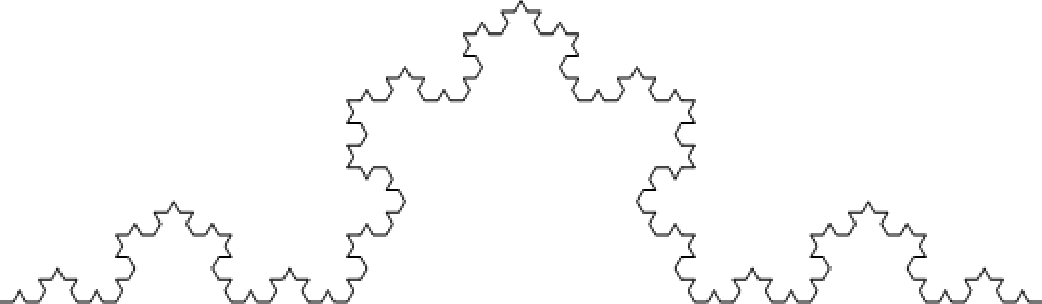
\includegraphics[width=1.0\textwidth]{koch_picture}
\caption{
Chiamato $K_0 \in \RR^2$ il segmento $[0,1]\times \{0\}$,
in figura è rappresentata
la quarta iterata $K_4 = T^4(K_0)$ della contrazione che definisce la curva di K{\"o}ch.
A pagina~\pageref{code:Koch} il codice per generare la figura in copertina.
\index{curva di K{\"o}ch}
}
\label{fig:koch}
\end{figure}

\begin{example}[curva di K{\"o}ch]
Sia $R_\theta\colon \RR^2 \to \RR^2$ la rotazione di $\RR^2$ con centro l'origine di $\theta$ radianti in senso antiorario.
Sia $\alpha = \pi/3$, $p=(1,0)$ e
siano $\phi_1, \phi_2, \phi_3, \phi_4 \colon \RR^2 \to \RR^2$
le funzioni definite da:
\begin{align*}
\phi_1(v) = \frac{v}{3}, \qquad
\phi_2(v) = R_{\alpha}\frac{v}{3} + \phi_1(p), \\
\phi_3(v) = R_{-\alpha}\frac{v}{3} + \phi_2(p), \qquad
\phi_4(v) = \frac{v}{3} + \phi_3(p).
\end{align*}
Allora esiste un unico insieme chiuso $K\subset \RR^2$ tale che
\[
  K = \phi_1(K) \cup \phi_2(K) \cup \phi_3(K) \cup \phi_4(K).
\]
L'insieme $K$ si chiama \myemph{curva di K{\"o}ch}. E' un frattale autosimile in quanto è composto da quattro copie riscalate di se stesso.
\end{example}


\chapter{successioni ricorsive}
\label{ch:successioni_ricorsive}

In questo capitolo prenderemo in considerazione le successioni $a_n$
definite \emph{per ricorrenza} o \emph{ricorsivamente} dalle condizioni:
\index{successioni!ricorsive}
\index{successioni!definite per ricorrenza}
\index{ricorsione}
\begin{equation}\label{eq1}
\begin{cases}
  a_1 = \alpha,\\
  a_{n+1} = f(a_n)
\end{cases}
\end{equation}

Fissato il termine iniziale $\alpha$ e la legge di ricorrenza $f$,
c'è una unica successione che soddisfa \eqref{eq1} e i suoi termini
sono:
\begin{align*}
a_1 & =\alpha,\\
a_2 &= f(a_1)=f(\alpha),\\
a_3 &= f(a_2)=f(f(\alpha)),\\
a_4 &= f(a_3)=f(f(f(\alpha))),\\
\vdots
\end{align*}

Il valore di $a_n$ potrebbe rappresentare lo stato di un sistema che
si evolve a partire da uno stato iniziale $a_1$ tramite la
funzione $f$ che rappresenta il cambiamento di stato.
Il numero naturale $n$ potrebbe quindi rappresentare un passo temporale.
In tal senso \eqref{eq1} si chiama anche \myemph{sistema!dinamico!discreto}.

L'equazione $a_{n+1} = f(a_n)$ viene chiamata una \emph{equazione
  autonoma del primo ordine}. Osserviamo infatti
che ci sono altre tipologie di equazioni che però
non considereremo in queste note. Ad esempio quando vogliamo definire
il fattoriale: $a_n = n!$ diamo le condizioni:
\[
\begin{cases}
  a_1 = 1\\
  a_{n+1} = (n+1) \cdot a_n
\end{cases}
\]
ma l'equazione $a_{n+1} = (n+1) \cdot a_n$ è della forma $a_{n+1} =
f(n, a_n)$ e si dice essere \emph{non autonoma} perché la funzione di
ricorrenza $f$ dipende esplicitamente da $n$ oltre che dal termine
precedente $a_n$.

Si potrebbero anche considerare equazioni di ordine maggiore del
primo. Ad esempio la successione di \emph{Fibonacci}
\mymargin{Fibonacci}
\index{Fibonacci!successione di}
\index{successione!di Fibonacci}
$F_n$ è definita da
\begin{equation}\label{eq:Fibonacci}
\begin{cases}
  F_1 = 1 \\
  F_2 = 1 \\
  F_{n+2} = F_{n+1} + F_n
\end{cases}
\end{equation}
che è una relazione del secondo ordine in quanto ogni termine può
essere definito utilizzando i valori dei \emph{due} termini precedenti.
Se l'equazione è lineare, come in questo caso, si possono trovare delle
formule esplicite per scrivere l'$n$-esimo termine della successione.
Lo faremo nella sezione~\ref{sec:ricorrenza_lineare}

Si potrebbero anche considerare i sistemi di equazioni ricorsive.
Ad esempio se $f$ fosse una funzione complessa $f\colon \CC \to \CC$
$f(x+iy) = f_1(x,y) + i f_2(x,y)$ con $f_1,f_2 \colon \RR\to\RR$
si potrebbe scrivere $a_n = x_n + i y_n$ con $x_n, y_n \in \RR$
l'equazione ricorsiva $a_{n+1} = f(a_n)$
diventerebbe un sistema di due equazioni:
\[
  \begin{cases}
    x_{n+1} = f_1(x_n, y_n)\\
    y_{n+1} = f_2(x_n, y_n).
  \end{cases}
\]
Lo studio dei sistemi va oltre gli scopi di questo capitolo,
ma accenneremo solamente ad un esempio nella sezione~\ref{sec:mandelbrot}.

\section{equazioni ricorsive autonome del primo ordine}

\begin{exercise}[algoritmo di Erone]\label{ex_Erone}
\index{Erone!algoritmo di}
\index{algoritmo!di Erone}
\index{algoritmo!calcolo della radice $n$-esima}
\index{radice $n$-esima!algoritmo di Erone}
  Fissato un numero reale $p>1$ consideriamo la successione definita
  per
ricorrenza da
\[
\begin{cases}
  a_1 = p\\
  a_{n+1} = \frac{a_n + p/a_n}{2}.
\end{cases}
\]
Si dimostri che $a_n \to \sqrt p$.
\end{exercise}
Osserviamo, ad esempio, che per $p=2$ i
primi termini della successione sono:
\begin{align*}
a_1 &= 2, \\
a_2 &= \frac{2+2/2}{2} = 3/2 = 1.5, \\
a_3 &= \frac{3/2 + 2/(3/2)}{2} = 17/12 \approx 1.4166666, \\
a_4 &= \frac{17/12 + 2/(17/12)}{2} = 577 / 408 \approx 1.4142157,\\
\vdots
\end{align*}
che effettivamente \emph{sembrano} avvicinarsi molto al numero
\[
\sqrt 2\approx 1.4142135.
\]

\begin{proof}
\emph{Passo 1.} Dimostriamo per induzione che $a_n>0$ per ogni $n\in \NN$.
Infatti per $n=1$ osserviamo che $a_1=p>0$ mentre se supponiamo che
$a_n>0$ otteniamo che $a_{n+1} = (a_n + p/a_n)/2$ è positivo in quanto
è la metà della somma di due quantità positive. Quindi, applicando il
principio di induzione, possiamo concludere che $a_n>0$ per ogni $n$.

Abbiamo in effetti identificato un insieme $A=\ENCLOSE{x\colon x>0} = (0,
+\infty)$ tale che la funzione $f(x) = \frac{x + p/x}{2}$ è definita
su $A$ e, contemporaneamente, ha valori in $A$.
Quindi questo passaggio è fondamentale anche solo per
garantire che la successione $a_n$ sia ben definita.

\emph{Passo 2.} Dimostriamo che la successione $a_n$ è decrescente.
Per fare questo osserviamo che essere decrescente significa:
$ a_{n+1} \le a_n$
e cioé
\[
\frac{a_n + p/a_n}{2} \le a_n
\]
ovvero (moltiplicando ambo i lati per $a_n>0$)
\[
a_n^2 + p \le 2 a_n^2
\]
che è equivalente a $a_n^2 - p \ge 0$. E, in effetti, questa
disuguaglianza è sempre vera in quanto per $n=1$ si riduce a $a_1^2 - p
= p^2 - p \ge 0$ che è soddisfatta nel caso $p>1$. Mentre
\begin{align*}
a_{n+1}^2 - p & = \left(\frac{a_n+p/a_n}{2}\right)^2 - p
= \frac{a_n^4 + 2 p a_n^2 + p^2 - 4 p a_n^2}{4 a_n^2} \\
& = \frac{a_n^2 - 2 p a_n^2 + p^2}{4 a_n^2}
 = \frac{\left(a_n^2 - p\right)^2}{4a_n^2} \ge 0.
\end{align*}
Dunque $a_{n+1}^2 \ge p$ per ogni $n\in \NN$ e di conseguenza $a_n$ è
decrescente e inoltre $a_n > \sqrt p$.

\emph{Passo 3.}
Visto che $a_n$ è una successione decrescente
per il teorema sulle successioni monotòne possiamo
affermare che $a_n$ ammette limite, e cioé: $a_n \to \ell$ con $\ell
\in [-\infty, +\infty]$. Possiamo immediatamente escludere
$\ell=+\infty$ in quanto la successione è decrescente, e possiamo
anche escludere $\ell<\sqrt{p}$ in quanto sappiamo che $a_n > \sqrt{p}$ e quindi
(per il teorema della permanenza del segno) $\ell \ge \sqrt p$.
Inoltre
\[
  a_{n+1} = \frac{a_n + p/a_n}{2} \to \frac{\ell + p/\ell}{2}.
\]
Ma sappiamo che se $a_n\to \ell$ anche $a_{n+1}\to \ell$ (visto che
$a_{n+1}$ è una sottosuccessione di $a_n$) e quindi (per l'unicità del
limite)
\begin{equation}\label{ex_1_fixed}
  \ell = \frac{\ell + p/\ell}{2}
\end{equation}
da cui si ricava $\ell^2 = p$ ovvero (essendo $\ell\ge 0$) concludiamo
$a_n \to \ell =
\sqrt p$.
\end{proof}

Cominciamo ora a definire una terminologia e a fissare alcuni
risultati generali che ci serviranno per trovare alcune proprietà
delle successioni definite da~ \eqref{eq1}.

\begin{definition}[punto fisso]
\mymark{**}
  Diremo che $x$ è un \myemph{punto!fisso}
  per la funzione $f$ se vale
  \[
    f(x) = x.
  \]
\end{definition}
Osserviamo che se $\alpha$ è un punto fisso per $f$ la successione costante
$a_n=\alpha$ soddisfa l'equazione $a_{n+1} = f(a_n)$. Inoltre se
$a_{n+1} = f(a_n)$, se $a_n$ converge ad un limite $\ell$ e se
$\lim_{x\to \ell} f(x) = f(\ell)$ (diremo: $f$ è continua in $\ell$) allora
\[
a_{n+1} = f(a_n) \to f(\ell)
\]
ma visto che $a_{n+1}$ ha lo stesso limite di $a_n$ si trova che
$f(\ell)=\ell$ ovvero il limite della successione è un punto fisso.

Nell'esercizio precedente la funzione $f(x) = (x+p/x)/2$ ha come punti
fissi $\sqrt{p}$ e $-\sqrt{p}$ e l'equazione~\eqref{ex_1_fixed} non è
altro che $f(x)=x$. E in effetti abbiamo mostrato che la successione
$a_n$ converge proprio ad un punto fisso.

\begin{definition}[insieme invariante]
\mymark{**}
  Un insieme $A$ si dice essere \emph{invariante}
  \mynote{insieme invariante}
  per $f$ se
  $f(A)\subseteq A$.
\end{definition}

Osserviamo che se $A$ è un insieme invariante e $a_1\in A$ allora la
successione definita da $a_{n+1}=f(a_n)$ assume sempre valori in $A$.

Nell'esercizio~\ref{ex_Erone} abbiamo dimostrato che gli insiemi
$(0,+\infty)$ e $(\sqrt{p},+\infty)$ sono invarianti.

\begin{theorem}\label{th_1}
\mymark{*}
  Sia $A\subset \RR$ un insieme invariante per $f$ e sia $a_n$ una
  successione con $a_1 \in A$ e $a_{n+1}=f(a_n)$.

  Se per ogni $x\in A$
  vale $f(x) \ge x$
  \mynote{$f(x)\ge x$}
  allora la successione $a_n$ è crescente.

  Se per ogni $x\in A$ vale $f(x) \le x$
  \mynote{$f(x)\le x$}
  allora la successione $a_n$ è decrescente.
\end{theorem}
\begin{proof}
\mymark{*}
  In effetti se $f(x) \ge x$ si ha per ogni $n\in \NN$
  \[
  a_{n+1} = f(a_n) \ge a_n
  \]
e quindi la successione $a_n$ è crescente. Mentre se $f(x) \le x$ si ha
  \[
  a_{n+1} = f(a_n) \le a_n
  \]
e la successione è decrescente.
\end{proof}

\begin{exercise}
Al variare di $\alpha \in \RR$
determinare il limite della successione $a_n$ definita per ricorrenza dalle
equazioni:
\[
\begin{cases}
 a_1 = \alpha \\
 a_{n+1} = a_n - a_n^2.
\end{cases}
\]
\end{exercise}

\begin{theorem}
\mymark{**}
  Sia $A\subset \RR$ un insieme invariante per $f$ e sia $a_n$ una successione
  con $a_1\in A$ e $a_{n+1} = f(a_n)$. Se $f$ è crescente
  \mynote{$f$ crescente}
  su $A$ allora $a_n$
  è monotòna.
\end{theorem}
\begin{proof}
\mymark{**}
  Osserviamo che se $f$ è crescente allora
  \begin{align*}
    a_{n+1} \ge a_n \Rightarrow f(a_{n+1}) \ge f(a_n) \Rightarrow
    a_{n+2} \ge a_{n+1}\\
    a_{n+1} \le a_n \Rightarrow f(a_{n+1}) \le f(a_n) \Rightarrow a_{n+2} \le a_{n+1}.
  \end{align*}
  Dunque se per i primi due termini si ha $a_2 \ge a_1$ allora, per
  induzione, si ha $a_{n+1} \ge a_n$ per ogni $n$ e quindi la
  successione è crescente. Se invece $a_2 \le a_1$ si dimostra per
  induzione che $a_{n+1} \le a_n$ per ogni $n$ e quindi la successione
  è decrescente.
\end{proof}

\begin{theorem}\label{th_decr}
\mymark{**}
  Sia $A\subset \RR$ un insieme invariante per $f$ e sia $a_n$ una successione
  con $a_1\in A$ e $a_{n+1} = f(a_n)$. Se $f$ è decrescente
  \mynote{$f$ decrescente}
  su $A$
  allora le due successioni $a_{2n}$ (termini di indice pari) e
  $a_{2n+1}$ (termini di indice dispari) sono monotòne.
\end{theorem}
\begin{proof}
\mymark{**}
  Osserviamo che
  \begin{align*}
    a_{2n+2} &= f(a_{2n+1}) = f(f(a_{2n})) = (f\circ f)(a_{2n})\\
    a_{2n+3} &= f(a_{2n+2}) = f(f(a_{2n+1})) = (f\circ f)(a_{2n+1})
  \end{align*}
cioé le sottosuccessioni dei termini di indice pari e di indice
dispari soddisfano una relazione di ricorrenza tramite la funzione
$f\circ f$ (invece che $f$).

Osserviamo anche che se $f$ è decrescente allora $f\circ f$ è
crescente. Infatti:
\[
x \le y \Rightarrow f(x) \ge f(y) \Rightarrow f(f(x)) \le f(f(y)).
\]

Dunque possiamo applicare il teorema precedente e ottenere che le due
sottosuccessioni sono entrambe monotòne.
\end{proof}

Utilizziamo la terminologia e i risultati precedenti nei seguenti
esercizi.

\begin{exercise}[Fibonacci]\label{ex_fibonacci}
\index{Fibonacci!successione di}
\index{successione!di Fibonacci}
  Si consideri il rapporto $a_n = \frac{F_{n+1}}{F_n}$ di due termini
  successivi della successione di Fibonacci: $F_1=1$, $F_2=1$,
  $F_{n+2} = F_{n+1} + F_n$. Determinare il limite di $a_n$.
\end{exercise}

\begin{proof}[Soluzione]
  La successione $a_n$ soddisfa la relazione:
  \[
   a_{n+1} = \frac{F_{n+2}}{F_{n+1}} = \frac{F_{n+1}+F_n}{F_{n+1}} = 1
   + \frac{F_n}{F_{n+1}} = 1 + \frac{1}{a_n}.
   \]
   Inoltre $a_1=F_2 / F_1 = 1$. Dunque la successione $a_n$ soddisfa
   le seguenti proprietà:
   \[
   \begin{cases}
     a_1 = 1 \\
     a_{n+1} = 1 + \frac{1}{a_n}.
   \end{cases}
   \]

   Osserviamo che l'intervallo $A=(0,+\infty)$ è invariante per la
   funzione $f(x) = 1+1/x$. Infatti
   se $x\in A$ allora $x>0$ ma anche $f(x) = 1+1/x$ lo è.
   Su tale intervallo, inoltre, la funzione $f$ è decrescente. Infatti
   \[
   0 < x \le y \Rightarrow \frac 1 x \ge \frac 1 y \Rightarrow 1+\frac
   1 x \ge 1 + \frac 1 y
   \Rightarrow f(x) \ge f(y).
   \]
   Visto che $a_1 = 1 \in A$, $A$ invariante, $f$ decrescente su $A$,
   il Teorema~\ref{th_decr} ci dice che le due successioni $a_{2n}$ e
   $a_{2n+1}$ sono monotone e quindi ammettono limite: $a_{2n}\to
   \ell$, $a_{2n+1} \to \ell'$ con $\ell,\ell' \in [0,+\infty]$.

   Se $\ell$ è finito si ha:
   \[
   a_{2n+1} = f(a_{2n}) = 1+ \frac{1}{a_{2n}} \to 1 + \frac{1}{\ell}
   \]
   e quindi dato che $a_{2n+1}\to \ell'$ si ha $\ell' = 1 + 1/\ell$.
   Inoltre
   \begin{align*}
   a_{2n+2} &= f(a_{2n+1}) = 1 + \frac{1}{a_{2n+1}} \to 1 +
   \frac{1}{\ell'}
   = 1 + \frac{1}{1+\frac{1}{\ell}} \\
   & = 1 + \frac{\ell}{\ell+1}
   = \frac{2\ell +1}{\ell +1}
   \end{align*}
   da cui, visto che $a_{2n+2}\to \ell$,
   \[
   \ell = \frac{2\ell +1 }{\ell +1}.
   \]
   Moltiplicando ambo i membri per $\ell+1$ si ottiene
   \[
    \ell^2 + \ell = 2\ell + 1
    \]
    ovvero $\ell^2 - \ell -1 =0$ da cui, utilizzando la formula
    risolutiva delle equazioni di secondo grado, e ricordando che
    $\ell \ge 0$, si trova:
    \[
    \ell = \frac{1 + \sqrt{5}}{2}.
    \]
    Ma anche
    \begin{align*}
    \ell' &= 1 + \frac 1 \ell = \frac{\ell + 1}{\ell} = \frac{3+\sqrt
      5}{1 + \sqrt 5} = \frac{(3+\sqrt 5)(1-\sqrt 5)}{1-5} \\
     &= \frac{3-2\sqrt 5-5}{-4} = \frac{2+2\sqrt 5}{4} = \frac{1+\sqrt
       5}{2} = \ell.
    \end{align*}
    Dunque entrambe le sottosuccessioni dei termini di indice pari e
    di indice dispari convergono allo stesso valore $\ell$ e quindi
    l'intera successione ci converge: $a_n\to (1+\sqrt 5)/2$.

    Il caso $\ell=+\infty$ si può escludere in quanto ripetendo il
    ragionamento fatto sopra si otterrebbe $\ell' = 1$ da cui:
    $\ell = 1 + 1/\ell' = 2$ che è una contraddizione.
\end{proof}

\begin{figure}
  \myurl{fibonacci}{Diagramma a ragnatela relativo all'esercizio \getrefnumber{ex_fibonacci}}
  \begin{center}
    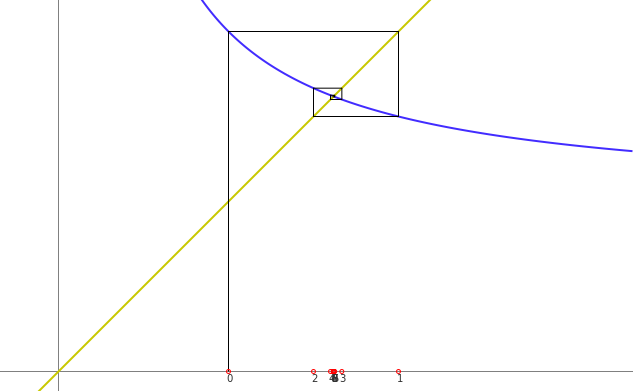
\includegraphics[width=\textwidth]{fig_fibonacci.png}
  \end{center}
  \caption{Diagramma a ragnatela relativo
    all'esercizio~\ref{ex_fibonacci}.}
  \label{fig_fibonacci}
\end{figure}

Un metodo grafico per visualizzare l'andamento dei termini della
successione definita da \eqref{eq1} è il \emph{diagramma a
  ragnatela}. Si disegna la curva $y=f(x)$ su un piano
cartesiano. Partendo dal punto di coordinate $(\alpha, 0)=(a_1, 0)$ si procede
lungo una retta verticale fino a raggiungere il grafico della funzione
nel punto $(a_1, f(a_1)) = (a_1, a_2)$. Dopodiché si procede in
orizzontale fino ad incontrare la retta $y=x$ nel punto $(a_2,a_2)$ e
si ripete il procedimento in modo che le coordinate $x$ (ma anche le $y$)
dei vertici della spezzata mi danno la successione $a_1, a_2, a_3,
\dots$. Ad esempio il diagramma a ragnatela corrispondente
all'esercizio~\ref{ex_fibonacci} è rappresentato in
Figura~\ref{fig_fibonacci}.

\begin{exercise}\label{ex_3}
  Si consideri la successione definita per ricorrenza
  \[
  \begin{cases}
    a_1 = 0\\
    a_{n+1} =1 + a_n^2.
  \end{cases}
  \]
  Determinare il limite della successione.
\end{exercise}

\begin{figure}
  \myurl{ex3}{Diagramma a ragnatela relativo all'esercizio \getrefnumber{ex_3}}
  \begin{center}
    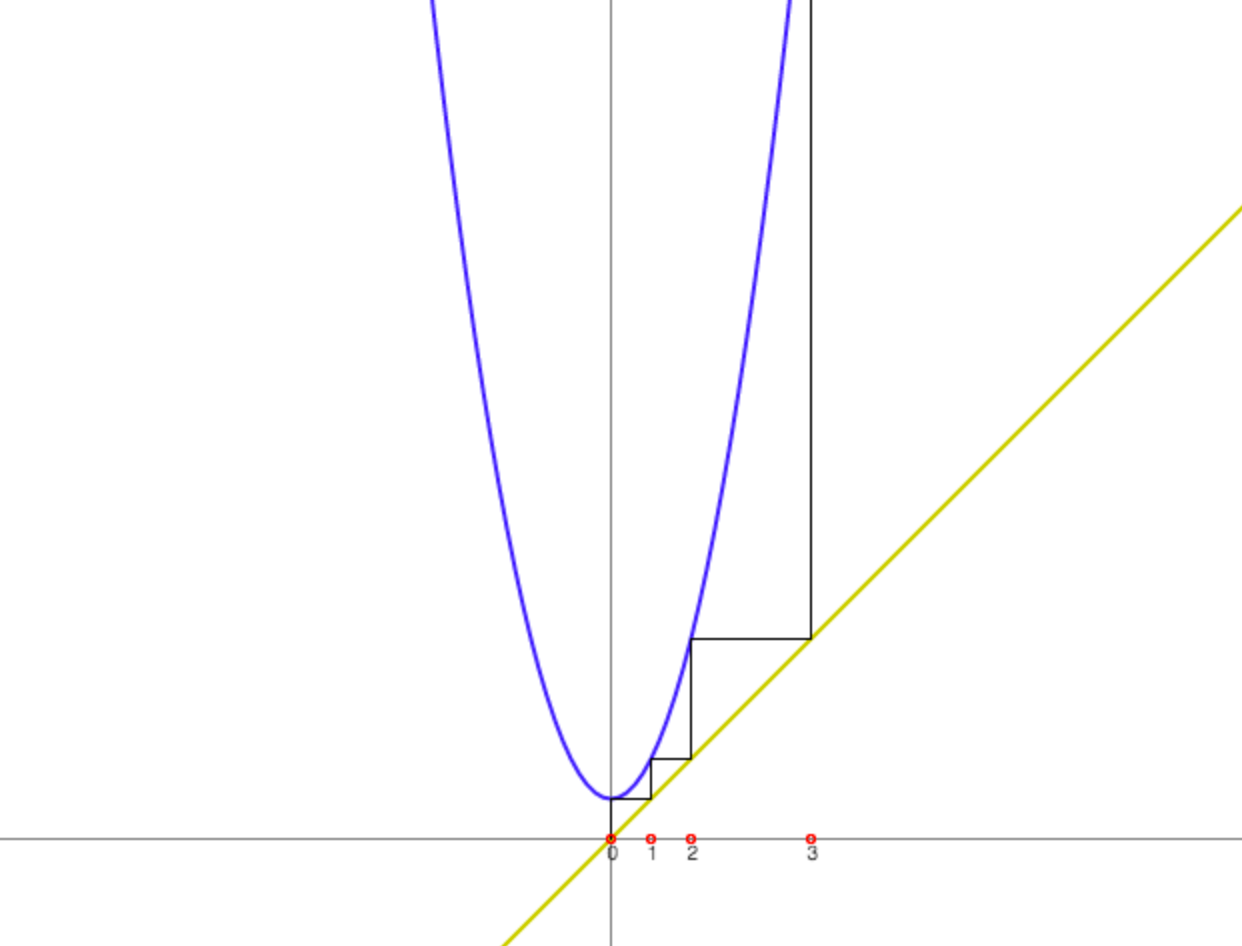
\includegraphics[width=\textwidth]{fig_ex_3.png}
  \end{center}
  \caption{Diagramma a ragnatela relativo
    all'esercizio~\ref{ex_3}.}
  \label{fig_ex_3}
\end{figure}

\begin{proof}[Soluzione]
  L'equazione ricorsiva è $a_{n+1}=f(a_n)$ se poniamo $f(x) = 1+x^2$.
  E' facile verificare che per ogni $x$ si ha $f(x) > x$ e quindi, per
  il Teorema~\ref{th_1} otteniamo che la successione $a_n$ è
  crescente. Dunque ammette limite: $a_n \to \ell$. Se il limite fosse
  finito si avrebbe
  \[
  a_{n+1} = 1 + a_n^2 \to 1 + \ell
  \]
  e quindi, visto che $a_{n+1}\to \ell$, si avrebbe $\ell = 1 +
  \ell^2$ (cioè $\ell$ dovrebbe essere un punto fisso di $f$). Questa
  equazione abbiamo già osservato che non ha soluzioni ($x^2 + 1 > x$)
  e quindi $\ell$ non è finito. Visto che la successione $a_n$ è
  crescente possiamo escludere che sia $\ell=-\infty$ e quindi l'unica
  possibilità che rimane è che $a_n \to +\infty$.
\end{proof}

\begin{figure}
  \myurl{ex4}{Diagramma a ragnatela relativo all'esercizio \getrefnumber{ex_4}}
  \begin{center}
  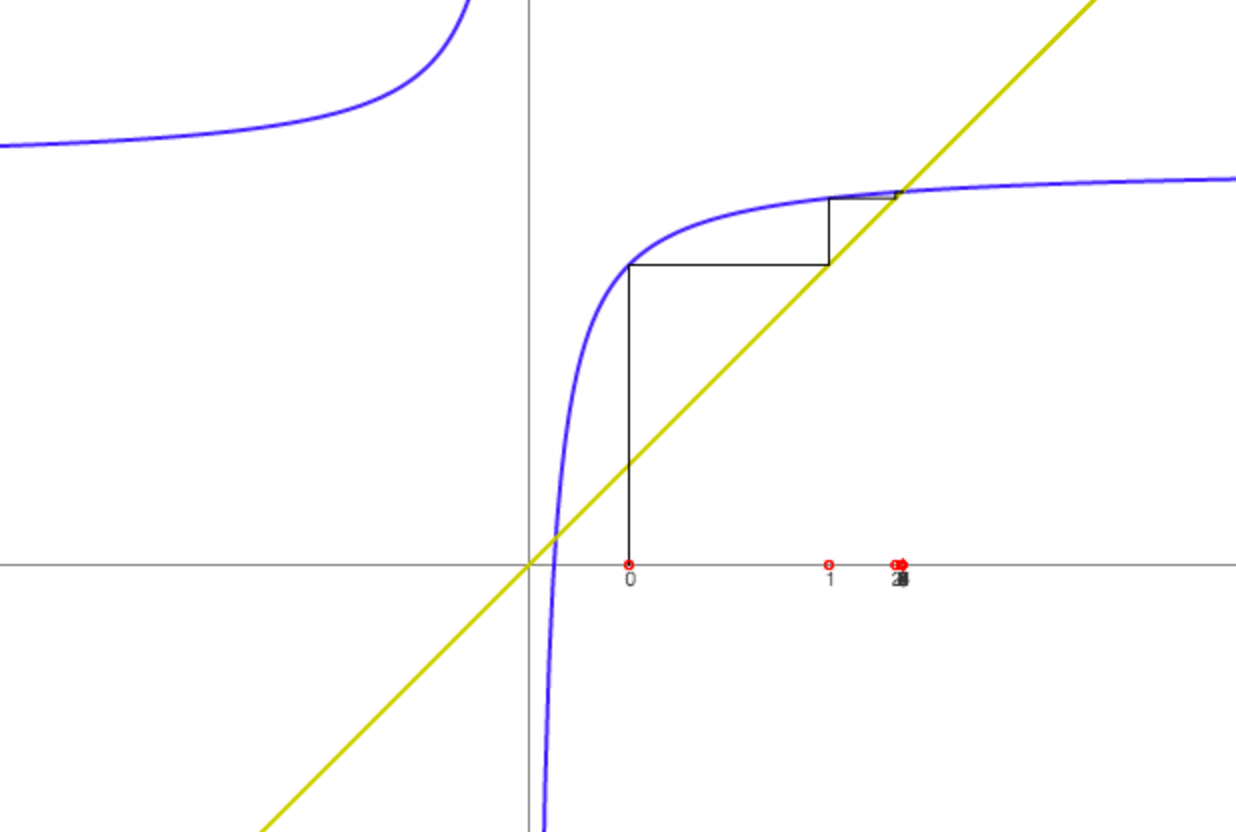
\includegraphics[width=\textwidth]{fig_ex_4.png}
  \end{center}
  \caption{Diagramma a ragnatela relativo
    all'esercizio~\ref{ex_4}.}
  \label{fig_ex_4}
\end{figure}

\begin{exercise}\label{ex_4}
  Si consideri la successione definita per ricorrenza
  \[
  \begin{cases}
    a_1 = 1\\
    a_{n+1} =4-\frac 1 {a_n}.
  \end{cases}
  \]
  Determinare il limite della successione.
\end{exercise}

\begin{proof}[Soluzione.]
  Si mostra che sull'intervallo $A=(2-\sqrt 3, 2+\sqrt 3)$
  vale $f(x)>x$, che gli estremi di $A$ sono punti fissi
  e inoltre che la funzione $f$ è crescente (lo è su tutto $(0,+\infty)$).
  Di conseguenza è facile verificare che $A$ è invariante, in quanto si ha
  \begin{align*}
  2-\sqrt 3 < x < 2+\sqrt 3 &\Rightarrow
  f(2-\sqrt 3) < f(x) < f(2+\sqrt 3)\\
  &\Rightarrow
  2-\sqrt 3 < f(x) < 2+\sqrt 3.
  \end{align*}

  Inoltre se $a_1 \in A$ allora per ogni $n\ge 1$ si ha $a_n\in A$ ed essendo
  $f(x)>x$ la successione sarà crescente. Dunque ammette
  limite: $a_n \to \ell \in \bar A$, $\ell \ge a_1$. Ma allora
  \[
  a_{n+1} = 4-\frac 1 {a_n} \to 4 - \frac 1 \ell = f(\ell)
  \]
  e visto che $a_{n+1}$ ha lo stesso limite di $a_n$ si ha $\ell =
  f(\ell)$ le cui uniche soluzioni sono $2\pm \sqrt 3$. Ma $2-\sqrt 3$
  va scartata in quanto $\ell\ge a_1 > 2-\sqrt 3$ e quindi rimane
  $a_n \to \ell = 2+\sqrt 3$.
\end{proof}

\begin{figure}
 \myurl{ex5}{Diagramma a ragnatela relativo all'esercizio \getrefnumber{ex_5}}
 \begin{center}
    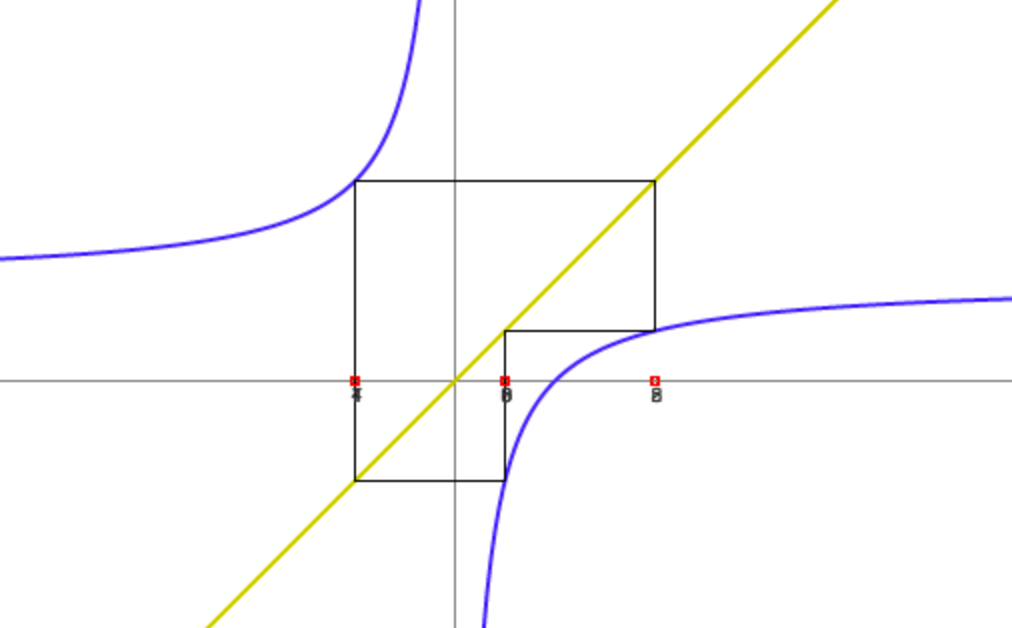
\includegraphics[width=\textwidth]{fig_ex_5.png}
  \end{center}
  \caption{Diagramma a ragnatela relativo
    all'esercizio~\ref{ex_5}.}
  \label{fig_ex_5}
\end{figure}

\begin{exercise}\label{ex_5}
  Si consideri la successione definita per ricorrenza
  \[
  \begin{cases}
    a_1 = \frac 1 2\\
    a_{n+1} = 1- \frac{1}{a_n}
  \end{cases}
  \]
  Determinare, se esiste, il limite della successione.
\end{exercise}

\begin{proof}[Soluzione.]
  Osserviamo che:
  \begin{align*}
    a_1 &= \frac 1 2 \\
    a_2 &= 1 - \frac{1}{1/2} = -1\\
    a_3 &= 1 - \frac{1}{-1} = 2\\
    a_4 &= 1 - \frac{1}{2} = \frac 1 2 = a_1
  \end{align*}
  Essendo $a_4 = a_1$ la successione si ripete e, (per induzione) si
  dimostra che $a_{3n+k} = a_k$. Dunque si ha
  \begin{align*}
    a_{3n} &= a_3 = 2 \to 2\\
    a_{3n+1} &= a_1 = 1/2 \to 1/2\\
    a_{3n+2} &= a_2 = -1 \to -1
  \end{align*}
  e la successione $a_n$ non ammette limite.
\end{proof}

\begin{figure}
  \myurl{ex6}{Diagramma a ragnatela relativo all'esercizio \getrefnumber{ex_6}}
  \begin{center}
    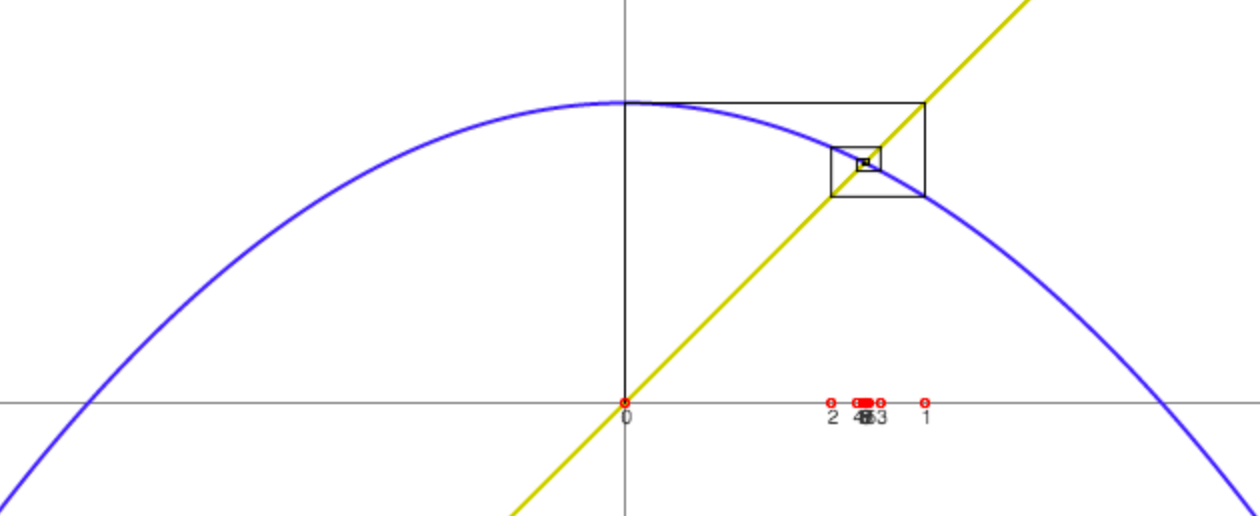
\includegraphics[width=\textwidth]{fig_ex_6.png}
  \end{center}
  \caption{Diagramma a ragnatela relativo
    all'esercizio~\ref{ex_6}.}
  \label{fig_ex_6}
\end{figure}

\begin{exercise}\label{ex_6}
  Si consideri la successione definita per ricorrenza
  \[
  \begin{cases}
    a_1 = 0\\
    a_{n+1} = \frac{5-a_n^2}{4}.
  \end{cases}
  \]
  Determinare il limite della successione.
\end{exercise}

\begin{proof}[Soluzione.]
Si ha $a_{n+1} = f(a_n)$ se scegliamo $f(x) = (5-x^2)/4$. Osserviamo
che la funzione $f$ è decrescente per $x \ge 0$ (infatti $0 \le x_1 <
x_2$ implica $x_1^2 < x_2^2$ da cui $-x_1^2 > -x_2^2$ e quindi $f(x_1)
> f(x_2)$). Osserviamo inoltre che
\begin{align*}
a_1 &= 0\\
a_2 &= f(a_1) = 5/4.\\
a_3 &= f(5/4) = \frac{5-25/16}{4} = \frac{55}{64}
\end{align*}
Vogliamo dimostrare che l'intervallo $A=[0,5/4]$ è invariante. Visto
che $f$ è decrescente su tale intervallo, si ha:
\begin{align*}
0 \le x \le \frac 5 4 &\Rightarrow f(0) \ge f(x) \ge f(5/4)\\
&\Rightarrow \frac 5 4 \ge f(x) \ge \frac{55}{64} \ge 0\\
&\Rightarrow 0 \le f(x) \le \frac 5 4
\end{align*}
cioè $x\in A \Rightarrow f(x)\in A$, che è quanto volevamo dimostrare.

Per il Teorema~\ref{th_decr} sappiamo dunque che $a_{2n} \to \ell$ e
$a_{2n+1} \to \ell'$. Entrambi i limiti sono finiti in quanto essendo
$a_n \in A$ per ogni $n$, si ha $\ell, \ell' \in \bar A = A$.
Dunque, come al solito, osserviamo che si ha:
\begin{align*}
  a_{2n+1} &= f(a_n) \to f(\ell)  \\
  a_{2n+2} &= f(a_{n+1}) \to f(\ell')
\end{align*}
ma sapendo che $a_{2n+1}\to \ell'$ e $a_{2n+2}\to \ell$ otteniamo il
seguente sistema:
\[
\begin{cases}
  \ell' = f(\ell)\\
  \ell = f(\ell')
\end{cases}
\]
da cui si ottiene $f(f(\ell))=\ell$ e $f(f(\ell'))=\ell'$. Dunque
vogliamo scrivere e risolvere l'equazione $f(f(x))=x$:
\[
\frac{5-\left(\frac{5-x^2}{4}\right)^2}{4} = x
\]
cioè
\[
5 - \frac{25 - 10x^2 + x^4}{16} = 4x
\]
ovvero
\[
x^4 - 10 x^2 + 64 x - 55 = 0.
\]

Come facciamo a risolvere una equazione di quarto grado?
In questo frangente dobbiamo fare una osservazione di carattere
generale che ci sarà di grande aiuto.
Osserviamo che se $x$ è una soluzione di $f(x)=x$ allora $x$
è anche soluzione di $f(f(x)) = x$ in quanto in tal caso si ha
$f(f(x))=f(x)=x$.
Ma l'equazione $f(x) = x$ è una equazione di secondo grado, che quindi
possiamo facilmente risolvere:
\begin{gather*}
  \frac{5-x^2}{4} = x \\
  x^2 + 4x - 5 = 0 \\
  x_{12} = -2 \pm \sqrt{4 + 5} = -2 \pm 3.
\end{gather*}

Dunque abbiamo trovato due zeri del polinomio di quarto grado e quindi
tale polinomio deve essere divisibile per
\[
 x^2 + 4x - 5 = (x-1)(x+5).
\]
Eseguiamo la divisione tra polinomi:
\begin{align*}
\frac{x^4 - 10 x^2 + 64 x - 55}{x^2 + 4x - 5}
&= x^2 + \frac{x^4 - 10 x^2 + 64x - 55 - x^2 (x^2 + 4x - 5)}{x^2+4x-5}\\
&= x^2 + \frac{-4x^3 - 5 x^2 + 64 x - 55}{x^2+4x-5}\\
&= x^2 - 4x + \frac{-4x^3 - 5x^2 - 64 x - 55 + 4x(x^2+4x-5)}{x^2+4x-5}
\\
&= x^2 - 4x + \frac{11 x^2 + 44 x - 55}{x^2 + 4x -5}\\
&= x^2 - 4x + 11.
\end{align*}
Come previsto la divisione non ha resto. Possiamo quindi completare la
scomposizione cercando gli zeri del polinomio $x^2-4x+11$ che però, da
un rapido controllo, non ha soluzioni reali.

Dunque in questo caso i punti fissi di $f$ coincidono con i punti
fissi di $f\circ f$ e dunque i due limiti $\ell, \ell'$ devono essere
elementi dell'insieme dei punti fissi: $\ENCLOSE{1, -5}$. D'altra parte $-5$
deve essere escluso in quanto i limiti stanno entrambi nella chiusura
dell'insieme invariante, che non comprende numeri negativi.

Concludiamo quindi che $\ell = \ell' = 1$ e dunque l'intera
successione ha limite: $a_n \to 1$.
\end{proof}

\begin{exercise}\label{ex_7}
  Si consideri la successione definita per ricorrenza
  \[
  \begin{cases}
    a_1 = \alpha\\
    a_{n+1} = 2- a_n^2.
  \end{cases}
  \]
  Determinare il limite della successione nei casi: $\alpha=-7$, $\alpha=4$ e $\alpha=1/42$.
\end{exercise}

\begin{figure}
 \myurl{ex7}{Diagramma a ragnatela relativo all'esercizio \getrefnumber{ex_7}}
   \begin{center}
    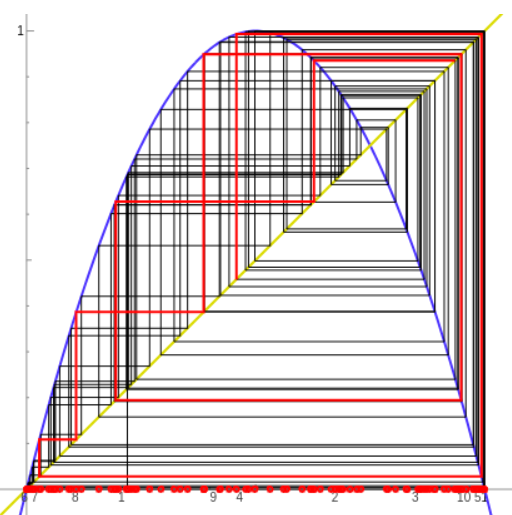
\includegraphics[width=\textwidth]{fig_ex_7.png}
  \end{center}
  \caption{Diagramma a ragnatela relativo
    all'esercizio~\ref{ex_7}.}
  \label{fig_ex_7}
\end{figure}

\begin{proof}[Soluzione.]
  Abbiamo $a_{n+1} = f(a_n)$ con $f(x) = 2-x^2$. Determiniamo i punti
  fissi di $f$:
  \[
  2-x^2 = x, \qquad x^2 + x - 2 = 0
  \]
  che ha come soluzioni $x_{1,2} = \frac{-1\pm\sqrt{1+8}}{2}$ cioé
  $x_1 = -2$, $x_2 = 1$. Tenendo conto anche dei segni si può
  osservare che all'interno delle due soluzioni si ha $f(x)>x$ mentre
  all'esterno si ha $f(x)<x$.

  Osserviamo inoltre che $f(x)$ è crescente per
  $x\le 0$ e decrescente per $x\ge 0$.

  Caso $\alpha=-7$. In questo caso consideriamo l'intervallo
  $A=(-\infty, -2)$. Visto che $f$ è crescente su questo intervallo,
  e visto che $-2$ è un punto fisso si ha:
  \[
  x < -2 \Rightarrow f(x) < f(-2) \Rightarrow f(x) < -2
  \]
  che significa che $A$ è un intervallo invariante.

  Su questo intervallo si ha $f(x)<x$ e quindi $a_n$ è decrescente e
  di conseguenza ammette limite $a_n\to \ell$. Il limite può essere
  finito oppure $-\infty$. Ma se fosse finito allora avremmo
  \[
  a_{n+1} = 2 - a_n^2 \to 2 - \ell^2
  \]
  e siccome $a_{n+1}\to \ell$ avremmo $\ell = 2 - \ell^2$ cioè $\ell$
  è un punto fisso di $f$. Ma visto che $\ell \le a_1 = \alpha < x_1 <
  x_2$ otteniamo un assurdo.

  Dunque l'unica possibilità è che $a_n \to -\infty$. Questo
  stesso ragionamento vale per ogni $\alpha<-2$.

  Caso $\alpha=4$. In questo caso si ha:
  \begin{align*}
    a_1 &= \alpha = 4\\
    a_2 &= f(a_1) = 2 - 4^2 = -14.
  \end{align*}
  quindi $a_2 \in A$ (l'intervallo invariante del punto precedente) e
  dall'indice $2$ in poi ci si riconduce quindi ai risultati
  precedenti. Dunque anche in questo caso $a_n \to -\infty$.

  Caso $\alpha = 1/42$. Questo caso è decisamente più complesso dei
  precedenti. Prendiamo l'insieme $A_2 = [-2, 2]$, vogliamo dimostrare
  che è un insieme invariante. Nell'intervallo $[-2,0]$ la funzione è
  crescente e quindi ha minimo in $-2$ dove vale $f(-2)=-2$ ed ha
  massimo in $0$ dove assume il valore $f(0) = 2$. Nell'intervallo
  $[0,2]$ la funzione è decrescente e, di nuovo, ha massimo $f(0)=2$ e
  minimo $f(2)=-2$. Dunque per ogni $x\in [-2,2]$ si ha $f(x) \in
  [-2,2]$ cioè, come volevamo dimostrare, $A_2$ è invariante.

  Dunque visto che $a_1 = \alpha \in A_2$ scopriamo che per ogni $n$
  si ha $a_n \in [-2,2]$. Supponiamo ora che la successione abbia
  limite: $a_n \to \ell$. In tal caso, passando al limite
  nell'equazione $a_{n+1} = f(a_n)$ otteniamo, come al solito, che il
  limite dovrebbe essere un punto fisso di $f$: o $\ell=-2$ o
  $\ell=1$. Cercheremo ora di dimostrare che questo è assurdo. Ci sono
  due possibilità che dobbiamo escludere. La prima è che la
  successione tenda al punto fisso $\ell$ senza mai uguagliarlo. La
  seconda è che per un certo $n_0$ si abbia $a_n = \ell$ per $n=n_0$ e
  quindi per ogni $n\ge n_0$.

  Supponiamo di essere nel primo caso e supponiamo che $\ell = -2$. In
  tal caso, per il teorema della permanenza del segno la successione
  deve, da un certo indice in poi, stare nell'intervallo $[-2, 0]$. Ma
  in tale intervallo si ha $f(x)>x$ e quindi la successione sarebbe,
  da un certo indice in poi, crescente. Ma visto che $a_n \ge -2$ per
  ogni $n$ non è possibile che la successione converga, crescendo, a
  $-2$.

  Supponiamo allora di essere nel primo caso (la successione è sempre
  diversa dai due punti fissi) e supponiamo che $\ell = 1$. In
  questo caso da un certo indice in poi la successione deve stare
  nell'intervallo $[0,2]$ (altrimenti non potrebbe convergere a
  $1$. In tale intervallo la funzione $f$ è decrescente e quindi
  le sottosuccessioni dei termini pari e dei termini dispari sono
  entrambe monotone. Si potrebbe cercare di studiare le successioni dei
  termini pari $a_{2n}$ e dispari $a_{2n+1}$ che soddisfano una relazione di ricorrenza
  con la funzione $f\circ f$ al posto di $f$ e osservare che la successione
  che si trova a sinistra del punto fisso dovrebbe decrescere e quella che si trova a
  destra dovrebbe crescere (e questo sarebbe assurdo). Un metodo forse più
  rapido che non richiede lo studio della funzione composta è invece il seguente.
  L'idea è di osservare che $f$ tende ad aumentare le distanze quando ci si trova
  nei paraggi del punto $1$. Se per assurdo $a_n\to 1$ allora definitivamente
  si dovrà avere $\abs{a_n-1}< 1/2$. Ma allora si osserva che:
  \[
    \abs{a_{n+1}-1}
    = \abs{2-a_n^2-1}=\abs{1-a_n^1}
    = \abs{1+a_n}\cdot \abs{1-a_n}
    \ge \frac 3 2 \abs{a_n-1}
  \]
  in quanto se $\abs{a_n-1}<1/2$ allora (per la disuguaglianza triangolare inversa)
  $\abs{1+a_n}\ge 3/2$. Questo è assurdo perché significa che $\abs{a_n -1}\to +\infty$
  (per il criterio del rapporto) quando invece dovrebbe essere $\abs{a_n-1}\to 0$.

  \textbf{Nota.} Vedremo nei prossimi teoremi che
  se la derivata di $f$ è in valore assoluto minore di
  $1$ allora il punto fisso sarà stabile (o attrattivo) cioè partendo
  da un punto sufficientemente vicino si convergerà necessariamente al
  punto fisso. Se invece la derivata è in valore assoluto maggiore di
  $1$ il punto fisso sarà instabile (o repulsivo). Cioè, a parte la
  successione costante che assume il valore esatto del punto fisso,
  non è
  possibile che una successione converga al punto fisso.

  Rimane da considerare la possibilità che la successione assuma da un
  certo punto in poi il valore esatto di un punto fisso. Supponiamo ad
  esempio che per un certo $n$ si abbia $a_n=1$. Allora si deve avere
  \[
  1 = a_n = 2-(a_{n-1})^2
  \]
  da cui
  \[
  a_{n-1} = \pm 1.
  \]
  Se $a_n$ era il primo termine con valore $1$ dovrà necessariamente
  essere $a_{n-1} = -1$. Ma allora
  \[
  -1 = a_{n-1} = 2-(a_{n-2})^2
  \]
  da cui $a_{n-2} = \pm \sqrt 3$. Ma ora osserviamo che essendo $a_1=
  \alpha = 1/42$ un numero razionale, e osservando che $\QQ$ è un
  insieme invariante per $f$ (perché? verificare per induzione...)
  sappiamo che ogni $a_k \in \QQ$ e quindi
  avremmo $a_{n_2} = \sqrt 3 \in \QQ$: assurdo.

  Stesso discorso si può fare se si avesse $a_n=-2$, in quanto si
  avrebbe $a_{n-1} = 2$, $a_{n-2} = 0$ e quindi $a_{n-3}=\pm \sqrt 2$.

  Dunque la successione $a_n$ non ammette limite.
\end{proof}

\begin{exercise}\label{ex_8}
  Si consideri la successione definita per ricorrenza
  \[
  \begin{cases}
    a_1 = \alpha\\
    a_{n+1} = \frac{1}{2-a_n}.
  \end{cases}
  \]
  Trovare il limite della successione nel caso $\alpha =
  -\the\year$. Determinare l'insieme dei valori di $\alpha$ per i quali la
  successione $a_n$ non è ben definita (in quanto per un qualche $n$ il
  denominatore $2-a_n$ si annulla).
  Trovare il limite nel caso $\alpha=\frac{\the\year}{1000}$.
\end{exercise}

\begin{figure}
 \myurl{ex8}{Diagramma a ragnatela relativo all'esercizio \getrefnumber{ex_8}}
 \begin{center}
    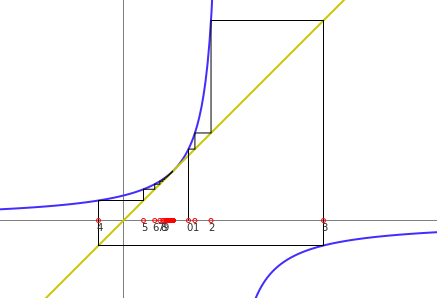
\includegraphics[width=\textwidth]{fig_ex_8.png}
  \end{center}
  \caption{Diagramma a ragnatela relativo
    all'esercizio~\ref{ex_8}.}
  \label{fig_ex_8}
\end{figure}

\begin{proof}[Soluzione.]
Posto $f(x) = 1/(2-x)$
si osserva che la disequazione $f(x)\ge x$ è verificata per ogni
$x<2$. L'equazione di punto fisso $f(x)=x$ ha come unica soluzione
$x=1$. Sull'intervallo $A=(-\infty,1)$ la funzione $f$ è crescente e
l'intervallo risulta essere invariante. Dunque per
$\alpha=-\the\year \in A$ la successione risulta essere crescente e superiormente
limitata. Dunque converge $a_n\to \ell$. Passando al limite in
$a_{n+1} = f(a_n)$ si trova che $\ell$ deve essere un punto fisso di
$f$ e quindi $\ell = 1$.

La successione non è ben definita se per qualche $n$ si trovasse
$a_n=2$ in quanto la funzione $f$ non è definita per $x=2$. Altri
valori si ottengono risalendo all'indietro la successione $a_n$.
Dalla equazione
\[
a_n = \frac{1}{2-a_{n-1}}
\]
si ricava
\[
a_{n-1} = 2-\frac{1}{a_n}.
\]
L'insieme dei punti partendo da quali si arriva prima o poi in $x=2$ è
dato dunque dai valori della successione
\[
\begin{cases}
  b_1 = 2\\
  b_{n+1} = 2 - \frac{1}{b_n}.
\end{cases}
\]
Osserviamo che in questo caso specifico è possibile ricavare una
formula esplicita per il termine $b_n$. Osserviamo infatti che:
\[
b_1 = 2,\quad
b_2 = \frac{3}{2},\quad
b_3 = \frac{4}{3}
\]
e proviamo a congetturare che sia $b_n = (n+1) / n$. In effetti questo
si può dimostrare per induzione. Per $n=1$ si ha $(n+1)/n = 2 =
b_1$. E se supponiamo che valga $b_n = (n+1)/n$ si ha
\[
b_{n+1} = 2 - \frac{n}{n+1} = \frac{2n+2-n}{n+1} = \frac{n+2}{n+1}.
\]
Dunque l'insieme dei punti partendo dai quali la successione $a_n$ non
è ben definita è dato da:
\[
  X= \ENCLOSE{\frac{n+1}{n}\colon n \in \NN}.
\]

Per il caso $\alpha=\frac{\the\year}{1000}$ osserviamo che sull'intervallo
$A_2 = (1,2)$ si ha sempre $f(x)>x$ (ma si potrebbe osservare che
$A_2$ non è invariante). Finché $a_n$ rimane in
tale intervallo la successione risulta quindi crescente. Però non è
possibile che la successione rimanga sempre in $A_2$ perché in tal
caso il limite dovrebbe essere un punto
fisso. Ma l'unico punto fisso è $1$ che è minore di $\alpha$ e quindi
la successione, crescente, non può convergere. Necessariamente la
successione esce dall'intervallo $A_2$ (in effetti notiamo che $\alpha
\not \in X$) e, per un certo $n$ si avrà $a_n>2$. Osserviamo ora che
sull'intervallo $A_3 = (2,+\infty)$ si ha $f(x)<0$ e dunque
se $a_n\in A_2$ necessarimante $a_{n+1} \in A$. Dunque questo caso si
riconduce al primo studiato, e la successione tende a $1$.
\end{proof}

\begin{exercise}
  Si consideri la successione definita per ricorrenza
  \[
  \begin{cases}
    a_1 = \alpha\\
    a_{n+1} = \frac{a_n^2-a_n}{2}.
  \end{cases}
  \]
  Determinare al variare di $\alpha$ il limite della successione.
\end{exercise}

\begin{exercise}
  Si consideri la successione definita per ricorrenza
  \[
  \begin{cases}
    a_1 = \alpha \\
    a_{n+1} = 1 - a_n^2.
  \end{cases}
  \]
  Determinare al variare di $\alpha$ il limite della successione.
\end{exercise}

\begin{exercise}
Calcolare
\[
 1 + \frac{1}{1+\frac{1}{1+\frac{1}{1+\frac{1}{\dots}}}}
\]
\end{exercise}

\begin{exercise}
Calcolare
\[
  \lim_{x\to 1^+} \sqrt{x-\sqrt{x- \sqrt{x-\sqrt{x - \dots}}}}
\]
\end{exercise}

\begin{exercise}[Mandelbrot reale]
\label{ex:mandelbrot_reale}
Si consideri, fissato il parametro $c$, la successione definita per ricorrenza:
\[
  \begin{cases}
    a_0 = 0\\
    a_{n+1} = a_n^2 + c.
  \end{cases}
\]

Determinare i valori di $c\in \RR$ per i quali la successione $a_n$ risulta
essere limitata.
\end{exercise}
%
\begin{proof}[Svolgimento.]
\emph{Caso 1: $c > \frac 1 4$}.
In tal caso non ci sono punti fissi, in quanto l'equazione $x=x^2+c$ ha
discriminante negativo. Significa che $x^2+c > x$ per ogni $x\in \RR$. Dunque
la successione $a_n$ è strettamente crescente e tende a $+\infty$.
Non è limitata.

\emph{Caso 2:} $0\le c \le \frac 1 4$.
In questo caso l'equazione $x=x^2+c$ ha due soluzioni entrambe positive
(le soluzioni hanno somma $1$ e prodotto $c\ge 0$).
Se chiamiamo $x_1$ la più piccola delle due soluzioni possiamo dimostrare che
l'intervallo $[0,x_1)$ è invariante. Infatti su tali intervallo la funzione
$f(x)=x^2+c$ è crescente, dunque se $0\le x < x_1$ si ha $f(0) \le f(x) < f(x_1)$
cioè $c \le f(x) < x_1$. Visto che $c\ge 0$ abbiamo mostrato che l'intervallo è
invariante e la successione è dunque limitata.
Se $c=0$ la successione $a_n$ rimane costante $a_n=0$. Se $c>0$ la successione
converge al punto fisso $x_1$. In ogni caso è limitata.

\emph{Caso 3:} $-1 \le c < 0$.
In questo caso vogliamo mostrare che l'intervallo $[c,0]$ è invariante.
La funzione $f(x) = x^2+c$ è decrescente su tale intervallo, dunque
se $c\le x \le 0$ risulta $f(0)\le x \le f(c)$. Ma $f(0)=c$ e $f(c)=c^2+c
= c(c+1) \le 0$ se $c\ge -1$. Dunque $[c,0]$ è invariante e $a_n$ rimane
limitata in tale intervallo.

\emph{Caso 4:} $-2\le c < -1$.
In questo caso l'equazione $x=x^2+c$ ha una soluzione negativa ed una soluzione
positiva. Chiamiamo $x_2$ la soluzione positiva. Vogliamo mostrare che
l'intervallo $[c,x_2]$ è invariante.
La funzione $f(x)=x^2+c$ è decrescente in $[c,0]$ e crescente in $[0,x_2]$.
Se $0\le x \le x_2$ si ha dunque $f(0)\le f(x) \le f(x_2)$
cioè $c \le f(x) \le x_2$. Dunque i punti in $[0,x_2]$ rimangono nell'intervallo
$[c,x_2]$.
Se invece $c\le x \le 0$ si ha $f(0)\le f(x) \le f(c)$ cioè $c \le f(x) \le c^2+c$.
Affinché sia $c^2+c\le x_2$ basta verificare che $f(c^2+c)\le c^2+c$
cioè:
\[
  (c^2+c)^2 + c \le c^2+c
\]
che, sviluppando il quadrato, si riduce a $c^3(c+2)\le 0$ che è verificata
se $-2 \le c \le 0$.
Dunque l'intervallo $[c,x_2]$ è invariante. La successione rimane dunque
limitata in tale intervallo.

\emph{Caso 5:} $c < -2$.
In questo caso $a_0=0$, $a_1=c$, $a_2=c^2+c$ e possiamo verificare che
$c^2+c > x_2$ in quanto, come nel caso precedente, questo accade se
\[
   (c^2+c)^2 + c > c^2+c
\]
che si riduce a $c^3(c+2)>0$ che è verificata se $c<-2$.
Ma l'intervallo $(x_2,+\infty)$ è invariante e su tale intervallo
si ha $f(x)>x$ dunque la successione $a_n$ è strettamente crescente per $n\ge 2$
e diverge a $+\infty$. Non è dunque limitata.

\emph{Conclusione}. La successione è limitata se $c\in[-2,1/4]$.
Altrimenti $a_n\to +\infty$.

\end{proof}

\section{approfondimenti}

I risultati esposti finora non richiedevano
alcuna nozione del calcolo differenziale
e potevano essere compresi utilizzando solamente
le nozioni del capitolo~\ref{ch:successioni}.
In questo capitolo useremo invece
alcuni concetti che riguardano il calcolo differenziale.

\begin{theorem}[criterio per la stabilità di un punto fisso]
Sia $x_0\in \RR$, $R>0$, $I=(x_0 - R, x_0+R)$ e $f\colon I \to \RR$
una funzione che ha $x_0$ come punto fisso.
Se $f$ è $L$-lipschitziana su $I$ con $L<1$ allora $I$ è un intervallo
invariante per $f$ e se $a_n$ è una successione che soddisfa la relazione di ricorrenza $a_{n+1} = f(a_n)$ con $a_0 \in I$
allora $a_n \to x_0$ per $n\to +\infty$.

In particolare se $f\in C^1(I)$ con punto fisso $x_0 \in I$ e $\sup\ENCLOSE{\abs{f'(x)}\colon x\in I} < 1$ allora $I$ è invariante ed ogni successione $a_n$ definita per ricorrenza da $a_{n+1}=f(a_n)$ con $a_0 \in I$ converge ad $x_0$.

Ancora più in particolare, se $f$ è di classe $C^1$ in un intorno di un punto $x_0$, se $x_0$ è punto fisso di $f$ e $\abs{f'(x_0)}<1$ allora
esiste un intorno $I$ di $x_0$ che è invariante per $f$ e ogni successione $a_n$ definita per ricorrenza tramite $a_{n+1}= f(a_n)$ con $a_0\in I$ converge ad $x_0$.
\end{theorem}
  %
\begin{proof}
Osserviamo che se $f$ è di classe $C^1$ in un intorno di $x_0$ e $\abs{f'(x_0)} < 1$ allora, per continuità, esiste $L<1$ tale $\abs{f'(x)} < L$ per ogni $x$ in un intorno $I$ di $x_0$. Dunque $\sup\ENCLOSE{\abs{f'(x)}\colon x \in I} \le L < 1$ e la funzione $f$ risulta dunque essere $L$-lipschitziana. E' chiaro quindi che la seconda e la terza parte del teorema si riconducono alla prima, che è quella che andremo ora a dimostrare.

Se $f$ è $L$-lipschitziana e $x_0$ è punto fisso di $f$ osserviamo che si ha
\[
\abs{f(x) - x_0} = \abs{f(x) - f(x_0)} \le L \abs{x-x_0}
\]
da cui se $\abs{x - x_0} < R$ anche $\abs{f(x) - x_0} < R$.
Dunque $I = (x_0-R, x_0+R)$ è invariante.
Possiamo poi dimostrare per induzione che risulta
\[
 \abs{a_n - x_0} \le L^n \cdot \abs{a_0-x_0}.
\]
Infatti per $n=0$ la relazione è una uguaglianza. Il passo induttivo si ottiene osservando che
\begin{align*}
\abs{a_{n+1} - x_0}
 &= \abs{f(a_n) - f(x_0)}
 \le L \abs{a_n - x_0} \\
 &\le L\cdot L^n\abs{a_0-x_0}
 = L^{n+1}\abs{a_0-x_0}.
\end{align*}

Ma ora se $L<1$ si ha $L^n\to 0$ e dunque $\abs{a_n -x_0} \to 0$ come volevamo dimostrare.
\end{proof}

\begin{theorem}[instabilità del punto fisso]
Sia $f$ di classe $C^1$ in un intorno di un suo punto fisso $x_0$.
Se $\abs{f'(x_0)}>1$ allora non esiste una successione $a_n$ che soddisfa la relazione ricorsiva $a_{n+1} = f(a_n)$ e tale che $a_n \to x_0$ a meno che non si abbia $a_n = x_0$ da un certo indice $n$ in poi.
\end{theorem}
%
\begin{proof}
Per continuità della derivata esisterà $L>1$ e un intervallo $I$
intorno di $x_0$ tale che per ogni $x\in I$ si abbia $\abs{f'(x)} > 1$.
Se $a_n \to x_0$ allora da un certo indice $n$
in poi si avrà $a_n \in I$.
Se $a_n$ verifica la relazione ricorsiva $a_{n+1} = f(a_n)$ possiamo
allora applicare il teorema di Lagrange per ottenere che per ogni $n$ esiste $b_n$ compreso tra $x_0$ e $a_n$ tale che:
\begin{align*}
  \abs{a_{n+1} - x_0}
  &= \abs{f(a_n) - f(x_0)}
  = \abs{f'(b_n)(a_n - x_0)} \\
  &\ge L \cdot \abs{a_n - x_0} \ge \abs{a_n - x_0}.
\end{align*}
Risulta quindi che la distanza $\abs{a_n - x_0}$ deve essere crescente
e quindi l'unica possibilità perché $a_n \to x_0$ è che sia $a_n = x_0$.
\end{proof}

\section{equazioni ricorsive lineari}
\label{sec:ricorrenza_lineare}

Fissate le costanti $c_0, c_1, \dots, c_n$,
con $c_n \neq 0$,
diremo che l'equazione ricorsiva:
\begin{equation}\label{eq:ricorsione_lineare}
  c_n \cdot a_{k+n} + c_{n-1} \cdot a_{k+n-1} + \dots
    + c_1 \cdot a_{k+1} + c_0 \cdot a_k = 0
\end{equation}
è una \myemph{equazione!ricorsiva!lineare} (omogenea) di ordine $n$.
Il polinomio $P$ con gli stessi coefficienti:
\[
  P(\lambda) = c_n \cdot \lambda^n + c_{n-1}\cdot \lambda^{n-1} + \dots + c_1 \cdot \lambda + c_0
\]
si chiama \myemph{polinomio caratteristico}
\index{equazione!ricorsiva!lineare!polinomio caratteristico}
\index{polinomio!caratteristico!di una equazione ricorsiva lineare}%
associato all'equazione
lineare~\eqref{eq:ricorsione_lineare}.

Ad esempio la successione di Fibonacci $F_k$ definita da~\eqref{eq:Fibonacci}
è una soluzione dell'equazione ricorsiva lineare del secondo ordine:
\[
   a_{k+2} - a_{k+1} - a_{k} = 0
\]
il cui polinomio caratteristico è
\[
  P(\lambda) = \lambda^2 - \lambda - 1.
\]

\begin{theorem}[indipendenza delle successioni esponenziali]
\label{th:indipendenza_successioni_esponenziali}
Siano $\lambda_1, \dots, \lambda_n$ numeri complessi distinti. Allora
le successioni $\vec a_j$ definite da
\[
  \vec a_j (k) = \lambda_j^k
\]
sono vettori indipendenti nello spazio vettoriale complesso $\CC^\NN$ di tutte le
successioni a valori complessi.
\end{theorem}
%
\begin{proof}
Dobbiamo mostrare che se una combinazione lineare delle
successioni $\vec a_j$ è nulla allora tutti i coefficienti
sono nulli.
Supponiamo quindi di avere $c_1, \dots, c_n\in \CC$ tali che
\[
  \sum_{j=1}^n c_j \vec a_j = \vec 0 \in \CC^\NN.
\]
Significa che per ogni $k\in \NN$ si ha
\begin{equation}\label{eq:47862}
  \sum_{j=1}^n c_j \lambda_j^k = 0
\end{equation}
Dunque per ogni $k\in \NN$ e per ogni $z\in \CC$ si ha
\begin{equation}\label{eq:498137}
  \sum_{j=1}^n c_j \lambda_j^k z^k = 0.
\end{equation}
Sia ora $R=1/\max\ENCLOSE{\abs{\lambda_1}, \dots, \abs{\lambda_n}}$ (almeno uno dei $\lambda_j$
è non nullo perché i $\lambda_j$ sono distinti e possiamo assumere
$n>1$ altrimenti il teorema è banale).
Se $\abs{z}<R$ si ha $\abs{\lambda_j z}< 1$ per ogni $j$,
e la serie geometrica $\sum \lambda_j^k z^k$ risulta quindi essere
assolutamente convergente. Possiamo quindi fare la somma su $k$
dell'uguaglianza~\eqref{eq:498137}, scambiare le somme e ottenere,
per ogni $z$:
\[
  \sum_{j=1}^n \sum_{k=0}^{+\infty} c_j \enclose{\lambda_j z}^k = 0.
\]
Calcolando la somma della serie geometrica si ottiene, per ogni $z$
con $\abs{z}<R$:
\[
\sum_{j=1}^n \frac{c_j}{1-\lambda_j z} = 0.
\]
Scegliamo ora un indice $m$ cui $R = 1/\abs{\lambda_m}$ e
posto $z = t / \lambda_m$ osserviamo che per $t\in[0,1)$
si ha $\abs{z} < R$, dunque possiamo fare il limite
per $t\to 1^-$ ed ottenere :
\[
  \lim_{t\to 1^-}
  \sum_{j=1}^n \frac{c_j}{1- \lambda_j \frac{t}{\lambda_m} } = 0.
\]
Ma se $j\neq m$ si ottiene un limite finito:
\[
  \lim_{t\to 1^-} \frac{c_j}{1- \lambda_j \frac{t}{\lambda_m} }
  = \frac{c_j}{1 - \frac{\lambda_j}{\lambda_m}} = \ell_j \in \CC
\]
e dunque, visto che la somma dei limite è nulla,
anche per $j=m$ si deve ottenere un limite finito.
Ma per $j=m$ si ottiene invece
\[
  \lim_{t\to 1^-}\frac{c_m}{1 - t}
\]
che è finito solo se $c_m=0$.

Ma se $c_m=0$ ci siamo ricondotti ad avere una combinazione lineare
nulla di $n-1$ successioni esponenziali (si può togliere $\lambda_m^k$)
e dunque, per induzione, si può ripetere il procedimento e scoprire
che anche tutti gli altri coefficienti sono nulli.
\end{proof}

\begin{proof}[dimostrazione alternativa]
Valutando l'equazione~\eqref{eq:47862} per $k=0,\dots, n-1$ si ottiene
\begin{align*}
  c_1 + c_2 \lambda_1 + \dots + c_n \lambda_1^n & = 0 \\
  c_1 + c_2 \lambda_2 + \dots + c_n \lambda_2^n & = 0 \\
  &\quad \vdots\\
  c_1 + c_2 \lambda_n + \dots + c_n \lambda_n^n & = 0
\end{align*}
che è un sistema lineare la cui matrice associata è
la matrice di \myemph{Vandermonde}
\index{matrice!di Vandermonde}%
\[
V =
\begin{pmatrix}
  1 & \lambda_1 & \lambda_1^2 & \dots & \lambda_1^n \\
  1 & \lambda_2 & \lambda_2^2 & \dots & \lambda_2^n \\
  \vdots & \vdots & \vdots & \ddots & \vdots \\
  1 & \lambda_n & \lambda_n^2 & \dots & \lambda_n^n
\end{pmatrix}
\]
che notoriamente (lo si può dimostrare per induzione)
ha determinante
\[
  \det V = \prod_{j=2}^{n} \prod_{k=1}^{j-1}(\lambda_j-\lambda_k)
\]
e dunque
è invertibile se e solo se
i $\lambda_j$ sono tra loro distinti.

Dunque $c_1 = c_2 = \dots = c_n = 0$ è l'unica soluzione
del sistema lineare.
\end{proof}

\begin{theorem}[dimensione delle soluzioni]
\label{th:dimensione_ricorsione_lineare}
L'insieme $W$ di tutte le successioni soluzioni dell'equazione~\eqref{eq:ricorsione_lineare}
di ordine $n$
è un sottospazio vettoriale di dimensione $n$
dello spazio $\CC^\NN$ di tutte le sottosuccessioni.
\end{theorem}
%
\begin{proof}
Denotiamo con $\vec a \in \CC^\NN$ la successione $a_k = \vec a(k)$.
L'insieme $W$ delle soluzioni dell'equazione~\eqref{eq:ricorsione_lineare}
è un sottospazio vettoriale di $\CC^\NN$ in quanto se $\vec a$
e $\vec b$ sono soluzioni anche $\vec a + \vec b$ è soluzione e se $\vec a$
è soluzione anche $t \vec a$ è soluzione per ogni $t\in \CC$
(si faccia la verifica).

Consideriamo allora l'operatore (chiamato \myemph{jet}) $J\colon W \to \CC^n$
definito da
\[
  J(\vec a) = \enclose{\vec a(0), \vec a(1), \dots, \vec a(n-1)}.
\]
E' facile verificare che $J$ è un operatore lineare in quanto la valutazione
di una funzione in un punto è una operazione lineare.

Vogliamo ora determinare
\[
  \ker J = \ENCLOSE{\vec a \in W \colon J(\vec a)=0}.
\]
Se $\vec a\in \ker J$ significa che i primi $n$ termini
della successione
$a_0, a_1, \dots, a_{n-1}$ sono tutti nulli.
Ma se $\vec a\in W$ sappiamo che vale~\eqref{eq:ricorsione_lineare} e dunque
anche $a_n$ è nullo. Applicando~\eqref{eq:ricorsione_lineare} ricorsivamente
otteniamo che $a_{n+k}=0$ per ogni $k\in \NN$ e dunque $\vec a = 0$.
Dunque $\ker J = \ENCLOSE{\vec 0}$
e per le note proprietà degli operatori lineari possiamo
affermare che $J\colon W \to \CC^n$ è iniettivo.
Dunque $\dim W \le \dim \CC^n = n$.

Ma possiamo anche osservare che $J$ è suriettivo in quanto
fissati i valori di $a_0,a_1, \dots, a_{n-1}$ l'equazione
~\eqref{eq:ricorsione_lineare} ci permette di determinare,
induttivamente, tutti i termini successivi. Dunque
fissato $\vec y = (y_0, \dots, y_{n-1}) \in \CC^n$
è possibile trovare $\vec a \in W$ tale che $J(\vec a) = \vec y$.

Visto che $J\colon W\to\CC^n$ è iniettivo e suriettivo
concludiamo che $\dim W = \dim \CC^n = n$.
\end{proof}

\begin{theorem}[caratterizzazione delle soluzioni]
Se il polinomio caratteristico dell'equazione~\eqref{eq:ricorsione_lineare}
ha $n$ zeri distinti $\lambda_1, \dots, \lambda_n$
allora
ogni soluzione dell'equazione si scrive nella forma
\[
  a_k = c_1 \lambda_1^k + c_2 \lambda_2^k + \dots + c_n \lambda_n^k
\]
dove $c_1, \dots, c_n$ sono costanti arbitrarie.
\end{theorem}
%
\begin{proof}
Sia $V=\CC^\NN$ lo spazio vettoriale di tutte le successioni.
Possiamo definire l'operatore di \emph{shift} $\sigma\colon V\to V$
\[
  (\sigma \vec a)(k) = \vec a(k+1).
\]
Risulta quindi che $a_{k+n} = (\sigma^n \vec a)(k)$ dove
$\sigma^n = \sigma \circ \sigma \circ \dots \circ \sigma$
è la composizione di $\sigma$ con se stesso per $n$ volte.
Possiamo quindi riscrivere l'equazione~\eqref{eq:ricorsione_lineare} nella forma
\[
  c_n \sigma^n \vec a + \dots + c_0 \sigma^0 \vec a = 0
\]
ovvero
\[
  P(\sigma)\vec a = 0
\]
dove con $P(\sigma)$ si intende l'operatore $P(\sigma)\colon V\to V$
ottenuto applicando il polinomio caratteristico $P$ all'operatore $\sigma$.

Se $\lambda_1,\dots,\lambda_n$ sono le $n$ radici del polinomio $P$ si può
decomporre il polinomio $P$ tramite il teorema~\ref{th:Ruffini} di Ruffini
\begin{equation}\label{eq:375628}
  P(\lambda)
  = a_n (\lambda -\lambda_1)(\lambda- \lambda_2)\cdots (\lambda - \lambda_n).
\end{equation}
è chiaro (ma si veda il teorema~\ref{th:6822095} per una spiegazione più dettagliata)
che la stessa decomposizione può essere fatta per $P(\sigma)$
e quindi l'equazione~\eqref{eq:ricorsione_lineare}
può essere scritta nella forma:
\begin{equation}\label{eq:437343}
(\sigma - \lambda_1 I)\circ (\sigma-\lambda_2 I)\circ \dots \circ (\sigma -\lambda_n I) \vec a = 0
\end{equation}
dove $I\colon V\to V$ è l'operatore identità $I\vec a = \vec a$.
Visto che nella decomposizione~\eqref{eq:375628}
l'ordine in cui vengono moltiplicati i fattori non conta,
anche nell'equazione~\eqref{eq:437343} possiamo applicare gli operatori
$(\sigma -\lambda_j I)$ in qualunque ordine (gli operatori commutano).
Dunque è immediato accorgersi che se $\vec a$ risolve
\[
  (\sigma - \lambda_j I) \vec a = 0
\]
per un qualunque $j=1,\dots, n$ allora $\vec a\in W$.
Ma quest'ultima equazione è facile da risolvere in quanto
ponendo $a_k = \vec a(k)$ si esplicita nella forma:
\[
  a_{k+1} - \lambda_j a_k = 0
\]
che è soddisfatta se
se si sceglie $a_k = \lambda_j^k$.

Dunque la successione $\vec a_j$ definita da
\[
  \vec a_j(k) = \lambda_j^k
\]
è un elemento di $W$.
Per $j=1,\dots, n$ abbiamo trovato $n$ soluzioni distinte
$\vec a_1, \dots, \vec a_n$. Queste soluzioni sono
indipendenti grazie al teorema~\ref{th:indipendenza_successioni_esponenziali}
e quindi essendo $\dim W = n$ per il teorema~\ref{th:dimensione_ricorsione_lineare}
possiamo affermare che queste soluzioni formano una base di $W$
che è esattamente quanto volevamo dimostrare.
\end{proof}

\begin{example}[formula esplicita per la successione di Fibonacci]
\index{successione!di Fibonacci}%
\index{Fibonacci!formula esplicita}%
La successione di Fibonacci $F_k$ definita da~\eqref{eq:Fibonacci}
soddisfa una equazione ricorsiva lineare del secondo ordine con polinomio associato
$P(\lambda) = \lambda^2 - \lambda - 1$. Risolvendo l'equazione $P(\lambda)=0$
si trovano le due radici distinte:
\[
  \lambda_{1,2} = \frac{1 \pm \sqrt{5}}{2}.
\]
La radice più grande, $\lambda_2$, corrisponde al
\myemph{rapporto aureo} che usualmente viene chiamato $\phi$.
\index{$\phi$}%
Visto che $\lambda_1 \lambda_2 = -1$ si trova $\lambda_1 = -1/\phi$.
Dunque, per il teorema precedente, sappiamo che esistono due costanti $c_1$ e
$c_2$ tali che
\[
  F_k = c_1 \frac{(-1)^k}{\phi^k} + c_2 \phi^k .
\]
Imponendo le condizioni $F_0=0$, $F_1=1$ (imporre $F_2 = 1$ è equivalente a $F_0=0$)
si ottiene
\[
  c_1 + c_2 = 0, \qquad - \frac{c_1}{\phi} + c_2 \phi  = 1
\]
da cui è possibile trovare $c_1 = - c_2 = 1/\sqrt{5}$ e ottenere
così
una formula esplicita per il $k$-esimo numero di Fibonacci:
\index{Fibonacci}
\index{successione!di Fibonacci}
\[
  F_k = \frac{\phi^k}{\sqrt 5} + \frac{(-1)^{k+1}}{\sqrt 5\phi^k}.
\]
Risulta piuttosto sorprendente osservare che i valori $F_k$ ottenuti
con questa espressione siano tutti numeri interi.
\end{example}

\section{dinamica complessa}
\label{sec:mandelbrot}
\index{dinamica!complessa}

Più in generale potremmo considerare successioni $z_n$ a valori complessi
e quindi equazioni ricorsive della forma
\[
  \begin{cases}
    z_0 = \alpha, \\
    z_{n+1} = f(z_n)
  \end{cases}
\]
con $f\colon \CC \to \CC$.
Se $f$ fosse lineare si potrebbe scrivere esplicitamente la soluzione
seguendo le idee presentate nella sezione~\ref{sec:ricorrenza_lineare}.

Possiamo provare a considerare la più semplice funzione non lineare che ci possa
venire in mente cioè $f(z) = z^2 + c$ e il più semplice dato iniziale $\alpha = 0$
e il problema diventa quello di studiare il comportamento delle successioni:
\begin{equation}\label{eq:mandelbrot}
  \begin{cases}
    z_0 = 0, \\
    z_{n+1} = z_n^2 + c
  \end{cases}
\end{equation}
con $c\in \CC$.

L'insieme dei numeri reali è invariante, dunque se $c\in \RR$ la successione
$z_n$ rimane reale e coincide con la successione che abbiamo
studiato nell'esercizio~\ref{ex:mandelbrot_reale}.

\begin{figure}
\begin{center}
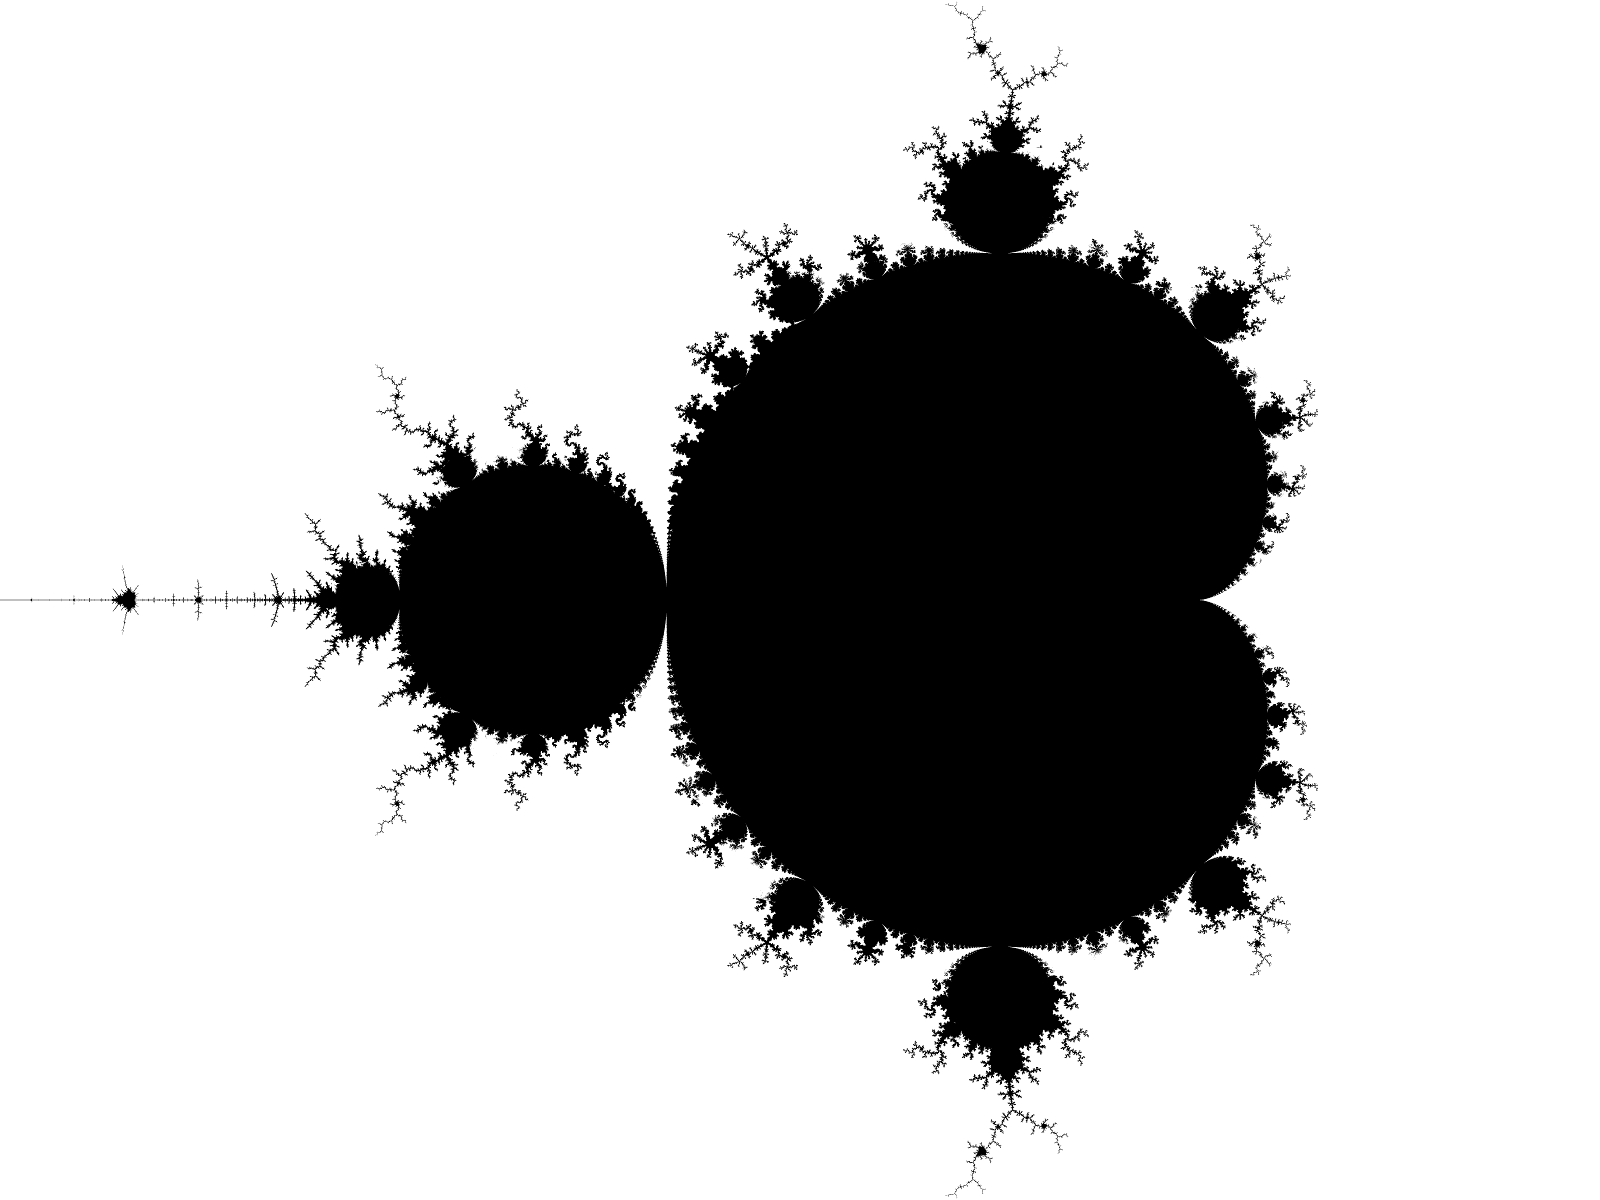
\includegraphics[width=\textwidth]{mandelbrot.png}
\end{center}
\caption{L'insieme di Mandelbrot generato al computer. Si veda il
codice a pagina \pageref{code:Mandelbrot}.}
\label{fig:mandelbrot}
\end{figure}

E' molto complicato determinare il carattere delle successioni definite
dal sistema~\eqref{eq:mandelbrot}.
Solo con l'utilizzo dei primi calcolatori
Mandelbrot (1924-2010) riuscì a rappresentare graficamente
\mymargin{insieme!di Mandelbrot}%
\index{Mandelbrot!insieme di}
l'insieme $M$ dei punti $c\in \CC$ per i quali la successione $z_n$ non diverge:
si veda la figura~\ref{fig:mandelbrot}.

Con l'esercizio~\ref{ex:mandelbrot_reale}
abbiamo trovato l'intersezione $M\cap \RR = [-2,1/4]$.
Nel seguente esercizio ci proponiamo ora di dimostrare un'altra semplice
proprietà che può essere
molto utile negli algoritmi numerici utilizzati per disegnare tale insieme.

\begin{exercise}[raggio di fuga]
Dimostrare che se $z_n$ è soluzione di \eqref{eq:mandelbrot}
se per un qualche $N\in \NN$ si ha $\abs{z_N}> 2$ allora $\abs{z_n}\to +\infty$
per $n\to +\infty$. In particolare l'insieme $M$ di Mandelbrot
è contenuto nel disco $\ENCLOSE{z\in \CC \colon \abs{z}\le 2}$.
\end{exercise}
%
\begin{proof}{Soluzione.}
Sia $c\in \CC$ fissato e si $z_n$ la successione definita da~\eqref{eq:mandelbrot}.
Per ogni $\eps>0$ consideriamo l'insieme:
\[
  A_\eps = \ENCLOSE{z \in \CC \colon \abs{z}\ge c \text{ e } \abs{z}\ge 2+\eps}.
\]
Possiamo mostrare che l'insieme $A_\eps$ è invariante in quanto se $z_n\in A_\eps$
si ha
\begin{equation}\label{eq:473244}
\begin{aligned}
\abs{z_{n+1}}
&= \abs{z_n^2+c}
\ge \abs{z_n}^2 - \abs{c}
\ge \abs{z_n}^2 - \abs{z_n}
= (\abs{z_n}-1)\abs{z_n}\\
&\ge (1+\eps)\abs{z_n}
\ge (1+\eps)(2+\eps)
\ge 2+\eps.
\end{aligned}
\end{equation}
Dunque $A_\eps$ è invariante ma non solo, se $z_n \in A_\eps$ abbiamo
trovato che risulta $\abs{z_{n+1}} \ge (1+\eps) \abs{z_n}$
e dunque $\abs{z_{n+k}} \ge (1+\eps)^k \abs{z_n}$ e dunque
$\abs{z_n}\to +\infty$ per $n\to +\infty$.

Se $\abs{c}\le 2$ e se $\abs{z_N}> 2$ allora $z_N \in A_\eps$ per
un qualche $\eps>0$ e dunque possiamo concludere che
$z_n\to \infty\in \bar \CC$.
Se invece $\abs{c}>2$ è facile osservare che $z_0 = 0$, $z_1=c$, $z_2=c^2+c$
e quindi
\[
  \abs{z_2}
    = \abs{c^2+c}
    \ge \abs{c}^2 - \abs{c}
    = \abs{c}(\abs{c}-1)
    \ge \abs{c} > 2
\]
dunque $z_2 \in A_\eps$ e quindi, comunque, $z_n\to \infty$.

\end{proof}


\chapter{equazioni differenziali}
\label{ch:edo}

\section{classificazione}

Le equazioni differenziali sono una classe di \emph{equazioni funzionali}
\mynote{equazioni funzionali}
\index{equazione!funzionale}
ovvero
equazioni in cui l'incognita non è un numero (come accade nelle equazioni algebriche) ma è una funzione. La funzione incognita $u$, sarà quindi funzione di una variabile indipendente $u=u(x)$.
Ad esempio $u$ potrebbe essere la traiettoria di un proiettile che descrive la posizione nello spazio in funzione del tempo $x$. Se nelle equazioni algebriche il nome di gran lunga più utilizzato per l'incognita è $x$, nelle equazioni funzionali a seconda dei contesti le convenzioni possono cambiare in maniera drastica. Si dovrà utilizzare un nome per la funzione e un nome per la sua variabile indipendente: $x=x(t)$, $y=y(x)$, $y=y(t)$, $u=u(x)$ sono alcune delle scelte più utilizzate.
Se l'incognita è una funzione $u=u(x)$ le operazioni che possono comparire nell'equazioni sono,
oltre le usuali operazioni algebriche che agiscono sui singoli valori $u(x)$ della funzione,
anche operatori che agiscono sulla funzione $u$ in sé.
Se l'equazione funzionale oltre alle operazioni algebriche comprende anche
l'operatore derivata, si dirà che è una \mynote{equazione differenziale}%
\index{equazione!differenziale}
\emph{equazione differenziale}.
Di contro ci potranno ad esempio essere equazioni che coinvolgono l'operatore integrale e si chiameranno
\emph{equazioni integrali}.

Ci sono quindi diversi concetti che possono aiutare a classificare le equazioni differenziali.
Innanzitutto supporremo sempre che le nostre equazioni siano \myemph{senza ritardo}
(o \emph{senza memoria})
cioè che la funzione $u$ e le sue derivate $u'$, $u''$\dots,
vengano tutte calcolate nello stesso punto $x$.
In caso contrario si parla di
equazioni \emph{differenziali funzionali} (in particolare \emph{equazioni con ritardo}
perché le derivate dipendono tipicamente dai valori assunti nel passato),
argomento che non toccheremo.

Se la funzione incognita è funzione di una singola variabile si dirà che l'equazione è una
\emph{equazione differenziale ordinaria}
\mynote{ODE}%
\index{equazione!differenziale!ordinaria}%
(abbreviato
\emph{EDO} \index{EDO}%
in italiano,
\emph{ODE} \index{ODE}%
per gli anglosassoni).
Di contro se la funzione incognita è funzione di più variabili l'equazione si chiamerà
\emph{equazione differenziale alle derivate parziali}
\mynote{PDE}%
\index{equazione!differenziale!alle derivate parziali}%
 (abbreviato \emph{EDP} \index{EDP} in italiano e \emph{PDE}
 \index{PDE} in lingua inglese).
In questo corso, centrato sulle funzioni di una variabile, tratteremo quindi solamente le equazioni differenziali ordinarie.
L'\emph{ordine}
\mynote{ordine}%
\index{ordine!equazione differenziale}%
\index{equazione!differenziale!ordine}%
dell'equazione differenziale è il numero massimo di derivate successive che vengono applicate alla funzione incognita.
La funzione $u$ sarà definita su un intervallo $I$ della retta reale: $u\colon I \to \RR$
e la funzione e le derivate vengono tutte valutate nello stesso punto. In tal caso
la forma più generale di equazione differenziale ordinaria di ordine $n$ si potrà dunque scrivere come:
\begin{equation}\label{eq:3784643}
  F(x,u(x),u'(x),u''(x), \dots, u^{(n)}(x)) = 0
\end{equation}
con $F\colon \Omega \to \RR$ una funzione data, definita su un insieme $\Omega \subset I\times \RR^{n+1}$.
Una funzione $u\colon I \to \RR$ si dice essere una \emph{soluzione
dell'equazione differenziale} \eqref{eq:3784643} se $u$ è derivabile almeno
$n$ volte in ogni punto $x\in I$ e se \eqref{eq:3784643} è soddisfatta
per ogni $x\in I$.

Usualmente si tende a semplificare la notazione evitando di scrivere sempre
esplicitamente il punto $x$ in cui viene calcolata la funzione.
Sarà quindi usuale
scrivere l'equazione \eqref{eq:3784643}
nella forma abbreviata:
\[
  F(x,u,u',u'', \dots, u^{(n)}) = 0
\]
rendendo anche più evidente il fatto che l'incognita è $u$,
l'intera funzione, e non un singolo valore $u(x)$.


Se ad esempio scegliamo $n=2$ e $F(x,u,v,z)= z+\sin u + v$ otteniamo l'equazione differenziale:
\begin{equation}\label{eq:39872}
 u''(x) + \sin u(x) + u'(x) = 0
\end{equation}
che, in opportune unità di misura, è l'equazione del moto di un pendolo smorzato,
dove $x$ rappresenta il tempo e $u$ la misura dell'angolo di inclinazione del
pendolo rispetto alla verticale.
Osserviamo che nell'esempio precedente la funzione $F$ non dipende direttamente
dalla variabile $x$. Equazioni con questa proprietà si dicono
\emph{equazioni autonome}
\mynote{equazioni autonome}
\index{equazione!differenziale!autonoma}
ed è immediato osservare che se $u(x)$ è soluzione anche una sua traslazione
temporale $v(x) = u(x-x_0)$ è soluzione dell'equazione
(il moto del pendolo non dipende dall'ora in cui si svolge).

Una equazione scritta nella forma \eqref{eq:3784643} si dice \emph{equazione in forma implicita}
\mynote{equazione in forma implicita}%
\index{equazione!differenziale!in forma implicita}%
e per analogia con le equazioni algebriche (si pensi all'equazione
$u^2(x) + x^2 = 1$) ci si aspetta che le soluzioni di tale equazioni siano
meglio rappresentate da curve piuttosto che da grafici di funzione.
Risulta in effetti che la teoria delle equazioni differenziali si applica con
molta maggiore efficacia alle \emph{equazioni in forma normale}
\mynote{equazioni in forma normale}
\index{equazione!differenziale!in forma normale}
che sono le equazioni differenziali di ordine $n$ che possono essere scritte
esplicitando la dipendenza dalla derivata di ordine massimo:
\begin{equation}\label{eq:366793}
 u^{(n)}(x) = f(x, u(x), u'(x), \dots, u^{n-1}(x))
\end{equation}
dove $f\colon \Omega \to \RR$ è una funzione definita su $\Omega\subset I\times \RR^n$.
L'equazione del pendolo si può scrivere in questa forma,
scegliendo $f(x,u,v) = -\sin u - v$.

Più in generale potremmo considerare
\emph{sistemi di equazioni differenziali}
\mynote{sistemi}%
\index{sistemi di equazioni differenziali}%
\index{equazione!differenziale!sistema}%
in più incognite.
Possiamo rappresentare un sistema di $k$ equazioni ordinarie in $m$ incognite nella forma:
\begin{equation}\label{eq:375456}
  \vec F(x, \vec u(x), \vec u'(x), \dots, \vec u^{n}(x)) = \vec 0
\end{equation}
dove $\vec u$ è una funzione $\vec u \colon I \to \RR^m$ le cui componenti sono
le $m$ funzioni incognite:
\[
  \vec u(x) = (u_1(x), \dots, u_m(x))
\]
mentre la funzione $\vec F \colon I \times (\RR^m)^{n+1} \to \RR^k$ è stavolta
una funzione a valori vettoriali $\vec F = (F_1, \dots, F_k)$ cosicché l'equazione vettoriale
\eqref{eq:375456} è effettivamente equivalente ad un sistema di $k$ equazioni:
\[
\begin{cases}
F_1(x,\vec u(x), \vec u'(x)\dots, \vec u^{(n)}(x)) = 0\\
F_2(x,\vec u(x), \vec u'(x)\dots, \vec u^{(n)}(x)) = 0\\
\quad\vdots \\
F_k(x,\vec u(x), \vec u'(x)\dots, \vec u^{(n)}(x)) = 0\\
\end{cases}
\]
Vedremo che per le equazioni ordinarie del primo ordine è naturale,
come accade per le equazioni algebriche,
avere lo stesso numero di equazioni e di incognite dunque è tipico avere singole
equazioni scalari del primo ordine
(cioè in cui l'incognita è una funzione a valori nel campo
degli scalari $\RR$)
o sistemi di $k=m$ equazioni del primo ordine con incognita una funzione
vettoriale $\vec u$ (cioè una funzione a valori nello spazio vettoriale $\RR^m$)
ovvero con $m$ incognite $u_1,\dots, u_m$ funzioni scalari.

Una importante osservazione è il fatto generale che una equazione differenziale
di ordine $n$ può essere ricondotta ad un sistema di $n$ equazioni
differenziali del primo ordine.
Basta infatti considerare come incognita il vettore (chiamato \emph{jet})
\[
  \vec u = (u, u', u'', \dots, u^{(n-1)})
\]
comprendente tutte le derivate della funzione scalare $u$ fino all'ordine $n-1$.
L'equazione \eqref{eq:3784643}, di ordine $n$, risulta infatti equivalente
al sistema di $n$ equazioni del primo ordine nella variabile
$\vec u = (u_1, \dots, u_n)$
\[
  \begin{cases}
    u_2(x) = u_1'(x)\\
    u_3(x) = u_2'(x)\\
    \quad \vdots \\
    u_{n}(x) = u_{n-1}'(x)\\
    F(x, u_1(x), u_2(x), \dots, u_n(x), u_n'(x)) = 0
  \end{cases}
\]
Nel caso, più interessante,
delle equazioni in forma normale
l'equazione~\eqref{eq:366793} di ordine $n$
diventa un sistema di $n$ equazioni normali
del primo ordine
in $n$ incognite
\[
  \begin{cases}
  u_1'(x) = u_2(x)\\
  u_2'(x) = u_3(x)\\
  \quad \vdots\\
  u_{n-1}'(x) = u_n(x)\\
  u_n'(x) = f(x,u_1(x), u_2(x), \dots, u_n(x))
  \end{cases}
\]
ovvero una equazione differenziale vettoriale
del primo ordine
\[
  \vec u'(x) = \vec f(x, \vec u(x)).
\]
\begin{comment}
avendo definito $\vec f = (f_1, \dots, f_n)$
come
\begin{gather*}
  f_1(x, y_1,\dots, y_n) = y_2 \\
  f_1(x, y_1,\dots, y_n) = y_3 \\
  \quad \vdots \\
  f_{n-1}(x, y_1,\dots, y_n) = y_n \\
  f_n(x, y_1,\dots, y_n) = f(x,y_1, \dots, y_n)
\end{gather*}
\end{comment}

Nell'esempio del pendolo \eqref{eq:39872} si avrà come incognita una funzione vettoriale
$\vec u(x) = (u(x),u'(x))$ le cui componenti sono posizione e velocità angolare.
Il codominio di tale funzione si chiama \emph{spazio delle fasi}.
L'equazione (essendo autonoma tralasciamo la dipendenza da $x$)
si scriverà nella forma $\vec u' = \vec f(\vec u)$ con
$\vec f(y_1,y_2) = (y_2, -\sin(y_1) - y_2)$.

Un caso molto particolare ma decisamente importante è quello in cui la funzione
$F$ (per le equazioni in forma implicita) o la funzione $f$
(per le equazioni in forma normale) sono funzioni lineari
per ogni $t$
rispetto alla variabile $u$.
In tal caso diremo che l'equazione è
\mynote{equazioni lineari omogenee}%
\index{equazione!differenziale!lineare omogenea}%
\emph{lineare omogenea}.
Più precisamente si avrà
\[
F(x,u(x),u'(x), \dots, u^{(n)}(x)) = A_x(u(x), u'(x), \dots, u^{(n)}(x))
\]
con $A_x\colon \RR^{n+1}\to \RR$
operatore lineare per ogni $x$ ovvero $A_x$ si rappresenta tramite un vettore
i cui coefficienti sono funzioni della variabile $x$:
\[
  A_x(\vec y) = \sum_{k=0}^n a_k(x) y_k
\]
e l'equazione differenziale si scrive nella forma
\[
  a_0(x) u(x) + a_1(x) u'(x) + \dots + a_n(x) u^{(n)}(x) = 0.
\]
Nel caso in cui i coefficienti $a_k(t)$ non dipendano da $x$
(cioè siano funzioni costanti) diremo che l'equazione è
lineare
\mynote{coefficienti costanti}%
\index{equazione!differenziale!lineare a coefficienti costanti}%
\emph{a coefficienti costanti}.

E' facile osservare che l'insieme delle soluzioni di una equazione lineare omogenea è uno spazio vettoriale: $u=0$ è sempre soluzione, se $u$ è una soluzione e $\lambda \in \RR$ anche $\lambda u$ è soluzione e se $u$ e $v$ sono due soluzioni anche $u+v$ è soluzione
\mymargin{principio di sovrapposizione}
\index{principio di sovrapposizione}
(principio di sovrapposizione).

In effetti
se le funzioni $u$ sono definite su un intervallo $I$ possiamo
identificare $F$ con un funzionale $L\colon \RR^I \to \RR^I$ definito da
\[
  L(u)(x) = F(x,u(x), u'(x), \dots, u^{(n)}(x))
\]
Se l'equazione differenziale è lineare allora $L$ è un operatore lineare
sullo spazio vettoriale $\RR^I$ e lo spazio delle soluzioni dell'equazione
differenziale non è altro che $\ker L$, il nucleo dell'operatore,
ed è noto che $\ker L$ è un sottospazio vettoriale.
Nonostante $\RR^I$ sia uno spazio vettoriale di dimensione infinita scopriremo
che (sotto opportune ipotesi) lo spazio vettoriale delle soluzioni
ha dimensione finita $n$, uguale al grado dell'equazione.

Nel caso in cui la funzione $F$ (o la corrispondente $f$)
sia affine si dirà che l'equazione differenziale
è una equazione
\mynote{equazione lineari}%
\index{equazione!differenziale!lineare}%
\emph{lineare (non omogenea)}.
L'equazione non omogenea avrà la forma:
\[
  a_0(x) u(x) + a_1(x) u'(x) + \dots + a_n(x) u^{(n)}(x) = g(x).
\]
Se $v_0$ e $v_1$ sono due soluzioni di questa equazione è chiaro che la
differenza $u=v_1 - v_0$ è soluzione dell'equazione omogenea
\[
  a_0(x) u(x) + a_1(x) u'(x) + \dots + a_n(x) u^{(n)}(x) = 0.
\]
Dunque quest'ultima si chiama equazione omogenea associata alla non omogenea
e se $v_0$ è una soluzione particolare (qualunque) dell'equazione non omogenea
ogni soluzione $v$ dell'equazione non omogenea si scrive nella forma
\[
  v = v_0 + u
\]
con $u$ soluzione dell'omogenea associata.
Per trovare tutte le soluzioni di una equazione non omogenea è dunque
sufficiente trovare una soluzione particolare e tutte le soluzioni della
equazione omogenea associata.

L'equazione del pendolo \eqref{eq:39872} non è lineare
ma quando l'angolo $u$ è piccolo (cioè per \emph{piccole oscillazioni}) si ha $\sin u \sim u$.
Facendo questa \emph{linearizzazione} si ottiene l'equazione
\[
  u''(x)  + u(x) + u'(x) = 0.
\]
Questa è una equazione lineare omogenea.
Se sul pendolo agisce una forza esterna (pendolo forzato) l'equazione diventa
\[
  u''(x) + u(x) + u'(x) = g(x)
\]
dove $g(x)$ rappresenta l'entità di una forza esterna variabile nel tempo.
Questa equazione è lineare non omogenea.

Come nel caso generale le equazioni lineari di ordine $n$ si riconducono
a sistemi lineari di $n$ equazioni del primo ordine.

Se le equazioni differenziali di ordine $n$ hanno uno spazio di
soluzioni di
dimensione $n$ ci si aspetta che qualcosa del genere succeda anche
per le equazioni differenziali di ordine $n$ in forma normale.
Lo spazio delle soluzioni non sarà lineare ma, in un certo senso,
avrà comunque dimensione $n$ cioè le soluzioni potranno essere identificate
da $n$ parametri.
Per fare questo ad una equazione differenziale in forma normale
di ordine $n$
\[
u^{(n)}(x) = f(x, u(x), \dots, u^{n-1}(x))
\]
si aggiunge una \myemph{condizione iniziale} ovvero si fissa un
\emph{punto iniziale} $x_0$ e un \emph{valore iniziale}
per ognuna delle derivate di ordine inferiore a $n$:
$u(x_0) = y_0$, $u'(x_0)=y_1$, \dots, $u^{n-1}(x_0) = y_{n-1}$.
Questa condizione
si chiama \emph{condizione di Cauchy} e il problema
che si ottiene mettendo una condizione di Cauchy ad una
equazione differenziale:
\[
  \begin{cases}
  u^{(n)}(x) = f(x, u(x), \dots, u^{n-1}(x))\\
  u(x_0) = y_0, \\
  u'(x_0) = y_1, \\
  \vdots\\
  u^{(n-1)}(x_0) = y_{n-1}
  \end{cases}
\]
si chiama \myemph{problema di Cauchy}.
Vedremo che, sotto opportune ipotesi, il problema di Cauchy
ammette una unica soluzione e questo significa, sostanzialmente,
che l'insieme di tutte le soluzioni dell'equazione differenziale
può essere descritto dal variare
degli $n$ parametri $y_0, y_1, \dots, y_{n-1}$.

Una delle ipotesi fondamentali per garantire l'unicità delle
soluzioni di un problema di Cauchy è che le soluzioni siano
definite su un intervallo. E' chiaro infatti che se ho due
soluzioni definite su due intervalli separati, potrei unire
le due soluzioni e ottenere una soluzione definita sull'unione dei
due intervalli. Viceversa una soluzione definita
su un intervallo $I$ è soluzione anche se ristretta ad ogni sottoinsieme
di $I$ (che sia o no un intervallo).
Se restringo una soluzione o unisco due soluzioni ottengo formalmente
soluzioni diverse in quanto i domini di definizione sono diversi, ma
queste soluzioni assumono, dove sono definite, gli stessi valori.
Per evitare questa ambiguità considereremo sempre solamente
le soluzioni definite su un \myemph{intervallo massimale} cioè
soluzioni definite su un intervallo che non possono essere
estese su intervalli più grandi.


\section{metodi risolutivi}

Una tipologia di equazioni differenziali che abbiamo già trattato
è data dalle equazioni della forma:
\[
   u'(x) = f(x).
\]
Banalmente l'insieme delle soluzioni è dato dalle primitive di $f$:
\[
  u \in \int f.
\]
Se $f$ è definita su un intervallo tutte le soluzioni $u$ definite sullo stesso
intervallo e, grazie al Teorema~\ref{th:primitive}
si scrivono quindi nella forma
\[
  u(x) = F(x) + c
\]
dove $F$ è una qualunque primitiva di $f$ e $c\in \RR$ è una costante additiva
arbitraria.
Se $f$ è continua e consideriamo il problema di Cauchy:
\[
  \begin{cases}
    u'(x) = f(x) \\
    u(x_0) = y_0.
  \end{cases}
\]
possiamo identificare una unica soluzione
che si scrive nella forma:
\[
  u(x) = y_0 + \int_{x_0}^x f(t)\, dt.
\]

\subsection{equazioni lineari del primo ordine}

Le equazioni differenziali ordinarie del primo
ordine in forma normale possono essere scritte nella forma:
\mymark{***}
\begin{equation}\label{eq:47744}
   u'(x) + a(x) u(x) = b(x).
\end{equation}

Per risolvere queste equazioni si cerca di ricondurre la somma
nel lato sinistro alla derivata di un prodotto.
Per fare ciò si considera una qualunque primitiva
$A\in \int a$ e si moltiplicano ambo i membri
per $e^{A(x)}$:
\[
  e^{A(x)} u'(x) + a(x) e^{A(x)} u(x) = b(x) e^{A(x)}
\]
essendo $A'(x) = a(x)$
si osserva che il lato sinistro è ora la derivata di un prodotto:
\[
  \enclose{e^{A(x)}u(x)}' = b(x) e^{A(x)}
\]
da cui
\[
  e^{A(x)} u(x) \in \int b(x) e^{A(x)}\, dx.
\]
Moltiplicando ambo i membri per $e^{-A(x)}$ (visto che l'esponenziale
non si annulla mai questa operazione non modifica lo spazio delle soluzioni)
si ottiene
\[
u(x) = e^{-A(x)} \int b(x) e^{A(x)}\, dx, \qquad
A(x) \in \int a(x)\, dx.
\]

Più esplicitamente
scelta una qualunque primitiva del lato destro
\[
  F(x) \in \int b(x) e^{A(x)}\, dx
\]
su ogni intervallo in cui $a(x)$ e $b(x)$ sono definite
si ha
\[
  u(x) = e^{-A(x)}\enclose{F(x) + c}.
\]
per qualche $c\in \RR$.

Se $b(x)=0$ l'equazione è lineare omogenea, possiamo scegliere $F(x) = 0$
e quindi lo spazio delle soluzioni in questo caso
è dato da
\[
  u(x) = c e^{-A(x)}
\]
ed è quindi lo spazio vettoriale unidimensionale generato dalla funzione $e^{-A(x)}$.

Ogni soluzione della equazione non omogenea si può scrivere come somma di una
soluzione particolare $u_0$ della equazione non omogenea
più una generica soluzione dell'equazione omogenea associata. Infatti:
\[
  u(x) = u_0(x) + c e^{-A(x)}
\]
dove
\[
  u_0(x) = e^{-A(x)}F(x)
\]
è una particolare soluzione dell'equazione non omogenea.

Osserviamo che se $a(x)$ e $b(x)$ sono funzioni continue definite su uno stesso
intervallo $I$, anche la soluzione è definita su tutto $I$.
Si dirà quindi che la soluzione esiste \emph{globalmente}.

\begin{exercise}[autovettori dell'operatore derivata]
Fissato $\lambda \in \RR$ trovare tutte le soluzioni dell'equazione
\[
  u'(x) = \lambda u(x).
\]
\end{exercise}
%
\begin{proof}[Svolgimento]
Scriviamo l'equazione nella forma
\[
  u'(x) - \lambda u(x) = 0.
\]
Nelle notazioni precedenti abbiamo $a(x) = -\lambda$ e quindi possiamo scegliere $A(x) = -\lambda x \in \int a$.
Moltiplicando ambo i membri per $e^{-A(x)}$ si ottiene
\[
  e^{-\lambda x} u'(x) - \lambda e^{-\lambda x} u(x) = 0
\]
cioè
\[
 \enclose{e^{-\lambda x}\cdot u(x)}' = 0
\]
da cui su ogni intervallo in cui $u$ è definita esiste una costante $c$ tale che
\[
  e^{-\lambda x} u(x) = c
\]
ovvero
\[
  u(x) = c e^{\lambda x}.
\]
Abbiamo dunque trovato che le soluzioni sono definite su tutto $\RR$, una soluzione è $e^{\lambda x}$ e ogni altra soluzione è multiplo di questa.
\end{proof}

\begin{exercise}
\begin{enumerate}
\item
Trovare le soluzioni dell'equazione differenziale
\[
  u' - \frac{u}{x} = x^2.
\]

\item
Trovare le soluzioni dell'equazione differenziale
\[
  x u' - u = x^3.
\]
\end{enumerate}
\end{exercise}
\begin{proof}[Svolgimento]
La prima è una equazione lineare non omogenea del primo ordine
del tipo~\eqref{eq:47744}. Il fattore integrante è $e^{A(x)}$ con
\[
  A(x) \in \int a(x)\, dx = -\int \frac{1}{x}\, dx \ni - \ln \abs{x}.
\]
Dunque $e^{A(x)} = 1/\abs{x}$. Dovremmo dunque dividere ambo i membri dell'equazione per $\abs{x}$. Osserviamo che l'equazione non è definita per $x=0$ e possiamo dunque distinguere i casi $x>0$ e $x<0$. Decidiamo quindi, per semplicità, di cambiare segno all'equazione per $x<0$ cosicché possiamo dividere per $x$ invece che per $\abs{x}$.
Si ottiene dunque:
\[
  \frac{u'}{x} - \frac{u}{x^2} = x
\]
cioè
\[
  \enclose{u\cdot \frac{1}{x}}'  = x
\]
da cui
\[
  \frac{u}{x} \in \int x\, dx \ni \frac{x^2}{2}.
\]
Dunque la funzione $u(x)/x$ differisce da $x^2/2$ per una costante su ognuno dei due intervalli $x>0$ e $x<0$. Su ognuno dei due intervalli si ha dunque:
\[
  \frac{u(x)}{x} = \frac{x^2}{2} + c
\]
da cui
\[
  u(x) = \frac{x^3}{2} + c x
\]
per qualche $c\in \RR$. Per come è stato posto il problema, la soluzione non deve essere definita per $x=0$ e la costante $c$ può essere quindi diversa se $x>0$ o $x<0$.

La seconda equazione è equivalente alla prima se $x\neq 0$. Ma non è in forma normale e le soluzioni
potranno essere definite anche per $x=0$.
Si avrà quindi
\[
  u(x) = \frac{x^3}{2} + c x
\]
come prima ma affinché la funzione sia derivabile in $x=0$ la costante $c$ dovrà essere uguale per $x>0$ e per $x<0$.

Si osservi che ogni soluzione soddisfa la condizione iniziale $u(0) = 0$ e che quindi nessuna soluzione soddisfa la condizione $u(0)= q$ se $q \neq 0$.
\end{proof}

\begin{exercise}
Risolvere l'equazione differenziale:
\[
 u' + \frac{u}{(1+x^2)\arctg x} = 1.
\]
\end{exercise}
%
\begin{proof}[Svolgimento.]
Osserviamo che l'equazione è definita solo per $x\neq 0$. Cercheremo quindi le soluzioni sui due intervalli $x<0$ e $x>0$.
Moltiplicando ambo i membri dell'equazione per $\arctg x$ si ottiene
\[
  \arctg x \cdot u'(x) +\frac{1}{1+x^2} u(x) = \arctg x
\]
cioè:
\[
  \enclose{\arctg x \cdot u(x)}' = \arctg x
\]
da cui
\[
  \arctg x \cdot u(x) \in \int \arctg x\, dx \ni x \arctg x - \frac {1}{2}\ln(1+x^2).
\]
Dunque su ogni intervallo su cui la soluzione è definita esisterà
$c\in \RR$ tale che
\[
  \arctg x \cdot u(x) = x \arctg x - \frac{1}{2}\ln(1+x^2) + c
\]
da cui essendo $x\neq 0$ si può dividere per $\arctg x$ e ottenere
\[
  u(x) = x - \frac{\ln(1+x^2)}{2\arctg x} + \frac{c}{\arctg x}.
\]
Abbiamo quindi una famiglia di soluzioni definite per $x<0$ e una famiglia di soluzioni definite per $x>0$.
\end{proof}

\subsection{equazioni a variabili separabili}

Si chiamano equazioni a variabili separabili le
equazioni del tipo:
\mymark{***}
\begin{equation}\label{eq:edo_separabile}
  u'(x) = f(x) \cdot g(u(x)).
\end{equation}
Questa è una equazione del primo ordine in forma normale:
\[
  u'(x) = F(x, u(x))
\]
dove nella funzione $F$ risulta possibile separare le
due variabili in un prodotto:
\[
  F(x, y) = f(x)\cdot g(y).
\]

Se $u$ è una soluzione dell'equazione~\eqref{eq:edo_separabile}
e se $x$ è un punto in cui $g(u(x))\neq 0$, possiamo dividere ambo i membri dell'equazione per $g(u(x))$ per ottenere:
\[
  \frac{u'(x)}{g(u(x))} = f(x).
\]
Vogliamo ora scrivere il lato sinistro come la derivata della funzione composta. Se scegliamo una primitiva di $1/g$:
\[
  H(u) \in \int \frac{1}{g(u)}\, du
\]
si osserva che
\[
  \enclose{H(u(x))}' = H'(u(x))\cdot u'(x) = \frac{u'(x)}{g(u(x))} = f(x).
\]
dunque se $F\in \int f$, su ogni intervallo in cui $g(u(x))\neq 0$ dovrà esistere $c\in \RR$ tale che
\[
  H(u(x)) = F(x) + c.
\]
Se supponiamo inoltre che $H$ sia invertibile si avrà:
\[
  u(x) = H^{-1}(F(x)+ c).
\]

\begin{example}
Risolviamo l'equazione
\begin{equation}\label{eq:43856}
  u' = x u^2 + x.
\end{equation}
E' una equazione del primo ordine in forma normale.
Raccogliendo $x$ al lato destro si ottiene una equazione a variabili separabili.
Dividendo ambo i membri per $u^2+1$ (che è sempre diverso da zero) si ottiene l'equazione equivalente
\[
\frac{u'}{1+u^2} = x.
\]
Integrando il lato sinistro si ottiene:
\[
  \int \frac{u'(x)}{1+u^2(x)}\, dx
  = \Enclose{\int \frac{du}{1+u^2}}_{u=u(x)}
  \ni \arctg(u(x))
\]
mentre per il lato destro si ottiene
\[
  \int x\, dx \ni \frac{x^2}{2}.
\]
Dunque su ogni intervallo si deve avere
\[
  \arctg(u(x)) = \frac{x^2}{2} + c.
\]
Visto che l'arcotangente assume valori compresi tra $-\pi/2$ e $\pi/2$ anche il lato destro dovrà rimanere in tale intervallo. Dovrà quindi essere:
\begin{equation}\label{eq:4856}
  -\frac \pi 2 < \frac {x^2} 2 + c < \frac \pi 2 .
\end{equation}
Con questa condizione possiamo invertire l'arcotangente ottenendo finalmente una espressione per la soluzione:
\begin{equation}\label{eq:45876314}
  u(x) = \tg\enclose{\frac{x^2}{2} + c}.
\end{equation}

\begin{figure}
\myurl{43856}{i grafici delle soluzioni dell'equazione differenziale (\getrefnumber{eq:43856})}
\centering
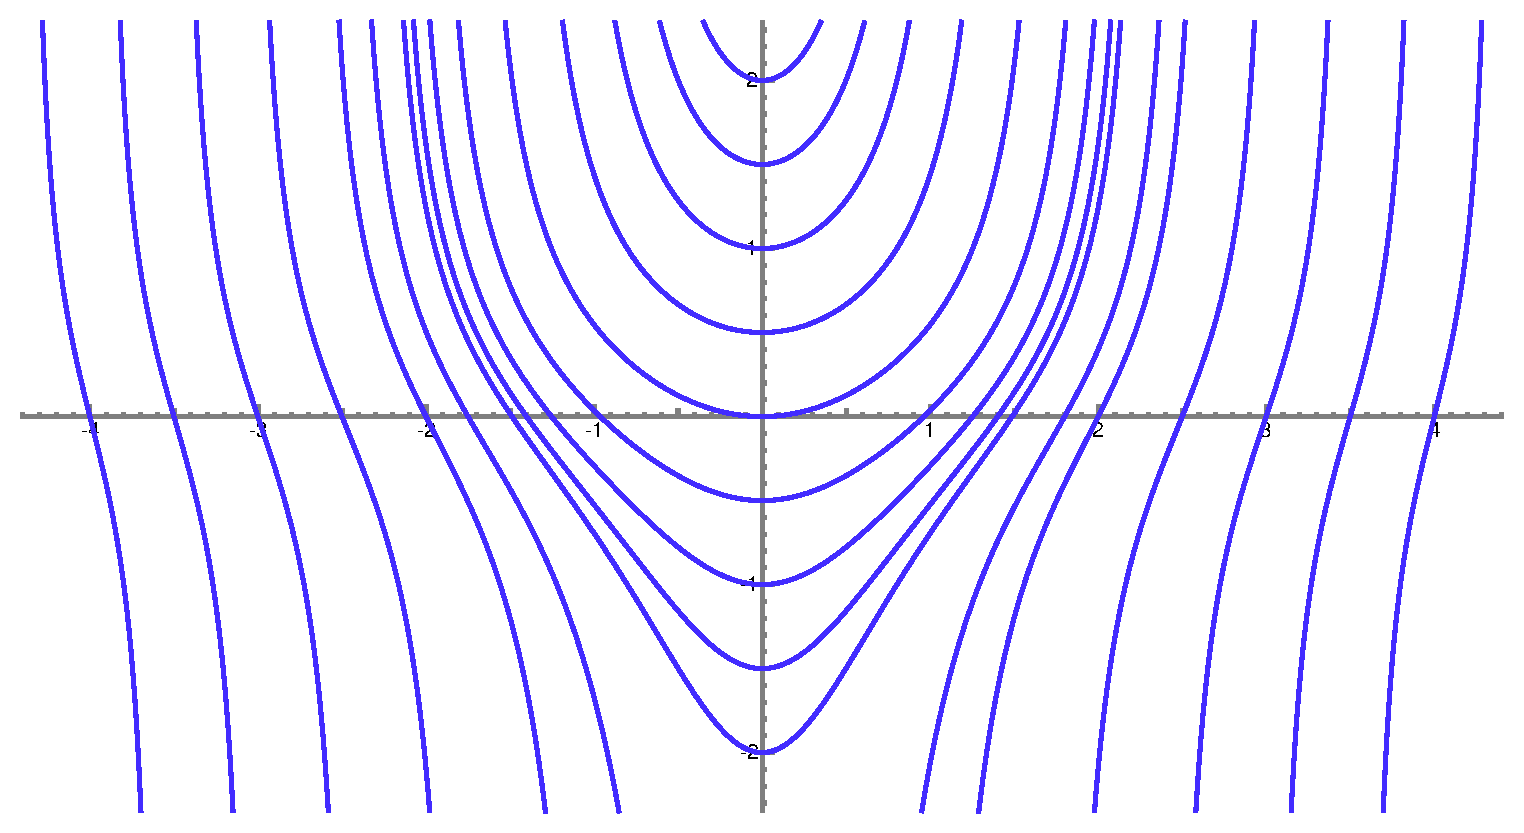
\includegraphics[width=0.8\textwidth]{fig_43856.pdf}
\label{fig:43856}
\caption{i grafici delle soluzioni dell'equazione differenziale~\eqref{eq:43856}.-}
\end{figure}

Osserviamo che la condizione~\eqref{eq:4856} equivale a richiedere che l'argomento
della tangente stia nell'intervallo $\enclose{-\frac \pi 2, \frac \pi 2}$.
In tal caso dovrà essere $c<\frac\pi 2$ e si osserva che se $c>-\frac \pi 2$
la soluzione $u(x)$ è definita su un intervallo aperto centrato in $x=0$ mentre
se $c \le -\frac \pi 2$ la soluzione è definita su una coppia di intervalli
simmetrici con ampiezza che tende a zero quando $c\to -\infty$.
Agli estremi di tali intervalli la soluzione ha degli asintoti verticali.

In questo caso possiamo osservare che la condizione~\eqref{eq:4856} può essere
trascurata, visto che la funzione $\tg$ è $\pi$-periodica e quindi
è possibile sommare a $c$ un multiplo intero di $\pi$ senza che la soluzione
venga modificata.
Nell'equazione~\eqref{eq:45876314} si potrebbe
quindi considerare la funzione $\tg$
definita su tutto il suo dominio osservando che in tal caso si può
supporre che sia $c\in \left(-\frac \pi 2, \frac \pi 2\right]$.
Invece di ottenere un singolo intervallo per ogni $c$ si ottengono così
tutti gli infiniti intervalli.
\end{example}

\begin{remark}
L'esempio precedente mette in evidenza il fatto che le soluzioni massimali possono essere definite
su intervalli arbitrariamente piccoli anche se l'equazione differenziale
non presenta singolarità. Diremo in questo caso che
la soluzione non è globale.
\end{remark}

\begin{example}
Si voglia risolvere l'equazione
\[
  u' = u^2.
\]
Si tratta di una equazione in forma normale, del primo ordine, autonoma.
In particolare è a variabili separabili
$u' = f(u(x))\cdot g(x)$
con $f(u)=u^2$ e $g(x)=1$.
Osserviamo innanzitutto che $u(x) = 0$ è soluzione in quanto $u'(x) = u^2(x) = 0$.
Se $u$ è una soluzione non identicamente nulla ci saranno dei punti in cui
$u(x)\neq 0$.
In un intorno di tali punti possiamo dividere ambo i membri dell'equazione per $u^2(x)$ ottenendo:
\[
  \frac{u'}{u^2} = 1.
\]
Integrando il lato sinistro tramite cambio di variabile $u=u(x)$, $du=u'(x)\, dx$ si ottiene:
\[
  \int \frac{u'(x)}{u^2(x)}\, dx = \Enclose{\int \frac{du}{u^2}}_{u=u(x)} = \Enclose{-\frac{1}{u}}_{u=u(x)}
  = -\frac{1}{u(x)}
\]
mentre integrando il lato destro si ha
\[
  \int 1 \, dx \ni x.
\]
Dunque su ogni intervallo in cui $u(x)\neq 0$ deve esistere una costante $c\in \RR$ tale che
\[
-\frac{1}{u(x)} = x + c
\]
ovvero, ponendo $x_0 = -c$
\begin{equation}\label{eq:5782196}
  u(x) = -\frac{1}{x+c} = \frac{1}{x_0-x}.
\end{equation}

In conclusione abbiamo trovato una soluzione costante $u(x)=0$ e una famiglia
di soluzioni definite sugli intervalli $(-\infty,x_0)$ e $(x_0,+\infty)$
rappresentante dall'equazione~\eqref{eq:5782196}.
Dovremmo ora chiederci
se è possibile che queste soluzioni vengano mescolate tra loro, ovvero
se una soluzione può valere zero in alcune zone e soddisfare~\eqref{eq:5782196}
in altre.

In questo caso la risposta è no.
Basta osservare che una funzione $u$ che soddisfa l'equazione~\eqref{eq:5782196}
può tendere a zero solamente quando $x\to +\infty$ o $x\to -\infty$.
Questo significa che se consideriamo una soluzione $u(x)$
definita su un intervallo $I$ e se in almeno un punto la soluzione è diversa da zero,
allora la soluzione è diversa da zero su tutto $I$ e
soddisfa l'equazione~\eqref{eq:5782196} in quanto la soluzione nulla e la
soluzione \eqref{eq:5782196} non sono tra loro compatibili (non possono essere
incollate con continuità).

Vedremo più avanti un risultato
(proposizione~\ref{prop:separazione_soluzioni})
che garantisce in ipotesi molto generali (che sono soddisfatte per questa
equazione) due diverse soluzioni non
possono mai incontrarsi.
\end{example}

\begin{exercise}
Fissato $p>1$ si risolva l'equazione differenziale
\[
  u' = u^p
\]
e si osservi che la soluzione presenta sempre un asintoto verticale
(dunque non c'è esistenza globale).
\end{exercise}

\begin{example}[baffo di Peano]
Si determinino tutte le soluzioni del problema di Cauchy
\begin{equation}
\label{eq:94467}
\begin{cases}
  u'(x) = \sqrt[3]{u(x)}\\
  u(0)=0
\end{cases}
\end{equation}
\end{example}
%
\begin{figure}
\myurl{94467}{Il baffo di Peano formato dalle soluzioni del problema di Cauchy (\getrefnumber{eq:94467})}
\centering
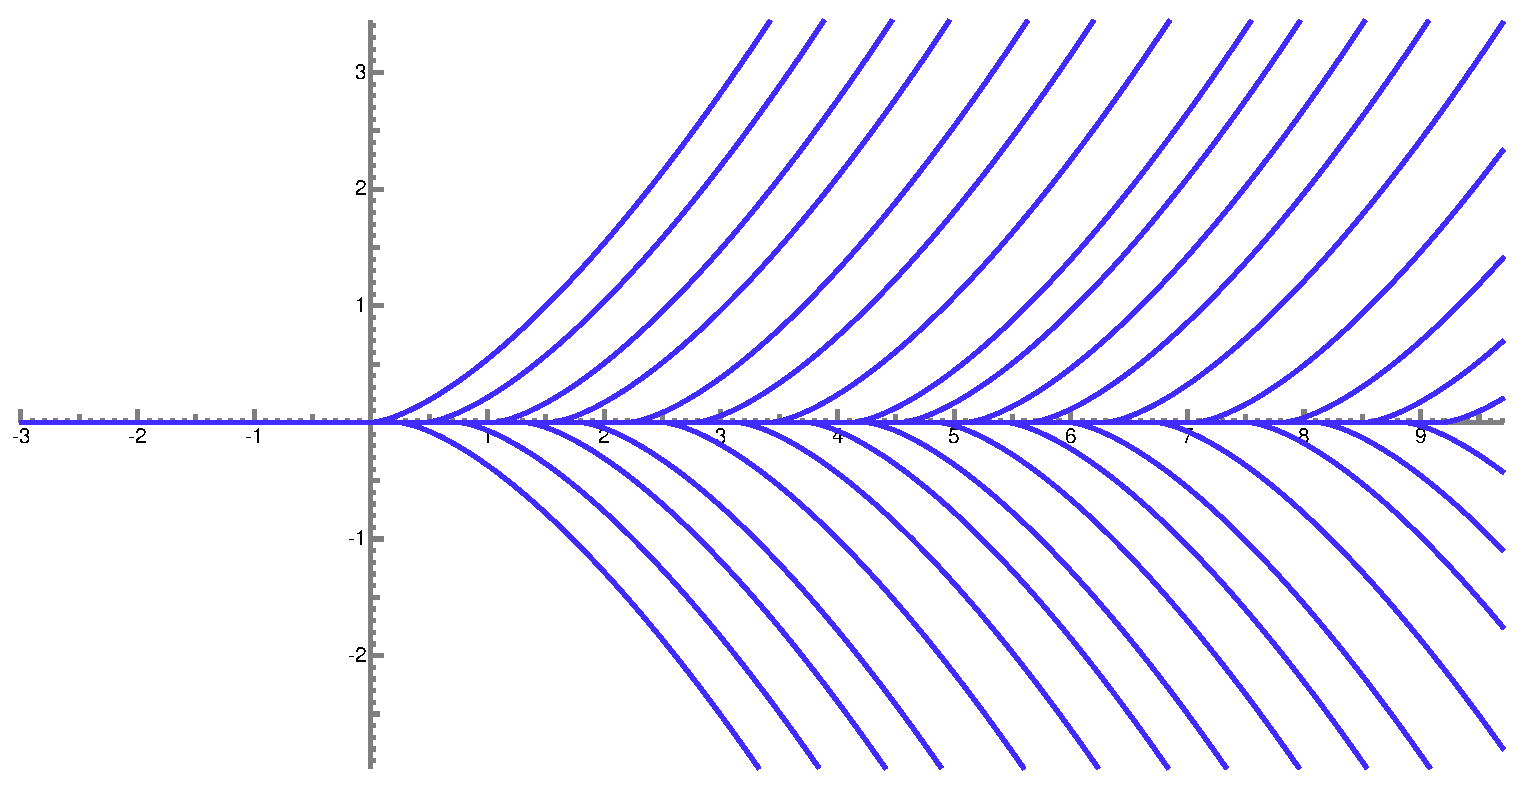
\includegraphics[width=0.9\textwidth]{fig_94467.pdf}
\label{fig:94467}
\caption{Il baffo di Peano formato dalle soluzioni del problema di Cauchy~\eqref{eq:94467}.}
\end{figure}
%
\begin{proof}[Svolgimento.]
Osserviamo che la funzione nulla $u(x)=0$ è soluzione dell'equazione
e soddisfa la condizione $u(0)=0$.
Ma a priori non possiamo escludere che ci siano altre soluzioni dell'equazione
che verifichino la stessa condizione (vedremo che la
proposizione~\ref{prop:separazione_soluzioni} non si applica in questo caso
particolare).

Nei punti in cui $u(x)\neq 0$ possiamo riscrivere l'equazione nella forma
\[
  \frac{u'(x)}{\sqrt[3]{u(x)}} = 1.
\]
Integrando il lato sinistro tramite il cambio di variabili $u=u(x)$,
$du = u'(x)\, dx$,
si ottiene
\[
  \int \frac{u'(x)}{\sqrt[3]{u(x)}}\, dx
  = \Enclose{\int \frac{du}{\sqrt[3]u}}_{u=u(x)}
  \ni \frac 3 2 \sqrt[3]{u^2(x)}.
\]
integrando anche il lato destro troviamo dunque
che su ogni intervallo su cui $u$ è definita e $u(x)\neq 0$
deve esistere una costante $c$ tale che
\[
  \frac 3 2 \sqrt[3]{u^2(x)} = x + c.
\]
Risolvendo in $u(x)$:
\begin{equation}\label{eq:476937568}
  u(x) = \pm \sqrt{\enclose{\frac 2 3 (x+c)}^3}.
\end{equation}
Osserviamo che la proprietà precedente
può essere soddisfatta solamente se $x\ge -c$ ma affinché
sia $u(x)\neq 0$ dobbiamo imporre $x>-c$.
Ma per $x\to -c^+$
si ha $u(x)\to 0$ e anche $u'(x) = \sqrt[3]{u(x)}\to 0$.
Significa che una soluzione definita su $x>c$ mediante
la~\eqref{eq:476937568} può essere estesa a tutto $\RR$
ponendo $u(x)=0$ per $x\le c$.
Affinché valga la condizione $u(0)=0$ sarà dunque sufficiente
imporre la restrizione $-c\ge 0$.

Il nostro problema ha dunque infinite soluzioni definite
su tutto $\RR$. Per la precisione, per ogni $c\ge 0$
(cambiamo segno alla costante trovata prima, in modo che risulti
positiva)
si hanno le soluzioni
\[
  u(x) = \begin{cases}
    0 & \text{per $x\le c$}\\
    \sqrt{\enclose{\frac 2 3 (x-c)}^3} & \text{per $x>c$}
  \end{cases}
\]
e
\[
  u(x) = \begin{cases}
    0 & \text{per $x\le c$}\\
    -\sqrt{\enclose{\frac 2 3 (x-c)}^3} & \text{per $x>c$}
  \end{cases}
\]
\end{proof}
\subsection{altri metodi risolutivi}

Nella sezione precedente abbiamo visto che le equazioni lineari del primo ordine
e le equazioni
a variabili separabili possono essere ricondotte al calcolo di una primitiva.
Nella sezione~\ref{sec:edo_lineari} verranno esposti i metodi risolutivi per le
equazioni lineari di ordine $n$ a coefficienti costanti.

Ci sono molti altri tipi di equazioni che possono essere ricondotti
alle equazioni lineari o alle equazioni a variabili separabili.
Non potremo dilungarci su questi metodi ma può essere utile,
come riferimento non esaustivo,
un elenco di alcune tipologie di equazioni per le quali esiste un metodo
risoluvtivo:

\begin{enumerate}
\item \emph{equazione del secondo ordine senza dipendenza da $u$}
\[
  F(x, u', u'') = 0
\]
si riconduce al primo ordine ponendo $v(x)=u'(x)$;
\item \emph{equazione del secondo ordine autonoma}
\[
  F(u, u', u'') = 0
\]
si riconduce al primo ordine
ponendo $v(u(x)) = u'(x)$;
\item \emph{equazione di Bernoulli}
\[
  u' = a(x) u + b(z) u^\alpha
\]
si riconduce ad una equazione lineare ponendo
$v(x) = u(x)^{1-\alpha}$;
\item \emph{equazione di Clairaut}
\[
  u = x u' + f(u');
\]
la derivata dell'equazione si fattorizza: un
fattore dà soluzioni della forma $u(x)=mx+q$ l'altro fattore diventa
una equazione algebrica facendo la sostituzione $u(x) = v(u'(x))$;
\item \emph{equazione di Riccati}
\[
  u' = u^2 + b(x) u + c(x).
\]
si ponga $u'(x) = -v'(x)/v(x)$ per ricondursi ad
una equazione lineare del secondo ordine in $v$;
\end{enumerate}

\begin{example}[equazione di Newton]
Un sistema fisico unidimensionale soggetto a forze che dipendono solamente
dalla posizione può essere descritto da un problema di Cauchy:
\[
\begin{cases}
  u''(x) = F(u(x)) \\
  u(x_0) = u_0 \\
  u'(x_0) = v_0
\end{cases}
\]
(ad esempio per il pendolo si ha $F(y) = -\sin y$).
La funzione $v$ definita da $v(u(x)) = u'(x)$ mette in relazione
la velocità con la posizione e descrive quindi il moto nel
cosiddetto \emph{spazio delle fasi}. Con tale sostituzione si
trova
\[
  u''(x) = v'(u(x)) u'(x) = v'(u(x)) v(u(x))
\]
che sostituita in $u'' = F(u)$ ci dà una equazione
differenziale del primo ordine per $v=v(u)$:
\[
 v' v  = F(u).
\]
Questa è una equazione del primo ordine a variabili separabili
che può essere interpretata come la legge di conservazione dell'energia,
infatti è equivalente a
\[
  \frac{d}{dx}\enclose{\frac 1 2 v^2 - \int F(u)} = 0
\]
dove $\frac 1 2 v^2$ si interpreta come energia cinetica e $-\int F$
come energia potenziale.
Integrando tra $x_0$ e $x$ e utilizzando le condizioni iniziali si ottiene,
con $u=u(x)$:
\[
  \frac 1 2 v^2(u) = \frac 1 2 v_0^2 + \int_{u_0}^{u} F(y)\, dy.
\]
Questa equazione descrive la traiettoria del sistema nel piano delle fasi $(u,v)$
e ci permette di ricavare $v$ in funzione di $u$:
\[
  v(u) = \pm\sqrt{v_0^2 + 2\int_{u_0}^u F(u)\, du}
\]
che significa:
\begin{equation}\label{eq:8844475}
  u'(x) = \pm \sqrt{v_0^2 + 2 \int_{u_0}^{u(x)} F(y)\, dy}.
\end{equation}
Questa è una equazione autonoma in $u$, quindi a variabili separabili:
\[
  \pm\frac{u'(x)}{\sqrt{v_0^2 - \int_{u_0}^{u(x)} F(y)\, dy}} = 1
\]
che può essere integrata tra $x_0$ e $x$ facendo il cambio di variabile $u=u(x)$
\[
  \pm\int_{u_0}^{u(x)} \frac{du}{\sqrt{v_0^2-\int_{u_0}^u F(y)\, dy}} = x-x_0.
\]
In questo modo abbiamo determinato la funzione inversa della soluzione $u(x)$.
\end{example}

\begin{example}[periodo del pendolo]
Sia $u(x)$
l'angolo di scostamento dalla verticale
al tempo $x$ di un pendolo semplice di lunghezza $\ell$.
Considerando la componente tangenziale della accelerazione di gravità
(il cui modulo è $g$)
l'equazione di Newton può essere scritta nella forma:
\[
  u''(x) = -\frac{g}{\ell} \sin u(x).
\]
Siamo quindi nel caso dell'esempio precedente dove $F(u) = -\frac{g}{\ell} \sin u$
e se al tempo $x=0$ lasciamo cadere da fermo il pendolo da un angolo $u_0$,
si avrà $v_0=0$. L'energia potenziale sarà data allora da
\[
-\frac{g}{\ell}\int_{u_0}^u \sin y\, dy = \frac{g}{\ell}\enclose{\cos u - \cos u_0}.
\]
L'equazione~\eqref{eq:8844475} diventa dunque
\[
  u'(x) = \pm \sqrt{2\frac{g}{\ell}(\cos u(x) - \cos u_0)}.
\]
Separando le variabili e integrando tra $0$ e $x$ si ottiene
\[
\sqrt{\frac \ell g}\int_0^x \frac{u'(t)\, dt}{\pm\sqrt{2\cos u(t)-2\cos u_0}}
= \int_0^x dt  = x.
\]
Cambiando variabile $u=u(x)$, $du = u'(x) dx$:
\begin{equation}\label{eq:4898944}
\sqrt{\frac \ell g}\int_0^{u(x)} \frac{du}{\pm\sqrt{2\cos u-2\cos u_0}} = x.
\end{equation}
La scelta del segno $\pm$ è arbitraria ma visto che $u$ è continua
anche $u'=-\sin u$ deve essere una funzione continua. Dunque il segno
$\pm$ può cambiare solo quando $u'=0$. Nel punto iniziale $x=0$ abbiamo
imposto $u'(0) = 0$ e dunque l'energia cinetica è nulla. Visto che l'energia
cinetica non può essere negativa significa che l'energia potenziale
non può aumentare e quindi inizialmente l'angolo $u(x)$ dovrà diminuire
(o almeno: non potrà aumentare). Dunque inizialmente il segno di $u'$ è negativo
e rimarrà negativo finché non si avrà nuovamente $u'(x)=0$.
L'integrale in~\eqref{eq:4898944} è un integrale improprio in quanto
la funzione integranda presenta un asintoto per $u\to u_0^-$ dobbiamo dunque
assicurarci che l'integrale sia finito. Sviluppando $\cos u$ nel punto $u=u_0$
si trova $\cos u = \cos u_0  - \sin u_0 \cdot (u-u_0) + o(u-u_0)$ da cui
\[
 \frac{1}{\sqrt{2 \cos u - 2 \cos u_0}}
 =\frac{1}{\sqrt{2\sin u_0\cdot (u_0-u) + o(u-u_0)}}
 \sim \frac{C}{\sqrt{u_0-u}}
\]
che è notoriamente una funzione integrabile per $u\to u_0^-$.

Vogliamo ora calcolare il tempo $x_1$ in cui il pendolo raggiunge per la prima
volta la verticale, cioè $u(x_1)=0$.
Ricordiamo che al tempo $x=0$ il pendolo parte da un angolo $u_0$
con velocità nulla. Nell'intervallo $x\in[0,x_1]$ si avrà $u'(x)<0$
(l'angolo diminuisce) dunque:
\[
-\sqrt{\frac{\ell}{g}}\int_{u_0}^{0} \frac{du}{\sqrt{2\cos u - 2\cos u_0}}
= x_1.
\]

Una volta raggiunta la verticale, per simmetria il pendolo tornerà a risalire
fino ad un angolo $-u_0$ mettendoci lo stesso tempo $x_1$. Poi tornerà a scendere
e risalire fino a tornare all'angolo $u_0$ mettendoci in totale un tempo
$T=4x_1$ che è quindi il periodo di oscillazione. Si ha dunque
\[
  \frac{T}{4} = \sqrt{\frac \ell g}\int_0^{u_0} \frac{du}{\sqrt{2\cos u - 2\cos u_0}}.
\]

Purtroppo l'integrale che abbiamo trovato non ha una primitiva
esprimibile mediante funzioni elementari (è un integrale ellittico).
Il nostro obiettivo è ora quello di farne uno sviluppo di Taylor
per $u_0\to 0$ che significa determinare
il periodo del pendolo per \myemph{piccole oscillazioni}.

Tramite formule di bisezione possiamo scrivere $\cos u = 1 - 2 \sin^2\frac u 2$
da cui
\[
 \sqrt{2\cos u - 2\cos u_0}
 = \sqrt{4\sin^2 \frac {u_0} 2 - 4 \sin^2 \frac{u}{2}}
 = 2\sin u_0 \sqrt{1-\enclose{\frac{\sin \frac u 2}{\sin \frac {u_0}2}}^2}
\]
dunque ponendo
\begin{equation}\label{eq:4847843}
 \sin t = \frac{\sin \frac u 2}{\sin \frac{u_0} 2}
\end{equation}
si ha
\[
  \sqrt{\frac \ell g} \cdot \frac T 4
  =  \int_0^{u_0} \frac{du}{2\sin \frac {u_0}2 \sqrt{1-\sin^2 t}}
  = \int_0^{u_0} \frac{du}{2\sin \frac{u_0}2 \cos t}
\]
ma per il cambio di variabile~\eqref{eq:4847843} si ha
\[
  \cos t \, dt = \frac{\cos \frac u 2 }{2 \sin \frac{u_0} 2}\, du
\]
ovvero
\[
 \frac{du}{2\sin \frac {u_0} 2 \cos t} = \frac{dt}{\cos \frac u 2}
 = \frac{dt}{\sqrt{1-\sin^2 t \sin^2\frac{u_0}{2}}}
\]
e quindi
\[
\sqrt{\frac g \ell} \cdot \frac{T}{4}
= \int_0^{\frac \pi 2} \frac{dt}{\cos \frac u 2}
= \int_0^{\frac \pi 2} \frac{dt}{\sqrt{1-\sin^2 \frac u 2}}
= \int_0^{\frac \pi 2} \frac{dt}{\sqrt{1-\sin^2 \frac{u_0}{2} \sin^2 t}}.
\]
Utilizzando ora la serie binomiale (teorema~\ref{th:serie_binomiale})
possiamo scrivere
\begin{align*}
\sqrt{\frac g \ell} \cdot\frac{T}{4}
&= \int_0^{\frac \pi 2} \sum_{k=0}^{+\infty}{-\frac 1 2 \choose k} \enclose{-\sin^2 t\sin^2 \frac{u_0}2}^{k}\, dt.\\
&= \int_0^{\frac \pi 2} \sum_{k=0}^{+\infty}\frac{(2k-1)!!}{(2k)!!} \enclose{\sin^2 t\sin^2 \frac{u_0}2}^{k}\, dt.
\end{align*}
in quanto si ha
\begin{align*}
  {-\frac 1 2 \choose k}
  &= \frac{\enclose{-\frac 1 2}\cdot \enclose{-\frac 3 2} \cdots \enclose{-\frac{2k-1} 2}}{k!}\\
  &= (-1)^k\frac{(2k-1)!!}{2^k \cdot k!} = (-1)^k \frac{(2k-1)!!}{(2k)!!}.
\end{align*}
Rispetto alla variabile $\sin^2 t$ dentro all'integrale abbiamo ora una serie di potenze
con coefficienti
\[
 a_k = \frac{(2k-1)!!}{(2k)!!} \enclose{\sin^2\frac{u_0} 2}^{k}
\]
e si verifica facilmente che
$  \frac{a_{k+1}}{a_k} \to \sin^2 \frac{u_0}{2}$
dunque la serie di potenze converge se
$ \sin^2 t \le \frac{1}{\sin^2 \frac{u_0}{2}}$
che significa semplicemente
$ \sin \frac u 2 < 1$.
Stiamo quindi facendo un integrale esteso all'intero raggio
di convergenza della serie. Sappiamo che la serie
converge totalmente e quindi uniformemente sugli intervalli
chiusi strettamente contenuti nel raggio di convergenza.
Visto che la serie è a termini positivi le somme parziali
convergono alla somma della serie e sono tutte inferiori
a tale somma.
Abbiamo già visto, inoltre, che la somma della serie
è integrabile con integrale finito.
Dunque possiamo applicare
il teorema di convergenza dominata (teorema~\ref{th:convergenza_dominata} con $f=g$)
per scambiare la serie con l'integrale:
\[
\sqrt{\frac g \ell} \cdot\frac{T}{4}
= \sum_{k=0}^{+\infty}\frac{(2k-1)!!}{(2k)!!} \enclose{\sin \frac{u_0}2}^{2k}
\int_0^{\frac \pi 2}  \enclose{\sin t}^{2k}\, dt
\]
l'integrale è ora sostanzialmente lo stesso $I_n$ che abbiamo calcolato nel teorema~\ref{th:wallis}:
\[
  \int_0^{\frac \pi 2} \enclose{\sin t}^{2k}\, dt
  = \frac 1 2 \int_0^{\pi} \enclose{\sin t}^{2k}\, dt
  = \frac{I_{2k}}{2}
  = \frac \pi 2 \cdot\frac{(2k-1)!!}{(2k)!!}
\]
da cui
\[
T
= 2\pi\sqrt{\frac \ell g}\sum_{k=0}^{+\infty} \enclose{\frac{(2k-1)!!}{(2k)!}}^2
\enclose{\sin \frac{u_0} 2}^{2k}.
\]

Possiamo allora cercare di scrivere i primi termini dello sviluppo di
Taylor di $T = T(u_0)$ per $u_0\to 0$ diciamo, per esempio, fino all'ordine 8
in $u_0$. Basterà considerare la somma dei termini della
serie per $k=0,1,2,3,4$ in quanto la somma dei termini per $k\ge 5$ mi darà
 un contributo dell'ordine di $O\enclose{\sin \frac {u_0} 2}^{10} = o(u_0^8)$. Dunque
 \begin{align*}
 \sqrt{\frac{g}{\ell}}\cdot \frac{T}{2\pi}
 &=
 1 + \enclose{\frac 1 2}^2 \sin^2 \frac{u_0} 2
 + \enclose{\frac{1\cdot 3}{2\cdot 4}}^2\enclose{\sin^2 \frac {u_0} 2}^2 \\
 &\quad + \enclose{\frac{1\cdot 3 \cdot 5}{2\cdot 4 \cdot 6}}^2
 \enclose{\sin^2 \frac {u_0} 2}^3 + \enclose{\frac{1\cdot 3\cdot 5 \cdot 7}{2\cdot 4\cdot 6\cdot 8}}^2
 \enclose{\sin^2 \frac {u_0} 2}^4 + o(u_0^8) \\
% \end{align*}
% \begin{align*}
 %
 &=
1 + \frac 1 4 \enclose{\frac{u_0^2}{4} - \frac{u_0^4}{2^4\cdot 3} + \frac{u_0^6}{2^5\cdot 3^2\cdot 5}
- \frac{u_0^8}{2^8\cdot 3^2\cdot 5\cdot 7}} \\
&\quad + \frac{3^2}{2^6}\enclose{\frac{u_0^2}{4} - \frac{u_0^4}{2^4\cdot 3}
+ \frac{u_0^6}{2^5\cdot 3^2\cdot 5}}^2\\
&\quad + \frac{5^2}{2^8}\enclose{\frac{u_0^2}{4} - \frac{u_0^4}{2^4\cdot 3}}^3
+ \frac{5^2\cdot 7^2}{2^{14}}
\frac {u_0^8} {2^8} + o(u_0^8)\\
%
%\end{align*}
%\begin{align*}
&=
1 + \frac{u_0^2}{2^4} - \frac{u_0^4}{2^6\cdot 3} + \frac{u_0^6}{2^7\cdot 3^2\cdot 5}
- \frac{u_0^8}{2^{10}\cdot 3^2\cdot 5\cdot 7} \\
&\quad + \frac{3^2}{2^6}\enclose{\frac{u_0^4}{2^4} - \frac{u_0^6}{2^5\cdot 3} + \frac{u_0^8}{2^8\cdot 3^2} + \frac{u_0^8}{2^6\cdot 3^2\cdot 5}}\\
&\quad + \frac{5^2}{2^8}\enclose{\frac{u_0^6}{2^6} - \frac{u_0^8}{2^8}}
+ \frac{5^2\cdot 7^2}{2^{22}}
u_0^8 + o(u_0^8)\\
%
% \end{align*}
% \begin{align*}
&= 1 + \frac{u_0^2}{2^4} + \frac{11}{2^{10}\cdot 3} u_0^4
 + \frac{173}{2^{14}\cdot 3^2\cdot 5} u_0^6
 + \frac{22931}{2^{22}\cdot 3^2\cdot 5\cdot 7} u_0^8
 + o(u_0^8).\\
\end{align*}

\end{example}

%%%%%%%%%%%%%%%%%%%%
%%%%%%%%%%%%%%%%%%%%
%%%%%%%%%%%%%%%%%%%%
\section[funzioni vettoriali e di più variabili]{alcuni risultati preparatori
sulle funzioni vettoriali e di più variabili}
%%%%%%%%%%%%%%%%%%%%
%%%%%%%%%%%%%%%%%%%%
%%%%%%%%%%%%%%%%%%%%

Ci sarà utile estendere la definizione delle classi di regolarità $C^k$ alle
funzioni vettoriali (cioè con codominio $\RR^n$) e di più variabili
(cioè con dominio $\RR^m$).

Se $\Omega\subset \RR^m$ è un insieme aperto e $f\colon \Omega \to \RR$
è una funzione, vogliamo definire le \emph{derivate parziali} di $f$.
Se $\vec x \in \Omega$ si ha $\vec x = (x_1,\dots, x_m)$ e quindi
$f(\vec x) = f(x_1,\dots, x_m)$. Se facciamo variare una sola componente
$x_j$ mantenendo fisse tutte le altre componenti, otteniamo una funzione
di una variabile $x_j \mapsto g(x_j) = f(x_1,\dots, x_j, \dots, x_m)$.
Definiamo dunque la \emph{derivata parziale}
\mynote{derivata parziale}
\index{derivata!parziale}
di $f$ rispetto alla variabile $x_j$ come la derivata della funzione $g(x_j)$.
Denotiamo tale derivata con il simbolo:
\[
  \frac{\partial f}{\partial x_j}.
\]
Le derivate parziali si calcolano dunque come le usuali derivate per le
funzioni di una variabile, solamente bisogna considerare costanti tutte
le variabili tranne quella coinvolta nella derivazione.
Ad esempio se $f(x,v) = -\sin(x) - v$
(come nell'esempio fatto nell'introduzione) si ha
\begin{align*}
  \frac{\partial f}{\partial x} &= -\cos(x)\\
  \frac{\partial f}{\partial v} &= -1.
\end{align*}

Se $\vec f\colon \Omega \subset \RR^m \to \RR^n$ è una funzione di più
variabili a valori vettoriali potremo scrivere $\vec f = (f_1, \dots, f_n)$
e considerare le derivate parziali di ogni componente:
\[
  \frac{\partial \vec f}{\partial x_j}
  = \enclose{\frac{\partial f_1}{\partial x_j}, \dots, \frac{\partial f_n}{\partial x_j}}.
\]

\begin{definition}
Sia $\Omega\subset \RR^m$ un aperto. Denoteremo con $C^0(\Omega,\RR^n)$
lo spazio vettoriale di tutte le funzioni
continue $f\colon \Omega \to \RR^n$.

Denotiamo con $C^1(\Omega,\RR^n)$ lo spazio vettoriale
delle funzioni in $C^0(\Omega,\RR^n)$ tali che ognuna delle loro derivate
parziali $\frac{\partial f}{\partial x_j}$ esiste in ogni punto di $\Omega$ ed
è a sua volta una funzione continua (cioè in $C^0(\Omega,\RR^n)$).
Ricorsivamente si definisce $C^k(\Omega,\RR^n)$ per $k>1$,
come lo spazio delle funzioni $\Omega\to\RR^n$ tali che tutte le loro derivate
parziali stanno in $C^{k-1}(\Omega,\RR^n)$.

Quando lo spazio di arrivo non è indicato si sottointende sempre $\RR$, quindi
$C^k(\Omega) = C^k(\Omega,\RR)$.
\end{definition}

\begin{theorem}[stabilità delle funzioni regolari]
Sia $\Omega \subset \RR^n$ un aperto.
Se $f,g\in C^k(\Omega)$ allora anche $f+g$, $f-g$, $f\cdot g$ e $\frac{f}{g}$
(dove è definita) sono di classe $C^k$. Se $f\in C^k(\Omega)$ e $g\in C^k(\RR)$
allora $g\circ f \in C^k(\Omega)$.
\end{theorem}
%
\begin{proof}
Il fatto che la composizione di funzioni continue sia una funzione continua
è vero in generale in qualunque spazio metrico.
Infatti se $f\colon X\to Y$ e $g\colon Y \to Z$ e se $x_k\to x$ in $X$
allora $f(x_k) \to f(x)$ in $Y$ (per la continuità di $f$)
e quindi $g(f(x_k)) \to g(f(x))$ in $Z$ (per la continuità di $g$).
Dunque $(g \circ f)(x_k) \to (g\circ f)(x)$ e $g\circ f\colon X\to Z$ è continua.

Possiamo dunque osservare che le funzioni di due variabili $s(x,y) = x+y$,
$d(x,y)=x-y$ e
$m(x,y)=xy$ sono funzioni continue da $\RR^2\to \RR$ 
(grazie ai teoremi~\ref{th:limite_somma} e \ref{th:limite_prodotto}). 
Questo garantisce
che la somma, la differenza e il prodotto di funzioni continue siano funzioni continue.
Anche il reciproco di funzioni continue è una funzione continua
in quanto la funzione $r(x)=1/x$ è continua.
Ne consegue che il rapporto di funzioni continue è una
funzione continua.

Veniamo ora alle derivate parziali.
Per le regole di derivazione delle funzioni di una variabile sappiamo che
somma, prodotto, differenza, rapporto (ove definito) e composizione
di funzioni derivabili sono
a loro volta funzioni derivabili e la derivata si esprime sempre mediante
somma, prodotto, differenza e rapporto delle funzioni coinvolte e delle loro
derivate. Dunque quello che si ottiene combinando tra loro funzioni
di classe $C^k$ è una funzione continua le cui derivate parziali esistono e
sono di classe $C^{k-1}$, dunque è una funzione di classe $C^k$.
\end{proof}


\begin{definition}
Sia $\vec f\colon [a,b]\to \RR^m$, $\vec f(x) = (f_1(x), \dots, f_m(x))$.
Diremo che $\vec f$ è integrabile su $[a,b]$ se ogni
$f_k\colon[a,b]\to \RR$ è integrabile su $[a,b]$ e in tal caso porremo:
\[
  \int_a^b \vec f(x)\, dx
  = \enclose{\int_a^b f_1(x)\, dx, \dots, \int_a^b f_m(x)\, dx}
  \in \RR^m
\]
cosicché per ogni $k=1,\dots, m$ si ha:
\[
  \enclose{\int_a^b \vec f(x)\, dx}_k = \int_a^b f_k(x)\, dx.
\]
Come al solito si pone inoltre $\int_b^a \vec f = - \int_a^b \vec f$.
\end{definition}

\begin{theorem}\label{teo:tipo_jensen}
\mymark{*}
Sia $\vec f\colon [a,b]\to \RR^m$ integrabile. Allora si ha
\[
  \abs{\int_a^b \vec f(x)\, dx} \le \int_a^b \abs{\vec f(x)}\, dx.
\]
\end{theorem}
%
\begin{proof}
Posto
\[
 \vec v = \int_a^b \vec f(x)\, dx
\]
si ha, usando la linearità dell'integrale
e sfruttando la disuguaglianza di Cauchy-Schwarz
\begin{align*}
  \abs{\vec v}^2
  &= \vec v \cdot \vec v
   = \sum_{k=1}^n v_k \int_a^b f_k(x)\, dx
   = \int_a^b \sum_{k=1}^m v_k f_k(x)\, dx \\
  &= \int_a^b \enclose{\vec v, \vec f(x)}\, dx
  \le \int_a^b \abs{\vec v}\cdot \abs{\vec f(x)}\, dx
  = \abs{\vec v} \int_a^b \abs{\vec f(x)}\, dx.
\end{align*}
Se $\abs{\vec v}\neq 0$ possiamo dividere ambo i membri per $\abs{\vec v}$ e
ottenere la disuguaglianza cercata.
Altrimenti se $\abs{\vec v}=0$ la disuguaglianza è certamente soddisfatta in
quanto il lato destro non può essere negativo.
\end{proof}


%%%%%
%%%%%
%%%%%
%%%%%
\section{Il problema di Cauchy}
%%%%%
%%%%%
%%%%%
%%%%%

Il problema di Cauchy
per i sistemi del primo ordine
consiste nel
trovare una soluzione di un sistema di $n$ equazioni differenziali ordinarie del primo ordine in $n$ incognite
con un dato iniziale fissato. Cioè dato $x_0\in \RR$,
e $\vec y_0 \in \RR^n$ si cerca un intervallo $I\subset \RR$ con $x_0\in I$ e una funzione $\vec u \colon I\to \RR^n$
che sia derivabile e che soddisfi:
\begin{equation}\label{eq:problema_cauchy}
\begin{cases}
 \vec u'(x) = \vec f(x, \vec u(x)), \qquad \forall x\in I\\
 \vec u(x_0) = \vec y_0.
\end{cases}
\end{equation}

\begin{definition}[Cauchy-Lipschitz]
\label{def:cauchy_lipschitz}
Diremo che una funzione $\vec f\colon \Omega\subset \RR\times \RR^n \to \RR^m$
soddisfa la \myemph{proprietà di Cauchy-Lipschitz} se $f$ è continua e se
per ogni $(x_0,\vec y_0)\in \Omega$ esiste un intorno $U$ di $(x_0,\vec y_0)$
ed esiste $L\ge 0$
tale che se $(x,\vec y_1)\in U$ e $(x,\vec y_2)\in U$ si ha
\[
  \abs{\vec f(x,\vec y_1)- \vec f(x,\vec y_2)} \le L \abs{\vec y_1- \vec y_2}
\]
A parole potremmo dire: $\vec f(x,\vec y)$ è localmente lipschitziana rispetto
a $\vec y$ uniformemente
rispetto a $x$.
\end{definition}

\begin{theorem}[Cauchy-Lipschitz, esistenza e unicità locale]
\label{th:cauchy_lipschitz}%
\mymargin{esistenza e unicità locale per i sistemi del primo ordine}%
\mymark{***}%
Sia $\Omega$ un aperto di $\RR\times \RR^n$ e sia $\vec f\colon \Omega \to \RR^n$,
una funzione con la proprietà di Cauchy-Lipschitz
(definizione~\ref{def:cauchy_lipschitz}).

Allora dato $(x_0,\vec y_0)\in \Omega$
esiste $\delta>0$
tale che preso qualunque intervallo $I\subset [x_0-\delta,x_0+\delta]$
con $x_0\in I$
esiste una unica funzione $\vec u\colon I \to \RR^n$
tale che $(x,\vec u(x))\in \Omega$ per ogni $x\in I$
che soddisfa il problema di Cauchy~\eqref{eq:problema_cauchy}.
\end{theorem}
%
%
\begin{proof}
\mymark{***}
L'idea della dimostrazione è che integrando ambo i lati dell'equazione
$\vec u' = f(x,\vec u)$ e tenendo conto della condizione iniziale, si
ottiene una equazione del tipo $\vec u = T(\vec u)$ dove $T$ è un operatore
sullo spazio delle funzioni continue.
Scegliendo $\delta$ abbastanza piccolo si riuscirà a mostrare che le funzioni
definite su un intervallo di raggio $\delta$ intorno a $x_0$ risultano
essere uno spazio invariante per $T$ e, eventualmente rimpicciolendo ulteriormente
$\delta$ si riuscità poi a dimostrare che $T$ è una contrazione e quindi
l'esistenza e unicità della soluzione si ottiene
dal teorema~\ref{th:banach-caccioppoli} del punto fisso di Banach-Caccioppoli.

Il primo passo è quello di trasformare il problema differenziale in un problema
integrale.
Se $\vec u$ è una funzione derivabile soluzione di \eqref{eq:problema_cauchy}
allora è chiaro che $\vec u'(x) = \vec f(x,\vec u(x))$ è continua in quanto
composizione di funzioni continue e dunque $\vec u$ è di classe $C^1$.
Possiamo dunque integrare tra $x_0$ e $x$ i due lati dell'equazione
differenziale, e usare la formula fondamentale del calcolo integrale
(teorema~\ref{th:torricelli-barrow})
per ottenere:
\[
  \vec u(x) - \vec u(x_0) = \int_{x_0}^x \vec f(s,\vec u(s))\, ds.
\]
Dunque se $\vec u$ risolve il problema di Cauchy allora $\vec u$ soddisfa anche
la seguente equazione integrale:
\begin{equation}\label{eq:cauchy_integrale}
  \vec u(x) = \vec y_0 + \int_{x_0}^x \vec f(s,\vec u(s))\, ds.
\end{equation}
Viceversa se $\vec u$ è continua e soddisfa \eqref{eq:cauchy_integrale}
allora si ha ovviamente
$\vec u(x_0) = \vec y_0$ e,
passando alle derivate (sempre grazie al teorema di Torricelli-Barrow~\ref{th:torricelli-barrow}),
si scopre che $\vec u$ è
derivabile e soddisfa l'equazione differenziale $\vec u'(x) = \vec f(x,\vec u(x))$.
Dunque trovare una soluzione $C^1$ del problema di Cauchy \eqref{eq:problema_cauchy}
è equivalente a trovare una soluzione $C^0$ del problema integrale~\eqref{eq:cauchy_integrale}.
Ci dedicheremo dunque a questo secondo problema.

Fissato $(x_0, \vec y_0)\in \Omega$ denotiamo con
\[
  C_{\alpha,\beta} =
  \ENCLOSE{(x,\vec y)\in \RR\times\RR^n\colon \abs{x-x_0}\le \alpha, \abs{\vec y -\vec y_0}\le \beta}
\]
il cilindro centrato in $(x_0, \vec y_0)$ con asse parallelo all'asse delle $x$,
di altezza $2\alpha$ e raggio $\beta$.
Consideriamo un intorno $U$ di $(x_0,\vec y_0)$ in cui, grazie alle ipotesi,
la funzione $\vec f$ sia $L$-lipschitziana uniformemente rispetto ad $x$.
L'intorno $U$ conterrà certamente un cilindro $C_{\alpha,\beta}$ per un qualche $\alpha>0$ e $\beta>0$
sufficientemente piccoli.
Il cilindro $C_{\alpha,\beta}$ è chiuso e limitato in $\Omega$ e dunque la funzione $\vec f$,
essendo continua, è limitata su $C_{\alpha,\beta}$ per il teorema di Weierstrass.
Sia $M>0$ tale che $\abs{\vec f(x,\vec y)}\le M$ per ogni
$(x,\vec y) \in C_{\alpha,\beta}$ e definiamo
\begin{equation}\label{eq:395109}
 \delta = \min\ENCLOSE{\alpha, \frac{\beta}{M}, \frac{1}{2L}}.
\end{equation}
Il perché $\delta$ venga definito in questo modo si capirà nel prosieguo della dimostrazione.
Consideriamo un qualunque intervallo $I\subset [x_0-\delta,x_0+\delta]$ e
definitamo lo spazio di funzioni
\[
X=\{\vec u\in C^0(I,\RR^n)\colon \Abs{\vec u-\vec y_0}_\infty
\le \beta \}.
\]
Sappiamo che $C^0(I,\RR^n)$ è uno spazio metrico completo e $X$ è chiuso quindi
anch'esso è completo. Possiamo allora considerare l'operatore
$T\colon X \to C^0(I, \RR^n)$ definito da:
\[
  T(\vec u)(x) = \vec y_0 + \int_{x_0}^x \vec f(s, \vec u(s))\, ds.
\]
Vogliamo innanzitutto verificare che $X$ è invariante,
cioè che $T(X)\subset X$.
Se $\vec u \in X$ e se $x\in I$ si ha
$(x,\vec u(x)) \in C_{\delta,\beta} \subset C_{\alpha,\beta}$
e dunque (usando anche~\eqref{eq:395109} e il teorema~\ref{teo:tipo_jensen})
\[
  \abs{\vec T(u)(x)-\vec y_0}
  = \abs{\int_{x_0}^x \vec f(s,\vec u(s))\, ds}
  \le \int_{x_0}^x M\, ds = \abs{x-x_0} M \le \delta M
  \le \beta.
\]
Dunque $\Abs{T(\vec u)-\vec y_0}\le \beta$ e $T(\vec u)\in X$.
Abbiamo dunque che $T\colon X \to X$. Verifichiamo ora che $T$ è una contrazione.
Si ha:
\begin{align*}
  \abs{T(\vec u_1)(x)-T(\vec u_2)(x)}
   &\le \abs{\int_{x_0}^x\abs{\vec f(s,\vec u_1(s))-\vec f(s,\vec u_2(s))}\, ds}\\
   &\le \abs{\int_{x_0}^x L\abs{\vec u_1(s)-\vec u_2(s)}\, ds}\\
   &\le L \abs{x-x_0}\Abs{\vec u_1 - \vec u_2}_\infty
   \le L \delta \Abs{\vec u_1 - \vec u_2}_\infty
\end{align*}
ovvero, facendo l'estremo superiore al variare di $x\in I$:
\[
 \Abs{T(\vec u_1)-T(\vec u_2)}_\infty
 \le L \delta \Abs{\vec u_1 - \vec u_2}_\infty
 \le \frac{1}{2}\Abs{\vec u_1- \vec u_2}.
\]
Dunque $T\colon X \to X$ è una contrazione su uno spazio metrico completo.
Per il teorema di punto fisso di Banach-Caccioppoli
\ref{th:banach-caccioppoli}
sappiamo quindi che esiste una unica funzione
$\vec u \in X$ ovvero $\vec u \colon I \to \RR^n$ che soddisfa
$T(\vec u)=\vec u$ ovvero~\eqref{eq:cauchy_integrale}
ovvero~\eqref{eq:problema_cauchy}.
\end{proof}

La condizione di Cauchy-Lipschitz può sembrare piuttosto complicata
da verificare. Una condizione molto più semplice  è che la funzione $\vec f$
sia di classe $C^1$. La seguente proposizione ci dice che tale
condizione è sufficiente per applicare il teorema di Cauchy-Lipschitz.

\begin{proposition}
\mymark{***}
Sia $\Omega \subset \RR\times \RR^n$ un insieme aperto.
Se $\vec f\in C^1(\Omega,\RR^m)$ allora $f$ soddisfa la condizione
di Cauchy-Lipschitz \ref{def:cauchy_lipschitz}.
\end{proposition}
%
\begin{proof}
\mymark{***}
Se prendiamo un qualunque cubo\footnote{%
Un cubo di lato $2L$ centrato nel punto $\vec p = (p_1,\dots,p_n)$
in $\RR^n$ di $\RR^n$ è l'insieme dato dal prodotto cartesiano
$K=[p_1-L,p_1+K]\times \dots \times [p_n-L,p_n+L]$}
chiuso $K \subset \Omega \subset \RR\times \RR^n$
centrato in $(x_0,\vec y_0)$, posto $\vec f = (f_1, \dots, f_m)$
sappiamo che ogni derivata parziale
$\partial f_k / \partial y_j$ è continua ed è quindi limitata
(per il teorema di Weierstrass) su $K$. Sia $L_{k,j}$ il massimo di $\abs{\partial f_k / \partial y_j}$ su $K$ e sia
$L$ il massimo degli $L_{k,j}$ per $k=1,\dots m$ e $j=1\dots,n$.
Allora presi $\vec y, \vec z \in \RR^n$ con $(x,\vec y),(x,\vec z)\in K$ si può scomporre l'incremento vettoriale $\vec z - \vec y$ lungo le $n$ direzioni coordinate e applicare il teorema di Lagrange lungo ogni direzione.
Per ogni $k = 1,\dots, m$ si ha quindi:
\begin{align*}
\MoveEqLeft
\abs{f_k(x,\vec z)-f_k(x,\vec y)}\\
&\le \sum_{j=1}^n \abs{f_k(x,z_1, \dots, z_j, y_{j+1}, \dots, y_n) - f_k(x,z_1, \dots, z_{j-1}, y_j, \dots, y_n)}\\
&\le \sum_{j=1}^n L_j \abs{z_j-y_j}
\le \sum_{j=1}^n L_j \abs{z-y}
\le n L \abs{z-y}
\end{align*}
da cui
\begin{align*}
  \abs{\vec f(x,\vec z) - \vec f(x,\vec y)}
  &= \sqrt{\sum_{k=1}^m \abs{f_k(x,\vec z) - f_k(x,\vec y)}^2} \\
  &\le \sqrt{\sum_{k=1}^m n^2 L^2 \abs{z-y}^2} \\
  &\le n\sqrt{m} L \abs{z-y}.
\end{align*}
Abbiamo quindi mostrato che per ogni $(x_0,\vec y_0)\in \Omega$ esiste un intorno del punto $(x_0,\vec y_0)$ in cui la funzione $\vec f$ soddisfa la condizione di Cauchy-Lipschitz.
\end{proof}

\begin{comment}

\begin{theorem}[maggiore regolarità delle soluzioni]
Sia $\vec u(x)$ una soluzione del sistema di
equazioni differenziali:
\[
  \vec u'(x) = \vec f(x, \vec u(x)).
\]
Se $\vec f\colon \Omega\subset \RR\times\RR^n \to\RR^n$ è una funzione di classe $C^k$, con $k\in \NN$ allora la soluzione $\vec u(x)$ è di classe $C^{k+1}$.
In particolare se $\vec f \in C^\infty$ anche $u\in C^\infty$.
\end{theorem}
%
\begin{proof}
Se $\vec u$ soddisfa l'equazione differenziale significa quanto meno che $\vec u$ è derivabile. Dunque è continua e derivabile e la derivata è
\[
  \vec u'(x) = \vec f(x,\vec u(x)).
\]
Ma il lato destro è composizione di funzioni continue (in quanto al minimo $\vec f \in C^0$ e $u\in C^0$) dunque la derivata di $u$ è di classe $C^0$. Significa che come minimo $\vec u$ è di classe $C^1$. Se ora $k\ge 1$ possiamo ripetere il procedimento e osservare che $\vec u'(x)$ è uguale ad una composizione di funzioni $C^1$, dunque è di classe $C^1$. Ma allora $\vec u$ è di classe $C^2$.
Il procedimento può essere dunque iterato fino ad arrivare a dedurre che $\vec u$ è di classe $C^k$. A quel punto la funzione $f(x,\vec u(x))$ è di classe $C^k$ e quindi $\vec u'$ è di classe $C^k$ e $\vec u$ è di classe $C^{k+1}$. Non si può iterare ulteriormente perché ora componendo una funzione $C^k$ con una funzione $C^{k+1}$ quello che ottengo è di nuovo $C^k$.

Dire che $f\in C^\infty$ significa che $f\in C^k$ per ogni $k$. Dunque $\vec u$ risulta essere di classe $C^{k+1}$ per ogni $k$: dunque diremo che $\vec u$ è di classe $C^\infty$.
\end{proof}
\end{comment}

Il teorema di Cauchy-Lipschitz garantisce l'esistenza di una soluzione
definita in un
piccolo intervallo $[x_0-\delta_0, x_0+\delta_0]$ intorno al punto iniziale $x_0$.
Se scegliamo $x_1 = x_0+\delta_0$ possiamo applicare nuovamente lo stesso
teorema per trovare una soluzione definita nell'intervallo
$[x_1-\delta_1, x_1+\delta_1]$
che coincida con la precedente soluzione nel punto $x_1$.
Le due soluzioni coincidono sull'intersezione dei due intervalli (grazie
all'unicità della soluzione su ogni sotto-intervallo) e quindi possono
essere incollate per ottenere una soluzione definita sull'unione dei due intervalli.
Questo procedimento può essere ripetuto infinite volte ma gli intervalli
potrebbero diventare sempre più piccoli, quindi non c'è garanzia di ottenere una
soluzione definita su intervalli arbitrariamente grandi.
Nel seguito cercheremo di capire quanto grande può essere l'intervallo
\emph{massimale} su cui si riesce ad estendere la soluzione.

\begin{definition}[soluzione/intervallo massimale]
Sia $I\subset \RR$ un intervallo non vuoto e sia $\vec u \colon I \to \RR^n$
una soluzione di una equazione differenziale.

Se $J\supset I$, $J \neq I$ è un intervallo, se $\vec v\colon J \to \RR^n$
risolve la stessa equazione differenziale
e se $\vec v(x)=\vec u(x)$ per ogni $x\in I$,
diremo che $\vec v$ è una \myemph{estensione della soluzione} $u(x)$.

Se la soluzione $\vec u$ non ammette estensioni, diremo che $\vec u$ è una
soluzione definita su un intervallo massimale o, più semplicemente, diremo
che $\vec u$ è una \myemph{soluzione massimale}.
\end{definition}

\begin{proposition}[caratterizzazione delle soluzioni massimali]
\label{prop:edo_massimale}
Supponiamo che $\vec f\colon \Omega\subset \RR\times\RR^n\to\RR^n$
soddisfi la condizione di Cauchy-Lipschitz \ref{def:cauchy_lipschitz}.
Allora una soluzione $\vec u$ dell'equazione
\begin{equation}\label{eq:edo_normale_ordine_uno}
  \vec u'(x) = \vec f(x, \vec u(x))
\end{equation}
è definita su un intervallo massimale $I$ se e solo se
$I$ è aperto e per ogni $K$ compatto $K\subset \Omega$
e per ogni $x_0 \in I$ esistono $x_1,x_2\in I$, $x_1 < x_0 < x_2$ tali che $\vec u(x_1)\not \in K$ e $\vec u(x_2) \not \in K$.
Significa cioè che il grafico di $\vec u$ cioè la curva $(x,\vec u(x))$ esce da qualunque compatto  $K\subset \Omega$ sia facendo crescere $x$ verso destra che facendo calare $x$ verso sinistra.
Intuitivamente il grafico della soluzione massimale tende ad arrivare ai limiti di $\Omega$.
\end{proposition}
%
\begin{proof}
\emph{Prima implicazione}.
Supponiamo che $\vec u\colon I \to \RR^n$ sia una soluzione di~\eqref{eq:edo_normale_ordine_uno} definita su un intervallo massimale $I$. Dovrà essere $(x,\vec u(x))\in \Omega$ per ogni $x\in I$.

Mostriamo innanzitutto
che $I$ è un intervallo aperto a destra: se non lo fosse si avrebbe che $x_0=\sup I \in I$. Allora $(x_0,\vec u(x_0))\in \Omega$ e per il teorema di esistenza e unicità locale
potremmo trovare un intorno $J$ di $x_0$ e una funzione
$\vec v\colon J\to \RR^n$ che risolve~\eqref{eq:edo_normale_ordine_uno}
con $\vec v(x_0)=\vec u(x_0)$.
Per l'unicità delle soluzioni $\vec u$ e $\vec v$ devono coincidere su $I\cap J$ e dunque facendo l'unione dei due grafici ottengo una estensione di $\vec u$ a tutto l'intervallo
$I\cup J$ che è strettamente più grande di $I$. Dunque $\vec u$ non poteva essere una soluzione massimale.

Mostriamo ora che la curva $(x,\vec u(x))$ esce da ogni compatto $K\subset \Omega$ sia da destra che da sinistra. Supponiamo per assurdo che esista un compatto $K$ tale che $(x,\vec u(x))\in K$ per ogni $x\in I$.
Il grafico $(x,\vec u(x))$ è limitato per $x\in I$ dunque certamente $I$ deve essere limitato. Inoltre abbiamo visto che $I$ è aperto e quindi $I=(a,b)$ con $a,b\in \RR$, $a<b$.

Allora per ogni $x\in I=(a,b)$ si ha
\[
  \abs{\vec u'(x)} = \abs{\vec f(x, \vec u(x))}
   \le \sup_K \abs{\vec f}.
\]
Visto che $\vec f$ è continua (in quanto soddisfa le ipotesi del teorema di esistenza e unicità) la funzione $\abs{\vec f}$ ha massimo su $K$ per il teorema di Weierstrass e quindi esiste $M\ge 0$ tale che $\abs{\vec u'(x)} \le M$ per ogni $x\in (a,b)$. Significa che ogni componente di $\vec u$ è $M$-lipschitziana, in particolare
ogni componente è uniformemente continua (teorema~\ref{th:lipschitz_uniformemente_continua}).
Dunque la funzione $\vec u$ può essere estesa con continuità
(teorema~\ref{th:estensione_uniformemente_continua})
ad una funzione $\vec v \colon [a,b] \to \RR^n$ definita anche agli estremi dell'intervallo.
Visto che $(x,\vec u(x)) \in K$ per ogni $x\in(a,b)$ e visto che
$\vec v(b) = \lim_{x\to b^-}\vec u(x)$ essendo $K$ chiuso possiamo affermare che
$(b,\vec v(b)) \in K$.
Lo stesso vale per $x\to a^+$ dunque $(a,\vec v(a))\in K$
e dunque $(x,\vec v(x))\in K \subset \Omega$ per ogni $x\in [a,b]$.
Vogliamo ora verificare che $\vec v$ è soluzione dell'equazione differenziale~\eqref{eq:edo_normale_ordine_uno}.
Chiaramente $\vec v$ soddisfa l'equazione per ogni $x\in (a,b)$
in quanto su $(a,b)$ coincide con $\vec u$ che è soluzione.
Consideriamo l'estremo $b$.
Visto che $\vec v$ è continua in $b$ e $\vec f$ è continua in $(b,\vec v(b))$ si ha
\[
  \lim_{x\to b^-} \vec v'(x)
  = \lim_{x\to b^-} \vec f(x,\vec  v(x))
  = \vec f(b,\vec v(b)) \in \RR^n
\]
Sappiamo però che se il limite della derivata di una funzione continua esiste ed è finito, allora la funzione è derivabile nel punto limite e la derivata è continua in quel punto
(proposizione~\ref{prop:4384774}).
Dunque $\vec v$ è derivabile in $b$ e anche in quel punto soddisfa l'equazione differenziale. Lo stesso vale nel punto $a$. Dunque siamo riusciti a trovare una estensione $\vec v$ di $\vec u$ contraddicendo l'ipotesi che $\vec u$ fosse una soluzione massimale.

\emph{Seconda implicazione}. Supponiamo ora $\vec u\colon I\to \RR^n$ sia una soluzione dell'equazione differenziale~\eqref{eq:edo_normale_ordine_uno} definita su un intervallo $I$ e tale che la curva $(x,\vec u(x))$ esca da ogni compatto $K$ al variare di $x\in I$. Vogliamo dimostrare che $\vec u$ è soluzione massimale. Innanzitutto $I$ non può essere compatto, altrimenti anche $K=\ENCLOSE{(x,\vec u(x))\colon x \in I}$ sarebbe un compatto di $\Omega$ e ovviamente la curva non esce da $K$.
Sia $a=\inf I$ e $b=\sup I$. Siccome $I$ non è chiuso esso non contiene uno dei due estremi: supponiamo sia $b$. Allora se $\vec u$ fosse estendibile a destra esisterebbe una estensione continua $\vec v\colon (a,b]\to \RR^n$ che coincide con $\vec u$ su $(a,b)$ e che è continua nel punto $x=b$ e che soddisfa l'equazione differenziale quindi, in particolare, $(b,\vec v(b))\in \Omega$.
Ma allora scelto $x_0 \in (a,b)$
prendiamo $K=\ENCLOSE{(x,\vec v(x))\colon x\in [x_0,b]}$. Visto che $\vec v\colon[x_0,b]\to \RR^n$ è continua è facile verificare che $K$ è chiuso è limitato, $K\subset \Omega$. Ma ovviamente $(x,\vec v(x))\in K$ per ogni $x\ge x_0$, contro le ipotesi.
\end{proof}

\begin{proposition}[separazione delle soluzioni]
\label{prop:separazione_soluzioni}%
Se $\vec f\colon \Omega\subset \RR \times \RR^n\to \RR^n$ soddisfa
la condizione di Cauchy-Lipschitz
e se $\vec u\colon I \to \RR^n$ e $\vec v\colon J\to\RR^n$ sono due soluzioni
dell'equazione differenziale
$\vec u'(x) = \vec f(x,\vec u(x))$
definite su due intervalli $I,J \subset \RR$  e se esiste $x_0\in I\cap J$ tale che $\vec u(x_0) = \vec v(x_0)$ allora $\vec u(x) = \vec v(x)$ per ogni $x\in I\cap J$.
Detto in altri termini: nelle ipotesi del teorema di esistenza e unicità i grafici di due soluzioni diverse definite in un intervallo non possono toccarsi.
\end{proposition}
%
\begin{proof}
Sia $x_0 \in I\cap J$ un punto in cui $\vec u(x_0) = \vec v(x_0)$
e supponiamo per assurdo che esista $x_2 \in I\cap J$ tale che $\vec u(x_2)\neq \vec v(x_2)$. In tal caso possiamo considerare il punto
\[
   x_1 = \sup \ENCLOSE{x \in [x_0,x_2] \colon \vec u(x) = \vec v(x)}.
\]
Su tutto l'intervallo $[x_0,x_1)$ si ha quindi $\vec u(x) = \vec v(x)$ e per continuità dovrà dunque anche essere $\vec u(x_1) =  \vec v(x_1)$.
In pratica $x_1$ è l'ultimo punto di contatto tra le due soluzioni.
Ponendo allora il punto $(x_1,\vec u(x_1))$ come dato iniziale del problema di Cauchy scopriamo che $\vec u$ e $\vec v$ sono localmente due soluzioni di tale problema. Per l'unicità locale le due soluzioni devono coincidere in un piccolo intorno del punto $x_1$, diciamo in particolare che devono coincidere su $[x_1,x_1+\eps]$ ma questo è in contraddizione con la definizione di $x_1$.
\end{proof}

\begin{theorem}[esistenza di soluzioni massimali]
\label{th:edo_esistenza_massimali}
Sia $\vec u\colon I\to \RR^n$ una soluzione dell'equazione differenziale~\eqref{eq:edo_normale_ordine_uno}
definita su un intervallo non vuoto $I\subset \RR$
e supponiamo che tale equazioni soddisfi il teorema di esistenza e unicità locale (questo succede ad esempio se $f\in C^1$).
Se $\vec u$ non è essa stessa una soluzione massimale, esiste
sempre una estensione massimale $\vec v\colon J\to \RR^n$, $J\supset I$.
\end{theorem}
%
\begin{proof}
Supponiamo che $\vec u$ non sia massimale, dunque $\vec u$ ammette estensioni. In particolare ammette estensioni definite su intervalli aperti, in quanto se una soluzione è definita su un intervallo che non è aperto posso sempre estenderla in un intorno aperto dei punti di frontiera dell'intervallo mediante il teorema di esistenza locale ottenendo quindi una estensione definita su un intervallo aperto.

Sia $\mathcal F$ l'insieme di tutte le estensioni di $\vec u$ definite su intervalli aperti. Più precisamente ogni $\vec w\in \mathcal F$ è una funzione $\vec w\colon J_{\vec w}\to \RR^n$ definita su un intervallo aperto $J_{\vec w}\supset I$ che soddisfa l'equazione differenziale~\eqref{eq:edo_normale_ordine_uno} e che coincide con $\vec u$ su $I$. Definiamo $\vec v\colon J\to\RR^n$ come segue:
\begin{align*}
J &= \bigcup_{\vec w \in \mathcal F} J_{\vec w}\\
\vec v(x) &= \vec w(x) \qquad\text{se $x\in J_{\vec w}$}.
\end{align*}
Si osservi che dato $x\in I$ se $\vec w_1, \vec w_2\in\mathcal F$ sono due estensioni entrambe definite su un punto $x$, allora esse coincidono in $x$ per la Proposizione~\ref{prop:separazione_soluzioni}, dunque $\vec v(x)$ è univocamente definita.

Essendo ogni $J_{\vec w}$ aperto è chiaro che $J$ è aperto. E' anche facile convincersi che $J$ deve essere un intervallo, in quanto tutti i $J_{\vec w}$ hanno in comune i punti di $I$.
Verifichiamo ora che $\vec v$ soddisfa l'equazione differenziale. Preso un punto $x\in J$ deve esistere $\vec w$ tale che $x\in J_{\vec w}$. Sappiamo che $\vec w'(x) = f(x,\vec w(x))$ e visto che $\vec u$ coincide con $\vec w$ su $J_{\vec w}$ possiamo dedurre che anche le derivate, in $x$, coincidono:
\[
\vec u'(x) = \vec w'(x) = f(x,\vec w(x)) = f(x,\vec u(x)).
\]
Dunque anche $\vec u$ è soluzione di~\eqref{eq:edo_normale_ordine_uno}.
In pratica abbiamo verificato che $\vec v\in \mathcal F$ ed è quindi una estensione di $\vec u$. Vogliamo ora dimostrare che è una estensione massimale. Supponiamo per assurdo che esista $\vec w$ estensione di $\vec v$ definita su un intervallo $J_{\vec w}\supset J$, $J_{\vec w}\neq J$.
Posso supporre che $J_{\vec w}$ sia aperto, perché in caso contrario potrei estendere la soluzione $\vec w$ in un intorno aperto dei punti di frontiera dell'intervallo, mediante il teorema di esistenza locale, ottenendo una estensione definita su un intervallo più grande ed aperto.
Dunque $\vec w\in \mathcal F$ ma allora, per definizione di $J$, dovrà essere $J\supset J_{\vec w}$: assurdo.
\end{proof}

\begin{theorem}[esistenza globale]
\label{th:edo_esistenza_globale}
Sia $I = (a,b) \subset \RR$ un intervallo aperto, $\Omega=I\times \RR^n$ e sia
$\vec f\colon \Omega \to \RR^n$, $\vec f = \vec f(x,\vec y)$ una funzione che
soddisfa la proprietà di Cauchy-Lipschitz
e che sia sublineare in $\vec y$ uniformemente rispetto a $x$, cioè
esistono $m,q\in \RR$ tali che:
\[
  \abs{\vec f(x,\vec y)} \le m\abs{\vec y} + q,
  \qquad\forall (x,\vec y)\in \Omega.
\]
Allora per ogni $x_0\in I$ e per ogni $\vec y_0\in \RR^n$ esiste una funzione
$\vec u\colon I \to \RR^n$ (definita su tutto $I$) soluzione del problema di Cauchy~\eqref{eq:problema_cauchy}.
\end{theorem}
%
La dimostrazione richiede un lemma preliminare.
\begin{lemma}[Gronwall]
Siano $a,b\in \RR$ con $a<b$ e siano $m,q\ge 0$.
Sia $\vec u \colon [a,b) \to \RR^n$ una funzione di classe $C^1$
tale che
\[
  \abs{\vec u'(t)} \le m \abs{\vec u(t)} + q
  \qquad \forall t\in [a,b).
\]
Allora $\vec u$ è limitata.
\end{lemma}
%
\begin{proof}
Ricordando che
\[
  (\abs{\vec u}^2)'
  = (\vec u\cdot \vec u)'
  = 2 \vec u \cdot \vec u'
\]
per ogni $x\in [a,b)$ possiamo fare la seguente stima:
\begin{align*}
\Enclose{\ln(1+\abs{\vec u(t)}^2)}_{a}^{x}
&= \int_{a}^{x}
  \enclose{\ln(1+\abs{\vec u(t)}^2)}' \, dt
= \int_{a}^{x}
\frac{2\vec u(t)\cdot \vec u'(t)}{1+\abs{\vec u(t)}^2}\, dt \\
&\le 2 \int_{a}^{x} \frac{\abs{\vec u(t)} \abs{\vec u'(t)}}{1+\abs{\vec u(t)}^2}\, dt
\le 2\int_{a}^{x} \frac{\abs{\vec u(t)}\enclose{m\abs{\vec u(t)}+q}}{1+\abs{\vec u(t)}^2}\, dt\\
&\le 2\int_{a}^{x} \enclose{m + \frac{q\abs{\vec u(t)}}{1+\abs{\vec u(t)}^2}}\, dt\\
&\le (x-a)(2m + q) \le (b-a)(2m+q)
\end{align*}
avendo anche sfruttato la disuguaglianza $s/(1+s^2) \le 1/2$ con $s=\abs{\vec u(t)}$.
Dunque
\[
  \ln(1+\abs{\vec u(x)}^2) \le \ln(1+\abs{\vec u(a)}^2) + (b-a)(2m+q)
\]
è una funzione limitata e di conseguenza anche $\abs{\vec u(x)}$ è limitata.
\end{proof}

\begin{proof}[Dimostrazione teorema~\ref{th:edo_esistenza_globale}]
Sia $\vec u$ una soluzione massimale del problema di Cauchy e sia
$J\subset I$ l'intervallo massimale su cui $\vec u$ è definita.
Sia $b=\sup J$. Sappiamo quindi che $\vec u$ è definita su $[x_0,b)$
e quindi per il lemma precedente deve essere limitata: esiste cioè
$M>0$ per cui $\abs{\vec u(x)}\le M$ per ogni $x\in[x_0,b)$.
Se consideriamo il compatto
\[
K=[a,b] \times \overline{B_M(\vec 0)}
 = \ENCLOSE{(x,y)\in \RR \times \RR^n\colon x\in [a,b], \abs{y}\le M}
\]
abbiamo quindi verificato che $(x,\vec u(x))\in K$ per ogni $x\in [a,b)$.
Se fosse $b\in I$ si avrebbe $K\subset \Omega$ e quindi questo sarebbe
in contraddizione con la proposizione~\ref{prop:edo_massimale} che
ci dice che ogni soluzione massimale esce da qualunque compatto contenuto
in $\Omega$. Significa allora che $b\not \in I$ e cioè che $b = \sup J = \sup I$
(non può essere $\sup J>\sup I$ in quanto $J\subset I$).

In maniera analoga (o per simmetria) si può dimostrare che $\inf J=\inf I$
e dunque $J=I$ come volevamo dimostrare
\end{proof}

\section{Il problema di Cauchy per equazioni di ordine $n$}

Il problema di Cauchy per le equazioni di ordine $n$ è il problema di
determinare la soluzione di una equazione differenziale ordinaria di ordine $n$
in forma normale accoppiato ad una condizione iniziale per il valore della
funzione e di tutte le sue derivate fino all'ordine $n$.
Dato $\Omega\subset \RR\times \RR^n$ aperto, $f\in C^0(\Omega)$,
$\vec y = (y_1, \dots, y_n) \in \RR^n$
si tratta quindi di trovare un intervallo $I\subset \RR$ e una funzione
$u\in C^n(I)$ che soddisfi le seguenti condizioni:
\begin{equation}\label{eq:problema_cauchy_ordine_n}
  \begin{cases}
    u^{(n)}(x) = f(x,u(x), u'(x), \dots, u^{(n-1)}(x))\\
    u(x_0) = y_1 \\
    u'(x_0) = y_2 \\
    \ \vdots \\
    u^{(n-1)}(x_0) = y_n.
  \end{cases}
\end{equation}

\begin{theorem}[esistenza e unicità per le equazioni di ordine $n$]
\label{th:cauchy_lipschitz_ordine_n}
\mymargin{esistenza e unicità locale}
Sia $f\colon \Omega\to \RR$
una funzione che soddisfa la condizione di Cauchy-Lipschitz.
Allora il problema di Cauchy~\eqref{eq:problema_cauchy_ordine_n}
ammette una unica soluzione locale.
Esiste cioè un $\delta>0$ tale che per ogni intervallo
$I\subset [x_0-\delta,x_0+\delta]$ esiste una unica $u\in C^n(I)$ che
soddisfa~\eqref{eq:problema_cauchy_ordine_n}.

\mymargin{esistenza e unicità globale}
Se poi $\Omega$ è della forma $\Omega = I \times \RR^n$ con $I\subset \RR$ intervallo aperto e se
$f$ è anche sublineare (come nelle ipotesi di esistenza globale) allora il problema di Cauchy~\eqref{eq:problema_cauchy_ordine_n} ammette una unica soluzione definita su tutto $I$.
\end{theorem}
%
\begin{proof}
Se $u\in C^n$ è una funzione scalare possiamo considerare la funzione vettoriale $\vec u \in C^1$ le cui componenti sono $u$ e le sue prime $n-1$ derivate:
\[
\vec u(x) = (u(x), u'(x), \dots, u^{(n-1)}(x))
\]
ovvero $u_k(x) = u^{(k-1)}(x)$ per $k=1,\dots ,n$ essendo $\vec u(x) = (u_1(x), \dots, u_n(x))$.

Con questa trasformazione il problema~\eqref{eq:problema_cauchy_ordine_n} si può scrivere nella forma:
\[
 \begin{cases}
   u_1'(x) = u_2 \\
   u_2'(x) = u_3 \\
   \ \vdots \\
   u_{n-1}'(x) = u_n \\
   u_n'(x) = f(x, u_1(x), u_2(x), \dots, u_n(x))\\\\
   u_1(x_0) = y_1\\
   \ \vdots \\
   u_{n}(x_0) = y_n
 \end{cases}
\]
ovvero posto $\vec f(x,\vec y) = (y_2, y_3, \dots, y_n, f(x, \vec y))$ abbiamo una funzione vettoriale $\vec f\colon \Omega \to \RR^n$ e il problema~\eqref{eq:problema_cauchy_ordine_n} risulta equivalente a
\begin{equation}\label{eq:437583}
  \begin{cases}
   \vec u'(x) = \vec f(x,\vec u(x))\\
   \vec u(x_0) = \vec y.
  \end{cases}
\end{equation}
Visto che $f$ è continua, anche $\vec f$ risulta continua.
Verifichiamo se $\vec f$ soddisfa la condizione di Lipschitz.
Per ipotesi $f$ la soddisfa, cioè
esiste $L>0$ tale che:
\[
  \abs{f(x,\vec y)-f(x,\vec z)} \le L\abs{\vec y - \vec z}.
\]
Ma allora si ha
\begin{align*}
\abs{\vec f(x,\vec y) - \vec f(x,\vec z)}
  &= \sqrt{\sum_{k=2}^n \abs{y_k-z_k}^2 + \abs{f(x,\vec y)-f(x,\vec z)}^2} \\
  &\le \sqrt{\abs{\vec y - \vec z}^2 + L^2 \abs{\vec y - \vec z}^2}
  = \sqrt{1+L^2}\cdot \abs{\vec y - \vec z}.
\end{align*}
Dunque la funzione $\vec f$ verifica le ipotesi del teorema di Cauchy\hyp{}Lipschitz: esiste dunque una soluzione $\vec u$ di tale problema in un opportuno intervallo centrato nel punto $x_0$.
Ponendo $u=u_1$ (la prima componente di $\vec u$)
si osserva che $u$ è di classe $C^n$.
Infatti sappiamo che $\vec u$ è di classe $C^1$
ed essendo
$u_1' = u_2$,
$u_2' = u_3$, \dots,
$u_{n-1}'=u_n$
ed essendo $u_n\in C^1$,
si scopre che $u=u_1$ è di classe $C^n$
ed è una soluzione del problema \eqref{eq:problema_cauchy_ordine_n}.
Anche l'unicità segue direttamente dall'equivalenza delle due formulazioni.

L'esistenza globale segue in maniera analoga dal teorema per i sistemi del primo ordine. Basti osservare che se la funzione $f$ soddisfa l'ipotesi di sublinearità anche $\vec f$ la soddisfa.
\end{proof}

\section{equazioni lineari di ordine $n$}
\label{sec:edo_lineari}

\index{equazione!differenziale!lineari di ordine $n$}
\mynote{equazioni lineari di ordine $n$}
Le equazioni differenziali ordinarie lineari di ordine $n$ in forma normale possono essere scritte nella forma:
\begin{equation}\label{eq:edo_lineare_ordine_n}
  u^{(n)}(x) + a_{n-1}(x) u^{(n-1)}(x) + \dots + a_1(x) u'(x) + a_0 u(x) = b(x)
\end{equation}
con $a_k\colon A \to \RR$, $b\colon A\to \RR$ funzioni continue definite su uno stesso dominio $A\subset \RR$.
Nel caso $b(x) = 0$ l'equazione si dice essere \myemph{omogenea}
e si può scrivere come:
\begin{equation}\label{eq:edo_lineare_omogenea_ordine_n}
  u^{(n)}(x) + a_{n-1}(x) u^{(n-1)}(x) + \dots + a_1(x) u'(x) + a_0 u(x) = 0.
\end{equation}
In generale l'equazione \eqref{eq:edo_lineare_ordine_n}
viene chiamata \emph{equazione non omogenea}
\mynote{equazione non omogenea}
\index{equazione!differenziale!non omogenea}
e la corrispondente equazione~\eqref{eq:edo_lineare_omogenea_ordine_n}
viene chiamata \emph{equazione omogenea associata}.
\mynote{equazione omogenea associata}
\index{equazione!differenziale!omogenea associata}

\begin{theorem}[struttura delle soluzioni di una equazione lineare]
\label{th:edo_lineare_ordine_n}
\mymark{***}
Siano $a_k\in C^0(I)$ con $I\subset \RR$
un intervallo aperto.

\begin{enumerate}
\item
L'insieme $V$ delle soluzioni dell'equazione lineare omogenea~\eqref{eq:edo_lineare_omogenea_ordine_n}
è un sottospazio vettoriale di $C^n(I)$ di dimensione $n$.
Inoltre, fissato un punto qualunque $x_0\in I$ l'operatore $J\colon V \to \RR^n$
(chiamato \myemph{jet}) definito da
\begin{equation}\label{eq:jet}
  J(u) = (u(x_0), u'(x_0), u''(x_0), \dots, u^{(n-1)}(x_0))
\end{equation}
è un operatore lineare bigettivo (cioè un isomorfismo di spazi vettoriali).

\item
L'insieme delle soluzioni dell'equazione non omogenea~\eqref{eq:edo_lineare_ordine_n}
è un sottospazio affine di $C^n(A)$ di dimensione $n$,
parallelo al sottospazio delle soluzioni dell'equazione omogenea
associata~\eqref{eq:edo_lineare_omogenea_ordine_n}.
In particolare se $u_0$ è una soluzione particolare dell'equazione non
omogenea~\eqref{eq:edo_lineare_ordine_n} ogni altra soluzione $u$ di
\eqref{eq:edo_lineare_ordine_n} si scrive nella forma
\[
  u = u_0 + v
\]
con $v$ soluzione dell'equazione omogenea associata.
\end{enumerate}
\end{theorem}
%
\begin{proof}
\mymark{***}
Innanzitutto il teorema~\ref{th:edo_esistenza_globale} di esistenza globale garantisce che
le soluzioni delle equazioni~\eqref{eq:edo_lineare_ordine_n}
e~\eqref{eq:edo_lineare_omogenea_ordine_n} esistono e sono funzioni in $C^n(I)$.

Possiamo riscrivere l'equazione~\eqref{eq:edo_lineare_ordine_n} nella forma
\[
  Lu = b
\]
con
\[
  Lu = u^{(n)} + \sum_{k=0}^{n-1} a_k u^{(k)}
\]

L'equazione omogenea~\eqref{eq:edo_lineare_omogenea_ordine_n}
risulta quindi essere
\[
  Lu = 0.
\]
Si osservi che $L\colon C^n(I) \to C^0(I)$ è un operatore lineare in quanto la
somma, la derivata e la moltiplicazione per una funzione sono operatori lineari
sullo spazio vettoriale delle funzioni.
Dunque l'insieme $V$ delle soluzioni dell'equazione omogenea non è altro che
$\ker L$ che notoriamente è uno spazio vettoriale visto che se $L(u)=0$ e $L(v)=0$
allora anche $L(\lambda u + \mu v) = \lambda L(u) + \mu L(v) = 0$.

Possiamo ora determinare la dimensione di tale spazio, mettendo in
corrispondenza le soluzioni dell'equazione con un loro dato iniziale,
tramite l'applicazione $J(u)$ definita da~\eqref{eq:jet}.
Chiaramente $J$ è lineare perché l'operatore derivata e la valutazione in un
punto sono operatori lineari. Osserviamo che $J$ è suriettivo perché dato un
qualunque $\vec y\in \RR^n$ per il teorema \ref{th:cauchy_lipschitz_ordine_n}
di esistenza (globale) di soluzioni per il problema di Cauchy di ordine $n$
sappiamo esistere una soluzione $u\in V$ tale che $J(u)=\vec y$. Ma $J$ è anche
iniettivo perché se $u,v\in V$ sono due soluzioni con $J(u)=J(v)$ significa
che $u$ e $v$ verificano lo stesso problema di Cauchy.
Per l'unicità della soluzione risulta quindi $u=v$.
Abbiamo quindi mostrato che $J\colon V \to \RR^n$ è un isomorfismo di spazi
 vettoriali, quindi $\dim V=n$.

Per quanto riguarda l'equazione non omogenea
sia
\[
W = \ENCLOSE{v\in C^n(A)\colon L v = b}
\]
l'insieme di tutte le soluzioni.
Se consideriamo una soluzione particolare $v_0\in W$ e se $v\in W$ è una
qualunque altra soluzione, si osserva che
\[
  L(v-v_0) = L(v) - L(v_0) = b-b = 0.
\]
Significa che $u=v-v_0$ è soluzione dell'equazione omogenea associata:
$u\in V=\ker L$.
Dunque ogni soluzione $v$ dell'equazione non omogenea si può scrivere nella
forma $v = v_0 + u$ con $v_0$ soluzione particolare della non omogenea e
$u$ soluzione generale dell'equazione omogenea associata ovvero
\[
  W = v_0 + V.
\]
\end{proof}

\begin{theorem}[maggiore regolarità delle soluzioni]
Se $u(x)$ è una soluzione dell'equazione differenziale lineare~\eqref{eq:edo_lineare_ordine_n} e se i coefficienti $a_1, \dots, a_{n-1}, b$ sono funzioni di classe $C^m$ per un certo $m\in \NN$ allora la soluzione è di classe $C^{m+n}$. In particolare se i coefficienti sono di classe $C^\infty$ le soluzioni sono anch'esse di classe $C^\infty$.
\end{theorem}
%
\begin{proof}
Se $u$ è soluzione di~\eqref{eq:edo_lineare_ordine_n}
per definizione sappiamo che $u$ è derivabile $n$ volte nell'intervallo $I$
su cui è definita.
Se scriviamo l'equazione in forma normale:
\[
  u^{(n)}(x) = b(x) - \sum_{k=0}^{n-1}a_k(x) u^{(k)}(x)
\]
essendo $a_k \in C^0$ sappiamo che $u^{(n)}$ è continua dunque $u$ è di classe $C^n$.
Supponiamo ora che sia $u\in C^j$ per qualche $j\ge n$.
I coefficienti dell'equazione sono di classe $C^m$ e vengono moltiplicati per le derivate di $u$ che sono almeno di classe $C^{j-n+1}$.
Se $j-n+1 \le m$ allora il lato destro della precedente equazione è di classe $j-n+1$.
Dunque $u^{(n)}\in C^{j-n+1}$ da cui $u\in C^{j+1}$.
Un passo alla volta è quindi possibile incrementare la regolarità di $u\in C^j$ finché $j-n+1\le m$ cioè finché $j\le m+n-1$. A quel punto otteniamo $u\in C^{j+1} = C^{m+n}$.

Se i coefficienti sono di classe $C^\infty$ il procedimento non termina mai
e si ottiene dunque che anche $u$ è di classe $C^\infty$.
\end{proof}

\section{equazioni lineari di ordine $n$ a coefficienti costanti}

Una equazione differenziale ordinaria di ordine $n$ a coefficienti costanti è una equazione del tipo:
\index{equazione!differenziale!lineare!a coefficienti costanti}
\mymark{***}
\begin{equation}\label{eq:edo_lineare_omogenea_coeff_costanti}
   \sum_{k=0}^n a_k \cdot u^{(k)}(x) = 0
\end{equation}
con $a_k\in \RR$.
Senza perdita di generalità possiamo supporre che sia $a_n\neq 0$ cosicchè tale equazione può essere scritta in forma normale e rientra nella casistica generale che abbiamo considerato nel capitolo precedente.
In particolare sappiamo che lo spazio delle soluzioni è uno spazio vettoriale di dimensione $n$.
Osserviamo che il teorema di esistenza e unicità globale garantisce che le soluzioni dell'equazione differenziale lineare a coefficienti costanti siano funzioni di classe $C^n$ definite su tutto $\RR$. Ma i coefficienti costanti
sono di classe $C^\infty$ dunque la maggiore regolarità delle soluzioni ci dice, in questo caso, che le soluzioni dovranno essere funzioni di classe $C^\infty$.

Per motivi puramente algebrici sarà utile considerare le funzioni a valori complessi.
Ricordiamo che se $u(x)$ è una funzione a valori complessi,
allora si può scrivere $u(x) = f(x) + i g(x)$ con $f$ e $g$ funzioni a valori reali.
Si definisce allora $u'(x) = f'(x) + ig'(x)$.
Denotiamo con $D \colon C^\infty(\RR, \CC)\to C^\infty(\RR, \CC)$ l'operatore derivata: $D u = u'$.

Osserviamo esplicitamente che anche quando $\lambda \in \CC$ risulta,
come nel caso $\lambda\in \RR$
\begin{equation}\label{eq:499375}
  D e^{\lambda x} = \lambda e^{\lambda x}.
\end{equation}
Si potrebbe fare la verifica diretta riconducendosi alle funzioni $\sin$ e $\cos$
tramite le formule di Eulero ma questa
è in realtà una proprietà fondamentale dell'esponenziale complesso
che discende direttamente dal teorema~\ref{th:exp_complesso}:
\[
 \lim_{h\to 0} \frac{e^{\lambda(x+h)}-e^{\lambda x}}{h}
 = \lim_{h\to 0} e^{\lambda x}\frac{e^{\lambda h}-1}{h}
 = \lambda e^{\lambda x} \lim_{h\to 0}\frac{e^{\lambda h}-1}{\lambda h}
 = \lambda e^{\lambda x}.
\]

Se $P\in \RR[x]$ è un polinomio di grado $n$
possiamo valutare $P$ sull'operatore
derivata $D\colon C^\infty(\RR,\CC)\to C^\infty(\RR,\CC)$.
Questo ha senso perché sullo spazio $C^\infty(\RR,\CC)$
sono definite le operazioni di spazio vettoriale reale
(somma e prodotto per scalare) in più l'operazione
di moltiplicazione $D\cdot D$ e quindi la potenza
$D^k$ va intesa come composizione dell'operatore
lineare con se stesso.
In pratica l'operatore
$P(D)\colon C^\infty(\RR,\CC) \to C^\infty(\RR,\CC)$
risulta definito come segue
\[
  P(D)[u] = \sum_{k=0}^n a_k D^k u = \sum_{k=0}^n a_k u^{(k)}
\]
(utilizziamo le parentesi quadre per indicare, come convenzione,
che la funzione è lineare in quell'argomento).
Si osservi che $D^0 = I$ è l'identità ma tenendo valida
la convenzione $D^0 = 1$ ci capiterà di scrivere
$\lambda$ al posto di $\lambda I$ quando $\lambda\in \RR$.

L'equazione lineare omogenea a coefficienti costanti~\eqref{eq:edo_lineare_omogenea_coeff_costanti}
si può scrivere più espressivamente nella forma
\[
  P(D)[u] = 0
\]
Se l'equazione è in forma normale si avrà $\deg P = n$
(in quanto il cofficiente $a_n$ del termine di grado massimo è $1$ per le
equazioni in forma normale).

\begin{comment} %% non c'e' niente da dimostrare!
Vogliamo ora mostrare come una decomposizione del polinomio porta ad una decomposizione delle soluzioni dell'equazione differenziale.

Nel seguente enunciato l'operazione $\circ$ rappresenta l'usuale composizione di funzioni,
e il prodotto di polinomi è l'usuale prodotto di funzioni:
\[
  (g\circ f)(u) = g(f(u)), \qquad (P\cdot Q)(z) = P(z)\cdot Q(z)
\]

\begin{theorem}[isomorfismo tra polinomi e operatori differenziali a coefficienti costanti]
\label{th:6822095}
Siano $P$ e $Q$ due polinomi.
Allora si ha
\begin{equation}\label{eq:84565434}
  (P\cdot Q)(D) = P(D) \circ Q(D)
\end{equation}
cioè: l'operatore differenziale associato al prodotto dei polinomi
è la composizione degli operatori lineari associati ai singoli fattori.
\end{theorem}

\begin{proof}
Il teorema potrebbe essere di immediata intuizione
se si considerano i polinomi in senso astratto: non come funzioni ma come
espressioni algebriche che agiscono su uno spazio di oggetti
su cui sono definite le operazioni di somma e prodotto soddisfacenti le usuali
proprietà distributiva, associativa e commutativa
(tali spazi vengono chiamati \emph{anelli}).
Nel caso dell'operatore $D$ la moltiplicazione è sostituita alla composizione
ma preserva le stesse regole formali: $(a+b) D = aD + bD$
e $D^k D^j = D^{k+j} = D^j D^k$. Vediamo comunque una dimostrazione formale.

Dimostrare che vale~\eqref{eq:84565434} significa dimostrare che per ogni
funzione $u\in C^\infty$ si ha
\[
  (P\cdot Q)(D) [u]
  = P(D)[Q(D)[u]].
\]
Se
\[
  P(z) = \sum_{k=0}^n a_k z^k, \qquad Q(z) = \sum_{j=0}^m b_j z^j
\]
si ha
\begin{equation}\label{eq:984534}
    (P\cdot Q)(z)
    = P(z)\cdot Q(z)
    = \enclose{\sum_{k=0}^n a_k z^k}\cdot \enclose{\sum_{j=0}^m b_j z^j}
    = \sum_{k=0}^n \sum_{j=0}^m a_k b_j z^{k+j}.
\end{equation}

Analogamente si ha (sfruttando la linearità dell'operatore $D^k$)
\begin{equation}\label{eq:463524}
  P[Q(D)[u]] = \sum_{k=0}^n a_k D^k \enclose{\sum_{j=0}^m b_j D^j u}
   = \sum_{k=0}^n \sum_{j=0}^m a_k b_j D^{k+j} u.
\end{equation}
Sia nella~\eqref{eq:984534} che nella~\eqref{eq:463524}
posso raccogliere i termini con lo stesso esponente $k+j$ ed
è evidente che si ottengono gli stessi cofficienti.
\[
  P[Q(D)[u]] = \sum_{l=0}^{m+n} c_l D^l u,
  \qquad
  (P\cdot Q)(z) = \sum_{l=0}^{m+n} c_k z^l
\]
da cui $P[Q(D)[u]] = (P\cdot Q)(D)[u]$, come volevamo dimostare.
\end{proof}

\begin{remark}
Il teorema precedente ci dice, in particolare, che gli operatori $P(D)$ e $Q(D)$
commutano in quanto $P(D)Q(D) = (P\cdot Q)(D) = (Q\cdot P)(D) = Q(D) P(D)$.
\end{remark}
\end{comment}

\begin{theorem}
\mymark{***}
Sia $P$ un polinomio e sia $\lambda\in \CC$ una radice di $P$ con molteplicità $m$.
Allora se $p(x)$ è un polinomio (a coefficienti complessi) di grado inferiore a $m$,
la funzione $u(x) = p(x) e^{\lambda x}$ è soluzione (complessa) dell'equazione differenziale
\[
   P(D) [u] = 0.
\]
\end{theorem}
%
\begin{proof}
\mymark{***}
Se il polinomio $P(t)$ ha una radice $\lambda$ con molteplicità $m$ significa che $P(t)$ è divisibile per $(t-\lambda)^m$ cioè esiste un polinomio $R(t)$ tale che
\[
  P(t) = R(t)\cdot (t-\lambda)^m.
\]

Ma allora possiamo decomporre anche l'equazione differenziale:
\[
 P(D) [u] = R(D)[(D - \lambda)^m u].
\]
Se $u(x) = p(x) e^{\lambda x}$ si ha,
utilizzando~\eqref{eq:499375},
\begin{align*}
  (D-\lambda) u(x) &= Du(x) -\lambda u(x) =
  p'(x) e^{\lambda x} + p(x) \lambda e^{\lambda x} - \lambda p(x) e^{\lambda x} \\
  &= p'(x) e^{\lambda x},
\end{align*}
da cui
\[
  (D-\lambda)^m u(x) = p^{(m)}(x) e^{\lambda x}.
\]
Visto che la derivata di un polinomio è un polinomio di grado inferiore,
se il polinomio $p$ ha grado inferiore a $m$ risulta che $p^{(m)}=0$.
Dunque, come volevamo dimostrare,
\[
 P(D) [u] = R(D) [(D-\lambda)^m u] = R(D) [0] = 0.
\]
\end{proof}

\begin{theorem}[indipendenza delle soluzioni fondamentali complesse]
\mymark{***}
Il sottoinsieme $\B$ di $C^\infty(\RR, \CC)$ dato dalle funzioni $u(x)$ della forma
\[
   u(x) = x^m e^{\lambda x}
\]
al variare di $m\in \NN$, e $\lambda \in \CC$ è un sottoinsieme linearmente indipendente
dello spazio vettoriale $C^\infty(\RR,\CC)$ sul campo $\CC$.
\end{theorem}
%
\begin{proof}
Si tratta di mostrare che se una combinazione lineare finita di tali funzioni
è identicamente nulla, allora tutti i coefficienti sono nulli.

Supponiamo per assurdo che esistano
$u_1, \dots, u_N\in \B$
\[
  u_k(x) = x^{m_k} e^{\lambda_k x}, \qquad k=1, \dots, N
\]
tali che
\[
\sum_{k=1}^N c_k x^{m_k} e^{\lambda_k x} = 0
  \qquad \forall x \in \RR
\]
per una qualche scelta di coefficienti $c_k \in \CC$ non tutti nulli.
Sommando assieme i monomi che moltiplicano gli esponenziali con lo stesso
coefficiente, potremo riscrivere la relazione precedente nella forma:
\begin{equation}\label{eq:4656978}
  \sum_{j=1}^M P_j(x) e^{\lambda_j x} = 0 \qquad \forall x\in \RR
\end{equation}
con i coefficienti $\lambda_j$ tutti diversi tra loro e con
$P_j$ polinomi non nulli.

Abbiamo già osservato che $(D-\lambda)P(x)e^{\lambda x}= P'(x)e^{\lambda x}$
mentre se $\lambda\neq \mu$ si ha $(D-\lambda)P(x) e^{\mu x}= Q(x) e^{\mu x}$
con $Q$ polinomio dello stesso grado di $P$.
Posto $d_j = \deg P_j$ applichiamo all'equazione~\eqref{eq:4656978}
l'operatore $(D-\lambda_1)^{d_1}$.
Quello che si ottiene è:
\begin{equation}\label{eq:4656979}
  k_1 e^{\lambda_1 x} + \sum_{j=2}^M Q_j(x) e^{\lambda_j x} = 0 \qquad \forall x\in \RR
\end{equation}
dove $k_1$ è la derivata $d_1$-esima del polinomio $P_1$.
Visto che $P_1$ è un polinomio di grado $d_1$ la sua derivata
$d_1$-esima è un polinomio di grado $0$ non nullo,
dunque è una costante $k_1 \neq 0$.
I polinomi $Q_j$ hanno invece lo stesso grado dei $P_j$ perché abbiamo visto
che se $\lambda\neq \mu$ il grado del polinomio non cambia.

Ora applichiamo in sequenza all'equazione~\eqref{eq:4656979} gli operatori
$(D-\lambda_j)^{d_j+1}$ per $j=2,\dots, M$.
Applicando tali operatori il coefficiente $k_1$ cambierà, ma rimarrà comunque
diverso da zero (chiamiamolo $k\neq 0$) mentre tutti gli altri polinomi
verranno annullati, perché i rispettivi polinomi vengono derivati una volta in
più del loro grado. Si otterrà quindi:
\[
  k e^{\lambda_1 x} = 0 \qquad \forall x\in \RR.
\]
Ma questo è assurdo perché per $x=0$ si ottiene $k=0$, che abbiamo escluso.
\end{proof}

I risultati precedenti ci permettono di determinare tutte le soluzioni reali delle equazioni lineari omogenee a coefficienti costanti come nel seguente esempio.

\begin{example}
Si determinino tutte le soluzioni dell'equazione differenziale
\[
  u^{(5)}(x) + 2 u'''(x) + u'(x) = 0.
\]
\end{example}
%
\begin{proof}[Svolgimento]
L'equazione può essere scritta nella forma
\[
  P(D) [u] = 0
\]
con $P(t) = t^5 + 2 t^3+t$. Possiamo fattorizzare il polinomio $P$ nel campo complesso:
\[
t^5 + 2t^3 +t = t(t^2+1)^2 = t (t+i)^2(t-i)^2.
\]
Il polinomio ha una radice $\lambda_0=0$ con molteplicità uno e due radici complesse coniugate $\lambda_1 = i$, $\lambda_2=-i$ con molteplicità due.
Risulta quindi che le seguenti funzioni devono essere soluzione complesse dell'equazione:
\[
  1, \qquad
  e^{ix}, \qquad
  x e^{ix}, \qquad
  e^{-ix}, \qquad
  x e^{-ix}.
\]
Per il teorema precedente sappiamo che queste funzioni sono indipendenti.
Tramite la formula di Eulero possiamo scrivere:
\[
  \cos x = \frac{e^{ix}+e^{-ix}}{2},
  \qquad
  \sin x = \frac{e^{ix}-e^{-ix}}{2i}
\]
da cui si ottiene che le funzioni
\begin{equation}\label{eq:4995566}
 1, \qquad
 \cos x, \qquad
 x \cos x, \qquad
 \sin x, \qquad
 x \sin x
\end{equation}
sono combinazioni lineari delle precedenti, e quindi anch'esse devono essere soluzioni dell'equazione.
Inoltre anch'esse sono funzioni indipendenti in quanto il cambio di base dato dalle formule di Eulero è invertibile.
Visto che queste funzioni sono $5$ funzioni linearmente indipendenti, lo spazio generato ha dimensione $5$, come l'ordine dell'equazione.
Sappiamo però che anche lo spazio di tutte le soluzioni ha dimensione pari all'ordine dell'equazione, dunque lo spazio che abbiamo determinato esaurisce tutte le soluzioni. Ogni soluzione reale o complessa si potrà dunque scrivere nella forma:
\begin{equation}\label{eq:499355456}
  u(x) = c_1 + c_2 \cos x + c_3 \sin x + c_4 x \cos x + c_5 x \sin x
\end{equation}
con $c_1, c_2, \dots, c_5 \in \CC$ opportuni coefficienti
complessi.

Se i coefficienti $c_1, c_2, \dots, c_5$ sono reali si otterranno
certamente soluzioni reali ma è anche vero il viceversa: ogni soluzione reale si può scrivere nella forma~\eqref{eq:499355456}
con coefficienti $c_1, c_2, \dots, c_5$ reali.
Infatti se prendiamo la parte immaginaria di~\eqref{eq:499355456}
e poniamo $b_j= \Im c_j$
otteniamo:
\[
 0 = b_1 + b_2 \cos x + b_3 \sin x + b_4 x \cos x + b_5 x \sin x.
\]
Visto che le funzioni scelte sono indipendenti, una combinazione
lineare nulla ha tutti i coefficienti nulli: $b_j=0$ e quindi
i coefficienti $c_j$ sono tutti reali.
\end{proof}

Formalizzando in generale
il metodo utilizzato nell'esercizio precedente possiamo
dare il seguente enunciato.

\begin{theorem}[soluzioni dell'equazione lineare omogenea a coefficienti costanti]
\mymark{**}
Se $P(t)$ è un polinomio a coefficienti reali.
Ogni soluzione
$u\colon \RR\to \RR$ dell'equazione differenziale
\[
  P(D) [u] = 0
\]
si scrive nella forma
\begin{equation}
\label{eq:4725549774}
  u(x) = \sum_{k=1}^N \sum_{j=1}^{n_k} c_{kj} x^j e^{\lambda_k x}
        + \sum_{k=1}^M \sum_{j=1}^{m_l} x^j e^{\alpha_k x} (a_{kj} \cos(\beta_k x) + b_{kj}\sin(\beta_k x))
\end{equation}
dove $\lambda_1, \dots, \lambda_N$ sono le radici reali del polinomio $P(t)$, $n_1, \dots, n_N$ sono le rispettive molteplicità,
$\alpha_k \pm i \beta_k$ sono le radici complesse coniugate (non reali) del polinomio $P$ con $k=1,\dots, M$ ognuna con molteplicità $m_k$ e infine $c_{kj}, a_{kj}, b_{kj}\in \RR$ sono costanti arbitrarie.
\end{theorem}
%
\begin{proof}
Sappiamo che le funzioni complesse
\begin{equation}\label{eq:739647}
  x^j e^{\lambda_k x}, \qquad
  x^j e^{(\alpha_k+i\beta_k)x}
\end{equation}
sono soluzioni dell'equazione se $j$ è inferiore alla molteplicità della corrispondente radice reale $\lambda_k$ o complessa $\alpha_k + i \beta_k$.
Dunque
\[
  u_{k,j}(x) = x^j e^{\lambda_k x}
\]
è soluzione se $j<n_k$.
Per le radici complesse applichiamo la formula di Eulero:
\begin{align}\label{eq:49544467}
x^j e^{\alpha_k x}\cos (\beta_k x) &=
  \frac 1 2 x^j e^{(\alpha_k +i \beta_k)x}
  + \frac 1 2 x^j e^{(\alpha_k - i \beta_k)x}\\
x^j e^{\alpha_k x}\sin (\beta_k x) &=
    \frac 1 {2i} x^j e^{(\alpha_k +i \beta_k)x}
    - \frac 1 {2i} x^j e^{(\alpha_k - i \beta_k)x}
\end{align}
dunque anche le funzioni
\[
  v_{kj}(x) = x^j e^{\alpha_k x}\cos x, \qquad
  w_{kj}(x) = x^j e^{\alpha_k x}\sin x
\]
essendo combinazione lineare di soluzioni, sono anch'esse
soluzioni.
Queste soluzioni sono inoltre indipendenti in quanto
le funzioni in \eqref{eq:739647} lo sono (per il teorema precedente) e possono essere ricondotte alle \eqref{eq:49544467}
tramite la formula di Eulero.

Abbiamo dunque trovato un insieme formato da
\[
  n = \sum_{k=1}^N n_k + 2 \sum_{k=1}^M m_k
\]
soluzioni reali indipendenti. Il numero $n$ è pari alla somma delle molteplicità delle radici (reali e complesse) del polinomio $P$ e dunque, per il teorema fondamentale dell'algebra, coincide con il grado di $P$. Sappiamo allora che lo spazio delle soluzioni di $P(D)[u]=0$ ha dimensione $n$ e quindi abbiamo trovato una base di tutte le soluzioni reali. Significa che ogni soluzione si scrive nella forma~\eqref{eq:4725549774}.
\end{proof}

\begin{remark}[fase delle soluzioni oscillanti]
Quando si vanno a scrivere le soluzioni
nella forma~\eqref{eq:4725549774} può essere utile osservare
che ogni combinazione lineare di seni e coseni
con la stessa pulsazione $\beta$ è una singola onda
eventualmente sfasata di un angolo $\theta$:
\[
  a \cos (\beta x) + b \sin (\beta x)
  =
  \rho \cos(\beta x - \theta)
\]
dove $\rho = \abs{a+ib} = \sqrt{a^2+b^2}$ e $\theta=\arg(a+ib)$. Infatti
posto $a=\rho\cos \theta$, $b=\rho \sin \theta$ si ha,
grazie alla formula di addizione:
\[
   a \cos (\beta x) + b \sin (\beta x)
   = \rho\enclose{\cos \theta \cos(\beta x) + \sin \theta \sin (\beta x)}
   = \rho \cos(\beta x - \theta).
\]
\end{remark}

\begin{theorem}[metodo di similarità]
\mymark{***}
Consideriamo l'equazione non omogenea complessa
\begin{equation}\label{eq:3976734956}
 P(D) [u] = q(x) e^{\lambda x}.
\end{equation}
con $P$ e $q$ polinomi a coefficienti complessi.
Sia $m$ la molteplicità di $\lambda$ come radice di $P$ ($m=0$ se $\lambda$ non è radice di $P$).
Allora una soluzione particolare di~\eqref{eq:3976734956} può essere scritta nella forma
\begin{equation}
\label{eq:945396}
u(x) = p(x) x^m e^{\lambda x}
\end{equation}
con $p$ un polinomio (incognito) di grado uguale al grado di $q$.
\end{theorem}
%
\begin{proof}
Se $u(x) = x^m p(x) e^{\lambda x}$ vogliamo capire come agisce l'operatore $P(D)$ su $u$, in particolare
dato un qualunque polinomio $q$ vogliamo capire
se esiste un polinomio $p$, dello stesso grado di $q$, tale che applicando $P(D)$ ad $u(x)$ si ottiene $q(x) e^{\lambda x}$.

Fattorizziamo il polinomio $P(z)$:
\[
  P(z) = (z-\lambda_1)^{m_1}\dots (z-\lambda_n)^{m_n}
\]
dove $\lambda_1, \dots, \lambda_n\in \CC$ sono le radici distinte di $P(z)$ e $m_1,\dots,m_n\in \NN$ sono le relative molteplicità. Dunque l'operatore $P(D)$ può essere fattorizzato nella forma corrispondente:
\[
   P(D) = (D-\lambda_1)^{m_1} \dots (D-\lambda_n)^{m_n}.
\]

Chiamiamo $V^n_m$ lo spazio vettoriale dei polinomi della forma $x^m p(x)$ con $\deg p<n$. Una base di $V^n_m$ sono i monomi $x^m, x^{m+1}, \dots, x^{m+n}$ e dunque $V^n_m$ è uno spazio vettoriale di dimensione $n$.

La dimostrazione del teorema si basa sull'ossevazione di come agisce l'operatore $(D-\lambda_k)^{m_k}$ sulle funzioni del tipo $u(x) = p(x) e^{\lambda x}$ con $p\in V^n_m$. In generale se $p$ è un polinomio si ha
\[
 (D-\lambda_k)(p(x)e^{\lambda x})
 = \Enclose{(\lambda -\lambda_k)p(x) + p'(x)} e^{\lambda x}.
\]
Dobbiamo allora distinguere due casi. Se $\lambda\neq \lambda_k$ allora la funzione $p(x) e^{\lambda x}$ viene trasformata nella funzione $q(x) e^{\lambda x}$ dove $q$ è un polinomio dello stesso grado di $p$, in quanto il termine di grado massimo di $p$ viene moltiplicato per $\lambda-\lambda_k$ mentre il polinomio $p'$ ha il grado inferiore al grado di $p$ e quindi non influenza il termine di grado massimo. Se chiamiamo $T_k\colon V^n_0 \to V^n_0$ l'operatore lineare che manda il polinomio $p(x)$ nel polinomio $q(x)=(\lambda-\lambda_k) p(x) + p'(x)$ osserviamo che $T_k$ è iniettivo in quanto, visto che $T_k$ preserva il grado del polinomio, l'unico polinomio che può andare a zero è il polinomio nullo. Dunque, per il teorema del rango, $T_k$ è bigettivo e di conseguenza $T_k^{m_k} \colon V^n_0 \to V^n_0$ è bigettivo.

Se invece $\lambda = \lambda_k$ osserviamo ora che l'operatore $T_k$ non è altro che la derivata $q(x) = p'(x)$. E se $m=m_k$ è la molteplicità di $\lambda$ come radice di $P$, l'operatore $T_k^{m_k}$ non è altro che la derivata $m$-esima. Tale operatore non è invertibile su $V^n_0$ in quanto manda a zero tutti i polinomi di grado inferiore a $m$. Ma se partiamo da un polinomio in $V^n_m$ allora l'operatore $T_k^m\colon V^n_m \to V^n_0$ diventa invertibile: infatti in $V^n_m$ ci sono polinomi della forma $a_m x^m + a_{m+1}x^{m+1} + \dots + a_{n+m}x^{n+m}$
e facendone la derivata $m$-esima si può ottenere il polinomio nullo solamente se tutti i coefficienti sono nulli.
Risulta quindi che, se $\lambda = \lambda_k$, l'operatore $T_k^m\colon V^n_m \to V^n_0$ è invertibile.

Siamo arrivati alla conclusione. Se prendiamo un polinomio $p(x)$ in $V^n_m$ e applichiamo $P(D)$ alla corrispondente funzione $u(x) =p(x) e^{\lambda x}$
possiamo applicare sequenzialmente gli operatori $(D-\lambda_k)^{m_k}$. Questi agiscono sulla funzione $u$ modificando il polinomio $p$.
Se $\lambda$ è radice di $P$ al primo passaggio applichiamo l'operatore $(D-\lambda_k)^{m_k}$ con $\lambda_k=\lambda$ e $m_k=m$ cosicché il polinomio $p\in V^n_m$ viene trasformato, in maniera biunivoca, in un polinomio di $V^n_0$. Dopodiché applico tutti gli altri operatori $(D-\lambda_k)^{m_k}$ con $\lambda_k \neq \lambda$ trasformando il polinomio di $V^n_0$ in un altro polinomio di $V^n_0$ ma sempre in maniera biunivoca. Ne risulta che alla fine ottengo una mappa biunivoca tra $V^n_m \to V^n_0$ e qualunque sia $q\in V^n_0$ sappiamo esister un $u\in V^n_m$ che viene mandato in $q$.
\end{proof}

\begin{remark}
Si noti che nella dimostrazione precedente abbiamo investigato la
struttura dell'operatore differenziale $D$ a coefficienti
costanti.
Quello che abbiamo fatto è in realtà il processo di
decomposizione di Jordan di un operatore lineare.
L'operatore $D$
ha come autovettori le funzioni $e^{\lambda_k x}$ con $\lambda_k$
radici del polinomio $P$.
Si osserva però che le funzioni della forma
$x^j e^{\lambda_k x}$ sono \emph{autovettori generalizzati}
in quanto iterando l'operatore $D-\lambda_k$ vengono mandati in un autovettore
e sono quindi una base dell'autospazio relativo all'autovettore
$\lambda_k$.

La base formata dalle funzione della forma $\frac{x^j}{j!} e^{\lambda_j x}$ è
una \emph{base a ventaglio} e la matrice che rappresenta l'operatore
$D$ risulta essere una matrice a blocchi nella forma di Jordan: gli
autovalori stanno sulla diagonale e una fila di $1$ si trova al di sopra della
diagonale.

Il nucleo dell'operatore $P(D)$ si decompone come somma
diretta dei nuclei degli operatori $(D-\lambda_k)^{m_k}$.
\end{remark}

\begin{definition}[wronksiano]
Siano $u_1, \dots, u_n$ funzioni di classe $C^{n-1}$.
La matrice
\begin{equation}\label{eq:wronksiano}
  W(x) =
    \begin{pmatrix}
    u_1(x) & u_2(x) & \dots & u_n(x) \\
    u_1'(x) & u_2'(x) & \dots & u_n'(x) \\
    \vdots & & & \vdots\\
    u_1^{(n-1)}(x) & u_2^{(n-1)}(x) & \dots & u_n^{(n-1)}(x)
    \end{pmatrix}
\end{equation}
è chiamata \emph{matrice wronksiana}.
\mymargin{matrice e}%
\index{matrice!wronksiana}%
\index{wronksiano}%
Il determinante di tale matrice
$w(x) = \det W(x)$ è chiamato
\myemph{determinante!wronksiano}.
\end{definition}

\begin{theorem}
\label{th:wronksiano}
Sia $I\subset \RR$ un intervallo aperto non vuoto e siano $a_j\in C^0(I,\CC)$.
Siano $u_1, \dots, u_n$ funzioni di classe $C^n$ soluzioni
dell'equazione lineare omogenea in forma normale:
\begin{equation}\label{eq:092784}
  u^{(n)} = \sum_{j=1}^n a_j(x) u^{(j-1)}(x).
\end{equation}
Sia $W(x)$ la matrice wronksiana~\eqref{eq:wronksiano}.
Allora le seguenti proprietà sono equivalenti:
\begin{enumerate}
\item \label{item:4736201} le funzioni $u_1,\dots, u_n$ sono linearmente indipendenti;
\item \label{item:4736202} per ogni $x\in I$ si ha $\det W(x)\neq 0$;
\item \label{item:4736203} esiste $x\in I$ tale che $\det W(x)\neq 0$.
\end{enumerate}
\end{theorem}

\begin{proof}
Ovviamente \ref{item:4736202} implica \ref{item:4736203}.

Dimostriamo che \ref{item:4736203} implica \ref{item:4736201}.
Passando alla implicazione contropositiva dobbiamo mostrare che
se $u_1,\dots, u_n$ sono linearmente dipendenti allora per ogni $x\in I$ si ha $\det W(x)=0$. Ma se le funzioni sono dipendenti significa che esiste $\vec \lambda \neq 0$ tale che
\begin{equation}\label{eq:3675893}
\sum_{k=1}^n \lambda_k u_k(x) = 0\qquad \forall x \in I.
\end{equation}
Derivando si ottiene, per ogni $j=0,\dots, n-1$:
\[
\sum_{k=1}^n \lambda_k u_k^{(j)}(x) = 0\qquad \forall x \in I
\]
e quindi
\[
  W(x) \, \vec \lambda = 0 \qquad \forall x\in I.
\]
Ma allora la matrice $W(x)$ non è invertibile e quindi $\det W(x)=0$, come volevamo dimostrare.

Dimostriamo infine che \ref{item:4736201} implica \ref{item:4736202}
cioè che se $v_1, \dots, v_n$ sono indipendenti allora $\det W(x) \neq 0$ per ogni $x\in I$.
Fissato $x\in I$ consideriamo il funzionale $J(v) = (v(x),v'(x), \dots, v^{(n-1)}(x))$ cosicché si ha
\[
  W(x) = \enclose{J(u_1), \dots, J(u_n)}.
\]
In base al teorema~\ref{th:edo_lineare_ordine_n} ci ricordiamo che $J$ risulta essere un isomorfismo di spazi vettoriali, dunque se $v_1,\dots,v_n$ sono indipendenti anche $J(v_1),\dots, J(v_n)$ dovranno essere indipendenti.
Ma visto che le colonne della matrice $W(x)$ sono indipendenti significa che $\det W(x)\neq 0$, come volevamo dimostrare.
\end{proof}

\begin{theorem}[metodo della variazione delle costanti arbitrarie]
\mymark{***}
Si consideri una generica equazione differenziale lineare non omogenea di ordine $n$ in forma normale:
\begin{equation}\label{eq:395467435}
  u^{(n)}(x) = \sum_{k=0}^{n-1} a_k(x) u^{(k)}(x) + b(x)
\end{equation}
dove $a_0, \dots, a_{n-1}, b\in C^0(A,\CC)$ sono funzioni definite su un aperto $A\subset \RR$
e si cerca una soluzione $u\in C^n(A,\CC)$.

Se $v_1, \dots, v_n\in C^n(A,\CC)$ sono soluzioni indipendenti dell'equazione omogenea associata:
\begin{equation*}
  u^{(n)}(x) = \sum_{k=0}^{n-1} a_k(x) u^{(k)}(x)
\end{equation*}
allora
esistono delle funzioni $c_k\in C^1(A,\CC)$
per $k=0,1, \dots, n-1$
tali che
\begin{equation}\label{eq:02154676}
  \begin{cases}
    \sum_{k=1}^n c'_k(x) v_k(x) = 0 \\
    \sum_{k=1}^n c'_k(x) v_k'(x) = 0 \\
    \vdots\\
    \sum_{k=1}^n c'_k(x) v_k^{(n-2)}(x) = 0 \\
    \sum_{k=1}^n c'_k(x) v_k^{(n-1)}(x) = b(x).
  \end{cases}
\end{equation}
E in tal caso la funzione
\[
 u(x) = \sum_{k=1}^n c_k(x) v_k(x)
\]
risolve l'equazione non omogenea~\eqref{eq:395467435}.
\end{theorem}
%
\begin{proof}
Osserviamo innanzitutto che se esistono le funzioni $c_k$ che
soddisfano il sistema~\eqref{eq:02154676} allora la funzione $u = c_1
\cdot v_1 + \dots + c_n \cdot v_n$ risolve l'equazione non
omogenea. Infatti dalla formula di derivazione del prodotto si ha:
\[
  u' = \sum_{k=1}^n c_k v_k' + \sum_{k=1}^n c_k' v_k
     = \sum_{k=1}^n c_k v_k'
\]
essendo il secondo addendo nullo per ipotesi~\eqref{eq:02154676}.
Ma allora si può proseguire con le derivate:
\[
  u'' = \sum_{k=1}^n c_k v_k'' + \sum_{k=1}^n c_k' v_k'
      = \sum_{k=1}^n c_k v_k''
\]
fino alla derivata $(n-1)$-esima:
\[
  u^{(n-1)} = \sum_{k=1}^n c_k v_k^{(n-1)}.
\]
Per l'ultima derivata si ha infine:
\[
  u^{(n)} = \sum_{k=1}^n c_k v_k^{(n)} + \sum_{k=1}^n c_k' v_k^{(n-1)}
          = \sum_{k=1}^n c_k v_k^{(n)} + b.
\]
Ma allora si osserva che si ha
\begin{align*}
 u^{(n)} + \sum_{j=0}^{n-1} a_j u^{(j)}
 &= \sum_{k=1}^n c_k v_k^{(n)} + b + \sum_{j=0}^{n-1} a_j \sum_{k=1}^n c_k v_k^{(j)} \\
 &= \sum_{k=1}^n c_k \Enclose{v_k^{(n)} + \sum_{j=0}^{n-1} a_j v_k^{(j)}} + b = b
\end{align*}
 in quanto le funzioni $v_j$, per ipotesi, risolvono l'equazione omogenea.

 Rimane quindi solo da verificare che esistono funzioni $c_k\in
 C^1(A,\CC)$ che soddisfano il sistema~\eqref{eq:02154676}.
 Si osserva che l'equazione~\eqref{eq:02154676} si scrive nella forma
 \[
   W(x) \vec c'(x) = \vec b(x)
 \]
 dove $W(x)$ è la matrice wronksiana $W(x)$ associata
 alle soluzioni $v_1, \dots, v_n$, $\vec c(x) = (c_1(x), \dots,
 c_n(x))$ e $\vec b(x) = (0, \dots, 0, b(x))$.
 Siccome $v_1, \dots, v_n$ per ipotesi sono indipendenti,
 per il teorema~\ref{th:wronksiano}
 sappiamo che
 $\det W(x)\neq 0$ per ogni $x$ e quindi il sistema $W(x) \vec d(x) =
 \vec b(x)$
 ammette una unica soluzione $d(x)$ per ogni $x\in I$.
 Visto che $W(x)$ e $\vec b(x)$ hanno coefficienti continui,
 anche la soluzione $\vec d(x) = W(x)^{-1} \vec b(x)$ dovrà essere continua (che i coefficienti della matrice $W(x)^{-1}$ siano continui lo si vede ad esempio scrivendo $W(x)^{-1}$ tramite la matrice dei cofattori e sfruttando il fatto che il determinante è una funzione continua)
 e quindi, fissato un punto $x_0\in I$,
 potremo definire
 \[
   c_k(x) = \int_{x_0}^x d_k(t)\, dt
 \]
 per determinare le funzioni $c_k$.
\end{proof}

\section{sistemi lineari}

Un sistema lineare omogeneo a coefficienti costanti del primo ordine si
scrive in generale nella forma:
\[
  \vec u'(x) = A \vec u(x)
\]
dove $A$ è una matrice $n\times n$ costante
e la funzione vettoriale incognita sarà
$\vec u \colon \RR\to \RR^n$.
Come per i sistemi lineari algebrici sarà utile, se possibile,
cercare un sistema di riferimento
in cui la matrice $A$ risulti essere diagonale. Se facciamo il cambio di variabile
\[
  \vec u = M \vec v
\]
tramite una matrice invertibile $M$, si ottiene $\vec u' = (M \vec v)' = M \vec v'$
(si faccia la verifica!... stiamo supponendo che $M$ sia una matrice costante)
e dunque il sistema lineare diventa:
\[
 M \vec v' = A M \vec v
\]
ovvero
\[
  \vec v' = M^{-1} A M \vec v.
\]
A meno di un cambio di variabili potremo quindi sostituire la matrice $A$
con una qualunque matrice simile ad essa: $M^{-1} A M$. In particolare se
la matrice $A$ è diagonalizzabile (ad esempio se gli autovalori di $A$ sono
tutti reali e distinti)
potremo ricondurci a un sistema diagonale:
\[
\begin{cases}
 v_1' = \lambda_1 v_1 \\
      \vdots\\
 v_n' = \lambda_n v_n
\end{cases}
\]
dove $\lambda_1, \dots, \lambda_n$ sono gli autovalori della matrice $A$.
La matrice $M$ del cambio di base avrà come vettori colonna gli autovettori
della matrice $A$, che quindi rappresentano la nuova base. A questo punto
abbiamo $n$ equazioni indipendenti che possono essere risolte
senza difficoltà:
\begin{align*}
  v_1(x) &= c_1 e^{\lambda_1 x}\\
  v_2(x) &= c_2 e^{\lambda_2 x}\\
  &\vdots \\
  v_n(x) &= c_n e^{\lambda_n x}
\end{align*}
con $c_1, \dots, c_n$ costanti arbitrarie.

Se la matrice $A$ non è diagonalizzabile sul campo reale è possibile che
risulti diagonalizzabile nel campo complesso. Più in generale la matrice
potrà essere portata in forma di Jordan. Per brevità non cercheremo di
trattare il caso generale, ma ci concentreremo sul caso $n=2$ che
contiene comunque una casistica piuttosto ampia.

\subsection{sistemi $2\times 2$}

Nel caso $n=2$ sarà comodo usare $t$ come variabile indipendente (al posto di $x$)
e chiamare $x(t)$ e $y(t)$ le due coordinate della funzione vettoriale incognita.
Il sistema che vogliamo trattare sarà quindi della forma:
\[
\begin{cases}
  x'(t) = a\cdot  x(t) + b \cdot y(t)\\
  y'(t) = c\cdot  x(t) + d \cdot y(t).
\end{cases}
\]
dove $a,b,c,d$ sono i coefficienti costanti (reali) della matrice
\[
   A = \begin{pmatrix}
   a & b \\
   c & d
   \end{pmatrix}.
\]
Vedremo che il comportamento del sistema potrà essere classificato in
base agli autovalori della matrice.
Siano $\lambda$ e $\mu$ gli autovalori (eventualmente complessi)
della matrice $A$ cioè gli zeri del polinomio caratteristico:
\[
 P(z)
 = \det (A - z I)
 = z^2 - (a+d) z + ad - bc.
\]

Se gli autovalori sono reali e distinti la matrice è
diagonalizzabile, se $\vec v, \vec w$ sono gli autovettori corrispondeti
agli autovettori $\lambda, \mu$, si potrà quindi fare il cambio
di variabile
\[
\begin{pmatrix} x \\ y \end{pmatrix}
= X \vec v + Y \vec w
\]
tramite il quale le equazioni si separano:
\[
  \begin{cases}
  X' = \lambda X \\
  Y' = \mu Y
  \end{cases}
\]
da cui si ottiene $X = a e^{\lambda t}$, $Y= b e^{\mu t}$
con $a,b\in \RR$ costanti arbitrarie.

Visto che le equazioni a coefficienti costanti sono autonome
sappiamo che una traslazione temporale di una soluzione rimane
una soluzione. Infatti si osserva che
\[
\begin{cases}
  X(t+c) = a e^{\lambda (t+c)} = a e^{\lambda c} e^{\lambda t}, \\
  Y(t+c) = b e^{\mu (t+c)} = b e^{\mu c} e^{\mu t}.
\end{cases}
\]
Questo ci permette di disegnare le traiettorie delle soluzioni
nel piano $(x,y)$. Su tale piano le traslazioni temporali
di una soluzione si rappresentano sulla stessa traiettoria.
Traiettorie diverse non potranno invece mai incontrarsi
per l'unicità della soluzione.

Se $a=b=0$ si ottiene la soluzione nulla $X=0$, $Y=0$ che,
nel piano delle fasi, si rappresenta con un singolo punto
nell'origine. Se $b=0$ le soluzioni sono della forma
$X=a e^{\lambda t}$, $Y=0$ che ha una traiettoria,
nel piano $xy$ lungo la semiretta uscente dall'origine
con direzione $\vec v$
se $a>0$ e con direzione $-\vec v$ se $a<0$.
La soluzione andrà verso $0$ (all'aumentare di $t$)
se $\lambda<0$ e sarà invece uscente da $0$ se $\lambda >0$.
Analogamente si ha una traiettoria sulle due semirette
con direzione $\vec w$ e $-\vec w$ quando $a=0$ e $b\neq 0$.

Se entrambi $a$ e $b$ sono non nulli potremo trovare
l'equazione della traiettoria eliminando la variabile
$t$ nelle
equazioni che rappresentano la soluzione.
Se $X=a e^{\lambda t}$, $Y=b e^{\mu t}$ risulta
\[
  \frac{\abs{b}^\lambda \abs{X}^\mu}{\abs{a}^\mu \abs{Y}^\lambda}
  = \frac{e^{\lambda t \mu}}{e^{\mu t \lambda}} = 1
\]
da cui
\[
 Y = k \abs{X}^{\frac \mu \lambda}
\]
con $k$ costante arbitraria.

\begin{figure}
\centering
 \begin{subfigure}{5cm}
  \myurl{sistemi_sella}{Sistemi lineari: sella}%
  \centering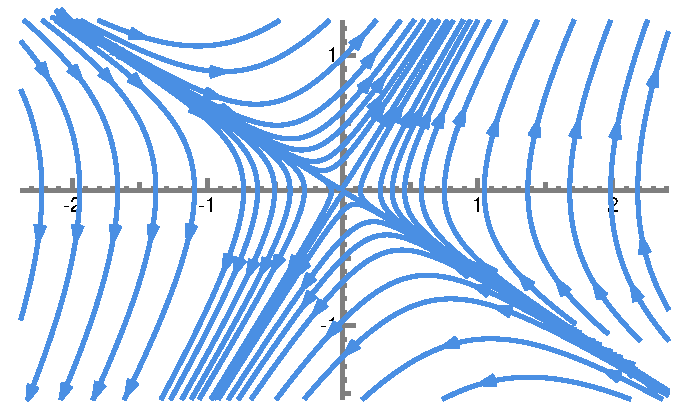
\includegraphics[width=0.75\textwidth]{sistemi_sella.pdf}
  \caption[1a]{sella (instabile)}
 \end{subfigure}
 \begin{subfigure}{5cm}
  \myurloff{sistemi_nodo}{Sistemi lineari: nodo}{21mm}%
  \centering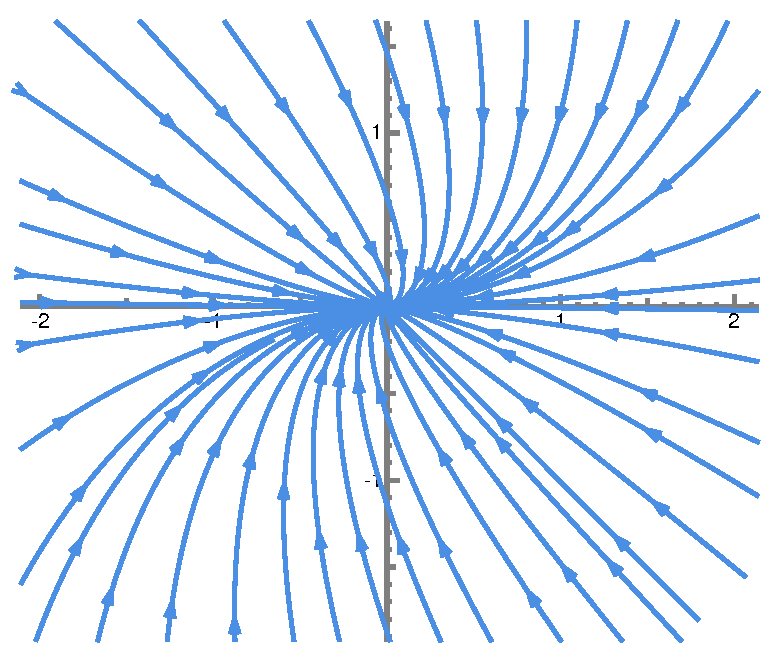
\includegraphics[width=0.75\textwidth]{sistemi_nodo.pdf}
  \caption{nodo stabile}
 \end{subfigure}
 \begin{subfigure}{5cm}
 \myurl{sistemi_nodo_improprio}{Sistemi lineari: nodo improprio}%
 \centering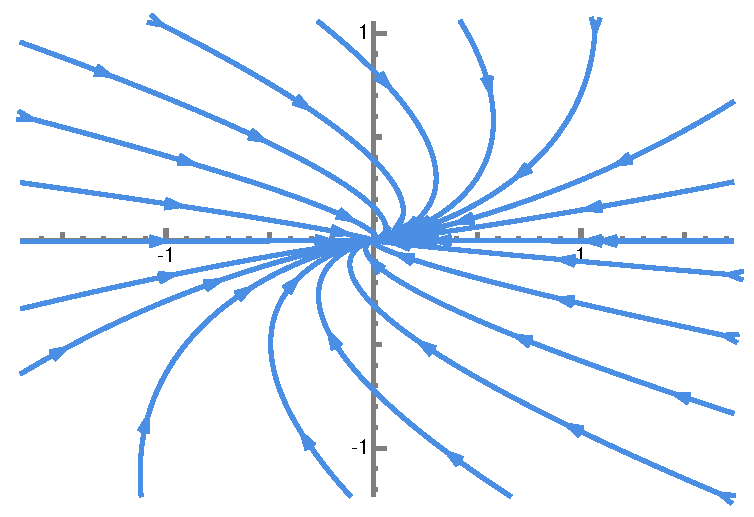
\includegraphics[width=0.75\textwidth]{sistemi_nodo_improprio.pdf}
  \caption{nodo improprio stabile}
 \end{subfigure}
 \begin{subfigure}{5cm}
  \myurloff{sistemi_stella}{Sistemi lineari: stella}{22mm}%
  \centering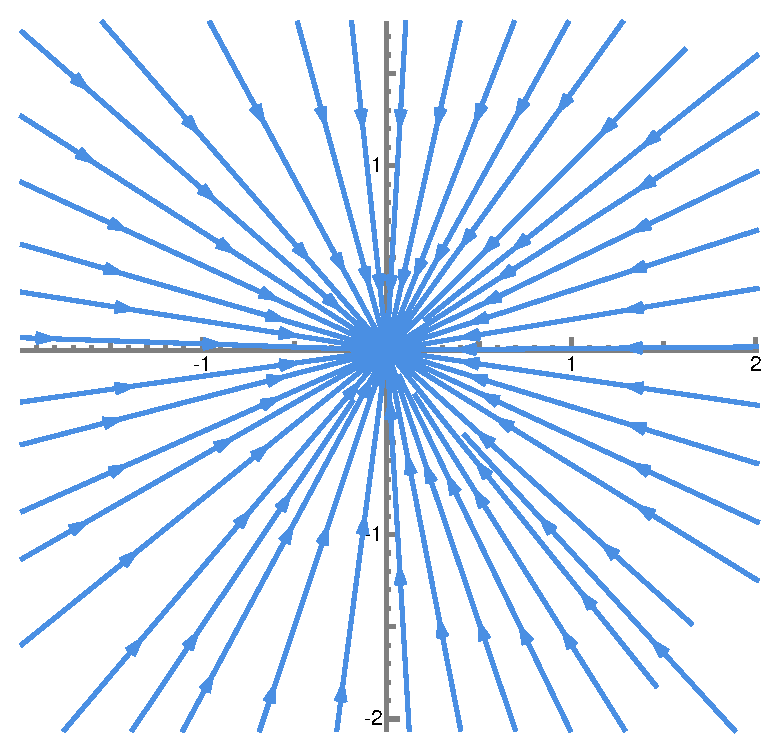
\includegraphics[width=0.75\textwidth]{sistemi_stella.pdf}
  \caption{stella stabile}
 \end{subfigure}
 \begin{subfigure}{5cm}
  \myurl{sistemi_fuoco}{Sistemi lineari: fuoco}%
  \centering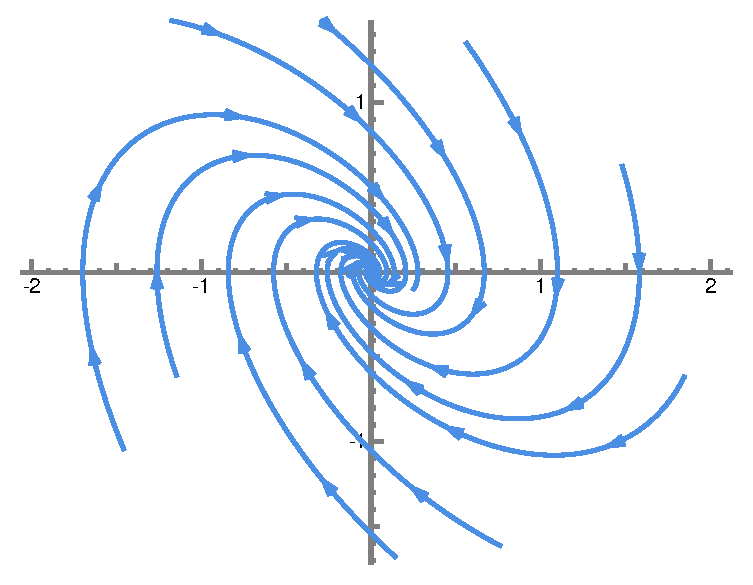
\includegraphics[width=0.75\textwidth]{sistemi_fuoco.pdf}
  \caption{fuoco stabile}
 \end{subfigure}
 \begin{subfigure}{5cm}
  \myurloff{sistemi_centro}{Sistemi lineari: centro}{21mm}%
  \centering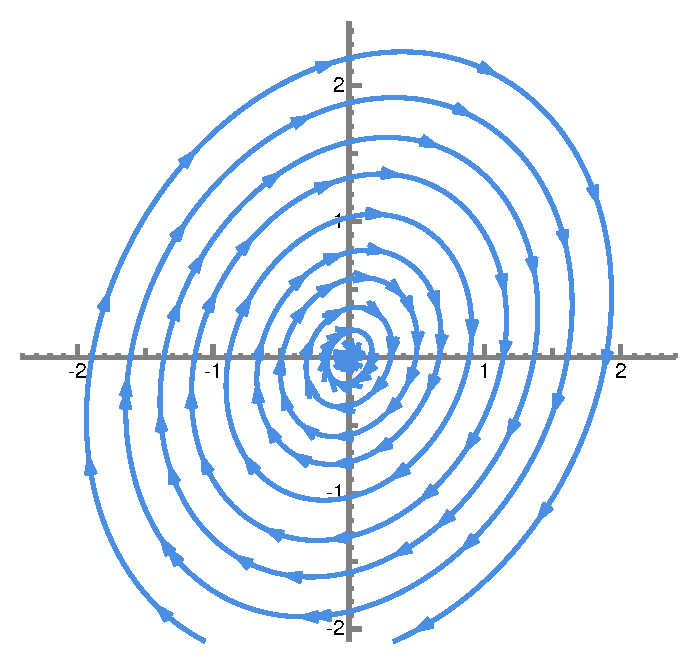
\includegraphics[width=0.75\textwidth]{sistemi_centro.pdf}
  \caption{centro (stabile)}
 \end{subfigure}
\end{figure}

Se i segni di $\lambda$ e $\mu$ sono opposti,
si ottiene una configurazione chiamata
\myemph{sella} (si veda figura).
Lungo l'autovettore con autovalore negativo
ci sarà convergenza verso l'origine, ma questa
convergenza è instabile in quanto ogni altra
curva tenderà invece a essere deviata
e a tendere asintoticamente verso la direzione
dell'autovettore con autovalore positivo.

Se $\lambda$ e $\mu$ sono entrambi negativi si
ha un \myemph{nodo stabile} in cui tutte le
curve convergono verso l'origine (soluzione
attrattiva). Se invece $\lambda$ e $\mu$
sono entrambi positivi le curve
saranno percorse in senso inverso e saranno
uscenti dall'origine: si avrà allora
un \myemph{nodo instabile}.

Se gli autovalori sono coincidenti $\lambda=\mu$
e se la matrice è diagonalizzabile allora
la matrice è diagonale, tutti i vettori sono
autovettori quindi in ogni direzione c'è
una traiettoria rettilinea.
La configurazione si
chiama \myemph{stella} (stabile o instabile a seconda
del segno negativo o positivo).

Se gli autovalori sono coincidenti $\lambda = \mu$ e la matrice
non è diagonalizzabile consideriamo l'autovettore (unico)
$\vec u$ con $A \vec u = \lambda \vec u$
e prendiamo un qualunque vettore $\vec w$
indipendente da $\vec u$. Allora si avrà
\[
  A \vec w = \alpha \vec u + \beta \vec w.
\]
Certamente $\alpha \neq 0$ altrimenti $\vec w$
sarebbe un autovettore e la matrice sarebbe diagonalizzabile.
Consideriamo allora $\vec v = \vec w / \alpha$
cosicché si ha $A \vec v = \vec u + \frac{\beta}{\alpha} \vec w$.
Nella base $\vec u, \vec v$ la matrice $A$ diventa
triangolare, e sulla diagonale troviamo i valori $\lambda$
e $\frac{\beta}{\alpha}$.
Ma allora $\frac{\beta}{\alpha} = \lambda$ in quanto sulla diagonale
abbiamo solo gli autovalori. Dunque se $X,Y$ sono le coordinate nel
sistema $\vec u, \vec v$, il sistema di equazioni diventa:
\[
\begin{cases}
X' = \lambda X + Y \\
Y' = \lambda Y.
\end{cases}
\]
Dalla seconda equazione si ottiene quindi $Y = a e^{\lambda t}$
con $a\in \RR$ costante arbitraria
e sostituendo nella prima si ottiene l'equazione
\[
  X' - \lambda X = a e^{\lambda t}
\]
che può essere risolta trovando una seconda costante arbitraria $b\in \RR$ e
\[
  X = (at+b) e^{\lambda t}.
\]
Se $a=0$ una traiettoria con $Y=0$ cioè nella direzione dell'unico autovettore.
Se $\lambda <0$ tale traiettoria sarà convergente a $0$ altrimenti sarà divergente.
Se $a\neq 0$ possiamo eliminare $t$ ponendo:
\[
  t = \frac 1 \lambda \ln \frac{Y}{a}
\]
e quindi
\[
  X = \enclose{\frac{a}{\lambda} \ln \frac{Y}{a}+ b} \frac{Y}{a}
  =  \frac{Y}{\lambda}\ln \frac{Y}{a}+ \frac{b}{a}Y.
\]
Studiando il grafico di questa funzione si ottengono qualitativamente
le curve disegnate in figura: la configurazione si chiama \myemph{nodo improprio}.
Come per i nodi le traiettorie convergono all'origine se $\lambda < 0$ e
divergono se $\lambda >0$.

Proviamo a trattare il caso, più interessante,
degli autovalori complessi. Se la matrice è a coefficienti
reali gli autovalori, quando
non reali, saranno certamente complessi coniugati:
\[
  \lambda = \alpha - i \beta,
  \qquad
  \mu = \alpha + i \beta
\]
con $\alpha,\beta\in \RR$, $\beta\neq 0$.

Sia $\vec v + i \vec w$ un autovettore complesso relativo
all'autovalore $\alpha - i \beta$.
Allora si ha
\[
 A\vec v + i A \vec w
 = A(\vec v + i \vec w)
 = (\alpha - i \beta)(\vec v + i \vec w)
 = \alpha \vec v + \beta \vec w +i(-\beta \vec v + \alpha \vec w).
\]
Uguagliando parte reale e parte immaginaria si trova
\[
  A \vec v = \alpha \vec v + \beta \vec w,
  \qquad
  A \vec w = -\beta \vec v + \alpha \vec w.
\]
A questo punto non è difficile verificare che $\vec v - i \vec w$
è un autovettore relativo all'autovalore coniugato $\alpha + i\beta$.
Visto che $\vec v\pm i\vec w$ sono due autovettori con autovalori
distinti sicuramente sono vettori indipendenti.
Dunque anche $\vec v$ e $\vec w$
(che si ottengono come multipli di somma e differenza)
sono vettori, stavolta reali
indipendenti.
Se $X,Y$ sono le coordinate nella base $\vec v$, $\vec w$, l'equazione
differenziale diventa:
\[
\begin{cases}
 X' = \alpha X - \beta Y \\
 Y' = \beta X + \alpha Y.
\end{cases}
\]
Si ha allora%
\footnote{Si potrebbe osservare che la matrice
$\begin{pmatrix}\alpha&-\beta\\ \beta & \alpha\end{pmatrix}$
è la matrice che rappresenta la moltiplicazione
complessa per il numero $\alpha + i\beta$. Dunque chiamando $Z=X+iY$
il sistema si potrebbe scrivere nella forma $Z'=(\alpha +i\beta)Z$
e si potrebbe quindi osservare immediatamente
che la soluzione deve essere della forma $Z = c e^{(\alpha+i\beta)t}$
con $c$ costante complessa. Ponendo poi $c=\rho e^{i\theta}$
si ottiene il risultato.}
\[
 X'' = \alpha X' - \beta Y'
 = \alpha X' - \beta (\beta X + \alpha Y)
\]
da cui, usando $\beta Y = \alpha X - X'$ possiamo eliminare la variabile $Y$
e ottenere una equazione del secondo ordine in $X$:
\[
 X'' = \alpha X' - \beta^2 X - \alpha (\alpha X - X')
  = 2 \alpha X' - (\alpha^2+\beta^2) X
\]
ovvero
\[
 X'' - 2 \alpha X' + (\alpha^2 + \beta^2) X = 0.
\]
Risolvendo questa equazione del secondo ordine ci si accorge
che le radici del polinomio caratteristico sono proprio $\alpha \pm i \beta$
e quindi le soluzioni si scrivono nella forma
\[
X = e^{\alpha t}(a \cos \beta t + b \sin \beta t)
\]
da cui
\begin{align*}
\beta Y
&= \alpha X - X'\\
& = \alpha e^{\alpha t}(a \cos \beta t + b \sin \beta t) \\
&\quad - \alpha e^{\alpha t}(a\cos \beta t + b \sin \beta t)
  - e^{\alpha t}(-\beta a \sin \beta t + b \beta \cos \beta t) \\
 &= \beta e^{\alpha t}(a\sin \beta t - b \cos \beta t).
\end{align*}
Dunque, ponendo $\rho=\sqrt{a^2+b^2}$ e scegliendo $\theta$
tale che $\cos \theta = \frac a \rho$ e $\sin \theta = - \frac b \rho$,
si ha
\[
  \begin{cases}
   X = \rho e^{\alpha t} \cos(\beta t + \theta),\\
   Y = \rho e^{\alpha t} \sin(\beta t + \theta).
  \end{cases}
\]
Se $\alpha \neq 0$ le traiettorie corrispondenti formano delle spirali
ellittiche che si avvitano nella direzione che porta il vettore $\vec v$ verso
il vettore $\vec w$. Se $\alpha < 0$ le spirali convergono verso l'origine del
sistema: avremo un \myemph{fuoco stabile}. Se $\alpha >0$ le orbite
divergono chiameremo la configurazione un \myemph{fuoco instabile}.
Se $\alpha = 0$ le traiettorie sono delle ellissi concentriche,
le soluzioni sono quindi periodiche e la configurazione
si chiama \myemph{centro}.

Se almeno uno dei due autovalori è nullo il comportamento del sistema è degenere,
si hanno delle soluzioni banali che non andremo a investigare.

\subsection{matrice esponenziale}

Per risolvere, in astratto, il sistema $n\times n$ del primo ordine, 
lineare omogeneo a coefficienti costanti
\[
  \vec u' = A \vec u
\]
introduciamo le seguenti nozioni.

Sia $A$ una matrice quadrata $n\times n$. Definiamo la norma (norma
operatoriale) di $A$ come segue:
\[
  \Abs{ A } = \sup_{\abs{\vec v} \le 1} \abs{A\vec v}
\]
dove $\abs{ \vec v} = \sqrt{v_1^2+ \dots + v_n^2}$ è l'usuale norma del
vettore $\vec v\in \RR^n$.
Osserviamo che $\vec v\mapsto A\vec v$ è una funzione
continua e che $\ENCLOSE{\vec v\colon \abs{ \vec v} \le 1}$ è un insieme
compatto, dunque il $\sup$ nella definizione è in realtà un $\max$.

Per le proprietà del $\sup$ si ha:
\[
  \abs{A\vec v} \le \Abs{ A }\, \abs{ v }
\qquad\text{e}\qquad
  \Abs{ A B } \le \Abs{ A } \, \Abs{ B }.
\]
Dunque possiamo affermare il valore assoluto di ogni elemento di una
matrice si stima con la norma della matrice: $\abs{ A_{ij}} \le
\Abs{ A }$, infatti:
\[
  \abs{ A_{ij} } = \abs{ (A \vec e_j)_i} \le \abs{ A e_j}
  \le \Abs{ A }
\]
(dove $\vec e_j$ è il $j$-esimo vettore della base canonica di $\RR^n$).

Se $A_k$ è una successione di matrici, diremo che $A_k\to A$ se ogni
elemento della matrice $A_k$ converge al corrispondente elemento della
matrice $A$: $(A_k)_{ij} \to A_{ij}$. Questo corrisponde a considerare
la matrice $n\times n$ come un vettore dello spazio $\RR^{(n^2)}$.

Se $A(t)$ è una funzione a valori matrici (ovvero una matrice i cui
elementi sono funzioni di $t$), si potrà farne la derivata
come si fa per le funzioni vettoriali: $(A'(t))_{ij} = (A_{ij}(t))'$
cioè componente per componente. Le usuali regole per le derivate
valgono anche per le matrici, in particolare non è difficile
verificare (si espliciti la definizione del prodotto di matrici) che
\[
 (A(t)B(t))' = A'(t) B(t) + A(t) B'(t)
\]
dove, puntualizziamo, è importante mantenere i prodotti nell'ordine
giusto, in quanto il prodotto di matrici può non essere commutativo.

Se $A$ è una matrice quadrata, si definisce la matrice potenza $A^k$
per ogni $k$ naturale, mediante le proprietà
\[
  A^0 = I, \qquad A^{k+1} = A^kA.
\]
(se $A$ è invertibile si possono definire anche le potenze negative
$A^{-k}=(A^{-1})^k = (A^k)^{-1}$).

Definiamo allora la matrice esponenziale di $A$:
\[
  e^A = \sum_{k=0}^\infty \frac{A^k}{k!}.
\]
Per dare significato a questa definizione dobbiamo verificare che la
serie appena scritta sia convergente. Cioè dobbiamo verificare che per
ogni coppia di indici $ij$ sia convergente la serie numerica:
\[
 \sum_{k=0}^\infty \frac{(A^k)_{ij}}{k!}.
\]
Per quanto detto prima sappiamo che
$\abs{(A^k)_{ij}} \le \Abs{A^k} \le \Abs{A}^k$.
Dunque la serie in questione è
assolutamente convergente in quanto il suo valore assoluto si stima
con la serie
\[
 \sum_{k=0}^\infty \frac{\Abs{ A}^k}{k!} = e^{\Abs{ A}}
\]
che è convergente. La definizione della matrice $e^A$ è dunque
ben posta e si ha
\[
 \Abs{ e^A} \le e^{\Abs{ A }}.
\]

\begin{theorem}[proprietà dell'esponenziale matrice]
Siano $A$ e $B$ matrici quadrate $n\times n$ e $t$ uno scalare.
Valgono le seguenti proprietà:
\begin{enumerate}
\item $e^0 = I$ (dove $0$ è la matrice nulla $n\times n$ ed $I$ è la
  matrice identità con le stesse dimensioni);
\item se $AB=BA$ allora $e^A B = B e^A$;
\item $(e^{tA})' = A e^{tA}$;
\item $e^{-A} = (e^A)^{-1}$ (in particolare la matrice esponenziale è
  sempre invertibile);
\item se $\vec u(t)$ è una funzione a valori in $\RR^n$ che soddisfa
  l'equazione differenziale $\vec u'(t) = A\vec u(t)$ allora
  $\vec u(t) = e^{tA} \vec u(0)$;
\item se $AB=BA$ allora $e^{A+B} = e^A e^B$;
\item se $A$ è invertibile allora $e^{ABA^{-1}} = Ae^BA^{-1}$;
\item se $A$ è la matrice diagonale $A = \diag(\lambda_1, \dots, \lambda_n)$,
allora $e^A$
 è pure una matrice diagonale con $e^A = \diag(e^{\lambda_1},\dots, e^{\lambda_n})$;
\item se $A$ è una matrice triangolare con la diagonale nulla (cioè
  $A_{ij}=0$ se $i\ge j$) allora $e^A = \sum_{k=0}^n \frac{A^k}{k!}$
  (basta sommare i primi $n+1$ termini);
\item se $B$ è una matrice triangolare (cioè $B_{ij}=0$ se $i > j$)
  allora $B = D + A$ con $D$ matrice diagonale e $A$ matrice
  triangolare con la diagonale nulla e quindi $e^B = e^De^A$ si può
  calcolare riconducendosi ai punti precedenti.
\end{enumerate}
\begin{proof}
1. Per quanto riguarda $e^0$ osserviamo che per definizione $0^0=I$
mentre $0^k=0$ se $k>0$. Dunque direttamente dalla definizione si
ottiene $e^0=I$.

2. Se $AB=BA$ osserviamo che si ha anche $A^k B=B A^k$ (la matrice $B$
commuta con ogni fattore del prodotto $A^k$). Dunque:
\[
 \sum_{k=0}^N \frac{A^k}{k!} B = B \sum_{k=0}^N \frac{A^k}{k!}
\]
e passando al limite $N\to \infty$ si ottiene $e^A B = B e^A$.

3. Per calcolare la derivata di $e^{tA}$ vogliamo dimostrare che la serie
che definisce $e^{tA}$ converge totalmente quando $t$ varia in un
qualunque intervallo limitato. Poniamo allora $t\in [-M,M]$. Si ha:
\[
  \sup_{t\in[-M,M]}\frac{\Abs{ (tA)^k}}{k!}
  = \sup_{t\in[-M,M]}\frac{\abs{ t}^k \Abs{ A^k}}{k!}
  \le \frac{M^k\Abs{ A}^k}{k!}
\]
la cui serie è convergente qualunque sia $M\in \RR$. Dunque la serie
che definisce $e^{tA}$ è una serie di funzioni continue e derivabili
che converge totalmente su ogni intervallo limitato. Possiamo quindi
derivare la serie termine a termine:
\[
(e^{tA})' = \sum_{k=0}^\infty \frac{((tA)^k)'}{k!}
 = \sum_{k=1}^\infty \frac{kt^{k-1} A^k}{k!}
 = A \sum_{k=1}^\infty \frac{t^{k-1}A^{k-1}}{(k-1)!}
 = A e^{tA}.
\]

4. Dimostriamo ora che $U(t) = e^{tA}e^{-tA}=I$ per ogni $t$. Si ha:
\[
 U'(t) = A e^{tA}e^{-tA} + e^{tA}(-A)e^{-tA}
       = A e^{tA}e^{-tA} - A e^{tA}e^{-tA} = 0
\]
($Ae^{tA} = e^{tA}A$ in quanto $A$ e $tA$ commutano).
Dunque $U'(t)=0$ cioè $U(t)$ è costante ovvero $U(t)=U(0)$. Ma $U(0)=I$
in quanto $e^0=I$ e quindi $U(t)=I$ per ogni $t$.

5. Prendiamo l'equazione $\vec u' = A\vec u$, moltiplicando a sinistra per
$e^{-tA}$ l'equazione diventa
$e^{-tA} \vec u' - e^{-tA} A \vec u=0$ cioè $(e^{-tA} \vec u)' = 0$. Questo significa
che la funzione $e^{-tA}\vec u = c$ costante e moltiplicando a sinistra per
$e^{tA}$ si ottiene dunque $\vec u = e^{tA}c$ come volevasi dimostrare.

6. Per dimostrare la proprietà $e^{A+B}=e^A e^B$ consideriamo la quantità
$U(t) = e^{-t(A+B)} e^{tA} e^{tB}$. Se dimostriamo che $U$ è costante,
visto che $\vec u(0)=I$ si avrà anche $U(1)=I$ che è equivalente a quanto
vogliamo dimostrare. Dunque verifichiamo che la derivata è nulla,
sfruttando l'ipotesi $AB=BA$ che ci permette di far commutare i prodotti:
\begin{align*}
U'(t) & = -(A+B)e^{-t(A+B)} e^{tA} e^{tB} + e^{-t(A+B)}Ae^{tA}e^{tB} +
e^{-t(A+B)}e^{tA} B e^{tB} \\
& = [-(A+B) + A + B] U(t) = 0.
\end{align*}

7. Se $A$ è invertibile allora $(ABA^{-1})^k = ABA^{-1}ABA\dots ABA^{-1}
= AB^k A^{-1}$. Dunque nelle somme parziali della serie che definisce l'esponenziale
$e^{ABA^{-1}}$ si può raccogliere $A$ a sinistra e $A^{-1}$ a destra e
al centro rimane la serie che definisce $e^B$.

8. Se la matrice $A$ è diagonale con $A_{ii}=\lambda_i$ allora $A^k$
risulta essere una matrice diagonale con $(A^k)_{ii} =
\lambda_i^k$. Dunque nella definizione di esponenziale $e^A$ i termini
della serie sono tutte matrici diagonali, e sulla diagonale compare la
serie che definisce l'esponenziale $e^{\lambda_i}$.

9. Se $A$ è una matrice triangolare con $A_{ij}=0$ quando $i\ge j$, si
osserva che $A^2$ avrà degli zeri anche sopra la diagonale:
$(A^2)_{ij}=0$ quando $i+1\ge j$ (si applichi la definizione di
prodotto, riga per colonna). Nelle moltiplicazioni successive $A^3,
A^4,\dots$ si aggiungerà sempre una diagonale di zeri finché la matrice non
si annulla completamente $A^n=0$. Dunque la serie che definisce $e^A$
contiene solo un numero finito di termini (i primi $n+1$) e può essere
calcolata esplicitamente.

10. L'ultima proprietà è una osservazione che non richiede dimostrazione.
\end{proof}
\end{theorem}

\section{studio qualitativo delle soluzioni}

Non sempre è possibile determinare esplicitamente le soluzioni
di una equazione differenziale.
Ci proponiamo quindi di trovare dei metodi per
determinare alcune proprietà salienti delle soluzioni, senza
doverle determinare esplicitamente.
Considereremo unicamente equazioni del primo ordine in forma normale:
\begin{equation}\label{eqdiff}
	u'(x)= f(x,u(x))
\end{equation}
con $f\colon \Omega \subset \RR^2\to \RR$.

Ricordiamo che se $f$ soddisfa la condizione di Cauchy-Lipschitz
(definizione~\ref{def:cauchy_lipschitz}), in particolare
se $f$ è di classe $C^1$ allora i grafici delle soluzioni
massimali dell'equazione differenziale~\eqref{eqdiff}
\emph{fibrano} la regione $\Omega$ nel senso che per ogni punto di
$\Omega$ passa una unica soluzione massimale (teorema~\ref{th:cauchy_lipschitz}
di Cauchy-Lipschitz e proposizione~\ref{prop:separazione_soluzioni}).
Inoltre la proposizione~\ref{prop:edo_massimale} ci dice
che le soluzioni massimali escono da qualunque compatto contenuto in
$\Omega$ ovvero raggiungono sempre la frontiera di $\Omega$.

\begin{example}\label{ex:edo_463}
Dimostrare che il seguente problema di Cauchy
\[
	\left\{ \begin{array}{l}
		u'(x) = (u^2(x)-1)\cdot x\cdot \sin x \\
		u(0) = 0
	\end{array}\right.
\]
ammette una unica soluzione massimale $u(x)$
definita su tutto $\RR$ (dunque la soluzione è globale).
\end{example}
\begin{figure}
  \myurl{edo_463}{Studio qualitativo esempio~\ref{ex:edo_463}}
  \centering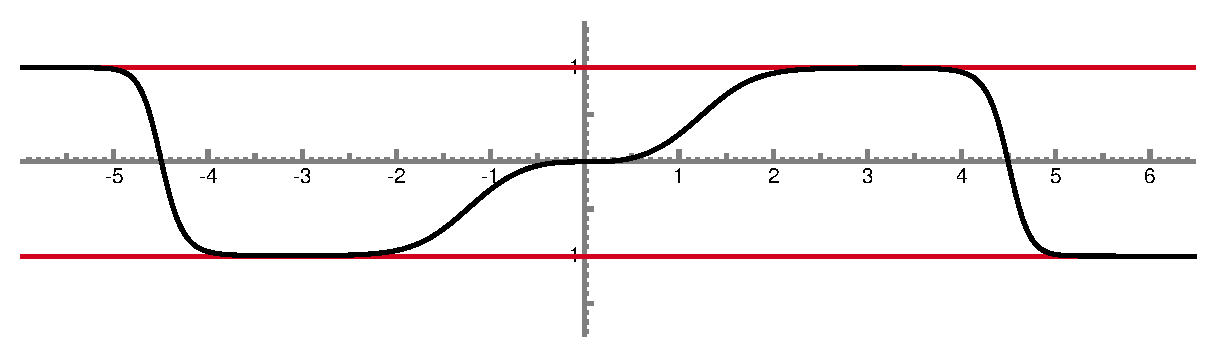
\includegraphics[width=\textwidth]{edo_463}
  \label{fig:edo_463}
  \caption{Studio qualitativo dell'esempio~\ref{ex:edo_463}}
\end{figure}
%
\begin{proof}[Svolgimento.]
In questo caso si ha $f(x,y)=(y^2-1)x\sin x$, che \`e una funzione
di classe $\CC^1$ su tutto $\Omega=\RR^2$.
Vale dunque il teorema di esistenza ed
unicità delle soluzioni.
Notiamo inoltre (per verifica diretta)
che $u_0(x)=-1$ e $u_1(x)=1$ sono
soluzioni costanti dell'equazione differenziale (\ref{eqdiff})
in quanto $f(x,-1)=f(x,1)=0$ per ogni $x\in \RR$
(se $x$ rappresenta il tempo le soluzioni costanti si chiamano
anche \emph{stazionarie}).
Il grafico della soluzione $u(x)$ dunque
non può toccare i grafici delle due funzioni $u_0=-1$ e $u_1=1$ e visto
che $u(0)=0$ e che $u$ è una funzione continua significa
che per ogni $x$ si ha $-1 < u(x) < 1$.
Consideriamo ora il compatto
$K_M=[-M,M] \times [-1,1]$.
Sappiamo che la soluzione
massimale $u(x)$ del problema di Cauchy preso in considerazione deve
uscire da ogni compatto $K_M$.
Visto però che $u(x)\in (-1,1)$ significa che necessariamente
il grafico della soluzione massimale $u(x)$
raggiunge i due segmenti verticali
$x=-M$ e $x=M$ e dunque l'intervallo massimale di esistenza
contiene l'intervallo $[-M,M]$.
Siccome questo è vero per ogni $M$, l'intervallo massimale
di esistenza della soluzione è $I=\RR$ e dunque la soluzione
è globale.
\end{proof}

\subsection{monotonia e punti critici delle soluzioni}

Dopo aver determinato le zone di $\Omega$ su cui vale il teorema di
esistenza e unicit\`a, \`e utile studiare il segno di $f$. Infatti
le soluzioni $u(x)$ dell'equazione differenziale (\ref{eqdiff})
saranno strettamente crescenti dove $f>0$, strettamente decrescenti
dove $f<0$ e avranno un punto critico dove $f=0$.

Un primo caso notevole è il caso in cui $f$ si annulla su una
retta orizzontale $y=c$.
In questo caso la funzione costante $u(x)=c$ è una
soluzione dell'equazione differenziale (\ref{eqdiff}).
Inoltre
(nell'ipotesi $f\in\CC^1$) tale costante non può essere
attraversata dalle altre soluzioni dell'equazione differenziale.

\`E importante capire se le soluzioni dell'equazione differenziale
attraversano o no la curva $\{f=0\}$. Infatti questo ci permette di
determinare il segno della derivata $u'(x)$ e quindi di ottenere
importanti informazioni sull'andamento della soluzione $u(x)$
(monotonia, massimi e minimi relativi...).

Più in generale è interessante capire quando una soluzione di una
equazione differenziale può attraversare una determinata curva.

\begin{theorem}\label{nonpassa}
Sia $u(x)$ una soluzione dell'equazione differenziale $(\ref{eqdiff})$
definita su un intervallo $I$ e sia $u_0(x)$ una funzione qualunque
definita su $I$, di classe $\CC^1$ e tale che il suo grafico sia
interamente contenuto nel dominio $\Omega$ di definizione di $f$.
Supponiamo che in un punto fissato $x_0$ interno ad $I$ si abbia
$u(x_0)<u_0(x_0)$ e supponiamo inoltre che per ogni $x>x_0$ si abbia
$u_0'(x)>f(x,u_0(x))$. Allora per ogni $x>x_0$ si ha $u(x)<u_0(x)$.

Analogamente se $u(x_0)>u_0(x_0)$ e se per ogni $x$ si ha
$u_0'(x)<f(x,u_0(x)$ risulterà $u(x)>u_0(x)$ per ogni $x>x_0$.

Risultati analoghi si hanno per $x<x_0$.
\end{theorem}

\begin{proof}
Supponiamo per assurdo che l'insieme $J=\{x\in I: x\ge x_0\
\mathrm{e}\ u(x)=u_0(x)\}$ non sia vuoto.
Tale insieme è chiuso ed
inferiormente limitato, quindi se non è vuoto, ammette minimo.
Sia $\bar x$ il minimo di $J$.
Sicuramente $\bar x>x_0$ in quanto $u(\bar
x)=u_0(\bar x)$.
Inoltre per ogni $x\in \left[x_0,\bar x\right[$ si ha
$u(x)-u_0(x)<0$ e quindi $u'(\bar x) \ge u_0'(\bar x)$ (in quanto
il rapporto incrementale sinistro di $y-y_0$ è sempre positivo).

Questo è assurdo in quanto per ipotesi si ha invece $u'(\bar x) =
f(\bar x, u(\bar x)) = f(\bar x ,u_0(\bar x)) < u_0'(\bar x)$.
\end{proof}

Se ad esempio $u_0(x)$ è una funzione
il cui grafico è contenuto in $\{f=0\}$
(cioé $f(x,u_0(x))=0$) allora una soluzione $u(x)$ dell'equazione
differenziale può attraversare la curva $u_0(x)$ dall'alto verso il
basso nei punti in cui $u'_0(x)>0$ e dal basso verso l'alto nei punti
in cui $u'_0(x)<0$.

\begin{example}
Mostrare che il seguente problema di Cauchy
\[
\left\{\begin{array}{l}
  u'=1-x u^3\\
  u(0)=0
	\end{array}\right.
\]
ammette una soluzione $u(x)$ definita su tutto $\RR$.
\end{example}
%
\begin{proof}[Svolgimento.]
Posto $f(x,y)=xy^3$ abbiamo che $f$ si annulla sul grafico della
funzione $u_0(x)=1/\sqrt[3] x$. Per $x>0$ la soluzione è crescente
quando si trova al di sotto della funzione $u_0$ ed è decrescente
quando si trova al di sopra. Inoltre essendo $u_0'<0$ le soluzioni possono
attraversare la funzione $u_0(x)$ solo passando da sotto a
sopra.

Sia $u(x)$ la soluzione del problema di Cachy in questione, definita su
un intervallo massimale $I$. Il dato
iniziale è $(0,0)\in \{f>0\}$. Dunque la soluzione risulta essere
strettamente crescente in un intorno di $0$.

Vogliamo dimostrare innanzitutto che necessariamente la soluzione
incontra entrambi i rami del grafico di $u_0(x)$. Sia infatti
$\epsilon>0$ sufficientemente piccolo da appartenere all'intervallo
$I$ di
esistenza della soluzione e sia $\delta=u(\epsilon)$.
Consideriamo il compatto $K=\{(x,y):
\epsilon/2 \le x \le 1/\delta^2,\ 0\le y\le 1/sqrt{x}\}$. Il punto
$(\epsilon,u(\epsilon))$ è interno al compatto $K$ ma la soluzione deve
uscire dal compatto
per un qualche $x>\epsilon$.
La soluzione però non può toccare la
retta $y=0$ in quanto all'interno del compatto rimane sempre positiva
e crescente.
Non può neanche toccare il segmento verticale
$x=1/\delta^2$, $y\in[0,\delta]$ in quanto $u(\epsilon)=\delta$ e per
$x>0$ la soluzione è strettamente crescente.
Dunque necessariamente
la soluzione deve incontrare il grafico della funzione
$u_0(x)=1/\sqrt{x}$ in un punto $\bar x>0$.

Nel punto $x=\bar x$ la soluzione $u(x)$ attraversa la curva
$u_0(x)$. Infatti in tale punto $u'(\bar x)=0$ mentre $u_0'(\bar
x)<0$.
Dunque in un intorno destro di $\bar x$ la soluzione si trova
al di sopra della curva $u_0(x)$ e quindi risulta essere decrescente
(in $\bar x$ la soluzione presenta un massimo relativo).

Il Teorema~\ref{nonpassa} garantisce inoltre che la soluzione non
può più riattraversare il grafico della funzione $u_0$ in quanto
$u'_0<0$. Dunque la soluzione è decrescente e limitata.
Dunque (usando come al solito la proposizione~\ref{prop:edo_massimale})
possiamo dedurre che la soluzione massimale è definita per ogni $x>0$.

Un ragionamento analogo si fa per $x<0$ ottenendo l'esistenza globale
della soluzione.
\end{proof}

\begin{example}
Dimostriamo che il problema di Cauchy
\[
\begin{cases}
	u' = -x(u^3 - \sin x) \\
	u(0) = 0
\end{cases}
\]
ammette una soluzione $u(x)$ definita su tutto $\RR$.
\end{example}
%
\begin{proof}
Sia $u(x)$ la soluzione massimale del problema di Cauchy
definita su un intervallo massimale $I$.

Mostriamo innanzitutto che $\vert u(x) \vert < 2$ per ogni $x\in
I$.
Infatti per $x>0$ sulla curva $u_1(x)=2$ si ha $f(x,2) = -x
(8-\sin x) < -x < 0 = u_1'(x)$.
Dunque per il Teorema~\ref{nonpassa} la
soluzione per $x>0$ non può mai attraversare la retta
$y=2$.
Discorso analogo si fa per la retta $y=-2$ e anche per $x<0$
mostrando che il grafico della  soluzione non può mai toccare le
rette $y=2$ e $y=-2$ né per $x>0$ né per $x<0$
e che quindi $u(x)$ risulta limitata (in realtà si
può essere più precisi e mostrare che $\vert u(x)\vert \le 1$).

A questo punto si applica, come al solito, il Teorema~\ref{prop:edo_massimale} ai
compatti $K_M=[-M,M]\times[-2,2]$ mostrando che la soluzione deve
avere esistenza globale.
\end{proof}

\subsection{teoremi di confronto}

\begin{theorem}
Sia $I\subset \RR$ un intervallo su cui sono definite due funzioni derivabili
$f(x)$ e $g(x)$.
Siano $x_0<x_1$ due punti di $I$. Se $f(x_1)<g(x_1)$ e $f(x_2)>g(x_2)$
allora esiste un punto $\bar x \in (x_1,x_2)$ tale che $f(\bar
x)=g(\bar x)$ e $f'(\bar x)\ge g'(\bar x)$.
\end{theorem}

\begin{theorem}
Consideriamo due funzioni $u(x)$ e $v(x)$ soluzioni dei rispettivi
problemi di Cauchy
\[
\begin{cases}
  u'(x)  = f(x,u(x))\\
  u(x_0) = u_0
\end{cases}
\qquad
\begin{cases}
  v'(x) = g(x,v(x))\\
  v(x_0) = v_0
\end{cases}
\]
su un intervallo $I$ che contiene il punto $x_0$.
Sia $\Omega\subset \RR^2$ un sottoinsieme degli insiemi di definizione
di $f$ e $g$ tale che i grafici delle soluzioni $u(x)$ e $v(x)$ siano
contenuti in $\Omega$ al variare di $x\in I$.
Supponiamo che per ogni $(x,y)\in\Omega$ si abbia $f(x,y)<g(x,y)$.
Allora per ogni $x\in I$, $x> x_0$ si ha $u(x)< v(x)$ mentre per ogni
$x\in I$, $x<x_0$ si ha $u(x)>v(x)$.
\end{theorem}

\begin{theorem}
Sia $f\colon (x_0,+\infty)\to \RR$ una funzione di classe
$C^1$ tale
che il limite
\[
  \lim_{x\to +\infty} f'(x) = \ell
\]
esiste, finito o infinito. Se $\ell\neq 0$ allora $f$ non può avere
un asintoto orizzontale per $x\to +\infty$.
\end{theorem}


\backmatter

%\chapter{richiami di algebra lineare}

\begin{definition}[autovalori e autovettori]
Sia $V$ uno spazio vettoriale sul campo $\KK$ (con $\KK = \RR$ o $\KK=\CC$)
e $A\colon V\to V$ un operatore lineare.
Diremo che $\lambda\in \KK$ è un \myemph{autovalore} di $A$
e esiste $v\in V$, $v\neq 0$ tale che
\[
  Av = \lambda v.
\]
In tal caso $v$ si dice essere un \myemph{autovettore} di $A$ relativo
all'autovalore $\lambda$.

Denotiamo con $A-\lambda$ l'operatore lineare $A-\lambda I$
dove $I\colon V\to V$ è l'identità.
Lo spazio vettoriale
\[
  \ker (A-\lambda I)
\]
si chiama \myemph{autospazio} relativo all'autovalore $\lambda$.
L'autospazio è composto dal vettore $0$ e da tutti gli autovalori
relativi all'autovalore $\lambda$.

Diremo che $v$ è un autovettore generalizzato di grado $m$ ($m\ge 1$ intero)
relativo all'autovalore $\lambda$
se
\[
 (D-\lambda)^m v = 0
 \qquad \text{ma} \qquad
  (D-\lambda)^{m-1} v \neq 0.
\]

Gli autovettori generalizzati di grado $1$ sono esattamente gli
autovettori.
\end{definition}

\begin{proposition}[proprietà degli autovettori]
Sia $A\colon V \to V$ un operatore lineare.
Denotiamo con
\[
  W_\lambda^m = \ker (A-\lambda)^m \setminus \ker (A-\lambda)^{m-1}
\]
l'insieme (non è uno spazio vettoriale!) di tutti gli autovettori
generalizzati di $A$ di grado $m$ relativi all'autovalore $\lambda$.
Allora se $\lambda \neq \mu$ si ha
\begin{enumerate}
\item autovettori relativi ad autovalori distinti sono distinti:
\[
W_\lambda^1 \cap W_\mu^1 = \emptyset;
\]
\item gli operatori $A-\lambda$ e $A-\mu$ commutano:
\[
  (A-\lambda)(A-\mu)v = (A-\mu)(A-\lambda);
\]
\item
l'operatore $A-\mu$ lascia invariati gli insiemi $W_\lambda^m$:
\[
  v\in W_\lambda^n
  \implies
  (D-\mu)v \in W_\lambda^n.
\]
\end{enumerate}
\end{proposition}
%
\begin{proof}
\begin{enumerate}
\item
Se esistesse $v\in W_\lambda^1 \cap W_\lambda^1$ si avrebbe
\[
(\lambda - \mu) v = \lambda v - \mu v = Av - Av = 0.
\]
Ma questo è impossibile se $v\neq 0$ e $\mu\neq \lambda$.

\item
Si ha
\[
  (A-\lambda)(A-\mu)
  = A(A-\mu I) - \lambda (A-\mu I)
  = A^2 - \mu A -\lambda A + \lambda \mu I
  = A^2 - (\mu+\lambda) A + \lambda\mu I.
\]
Visto che il lato destro dell'uguaglianza è invariante se
scambiamo $\lambda$ e $\mu$ anche il lato sinistro deve esserlo.

\item
Se $(A-\lambda)^m v = 0$ si ha
\[
(A-\lambda)^m (A-\mu) v = (A-\mu)(A-\lambda^m) v = 0.
\]
Vogliamo mostrare che se $(A-\lambda)^{m-1} v \neq 0$
allora anche $(A-\lambda)^{m-1} v \neq 0$.

\end{enumerate}
\end{proof}

\appendix
\chapter{Listati}

Il seguente codice è scritto in \myemph{python}, un linguaggio di programmazione
molto semplice e pulito che permette, tra l'altro, di utilizzare diverse librerie
utili per il calcolo numerico e scientifico.

\lstset{% general command to set parameter(s)
  basicstyle=\tiny, % print whole listing small
  keywordstyle=\color{black}\bfseries\underbar,
  % underlined bold black keywords
  identifierstyle=, % nothing happens
  commentstyle=\color{white}, % white comments
  stringstyle=\ttfamily, % typewriter type for strings
  showstringspaces=false} % no special string spaces

\section{series.py}

Vedi esempio~\ref{ex:52573}.
\myqrcode{https://github.com/paolini/AnalisiUno/blob/master/code/series.py}{github}{series.py}
\label{code:series}
\lstinputlisting{code/series.py}


\section{bisection.py}

Vedi esempio~\ref{ex:75445}.
\myqrcode{https://github.com/paolini/AnalisiUno/blob/master/code/bisection.py}{github}{bisection.py}
\label{code:bisection}
\lstinputlisting{code/bisection.py}

\newpage

\section{compute\_e.py}

Vedi tabella~\ref{fig:cifre_e}.
\myqrcode{https://github.com/paolini/AnalisiUno/blob/master/code/compute_e.py}{github}{compute_e.py}
\label{code:compute_e}
\lstinputlisting{code/compute_e.py}

\section{Mandelbrot.py}

Vedi figura~\ref{fig:mandelbrot}.
\myqrcode{https://github.com/paolini/AnalisiUno/blob/master/code/Mandelbrot.py}{github}{Mandelbrot.py}
\label{code:Mandelbrot}
\lstinputlisting{code/Mandelbrot.py}

\newpage

\section{compute\_pi.py}

Vedi osservazione~\ref{rem:cifre_pi}.
\myqrcode{https://github.com/paolini/AnalisiUno/blob/master/code/compute_pi.py}{github}{compute_pi.py}
\label{code:compute_pi}
\lstinputlisting{code/compute_pi.py}

\section{Koch.py}

Vedi figura~\ref{fig:koch}.
\myqrcode{https://github.com/paolini/AnalisiUno/blob/master/code/Koch.py}{github}{Koch.py}
\label{code:Koch}
\lstinputlisting{code/Koch.py}

\newpage
\section{Fourier.py}

Vedi figura~\ref{fig:fourier}
\myqrcode{https://github.com/paolini/AnalisiUno/blob/master/code/Fourier.py}{github}{Fourier.py}
\label{code:Fourier}
\lstinputlisting{code/Fourier.py}


\nocite{Giusti}
\nocite{Courant}
\nocite{Marcellini}
\nocite{Rudin}
\nocite{PaganiSalsa}
\nocite{appunti_logica}

\bibliographystyle{plain}
\bibliography{biblio}

\printindex

\end{document}
